\documentclass[justified,a4paper,symmetric,nobib]{tufte-book}

% Packages setup
\usepackage[brazil,safe=bib]{babel}
\usepackage{hyphenat}
\usepackage[backend=biber, style = verbose, citetracker=true]{biblatex}
\renewcommand{\cite}[2][0pt]{\sidenote[][#1]{\fullcite{#2}}} % citations as sidenotes
%\newcommand{\apud}[3][0pt]{\sidenote[][#1]{\fullcite{#2} \textsc{apud} \fullcite{#3}}}

%\usepackage{bookmark} % Dá problema com o tamanho da fonte dos captions
%\hypersetup{hidelinks=true,unicode}

\usepackage[T1]{fontenc} 
\usepackage[utf8]{inputenc}						% Pacotes pra escrever
\usepackage[brazil]{babel}						% em português
%\usepackage[fixlanguage]{babelbib}
%\usepackage{biblatex}
\usepackage[np]{numprint}
\usepackage{mathcomp}
\usepackage{amsmath}
\usepackage{amssymb}
\usepackage{lipsum}
\usepackage{tikz}
\usepackage{gnuplot-lua-tikz}
\usepackage{mathtools}
%\usepackage[small, sc]{caption}
\let\tuftemarginnote\marginnote
\let\marginnote\relax
\usepackage{marginnote}
\usepackage[framemethod=default]{mdframed}
\usepackage{booktabs}
\usepackage{colortbl}
\usepackage{lscape}
\usepackage{rotating}
\usepackage{url}
\usepackage{ccicons}
\usepackage[counter-within=section,load-headings]{exsheets}
\SetupExSheets{headings=runin-wp}
\SetupExSheets[points]{name=ponto/s}
\usepackage{pifont}
\usetikzlibrary{shadows}
\usetikzlibrary{arrows.meta}
\usetikzlibrary{decorations.markings}
\usetikzlibrary{decorations.pathmorphing}
\usetikzlibrary{calc,positioning,intersections,quotes}
\usetikzlibrary{patterns,bending}
\usetikzlibrary{angles}
\usetikzlibrary{babel}
\usetikzlibrary{calendar}
\usetikzlibrary{fadings}
\usepackage{tkz-euclide}
\usepackage[siunitx,RPvoltages]{circuitikz}
\usepackage{microtype}
\usepackage{booktabs}
\usepackage{graphicx}
\setkeys{Gin}{width=\linewidth,totalheight=\textheight,keepaspectratio}
\usepackage{fancyvrb}
\fvset{fontsize=\normalsize}
\usepackage{xspace}
%\usepackage{units}
\usepackage{nicefrac}
\usepackage{longtable}
\usepackage[euler]{textgreek}
\usepackage{mparhack} % Fix footnotes positioning problem
\usepackage{wasysym}
\usepackage{enumitem}

\usetikzlibrary{external}
\tikzexternalize

% Abaixo vão os comandos para usar vírgula na pontuação das questões nos
% questionários de cada experiência (as questões em si são formatadas
% pelo pacote exsheets
\usepackage[locale=DE]{siunitx}
\usepackage{tasks}
\ExplSyntaxOn
\cs_set_protected:Npn \exsheets_num:n #1
 {
  \num{\fp_eval:n{#1}}
 }
\ExplSyntaxOff

\titleformat{\paragraph}%
  [hang]% shape
  {\normalfont\scshape}% format applied to label+text
  {\theparagraph}% label
  {1em}% horizontal separation between label and title body
  {}% before the title body
  []% after the title body

\titlecontents{part}%
    [0pt]% distance from left margin
    {\addvspace{1.25\baselineskip}}% above (global formatting of entry)
    {\LARGE\it\thecontentslabel}% before w/ label (label = ``Part I'')
    {\LARGE\it\thecontentslabel}% before w/o label
    {}% filler and page (leaders and page num)
    [\vspace*{0.5\baselineskip}]% after

\titlecontents{chapter}%
    [1.5em]% distance from left margin
    {}% above (global formatting of entry)
    {\contentslabel{1.5em}\textit}% before w/ label (label = ``Chapter 1'')
    {\hspace{0em}\textit}% before w/o label
    {\qquad\thecontentspage}% filler and page (leaders and page num)
    [\vspace*{0.5\baselineskip}]% after
    
\titlecontents{section}%
    [2.5em]% distance from left margin
    {}% above (global formatting of entry)
    {\contentslabel{2em}\textit}% before w/ label (label = ``Chapter 1'')
    {\hspace{0em}\textit}% before w/o label
    {\qquad\thecontentspage}% filler and page (leaders and page num)
    [\vspace*{0.5\baselineskip}]% after
    
\titlecontents{subsection}%
    [4em]% distance from left margin
    {}% above (global formatting of entry)
    {\contentslabel{3em}\textit}% before w/ label (label = ``Chapter 1'')
    {\hspace{0em}\textit}% before w/o label
    {\qquad\thecontentspage}% filler and page (leaders and page num)
    [\vspace*{0.5\baselineskip}]% after
    
\titleformat{\chapter}%
  [hang]% shape
  {\relax\ifthenelse{\NOT\boolean{@tufte@symmetric}}{\begin{fullwidth}}{}}% format applied to label+text
  {\itshape\huge\thechapter}% label
  {1em}% horizontal separation between label and title body
  {\huge\rmfamily\itshape}% before the title body
  [\ifthenelse{\NOT\boolean{@tufte@symmetric}}{\end{fullwidth}}{}]% after the title body

\titleformat{\part}%
  [block]% shape
  {\vfill\begin{fullwidth}}% format applied to label+text
  {\scshape\huge Parte \thepart:}% label
  {1em}% horizontal separation between label and title body
  {\huge\rmfamily\scshape}% before the title body
  [\end{fullwidth}\vfill]% after the title body
    
\setcounter{secnumdepth}{2}
\setcounter{tocdepth}{0}

\renewcommand{\rmdefault}{pplx} % lining numerals in text

\setcounter{secnumdepth}{2}

\titleformat{\paragraph}%
  [hang]% shape
  {\normalfont\itshape}% format applied to label+text
  {\theparagraph}% label
  {1em}% horizontal separation between label and title body
  {}% before the title body
  []% after the title body

%%
% Prints argument within hanging parentheses (i.e., parentheses that take
% up no horizontal space).  Useful in tabular environments.
\newcommand{\hangp}[1]{\makebox[0pt][r]{(}#1\makebox[0pt][l]{)}}

%%
% Prints an asterisk that takes up no horizontal space.
% Useful in tabular environments.
\newcommand{\hangstar}{\makebox[0pt][l]{*}}

% Prints the month name (e.g., January) and the year (e.g., 2008)
\newcommand{\monthyear}{%
  \ifcase\month\or janeiro de\or fevereiro de\or março de\or abril de\or maio de\or junho de\or
  julho de\or agosto de\or setembro de\or outubro de\or novembro de\or
  dezembro de\fi\space\number\year
}

\newcommand{\measure}[3]{#1/#2$\times$\unit[#3]{pc}}

%%
% Command to produce a full title page
\renewcommand{\maketitlepage}[0]{%
\cleardoublepage%
{%
\begin{fullwidth}%
\fontsize{18}{20}\selectfont\par\noindent\textcolor{darkgray}{\it{\thanklessauthor}}%
\vspace{11.5pc}%
\fontsize{36}{40}\selectfont\par\noindent\textcolor{darkgray}{\it{\thanklesstitle}}%
\vfill%
\fontsize{14}{16}\selectfont\par\noindent\allcaps{\thanklesspublisher}%
\end{fullwidth}%
}
\thispagestyle{empty}%
\clearpage%
}


\DeclareMathOperator{\sen}{sen}
\newcommand{\mean}[1]{\left\langle{#1}\right\rangle}
\newcommand{\degree}[1]{\np[\tcdegree]{#1}}
\renewcommand{\mod}[1]{\ensuremath{|#1|}}
\newcommand{\versi}{\hat{\imath}}
\newcommand{\versj}{\hat{\jmath}}
\newcommand{\versk}{\hat{k}}
\newcommand{\fat}{f_{at}}
\newcommand{\vecfat}{\vec{f}_{at}}
\newcommand{\comment}[1]{\marginnote{\footnotesize\textbf{\texttt{#1}}}}

%\def\mathnote#1{%
%  \stepcounter{equation}\tag{\theequation{\rlap{\hspace\marginparsep\smash{\parbox[c]{\marginparwidth}{%
%  \footnotesize\emph{\textbf{#1}}}}}}}
%}

\newcommand{\mathnote}[2][0pt]{\marginnote{\footnotesize\emph{\textbf{#2}}}[#1]}

\newcommand*\keystroke[1]{%
  \tikz[baseline=(key.base)]
    \node[%
      draw,
      fill=white,
      drop shadow={shadow xshift=0.25ex,shadow yshift=-0.25ex,fill=black,opacity=0.75},
      rectangle,
      rounded corners=1pt,
      inner sep=1pt,
      line width=0.5pt,
      font=\footnotesize\sffamily
    ](key) {#1\strut}
  ;
}

\newenvironment{system}%
{\left\lbrace\begin{aligned}}%
{\end{aligned}\right.}


% Bibliographt file
\addbibresource{Preamble/References.bib}

% Book metadata
\title{Notas de aula: \\ Laboratórios de Física 1 e 2}
\author{Clebson Abati Graeff}
\publisher{Universidade Tecnológica Federal do Paraná\\câmpus Pato Branco}

\begin{document}

\frontmatter
\pagestyle{empty}

% Front matter

% r.3 full title page
\maketitlepage

% v.4 copyright page
\newpage
\begin{center}
\Huge\ccbyncsa
\end{center}
{\it
Este trabalho é licenciado de acordo com a Licença Creative Commons  Atribuição-NãoComercial-CompartilhaIgual 4.0 Internacional  (CC BY-NC-SA 4.0)\footnote{\url{http://creativecommons.org/licenses/by-nc-sa/4.0/deed.pt_BR}}. De acordo com essa licença você pode utilizar/compartilhar/adaptar este material desde que respeite as seguintes condições
\begin{description}
	\item[\ccAttribution]Você deve dar os créditos apropriados ao autor, prover um link para a licença e indicar se mudanças foram efetuadas. Você pode fazê-lo de qualquer maneira razoável, porém não de forma a sugerir que o autor endossa seu trabalho.

    \item[\ccNonCommercial]Você não pode usar o material para fins comerciais.

    \item[\ccShareAlike]Se você remixar, transformar, ou criar a partir do material, tem de distribuir as suas contribuições sob a mesma licença que o original.
\end{description}
Você não pode aplicar termos jurídicos ou medidas de caráter tecnológico que restrinjam legalmente outros de fazerem algo que a licença permita.
}
%
~\vfill
\begin{fullwidth}
\thispagestyle{empty}
\setlength{\parindent}{0pt}
\setlength{\parskip}{\baselineskip}
Copyright \copyright\ \the\year\ \thanklessauthor\\
\url{cgraeff@utfpr.edu.br}

\par\textit{\monthyear}
\end{fullwidth}


% calendário
%\thispagestyle{plain}
\begin{fullwidth}
\begin{center}
{\noindent\LARGE\textsc{Cronograma}} \\
\end{center}
\end{fullwidth}

\vspace{1cm}
\begin{fullwidth}
\it
As aulas seguirão o planejamento abaixo. No calendário ao lado, estão circuladas as datas das provas.
\end{fullwidth}

%%%
% Engenharia elétrica
%%%

\begin{marginfigure}[5cm]
\centering
Agosto\\
\begin{tikzpicture}
\calendar (mycal) [dates=2018-08-01 to 2018-08-last,week list] if (Saturday,Sunday) [gray];
%\draw[dashed] (mycal-2018-03-13) circle (6pt);
\end{tikzpicture}
\end{marginfigure}
\begin{marginfigure}
\centering
Setembro\\
\begin{tikzpicture}
\calendar (mycal) [dates=2018-09-01 to 2018-09-last,week list] if (Saturday,Sunday) [gray];
\end{tikzpicture}
\end{marginfigure}
\begin{marginfigure}
\centering
Outubro\\
\begin{tikzpicture}
\calendar (mycal) [dates=2018-10-01 to 2018-10-last,week list] if (Saturday,Sunday,equals=2018-10-09) [gray];
\end{tikzpicture}
\end{marginfigure}
\begin{marginfigure}
\centering
Novembro\\
\begin{tikzpicture}
\calendar (mycal) [dates=2018-11-01 to 2018-11-last,week list] if (Saturday,Sunday) [gray];
\end{tikzpicture}
\end{marginfigure}
\begin{marginfigure}
\centering
Dezembro\\
\begin{tikzpicture}
\calendar (mycal) [dates=2018-12-01 to 2018-12-last,week list] if (Saturday,Sunday) [gray];
\draw (mycal-2018-12-04) circle (6pt);
\end{tikzpicture}
\end{marginfigure}

\vspace{1cm}
\begin{center}
\Large\textsc{Engenharia Elétrica}
\end{center}

As aulas seguirão o planejamento abaixo.
\begin{center}
\begin{longtable}{ccp{70mm}}
\toprule
Aula & Data & Conteúdo \\
\midrule
\endhead
\bottomrule
\endfoot
 1 & 07/08 & Turmas A e B: Apresentação da disciplina. \\
 2 & 14/08 & Turma A: Exp. 1, Elasticidade. \\
 3 & 21/08 & Turma B: Exp. 1, Elasticidade. \\
-- & 28/08 & Semana acadêmica. \\ 
 4 & 04/09 & Turma A: Exp. 2, Empuxo. \\
 5 & 11/09 & Turma B: Exp. 2, Empuxo. \\
 6 & 18/09 & Turma A: Exp. 3, Oscilações. \\
 7 & 25/09 & Turma B: Exp. 3, Oscilações. \\
 8 & 02/10 & Turma A: Exp. 4, Ondas estacionárias. \\
-- & 09/10 & Recesso. \\
 9 & 16/10 & Turma B: Exp. 4, Ondas estacionárias. \\
10 & 23/10 & Turma A: Exp. 5, Dilatação linear e lei de resfriamento de Newton. \\
11 & 30/10 & Turma B: Exp. 5, Dilatação linear e lei de resfriamento de Newton. \\
12 & 06/11 & Turma A: Exp. 6, Calor específico de sólidos. \\
13 & 13/11 & Turma B: Exp. 6, Calor específico de sólidos. \\
14 & 20/11 & Turma A: Exp. 7, Zero absoluto. \\
15 & 27/11 & Turma B: Exp. 7, Zero absoluto. \\
16 & 04/12 & Turmas A e B: Prova. \\
17 & 11/12 & Turmas A e B: Apresentação das notas finais de laboratório.
\end{longtable}
\end{center}

\cleardoublepage
%%%
% Química
%%%

\begin{marginfigure}[5cm]
\centering
Agosto\\
\begin{tikzpicture}
\calendar (mycal) [dates=2018-08-01 to 2018-08-last,week list] if (Saturday,Sunday) [gray];
%\draw[dashed] (mycal-2018-03-13) circle (6pt);
\end{tikzpicture}
\end{marginfigure}
\begin{marginfigure}
\centering
Setembro\\
\begin{tikzpicture}
\calendar (mycal) [dates=2018-09-01 to 2018-09-last,week list] if (Saturday,Sunday) [gray];
\end{tikzpicture}
\end{marginfigure}
\begin{marginfigure}
\centering
Outubro\\
\begin{tikzpicture}
\calendar (mycal) [dates=2018-10-01 to 2018-10-last,week list] if (Saturday,Sunday,equals=2018-10-09) [gray];
\end{tikzpicture}
\end{marginfigure}
\begin{marginfigure}
\centering
Novembro\\
\begin{tikzpicture}
\calendar (mycal) [dates=2018-11-01 to 2018-11-last,week list] if (Saturday,Sunday) [gray];
\end{tikzpicture}
\end{marginfigure}
\begin{marginfigure}
\centering
Dezembro\\
\begin{tikzpicture}
\calendar (mycal) [dates=2018-12-01 to 2018-12-last,week list] if (Saturday,Sunday) [gray];
\draw (mycal-2018-12-04) circle (6pt);
\end{tikzpicture}
\end{marginfigure}

\vspace{1cm}
\begin{center}
\Large\textsc{Química}
\end{center}

As aulas seguirão o planejamento abaixo.
\begin{center}
\begin{longtable}{ccp{70mm}}
\toprule
Aula & Data & Conteúdo \\
\midrule
\endhead
\bottomrule
\endfoot
 1 & 07/08 & Turmas A e B: Apresentação da disciplina. \\
 2 & 14/08 & Turma A: Exp. 1, Elasticidade. \\
 3 & 21/08 & Turma B: Exp. 1, Elasticidade. \\
 4 & 28/08 & Turma A: Exp. 2, Empuxo. \\ 
 5 & 04/09 & Turma B: Exp. 2, Empuxo. \\
 6 & 11/09 & Turma A: Exp. 3, Oscilações. \\
-- & 18/09 & Semana acadêmica. \\
 7 & 25/09 & Turma B: Exp. 3, Oscilações. \\
 8 & 02/10 & Turma A: Exp. 4, Ondas estacionárias. \\
-- & 09/10 & Recesso. \\
 9 & 16/10 & Turma B: Exp. 4, Ondas estacionárias. \\
10 & 23/10 & Turma A: Exp. 5, Dilatação linear e lei de resfriamento de Newton. \\
11 & 30/10 & Turma B: Exp. 5, Dilatação linear e lei de resfriamento de Newton. \\
12 & 06/11 & Turma A: Exp. 6, Calor específico de sólidos. \\
13 & 13/11 & Turma B: Exp. 6, Calor específico de sólidos. \\
14 & 20/11 & Turma A: Exp. 7, Zero absoluto. \\
15 & 27/11 & Turma B: Exp. 7, Zero absoluto. \\
16 & 04/12 & Turmas A e B: Prova. \\
17 & 11/12 & Turmas A e B: Apresentação das notas finais de laboratório.
\end{longtable}
\end{center}


\cleardoublepage


% r.5 contents
\setcounter{tocdepth}{2}
\tableofcontents

%\listoffigures
%\listoftables

% r.9 introduction
\cleardoublepage
\chapter*{Introdução}

Este livro/apostila tem como objetivo facilitar o desenvolvimento das atividades de laboratório. Para isso, todo o conteúdo de análise de dados e os próprios experimentos foram reunidos em um conjunto único. 

Na primeira parte, as técnicas de análise de dados são introduzidas e discutidas. Nenhuma técnica muito avançada é apresentada, somente o básico, já que o texto é de nível introdutório. Os assuntos cobertos são medidas, erros, erros propagados, gráficos, regressão linear, e um pouco sobre desvio padrão e erros aleatórios.

Na segunda, os experimentos são analisados de um ponto de vista teórico, seguidos dos procedimentos para coleta de dados. Após isso, as equipes de alunos devem responder um questionário. Os experimentos utilizam diferentes técnicas de análise de dados, sendo que à medida que o semestre avança, o número e a complexidade das técnicas envolvidas aumenta. Isso não é completamente linear, no entanto, já que algumas experiências são mais complexas e mais ricas que outras de um ponto de vista de análise dos dados.

Fiz um esforço grande visando obter um texto de fácil compreensão e bem ilustrado, mas sempre restam pontos que podem ficar confusos --~ou posso ter cometido um erro!~--. Se isso acontecer, entre em contato comigo. Sugestões são sempre bem vindas.

\vspace{1cm}
\begin{flushright}
Clebson Abati Graeff,\\
Pato Branco, \monthyear.
\end{flushright}




\mainmatter
\pagestyle{fancy}

\part{Medidas, Técnicas de Análise de Dados}

%%%%%%%%%%%%%%%%%%%%%%%%%%%%%%%%%%%%%%%%%%%%%%%%%%%%%%%%%%%%%%%%%%%%%%%%%%%%%%%
\chapter{Medidas}
\label{Chap:Medidas}
%%%%%%%%%%%%%%%%%%%%%%%%%%%%%%%%%%%%%%%%%%%%%%%%%%%%%%%%%%%%%%%%%%%%%%%%%%%%%%%


{\it Um dos principais objetivos da Física como ciência é determinar o resultado de experimentos não apenas qualitativamente, mas também quantitativamente. A realização de medidas está diretamente ligada a tal objetivo: para que possamos prever um resultado, precisamos de medidas de parâmetros relevantes do sistema e que servem de base para a previsão de novos valores através de um modelo matemático. Os valores previstos pelo modelo devem ser comparados com resultados experimentais, que -- mais uma vez -- devem ser medidos. Se as previsões concordarem com os resultados experimentais, o modelo deve ser submetido a mais testes; caso o modelo falhe, ele deve ser revisto. 

 O ato de realizar uma medição pode ser simples ou complexo, dependendo do tipo de medida a se realizar. Além disso, os valores obtidos estarão sempre sujeitos a erros que podem deturpar-los. Veremos abaixo alguns aspectos importantes para a determinação precisa de medidas.}

%%%%%%%%%%%%%%%%%
\section{Medição, tipos de medidas}
%%%%%%%%%%%%%%%%%

O processo de obtenção do valor de uma medida é denominado \emph{medição}. Tal processo consiste em comparar aquilo que se deseja medir com um padrão, obtendo o que se denomina como \emph{medida direta}, ou no cálculo de um valor a partir de um conjunto de medidas diretas, o que se denomina como \emph{medida indireta}.

Como exemplo de medida direta, podemos citar a determinação do comprimento de um objeto. Para obter o valor da medida, basta alinhar uma de suas extremidades ao zero de uma régua e verificarmos quantas marcas estão compreendidas no comprimento total do objeto. Temos, portanto, uma medida obtida através de uma comparação direta com um padrão de grandeza.

Algumas medidas, no entanto, não podem ser feitas de maneira direta -- ou podem ser determinadas de maneira mais conveniente de forma indireta. Se necessitamos saber a área de uma folha retangular, basta verificarmos as medidas laterais e então multiplicá-las. Desta forma, estamos determinando a área de uma maneira \textbf{indireta}. Da mesma maneira, o volume de um paralelepípedo pode ser determinado de maneira indireta através do produto de suas três dimensões. Para um sólido irregular, no entanto, é mais conveniente mergulhá-lo em um líquido e verificar através de uma escala graduada impressa no recipiente que o comporta qual é o volume deslocado. Portanto, uma grandeza qualquer pode ser determinada de maneira direta ou indireta, sendo que a escolha de um ou outro tipo de método é uma questão de conveniência.

%%%%%%%%%%%%%%%%%%%%%%%%%%%%%%%%%%%%%%%%%%%%%%%%%%%%%%%%%%%%
\section{Tipos de equipamentos, algarismos significativos}
%%%%%%%%%%%%%%%%%%%%%%%%%%%%%%%%%%%%%%%%%%%%%%%%%%%%%%%%%%%%

\begin{marginfigure}
	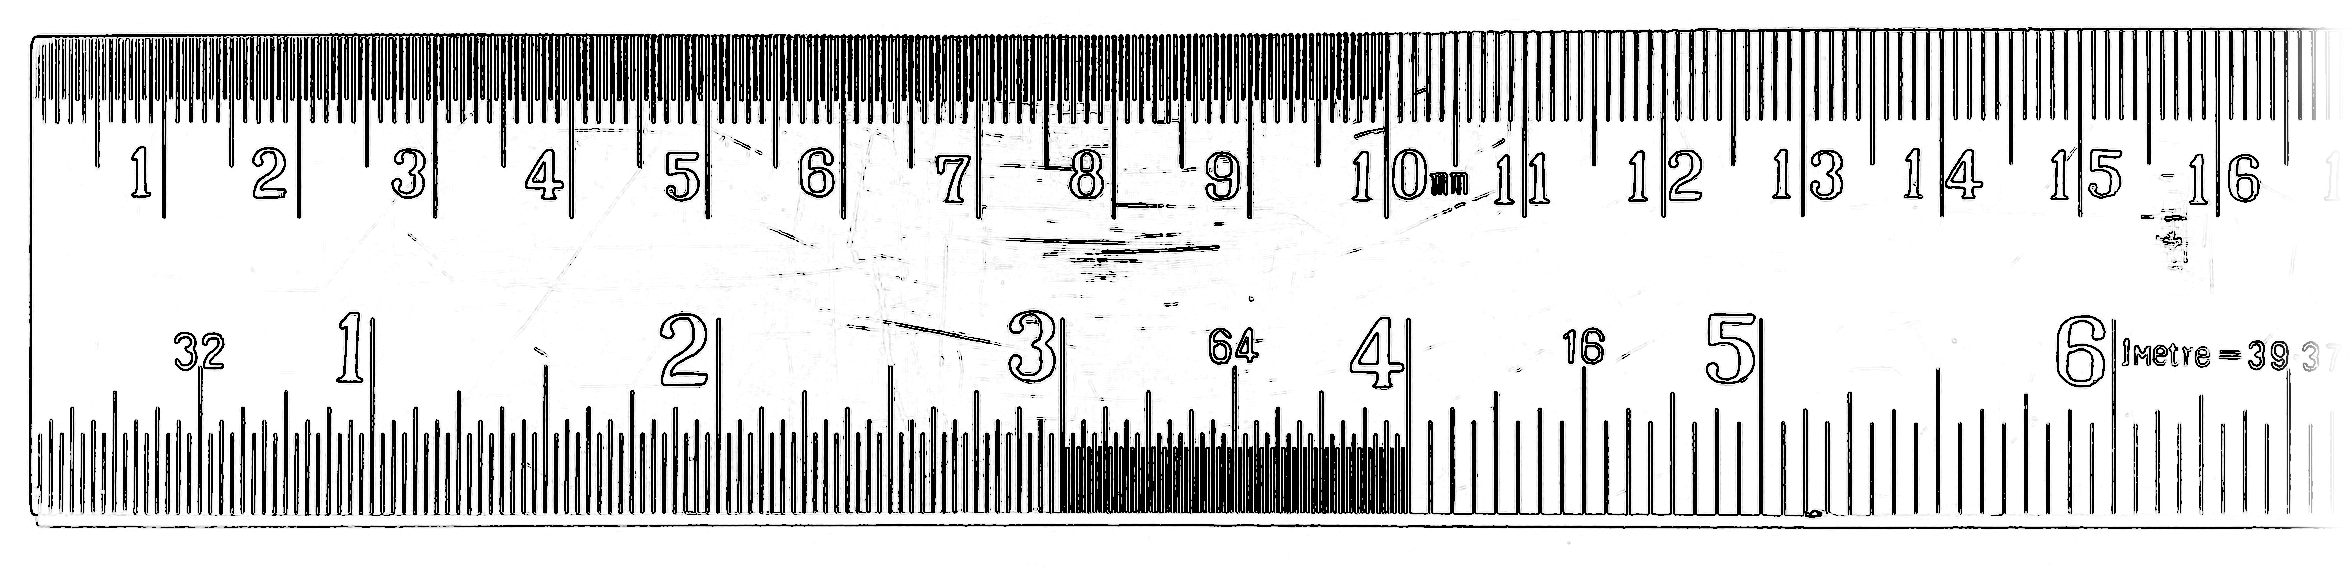
\includegraphics[width=\textwidth]{Ilustrations/Regua.png}
	\caption{Exemplo de equipamento analógico: réguas.}
\end{marginfigure}

Os equipamentos de medida podem ser divididos em dois tipos:
\begin{description}
	\item[Analógicos] Os equipamentos analógicos são aqueles que permitem que realizemos uma estimativa de valores entre duas marcas quaisquer de sua escala. São exemplos deste tipo de equipamento réguas, velocímetros de ponteiro, relógios de ponteiros, etc.

	\item[Não-analógicos] Equipamentos que não permitem a estimativa de valores são classificados como não-analógicos: nessa categoria se incluem os equipamentos digitais e aqueles dotados de escalas auxiliares. Nos equipamentos digitais, os dados da medida são mostrados através de um visor digital que permite a leitura direta dos valores numéricos\footnote[][-2cm]{Em equipamentos digitais que verificam o valor de uma quantidade que costuma sofrer pequenas variações em torno de um valor, os aparelhos geralmente realizam uma série de medidas durante um certo intervalo de tempo e mostram somente o valor médio de tais medidas. Um exemplo disso são os velocímetros digitais: devido a pequenas variações de velocidade que ocorrem durante a condução, o processo descrito acima deve ser realizado visando mostrar um número que sofra variações menos frequentes, distraindo menos o condutor.}. Já os equipamentos dotados de escala auxiliar -- também conhecida como nônio ou vernier -- possibilitam a leitura em uma escala analógica principal, porém com a leitura da subdivisão da escala principal na escala auxiliar. Como a escala auxiliar tem divisões muito ``finas'', no entanto, não é possível estimar digitos menores do que a menor divisão da escala auxiliar.
\end{description}
Vamos tratar as medidas realizadas por cada tipo de equipamento separadamente nas seções seguintes. Trataremos também a questão de \emph{algarismos significativos} de uma medida.

\begin{figure}
	\centering
	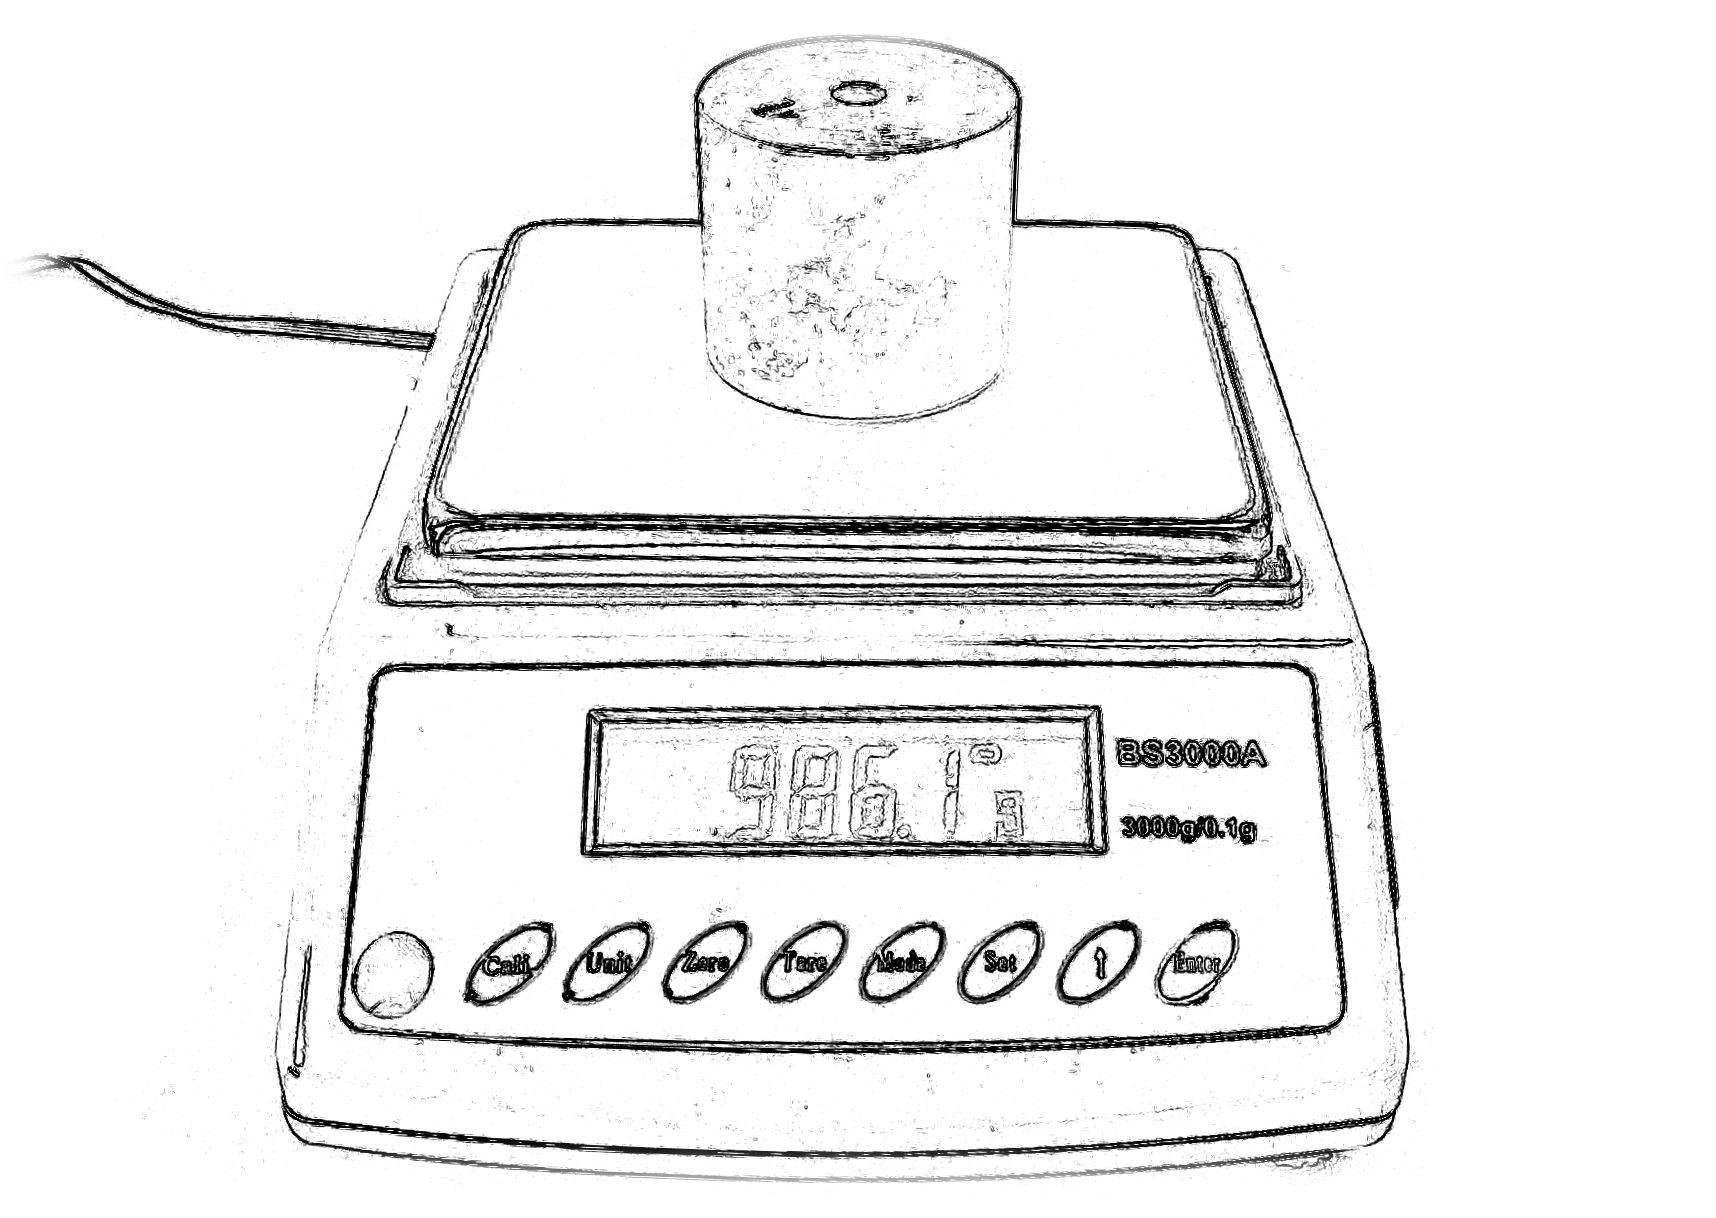
\includegraphics[width=0.7\textwidth]{Ilustrations/Balanca.png}
	\caption{Equipamentos eletrônicos geralmente utilizam um visor digital para expressar os valores medidos. Na figura, uma balança digital.}
\end{figure}
%
\begin{marginfigure}[2cm]
	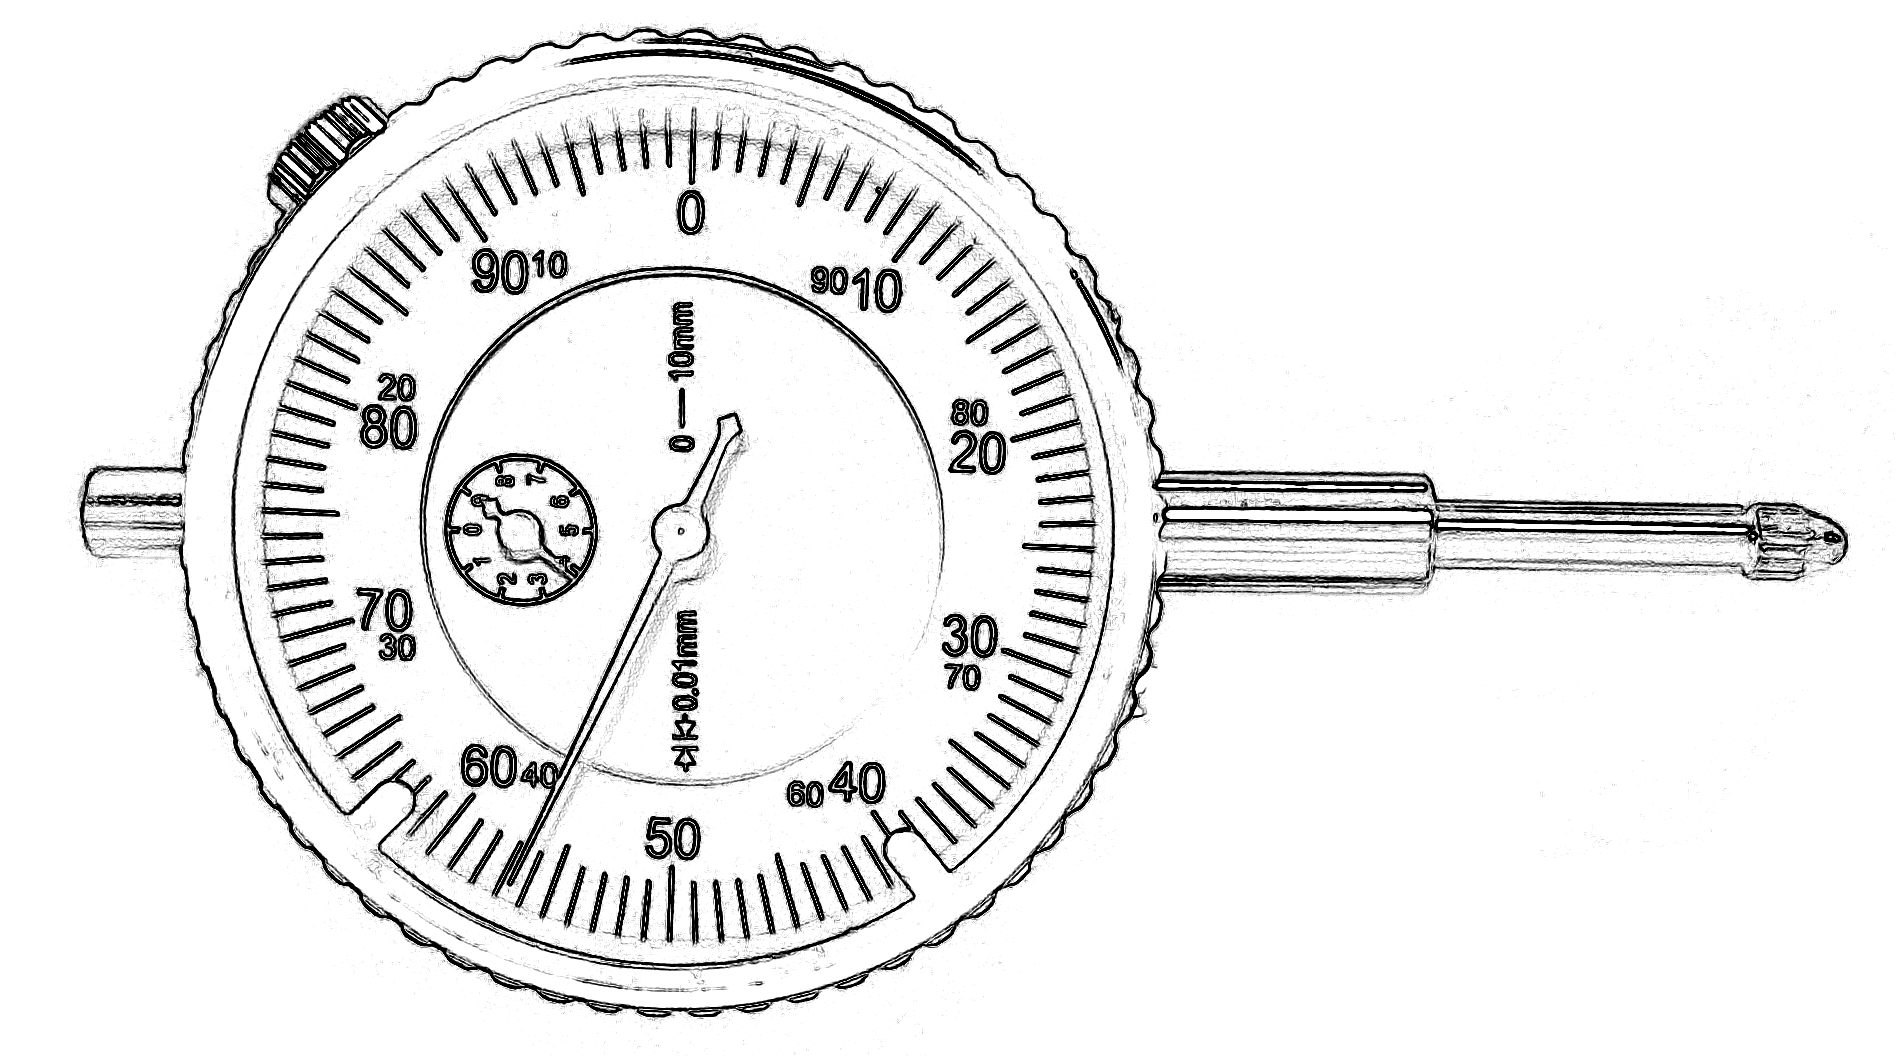
\includegraphics[width=\textwidth]{Ilustrations/Dilatometro.png}
	\caption{Equipamentos com ponteiros são exemplos comuns de equipamentos analógicos. Na figura temos um dilatômetro, equipamento utilizado para verificar pequenas variações de tamanho características de dilatação térmica (uma volta completa representa uma variação de \np[mm]{1,0}).}
\end{marginfigure}
%

%%%%%%%%%%%%%%%%%%%%%%%%%%%%%%%%%%%%%%%%%%%%%%%%%%%%%%
\subsection{Medidas realizadas com equipamentos analógicos}
\label{Sec:MedEquipAnalog}
%%%%%%%%%%%%%%%%%%%%%%%%%%%%%%%%%%%%%%%%%%%%%%%%%%%%%%

Suponhamos que precisamos usar uma trena para realizar uma medida de um muro. O equipamento em questão foi elaborado de tal forma que um metro está subdividido em 10 partes . Alinhamos uma extremidade da trena -- aquela que contém o zero -- com uma extremidade do muro e verificamos a outra extremidade. Vemos que o muro passa da marca dos 15 metros por três subdivisões, mas não passa da quarta subdivisão. O valor da medida do comprimento $\ell$ do muro está em algum ponto entre os valores correspondentes às duas marcas:
\begin{equation}
     \numprint{15,3}\textrm{~m} < \ell < \numprint{15,4}\textrm{~m}.
\end{equation}

\begin{marginfigure}[1cm]
	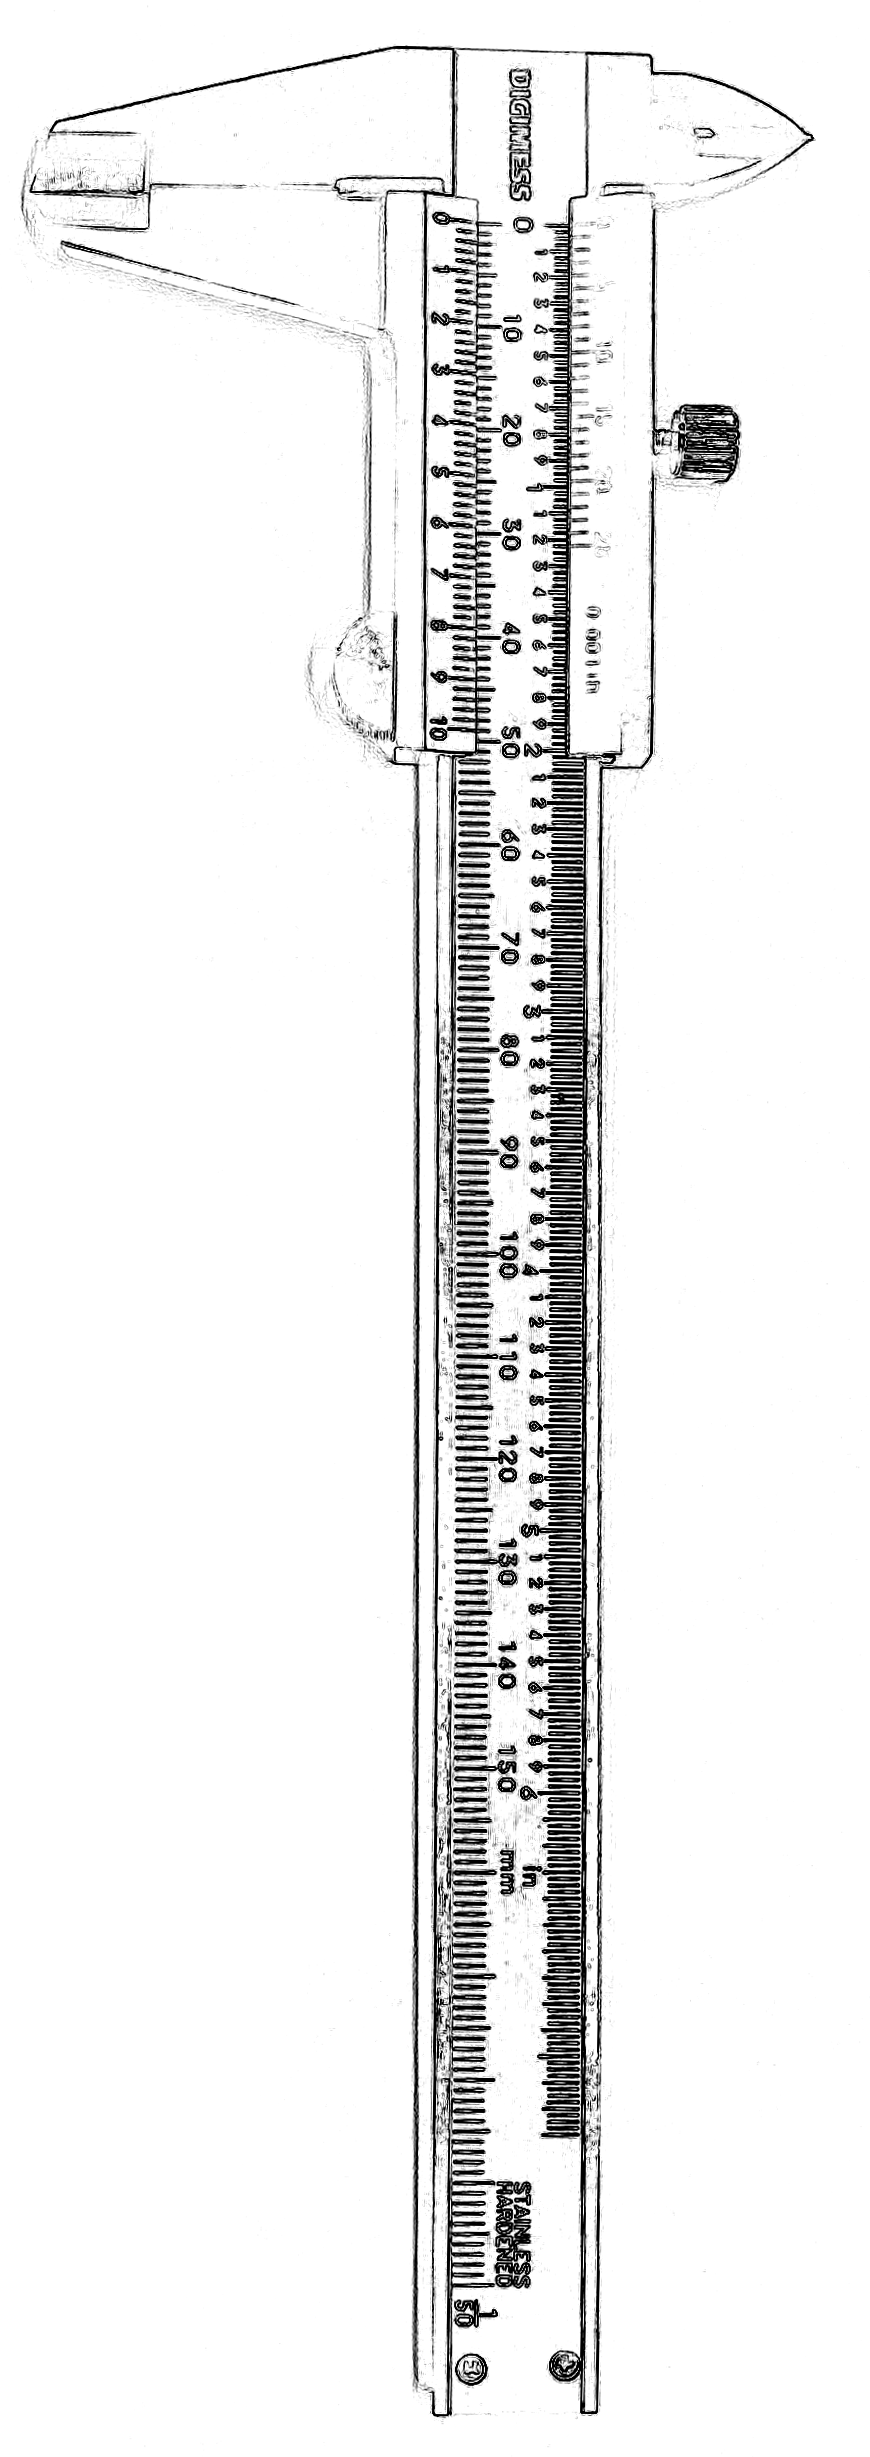
\includegraphics[width=\textwidth]{Ilustrations/Paquimetro_vert.png}
	\caption{O paquímetro é um exemplo de equipamento \emph{não-analógico}, pois é dotado de escala auxiliar (nônio).}
\end{marginfigure}

\noindent{}Sabemos que o muro termina em algum lugar entre a terceira e a quarta marca, sendo então maior que 15,3~m. Nesse caso, devemos estimar mais um algarismo. Se, por exemplo, a extremidade do muro está próxima da metade da distância entre as duas marcas da trena, porém antes dela, poderíamos estimar um valor 4 (isto é, quatro décimos da distância entre as duas subdivisões). Assim, podemos expressar a medida como,
\begin{equation}
     \ell = \numprint{15,34}\textrm{~m}.
\end{equation}

Poderíamos realizar uma estimativa com mais casas após o 4, mas a validade dela seria duvidosa: se já não temos certeza sobre a medida ser 4 (poderia ser 3 ou 5, em escalas menores é difícil efetuar uma estimativa), não temos ganho algum em denotar mais algarismos após o 4. Ao conjunto de algarismos que temos certeza (pois foram verificados no instrumento) e ao algarismo estimado, damos o nome de \emph{algarismos significativos}. O último algarismo também é conhecido como \emph{algarismo duvidoso}, pois seu valor pode mudar ao se utilizar um equipamento de medida mais preciso.

Em casos onde realizamos uma medida que coincide exatamente com uma marca, devemos considerar que o equipamento permitiria expressar divisões menores, se fosse o caso. Se, por exemplo, ao medirmos o muro com a trena mencionada a extremidade coincidir com a marca de \np[m]{15}, devemos expressar a medida como
\begin{equation}
	\ell = \np[m]{15,00},
\end{equation}
%
pois sabemos que não foi ultrapassada nenhuma submarca de décimos de metro, e determinamos que o algarismo estimado também é zero (pois se aparentemente coincide com a marca, não a ultrapassa em quantidade apreciável).

\begin{figure}
	\centering
	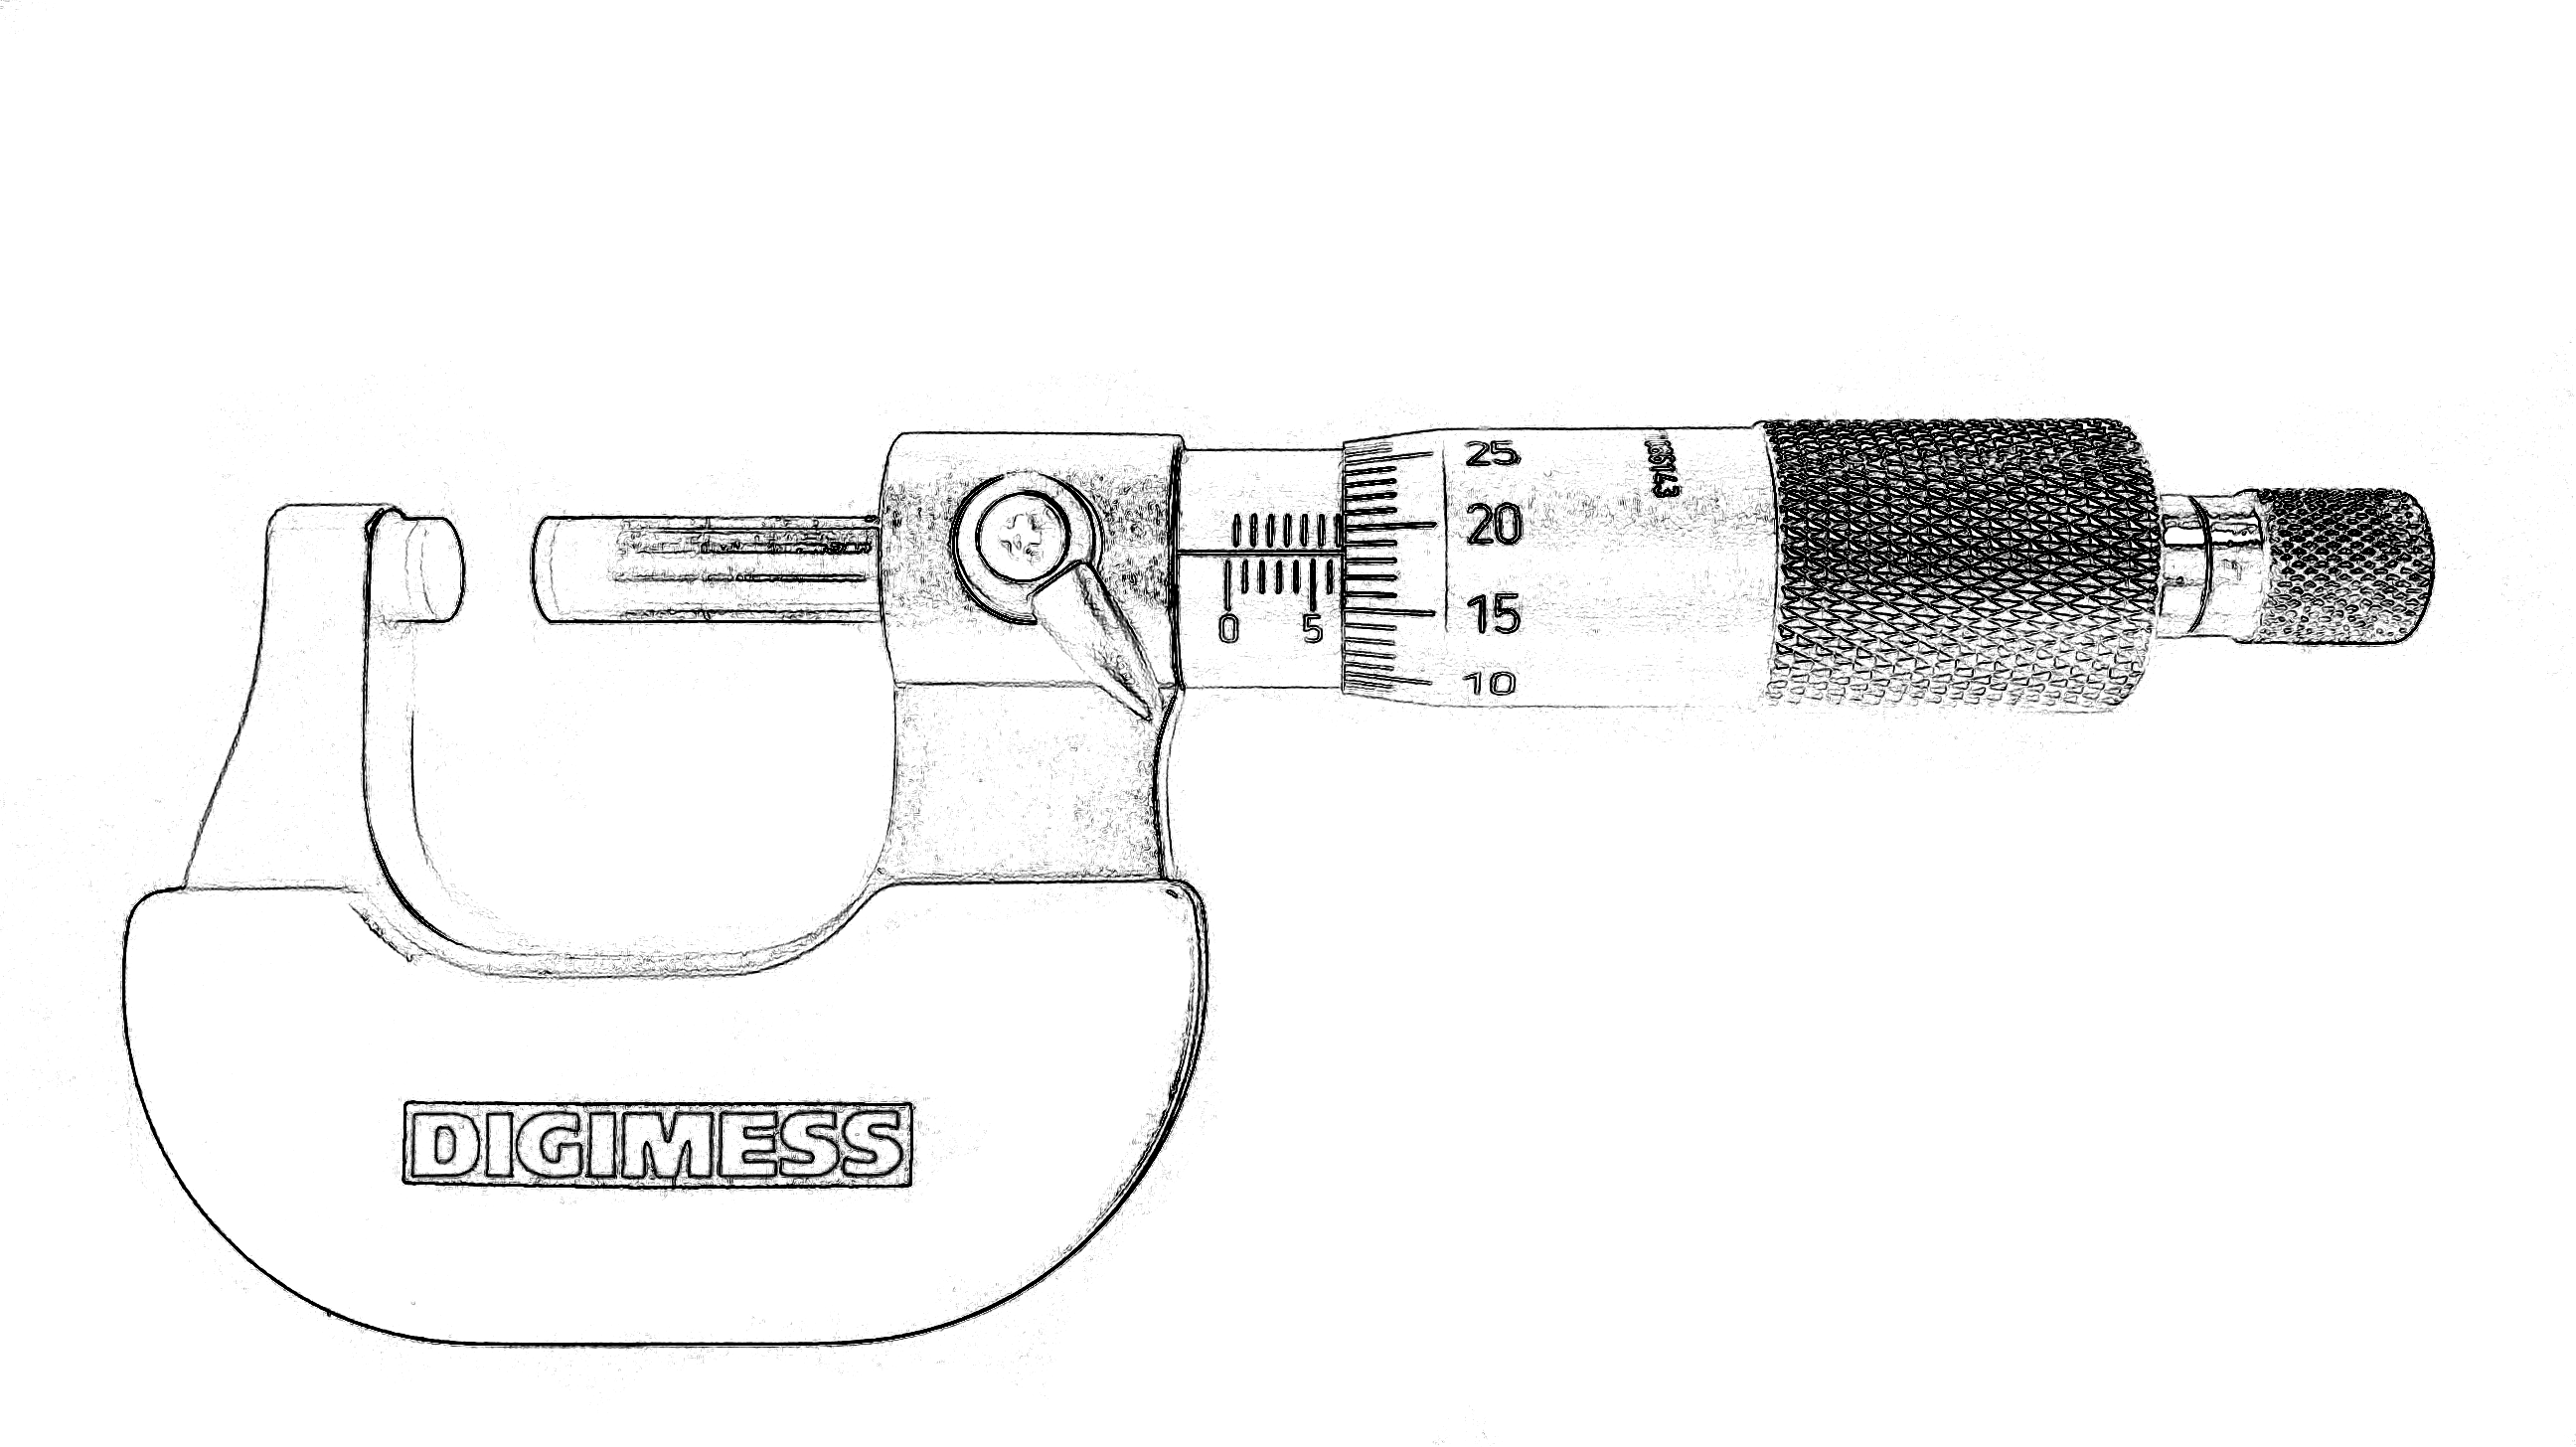
\includegraphics[width=\textwidth]{Ilustrations/Micrometro_sem_obj.png}
	\caption{Um micrômetro pode ter ou não uma escala auxiliar. Este não possui e por isso permite que um dígito seja estimado nas leituras. Os que possuem escala auxiliar tem uma série de marcas que podem se alinhar com as marcas do tambor (região numerada de 10 a 25 na figura e que pode girar), indicando a leitura apropriada para o último dígito (aquele que é estimado em um micrômetro sem escala auxiliar).}
\end{figure}

%%%%%%%%%%%%%%%%%%%%%%%%%%%%%%%%%%%%%%%%%%%%%%%%%%%%%%%%%%%%%%%
\subsection{Medidas realizadas com equipamentos não-analógicos}
%%%%%%%%%%%%%%%%%%%%%%%%%%%%%%%%%%%%%%%%%%%%%%%%%%%%%%%%%%%%%%%

No caso de equipamentos não-analógicos, podemos subdividi-los em equipamentos digitais e em equipamentos dotados de escalas auxiliares. No caso do primeiro, a medida consiste em ler os números mostrados através de um visor. Todos os algarismos mostrados são significativos --~exceto aqueles que simplesmente posicionam a vírgula, veja a seção seguinte~--. Nesse caso, o último é o algarismo duvidoso, pois, novamente, seu valor poderia ser diferente se utilizássemos um equipamento mais preciso para realizar a medida.

No caso de equipamentos dotados de escalas auxiliares, apesar de não realizarmos a leitura de um visor digital, também não realizamos estimativas. Nesse caso realizamos a leitura a partir da escala auxiliar e, devido à precisão de tal escala, não conseguimos realizar estimativas. Novamente, todos os algarismos lidos são significativos\footnote{Exceto os que posicionam a vírgula, veja a Seção~\ref{Sec:UnidadesAlgSigNotacaoCientifica} para mais informações.}, sendo que o último é denominado duvidoso devido ao fato de que pode mudar ao se utilizar um equipamento mais preciso.

\paragraph{Funcionamento da escala auxiliar}

\begin{marginfigure}[2 cm]
\centering
\begin{tikzpicture}
	
% escala principal
	\draw (0,0) -- (0,1) node[anchor=south] {0};
	\foreach \x in {0.2, 0.4, 0.6, 0.8, 1.2, 1.4, 1.6, 1.8}
		\draw (\x,0) -- (\x,0.5);
	\draw (1.0,0) -- (1.0,0.7);
	\draw (2,0) -- (2,1) node[anchor=south] {1};

% escala auxiliar
	\foreach \x [count=\xi from=0] in {0, 0.18, ..., 1.62}
		\draw (\x,-0.03) -- (\x,-0.3) node[anchor=north] {\tiny \xi};
	\draw (1.8,-0.03) -- (1.8, -0.3) node[anchor=north] {\tiny 0};
\end{tikzpicture}
\caption{Escala de um equipamento dotado de escala auxiliar. A escala superior é a principal, enquanto a inferior é a auxiliar.\label{Fig:NonioFechado}}
\end{marginfigure}


Em um equipamento dotado de uma escala auxiliar -- como um paquímetro, por exemplo --, as medidas devem ser feitas utilizando-se a posição do zero da escala auxiliar na escala principal. Na Figura~\eqref{Fig:NonioFechado} vemos uma representação das escalas de leitura típicas de um equipamento dotado de escala auxiliar: a escala maior, superior, é a principal, enquanto a menor, inferior, é a auxiliar.

A ideia por trás da escala auxiliar é bastante simples: tomamos a menor divisão da escala principal, a subdividimos em $n$ partes. Fazemos então uma escala auxiliar onde a menor divisão é a largura de $n-1$ partes. Assim se a marca do zero da escala auxiliar estiver deslocado para a direita de uma marca $i$ qualquer da escala principal pela largura da $n$-ésima parte, a marca imediatamente à direita do zero da escala auxiliar estará alinhado com a marca imediatamente à direita da $i$-ésima. Se a marca do zero estiver deslocada por duas vezes a largura da $n$-ésima parte, a segunda marca à direita do zero se alinhará à segunda marca à direita da $i$-ésima marca, e assim por diante. Dessa forma, podemos realizar uma leitura em que a menor divisão da escala é a largura da $n$-ésima parte.

\begin{marginfigure}
\centering
\begin{tikzpicture}

% escala principal
	\draw (0,0) -- (0,1) node[anchor=south] {0};
	\foreach \x in {0.2, 0.4, 0.6, 0.8, 1.2, 1.4, 1.6, 1.8}
		\draw (\x,0) -- (\x,0.5);
	\draw (1.0,0) -- (1.0,0.7);
	\draw (2,0) -- (2,1) node[anchor=south] {1};

% escala auxiliar
	\foreach \x [count=\xi from=0] in {0.02, 0.20, ..., 1.64}
		\draw (\x,-0.03) -- (\x,-0.3) node[anchor=north] {\tiny \xi};
	\draw (1.82,-0.03) -- (1.82, -0.3) node[anchor=north] {\tiny 0};
\end{tikzpicture}
\caption{Escala auxiliar deslocada para a direita por um décimo da largura da menor divisão da escala principal. Note que a marca número 1 da escala auxiliar está alinhada com a primeira marca à direita do zero da escala principal. \label{Fig:NonioAbertoUmaParte}}
\end{marginfigure}

\begin{marginfigure}
\centering
\begin{tikzpicture}

% escala principal
	\draw (0,0) -- (0,1) node[anchor=south] {0};
	\foreach \x in {0.2, 0.4, 0.6, 0.8, 1.2, 1.4, 1.6, 1.8}
		\draw (\x,0) -- (\x,0.5);
	\draw (1.0,0) -- (1.0,0.7);
	\draw (2,0) -- (2,1) node[anchor=south] {1};

% escala auxiliar
	\foreach \x [count=\xi from=0] in {0.12, 0.30, ..., 1.75}
		\draw (\x,-0.03) -- (\x, -0.3) node[anchor=north] {\tiny \xi};
	\draw (1.92,-0.03) -- (1.92, -0.3) node[anchor=north] {\tiny 0};
\end{tikzpicture}
\caption{Escala auxiliar deslocada por 6 décimos da largura da menor divisão da escala superior. Note o alinhamento da marca número 6.\label{Fig:NonioAbertoSeisPartes}}
\end{marginfigure}

Nas Figuras \ref{Fig:NonioAbertoUmaParte} e \ref{Fig:NonioAbertoSeisPartes} temos dois deslocamentos diferentes para a escala auxiliar da Figura~\ref{Fig:NonioFechado}. A escala auxiliar de tais figuras foi construída de forma que a menor divisão da escala principal foi subdividida em 10 partes. Tomando 9 partes, construímos a menor divisão da escala auxiliar. Assim, se o zero da escala auxiliar for deslocado -- em relação ao zero da escala principal -- para a direita por uma distância equivalente a um décimo da largura da menor divisão da escala principal, temos que a marca à direita do zero da escala auxiliar se alinhará à marca à direita do zero da escala principal (situação da Figura~\ref{Fig:NonioAbertoUmaParte}). Na Figura~\ref{Fig:NonioAbertoSeisPartes} o zero da escala auxiliar está deslocado em seis partes para a direita, o que leva ao alinhamento da marca número 6 da escala auxiliar com a sexta marca à direita do zero da escala principal.

\paragraph{Tomando medidas utilizando a escala auxiliar}

A Figura~\ref{Fig:NonioMedida} retrata uma medida tomada com um paquímetro cuja menor divisão da escala principal é de um milímetro e no qual a menor divisão da escala auxiliar é de 9/10 da largura da menor divisão da escala principal. Para tomar a medida, fazemos o seguinte:
%
\begin{marginfigure}
\centering
\begin{tikzpicture}

% escala principal
	\foreach \x in {-0.6, -0.4, ..., 3.2}
		\draw (\x,0) -- (\x,0.5);
	\draw (0,0) -- (0,1) node[anchor=south] {30};
	\draw (1.0,0) -- (1.0,0.7);
	\draw (2,0) -- (2,1) node[anchor=south] {40};
	\draw (3.0,0) -- (3.0,0.7);

% escala auxiliar
	\foreach \x [count=\xi from=0]in {1.12, 1.30, ..., 2.92}
		\draw (\x, -0.03) -- (\x,-0.3) node[anchor=north] {\tiny \xi};
\end{tikzpicture}
\caption{\label{Fig:NonioMedida}}
\end{marginfigure}
%
\begin{enumerate}
	\item Efetuamos a leitura na escala principal através do zero da escala auxiliar. Consideramos a marcação imediatamente à esquerda do zero da escala auxiliar. Nesse caso temos \np[mm]{35}.
	\item Verificamos qual é a marca da escala auxiliar que tem o melhor alinhamento com uma marca da escala principal. Nesse caso, temos que tal marca é a de número 6.
	\item Como dividimos a menor divisão da escala principal em 10 partes para elaborar a escala auxiliar, ao alinharmos a sexta marca da escala auxiliar, temos 6/10 de um milímetro, ou seja, \np[mm]{0,6}.
	\item Somando essas duas contribuições, temos que a medida é \np[mm]{35,6}.
\end{enumerate}
%
Veja que na prática basta \emph{ler a escala principal, colocar uma vírgula e colocar o número da marca que está alinhada}. Note ainda que o zero da direita na escala auxiliar serve para ajudar a verificar o alinhamento do zero da esquerda, pois ambos ficam alinhados ao mesmo tempo.

\begin{figure*}\forcerectofloat
\centering
\begin{tikzpicture}

% Escala principal
	\foreach \x in {0.0, 0.1, ..., 13.7}
		\draw (\x,0) -- (\x,0.5);

	\foreach \x in {0, 0.5, ..., 13.5}
		\draw (\x,0) -- (\x,0.7);

	\draw (0,0) -- (0,1) node[anchor=south] {0};
	\foreach \x in {1, 2, ..., 13}
		\draw (\x,0) -- (\x,1) node[anchor=south] {\x0};

% Escala auxiliar
	\foreach \x in {0.000, 0.098, ..., 4.9}
		\draw (\x,-0.03) -- (\x,-0.2);

	\foreach \x [count=\xi from 0] in {0, 0.490, ..., 4.9}
		\draw (\x,-0.03) -- (\x,-0.3) node[anchor=north] {\tiny \xi};
	
	\draw (4.900,-0.03) -- (4.900,-0.3) node[anchor=north] {\tiny 0};

\end{tikzpicture}
\caption{Escalas de um paquímetro milimetrado em que a menor divisão da escala principal é subdividida em 50 partes para elaborar a escala auxiliar.}
\label{Fig:Paquimetro}
\end{figure*}


\paragraph{Paquímetro com divisão de \np[mm]{1} em 50 partes}

\begin{marginfigure}[5cm]
	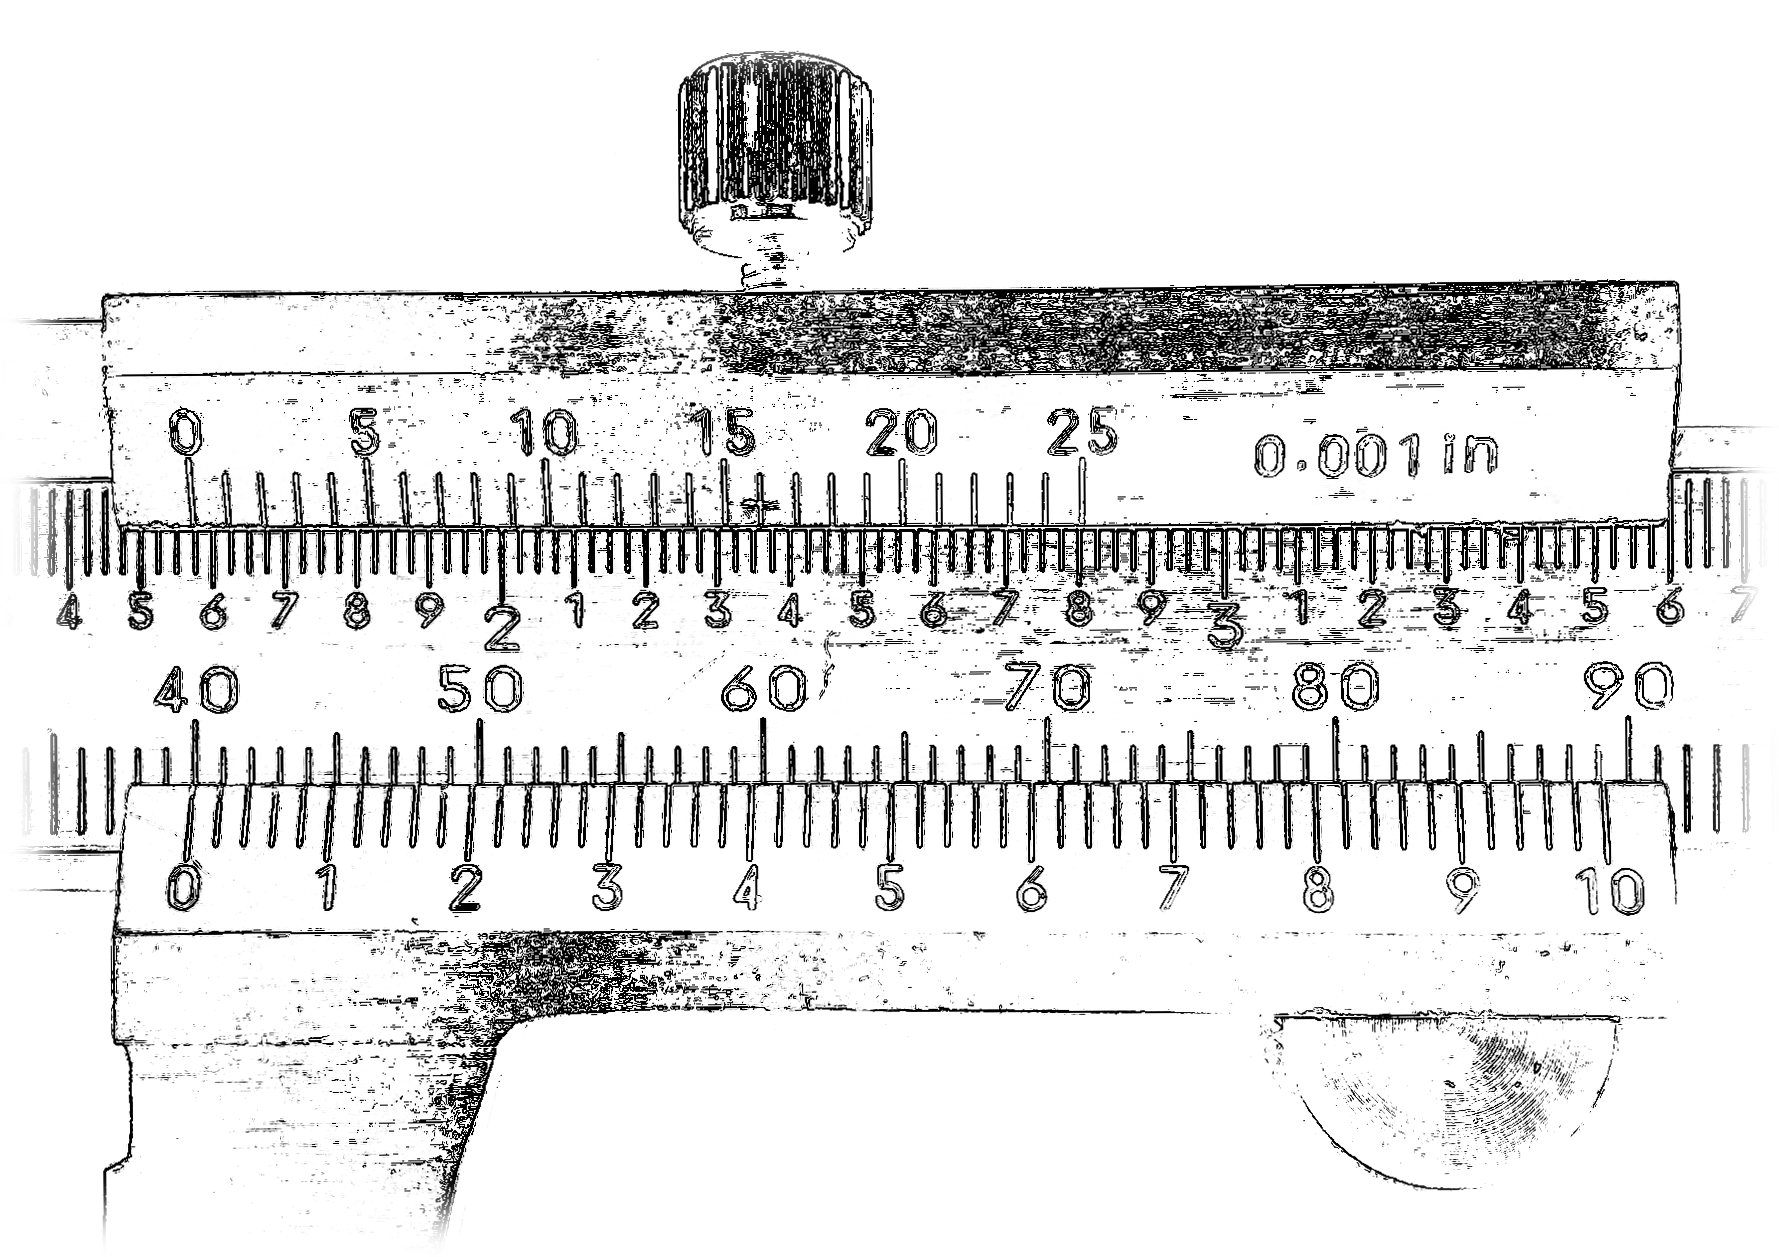
\includegraphics[width=\textwidth]{Ilustrations/Nonio.png}
	\caption{Detalhe mostrando a escala auxiliar de um paquímetro em que \np[mm]{1,0} é dividido em 50 partes.}
\end{marginfigure}

Na Figura~\ref{Fig:Paquimetro}, temos a representação das escalas de um paquímetro no qual a menor divisão da escala principal foi subdividida em 50 partes para elaborar a escala auxiliar. Portanto, verificamos que a menor divisão da escala é de \np[mm]{0,02} (1/50 de um milímetro). Se tivermos uma leitura como a da Figura~\ref{Fig:PaquimetroLeitura} em um instrumento desse tipo, procedemos a leitura através das seguintes etapas:
\begin{enumerate}
	\item Verificamos qual a leitura na escala principal da marca imediatamente à esquerda da marca do zero da escala auxiliar. Nesse caso temos \np[mm]{47}.
	\item Na escala auxiliar, procuramos a marca que está mais bem alinhada com alguma das marcas da escala principal. Em muitos casos, ficamos em dúvidas sobre qual é a marca mais bem alinhada, como duas ou três candidatas. No caso de termos três, escolha a central. No caso em questão, vemos que a primeira, a segunda e a terceira marcas à direita da marca 2 da escala auxiliar estão bem alinhadas. Escolhendo a central, temos $12 \times \np[mm]{0,02} = \np[mm]{0,24}$.
	\item A medida será composta pela soma dos dois resultados, isto é, \np[mm]{47,24}.
\end{enumerate}
%
Na prática, a leitura é bastante simples: 
\begin{enumerate}
	\item Determinamos a leitura da escala principal -- \np[mm]{47} --;
	\item Colocamos uma vírgula após o valor dessa leitura-- \np[mm]{47,} --;
	\item Verificamos a marca numerada imediatamente à esquerda da marca melhor alinhada e anotamos seu dígito -- \np[mm]{47,2} --; \hyphenation{mul-ti-pli-ca-mos}
	\item Finalmente, verificamos a posição da marca melhor alinhada a partir da última numerada -- nesse caso, a segunda posição --. Como cada marca da escala auxiliar corresponde a \np[mm]{0,02}, ``multiplicamos'' por dois o ``valor'' da posição e anotamos o resultado ao fim --~\np[mm]{47,24}~--.
\end{enumerate}

\begin{figure*}
\centering
\begin{tikzpicture}

% Escala principal
	\foreach \x in {0.0, 0.1, ..., 13.7}
		\draw (\x,0) -- (\x,0.5);

	\foreach \x in {0, 0.5, ..., 13.5}
		\draw (\x,0) -- (\x,0.7);

	\draw (0,0) -- (0,1) node[anchor=south] {0};
	\foreach \x in {1, 2, ..., 13}
		\draw (\x,0) -- (\x,1) node[anchor=south] {\x0};

% Escala auxiliar
\begin{scope}[xshift=4.724cm]
	\foreach \x in {0.000, 0.098, ..., 4.9}
		\draw (\x,-0.03) -- (\x,-0.2);

	\foreach \x [count=\xi from 0] in {0, 0.490, ..., 4.9}
		\draw (\x,-0.03) -- (\x,-0.3) node[anchor=north] {\tiny \xi};
	
	\draw (4.900,-0.03) -- (4.900,-0.3) node[anchor=north] {\tiny 0};
\end{scope}
\end{tikzpicture}
\caption{Leitura de \np[mm]{47,24}. Note o entre alinhamento a segunda marca após a marca ``2'' na escala auxiliar e a marca da escala principal.\label{Fig:PaquimetroLeitura}}
\end{figure*}

Uma observação importante ao se utilizar equipamentos dotados de escala auxiliar é a realização de medidas que coincidem com as marcas maiores da escala auxiliar. Na Figura~\ref{Fig:PaquimetroLeituraZero}, por exemplo, tempos uma medida em que a marca da escala auxiliar que está alinhada à da escala principal é a denotada pelo número 2. Efetuando a leitura, temos \np[mm]{33,2}. No entanto, temos o último dígito, dado pela ``posição'' da marca alinhada ``multiplicada'' por dois. Se a marca alinhada é a numerada, então a posição é zero. Logo, devemos adicionar um zero ao final da medida: \np[mm]{33,20}. Uma maneira mais simples de interpretar essa questão é verificarmos que o número de algarismos após a vírgula em uma dada unidade para um instrumento qualquer é sempre o mesmo. Assim, temos que no caso do paquímetro dos exemplos acima o número é sempre de duas casas após a vírgula ao se efetuar medidas em milímetros.
\begin{figure*}
\centering
\begin{tikzpicture}

% Escala principal
	\foreach \x in {0.0, 0.1, ..., 13.7}
		\draw (\x,0) -- (\x,0.5);

	\foreach \x in {0, 0.5, ..., 13.5}
		\draw (\x,0) -- (\x,0.7);

	\draw (0,0) -- (0,1) node[anchor=south] {0};
	\foreach \x in {1, 2, ..., 13}
		\draw (\x,0) -- (\x,1) node[anchor=south] {\x0};

% Escala auxiliar
\begin{scope}[xshift=3.320cm]
	\foreach \x in {0.000, 0.098, ..., 4.9}
		\draw (\x,-0.03) -- (\x,-0.2);

	\foreach \x [count=\xi from 0] in {0, 0.490, ..., 4.9}
		\draw (\x,-0.03) -- (\x,-0.3) node[anchor=north] {\tiny \xi};
	
	\draw (4.900,-0.03) -- (4.900,-0.3) node[anchor=north] {\tiny 0};
\end{scope}
\end{tikzpicture}
\caption{Leitura de \np[mm]{33,20}. Note o entre alinhamento a  marca ``2'' na escala auxiliar e a marca da escala principal.\label{Fig:PaquimetroLeituraZero}}
\end{figure*}
%A invenção da escala auxiliar ... \comment{fazer}

%%%%%%%%%%%%%%%%%%%%%%%%%%%%%%%%%%%%%%%%%%%%%%%%%%%%%%%%%%%%%%%%%%%%%
\subsection{Unidades e algarismos significativos, notação científica}
\label{Sec:UnidadesAlgSigNotacaoCientifica}
%%%%%%%%%%%%%%%%%%%%%%%%%%%%%%%%%%%%%%%%%%%%%%%%%%%%%%%%%%%%%%%%%%%%%

O número de algarismos significativos de uma medida está ligado à precisão do equipamento utilizado para realizá-la. Devido a isso, se realizarmos uma conversão de unidades, não podemos ter uma alteração no número de algarismos significativos -- afinal a precisão não aumenta nem diminui~--. Isso nos leva a contemplar as duas seguintes situações:
\begin{enumerate}
\item Realizarmos uma medida e obtemos
\begin{equation}
	\ell = \np[mm]{34,82},
\end{equation}
%
onde o último algarismo foi estimado. Sabemos que temos quatro algarismos significativos e ao expressarmos esta medida em outras unidades, devemos manter o mesmo número de algarismos significativos. Podemos então expressá-la como
\begin{align}
	\ell &= \np[cm]{3,482} \\
	&= \np[dm]{0,3482} \\
	&= \np[m]{0,03482}.
\end{align}
%
Note que os zeros à esquerda não são algarismos significativos. Sua função é exclusivamente a de posicionar a vírgula, dando aos algarismos a ordem de grandeza adequada.

\item Realizamos uma medida de massa obtemos,
\begin{equation}
	m = \np[kg]{11,2},
\end{equation}
%
e desejamos expressá-la em gramas. Efetuando a conversão, poderíamos escrever em um primeiro momento
\begin{equation}
	m = \np[g]{11200}.
\end{equation}
%
Uma medida assim expressa, no entanto, tem cinco algarismos significativos -- pois o último algarismo anotado é o duvidoso --, enquanto a medida original tem três.  Portanto, por mais que possamos adicionar zeros ao lado esquerdo sem modificar o número de significativos, não podemos fazê-lo do lado direito. 

Para expressar essa medida com o número adequado de algarismos significativos, podemos utilizar a notação científica. Um número expresso em notação científica tem a forma $a \cdot 10^b$, onde $a$ -- denominada \emph{mantissa} -- é um número Real --, e $b$ -- o expoente -- é um número inteiro. O expoente também é conhecido como \emph{ordem de grandeza}. Em um número expresso dessa forma, somente os algarismos da mantissa são significativos. Os prefixos kilo (k), hecto (h), deci (d), centi (c), mili (m), micro ($\mu$), nano (n), etc., utilizados em unidades de medida são simplesmente formas abreviadas para as notações $\cdot 10^{3}$, $\cdot 10^{2}$, $\cdot 10^{-1}$, $\cdot 10^{-2}$, $\cdot 10^{-3}$, $\cdot 10^{-6}$, $\cdot 10^{-9}$, etc.

Utilizando a notação científica temos então
\begin{equation}
	m = \np[g]{112e2}.
\end{equation}
\end{enumerate}

Portanto, temos as seguintes regras:
\begin{itemize}
	\item Conversões de unidade não alteram a precisão das medidas e por isso não podem alterar o número de algarismos significativos.
	\item Zeros à esquerda não contam como algarismos significativos.
	\item Não podemos adicionar zeros à direita. Se for necessário fazê-lo ao efetuar uma conversão de unidades, devemos utilizar a notação científica.
\end{itemize}

%%%%%%%%%%%%%%%%%%%%%%%%%%%%%%%%%%%%%%%%%%%%%%%%%%%%%%%%%%
\subsection{Operações envolvendo medidas}
%%%%%%%%%%%%%%%%%%%%%%%%%%%%%%%%%%%%%%%%%%%%%%%%%%%%%%%%%%

Lembre-se que em uma medida direta, o algarismo duvidoso está ligado à ideia de que ele seria o algarismo que possivelmente sofreria alterações caso utilizássemos equipamentos mais precisos para realizar as medidas. Isso também se reflete nos valores calculados para medidas indiretas, afinal elas são calculadas a partir de medidas diretas, que têm um algarismo duvidoso. Portanto, ao obtermos uma medida indireta, também devemos denotá-la com o número adequado de algarismos significativos.

Para determiná-los, no entanto, devemos seguir algumas regras para as operações realizadas:
\begin{description}
	\item[Multiplicação e divisão] No caso da multiplicação ou da divisão, devemos limitar o número de algarismos significativos àquele da medida que tiver o menor número.
	
	Para entender a razão dessa regra, podemos fazer a seguinte análise: Tomamos a medida indireta $L$ dada por
\begin{equation}
	L = \ell_1\ell_2\ell_3\dots
\end{equation}
%
onde $\ell_1$, $\ell_2$, $\ell_3$, \dots, são medidas diretas quaisquer. Vamos supor que $\ell_1$ tem $n$ algarismos significativos e que as demais têm mais algarismos significativos que $\ell_1$. Vamos supor ainda que o primeiro dígito (aquele com a maior ordem de grandeza) tem ordem de grandeza $p$, que o duvidoso ordem de grandeza $d$ e que a diferença entre as ordens de grandeza desses dígitos é $s$. Agora fazemos o seguinte
		\begin{enumerate}
			\item Tomamos a ordem de grandeza $d$ do algarismo duvidoso de $\ell_1$ e multiplicamos pelas demais medidas;
			\item Obtemos um valor com uma ordem de grandeza $d'$ qualquer;
			\item Qualquer dígito com uma ordem de grandeza menor que $d'$ é então desprezível se comparado ao dígito com a ordem de grandeza $d$;
			\item Observamos no valor calculado para $L$ que o dígito com a maior ordem de grandeza será $p'$. Esse dígito deve ser $s'$ ordens de grandeza maior que $d'$.
		\end{enumerate}
%
A diferença $s'$ nada mais é do que o número de algarismos significativos da medida $L$. Além disso $s'$ é igual a $s$. Logo, o resultado deve ter o mesmo número de algarismos significativos que a medida $\ell_1$. Portanto, ao multiplicar duas ou mais medidas,
	\begin{itemize}
		\item Determinamos o número de algarismos significativos de cada uma das medidas que compõe o produto/divisão;
		\item Realizamos o produto/divisão;
		\item Ao fim, deixamos o resultado com o mesmo número de algarismos significativos que a medida que tem menos algarismos significativos.
	\end{itemize}
	
	Uma observação importante a se fazer é que se separarmos o cálculo em várias etapas, devemos levar mais algarismos do que o mínimo necessário entre as etapas (pelo menos um a mais). A razão disso é que a contribuição dos dígitos após o último significativo pode se acumular entre as etapas e dar um resultado levemente maior que no caso de os descartarmos. O descarte dos algarismos não-significativos deve ser feito ao final do cálculo.
		
	\textsc{Exemplo}\footnote{Utilizamos a barra para denotar o último algarismo significativo quando escrevemos dígitos além dele.}:
\begin{subequations}\label{Eq:AlgarismosSignificativosMult}
\begin{align}
     \numprint{12,03} \div \numprint{3,6} &= 3,\overline{3}4 = \numprint{3,3} \\
     \numprint{198,633} \times \numprint{3,211} &= 637,\overline{8}1056 = \numprint{637,8}.
\end{align}
\end{subequations}

	\item[Soma e subtração] Para o caso da soma ou subtração, mantemos o número de casas decimais da medida que tem o menor número de casas após a vírgula. 
	
	A razão disso é que se temos uma incerteza em um algarismo qualquer, dígitos à direita serão menores ou da ordem de grandeza da incerteza. Consequentemente, sería inútil expressá-los. Observe que para realizar a soma/subtração, é importante que todas as medidas sejam expressas na mesma unidade e ordem de grandeza.
	
	\textsc{Exemplo:}
\begin{align}
	 \numprint[cm]{12,03} + \numprint[cm]{3,6} &= 15,\overline{6}3~\textrm{cm}\\
		 &= \numprint[cm]{15,6}.
\end{align}

	\item[Constantes] Quando efetuamos uma operação envolvendo uma constante matemática e uma medida, conservamos no resultado o mesmo número de algarismos significativos da medida. 
	
	Nesse caso temos que a constante matemática não tem incerteza nenhuma, então podemos considerá-la com um número infinito de algarismos significativos.
	
	\textsc{Exemplo:}
\begin{align}
	A &= \pi \times (3,66~\textrm{m})^2 \\
	  &= \pi \times (13,\overline{3}956~\textrm{m}^2)\\
	  &= 42,\overline{0}8351855~\textrm{m}^2 \\
	  &= \numprint{42,1}~\textrm{m}^2.
\end{align}

\item[Funções] Quando uma medida é o argumento de uma função, mantemos para o resultado o número de algarismos significativos da medida. 

Uma maneira de entender isso é o fato de que podemos escrever funções como séries de potência\footnote{Uma série de potência é uma forma de escrever uma função em termos de potências, somas e subtrações. Em geral, tais séries contém um número infinito de termos.

As funções trigonométricas $\sen x$ e $\cos x$, por exemplo, são descritas pelas séries
\begin{align*}
	\sen x = x - \frac{x^3}{3!} + \frac{x^5}{5!} - \frac{x^7}{7!} + \dots \\
	\cos x = 1 - \frac{x^2}{2!} + \frac{x^4}{4!} - \frac{x^6}{6!} + \dots,
\end{align*}
%
onde $x$ é um ângulo expresso em radianos.
} -- que são basicamente multiplicações, somas e subtrações~--. Dessa forma, podemos verificar que ao tomarmos a medida e realizarmos o produto por ela mesma, devemos ter um resultado com o mesmo número de algarismos significativos para todas as parcelas que serão somadas/subtraídas, sendo que o número de casas após a vírgula fica determinado pelo primeiro termo que não é constante. Assim, ao somarmos, a parcela maior dominará e teremos que o resultado terá o mesmo número de algarismos significativos que o argumento da função\footnote{Isso é útil para podermos truncar a soma da série a um número pequeno de parcelas, afinal não faz sentido calcular parcelas que têm valores menores que a incerteza das parcelas dominantes}.

\textsc{Exemplo:}
\begin{align}
	x &= \ln \numprint{3,555} \\
	&= 1,26\overline{8}355063 \\
	&= 1,268.
\end{align}
\end{description}

%%%%%%%%%%%%%%%%%%%%%%%%%%%%%
\subsection{Arredondamento}
%%%%%%%%%%%%%%%%%%%%%%%%%%%%%

Nos exemplos da seção anterior, usamos uma barra para denotar o último algarismo significativo antes de descartar os algarismos excedentes. Sempre que os descartarmos, devemos fazê-lo observando os critérios de arredondamento.

Quando obtemos resultados do tipo
\begin{equation}
     \ell = 134,\overline{3}9487,
\end{equation}
%
precisamos fazer um \emph{arredondamento}. No exemplo acima, vemos que 134,4 é um número mais próximo do resultado do que 134,3. Portanto, adotamos as seguintes regras ao realizarmos o arredondamento:
\begin{enumerate}
     \item Se o algarismo seguinte ao duvidoso for menor que 5, simplesmente descartamos os algarismos excedentes.
     \item Se o algarismo seguinte ao duvidoso for maior ou igual a 5, aumentamos o duvidoso de uma unidade e descartamos os demais.
\end{enumerate}
%
Esse critério de arredondamento não é único. Em algumas situações se utiliza uma regra específica para o caso de o algarismo seguinte ao duvidoso ser 5: analisa-se o algarismo seguinte a esse e caso ele for par, se arredonda para cima e caso for ímpar, para baixo.


\chapter{Gráficos}
\label{Chap:Graficos}

\begin{fullwidth}
{\it
Uma maneira simples de verificar a relação entre duas grandezas é a elaboração de um gráfico de dispersão. Apesar de não podermos verificar valores exatos em um gráfico, uma observação do comportamento geral de um conjunto de pontos pode ser muito esclarecedora, principalmente se levarmos em conta que todas as medidas efetuadas sofrem uma dispersão aleatória em torno de seus valores ideais. Verificaremos como elaborar um gráfico de maneira a evidenciar o comportamento das variáveis consideradas e, no Capítulo~\ref{Chap:RegressoLinear}, verificaremos como descrever de maneira idealizada a dependência entre as variáveis.
}
\end{fullwidth}

%%%%%%%%%%%%%%%%%%
\section{Gráficos}
%%%%%%%%%%%%%%%%%%

Um gráfico é uma maneira de transformar um conjunto de dados numéricos em uma figura, relacionando valores numéricos a escalas de cor, distâncias ou áreas. No livro \emph{The Visual Display of Quantitative Information}\cite{Tufte2001}, Edward R. Tufte
afirma que
\begin{quote}
	Gráficos mostram quantidades visualmente através do uso combinado de pontos, linhas, um sistema de coordenadas, números, símbolos, palavras, sombreamento, e cor.
\end{quote}
%
e que
\begin{quote}
	Gráficos modernos podem fazer muito mais que simplesmente substituir pequenas tabelas de dados. Quando utilizados em seu máximo potencial, gráficos são instrumentos para raciocinar sobre informações quantitativas. Frequentemente a maneira mais efetiva para descrever, explorar, e sumarizar um conjunto de números ---~mesmo um conjunto muito grande~--- é através de figuras de tais números.
\end{quote}

Tufte afirma que talvez em virtude da diversidade de técnicas e informações necessárias ---~habilidades artísticas e matemáticas, dados experimentais~--- a utilização de figuras abstratas para representar números é relativamente recente (1750 em diante). Dentre os autores que desenvolveram o campo da representação gráfica de dados, ele destaca o trabalho de William Playfair, que desenvolveu melhorias para vários tipos de gráficos. Tufte também destaca do trabalho de Johann Heinrich Lambert,bib que percebe que os gráficos não precisam necessariamente relacionar quantidades em analogia ao mundo físico ---~como séries temporais, isto é, a evolução de um valor qualquer de acordo com a evolução do tempo~---, mas podem ser elaborados para quaisquer duas variáveis cujas relações desejamos verificar:

\begin{quote}
	Temos em geral duas quantidades variáveis, $x$, $y$, que serão comparadas uma à outra por observação, de forma que para cada valor de $x$ ---~que pode ser considerada como uma abscissa~--- determinamos a ordenada correspondente $y$. Se as observações experimentais fossem completamente precisas, essas ordenadas resultariam em um número de pontos através dos quais uma curva ou uma reta deveriam ser traçadas. \cite{Lambert}
\end{quote}

Existem vários tipos de gráficos, cada um com o objetivo de evidenciar características específicas do conjunto de dados em questão:
\begin{itemize}
	\item \emph{Gráficos de setores} servem bem o propósito de mostrar a contribuição relativa de várias parcelas que perfazem um todo;
	\item \emph{Gráficos de colunas/barras} servem para comparação entre diversos valores absolutos;
	\item \emph{Gráficos de colunas/barras empilhadas} denotam valores absolutos e demonstram a composição relativa de várias contribuições para o todo. Une as propriedades dos dois tipos anteriores;
	\item \emph{Séries temporais} denotam a evolução temporal de variáveis com o tempo;
	\item \emph{Mapas de dados} servem para demonstrar dados que variam de acordo com a distribuição geográfica;
	\item \emph{Gráficos de dispersão} permitem verificar a relação entre duas variáveis quaisquer;
	\item \emph{Histogramas} são similares aos gráficos de barra, mas voltados à apresentação de contagens de eventos em diversos intervalos;
	%\item \emph{Gráficos de radar}
	%\item \emph{Gráficos de curva de nível}
\end{itemize}
%
além de outros tipos. Em comum a todos os tipos de gráfico, está a utilização de dimensões como área e comprimento, ou tonalidades de cor, para representar informações numéricas.

Temos especial interesse nos gráficos de dispersão. Esse tipo de gráfico serve para verificar relações de causa e efeito entre duas variáveis quaisquer. De acordo com Tufte,
\begin{quote}
	[...] Na literatura científica moderna, em torno de 40\% dos gráficos publicados têm uma forma relacional, com duas ou mais variáveis. Isto não é sem propósito, já que os gráficos relacionais ---~em sua forma mais simples, o gráfico de dispersão e suas variantes~--- é o mais formidável de todos os tipos de gráficos. Eles ligam pelo menos duas variáveis, encorajando e mesmo suplicando que o leitor se pergunte qual é a possível relação causal entre elas. Eles confrontam as teorias causais [...] com evidências empíricas.
\end{quote}
%
De fato, estamos interessados em verificar experimentalmente a relação entre diversas variáveis através de experimentos. Além disso, desejamos testar teorias científicas, procurando confirmar ou refutar suas validades.

Finalmente, como recomendações gerais para a elaboração de gráficos, Tufte destaca:
\begin{itemize}
	\item \emph{A representação de números através de medidas de superfície em um gráfico deve ser proporcional às quantidades numéricas representadas}. \footnote[][-3cm]{Esse item é bastante visível ao se analisar um gráfico de campanha política: o candidato que deseja evidenciar sua vantagem costuma realizar um corte de forma que o zero não seja no menor valor da escala mostrada e também adota uma largura maior para sua coluna. Dessa forma uma diferença insignificante (menor que o erro da própria pesquisa) parece muito grande.}
	\item \emph{Cada parte de um gráfico gera expectativa visual sobre as outras partes. Se uma escala que se move em intervalos regulares, por exemplo, se espera que ela continue a fazê-lo. Mostre a variação dos dados, não variação na elaboração do gráfico.}
	\item \emph{Em séries temporais, ao se mostrar dados relativos a dinheiro, geralmente é melhor utilizar quantidades corrigidas pela inflação}.
	\item \emph{O número de dimensões utilizadas para demonstrar informações não deve exceder o número de dimensões dos dados}\footnote{As dimensões são as maneiras diferentes que os dados podem variar. Se, por exemplo, desejamos comparar o número de habitantes de diversas cidades, devemos utilizar uma figura com uma dimensão (um gráfico de barras) e não com duas (a área de um círculo).}.
	\item \emph{Acima de tudo, mostre os dados.}\footnote{Isto é, faça um gráfico simples, sem floreios, que mostre os dados.}
\end{itemize}


%%%%%%%%%%%%%%%%%%%%%%%%%%%%%%%%%%
\section{Gráficos de dispersão}
%%%%%%%%%%%%%%%%%%%%%%%%%%%%%%%%%%

Gráficos de dispersão são ferramentas muito usadas para visualizar relações matemáticas entre uma função e seu argumento. Por exemplo, sabemos que a função $f(x) = A + Bx$ é uma equação da reta, pois seu gráfico é uma reta. Cada função tem um gráfico característico. 

Em experimentos de laboratório é comum procuramos estabelecer a relação entre duas grandezas. Uma delas variamos arbitrariamente e denominamos como \textbf{variável independente}, já a outra medimos e ---~como seus valores variam em resposta aos da variável independente~--- a denominamos como \emph{variável dependente}. Tais variáveis são representadas nos eixo $x$  (abscissas) e $y$ (ordenadas), respectivamente, sendo o primeiro o eixo horizontal e o segundo o vertical. É comum nos referirmos a um gráfico como sendo do tipo $\Delta x \times t$, $\Delta L \times \Delta T$, etc. ---~ou ainda $\Delta x \;vs\; t$, $\Delta L \;vs\; \Delta T$, etc.~---. Nessa notação, a variável à esquerda do símbolo $\times$, ou do $vs$ (\emph{versus}), denota a quantidade que corresponde ao eixo vertical, enquanto o símbolo à direita denota a variável que corresponde ao eixo horizontal.

O maior objetivo de uma teoria é justamente encontrar a relação matemática $f$ que relaciona $x$ e $y$, ou seja, que nos dá $y$ \emph{em função de} $x$: $y = f(x)$. Isso não é algo que possa ser retirado dos gráficos de uma maneira simples, por diversas razões. Primeiramente, os dados experimentais se distribuem em torno do comportamento ideal devido a variações aleatórias. Além disso, mesmo que possamos tirar uma conclusão a partir do gráfico, tal conclusão só é válida para o intervalo de valores que compreende as medidas, podendo ser diferente em outras regiões. Finalmente, uma relação extraída dos dados experimentais não consegue explicar em argumentos lógicos o mecanismo que relaciona uma variável à outra, portanto não explicando o comportamento. De qualquer forma, uma gráfico que mostra uma dependência confiável de uma variável em relação a outra já abre um caminho para a investigação. Também podemos utilizar os dados experimentais para \emph{verificar a validade de previsões teóricas}.

\pagebreak
%%%%%%%%%%%%%%%%%%%%%%%%%%%%%%%%%%%%%%%%%%%%%%%%%%%%%%%%%%%%%%%
\subsection{Principais elementos de um gráfico de dispersão}
%%%%%%%%%%%%%%%%%%%%%%%%%%%%%%%%%%%%%%%%%%%%%%%%%%%%%%%%%%%%%%%

Os elementos mais notáveis de um gráfico de dispersão são:
\begin{description}
	\item[Eixos:] Os valores das variáveis dependente e independente  são expressos pelas distâncias ao longo dos eixos vertical e horizontal em relação à origem (encontro dos dois eixos). Muitas vezes os valores das variáveis são distantes de zero e não podem ser verificados adequadamente se um dos eixos ---~ou mesmo ambos~--- iniciarem em zero. Por isso, é comum que se realizem ``cortes'' nos eixos de maneira que eles não iniciem em zero. Nesse caso, os valores são expressados por meio da distância relativa que os pontos ocupam entre duas marcas numeradas nos eixos (veja o item seguinte). Os eixos devem ser nomeados com a variável que está sendo representada e suas unidades.
	\item[Escalas:] Para que a leitura do gráfico possa ser efetuada de uma maneira quantitativa, ainda que aproximada, é importante que se efetuem marcas nos eixos e que tais marcas sejam numeradas com os valores que elas representam no eixo. Tais marcas não precisam iniciar em zero, porém devem ser efetuadas em intervalos regulares e com números de fácil leitura. Nas escalas não devem ser marcados os valores das abscissas e ordenadas dos pontos\footnote{Exceto no caso em que os próprios valores das variáveis ocorrem em intervalos regulares e tais intervalos correspondem ao mais adequado para a escala do eixo. Isso ocorre mais comumente com os valores do eixo independente (horizontal).}.
	\item[Pontos experimentais:] Os dados experimentais são representados através de pontos na área retangular delimitada pelos eixos horizontal e vertical. A localização dos pontos é aquela do encontro das retas paralelas aos eixos horizontal e vertical e que passam pelas posições desses eixos que correspondem aos valores que desejamos representar. Para que o ponto seja facilmente visível, indica-se a utilização de quadrados, círculos, triângulos, etc. centrados no ponto de encontro das retas. Caso mais que um conjunto de dados seja representado no mesmo gráfico, devem ser utilizados símbolos diferentes para cada conjunto.
\end{description}

\noindent{}Como elementos opcionais, temos:
\begin{description}
	\item[Legenda:] Se temos somente um conjunto de dados, a legenda pode ser dispensada. No entanto, se temos dois ou mais conjuntos ---~ou mesmo curvas~---, representados no mesmo gráfico, é essencial que seja feita uma legenda indicando o que cada símbolo representa.
	\item[Linha de tendência:] Uma reta ou curva que represente o comportamento ``médio'' dos pontos é denominada como \emph{linha de tendência}. Muitas vezes estaremos interessados nesse tipo de curva, porém verificaremos como calculá-las adequadamente no Capítulo~\ref{Chap:RegressoLinear}. Tal curva deve ficar restrita à área do gráfico que contém os dados experimentais (entre os valores mínimo $x_{min}$ e máximo $x_{max}$ para as abscissas dos dados experimentais).
	\item[Título:] Um título pode ser adicionado ao gráfico indicando como eles foram obtidos. Um exemplo de título adequado é ``Valores do deslocamento de um corpo em queda livre em função do tempo''; Uma versão inadequada desse título seria ``Gráfico de $\Delta x$ em função de $t$''.
\end{description}
%
Muitas vezes alguns desses elementos são omitidos. O título e a legenda, por exemplo, podem ser descritos na \emph{legenda da figura} ---~o pequeno texto que aparece abaixo das figuras, como na Figura~\ref{Fig:GraficoResfriamento}~---. Já a linha de tendência pode ser omitida por não ser de interesse do autor do gráfico.

%%%%%%%%%%%%%%%%%%%%%%%%%%%%%%%%%%%%%%%%%%%%%%%%%%
\paragraph{Exemplo de um gráfico de dispersão}
%%%%%%%%%%%%%%%%%%%%%%%%%%%%%%%%%%%%%%%%%%%%%%%%%%

\begin{margintable}
\centering
\begin{tabular}{ccccc}
\toprule
\multicolumn{2}{c}{Tubo 1} && \multicolumn{2}{c}{Tubo 2} \\
\cmidrule{1-2}\cmidrule{4-5}
$t$~(s) & $T~\tcdegree\textrm{C}$ & & $t$~(s) & $T~\tcdegree\textrm{C}$ \\
\midrule
\np{0}		& \np{98}	&& \np{0}		& \np{92} \\ 
\np{5,71}	& \np{93}	&& \np{8,27} 	& \np{87} \\
\np{17,79}	& \np{88}	&& \np{17,43}	& \np{82} \\
\np{34,50}	& \np{83}	&& \np{31,07}	& \np{77} \\
\np{61,63}	& \np{78}	&& \np{44,98}	& \np{72} \\
\np{83,96}	& \np{73}	&& \np{67,78}	& \np{67} \\
\np{109,09}	& \np{68}	&& \np{96,57}	& \np{62} \\
\np{130,78}	& \np{63}	&& \np{115,26}	& \np{57} \\
\np{149,09}	& \np{58}	&& \np{135,78}	& \np{52} \\
\np{184,21}	& \np{53}	&& \np{170,32}	& \np{47} \\
\np{217,09}	& \np{48}	&& \np{213,28}	& \np{42} \\
\np{261,28}	& \np{43}	&& \np{268,04}	& \np{37} \\
\np{315,90}	& \np{38}	&& \np{349,44}	& \np{32} \\
\np{373,35}	& \np{33}	&& \np{465,71}	& \np{27} \\
\np{470,55}	& \np{28}	&& \np{575,21}	& \np{24} \\
\np{504,21}	& \np{25} \\
\bottomrule
\end{tabular}
\vspace{1mm}
\caption{Dados para a temperatura de tubos metálicos em função do tempo para o processo de resfriamento convectivo.}
\label{Tab:TabelaDadosResfriamento}
\end{margintable}

Se tomarmos as medidas da Tabela~\ref{Tab:TabelaDadosResfriamento}, podemos fazer um gráfico como o da Figura~\ref{Fig:GraficoResfriamento}. Nesse gráfico podemos perceber que foram aplicados alguns princípios básicos para a elaboração de um gráfico adequado:
\begin{itemize}
	\item O gráfico deve ter os dois eixos com numerações que aparecem em \emph{intervalos regulares} ---~a cada 100 no eixo $x$ e a cada 10 no eixo $y$~---.
	\item O eixo $y$ foi ``cortado'', iniciando em 20. Isto é adequado pois não existem dados cujos valores da variável dependente sejam menores que 20.
	\item Os eixos começam e terminam em valores que permitem que toda a área disponível do gráfico é bem utilizada.
	\item O gráfico possui uma legenda indicando o que os pontos representam.
	\item Os eixos foram nomeados e indicam as unidades dos dados.
	\item O título descreve sucintamente o que o gráfico representa. \end{itemize}

\begin{figure*}[!htb]
\centering
\caption{Gráfico dos dados da Tabela~\ref{Tab:TabelaDadosResfriamento}.}
\label{Fig:GraficoResfriamento}
\begin{tikzpicture}[gnuplot]
%% generated with GNUPLOT 5.0p6 (Lua 5.3; terminal rev. 99, script rev. 100)
%% sex 30 ago 2019 10:39:24 -03
\path (0.000,0.000) rectangle (14.000,9.000);
\gpcolor{color=gp lt color border}
\gpsetlinetype{gp lt border}
\gpsetdashtype{gp dt solid}
\gpsetlinewidth{1.00}
\draw[gp path] (1.688,1.379)--(1.868,1.379);
\draw[gp path] (13.447,1.379)--(13.267,1.379);
\node[gp node right] at (1.504,1.379) {20,0};
\draw[gp path] (1.688,2.167)--(1.868,2.167);
\draw[gp path] (13.447,2.167)--(13.267,2.167);
\node[gp node right] at (1.504,2.167) {30,0};
\draw[gp path] (1.688,2.954)--(1.868,2.954);
\draw[gp path] (13.447,2.954)--(13.267,2.954);
\node[gp node right] at (1.504,2.954) {40,0};
\draw[gp path] (1.688,3.742)--(1.868,3.742);
\draw[gp path] (13.447,3.742)--(13.267,3.742);
\node[gp node right] at (1.504,3.742) {50,0};
\draw[gp path] (1.688,4.530)--(1.868,4.530);
\draw[gp path] (13.447,4.530)--(13.267,4.530);
\node[gp node right] at (1.504,4.530) {60,0};
\draw[gp path] (1.688,5.318)--(1.868,5.318);
\draw[gp path] (13.447,5.318)--(13.267,5.318);
\node[gp node right] at (1.504,5.318) {70,0};
\draw[gp path] (1.688,6.106)--(1.868,6.106);
\draw[gp path] (13.447,6.106)--(13.267,6.106);
\node[gp node right] at (1.504,6.106) {80,0};
\draw[gp path] (1.688,6.893)--(1.868,6.893);
\draw[gp path] (13.447,6.893)--(13.267,6.893);
\node[gp node right] at (1.504,6.893) {90,0};
\draw[gp path] (1.688,7.681)--(1.868,7.681);
\draw[gp path] (13.447,7.681)--(13.267,7.681);
\node[gp node right] at (1.504,7.681) {100,0};
\draw[gp path] (2.380,0.985)--(2.380,1.165);
\draw[gp path] (2.380,8.075)--(2.380,7.895);
\node[gp node center] at (2.380,0.677) {$0$};
\draw[gp path] (4.109,0.985)--(4.109,1.165);
\draw[gp path] (4.109,8.075)--(4.109,7.895);
\node[gp node center] at (4.109,0.677) {$100$};
\draw[gp path] (5.838,0.985)--(5.838,1.165);
\draw[gp path] (5.838,8.075)--(5.838,7.895);
\node[gp node center] at (5.838,0.677) {$200$};
\draw[gp path] (7.568,0.985)--(7.568,1.165);
\draw[gp path] (7.568,8.075)--(7.568,7.895);
\node[gp node center] at (7.568,0.677) {$300$};
\draw[gp path] (9.297,0.985)--(9.297,1.165);
\draw[gp path] (9.297,8.075)--(9.297,7.895);
\node[gp node center] at (9.297,0.677) {$400$};
\draw[gp path] (11.026,0.985)--(11.026,1.165);
\draw[gp path] (11.026,8.075)--(11.026,7.895);
\node[gp node center] at (11.026,0.677) {$500$};
\draw[gp path] (12.755,0.985)--(12.755,1.165);
\draw[gp path] (12.755,8.075)--(12.755,7.895);
\node[gp node center] at (12.755,0.677) {$600$};
\draw[gp path] (1.688,8.075)--(1.688,0.985)--(13.447,0.985)--(13.447,8.075)--cycle;
\node[gp node center,rotate=-270] at (0.246,4.530) {$T~(\tcdegree\textrm{C})$};
\node[gp node center] at (7.567,0.215) {$t$~(s)};
\node[gp node center] at (7.567,8.537) {Temperatura de um tubo sujeito a um resfriamento convectivo};
\node[gp node right] at (11.979,7.557) {Tubo N\textordmasculine~1};
\gpcolor{rgb color={0.000,0.000,0.000}}
\gpsetlinewidth{2.00}
\gpsetpointsize{4.00}
\gppoint{gp mark 5}{(2.380,7.524)}
\gppoint{gp mark 5}{(2.478,7.130)}
\gppoint{gp mark 5}{(2.687,6.736)}
\gppoint{gp mark 5}{(2.976,6.342)}
\gppoint{gp mark 5}{(3.445,5.948)}
\gppoint{gp mark 5}{(3.832,5.554)}
\gppoint{gp mark 5}{(4.266,5.160)}
\gppoint{gp mark 5}{(4.641,4.766)}
\gppoint{gp mark 5}{(4.958,4.372)}
\gppoint{gp mark 5}{(5.565,3.979)}
\gppoint{gp mark 5}{(6.134,3.585)}
\gppoint{gp mark 5}{(6.898,3.191)}
\gppoint{gp mark 5}{(7.842,2.797)}
\gppoint{gp mark 5}{(8.836,2.403)}
\gppoint{gp mark 5}{(10.517,2.009)}
\gppoint{gp mark 5}{(11.099,1.773)}
\gppoint{gp mark 5}{(12.621,7.557)}
\gpcolor{color=gp lt color border}
\node[gp node right] at (11.979,6.882) {Tubo N\textordmasculine~2};
\gpcolor{rgb color={0.000,0.000,0.000}}
\gppoint{gp mark 6}{(2.380,7.051)}
\gppoint{gp mark 6}{(2.523,6.657)}
\gppoint{gp mark 6}{(2.681,6.263)}
\gppoint{gp mark 6}{(2.917,5.869)}
\gppoint{gp mark 6}{(3.158,5.475)}
\gppoint{gp mark 6}{(3.552,5.081)}
\gppoint{gp mark 6}{(4.050,4.688)}
\gppoint{gp mark 6}{(4.373,4.294)}
\gppoint{gp mark 6}{(4.728,3.900)}
\gppoint{gp mark 6}{(5.325,3.506)}
\gppoint{gp mark 6}{(6.068,3.112)}
\gppoint{gp mark 6}{(7.015,2.718)}
\gppoint{gp mark 6}{(8.422,2.324)}
\gppoint{gp mark 6}{(10.433,1.930)}
\gppoint{gp mark 6}{(12.327,1.694)}
\gppoint{gp mark 6}{(12.621,6.882)}
\gpcolor{color=gp lt color border}
\gpsetlinewidth{1.00}
\draw[gp path] (1.688,8.075)--(1.688,0.985)--(13.447,0.985)--(13.447,8.075)--cycle;
%% coordinates of the plot area
\gpdefrectangularnode{gp plot 1}{\pgfpoint{1.688cm}{0.985cm}}{\pgfpoint{13.447cm}{8.075cm}}
\end{tikzpicture}
%% gnuplot variables

\end{figure*}

%%%%%%%%%%%%%%%%%%%%%%%%%%%%%%%%%%%%%%%%%%%%%%%%%%%%%%%%%%%
\subsection{Problemas mais comuns em gráficos de dispersão}
%%%%%%%%%%%%%%%%%%%%%%%%%%%%%%%%%%%%%%%%%%%%%%%%%%%%%%%%%%%

A elaboração de um gráfico não é uma tarefa que podemos reduzir a um certo número de passos. Um gráfico deve ser utilizado de maneira a evidenciar dados ou seu comportamento e muitas vezes isso implica em fugirmos das regras mais comuns: por exemplo, se desejamos mostrar com o auxílio de uma linha de tendência qual é o valor estimado da variável dependente em uma região do gráfico distante dos pontos experimentais. De qualquer forma, podemos recomendar que os seguintes itens sejam evitados:
\begin{description}
	\item[Não utilizar adequadamente a área do gráfico:] Muitas vezes nossos dados não iniciam em zero. Nesse caso devemos escolher um número próximo, porém inferior, ao primeiro valor que ocorre naquele eixo e iniciar o eixo em tal número. Se, por exemplo, devemos marcar em um eixo os valores \np{107,25}, \np{115,12}, \np{129,90}, \np{138,22}, etc., uma boa escolha é iniciar o eixo em 100 e realizarmos as marcações no eixo a cada 10. Outra escolha adequada seria iniciar o eixo em 105 ---~porém, nesse caso, não marcamos o ``canto'' do gráfico como 105~---. Realizamos a marcação em 110 e daí em diante a cada 10.
	\item[Não utilizar espaçamento regular na numeração dos eixos:] Marcações irregulares, isto é, com ``espaçamento variável'' não devem ser realizadas. Utilizando os dados do item acima, poderíamos realizar marcações no eixo em \np{105}, \np{115}, \np{130} e \np{140}. Porém a distância entre essas marcações não é regular, o que dificulta a leitura do gráfico.
	\item[Marcar os valores de $x$ e $y$ dos pontos experimentais:] Os valores de abscissas e de ordenadas dos pontos não devem aparecer nos eixos ordenados. Veja que no gráfico da Figura~\ref{Fig:GraficoResfriamento} ocorrem muitos valores que ficam entre duas marcações quaisquer, porém os valores correspondentes aos pontos não devem ser marcados no eixo.
	\item[Linhas que ligam os pontos aos eixos:] Muitos alunos ligam os pontos aos eixos $x$ e $y$ usando linhas tracejadas. Tais linhas não têm propósito nenhum e dificultam a visualização dos pontos experimentais. Caso queiramos saber exatamente os valores das variáveis independente e dependente, podemos verificá-los na tabela de dados.
	\item[Linhas que ligam os pontos entre si:] Os pontos marcados a partir de dados experimentais nunca devem ser ligados entre si. Quando marcamos curvas ou retas em um gráfico, isso significa que temos conhecimento sobre todos os pontos que compõe aquela curva. Isso só pode ser razoável para curvas matemáticas, não para dados experimentais. Estes são verificados ``pontualmente'' e não podemos afirmar nada sobre o que obteríamos entre dois pontos quaisquer. Portanto, a reta que liga dois pontos experimentais não carrega informação alguma e não deve ser traçada. Veja a Figura~\ref{GraficoErrado} para um exemplo do que não fazer.
\end{description}

\begin{figure*}
\centering
\forcerectofloat
\begin{tikzpicture}[gnuplot]
%% generated with GNUPLOT 5.0p6 (Lua 5.3; terminal rev. 99, script rev. 100)
%% seg 09 jul 2018 11:43:32 -03
\path (0.000,0.000) rectangle (14.000,9.000);
\gpcolor{color=gp lt color border}
\gpsetlinetype{gp lt border}
\gpsetdashtype{gp dt solid}
\gpsetlinewidth{1.00}
\draw[gp path] (1.012,0.616)--(1.192,0.616);
\draw[gp path] (13.447,0.616)--(13.267,0.616);
\node[gp node right] at (0.828,0.616) {$20$};
\draw[gp path] (1.012,1.618)--(1.192,1.618);
\draw[gp path] (13.447,1.618)--(13.267,1.618);
\node[gp node right] at (0.828,1.618) {$40$};
\draw[gp path] (1.012,2.620)--(1.192,2.620);
\draw[gp path] (13.447,2.620)--(13.267,2.620);
\node[gp node right] at (0.828,2.620) {$60$};
\draw[gp path] (1.012,3.622)--(1.192,3.622);
\draw[gp path] (13.447,3.622)--(13.267,3.622);
\node[gp node right] at (0.828,3.622) {$80$};
\draw[gp path] (1.012,4.624)--(1.192,4.624);
\draw[gp path] (13.447,4.624)--(13.267,4.624);
\node[gp node right] at (0.828,4.624) {$100$};
\draw[gp path] (1.012,5.625)--(1.192,5.625);
\draw[gp path] (13.447,5.625)--(13.267,5.625);
\node[gp node right] at (0.828,5.625) {$120$};
\draw[gp path] (1.012,6.627)--(1.192,6.627);
\draw[gp path] (13.447,6.627)--(13.267,6.627);
\node[gp node right] at (0.828,6.627) {$140$};
\draw[gp path] (1.012,7.629)--(1.192,7.629);
\draw[gp path] (13.447,7.629)--(13.267,7.629);
\node[gp node right] at (0.828,7.629) {$160$};
\draw[gp path] (1.012,8.631)--(1.192,8.631);
\draw[gp path] (13.447,8.631)--(13.267,8.631);
\node[gp node right] at (0.828,8.631) {$180$};
\draw[gp path] (1.012,0.616)--(1.012,0.796);
\draw[gp path] (1.012,8.631)--(1.012,8.451);
\node[gp node center] at (1.012,0.308) {$0$};
\draw[gp path] (2.566,0.616)--(2.566,0.796);
\draw[gp path] (2.566,8.631)--(2.566,8.451);
\node[gp node center] at (2.566,0.308) {$2$};
\draw[gp path] (4.121,0.616)--(4.121,0.796);
\draw[gp path] (4.121,8.631)--(4.121,8.451);
\node[gp node center] at (4.121,0.308) {$4$};
\draw[gp path] (5.675,0.616)--(5.675,0.796);
\draw[gp path] (5.675,8.631)--(5.675,8.451);
\node[gp node center] at (5.675,0.308) {$6$};
\draw[gp path] (7.230,0.616)--(7.230,0.796);
\draw[gp path] (7.230,8.631)--(7.230,8.451);
\node[gp node center] at (7.230,0.308) {$8$};
\draw[gp path] (8.784,0.616)--(8.784,0.796);
\draw[gp path] (8.784,8.631)--(8.784,8.451);
\node[gp node center] at (8.784,0.308) {$10$};
\draw[gp path] (10.338,0.616)--(10.338,0.796);
\draw[gp path] (10.338,8.631)--(10.338,8.451);
\node[gp node center] at (10.338,0.308) {$12$};
\draw[gp path] (11.893,0.616)--(11.893,0.796);
\draw[gp path] (11.893,8.631)--(11.893,8.451);
\node[gp node center] at (11.893,0.308) {$14$};
\draw[gp path] (13.447,0.616)--(13.447,0.796);
\draw[gp path] (13.447,8.631)--(13.447,8.451);
\node[gp node center] at (13.447,0.308) {$16$};
\draw[gp path] (1.012,8.631)--(1.012,0.616)--(13.447,0.616)--(13.447,8.631)--cycle;
\node[gp node left] at (2.480,8.297) {Dados experimentais};
\gpcolor{rgb color={0.000,0.000,0.000}}
\gpsetlinewidth{2.00}
\draw[gp path] (1.380,8.297)--(2.296,8.297);
\draw[gp path] (1.789,1.367)--(2.566,1.618)--(3.344,2.469)--(4.121,2.119)--(4.898,3.021)%
  --(5.675,3.722)--(6.452,4.022)--(7.230,4.624)--(8.007,4.874)--(8.784,5.675)--(9.561,6.327)%
  --(10.338,7.028)--(11.115,6.627)--(11.893,7.128)--(12.670,8.180);
\gpsetpointsize{4.00}
\gppoint{gp mark 5}{(1.789,1.367)}
\gppoint{gp mark 5}{(2.566,1.618)}
\gppoint{gp mark 5}{(3.344,2.469)}
\gppoint{gp mark 5}{(4.121,2.119)}
\gppoint{gp mark 5}{(4.898,3.021)}
\gppoint{gp mark 5}{(5.675,3.722)}
\gppoint{gp mark 5}{(6.452,4.022)}
\gppoint{gp mark 5}{(7.230,4.624)}
\gppoint{gp mark 5}{(8.007,4.874)}
\gppoint{gp mark 5}{(8.784,5.675)}
\gppoint{gp mark 5}{(9.561,6.327)}
\gppoint{gp mark 5}{(10.338,7.028)}
\gppoint{gp mark 5}{(11.115,6.627)}
\gppoint{gp mark 5}{(11.893,7.128)}
\gppoint{gp mark 5}{(12.670,8.180)}
\gppoint{gp mark 5}{(1.838,8.297)}
\gpcolor{color=gp lt color border}
\gpsetlinewidth{1.00}
\draw[gp path] (1.012,8.631)--(1.012,0.616)--(13.447,0.616)--(13.447,8.631)--cycle;
%% coordinates of the plot area
\gpdefrectangularnode{gp plot 1}{\pgfpoint{1.012cm}{0.616cm}}{\pgfpoint{13.447cm}{8.631cm}}
\end{tikzpicture}
%% gnuplot variables

\caption{\textbf{Exemplo do que não fazer}: ligar os pontos experimentais, não nomear os eixos, não colocar unidades.}
\label{GraficoErrado}
\end{figure*}

\begin{figure*}
\centering
\forcerectofloat
\label{ExemploGrafico}
\begin{tikzpicture}[gnuplot]
%% generated with GNUPLOT 5.0p0 (Lua 5.3; terminal rev. 99, script rev. 100)
%% 2015-05-18T22:57:56 BRT
\path (0.000,0.000) rectangle (14.000,9.000);
\gpcolor{color=gp lt color border}
\gpsetlinetype{gp lt border}
\gpsetdashtype{gp dt solid}
\gpsetlinewidth{1.00}
\draw[gp path] (1.504,2.749)--(1.684,2.749);
\draw[gp path] (13.447,2.749)--(13.267,2.749);
\node[gp node right] at (1.320,2.749) {$500$};
\draw[gp path] (1.504,4.220)--(1.684,4.220);
\draw[gp path] (13.447,4.220)--(13.267,4.220);
\node[gp node right] at (1.320,4.220) {$1000$};
\draw[gp path] (1.504,5.690)--(1.684,5.690);
\draw[gp path] (13.447,5.690)--(13.267,5.690);
\node[gp node right] at (1.320,5.690) {$1500$};
\draw[gp path] (1.504,7.161)--(1.684,7.161);
\draw[gp path] (13.447,7.161)--(13.267,7.161);
\node[gp node right] at (1.320,7.161) {$2000$};
\draw[gp path] (1.504,8.631)--(1.684,8.631);
\draw[gp path] (13.447,8.631)--(13.267,8.631);
\node[gp node right] at (1.320,8.631) {$2500$};
\draw[gp path] (1.504,0.985)--(1.504,1.165);
\draw[gp path] (1.504,8.631)--(1.504,8.451);
\node[gp node center] at (1.504,0.677) {$0$};
\draw[gp path] (2.997,0.985)--(2.997,1.165);
\draw[gp path] (2.997,8.631)--(2.997,8.451);
\node[gp node center] at (2.997,0.677) {$2$};
\draw[gp path] (4.490,0.985)--(4.490,1.165);
\draw[gp path] (4.490,8.631)--(4.490,8.451);
\node[gp node center] at (4.490,0.677) {$4$};
\draw[gp path] (5.983,0.985)--(5.983,1.165);
\draw[gp path] (5.983,8.631)--(5.983,8.451);
\node[gp node center] at (5.983,0.677) {$6$};
\draw[gp path] (7.476,0.985)--(7.476,1.165);
\draw[gp path] (7.476,8.631)--(7.476,8.451);
\node[gp node center] at (7.476,0.677) {$8$};
\draw[gp path] (8.968,0.985)--(8.968,1.165);
\draw[gp path] (8.968,8.631)--(8.968,8.451);
\node[gp node center] at (8.968,0.677) {$10$};
\draw[gp path] (10.461,0.985)--(10.461,1.165);
\draw[gp path] (10.461,8.631)--(10.461,8.451);
\node[gp node center] at (10.461,0.677) {$12$};
\draw[gp path] (11.954,0.985)--(11.954,1.165);
\draw[gp path] (11.954,8.631)--(11.954,8.451);
\node[gp node center] at (11.954,0.677) {$14$};
\draw[gp path] (13.447,0.985)--(13.447,1.165);
\draw[gp path] (13.447,8.631)--(13.447,8.451);
\node[gp node center] at (13.447,0.677) {$16$};
\draw[gp path] (1.504,8.631)--(1.504,0.985)--(13.447,0.985)--(13.447,8.631)--cycle;
\node[gp node center,rotate=-270] at (0.246,4.808) {$P~(mW)$};
\node[gp node center] at (7.475,0.215) {$t~(s)$};
\node[gp node left] at (2.972,8.297) {Equipamento 1};
\gpcolor{rgb color={0.000,0.000,0.000}}
\gpsetlinewidth{2.00}
\gpsetpointsize{4.00}
\gppoint{gp mark 5}{(2.250,1.584)}
\gppoint{gp mark 5}{(2.997,1.928)}
\gppoint{gp mark 5}{(3.743,2.004)}
\gppoint{gp mark 5}{(4.490,2.299)}
\gppoint{gp mark 5}{(5.236,2.641)}
\gppoint{gp mark 5}{(5.983,2.621)}
\gppoint{gp mark 5}{(6.729,3.109)}
\gppoint{gp mark 5}{(7.476,3.571)}
\gppoint{gp mark 5}{(8.222,3.921)}
\gppoint{gp mark 5}{(8.968,4.362)}
\gppoint{gp mark 5}{(9.715,5.046)}
\gppoint{gp mark 5}{(10.461,5.441)}
\gppoint{gp mark 5}{(11.208,6.266)}
\gppoint{gp mark 5}{(11.954,6.784)}
\gppoint{gp mark 5}{(12.701,7.300)}
\gppoint{gp mark 5}{(2.330,8.297)}
\gpcolor{color=gp lt color border}
\node[gp node left] at (2.972,7.989) {Equipamento 2};
\gpcolor{rgb color={0.000,0.000,0.000}}
\gpsetlinewidth{1.00}
\gppoint{gp mark 2}{(2.250,1.636)}
\gppoint{gp mark 2}{(2.997,1.826)}
\gppoint{gp mark 2}{(3.743,1.780)}
\gppoint{gp mark 2}{(4.490,1.872)}
\gppoint{gp mark 2}{(5.236,2.190)}
\gppoint{gp mark 2}{(5.983,2.432)}
\gppoint{gp mark 2}{(6.729,2.712)}
\gppoint{gp mark 2}{(7.476,2.923)}
\gppoint{gp mark 2}{(8.222,3.413)}
\gppoint{gp mark 2}{(8.968,4.028)}
\gppoint{gp mark 2}{(9.715,4.190)}
\gppoint{gp mark 2}{(10.461,4.881)}
\gppoint{gp mark 2}{(11.208,5.312)}
\gppoint{gp mark 2}{(11.954,6.110)}
\gppoint{gp mark 2}{(12.701,6.477)}
\gppoint{gp mark 2}{(2.330,7.989)}
\gpcolor{color=gp lt color border}
\draw[gp path] (1.504,8.631)--(1.504,0.985)--(13.447,0.985)--(13.447,8.631)--cycle;
%% coordinates of the plot area
\gpdefrectangularnode{gp plot 1}{\pgfpoint{1.504cm}{0.985cm}}{\pgfpoint{13.447cm}{8.631cm}}
\end{tikzpicture}
%% gnuplot variables

\caption{Exemplo de gráfico contendo vários conjuntos de dados. Notem que cada conjunto usa um símbolo diferente para os dados e que não ligamos os pontos. Além disso, fazemos um corte no eixo $x$ para aproveitar a área do gráfico.}
\end{figure*}

%%%%%%%%%%%%%%%%%%%%%%%%%%%%%%%%%%%%%%%%%%%%%%%%%%%%%%%%
\subsection{Elaborando um gráfico com papel milimetrado}
%%%%%%%%%%%%%%%%%%%%%%%%%%%%%%%%%%%%%%%%%%%%%%%%%%%%%%%%

Hoje podemos fazer um gráfico rapidamente usando um programa de computador. No entanto, é interessante fazer alguns gráficos com papel milimetrado e lápis/caneta para sabermos o que tais programas estão fazendo.

\begin{marginfigure}
\begin{tikzpicture}[>=Stealth]
	\draw[->] (0,0) -- (0,2.5) node[left]{$y$};
	\draw[->] (0,0) -- (4.3,0) node[below]{$x$};
	\draw (0,0) -- (0,-0.1) node[below]{0};
	\draw (4,0) -- (4,-0.1) node[below]{$x_f$};
	\draw[|-|] (0,-0.6) -- node[below]{$m_x$} (4,-0.6);
	
	\draw (2,0.5) circle[radius=0.1];
	\draw[fill] (2,0.5) circle[radius=0.01];
	\draw[<->] (0,0.8) -- node[above]{$d_x$} (2,0.8);
	\draw[dotted] (2,0) -- (2,1);
\end{tikzpicture}
	\caption{Variáveis para o cálculo da posição de um ponto em um gráfico em que o eixo $x$ inicia em zero.}
	\label{Fig:VarGraphInicioZero}
\end{marginfigure}
Elaborar um gráfico em papel milimetrado é uma questão de observar as regras gerais para a elaboração de gráficos e usar regras de três. O procedimento para elaborar o gráfico consiste no seguinte (veja a Figura~\ref{Fig:EsquemaElabGrafPapelMil}):
\begin{enumerate}
	\item Verificar quais os valores mínimo $x_i$ e máximo $x_f$ para o eixo $x$. Tais valores devem ser um pouco menor e um pouco maior que os valores mínimo e máximo para as abscissas dos dados experimentais, respectivamente.
	\item Verificar quais os valores mínimo $y_i$ e máximo $y_f$ para o eixo $y$. Como no cado do eixo $x$, os valores escolhidos devem ser um pouco menor e um pouco maior que os valores das ordenadas dos pontos experimentais, respectivamente.
	\item Verificar o tamanho do papel e desenhar os eixos \emph{dentro da área milimetrada} e não na borda dessa área. Em geral, deixa-se um centímetro entre a borda da área milimetrada e o eixo para que possamos fazer as escalas. Com isso determinamos as medidas $m_x$ e $m_y$ dos eixos horizontal e vertical no papel.
	\item Se escolhermos $x_i = 0$, temos que a distância $m_x$ em relação à origem do eixo $x$ representa o valor $x_f$ que escolhemos para o final do eixo\footnote{O raciocínio para o eixo $y$ é o mesmo, por isso mostramos somente para o eixo $x$.}. Isso é equivalente a dizer que cada unidade de medida no eixo $x$ equivale a uma quantidade\footnote{O que temos é uma regra de \emph{proporção}, ou seja, uma regra de três: \begin{align} d &\quad\text{\textemdash}\quad x_p \\ m &\quad\text{\textemdash}\quad x_f, \end{align} o que resulta em \begin{equation} d_x = x_p \frac{m_x}{x_f}. \end{equation}}
	\begin{equation}
		f_x = \frac{x_f}{m}.
	\end{equation}
	Assim, se precisamos representar um valor $x_p$ de um ponto $P = (x_p,y_p)$ qualquer, calculamos a distância $d_x$ em relação à origem ---~veja a Figura~\ref{Fig:VarGraphInicioZero}~---através de\footnote{Note que a fração que aparece nessa equação é um valor constante. Calculando tal valor podemos simplesmente multiplicá-lo pelo valor $x_p$ de cada ponto para descobrir quanto cada um dista da origem.}
	\begin{equation}
		d_x = \frac{x_p}{f_x} = x_p \frac{m_x}{x_f}.
	\end{equation}

	Se fazemos um corte no eixo $x$ em um valor $x_i$, temos que uma unidade de medida nesse eixo representa uma quantidade (veja a Figura~\ref{Fig:EsquemaElabGrafPapelMil})
	\begin{equation}
		f_x = \frac{x_f-x_i}{m_x}.
	\end{equation}
	Dessa forma, se precisamos representar um valor $x_p$, devemos dividir pelo fator $f_x$ somente o valor que \emph{excede} o valor do corte $x_i$. Portanto, a distância $d_x$ é dada por\footnote{Veja que se tivermos um ponto em que $x_p$ é igual a $x_i$, ele deve ficar sobre a posição de corte do eixo ($d_x = 0$), o que está de acordo com o que a equação prevê. Note também que novamente o valor da fração é constante, facilitando o cálculo da distância.},
	\begin{equation}\label{Eq:DistDX}
		d_x = \frac{(x_p-x_i)}{f_x} = (x_p-x_i)\frac{m_x}{x_f-x_i}.
	\end{equation}
	
	Vamos considerar, por exemplo, um conjunto de dados cujas abscissas correspondem a uma variável $t$, cujas unidades são segundos. Verificamos que o menor valor de abscissa para os pontos é \np[s]{36,29} e o maior \np[s]{104,04}. Todas as abscissas estão compreendidas entre \np[s]{30} e \np[s]{110} e podemos escolher tais valores\footnote[][-1cm]{Outra escolha possível seria entre \np[s]{35} e \np[s]{105}. No entanto, devemos tomar cuidado com a escolha pois alguns pontos podem ficar muito próximos dos eixos, dificultando a leitura do gráfico.} como o início e o fim do eixo $x$. A medida do eixo no gráfico é $m_x = \np[cm]{25,00}$. Assim, se desejamos encontrar a distância $d_x$ a partir do início do eixo em que devemos marcar um ponto cuja abscissa é $x_p=\np[s]{47,20}$ temos
	\begin{align}
		d_x &= (\np{47,20} - 30)\frac{25,00}{110 - 30} \\
		  &= \numprint[cm]{5,375}.
	\end{align}
	\item Podemos determinar a posição do ponto $P = (x_p,y_p)$ no eixo $y$ de maneira análoga, calculando a distância $d_y$ através de
		\begin{equation}\label{Eq:DistDY}
			d_y = (y_p-y_i)\frac{m_y}{y_f-y_i}.
		\end{equation}
	\item Também podemos calcular a posição de uma marca das escalas dos eixos $x$ e $y$ utilizando as Equações~\eqref{Eq:DistDX} e~\eqref{Eq:DistDY}. Para isso basta utilizarmos o valor que desejamos marcar no lugar da abscissa $x_p$ ou da ordenada $y_p$. Após encontrarmos a posição das duas primeiras marcas, no entanto, basta verificar a distância entre elas e utilizá-la para marcar a posição das demais marcas, já que o espaçamento deve ser constante.
\end{enumerate}

\begin{figure*}
\begin{tikzpicture}[>=Stealth]

	% Área milimetrada
	\draw (0.25,0.5) rectangle (16.5,10);
	\draw[step=.25cm, gray, densely dotted] (0.25,0.5) grid (16.5,10);
	
	% Eixos
	\draw[->, thick] (1.5,1.4) node[anchor=north]{$x_i$} -- (1.5,9.5) node[anchor=east,gray] {$y$ (Un)};
	\draw[->, thick] (1.4,1.5) node[left]{$y_i$} -- (15.5,1.5);
	\node[gray] (x) at (15.8,1.2) {$x$ (Un)};

	% tics finais
	\draw[thick] (15,1.5) -- (15,1.4) node[anchor=north]{$x_f$};
	\draw[thick] (1.5, 9) -- (1.4, 9) node[anchor=east]{$y_f$};
	
	% Tamanho do eixo $x$
	\draw (1.5,0.875) -- (7.9,0.875);
	\draw (8.6,0.875) -- (15,0.875);
	\draw (1.5,0.75) -- (1.5,1);
	\draw (15,0.75) -- (15,1);
	\draw (8.25,0.875) node{$m_x$};
	
	% Tamanho do eixo $y$
	\draw (0.625,1.5) -- (0.625,5);
	\draw (0.625,5.5) -- (0.625,9);
	\draw (0.5,1.5) -- (0.75,1.5);
	\draw (0.5, 9) -- (0.75,9);
	\draw (0.625, 5.25) node{$m_y$};
	
	% Ponto experimental
	\draw[thick] (6.6,5.1) circle (0.1cm) node[anchor=south west]{$P = (x_p,y_p)$};
	\draw[fill=black] (6.6,5.1) circle (0.1mm);
	
	% Distância do ponto ao eixo $x$
	\draw (1.5,5.5) -- node[anchor=south, above=1mm]{$d_x$} (6.6,5.5);
	\draw (6.6,5.6) -- (6.6,5.4);
	
	% Distância do ponto ao eixo $y$
	\draw (7,1.5) -- node[anchor=west, right=1mm]{$d_y$} (7,5.1);
	\draw (6.9,5.1) -- (7.1,5.1);
	
	% Limites da região dos pontos
	\draw[dashed] (1.5,9) -- (15,9) -- (15,1.5);
	
	% Título do gráfico
	\draw[gray] (8.25,9.5) node{\Large{Título do gráfico}};

\end{tikzpicture}
\caption{Esquema para a elaboração de um gráfico em papel milimetrado.\label{Fig:EsquemaElabGrafPapelMil}}
\end{figure*}

Utilizando o procedimento acima, todos os pontos experimentais estarão distribuídos dentro da área demarcada pelo valor máximo $y_f$ no eixo $y$ e pelo valor máximo $x_f$ no eixo $x$ ---~ na Figura~\ref{Fig:EsquemaElabGrafPapelMil}, a região retangular delimitada pelos eixos $x$ e $y$, e pelas retas tracejadas~---. Veja que o adequado aproveitamento dessa região está diretamente ligado aos valores escolhidos para $x_i$, $y_i$, $x_f$ e $y_f$: se, por exemplo, escolhermos valores para $x_i$ e $y_i$ que não sejam menores que os valores mínimos das abscissas e ordenadas dos pontos, teremos pontos abaixo do eixo $x$, à esquerda do eixo $y$, ou ambos. Outro problema, nesse caso, é que os pontos podem ficar sobre os eixos ou muito próximos deles, dificultando a sua visualização. Por outro lado, se escolhermos valores para $x_i$ e $y_i$ muito menores que os valores mínimos das abscissas e ordenadas dos pontos, teremos grandes regiões vazias à esquerda e/ou abaixo dos pontos do gráfico. Analogamente, devemos escolher valores de $x_f$ e $y_f$ que sejam maiores que os valores máximos das abscissas e ordenadas dos pontos, porém não muito maiores: se escolhermos valores menores que os máximos, teremos pontos fora do gráfico; se escolhermos valores muito maiores que os máximos, teremos regiões vazias à direta e/ou acima dos pontos experimentais. 

Uma dificuldade prática dos cálculos acima é a de que muitas vezes eles incorrem em fatores de escala não muito práticos, pois resultam em números ``quebrados'' que tornam a marcação dos pontos no papel milimetrado suscetível a erros. Uma maneira de contornar esse problema é aproximarmos a escala: tomando o eixo $x$, por exemplo, calculamos através dos valores $x_f$, $x_i$ e $m_x$ um fator de escala $f_x$ onde
		\begin{equation}
			f_x = \frac{x_f - x_i}{m_x}.
		\end{equation}
Após calculá-lo, o arredondamos para algum dos valores seguintes: 1, 2, 2,5, 4, 5 ou 10, ou qualquer múltiplo ou submúltiplo decimal desses (isto é, esses números multiplicados por 10 elevado a alguma potência inteira), sempre fazendo o arredondamento para cima. A partir desse valor arredondado $f'_x$, podemos calcular a distância $d_x$ entre o início do eixo e o ponto através de
		\begin{equation}
			d_x = \frac{x_p - x_i}{f'_x}.
		\end{equation}

%%%%%%%%%%%%%%%%%%% Futuro
%\paragraph{Exemplo}
%%%%%%%%%%%%%%%%%%%
%\comment{Colocar exemplo aqui}

\chapter{Erros}
\label{Chap:Erros}

{\it
Se precisamos fabricar uma peça de um mecanismo, as tolerâncias nas medidas são em geral muito pequenas, portanto não podemos utilizar equipamentos de medida pouco precisos. Verificaremos que todas as medidas têm um limite de validade dado pela incerteza na medida, sendo que um aumento na precisão de uma medida significa uma diminuição em tal incerteza. Verificaremos quais as origens dos erros e como propagá-los no cálculo de uma medida indireta.
}

%%%%%%%%%%%%%%%%%%%%%%%%%%%%%%%%%%%%%
\section{Teoria de erros de medidas}
%%%%%%%%%%%%%%%%%%%%%%%%%%%%%%%%%%%%%

Se, por exemplo, tomarmos uma trena cujas divisões são em decímetros e a utilizarmos para para medir o diâmetro de um tubo de PVC e com essa informação adquirir uma conexão para o tubo, corremos um grande risco de adquirir uma conexão com um diâmetro inadequado. Claramente estamos usando um instrumento de medida com uma escala inadequada. Nunca é possível se conhecer uma medida com exatidão: Sempre que efetuamos uma medida, a ela estára associada uma incerteza, ou um ``erro''. Determinar esse erro nos permitirá conhecer o limite de utilidade de uma medida. 

Outro fator que dificulta o processo de medida é o fato de que medições sucessivas podem resultar em valores diferentes: se cronometrarmos o tempo de queda de um objeto de uma certa altura com uma precisão razoável, observaremos valores diferentes em cada medida. O tratamento desse tipo de incerteza requer técnicas provenientes da análise estatística, possibilitando a obtenção de um valor mais provável.

Portanto, a determinação do valor de uma medida não é uma tarefa fácil. Além de requerer um método e equipamentos apropriados, precisamos também de uma análise matemática dos resultados para determinar o valor mais adequado. No caso de uma grandeza calculada a partir de outras, precisamos ainda determinar o erro associado, de forma a ter uma ideia de quão confiável é o nosso resultado. Essas tarefas nem sempre são fáceis e dão origem a uma série de métodos que compõe uma \emph{teoria de tratamento de erros e medidas}. No laboratório aplicaremos alguns conceitos descritos a seguir.

%%%%%%%%%%%%%%%%%%%%%%%%%%%%%%%%%%%%%%
\section{Medidas e erros}
%%%%%%%%%%%%%%%%%%%%%%%%%%%%%%%%%%%%%%

Ao efetuarmos uma medição no dia a dia, nos contentamos em atribuir à medida um valor e uma unidade. Expressamos a medida de uma sala, por exemplo, como
\begin{equation}
	\ell = \numprint{4,32}~\textrm{m}.
\end{equation}
Entretanto, associada a toda medida existe uma \emph{incerteza} ou \emph{erro}. Tal erro pode ser composto por três partes: erros sistemáticos, erros de escala e erros aleatórios. Podemos então descrever uma medida mais precisamente ao escrevermos
\begin{equation}
	\ell = (\numprint{4,32} \pm \numprint{0,05})~\textrm{m},
\end{equation}
o que nos diz que além de sabermos que nossa medida é da ordem de \numprint{4,32}~m, ela pode variar de \numprint{0,05}~m para mais ou para menos.

É importante destacarmos que o erro é expresso com somente um algarismo significativo. Uma exceção importante a essa regra é no caso de termos erros cujo primeiro algarismo é 1: nesse caso se admite um erro com dois algarismos significativos. Veremos abaixo os tipos de erro e como calculá-los.


%%%%%%%%%%%%%%%%%%%%%%%%%%%%%%%%%%%%%%%
\subsection{Tipos de erros}
%%%%%%%%%%%%%%%%%%%%%%%%%%%%%%%%%%%%%%%

De uma forma geral, os erros de medida podem ser classificados em três categorias\cite{LivroAmarelo}\cite{LivroEAD}:
\begin{description}
\item[Erros sistemáticos] São erros cuja causa é bem definida e sempre afetam as medidas da mesma maneira. Um exemplo disso são relógios desenvolvidos para usar como padrão de tempo a frequência de oscilação da corrente elétrica de instalações elétricas residenciais. Ocorre, no entanto, que diferentes países adotam frequências diferentes de oscilação da corrente: alguns usam 50~Hz outros 60~Hz (isto é, 50 ou 60 oscilações por segundo). Utilizar um desses relógios em uma região inadequada fará com que ele subestime ou superestime a passagem do tempo. O problema na medida do tempo é sistemático e por isso pode ser corrigido, seja usando um relógio adequado, seja calculando o tempo correto com base no tempo medido.

Apesar do fato de que -- uma vez conhecido o erro sistemático -- sua eliminação é relativamente simples, na prática este é um erro bastante difícil de se identificar. O primeiro passo visando garantir que as medidas não tenham erros sistemáticos é calibrar os instrumentos de medida. Tal calibração não pode ser realizada para um único valor, pois o erro pode ser nulo para tal medida e aumentar conforme se aumenta o valor medido. Ainda que essas medidas sejam tomadas, um instrumento pode ter problemas conforme se aumenta a magnitude dos valores a serem medidos, pode não ser exatamente linear para alguma faixa de valores, dentre outros problemas possíveis. No entanto, apesar de todos os cuidados, uma fonte de erro pode passar desapercebida, prejudicando as medidas obtidas.

\item[Erros aleatórios] Um erro aleatório é todo erro que faz variar a medida de maneira imprevisível, porém com igual probabilidade de subestimar ou superestimar o ``valor real'' da medida. Este tipo de incerteza, portanto, se opõe ao erro sistemático, que tente a subestimá-la \emph{ou} superestimá-la. A aleatoriedade da incerteza possibilita que ela seja tratada através de métodos estatísticos, tornando factível a extração de valores de medida precisos através da realização de várias medidas. O fato de a incerteza ser aleatória é algo bom: erros sistemáticos são muito mais difíceis de se eliminar, eliminar e tratar do que simplesmente aumentar o número de medidas e assim diminuir o erro, por mais que isso em geral envolva uma grande quantidade de trabalho para a obtenção dos dados.

Através de cálculos estatísticos, é possível se mostrar que ao se efetuar um grande número de medidas, a melhor estimativa para uma grandeza pode ser extraída através do cálculo da média das medidas. Assim, para um conjunto de medidas $x_1$, $x_2$, \dots, $x_n$, temos que o melhor valor é dado por\footnote{O símbolo $\mean{\;}$ em $\mean{x}$ denota a média da variável $x$.}:
\begin{align}
	\mean{x} &= \frac{x_1 + x_2 + \dots + x_n}{N} \\
		&= \frac{1}{N}\sum_{i=1}^{N} x_i
\end{align}
%
Verificaremos no Capítulo~\ref{Chap:DesvioPadrao} que a incerteza do processo de medição pode ser calculada através dos desvios das medidas em relação ao valor médio. Além disso, verificaremos que a incerteza na média das medidas diminui conforme o número de medidas aumenta, mesmo que cada uma delas tenham a mesma incerteza.

%\item[Erros de escala] Ao realizarmos medidas utilizando um equipamento analógico, verificamos uma série de algarismos com absoluta certeza e estimamos um algarismo adicional. Este algarismo pode acabar sendo subestimado ou superestimado. Temos, portanto, uma situação em que uma parte da medida varia aleatoriamente em torno do ``valor real'' da medida. Podemos tratar esse erro como um erro aleatório e utilizar métodos estatísticos para calcular a incerteza na medida, assumindo que possamos repetir a medição várias vezes. 

%Muitas vezes, no entanto, não podemos. Nesse caso utilizamos o conceito de \emph{erro de escala}. Este tipo de erro é um substituto \comment{Não sei se o erro de escala é um substituto ou é simplesmente algo que somamos. A variação aleatória pode ser real (influência do ar, por ex.) à qual se deve somar o erro inerente à leitura do aparelho. Ver isso.} simplificado dos resultados para a incerteza que seriam obtidos através do método estatístico, usado para tratar erros aleatórios. Através dele, conseguimos uma estimativa razoável do erro que um equipamento possui simplesmente avaliando o tamanho da menor divisão da escala. Se calcularmos o erro dessa forma ou utilizarmos o método estatístico, obteremos valores parecidos. A vantagem de utilizar o erro de escala é sua simplicidade (se comparado ao estatístico) e o fato de que podemos utilizá-lo mesmo em um número pequeno de medidas.

%Em algumas situações, no entanto, o erro de escala pode subestimar o erro real. Um exemplo disso é o uso de cronômetros manuais nos quais a menor divisão da escala está em centésimos de segundo. Se utilizarmos o erro de escala, teremos um erro de um centésimo de segundo na medida. No entanto, o tempo de reação do usuário do cronômetro é maior do que o erro de escala, o que certamente implicará em um erro muito maior, provavelmente da ordem de décimos de segundo. Este caso ilustra a maior limitação desse método. De qualquer forma, devido a sua simplicidade, este será o método que utilizaremos  em nossos procedimentos de laboratório. Veremos suas propriedades em mais detalhes na próxima seção.
%\end{description}

\item[Erros de escala] Ao realizarmos medidas utilizando um equipamento analógico, verificamos uma série de algarismos com absoluta certeza e estimamos um algarismo adicional. Este algarismo pode acabar sendo subestimado ou superestimado durante a leitura da escala do instrumento. Temos, portanto, uma fonte adicional de erros. 
%A largura do intervalo em torno da melhor estimativa pode depender da distância entre as as marcas da escala, sendo menor se a distância for grande, porém se a distância é pequena, adotamos um erro equivalente à metade de tal distância. 

De maneira similar, em equipamentos digitais não sabemos qual seria o próximo digito caso utilizássemos um equipamento com maior precisão e não sabemos se o equipamento simplesmente descarta os demais dígitos ou os utiliza para realizar arredondamentos. Assim a melhor estimativa da medidao pode estar contida em um intervalo acima ou abaixo do valor apresentado pelo instrumento de medida. Portanto também temos fontes de incerteza relacionadas à medida no caso de um equipamento digital.

Em ambos os casos as incertezas estão ligadas à leitura das medidas e dependem das escalas utilizadas nos instrumentos de medida, dando origem ao que denominamos como \emph{erros de escala}. Esse tipo de erro é o mais relevante para os experimentos realizados nos laboratórios didáticos, e o veremos em mais detalhes na próxima seção.
\end{description}

O erro total de uma medida é então composto pelos três erros descritos acima. Em uma situação qualquer, um deles pode ser muito maior que os demais, determinando o valor do erro. Um exemplo disso é o uso de cronômetros manuais nos quais a menor divisão da escala está em centésimos de segundo. Verificando o erro de escala, teremos um erro de um centésimo de segundo na medida\footnote{Veremos adiante como determinar o erro de escala.}. No entanto, o tempo de reação do usuário do cronômetro é maior do que o erro de escala, levando a um erro aleatório da ordem de \np[s]{0,2}. Nesse caso o erro total é dado por \np[s]{0,21}, porém como utilizamos somente um algarismo significativo para denotar o erro, temos um erro de \np[s]{0,2}, que é o próprio erro aleatório -- isto é, o erro aleatório é dominante.

Quando temos um tipo de erro que é muito maior que os outros, precisamos considerar somente o erro dominante, descartando os demais. Em geral é isso o que acontece com medidas estáticas, como as realizadas por um paquímetro ou por uma régua: nesse caso o erro dominante é o de escala, enquanto o aleatório é desprezível. Como esse é o caso da maioria das medidas realizadas nas experiências de laboratório didático, focaremos nossa atenção predominantemente neste tipo de erro. Devido às dificuldades em tratar os erros sistemáticos, consideraremos que os aparelhos utilizados estejam devidamente calibrados e que não existe nenhum erro sistemático relevante.


%%%%%%%%%%%%%%%%%%%%%%%%%%%%%%%%%%%%%%%%%%%%%%
\section{Erros de escala em uma medida direta}
%%%%%%%%%%%%%%%%%%%%%%%%%%%%%%%%%%%%%%%%%%%%%%

Podemos dividir a questão do erro de escala de uma medida direta em dois casos, conforme o tipo de equipamento que estamos utilizando:
\begin{description}
	\item[Equipamentos analógicos:] Se utilizarmos um equipamento analógico --~como uma régua milimetrada, por exemplo~-- podemos verificar medidas menores que \np[mm]{1} se estimarmos valores entre uma casa de milímetros e outra. Podemos dizer que o erro associado deve ser claramente menor que \np[mm]{1}, pois ao realizar uma medida de -- por exemplo -- $\np[cm]{13,41}$, um erro de \np[mm]{1} poderia levar essa medida ao valores extremos $\ell - \delta\ell = \np[cm]{13,31}$ e $\ell+\delta\ell = \np[cm]{13,51}$: Claramente há um exagero, afinal tais medidas estariam muito próximas das marcas de \np[cm]{13,3} e \np[cm]{13,5} que conseguimos distinguir perfeitamente em uma régua. Um valor menor para o erro parece uma melhor ideia. Se tomarmos um valor para o erro de \np[mm]{0,5}, os valores extremos de $\ell$ se tornariam mais razoáveis, pois não poderíamos afirmar com tanta certeza de que não se tratam de valores claramente distinguíveis em uma medida: $\ell - \delta\ell = \np[cm]{13,36}$ e $\ell+\delta\ell = \np[cm]{13,46}$.

\begin{marginfigure}
	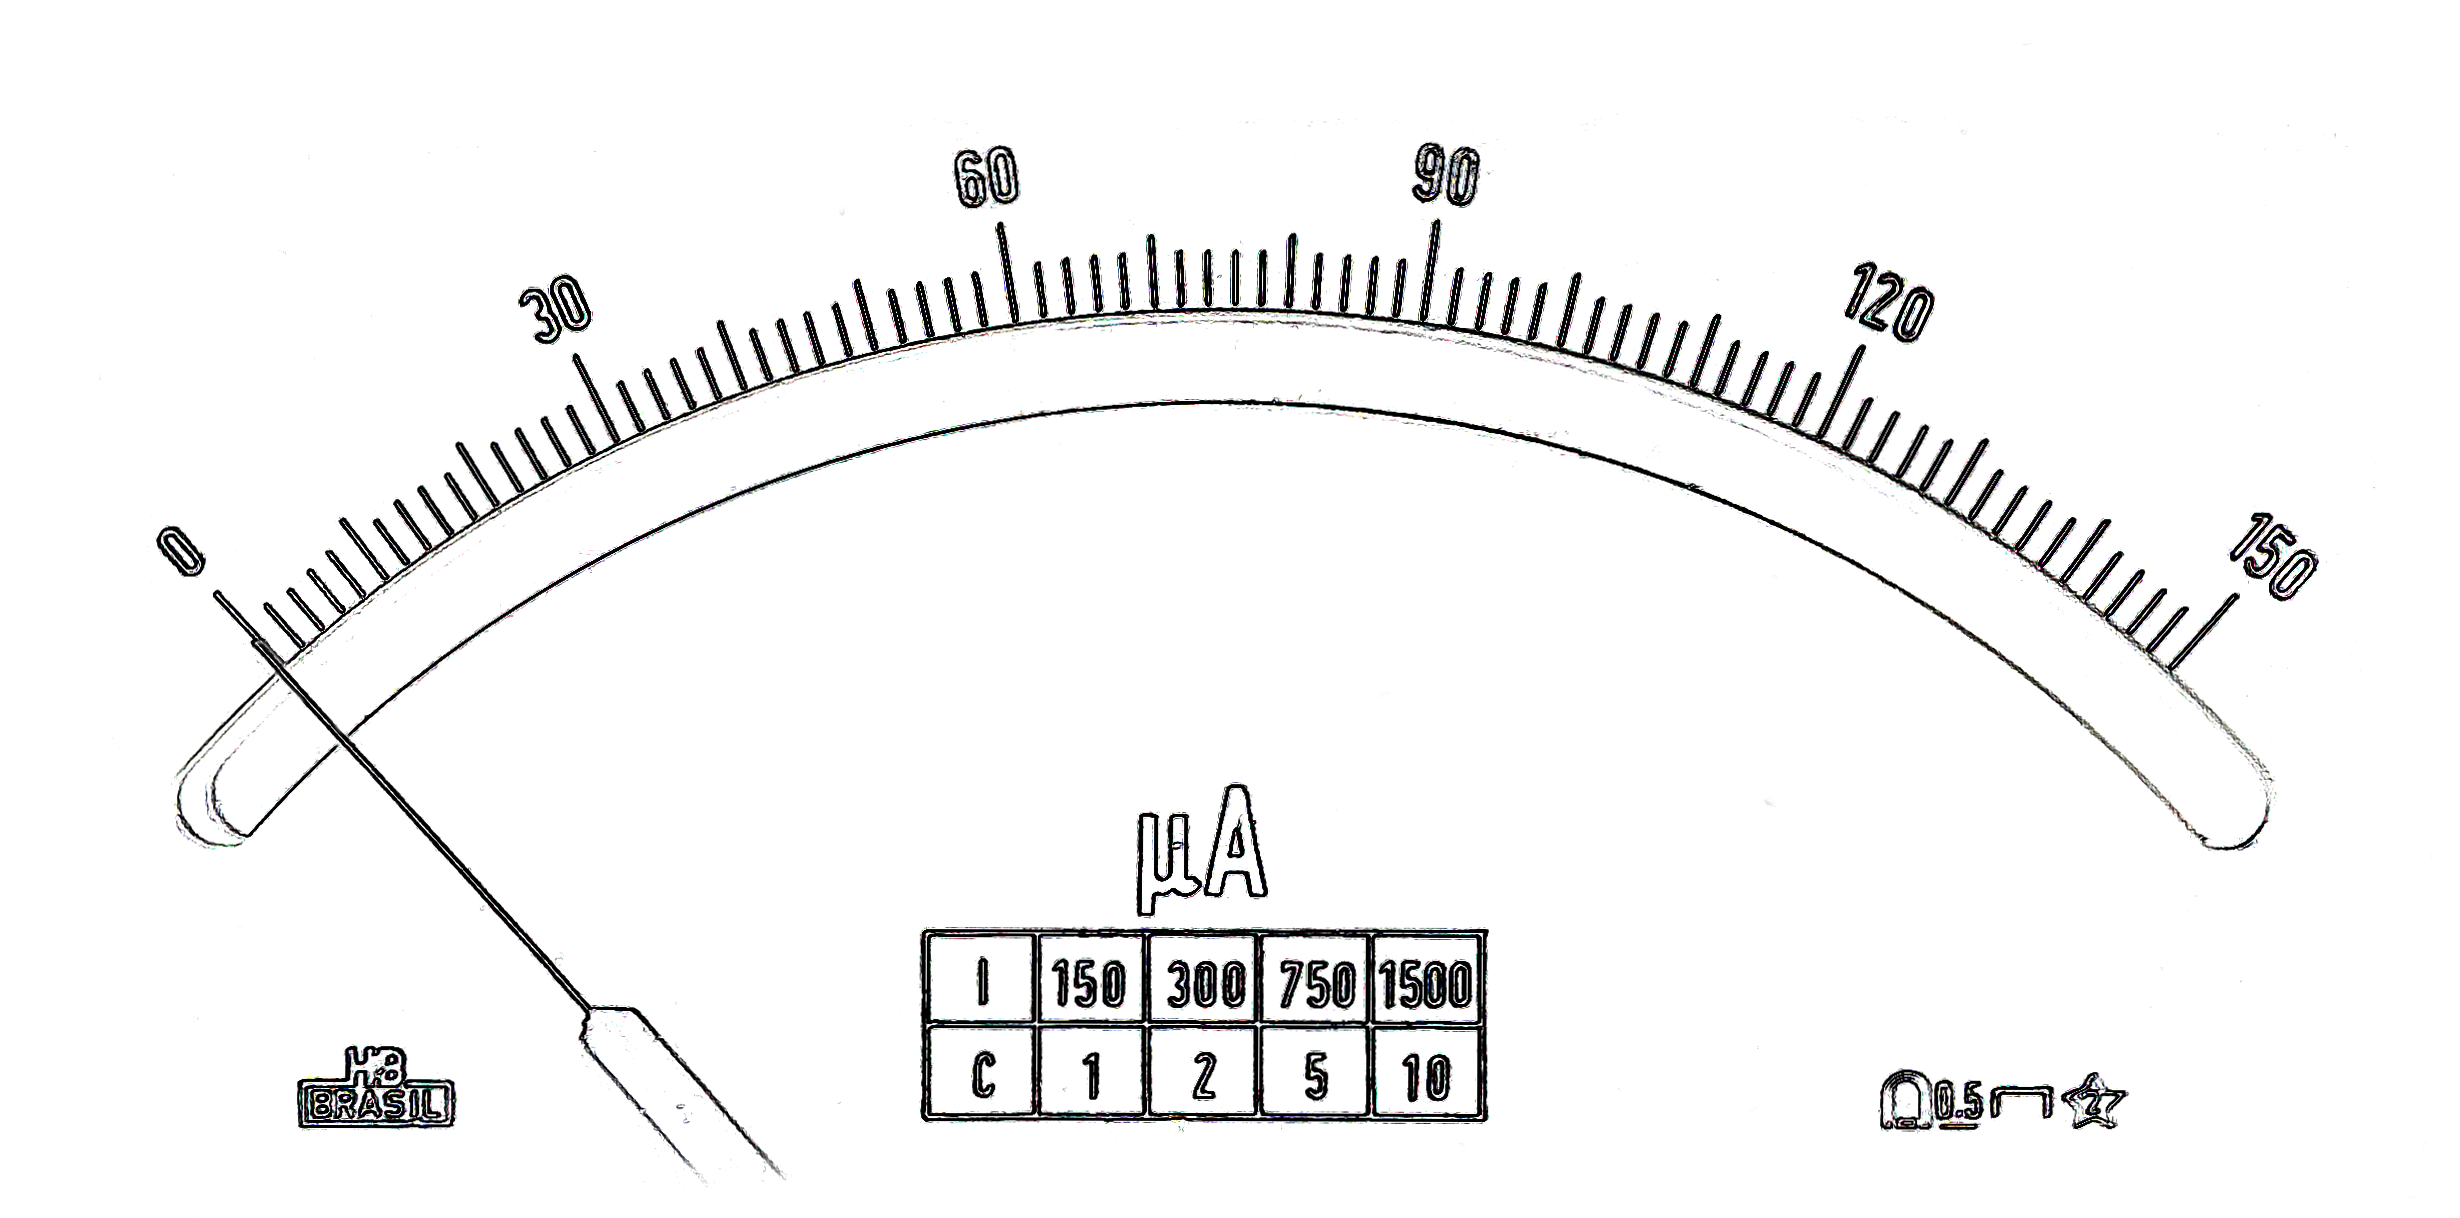
\includegraphics[width=\textwidth]{Ilustrations/AmperimetroAnalogEspelho.png}
	\caption{Para eliminar erros de leitura devidos à paralaxe, muitos equipamentos utilizam um espelho atrás do ponteiro (região curva abaixo da escala): quando a imagem do ponteiro no espelho está atrás do próprio ponteiro, temos certeza de que estamos vendo o ponteiro exatamente de frente, eliminando este tipo de erro.}
\end{marginfigure}

	Um erro pequeno pode ser cometido na própria leitura dos valores devido à paralaxe (deslocamento aparente entre dois objetos localizados a distâncias diferentes do observador quando este se move). Isso é bastante notável em equipamentos analógicos em que a medida é mostrada por um ponteiro, pois quando o observador se desloca uma pequena distância para um lado ou outro, a posição aparente do ponteiro muda. Para evitar o erro de paralaxe, a medida deve ser feita de forma que o ponteiro seja observado diretamente de frente. Alguns aparelhos têm uma região espelhada atrás do ponteiro para eliminar esse tipo de erro, sendo que a leitura correta é feita quando a imagem do ponteiro fica escondida atrás dele.
	
	Em alguns equipamentos, a menor divisão da escala\footnote{O valor da menor divisão da escala de um instrumento é conhecido como a sua \emph{resolução}.} pode ser muito grande. Nesse caso, temos mais facilidade em avaliar o algarismo estimado. Podemos então reduzir o valor do erro para \nicefrac{1}{3} ou \nicefrac{1}{4} da medida. No entanto isso não é muito comum, pois em geral os fabricantes dos equipamentos optam por divisões pequenas com o intuito de possibilitar a realização de medidas precisas. Nos equipamentos que utilizaremos no laboratório didático, as divisões são em geral pequenas e por isso adotaremos sempre que o erro é equivalente à metade da menor divisão da escala.

	\item[Equipamentos digitais ou dotados de escala auxiliar:] Se, por outro lado, o equipamento for digital podemos realizar uma medida como $M = \np[g]{14,2}$, por exemplo. Se utilizássemos um equipamento mais preciso, talvez essa medida pudesse variar entre \np[g]{14,15} até \np[g]{14,25} (incluindo o primeiro valor, porém não incluindo o último) devido a arredondamentos realizados pelo equipamento em virtude do número reduzido de casas decimais. Outra possibilidade é a de que o equipamento simplesmente descarte dígitos menores que décimos de grama, o que permitiria que as medidas variassem entre \np[g]{14,20} e \np[g]{14,29}. Poderíamos escolher para o erro do equipamento o valor de metade da menor divisão da escala abaixo do valor mostrado e de uma divisão acima. Por simplicidade, no entanto, \emph{assumimos que no caso de equipamentos digitais o erro é equivalente à menor divisão da escala tanto acima quanto abaixo do valor indicado}.
	
	Se o equipamento é dotado de uma escala auxiliar, verificamos que ao realizar a leitura em geral percebemos que duas ou três marcar parecem alinhadas com as marcas da escala principal. Se tormarmos a do meio, por exemplo, poderíamos considerar que a medida pode variar dentro do intervalo compreendido pelas marcas à esquerda e à direita. Logo, também adotamos para o erro a menor divisão da escala. Como tanto os equipamentos digitais, quanto os dotados de escala auxiliar possuem erros dados pela mesma regra, equipamentos desses dois tipos são comumente referidos coletivamente como \emph{não-analógicos}.
\end{description}

%%%%%%%%%%%%%%%%%%%%%%%%%%%
\section{Erros propagados}
%%%%%%%%%%%%%%%%%%%%%%%%%%%

Se precisamos calcular a área de uma folha, é mais fácil realizar um cálculo através do produto das medidas de ambos os lados, que comparar com um ``padrão de área''. Se temos um erro nas medidas das laterais, no entanto, deve haver um erro associado à medida da área.

Na Figura~\ref{Fig:ErroArea} mostramos o cálculo da área a partir de duas medidas $\ell_1$ e $\ell_2$. Como cada uma dessas medidas possui um erro associado, denotados por $\delta\ell_1$ e $\delta\ell_2$, respectivamente, devemos calcular os valores máximos e mínimos da área:
%
\begin{marginfigure}[2cm]
\centering
\begin{tikzpicture}[scale=1.5]
	\draw[thick] (0,0) rectangle (2,3);
	\draw[dashed,thin] (1.9,0) -- (1.9,2.9);
	\draw[dashed,thin] (2.1,0) -- (2.1,3.1);
	\draw[dashed,thin] (0,2.9) -- (1.9,2.9);
	\draw[dashed,thin] (0,3.1) -- (2.1,3.1);
	
	\draw[|-|] (-0.2,0) -- node[left]{$\ell_1$} (-0.2,3);
	
	\draw[|-|] (0, -0.2) -- node[below]{$\ell_2$} (2, -0.2);
\end{tikzpicture}
\caption{Erro no cálculo da área de um retângulo.}
\label{Fig:ErroArea}
\end{marginfigure}
%
\begin{align}
	A_{-} &= (\ell_1 - \delta\ell_1)(\ell_2 - \delta\ell_2) \\
	&= \ell_1\ell_2 - (\ell_1 \,\delta\ell_2 + \ell_2\,\delta\ell_1 - \delta\ell_1\,\delta\ell_2)
\end{align}

\begin{align}
	A_{+} &= (\ell_1 + \delta\ell_1)(\ell_2 + \delta\ell_2) \\
	&= \ell_1\ell_2 + (\ell_1 \,\delta\ell_2 + \ell_2\,\delta\ell_1 + \delta\ell_1\,\delta\ell_2).
\end{align}

\noindent{}Se desprezarmos o produto $\delta\ell_1\,\delta\ell_2$, que deve ser muito pequeno, já que os erros são -- em geral -- pequenas frações das medidas, temos
\begin{equation}
	A = \ell_1\ell_2 \pm (\ell_1\,\delta\ell_2+\ell_2\,\delta\ell_1).
\end{equation}
%
Temos então uma expressão para calcular o erro associado à área da folha. 

A expressão acima, não está limitada ao cálculo de uma área, mas serve para qualquer multiplicação de dois números. Veremos adiante que podemos calcular uma expressão geral para o cálculo do erro para qualquer expressão. A partir de tal expressão, podemos verificar os resultados abaixo
\begin{subequations}
\begin{align}
	(x\pm\delta x)+(y\pm\delta y) &= (x+y)\pm(\delta x+\delta y) \\
	(x\pm\delta x)-(y\pm\delta y) &= (x-y)\pm(\delta x + \delta y) \\
	(x\pm\delta x) \cdot (y\pm\delta y) &= (x\cdot y)\pm (|x|\cdot\delta y + |y|\cdot\delta x) \\
	(x\pm \delta x)\div(y\pm\delta y) &= (x\div y)\pm\frac{|x|\cdot\delta y+|y|\cdot\delta x}{y^2} \\
	(x\pm\delta x)^n &= x^n\pm n \cdot x^{n-1}\cdot\delta x \\
	\ln(x\pm\delta x) &= \ln x \pm \frac{\delta x}{x} \\
	\log (x\pm\delta x) &= \log x \pm \frac{0,4343\cdot\delta x}{x}.
\end{align}
\end{subequations}
%
É importante observar, no entanto, que apesar de podermos calcular o erro propagado em uma operação complexa como uma sucessão de operações simples --~como as do conjunto de equações acima~-- em geral esse erro é maior do que aquele que seria obtido se deduzíssemos a expressão para o erro a partir da expressão geral para o erro propagado.

%%%%%%%%%%%%%%%%%%%%%%%%%%%%%%%%%%%%%%%%%%
\subsection{Constantes e erros propagados}
%%%%%%%%%%%%%%%%%%%%%%%%%%%%%%%%%%%%%%%%%%

No caso de termos operações envolvendo constantes como $\pi$, ou qualquer outro valor conhecido absolutamente (como 2, 3, 4, etc.) --~isto é, que não são medidas~--, podemos simplesmente efetuar a operação com a constante e o erro da mesma forma que com a medida. Por exemplo
\begin{align}
     r &= (\numprint{4,0} \pm \numprint{0,5})\textrm{~mm} \\
     p &= 2\pi r \\
     &= 2\pi(\numprint{4,0} \pm \numprint{0,5})\textrm{~mm} \\
     &= (2\pi\,\numprint{4,0} \pm 2\pi\,\numprint{0,5})\textrm{~mm} \\
     &= (25 \pm 3)~\textrm{~mm}
\end{align}
%
sempre respeitando o número de algarismos significativos e os critérios de arredondamento.

%%%%%%%%%%%%%%%%%%%%%%%%%%%%%%%%%%%%%%%%%%%%%%
\section{Erros e algarismos significativos}
%%%%%%%%%%%%%%%%%%%%%%%%%%%%%%%%%%%%%%%%%%%%%%

Verificamos que as medidas fornecidas por instrumentos são expressas por um conjunto de algarismos significativos e que algarismos além deles eram mera especulação. Também utilizamos regras gerais para determinar o número de algarismos significativos de uma medida indireta com base no número de algarismos significativos das medidas diretas. Agora que conhecemos o erro, podemos entender a origem dos algarismos significativos de uma maneira simples: eles são os algarismos cuja ordem de grandeza é maior ou igual àquela do erro. %\comment{Existem casos em que o erro propagado pode ser maior ou menor que o último significativo, o que fazer nesse caso?}

Para verificar como funciona esse processo, vejamos o seguinte conjunto de medidas:
\begin{align}
	v_0 &= (\numprint{10,3456} \pm \numprint{0,01})~\textrm{m}/\textrm{s} \label{medidas_v_start}\\
	a &= (\numprint{2,0658} \pm \numprint{0,05})~\textrm{m}/\textrm{s}^2 \\
	t &= (\numprint{3,000} \pm \numprint{0,001})~\textrm{s} \label{medidas_v_end}.
\end{align}
%
Utilizando essas informações e as fórmulas para o erro propagado, obtemos -- utilizando a relação $v = v_0 + at$ -- o seguinte resultado:
\begin{equation}
	v = (\numprint{16,543} \pm \numprint{0,1620658})~\textrm{m}/\textrm{s}.
\end{equation}
%
O erro é sempre expresso com um ou dois algarismos significativos\footnote{Lembre-se que utilizamos dois se o primeiro algarismo significativo do erro, isto é, o primeiro dígito diferente de zero, for 1; nos demais casos utilizamos somente um algarismo significativo.}. Nesse caso, o erro da medida acima pode ser expresso como $\delta v = \np[m/s]{0,16}$. A medida acima tem algarismos cuja ordem de grandeza é menor que o erro e são, portanto, sem significado. Podemos reduzir nossa medida para a velocidade a
\begin{equation}\label{ResultadoAlgSigErro}
	v = (\numprint{16,54} \pm \numprint{0,16})~\textrm{m}/\textrm{s}.
\end{equation}

Analisando o erro das medidas mostradas nas Equações~\eqref{medidas_v_start} a~\eqref{medidas_v_end}, percebemos que existem vários algarismos sem significado. Retirando-os, obtemos
\begin{align}
	v_0 &= (\numprint{10,35} \pm \numprint{0,01})~\textrm{m}/\textrm{s} \\
	a &= (\numprint{2,07} \pm \numprint{0,05})~\textrm{m}/\textrm{s}^2 \\
	t &= (\numprint{3,000} \pm \numprint{0,001})~\textrm{s}.
\end{align}
%
Verificamos agora que a medida para a aceleração $a$ tem somente três algarismos significativos. Segundo a regra sobre o número de algarismos significativos para o resuldado de uma multiplicação, devemos manter então somente três algarismos. Ao somarmos com o valor de $v_0$, a regra nos diz para mantermos duas casas após a vírgula. De fato, isto nos dá um resultado que coincide com aquele obtido através da análise do erro propagado (Equação~\eqref{ResultadoAlgSigErro}).

%\comment{Em alguns casos o erro fica menor do que o último algarismo duvidoso (pelo menos observei isso em alguns cálculos hipotéticos). E aí? Existem casos em que o erro fique maior, forçando a descartar algarismos?}

%%%%%%%%%%%%%%%%%%%%%%%%%%%%%%%%%%%%%%%%%%%%%
\section{Incerteza fracional e percentual}
%%%%%%%%%%%%%%%%%%%%%%%%%%%%%%%%%%%%%%%%%%%%%

Se realizamos uma medição com um instrumento e obtemos $\ell_1 = (\numprint{15,3} \pm \numprint{0,5})~\textrm{cm}$, o erro é de aproximadamente \numprint{3,3}\%. Se realizarmos outra medição com o mesmo instrumento e obtivermos $\ell_2 = (\numprint{3,4} \pm \numprint{0,5})~\textrm{cm}$, teremos um erro de aproximadamente \numprint{14,7}\%. Claramente no segundo caso temos uma medida mais incerta que no primeiro, o que acarretará em consequências para o cálculo de medidas indiretas.

Para calcularmos o erro como uma fração da medida, basta o dividirmos pelo valor da medida:
\begin{equation}
	E_f = \frac{\delta x}{x}.
\end{equation}
%
Como $x$ e $\delta x$ possuem a mesma unidade, o erro fracional é adimensional. O erro percentual pode ser calculado multiplicando-se o erro fracional por 100:
\begin{equation}
	E_\% = 100 \cdot E_f.
\end{equation}

É comum encontrar dispositivos eletrônicos cujo erro é dado como um número percentual. Por exemplo, podemos ter um resistor cuja resistência $R$ é de $500~\Omega$, com erro de $5~\%$. Isso significa que a medida da resistência é $R = (500 \pm 25)~\Omega$, ou melhor, $R = (50 \pm 3)\times10^1~\Omega$. 

Outro uso comum do erro percentual é ao se declarar a precisão de um instrumento de medida. Se um voltímetro declara sua precisão como $1~\%$, isso significa que em uma medida $V_1 = \numprint{13,45}~\textrm{V}$ temos um erro  $\delta V_1 = \numprint{0,13}~\textrm{V}$. Já em uma medida $V_2 = \numprint{156,35}~\textrm{V}$, temos um erro $\delta V_2 = \numprint{1,6}~\textrm{V}$. Temos, portanto, um caso em que o erro da medida -- também chamado de \emph{erro absoluto} -- varia, mas o erro percentual é constante, indicando que o instrumento é igualmente adequado (ou inadequado, dependendo de sua necessidade de precisão) para uma ampla faixa de valores de medida.

Os erros fracional e percentual nos indicam que sempre que desejarmos conhecer uma medida calculada a partir de outras, devemos procurar utilizar medidas diretas com um grande número de algarismos significativos, de forma a minimizar o erro percentual. Por exemplo, se calcularmos o valor da aceleração da gravidade através de
\begin{equation}
	g = \frac{2\Delta x}{t^2},
\end{equation}
%
a partir das medidas 
\begin{align}
	t_1 &= (\numprint{0,15} \pm \numprint{0,01})~\textrm{s} \\
	\Delta x_1 &= (\numprint{0,11} \pm \numprint{0,02})~\textrm{m}
\end{align}
%
e
\begin{align}
	t_2 &= (\numprint{1,32} \pm \numprint{0,01})~\textrm{s} \\
	\Delta x_2 &= (\numprint{8,54} \pm \numprint{0,02})~\textrm{m},
\end{align}
%
obteremos os valores
\begin{align}
	g_1 &= (\numprint{9,8} \pm 2)~\textrm{m}/\textrm{s}^2 \\
	g_2 &= (\numprint{9,80} \pm \numprint{0,1})~\textrm{m}/\textrm{s}^2.
\end{align}
%
Claramente as medidas diretas têm o mesmo erro absoluto, no entanto erros fracionais/percentuais diferentes. Isso se reflete na incerteza da medida indireta, onde no segundo caso obtemos um erro muito menor, devido ao menor erro fracional/percentual.

%%%%%%%%%%%%%%%%%%%%%%%%%%%%%%%%%%%%%%%%%%%%%%%%%%%%%%%%%%%%%
\section{Expressão geral para o cálculo do erro propagado}
%%%%%%%%%%%%%%%%%%%%%%%%%%%%%%%%%%%%%%%%%%%%%%%%%%%%%%%%%%%%%
%\comment{Ver aqui se tem algum problema, tinha uns errinhos e tinha que substituir uns $d$ por $\delta$.}
Apesar de termos conseguido calcular o erro propagado de uma maneira relativamente simples para o caso do produto de duas medidas, precisamos de um método mais robusto, que possa sem aplicado a qualquer tipo de \emph{função}. Se tivermos uma medida $q$, dada por $q=f(x,y,z,\dots,\xi,\dots)$, onde $x$, $y$, $z$, \dots,$\xi$, \dots representam medidas diretas através das quais calculamos a medida indireta $q$. Podemos calcular uma variação em $q$ em relação a uma variação em uma das medidas, por exemplo na medida $\xi$, através de uma derivada, pois se temos
\begin{equation}
	\frac{dq}{d\xi} = \frac{df(x,y,z,\dots,\xi,\dots)}{d\xi},
\end{equation}
%
podemos escrever para a variação $dq$ através de 
\begin{equation}
	dq = \left(\frac{df(x,y,z,\dots,\xi,\dots)}{d\xi}\right)d\xi.
\end{equation}
%
Calculando a derivada total, temos
\begin{equation}
	\frac{dq}{d\xi} = \left(\frac{\partial f}{\partial x}\right) \frac{dx}{d\xi} + \left(\frac{\partial f}{\partial y}\right)\frac{dy}{d\xi} + \left(\frac{\partial f}{\partial z}\right) \frac{dz}{d\xi} + \dots + \left(\frac{\partial f}{\partial \xi}\right) \frac{d\xi}{d\xi} + \dots.
\end{equation}
%
Utilizamos aqui uma derivada total, ou diferencial exata, pois quando calculamos a derivada parcial em relação a um parâmetro, mantemos os demais constantes. No entanto, se qualquer dos parâmetros também depender daquele que está sendo variado, precisamos levar isso em conta. O primeiro termo a direita na equação acima, por exemplo, leva em conta a variação de $f$ em relação a $x$ e a variação deste em relação a $\xi$, enquanto o termo entre as reticências é o que leva em conta a variação direta de $f$ em relação a $\xi$. Verificamos então que a variação de $q$ pode ser escrita como
\begin{equation}
	dq = \left(\frac{\partial f}{\partial x}\right) dx + \left(\frac{\partial f}{\partial y}\right) dy + \left(\frac{\partial f}{\partial z}\right) dz + \dots + \left(\frac{\partial f}{\partial \xi}\right) d\xi + \dots.
\end{equation}

As variações nas medidas mencionadas acima podem ser consideradas como sendo os próprios erros de medida. Nesse caso, podemos afirmar que a equação acima nos dá o \emph{erro propagado}. Como pode haver um cancelamento dos erros com a expressão acima no caso de algumas variações serem positivas e outras serem negativas, podemos tomar o módulo de cada termo para encontrar o erro máximo:
\begin{equation}\label{Eq:ErroGeral}
	\delta q = \left|\frac{\partial f}{\partial x}\right| dx + \left|\frac{\partial f}{\partial y}\right| dy + \left|\frac{\partial f}{\partial z}\right| dz + \dots + \left|\frac{\partial f}{\partial \xi}\right| d\xi + \dots.
\end{equation}

A partir da equação acima, podemos calcular o erro para qualquer função que nos dê uma medida indireta. Se considerarmos que a área de um retângulo é dado por $A=f(\ell_1,\ell_2)=\ell_1\ell_2$, temos:
\begin{align}
	\delta A &= \left|\frac{\partial(\ell_1\ell_2)}{\partial \ell_1}\right|\delta \ell_1 + \left|\frac{\partial (\ell_1\ell_2)}{\partial \ell_2}\right|\delta y \\
	&= |\ell_2|\delta \ell_1 + |\ell_1|\delta 2,
\end{align}
%
que é exatamente a expressão que encontramos quando analisamos os valores máximo e mínimo para a área do retângulo. 

%%%%%%%%%%%%%%%%%%%%%%%%%%%%%%%%%%%%%%%%%
%\section{Representando erros em gráficos}
%%%%%%%%%%%%%%%%%%%%%%%%%%%%%%%%%%%%%%%%%

%\comment{Falar e dar exemplos de barras de erro (simétricas, assimétricas)}




\chapter{Regressão Linear}
\label{Chap:RegressoLinear}

\begin{fullwidth}
{\it
Apesar de podermos verificar previsões teóricas pela simples comparação com os dados experimentais obtidos (assumindo que eles sejam confiáveis), devido à dispersão dos dados não temos um bom método para extrair informações a partir das medidas. Veremos que para isso precisamos determinar a linha de tendência dos dados. A partir das informações para essa linha, conseguiremos extrair informações acerca de parâmetros físicos do sistema.
}
\end{fullwidth}

%%%%%%%%%%%%%%%%%%%%%%%%%%%%%%%%%%%%%
\section{Linhas de Tendência}
%%%%%%%%%%%%%%%%%%%%%%%%%%%%%%%%%%%%%

Quando realizamos um experimento, procuramos relacionar uma variável dependente a uma variável independente. Para visualizarmos a relação entre as duas, é interessante fazer uma representação gráfica da variável dependente em função dos valores da variável independente. Podemos assim verificar uma tendência geral dos pontos, que pode seguir padrões retilíneos, parabólicos, etc. Retomando a citação ao texto de Johann H. Lambert (e a extendendo), temos\cite{Lambert}
\begin{quote}
Se as observações experimentais fossem completamente precisas, essas ordenadas resultariam em um número de pontos através dos quais uma curva ou uma reta deveriam ser traçadas. No entanto, esse não é o caso, a curva/reta desvia pouco ou muito dos pontos observados. Portanto, ela deve ser traçada de maneira que passe tão próxima quanto possível das posições verdadeiras e vá, como se fosse, pelo meio dos pontos em questão.
\end{quote}
%
Muitas vezes tal padrão é muito claro, pois os pontos tem uma \emph{dispersão} baixa. Outras vezes a dispersão é razoavelmente alta e fica difícil verificar o padrão seguido pelos pontos.

Mesmo em casos em que podemos verificar um padrão aparente ao fazer um gráfico, determinar a forma mais adequada para a \emph{linha de tendência} que melhor descreve os pontos experimentais ---~ou mesmo afirmar que tais pontos seguem este padrão~--- pode ser complicado. Se, por exemplo, fizermos uma série de medidas que seguem um padrão parabólico, mas com medidas que se restringem a um intervalo pequeno da variável independente, o gráfico terá a aparência de uma reta (veja as Figuras~\ref{Fig:ParabolaReta} e~\ref{Fig:ParabolaReta2}).
\begin{figure*}
\centering
\forceversofloat
\caption{Gráfico de um conjunto de pontos que aparentemente seguem uma tendência linear. Veja também a Figura~\ref{Fig:ParabolaReta2}.}
\label{Fig:ParabolaReta}
\begin{tikzpicture}[gnuplot]
%% generated with GNUPLOT 5.0p6 (Lua 5.3; terminal rev. 99, script rev. 100)
%% seg 30 jul 2018 13:30:47 -03
\path (0.000,0.000) rectangle (14.000,9.000);
\gpcolor{color=gp lt color border}
\gpsetlinetype{gp lt border}
\gpsetdashtype{gp dt solid}
\gpsetlinewidth{1.00}
\draw[gp path] (1.136,0.985)--(1.316,0.985);
\draw[gp path] (13.447,0.985)--(13.267,0.985);
\node[gp node right] at (0.952,0.985) {$15$};
\draw[gp path] (1.136,2.259)--(1.316,2.259);
\draw[gp path] (13.447,2.259)--(13.267,2.259);
\node[gp node right] at (0.952,2.259) {$20$};
\draw[gp path] (1.136,3.534)--(1.316,3.534);
\draw[gp path] (13.447,3.534)--(13.267,3.534);
\node[gp node right] at (0.952,3.534) {$25$};
\draw[gp path] (1.136,4.808)--(1.316,4.808);
\draw[gp path] (13.447,4.808)--(13.267,4.808);
\node[gp node right] at (0.952,4.808) {$30$};
\draw[gp path] (1.136,6.082)--(1.316,6.082);
\draw[gp path] (13.447,6.082)--(13.267,6.082);
\node[gp node right] at (0.952,6.082) {$35$};
\draw[gp path] (1.136,7.357)--(1.316,7.357);
\draw[gp path] (13.447,7.357)--(13.267,7.357);
\node[gp node right] at (0.952,7.357) {$40$};
\draw[gp path] (1.136,8.631)--(1.316,8.631);
\draw[gp path] (13.447,8.631)--(13.267,8.631);
\node[gp node right] at (0.952,8.631) {$45$};
\draw[gp path] (1.460,0.985)--(1.460,1.165);
\draw[gp path] (1.460,8.631)--(1.460,8.451);
\node[gp node center] at (1.460,0.677) {$3.8$};
\draw[gp path] (2.756,0.985)--(2.756,1.165);
\draw[gp path] (2.756,8.631)--(2.756,8.451);
\node[gp node center] at (2.756,0.677) {$4$};
\draw[gp path] (4.052,0.985)--(4.052,1.165);
\draw[gp path] (4.052,8.631)--(4.052,8.451);
\node[gp node center] at (4.052,0.677) {$4.2$};
\draw[gp path] (5.348,0.985)--(5.348,1.165);
\draw[gp path] (5.348,8.631)--(5.348,8.451);
\node[gp node center] at (5.348,0.677) {$4.4$};
\draw[gp path] (6.644,0.985)--(6.644,1.165);
\draw[gp path] (6.644,8.631)--(6.644,8.451);
\node[gp node center] at (6.644,0.677) {$4.6$};
\draw[gp path] (7.939,0.985)--(7.939,1.165);
\draw[gp path] (7.939,8.631)--(7.939,8.451);
\node[gp node center] at (7.939,0.677) {$4.8$};
\draw[gp path] (9.235,0.985)--(9.235,1.165);
\draw[gp path] (9.235,8.631)--(9.235,8.451);
\node[gp node center] at (9.235,0.677) {$5$};
\draw[gp path] (10.531,0.985)--(10.531,1.165);
\draw[gp path] (10.531,8.631)--(10.531,8.451);
\node[gp node center] at (10.531,0.677) {$5.2$};
\draw[gp path] (11.827,0.985)--(11.827,1.165);
\draw[gp path] (11.827,8.631)--(11.827,8.451);
\node[gp node center] at (11.827,0.677) {$5.4$};
\draw[gp path] (13.123,0.985)--(13.123,1.165);
\draw[gp path] (13.123,8.631)--(13.123,8.451);
\node[gp node center] at (13.123,0.677) {$5.6$};
\draw[gp path] (1.136,8.631)--(1.136,0.985)--(13.447,0.985)--(13.447,8.631)--cycle;
\node[gp node center,rotate=-270] at (0.246,4.808) {$y$};
\node[gp node center] at (7.291,0.215) {$x$};
\node[gp node left] at (2.604,8.297) {Dados experimentais};
\gpcolor{rgb color={0.000,0.000,0.000}}
\gpsetpointsize{4.00}
\gppoint{gp mark 7}{(2.108,1.395)}
\gppoint{gp mark 7}{(3.404,3.299)}
\gppoint{gp mark 7}{(4.700,3.465)}
\gppoint{gp mark 7}{(5.996,2.400)}
\gppoint{gp mark 7}{(7.292,4.362)}
\gppoint{gp mark 7}{(8.587,5.265)}
\gppoint{gp mark 7}{(9.883,5.916)}
\gppoint{gp mark 7}{(11.179,6.895)}
\gppoint{gp mark 7}{(12.475,7.645)}
\gppoint{gp mark 7}{(1.962,8.297)}
\gpcolor{color=gp lt color border}
\node[gp node left] at (2.604,7.989) {$y = \np{14.24113} \, x - \np{38.07973}$, $r^2 = \np{0.90858}$};
\gpcolor{rgb color={0.000,0.000,0.000}}
\draw[gp path] (1.504,7.989)--(2.420,7.989);
\draw[gp path] (1.788,1.433)--(1.795,1.437)--(1.801,1.440)--(1.807,1.444)--(1.813,1.447)%
  --(1.819,1.450)--(1.825,1.454)--(1.832,1.457)--(1.838,1.461)--(1.844,1.464)--(1.850,1.468)%
  --(1.856,1.471)--(1.862,1.475)--(1.869,1.478)--(1.875,1.481)--(1.881,1.485)--(1.887,1.488)%
  --(1.893,1.492)--(1.899,1.495)--(1.905,1.499)--(1.912,1.502)--(1.918,1.506)--(1.924,1.509)%
  --(1.930,1.513)--(1.936,1.516)--(1.942,1.519)--(1.949,1.523)--(1.955,1.526)--(1.961,1.530)%
  --(1.967,1.533)--(1.973,1.537)--(1.979,1.540)--(1.985,1.544)--(1.992,1.547)--(1.998,1.550)%
  --(2.004,1.554)--(2.010,1.557)--(2.016,1.561)--(2.022,1.564)--(2.029,1.568)--(2.035,1.571)%
  --(2.041,1.575)--(2.047,1.578)--(2.053,1.581)--(2.059,1.585)--(2.065,1.588)--(2.072,1.592)%
  --(2.078,1.595)--(2.084,1.599)--(2.090,1.602)--(2.096,1.606)--(2.102,1.609)--(2.109,1.613)%
  --(2.115,1.616)--(2.121,1.619)--(2.127,1.623)--(2.133,1.626)--(2.139,1.630)--(2.146,1.633)%
  --(2.152,1.637)--(2.158,1.640)--(2.164,1.644)--(2.170,1.647)--(2.176,1.650)--(2.182,1.654)%
  --(2.189,1.657)--(2.195,1.661)--(2.201,1.664)--(2.207,1.668)--(2.213,1.671)--(2.219,1.675)%
  --(2.226,1.678)--(2.232,1.681)--(2.238,1.685)--(2.244,1.688)--(2.250,1.692)--(2.256,1.695)%
  --(2.262,1.699)--(2.269,1.702)--(2.275,1.706)--(2.281,1.709)--(2.287,1.713)--(2.293,1.716)%
  --(2.299,1.719)--(2.306,1.723)--(2.312,1.726)--(2.318,1.730)--(2.324,1.733)--(2.330,1.737)%
  --(2.336,1.740)--(2.342,1.744)--(2.349,1.747)--(2.355,1.750)--(2.361,1.754)--(2.367,1.757)%
  --(2.373,1.761)--(2.379,1.764)--(2.386,1.768)--(2.392,1.771)--(2.398,1.775)--(2.404,1.778)%
  --(2.410,1.781)--(2.416,1.785)--(2.422,1.788)--(2.429,1.792)--(2.435,1.795)--(2.441,1.799)%
  --(2.447,1.802)--(2.453,1.806)--(2.459,1.809)--(2.466,1.813)--(2.472,1.816)--(2.478,1.819)%
  --(2.484,1.823)--(2.490,1.826)--(2.496,1.830)--(2.503,1.833)--(2.509,1.837)--(2.515,1.840)%
  --(2.521,1.844)--(2.527,1.847)--(2.533,1.850)--(2.539,1.854)--(2.546,1.857)--(2.552,1.861)%
  --(2.558,1.864)--(2.564,1.868)--(2.570,1.871)--(2.576,1.875)--(2.583,1.878)--(2.589,1.881)%
  --(2.595,1.885)--(2.601,1.888)--(2.607,1.892)--(2.613,1.895)--(2.619,1.899)--(2.626,1.902)%
  --(2.632,1.906)--(2.638,1.909)--(2.644,1.912)--(2.650,1.916)--(2.656,1.919)--(2.663,1.923)%
  --(2.669,1.926)--(2.675,1.930)--(2.681,1.933)--(2.687,1.937)--(2.693,1.940)--(2.699,1.944)%
  --(2.706,1.947)--(2.712,1.950)--(2.718,1.954)--(2.724,1.957)--(2.730,1.961)--(2.736,1.964)%
  --(2.743,1.968)--(2.749,1.971)--(2.755,1.975)--(2.761,1.978)--(2.767,1.981)--(2.773,1.985)%
  --(2.780,1.988)--(2.786,1.992)--(2.792,1.995)--(2.798,1.999)--(2.804,2.002)--(2.810,2.006)%
  --(2.816,2.009)--(2.823,2.012)--(2.829,2.016)--(2.835,2.019)--(2.841,2.023)--(2.847,2.026)%
  --(2.853,2.030)--(2.860,2.033)--(2.866,2.037)--(2.872,2.040)--(2.878,2.044)--(2.884,2.047)%
  --(2.890,2.050)--(2.896,2.054)--(2.903,2.057)--(2.909,2.061)--(2.915,2.064)--(2.921,2.068)%
  --(2.927,2.071)--(2.933,2.075)--(2.940,2.078)--(2.946,2.081)--(2.952,2.085)--(2.958,2.088)%
  --(2.964,2.092)--(2.970,2.095)--(2.976,2.099)--(2.983,2.102)--(2.989,2.106)--(2.995,2.109)%
  --(3.001,2.112)--(3.007,2.116)--(3.013,2.119)--(3.020,2.123)--(3.026,2.126)--(3.032,2.130)%
  --(3.038,2.133)--(3.044,2.137)--(3.050,2.140)--(3.057,2.144)--(3.063,2.147)--(3.069,2.150)%
  --(3.075,2.154)--(3.081,2.157)--(3.087,2.161)--(3.093,2.164)--(3.100,2.168)--(3.106,2.171)%
  --(3.112,2.175)--(3.118,2.178)--(3.124,2.181)--(3.130,2.185)--(3.137,2.188)--(3.143,2.192)%
  --(3.149,2.195)--(3.155,2.199)--(3.161,2.202)--(3.167,2.206)--(3.173,2.209)--(3.180,2.212)%
  --(3.186,2.216)--(3.192,2.219)--(3.198,2.223)--(3.204,2.226)--(3.210,2.230)--(3.217,2.233)%
  --(3.223,2.237)--(3.229,2.240)--(3.235,2.244)--(3.241,2.247)--(3.247,2.250)--(3.253,2.254)%
  --(3.260,2.257)--(3.266,2.261)--(3.272,2.264)--(3.278,2.268)--(3.284,2.271)--(3.290,2.275)%
  --(3.297,2.278)--(3.303,2.281)--(3.309,2.285)--(3.315,2.288)--(3.321,2.292)--(3.327,2.295)%
  --(3.334,2.299)--(3.340,2.302)--(3.346,2.306)--(3.352,2.309)--(3.358,2.312)--(3.364,2.316)%
  --(3.370,2.319)--(3.377,2.323)--(3.383,2.326)--(3.389,2.330)--(3.395,2.333)--(3.401,2.337)%
  --(3.407,2.340)--(3.414,2.344)--(3.420,2.347)--(3.426,2.350)--(3.432,2.354)--(3.438,2.357)%
  --(3.444,2.361)--(3.450,2.364)--(3.457,2.368)--(3.463,2.371)--(3.469,2.375)--(3.475,2.378)%
  --(3.481,2.381)--(3.487,2.385)--(3.494,2.388)--(3.500,2.392)--(3.506,2.395)--(3.512,2.399)%
  --(3.518,2.402)--(3.524,2.406)--(3.530,2.409)--(3.537,2.412)--(3.543,2.416)--(3.549,2.419)%
  --(3.555,2.423)--(3.561,2.426)--(3.567,2.430)--(3.574,2.433)--(3.580,2.437)--(3.586,2.440)%
  --(3.592,2.444)--(3.598,2.447)--(3.604,2.450)--(3.611,2.454)--(3.617,2.457)--(3.623,2.461)%
  --(3.629,2.464)--(3.635,2.468)--(3.641,2.471)--(3.647,2.475)--(3.654,2.478)--(3.660,2.481)%
  --(3.666,2.485)--(3.672,2.488)--(3.678,2.492)--(3.684,2.495)--(3.691,2.499)--(3.697,2.502)%
  --(3.703,2.506)--(3.709,2.509)--(3.715,2.512)--(3.721,2.516)--(3.727,2.519)--(3.734,2.523)%
  --(3.740,2.526)--(3.746,2.530)--(3.752,2.533)--(3.758,2.537)--(3.764,2.540)--(3.771,2.544)%
  --(3.777,2.547)--(3.783,2.550)--(3.789,2.554)--(3.795,2.557)--(3.801,2.561)--(3.807,2.564)%
  --(3.814,2.568)--(3.820,2.571)--(3.826,2.575)--(3.832,2.578)--(3.838,2.581)--(3.844,2.585)%
  --(3.851,2.588)--(3.857,2.592)--(3.863,2.595)--(3.869,2.599)--(3.875,2.602)--(3.881,2.606)%
  --(3.888,2.609)--(3.894,2.612)--(3.900,2.616)--(3.906,2.619)--(3.912,2.623)--(3.918,2.626)%
  --(3.924,2.630)--(3.931,2.633)--(3.937,2.637)--(3.943,2.640)--(3.949,2.643)--(3.955,2.647)%
  --(3.961,2.650)--(3.968,2.654)--(3.974,2.657)--(3.980,2.661)--(3.986,2.664)--(3.992,2.668)%
  --(3.998,2.671)--(4.004,2.675)--(4.011,2.678)--(4.017,2.681)--(4.023,2.685)--(4.029,2.688)%
  --(4.035,2.692)--(4.041,2.695)--(4.048,2.699)--(4.054,2.702)--(4.060,2.706)--(4.066,2.709)%
  --(4.072,2.712)--(4.078,2.716)--(4.084,2.719)--(4.091,2.723)--(4.097,2.726)--(4.103,2.730)%
  --(4.109,2.733)--(4.115,2.737)--(4.121,2.740)--(4.128,2.743)--(4.134,2.747)--(4.140,2.750)%
  --(4.146,2.754)--(4.152,2.757)--(4.158,2.761)--(4.165,2.764)--(4.171,2.768)--(4.177,2.771)%
  --(4.183,2.775)--(4.189,2.778)--(4.195,2.781)--(4.201,2.785)--(4.208,2.788)--(4.214,2.792)%
  --(4.220,2.795)--(4.226,2.799)--(4.232,2.802)--(4.238,2.806)--(4.245,2.809)--(4.251,2.812)%
  --(4.257,2.816)--(4.263,2.819)--(4.269,2.823)--(4.275,2.826)--(4.281,2.830)--(4.288,2.833)%
  --(4.294,2.837)--(4.300,2.840)--(4.306,2.843)--(4.312,2.847)--(4.318,2.850)--(4.325,2.854)%
  --(4.331,2.857)--(4.337,2.861)--(4.343,2.864)--(4.349,2.868)--(4.355,2.871)--(4.361,2.875)%
  --(4.368,2.878)--(4.374,2.881)--(4.380,2.885)--(4.386,2.888)--(4.392,2.892)--(4.398,2.895)%
  --(4.405,2.899)--(4.411,2.902)--(4.417,2.906)--(4.423,2.909)--(4.429,2.912)--(4.435,2.916)%
  --(4.442,2.919)--(4.448,2.923)--(4.454,2.926)--(4.460,2.930)--(4.466,2.933)--(4.472,2.937)%
  --(4.478,2.940)--(4.485,2.943)--(4.491,2.947)--(4.497,2.950)--(4.503,2.954)--(4.509,2.957)%
  --(4.515,2.961)--(4.522,2.964)--(4.528,2.968)--(4.534,2.971)--(4.540,2.975)--(4.546,2.978)%
  --(4.552,2.981)--(4.558,2.985)--(4.565,2.988)--(4.571,2.992)--(4.577,2.995)--(4.583,2.999)%
  --(4.589,3.002)--(4.595,3.006)--(4.602,3.009)--(4.608,3.012)--(4.614,3.016)--(4.620,3.019)%
  --(4.626,3.023)--(4.632,3.026)--(4.638,3.030)--(4.645,3.033)--(4.651,3.037)--(4.657,3.040)%
  --(4.663,3.043)--(4.669,3.047)--(4.675,3.050)--(4.682,3.054)--(4.688,3.057)--(4.694,3.061)%
  --(4.700,3.064)--(4.706,3.068)--(4.712,3.071)--(4.719,3.075)--(4.725,3.078)--(4.731,3.081)%
  --(4.737,3.085)--(4.743,3.088)--(4.749,3.092)--(4.755,3.095)--(4.762,3.099)--(4.768,3.102)%
  --(4.774,3.106)--(4.780,3.109)--(4.786,3.112)--(4.792,3.116)--(4.799,3.119)--(4.805,3.123)%
  --(4.811,3.126)--(4.817,3.130)--(4.823,3.133)--(4.829,3.137)--(4.835,3.140)--(4.842,3.143)%
  --(4.848,3.147)--(4.854,3.150)--(4.860,3.154)--(4.866,3.157)--(4.872,3.161)--(4.879,3.164)%
  --(4.885,3.168)--(4.891,3.171)--(4.897,3.175)--(4.903,3.178)--(4.909,3.181)--(4.915,3.185)%
  --(4.922,3.188)--(4.928,3.192)--(4.934,3.195)--(4.940,3.199)--(4.946,3.202)--(4.952,3.206)%
  --(4.959,3.209)--(4.965,3.212)--(4.971,3.216)--(4.977,3.219)--(4.983,3.223)--(4.989,3.226)%
  --(4.995,3.230)--(5.002,3.233)--(5.008,3.237)--(5.014,3.240)--(5.020,3.243)--(5.026,3.247)%
  --(5.032,3.250)--(5.039,3.254)--(5.045,3.257)--(5.051,3.261)--(5.057,3.264)--(5.063,3.268)%
  --(5.069,3.271)--(5.076,3.275)--(5.082,3.278)--(5.088,3.281)--(5.094,3.285)--(5.100,3.288)%
  --(5.106,3.292)--(5.112,3.295)--(5.119,3.299)--(5.125,3.302)--(5.131,3.306)--(5.137,3.309)%
  --(5.143,3.312)--(5.149,3.316)--(5.156,3.319)--(5.162,3.323)--(5.168,3.326)--(5.174,3.330)%
  --(5.180,3.333)--(5.186,3.337)--(5.192,3.340)--(5.199,3.343)--(5.205,3.347)--(5.211,3.350)%
  --(5.217,3.354)--(5.223,3.357)--(5.229,3.361)--(5.236,3.364)--(5.242,3.368)--(5.248,3.371)%
  --(5.254,3.374)--(5.260,3.378)--(5.266,3.381)--(5.272,3.385)--(5.279,3.388)--(5.285,3.392)%
  --(5.291,3.395)--(5.297,3.399)--(5.303,3.402)--(5.309,3.406)--(5.316,3.409)--(5.322,3.412)%
  --(5.328,3.416)--(5.334,3.419)--(5.340,3.423)--(5.346,3.426)--(5.353,3.430)--(5.359,3.433)%
  --(5.365,3.437)--(5.371,3.440)--(5.377,3.443)--(5.383,3.447)--(5.389,3.450)--(5.396,3.454)%
  --(5.402,3.457)--(5.408,3.461)--(5.414,3.464)--(5.420,3.468)--(5.426,3.471)--(5.433,3.474)%
  --(5.439,3.478)--(5.445,3.481)--(5.451,3.485)--(5.457,3.488)--(5.463,3.492)--(5.469,3.495)%
  --(5.476,3.499)--(5.482,3.502)--(5.488,3.506)--(5.494,3.509)--(5.500,3.512)--(5.506,3.516)%
  --(5.513,3.519)--(5.519,3.523)--(5.525,3.526)--(5.531,3.530)--(5.537,3.533)--(5.543,3.537)%
  --(5.549,3.540)--(5.556,3.543)--(5.562,3.547)--(5.568,3.550)--(5.574,3.554)--(5.580,3.557)%
  --(5.586,3.561)--(5.593,3.564)--(5.599,3.568)--(5.605,3.571)--(5.611,3.574)--(5.617,3.578)%
  --(5.623,3.581)--(5.630,3.585)--(5.636,3.588)--(5.642,3.592)--(5.648,3.595)--(5.654,3.599)%
  --(5.660,3.602)--(5.666,3.606)--(5.673,3.609)--(5.679,3.612)--(5.685,3.616)--(5.691,3.619)%
  --(5.697,3.623)--(5.703,3.626)--(5.710,3.630)--(5.716,3.633)--(5.722,3.637)--(5.728,3.640)%
  --(5.734,3.643)--(5.740,3.647)--(5.746,3.650)--(5.753,3.654)--(5.759,3.657)--(5.765,3.661)%
  --(5.771,3.664)--(5.777,3.668)--(5.783,3.671)--(5.790,3.674)--(5.796,3.678)--(5.802,3.681)%
  --(5.808,3.685)--(5.814,3.688)--(5.820,3.692)--(5.826,3.695)--(5.833,3.699)--(5.839,3.702)%
  --(5.845,3.706)--(5.851,3.709)--(5.857,3.712)--(5.863,3.716)--(5.870,3.719)--(5.876,3.723)%
  --(5.882,3.726)--(5.888,3.730)--(5.894,3.733)--(5.900,3.737)--(5.907,3.740)--(5.913,3.743)%
  --(5.919,3.747)--(5.925,3.750)--(5.931,3.754)--(5.937,3.757)--(5.943,3.761)--(5.950,3.764)%
  --(5.956,3.768)--(5.962,3.771)--(5.968,3.774)--(5.974,3.778)--(5.980,3.781)--(5.987,3.785)%
  --(5.993,3.788)--(5.999,3.792)--(6.005,3.795)--(6.011,3.799)--(6.017,3.802)--(6.023,3.806)%
  --(6.030,3.809)--(6.036,3.812)--(6.042,3.816)--(6.048,3.819)--(6.054,3.823)--(6.060,3.826)%
  --(6.067,3.830)--(6.073,3.833)--(6.079,3.837)--(6.085,3.840)--(6.091,3.843)--(6.097,3.847)%
  --(6.103,3.850)--(6.110,3.854)--(6.116,3.857)--(6.122,3.861)--(6.128,3.864)--(6.134,3.868)%
  --(6.140,3.871)--(6.147,3.874)--(6.153,3.878)--(6.159,3.881)--(6.165,3.885)--(6.171,3.888)%
  --(6.177,3.892)--(6.184,3.895)--(6.190,3.899)--(6.196,3.902)--(6.202,3.906)--(6.208,3.909)%
  --(6.214,3.912)--(6.220,3.916)--(6.227,3.919)--(6.233,3.923)--(6.239,3.926)--(6.245,3.930)%
  --(6.251,3.933)--(6.257,3.937)--(6.264,3.940)--(6.270,3.943)--(6.276,3.947)--(6.282,3.950)%
  --(6.288,3.954)--(6.294,3.957)--(6.300,3.961)--(6.307,3.964)--(6.313,3.968)--(6.319,3.971)%
  --(6.325,3.974)--(6.331,3.978)--(6.337,3.981)--(6.344,3.985)--(6.350,3.988)--(6.356,3.992)%
  --(6.362,3.995)--(6.368,3.999)--(6.374,4.002)--(6.380,4.005)--(6.387,4.009)--(6.393,4.012)%
  --(6.399,4.016)--(6.405,4.019)--(6.411,4.023)--(6.417,4.026)--(6.424,4.030)--(6.430,4.033)%
  --(6.436,4.037)--(6.442,4.040)--(6.448,4.043)--(6.454,4.047)--(6.461,4.050)--(6.467,4.054)%
  --(6.473,4.057)--(6.479,4.061)--(6.485,4.064)--(6.491,4.068)--(6.497,4.071)--(6.504,4.074)%
  --(6.510,4.078)--(6.516,4.081)--(6.522,4.085)--(6.528,4.088)--(6.534,4.092)--(6.541,4.095)%
  --(6.547,4.099)--(6.553,4.102)--(6.559,4.105)--(6.565,4.109)--(6.571,4.112)--(6.577,4.116)%
  --(6.584,4.119)--(6.590,4.123)--(6.596,4.126)--(6.602,4.130)--(6.608,4.133)--(6.614,4.137)%
  --(6.621,4.140)--(6.627,4.143)--(6.633,4.147)--(6.639,4.150)--(6.645,4.154)--(6.651,4.157)%
  --(6.657,4.161)--(6.664,4.164)--(6.670,4.168)--(6.676,4.171)--(6.682,4.174)--(6.688,4.178)%
  --(6.694,4.181)--(6.701,4.185)--(6.707,4.188)--(6.713,4.192)--(6.719,4.195)--(6.725,4.199)%
  --(6.731,4.202)--(6.738,4.205)--(6.744,4.209)--(6.750,4.212)--(6.756,4.216)--(6.762,4.219)%
  --(6.768,4.223)--(6.774,4.226)--(6.781,4.230)--(6.787,4.233)--(6.793,4.237)--(6.799,4.240)%
  --(6.805,4.243)--(6.811,4.247)--(6.818,4.250)--(6.824,4.254)--(6.830,4.257)--(6.836,4.261)%
  --(6.842,4.264)--(6.848,4.268)--(6.854,4.271)--(6.861,4.274)--(6.867,4.278)--(6.873,4.281)%
  --(6.879,4.285)--(6.885,4.288)--(6.891,4.292)--(6.898,4.295)--(6.904,4.299)--(6.910,4.302)%
  --(6.916,4.305)--(6.922,4.309)--(6.928,4.312)--(6.934,4.316)--(6.941,4.319)--(6.947,4.323)%
  --(6.953,4.326)--(6.959,4.330)--(6.965,4.333)--(6.971,4.337)--(6.978,4.340)--(6.984,4.343)%
  --(6.990,4.347)--(6.996,4.350)--(7.002,4.354)--(7.008,4.357)--(7.015,4.361)--(7.021,4.364)%
  --(7.027,4.368)--(7.033,4.371)--(7.039,4.374)--(7.045,4.378)--(7.051,4.381)--(7.058,4.385)%
  --(7.064,4.388)--(7.070,4.392)--(7.076,4.395)--(7.082,4.399)--(7.088,4.402)--(7.095,4.405)%
  --(7.101,4.409)--(7.107,4.412)--(7.113,4.416)--(7.119,4.419)--(7.125,4.423)--(7.131,4.426)%
  --(7.138,4.430)--(7.144,4.433)--(7.150,4.437)--(7.156,4.440)--(7.162,4.443)--(7.168,4.447)%
  --(7.175,4.450)--(7.181,4.454)--(7.187,4.457)--(7.193,4.461)--(7.199,4.464)--(7.205,4.468)%
  --(7.211,4.471)--(7.218,4.474)--(7.224,4.478)--(7.230,4.481)--(7.236,4.485)--(7.242,4.488)%
  --(7.248,4.492)--(7.255,4.495)--(7.261,4.499)--(7.267,4.502)--(7.273,4.505)--(7.279,4.509)%
  --(7.285,4.512)--(7.292,4.516)--(7.298,4.519)--(7.304,4.523)--(7.310,4.526)--(7.316,4.530)%
  --(7.322,4.533)--(7.328,4.537)--(7.335,4.540)--(7.341,4.543)--(7.347,4.547)--(7.353,4.550)%
  --(7.359,4.554)--(7.365,4.557)--(7.372,4.561)--(7.378,4.564)--(7.384,4.568)--(7.390,4.571)%
  --(7.396,4.574)--(7.402,4.578)--(7.408,4.581)--(7.415,4.585)--(7.421,4.588)--(7.427,4.592)%
  --(7.433,4.595)--(7.439,4.599)--(7.445,4.602)--(7.452,4.605)--(7.458,4.609)--(7.464,4.612)%
  --(7.470,4.616)--(7.476,4.619)--(7.482,4.623)--(7.488,4.626)--(7.495,4.630)--(7.501,4.633)%
  --(7.507,4.637)--(7.513,4.640)--(7.519,4.643)--(7.525,4.647)--(7.532,4.650)--(7.538,4.654)%
  --(7.544,4.657)--(7.550,4.661)--(7.556,4.664)--(7.562,4.668)--(7.568,4.671)--(7.575,4.674)%
  --(7.581,4.678)--(7.587,4.681)--(7.593,4.685)--(7.599,4.688)--(7.605,4.692)--(7.612,4.695)%
  --(7.618,4.699)--(7.624,4.702)--(7.630,4.705)--(7.636,4.709)--(7.642,4.712)--(7.649,4.716)%
  --(7.655,4.719)--(7.661,4.723)--(7.667,4.726)--(7.673,4.730)--(7.679,4.733)--(7.685,4.736)%
  --(7.692,4.740)--(7.698,4.743)--(7.704,4.747)--(7.710,4.750)--(7.716,4.754)--(7.722,4.757)%
  --(7.729,4.761)--(7.735,4.764)--(7.741,4.768)--(7.747,4.771)--(7.753,4.774)--(7.759,4.778)%
  --(7.765,4.781)--(7.772,4.785)--(7.778,4.788)--(7.784,4.792)--(7.790,4.795)--(7.796,4.799)%
  --(7.802,4.802)--(7.809,4.805)--(7.815,4.809)--(7.821,4.812)--(7.827,4.816)--(7.833,4.819)%
  --(7.839,4.823)--(7.845,4.826)--(7.852,4.830)--(7.858,4.833)--(7.864,4.836)--(7.870,4.840)%
  --(7.876,4.843)--(7.882,4.847)--(7.889,4.850)--(7.895,4.854)--(7.901,4.857)--(7.907,4.861)%
  --(7.913,4.864)--(7.919,4.868)--(7.926,4.871)--(7.932,4.874)--(7.938,4.878)--(7.944,4.881)%
  --(7.950,4.885)--(7.956,4.888)--(7.962,4.892)--(7.969,4.895)--(7.975,4.899)--(7.981,4.902)%
  --(7.987,4.905)--(7.993,4.909)--(7.999,4.912)--(8.006,4.916)--(8.012,4.919)--(8.018,4.923)%
  --(8.024,4.926)--(8.030,4.930)--(8.036,4.933)--(8.042,4.936)--(8.049,4.940)--(8.055,4.943)%
  --(8.061,4.947)--(8.067,4.950)--(8.073,4.954)--(8.079,4.957)--(8.086,4.961)--(8.092,4.964)%
  --(8.098,4.968)--(8.104,4.971)--(8.110,4.974)--(8.116,4.978)--(8.122,4.981)--(8.129,4.985)%
  --(8.135,4.988)--(8.141,4.992)--(8.147,4.995)--(8.153,4.999)--(8.159,5.002)--(8.166,5.005)%
  --(8.172,5.009)--(8.178,5.012)--(8.184,5.016)--(8.190,5.019)--(8.196,5.023)--(8.203,5.026)%
  --(8.209,5.030)--(8.215,5.033)--(8.221,5.036)--(8.227,5.040)--(8.233,5.043)--(8.239,5.047)%
  --(8.246,5.050)--(8.252,5.054)--(8.258,5.057)--(8.264,5.061)--(8.270,5.064)--(8.276,5.068)%
  --(8.283,5.071)--(8.289,5.074)--(8.295,5.078)--(8.301,5.081)--(8.307,5.085)--(8.313,5.088)%
  --(8.319,5.092)--(8.326,5.095)--(8.332,5.099)--(8.338,5.102)--(8.344,5.105)--(8.350,5.109)%
  --(8.356,5.112)--(8.363,5.116)--(8.369,5.119)--(8.375,5.123)--(8.381,5.126)--(8.387,5.130)%
  --(8.393,5.133)--(8.399,5.136)--(8.406,5.140)--(8.412,5.143)--(8.418,5.147)--(8.424,5.150)%
  --(8.430,5.154)--(8.436,5.157)--(8.443,5.161)--(8.449,5.164)--(8.455,5.168)--(8.461,5.171)%
  --(8.467,5.174)--(8.473,5.178)--(8.480,5.181)--(8.486,5.185)--(8.492,5.188)--(8.498,5.192)%
  --(8.504,5.195)--(8.510,5.199)--(8.516,5.202)--(8.523,5.205)--(8.529,5.209)--(8.535,5.212)%
  --(8.541,5.216)--(8.547,5.219)--(8.553,5.223)--(8.560,5.226)--(8.566,5.230)--(8.572,5.233)%
  --(8.578,5.236)--(8.584,5.240)--(8.590,5.243)--(8.596,5.247)--(8.603,5.250)--(8.609,5.254)%
  --(8.615,5.257)--(8.621,5.261)--(8.627,5.264)--(8.633,5.268)--(8.640,5.271)--(8.646,5.274)%
  --(8.652,5.278)--(8.658,5.281)--(8.664,5.285)--(8.670,5.288)--(8.676,5.292)--(8.683,5.295)%
  --(8.689,5.299)--(8.695,5.302)--(8.701,5.305)--(8.707,5.309)--(8.713,5.312)--(8.720,5.316)%
  --(8.726,5.319)--(8.732,5.323)--(8.738,5.326)--(8.744,5.330)--(8.750,5.333)--(8.757,5.336)%
  --(8.763,5.340)--(8.769,5.343)--(8.775,5.347)--(8.781,5.350)--(8.787,5.354)--(8.793,5.357)%
  --(8.800,5.361)--(8.806,5.364)--(8.812,5.368)--(8.818,5.371)--(8.824,5.374)--(8.830,5.378)%
  --(8.837,5.381)--(8.843,5.385)--(8.849,5.388)--(8.855,5.392)--(8.861,5.395)--(8.867,5.399)%
  --(8.873,5.402)--(8.880,5.405)--(8.886,5.409)--(8.892,5.412)--(8.898,5.416)--(8.904,5.419)%
  --(8.910,5.423)--(8.917,5.426)--(8.923,5.430)--(8.929,5.433)--(8.935,5.436)--(8.941,5.440)%
  --(8.947,5.443)--(8.953,5.447)--(8.960,5.450)--(8.966,5.454)--(8.972,5.457)--(8.978,5.461)%
  --(8.984,5.464)--(8.990,5.467)--(8.997,5.471)--(9.003,5.474)--(9.009,5.478)--(9.015,5.481)%
  --(9.021,5.485)--(9.027,5.488)--(9.034,5.492)--(9.040,5.495)--(9.046,5.499)--(9.052,5.502)%
  --(9.058,5.505)--(9.064,5.509)--(9.070,5.512)--(9.077,5.516)--(9.083,5.519)--(9.089,5.523)%
  --(9.095,5.526)--(9.101,5.530)--(9.107,5.533)--(9.114,5.536)--(9.120,5.540)--(9.126,5.543)%
  --(9.132,5.547)--(9.138,5.550)--(9.144,5.554)--(9.150,5.557)--(9.157,5.561)--(9.163,5.564)%
  --(9.169,5.567)--(9.175,5.571)--(9.181,5.574)--(9.187,5.578)--(9.194,5.581)--(9.200,5.585)%
  --(9.206,5.588)--(9.212,5.592)--(9.218,5.595)--(9.224,5.599)--(9.230,5.602)--(9.237,5.605)%
  --(9.243,5.609)--(9.249,5.612)--(9.255,5.616)--(9.261,5.619)--(9.267,5.623)--(9.274,5.626)%
  --(9.280,5.630)--(9.286,5.633)--(9.292,5.636)--(9.298,5.640)--(9.304,5.643)--(9.311,5.647)%
  --(9.317,5.650)--(9.323,5.654)--(9.329,5.657)--(9.335,5.661)--(9.341,5.664)--(9.347,5.667)%
  --(9.354,5.671)--(9.360,5.674)--(9.366,5.678)--(9.372,5.681)--(9.378,5.685)--(9.384,5.688)%
  --(9.391,5.692)--(9.397,5.695)--(9.403,5.699)--(9.409,5.702)--(9.415,5.705)--(9.421,5.709)%
  --(9.427,5.712)--(9.434,5.716)--(9.440,5.719)--(9.446,5.723)--(9.452,5.726)--(9.458,5.730)%
  --(9.464,5.733)--(9.471,5.736)--(9.477,5.740)--(9.483,5.743)--(9.489,5.747)--(9.495,5.750)%
  --(9.501,5.754)--(9.507,5.757)--(9.514,5.761)--(9.520,5.764)--(9.526,5.767)--(9.532,5.771)%
  --(9.538,5.774)--(9.544,5.778)--(9.551,5.781)--(9.557,5.785)--(9.563,5.788)--(9.569,5.792)%
  --(9.575,5.795)--(9.581,5.799)--(9.588,5.802)--(9.594,5.805)--(9.600,5.809)--(9.606,5.812)%
  --(9.612,5.816)--(9.618,5.819)--(9.624,5.823)--(9.631,5.826)--(9.637,5.830)--(9.643,5.833)%
  --(9.649,5.836)--(9.655,5.840)--(9.661,5.843)--(9.668,5.847)--(9.674,5.850)--(9.680,5.854)%
  --(9.686,5.857)--(9.692,5.861)--(9.698,5.864)--(9.704,5.867)--(9.711,5.871)--(9.717,5.874)%
  --(9.723,5.878)--(9.729,5.881)--(9.735,5.885)--(9.741,5.888)--(9.748,5.892)--(9.754,5.895)%
  --(9.760,5.899)--(9.766,5.902)--(9.772,5.905)--(9.778,5.909)--(9.784,5.912)--(9.791,5.916)%
  --(9.797,5.919)--(9.803,5.923)--(9.809,5.926)--(9.815,5.930)--(9.821,5.933)--(9.828,5.936)%
  --(9.834,5.940)--(9.840,5.943)--(9.846,5.947)--(9.852,5.950)--(9.858,5.954)--(9.864,5.957)%
  --(9.871,5.961)--(9.877,5.964)--(9.883,5.967)--(9.889,5.971)--(9.895,5.974)--(9.901,5.978)%
  --(9.908,5.981)--(9.914,5.985)--(9.920,5.988)--(9.926,5.992)--(9.932,5.995)--(9.938,5.999)%
  --(9.945,6.002)--(9.951,6.005)--(9.957,6.009)--(9.963,6.012)--(9.969,6.016)--(9.975,6.019)%
  --(9.981,6.023)--(9.988,6.026)--(9.994,6.030)--(10.000,6.033)--(10.006,6.036)--(10.012,6.040)%
  --(10.018,6.043)--(10.025,6.047)--(10.031,6.050)--(10.037,6.054)--(10.043,6.057)--(10.049,6.061)%
  --(10.055,6.064)--(10.061,6.067)--(10.068,6.071)--(10.074,6.074)--(10.080,6.078)--(10.086,6.081)%
  --(10.092,6.085)--(10.098,6.088)--(10.105,6.092)--(10.111,6.095)--(10.117,6.099)--(10.123,6.102)%
  --(10.129,6.105)--(10.135,6.109)--(10.141,6.112)--(10.148,6.116)--(10.154,6.119)--(10.160,6.123)%
  --(10.166,6.126)--(10.172,6.130)--(10.178,6.133)--(10.185,6.136)--(10.191,6.140)--(10.197,6.143)%
  --(10.203,6.147)--(10.209,6.150)--(10.215,6.154)--(10.222,6.157)--(10.228,6.161)--(10.234,6.164)%
  --(10.240,6.167)--(10.246,6.171)--(10.252,6.174)--(10.258,6.178)--(10.265,6.181)--(10.271,6.185)%
  --(10.277,6.188)--(10.283,6.192)--(10.289,6.195)--(10.295,6.198)--(10.302,6.202)--(10.308,6.205)%
  --(10.314,6.209)--(10.320,6.212)--(10.326,6.216)--(10.332,6.219)--(10.338,6.223)--(10.345,6.226)%
  --(10.351,6.230)--(10.357,6.233)--(10.363,6.236)--(10.369,6.240)--(10.375,6.243)--(10.382,6.247)%
  --(10.388,6.250)--(10.394,6.254)--(10.400,6.257)--(10.406,6.261)--(10.412,6.264)--(10.418,6.267)%
  --(10.425,6.271)--(10.431,6.274)--(10.437,6.278)--(10.443,6.281)--(10.449,6.285)--(10.455,6.288)%
  --(10.462,6.292)--(10.468,6.295)--(10.474,6.298)--(10.480,6.302)--(10.486,6.305)--(10.492,6.309)%
  --(10.499,6.312)--(10.505,6.316)--(10.511,6.319)--(10.517,6.323)--(10.523,6.326)--(10.529,6.330)%
  --(10.535,6.333)--(10.542,6.336)--(10.548,6.340)--(10.554,6.343)--(10.560,6.347)--(10.566,6.350)%
  --(10.572,6.354)--(10.579,6.357)--(10.585,6.361)--(10.591,6.364)--(10.597,6.367)--(10.603,6.371)%
  --(10.609,6.374)--(10.615,6.378)--(10.622,6.381)--(10.628,6.385)--(10.634,6.388)--(10.640,6.392)%
  --(10.646,6.395)--(10.652,6.398)--(10.659,6.402)--(10.665,6.405)--(10.671,6.409)--(10.677,6.412)%
  --(10.683,6.416)--(10.689,6.419)--(10.695,6.423)--(10.702,6.426)--(10.708,6.430)--(10.714,6.433)%
  --(10.720,6.436)--(10.726,6.440)--(10.732,6.443)--(10.739,6.447)--(10.745,6.450)--(10.751,6.454)%
  --(10.757,6.457)--(10.763,6.461)--(10.769,6.464)--(10.776,6.467)--(10.782,6.471)--(10.788,6.474)%
  --(10.794,6.478)--(10.800,6.481)--(10.806,6.485)--(10.812,6.488)--(10.819,6.492)--(10.825,6.495)%
  --(10.831,6.498)--(10.837,6.502)--(10.843,6.505)--(10.849,6.509)--(10.856,6.512)--(10.862,6.516)%
  --(10.868,6.519)--(10.874,6.523)--(10.880,6.526)--(10.886,6.530)--(10.892,6.533)--(10.899,6.536)%
  --(10.905,6.540)--(10.911,6.543)--(10.917,6.547)--(10.923,6.550)--(10.929,6.554)--(10.936,6.557)%
  --(10.942,6.561)--(10.948,6.564)--(10.954,6.567)--(10.960,6.571)--(10.966,6.574)--(10.972,6.578)%
  --(10.979,6.581)--(10.985,6.585)--(10.991,6.588)--(10.997,6.592)--(11.003,6.595)--(11.009,6.598)%
  --(11.016,6.602)--(11.022,6.605)--(11.028,6.609)--(11.034,6.612)--(11.040,6.616)--(11.046,6.619)%
  --(11.053,6.623)--(11.059,6.626)--(11.065,6.630)--(11.071,6.633)--(11.077,6.636)--(11.083,6.640)%
  --(11.089,6.643)--(11.096,6.647)--(11.102,6.650)--(11.108,6.654)--(11.114,6.657)--(11.120,6.661)%
  --(11.126,6.664)--(11.133,6.667)--(11.139,6.671)--(11.145,6.674)--(11.151,6.678)--(11.157,6.681)%
  --(11.163,6.685)--(11.169,6.688)--(11.176,6.692)--(11.182,6.695)--(11.188,6.698)--(11.194,6.702)%
  --(11.200,6.705)--(11.206,6.709)--(11.213,6.712)--(11.219,6.716)--(11.225,6.719)--(11.231,6.723)%
  --(11.237,6.726)--(11.243,6.730)--(11.249,6.733)--(11.256,6.736)--(11.262,6.740)--(11.268,6.743)%
  --(11.274,6.747)--(11.280,6.750)--(11.286,6.754)--(11.293,6.757)--(11.299,6.761)--(11.305,6.764)%
  --(11.311,6.767)--(11.317,6.771)--(11.323,6.774)--(11.330,6.778)--(11.336,6.781)--(11.342,6.785)%
  --(11.348,6.788)--(11.354,6.792)--(11.360,6.795)--(11.366,6.798)--(11.373,6.802)--(11.379,6.805)%
  --(11.385,6.809)--(11.391,6.812)--(11.397,6.816)--(11.403,6.819)--(11.410,6.823)--(11.416,6.826)%
  --(11.422,6.830)--(11.428,6.833)--(11.434,6.836)--(11.440,6.840)--(11.446,6.843)--(11.453,6.847)%
  --(11.459,6.850)--(11.465,6.854)--(11.471,6.857)--(11.477,6.861)--(11.483,6.864)--(11.490,6.867)%
  --(11.496,6.871)--(11.502,6.874)--(11.508,6.878)--(11.514,6.881)--(11.520,6.885)--(11.526,6.888)%
  --(11.533,6.892)--(11.539,6.895)--(11.545,6.898)--(11.551,6.902)--(11.557,6.905)--(11.563,6.909)%
  --(11.570,6.912)--(11.576,6.916)--(11.582,6.919)--(11.588,6.923)--(11.594,6.926)--(11.600,6.929)%
  --(11.607,6.933)--(11.613,6.936)--(11.619,6.940)--(11.625,6.943)--(11.631,6.947)--(11.637,6.950)%
  --(11.643,6.954)--(11.650,6.957)--(11.656,6.961)--(11.662,6.964)--(11.668,6.967)--(11.674,6.971)%
  --(11.680,6.974)--(11.687,6.978)--(11.693,6.981)--(11.699,6.985)--(11.705,6.988)--(11.711,6.992)%
  --(11.717,6.995)--(11.723,6.998)--(11.730,7.002)--(11.736,7.005)--(11.742,7.009)--(11.748,7.012)%
  --(11.754,7.016)--(11.760,7.019)--(11.767,7.023)--(11.773,7.026)--(11.779,7.029)--(11.785,7.033)%
  --(11.791,7.036)--(11.797,7.040)--(11.803,7.043)--(11.810,7.047)--(11.816,7.050)--(11.822,7.054)%
  --(11.828,7.057)--(11.834,7.061)--(11.840,7.064)--(11.847,7.067)--(11.853,7.071)--(11.859,7.074)%
  --(11.865,7.078)--(11.871,7.081)--(11.877,7.085)--(11.884,7.088)--(11.890,7.092)--(11.896,7.095)%
  --(11.902,7.098)--(11.908,7.102)--(11.914,7.105)--(11.920,7.109)--(11.927,7.112)--(11.933,7.116)%
  --(11.939,7.119)--(11.945,7.123)--(11.951,7.126)--(11.957,7.129)--(11.964,7.133)--(11.970,7.136)%
  --(11.976,7.140)--(11.982,7.143)--(11.988,7.147)--(11.994,7.150)--(12.000,7.154)--(12.007,7.157)%
  --(12.013,7.161)--(12.019,7.164)--(12.025,7.167)--(12.031,7.171)--(12.037,7.174)--(12.044,7.178)%
  --(12.050,7.181)--(12.056,7.185)--(12.062,7.188)--(12.068,7.192)--(12.074,7.195)--(12.080,7.198)%
  --(12.087,7.202)--(12.093,7.205)--(12.099,7.209)--(12.105,7.212)--(12.111,7.216)--(12.117,7.219)%
  --(12.124,7.223)--(12.130,7.226)--(12.136,7.229)--(12.142,7.233)--(12.148,7.236)--(12.154,7.240)%
  --(12.161,7.243)--(12.167,7.247)--(12.173,7.250)--(12.179,7.254)--(12.185,7.257)--(12.191,7.261)%
  --(12.197,7.264)--(12.204,7.267)--(12.210,7.271)--(12.216,7.274)--(12.222,7.278)--(12.228,7.281)%
  --(12.234,7.285)--(12.241,7.288)--(12.247,7.292)--(12.253,7.295)--(12.259,7.298)--(12.265,7.302)%
  --(12.271,7.305)--(12.277,7.309)--(12.284,7.312)--(12.290,7.316)--(12.296,7.319)--(12.302,7.323)%
  --(12.308,7.326)--(12.314,7.329)--(12.321,7.333)--(12.327,7.336)--(12.333,7.340)--(12.339,7.343)%
  --(12.345,7.347)--(12.351,7.350)--(12.357,7.354)--(12.364,7.357)--(12.370,7.361)--(12.376,7.364)%
  --(12.382,7.367)--(12.388,7.371)--(12.394,7.374)--(12.401,7.378)--(12.407,7.381)--(12.413,7.385)%
  --(12.419,7.388)--(12.425,7.392)--(12.431,7.395)--(12.437,7.398)--(12.444,7.402)--(12.450,7.405)%
  --(12.456,7.409)--(12.462,7.412)--(12.468,7.416)--(12.474,7.419)--(12.481,7.423)--(12.487,7.426)%
  --(12.493,7.429)--(12.499,7.433)--(12.505,7.436)--(12.511,7.440)--(12.518,7.443)--(12.524,7.447)%
  --(12.530,7.450)--(12.536,7.454)--(12.542,7.457)--(12.548,7.461)--(12.554,7.464)--(12.561,7.467)%
  --(12.567,7.471)--(12.573,7.474)--(12.579,7.478)--(12.585,7.481)--(12.591,7.485)--(12.598,7.488)%
  --(12.604,7.492)--(12.610,7.495)--(12.616,7.498)--(12.622,7.502)--(12.628,7.505)--(12.634,7.509)%
  --(12.641,7.512)--(12.647,7.516)--(12.653,7.519)--(12.659,7.523)--(12.665,7.526)--(12.671,7.529)%
  --(12.678,7.533)--(12.684,7.536)--(12.690,7.540)--(12.696,7.543)--(12.702,7.547)--(12.708,7.550)%
  --(12.714,7.554)--(12.721,7.557)--(12.727,7.561)--(12.733,7.564)--(12.739,7.567)--(12.745,7.571)%
  --(12.751,7.574)--(12.758,7.578)--(12.764,7.581)--(12.770,7.585)--(12.776,7.588)--(12.782,7.592)%
  --(12.788,7.595)--(12.795,7.598);
\gpcolor{color=gp lt color border}
\draw[gp path] (1.136,8.631)--(1.136,0.985)--(13.447,0.985)--(13.447,8.631)--cycle;
%% coordinates of the plot area
\gpdefrectangularnode{gp plot 1}{\pgfpoint{1.136cm}{0.985cm}}{\pgfpoint{13.447cm}{8.631cm}}
\end{tikzpicture}
%% gnuplot variables

\end{figure*}

\begin{figure*}
\centering
\forceversofloat
\caption{Gráfico do mesmo conjunto de pontos da Figura~\ref{Fig:ParabolaReta}, juntamente com diversos outros pertencentes ao mesmo conjunto de dados. Verifique que a tendência linear aparente no primeiro gráfico já não é mais razoável. De fato, os dados correspondem a uma distribuição em torno de uma parábola.}
\label{Fig:ParabolaReta2}
\begin{tikzpicture}[gnuplot]
%% generated with GNUPLOT 5.0p6 (Lua 5.3; terminal rev. 99, script rev. 100)
%% seg 30 jul 2018 13:30:47 -03
\path (0.000,0.000) rectangle (14.000,9.000);
\gpcolor{color=gp lt color border}
\gpsetlinetype{gp lt border}
\gpsetdashtype{gp dt solid}
\gpsetlinewidth{1.00}
\draw[gp path] (1.688,1.317)--(1.868,1.317);
\draw[gp path] (13.447,1.317)--(13.267,1.317);
\node[gp node right] at (1.504,1.317) {0.0};
\draw[gp path] (1.688,2.647)--(1.868,2.647);
\draw[gp path] (13.447,2.647)--(13.267,2.647);
\node[gp node right] at (1.504,2.647) {20.0};
\draw[gp path] (1.688,3.977)--(1.868,3.977);
\draw[gp path] (13.447,3.977)--(13.267,3.977);
\node[gp node right] at (1.504,3.977) {40.0};
\draw[gp path] (1.688,5.307)--(1.868,5.307);
\draw[gp path] (13.447,5.307)--(13.267,5.307);
\node[gp node right] at (1.504,5.307) {60.0};
\draw[gp path] (1.688,6.636)--(1.868,6.636);
\draw[gp path] (13.447,6.636)--(13.267,6.636);
\node[gp node right] at (1.504,6.636) {80.0};
\draw[gp path] (1.688,7.966)--(1.868,7.966);
\draw[gp path] (13.447,7.966)--(13.267,7.966);
\node[gp node right] at (1.504,7.966) {100.0};
\draw[gp path] (1.938,0.985)--(1.938,1.165);
\draw[gp path] (1.938,8.631)--(1.938,8.451);
\node[gp node center] at (1.938,0.677) {$0$};
\draw[gp path] (3.189,0.985)--(3.189,1.165);
\draw[gp path] (3.189,8.631)--(3.189,8.451);
\node[gp node center] at (3.189,0.677) {$1$};
\draw[gp path] (4.440,0.985)--(4.440,1.165);
\draw[gp path] (4.440,8.631)--(4.440,8.451);
\node[gp node center] at (4.440,0.677) {$2$};
\draw[gp path] (5.691,0.985)--(5.691,1.165);
\draw[gp path] (5.691,8.631)--(5.691,8.451);
\node[gp node center] at (5.691,0.677) {$3$};
\draw[gp path] (6.942,0.985)--(6.942,1.165);
\draw[gp path] (6.942,8.631)--(6.942,8.451);
\node[gp node center] at (6.942,0.677) {$4$};
\draw[gp path] (8.193,0.985)--(8.193,1.165);
\draw[gp path] (8.193,8.631)--(8.193,8.451);
\node[gp node center] at (8.193,0.677) {$5$};
\draw[gp path] (9.444,0.985)--(9.444,1.165);
\draw[gp path] (9.444,8.631)--(9.444,8.451);
\node[gp node center] at (9.444,0.677) {$6$};
\draw[gp path] (10.695,0.985)--(10.695,1.165);
\draw[gp path] (10.695,8.631)--(10.695,8.451);
\node[gp node center] at (10.695,0.677) {$7$};
\draw[gp path] (11.946,0.985)--(11.946,1.165);
\draw[gp path] (11.946,8.631)--(11.946,8.451);
\node[gp node center] at (11.946,0.677) {$8$};
\draw[gp path] (13.197,0.985)--(13.197,1.165);
\draw[gp path] (13.197,8.631)--(13.197,8.451);
\node[gp node center] at (13.197,0.677) {$9$};
\draw[gp path] (1.688,8.631)--(1.688,0.985)--(13.447,0.985)--(13.447,8.631)--cycle;
\node[gp node center,rotate=-270] at (0.246,4.808) {$y$};
\node[gp node center] at (7.567,0.215) {$x$};
\node[gp node left] at (3.156,8.297) {Dados experimentais};
\gpcolor{rgb color={0.000,0.000,0.000}}
\gpsetpointsize{4.00}
\gppoint{gp mark 7}{(2.063,1.359)}
\gppoint{gp mark 7}{(2.313,1.342)}
\gppoint{gp mark 7}{(2.564,1.346)}
\gppoint{gp mark 7}{(2.814,1.359)}
\gppoint{gp mark 7}{(3.064,1.479)}
\gppoint{gp mark 7}{(3.314,1.402)}
\gppoint{gp mark 7}{(3.564,1.562)}
\gppoint{gp mark 7}{(3.815,1.691)}
\gppoint{gp mark 7}{(4.065,1.657)}
\gppoint{gp mark 7}{(4.315,1.752)}
\gppoint{gp mark 7}{(4.565,1.733)}
\gppoint{gp mark 7}{(4.815,1.690)}
\gppoint{gp mark 7}{(5.066,1.870)}
\gppoint{gp mark 7}{(5.316,2.209)}
\gppoint{gp mark 7}{(5.566,2.195)}
\gppoint{gp mark 7}{(5.816,2.422)}
\gppoint{gp mark 7}{(6.066,2.422)}
\gppoint{gp mark 7}{(6.317,2.521)}
\gppoint{gp mark 7}{(6.567,2.768)}
\gppoint{gp mark 7}{(6.817,2.422)}
\gppoint{gp mark 7}{(7.067,2.918)}
\gppoint{gp mark 7}{(7.317,2.962)}
\gppoint{gp mark 7}{(7.568,2.684)}
\gppoint{gp mark 7}{(7.818,3.196)}
\gppoint{gp mark 7}{(8.068,3.431)}
\gppoint{gp mark 7}{(8.318,3.601)}
\gppoint{gp mark 7}{(8.568,3.856)}
\gppoint{gp mark 7}{(8.818,4.052)}
\gppoint{gp mark 7}{(9.069,3.730)}
\gppoint{gp mark 7}{(9.319,4.214)}
\gppoint{gp mark 7}{(9.569,4.175)}
\gppoint{gp mark 7}{(9.819,4.119)}
\gppoint{gp mark 7}{(10.069,4.998)}
\gppoint{gp mark 7}{(10.320,4.499)}
\gppoint{gp mark 7}{(10.570,4.545)}
\gppoint{gp mark 7}{(10.820,5.653)}
\gppoint{gp mark 7}{(11.070,5.345)}
\gppoint{gp mark 7}{(11.320,5.407)}
\gppoint{gp mark 7}{(11.571,5.616)}
\gppoint{gp mark 7}{(11.821,6.437)}
\gppoint{gp mark 7}{(12.071,6.060)}
\gppoint{gp mark 7}{(12.321,6.794)}
\gppoint{gp mark 7}{(12.571,6.545)}
\gppoint{gp mark 7}{(12.822,7.510)}
\gppoint{gp mark 7}{(13.072,7.773)}
\gppoint{gp mark 7}{(2.514,8.297)}
\gpcolor{color=gp lt color border}
\node[gp node left] at (3.156,7.989) {$y = \np{1.03576} \, x^2 + \np{0.93350} \, x + \np{0.60425}$};
\gpcolor{rgb color={0.000,0.000,0.000}}
\gpsetdashtype{gp dt 2}
\draw[gp path] (2.056,7.989)--(2.972,7.989);
\draw[gp path] (1.941,1.358)--(1.947,1.358)--(1.953,1.358)--(1.958,1.359)--(1.964,1.359)%
  --(1.970,1.359)--(1.976,1.360)--(1.982,1.360)--(1.988,1.360)--(1.994,1.361)--(2.000,1.361)%
  --(2.005,1.361)--(2.011,1.361)--(2.017,1.362)--(2.023,1.362)--(2.029,1.362)--(2.035,1.363)%
  --(2.041,1.363)--(2.047,1.364)--(2.053,1.364)--(2.058,1.364)--(2.064,1.365)--(2.070,1.365)%
  --(2.076,1.365)--(2.082,1.366)--(2.088,1.366)--(2.094,1.366)--(2.100,1.367)--(2.105,1.367)%
  --(2.111,1.368)--(2.117,1.368)--(2.123,1.368)--(2.129,1.369)--(2.135,1.369)--(2.141,1.369)%
  --(2.147,1.370)--(2.152,1.370)--(2.158,1.371)--(2.164,1.371)--(2.170,1.371)--(2.176,1.372)%
  --(2.182,1.372)--(2.188,1.373)--(2.194,1.373)--(2.200,1.374)--(2.205,1.374)--(2.211,1.374)%
  --(2.217,1.375)--(2.223,1.375)--(2.229,1.376)--(2.235,1.376)--(2.241,1.377)--(2.247,1.377)%
  --(2.252,1.378)--(2.258,1.378)--(2.264,1.378)--(2.270,1.379)--(2.276,1.379)--(2.282,1.380)%
  --(2.288,1.380)--(2.294,1.381)--(2.299,1.381)--(2.305,1.382)--(2.311,1.382)--(2.317,1.383)%
  --(2.323,1.383)--(2.329,1.384)--(2.335,1.384)--(2.341,1.385)--(2.347,1.385)--(2.352,1.386)%
  --(2.358,1.386)--(2.364,1.387)--(2.370,1.387)--(2.376,1.388)--(2.382,1.388)--(2.388,1.389)%
  --(2.394,1.389)--(2.399,1.390)--(2.405,1.390)--(2.411,1.391)--(2.417,1.391)--(2.423,1.392)%
  --(2.429,1.393)--(2.435,1.393)--(2.441,1.394)--(2.446,1.394)--(2.452,1.395)--(2.458,1.395)%
  --(2.464,1.396)--(2.470,1.396)--(2.476,1.397)--(2.482,1.398)--(2.488,1.398)--(2.493,1.399)%
  --(2.499,1.399)--(2.505,1.400)--(2.511,1.400)--(2.517,1.401)--(2.523,1.402)--(2.529,1.402)%
  --(2.535,1.403)--(2.541,1.403)--(2.546,1.404)--(2.552,1.405)--(2.558,1.405)--(2.564,1.406)%
  --(2.570,1.407)--(2.576,1.407)--(2.582,1.408)--(2.588,1.408)--(2.593,1.409)--(2.599,1.410)%
  --(2.605,1.410)--(2.611,1.411)--(2.617,1.412)--(2.623,1.412)--(2.629,1.413)--(2.635,1.414)%
  --(2.640,1.414)--(2.646,1.415)--(2.652,1.415)--(2.658,1.416)--(2.664,1.417)--(2.670,1.417)%
  --(2.676,1.418)--(2.682,1.419)--(2.688,1.419)--(2.693,1.420)--(2.699,1.421)--(2.705,1.422)%
  --(2.711,1.422)--(2.717,1.423)--(2.723,1.424)--(2.729,1.424)--(2.735,1.425)--(2.740,1.426)%
  --(2.746,1.426)--(2.752,1.427)--(2.758,1.428)--(2.764,1.429)--(2.770,1.429)--(2.776,1.430)%
  --(2.782,1.431)--(2.787,1.431)--(2.793,1.432)--(2.799,1.433)--(2.805,1.434)--(2.811,1.434)%
  --(2.817,1.435)--(2.823,1.436)--(2.829,1.437)--(2.835,1.437)--(2.840,1.438)--(2.846,1.439)%
  --(2.852,1.440)--(2.858,1.440)--(2.864,1.441)--(2.870,1.442)--(2.876,1.443)--(2.882,1.444)%
  --(2.887,1.444)--(2.893,1.445)--(2.899,1.446)--(2.905,1.447)--(2.911,1.448)--(2.917,1.448)%
  --(2.923,1.449)--(2.929,1.450)--(2.934,1.451)--(2.940,1.452)--(2.946,1.452)--(2.952,1.453)%
  --(2.958,1.454)--(2.964,1.455)--(2.970,1.456)--(2.976,1.456)--(2.981,1.457)--(2.987,1.458)%
  --(2.993,1.459)--(2.999,1.460)--(3.005,1.461)--(3.011,1.461)--(3.017,1.462)--(3.023,1.463)%
  --(3.029,1.464)--(3.034,1.465)--(3.040,1.466)--(3.046,1.467)--(3.052,1.467)--(3.058,1.468)%
  --(3.064,1.469)--(3.070,1.470)--(3.076,1.471)--(3.081,1.472)--(3.087,1.473)--(3.093,1.474)%
  --(3.099,1.475)--(3.105,1.475)--(3.111,1.476)--(3.117,1.477)--(3.123,1.478)--(3.128,1.479)%
  --(3.134,1.480)--(3.140,1.481)--(3.146,1.482)--(3.152,1.483)--(3.158,1.484)--(3.164,1.485)%
  --(3.170,1.485)--(3.176,1.486)--(3.181,1.487)--(3.187,1.488)--(3.193,1.489)--(3.199,1.490)%
  --(3.205,1.491)--(3.211,1.492)--(3.217,1.493)--(3.223,1.494)--(3.228,1.495)--(3.234,1.496)%
  --(3.240,1.497)--(3.246,1.498)--(3.252,1.499)--(3.258,1.500)--(3.264,1.501)--(3.270,1.502)%
  --(3.275,1.503)--(3.281,1.504)--(3.287,1.505)--(3.293,1.506)--(3.299,1.507)--(3.305,1.508)%
  --(3.311,1.509)--(3.317,1.510)--(3.323,1.511)--(3.328,1.512)--(3.334,1.513)--(3.340,1.514)%
  --(3.346,1.515)--(3.352,1.516)--(3.358,1.517)--(3.364,1.518)--(3.370,1.519)--(3.375,1.520)%
  --(3.381,1.521)--(3.387,1.522)--(3.393,1.523)--(3.399,1.524)--(3.405,1.525)--(3.411,1.526)%
  --(3.417,1.527)--(3.422,1.528)--(3.428,1.529)--(3.434,1.530)--(3.440,1.531)--(3.446,1.532)%
  --(3.452,1.534)--(3.458,1.535)--(3.464,1.536)--(3.469,1.537)--(3.475,1.538)--(3.481,1.539)%
  --(3.487,1.540)--(3.493,1.541)--(3.499,1.542)--(3.505,1.543)--(3.511,1.544)--(3.517,1.546)%
  --(3.522,1.547)--(3.528,1.548)--(3.534,1.549)--(3.540,1.550)--(3.546,1.551)--(3.552,1.552)%
  --(3.558,1.553)--(3.564,1.555)--(3.569,1.556)--(3.575,1.557)--(3.581,1.558)--(3.587,1.559)%
  --(3.593,1.560)--(3.599,1.561)--(3.605,1.563)--(3.611,1.564)--(3.616,1.565)--(3.622,1.566)%
  --(3.628,1.567)--(3.634,1.568)--(3.640,1.569)--(3.646,1.571)--(3.652,1.572)--(3.658,1.573)%
  --(3.664,1.574)--(3.669,1.575)--(3.675,1.577)--(3.681,1.578)--(3.687,1.579)--(3.693,1.580)%
  --(3.699,1.581)--(3.705,1.583)--(3.711,1.584)--(3.716,1.585)--(3.722,1.586)--(3.728,1.587)%
  --(3.734,1.589)--(3.740,1.590)--(3.746,1.591)--(3.752,1.592)--(3.758,1.594)--(3.763,1.595)%
  --(3.769,1.596)--(3.775,1.597)--(3.781,1.599)--(3.787,1.600)--(3.793,1.601)--(3.799,1.602)%
  --(3.805,1.604)--(3.810,1.605)--(3.816,1.606)--(3.822,1.607)--(3.828,1.609)--(3.834,1.610)%
  --(3.840,1.611)--(3.846,1.612)--(3.852,1.614)--(3.858,1.615)--(3.863,1.616)--(3.869,1.618)%
  --(3.875,1.619)--(3.881,1.620)--(3.887,1.621)--(3.893,1.623)--(3.899,1.624)--(3.905,1.625)%
  --(3.910,1.627)--(3.916,1.628)--(3.922,1.629)--(3.928,1.631)--(3.934,1.632)--(3.940,1.633)%
  --(3.946,1.635)--(3.952,1.636)--(3.957,1.637)--(3.963,1.639)--(3.969,1.640)--(3.975,1.641)%
  --(3.981,1.643)--(3.987,1.644)--(3.993,1.645)--(3.999,1.647)--(4.005,1.648)--(4.010,1.649)%
  --(4.016,1.651)--(4.022,1.652)--(4.028,1.653)--(4.034,1.655)--(4.040,1.656)--(4.046,1.658)%
  --(4.052,1.659)--(4.057,1.660)--(4.063,1.662)--(4.069,1.663)--(4.075,1.665)--(4.081,1.666)%
  --(4.087,1.667)--(4.093,1.669)--(4.099,1.670)--(4.104,1.672)--(4.110,1.673)--(4.116,1.674)%
  --(4.122,1.676)--(4.128,1.677)--(4.134,1.679)--(4.140,1.680)--(4.146,1.682)--(4.152,1.683)%
  --(4.157,1.684)--(4.163,1.686)--(4.169,1.687)--(4.175,1.689)--(4.181,1.690)--(4.187,1.692)%
  --(4.193,1.693)--(4.199,1.695)--(4.204,1.696)--(4.210,1.698)--(4.216,1.699)--(4.222,1.700)%
  --(4.228,1.702)--(4.234,1.703)--(4.240,1.705)--(4.246,1.706)--(4.251,1.708)--(4.257,1.709)%
  --(4.263,1.711)--(4.269,1.712)--(4.275,1.714)--(4.281,1.715)--(4.287,1.717)--(4.293,1.718)%
  --(4.298,1.720)--(4.304,1.721)--(4.310,1.723)--(4.316,1.724)--(4.322,1.726)--(4.328,1.727)%
  --(4.334,1.729)--(4.340,1.731)--(4.346,1.732)--(4.351,1.734)--(4.357,1.735)--(4.363,1.737)%
  --(4.369,1.738)--(4.375,1.740)--(4.381,1.741)--(4.387,1.743)--(4.393,1.744)--(4.398,1.746)%
  --(4.404,1.748)--(4.410,1.749)--(4.416,1.751)--(4.422,1.752)--(4.428,1.754)--(4.434,1.755)%
  --(4.440,1.757)--(4.445,1.759)--(4.451,1.760)--(4.457,1.762)--(4.463,1.763)--(4.469,1.765)%
  --(4.475,1.767)--(4.481,1.768)--(4.487,1.770)--(4.493,1.771)--(4.498,1.773)--(4.504,1.775)%
  --(4.510,1.776)--(4.516,1.778)--(4.522,1.780)--(4.528,1.781)--(4.534,1.783)--(4.540,1.784)%
  --(4.545,1.786)--(4.551,1.788)--(4.557,1.789)--(4.563,1.791)--(4.569,1.793)--(4.575,1.794)%
  --(4.581,1.796)--(4.587,1.798)--(4.592,1.799)--(4.598,1.801)--(4.604,1.803)--(4.610,1.804)%
  --(4.616,1.806)--(4.622,1.808)--(4.628,1.809)--(4.634,1.811)--(4.640,1.813)--(4.645,1.814)%
  --(4.651,1.816)--(4.657,1.818)--(4.663,1.820)--(4.669,1.821)--(4.675,1.823)--(4.681,1.825)%
  --(4.687,1.826)--(4.692,1.828)--(4.698,1.830)--(4.704,1.832)--(4.710,1.833)--(4.716,1.835)%
  --(4.722,1.837)--(4.728,1.838)--(4.734,1.840)--(4.739,1.842)--(4.745,1.844)--(4.751,1.845)%
  --(4.757,1.847)--(4.763,1.849)--(4.769,1.851)--(4.775,1.852)--(4.781,1.854)--(4.786,1.856)%
  --(4.792,1.858)--(4.798,1.859)--(4.804,1.861)--(4.810,1.863)--(4.816,1.865)--(4.822,1.867)%
  --(4.828,1.868)--(4.834,1.870)--(4.839,1.872)--(4.845,1.874)--(4.851,1.876)--(4.857,1.877)%
  --(4.863,1.879)--(4.869,1.881)--(4.875,1.883)--(4.881,1.885)--(4.886,1.886)--(4.892,1.888)%
  --(4.898,1.890)--(4.904,1.892)--(4.910,1.894)--(4.916,1.896)--(4.922,1.897)--(4.928,1.899)%
  --(4.933,1.901)--(4.939,1.903)--(4.945,1.905)--(4.951,1.907)--(4.957,1.908)--(4.963,1.910)%
  --(4.969,1.912)--(4.975,1.914)--(4.981,1.916)--(4.986,1.918)--(4.992,1.920)--(4.998,1.921)%
  --(5.004,1.923)--(5.010,1.925)--(5.016,1.927)--(5.022,1.929)--(5.028,1.931)--(5.033,1.933)%
  --(5.039,1.935)--(5.045,1.937)--(5.051,1.938)--(5.057,1.940)--(5.063,1.942)--(5.069,1.944)%
  --(5.075,1.946)--(5.080,1.948)--(5.086,1.950)--(5.092,1.952)--(5.098,1.954)--(5.104,1.956)%
  --(5.110,1.958)--(5.116,1.960)--(5.122,1.962)--(5.128,1.963)--(5.133,1.965)--(5.139,1.967)%
  --(5.145,1.969)--(5.151,1.971)--(5.157,1.973)--(5.163,1.975)--(5.169,1.977)--(5.175,1.979)%
  --(5.180,1.981)--(5.186,1.983)--(5.192,1.985)--(5.198,1.987)--(5.204,1.989)--(5.210,1.991)%
  --(5.216,1.993)--(5.222,1.995)--(5.227,1.997)--(5.233,1.999)--(5.239,2.001)--(5.245,2.003)%
  --(5.251,2.005)--(5.257,2.007)--(5.263,2.009)--(5.269,2.011)--(5.274,2.013)--(5.280,2.015)%
  --(5.286,2.017)--(5.292,2.019)--(5.298,2.021)--(5.304,2.023)--(5.310,2.025)--(5.316,2.027)%
  --(5.322,2.029)--(5.327,2.031)--(5.333,2.033)--(5.339,2.035)--(5.345,2.037)--(5.351,2.039)%
  --(5.357,2.042)--(5.363,2.044)--(5.369,2.046)--(5.374,2.048)--(5.380,2.050)--(5.386,2.052)%
  --(5.392,2.054)--(5.398,2.056)--(5.404,2.058)--(5.410,2.060)--(5.416,2.062)--(5.421,2.064)%
  --(5.427,2.066)--(5.433,2.069)--(5.439,2.071)--(5.445,2.073)--(5.451,2.075)--(5.457,2.077)%
  --(5.463,2.079)--(5.469,2.081)--(5.474,2.083)--(5.480,2.085)--(5.486,2.088)--(5.492,2.090)%
  --(5.498,2.092)--(5.504,2.094)--(5.510,2.096)--(5.516,2.098)--(5.521,2.100)--(5.527,2.103)%
  --(5.533,2.105)--(5.539,2.107)--(5.545,2.109)--(5.551,2.111)--(5.557,2.113)--(5.563,2.116)%
  --(5.568,2.118)--(5.574,2.120)--(5.580,2.122)--(5.586,2.124)--(5.592,2.126)--(5.598,2.129)%
  --(5.604,2.131)--(5.610,2.133)--(5.616,2.135)--(5.621,2.137)--(5.627,2.140)--(5.633,2.142)%
  --(5.639,2.144)--(5.645,2.146)--(5.651,2.148)--(5.657,2.151)--(5.663,2.153)--(5.668,2.155)%
  --(5.674,2.157)--(5.680,2.159)--(5.686,2.162)--(5.692,2.164)--(5.698,2.166)--(5.704,2.168)%
  --(5.710,2.171)--(5.715,2.173)--(5.721,2.175)--(5.727,2.177)--(5.733,2.180)--(5.739,2.182)%
  --(5.745,2.184)--(5.751,2.186)--(5.757,2.189)--(5.762,2.191)--(5.768,2.193)--(5.774,2.195)%
  --(5.780,2.198)--(5.786,2.200)--(5.792,2.202)--(5.798,2.205)--(5.804,2.207)--(5.810,2.209)%
  --(5.815,2.212)--(5.821,2.214)--(5.827,2.216)--(5.833,2.218)--(5.839,2.221)--(5.845,2.223)%
  --(5.851,2.225)--(5.857,2.228)--(5.862,2.230)--(5.868,2.232)--(5.874,2.235)--(5.880,2.237)%
  --(5.886,2.239)--(5.892,2.242)--(5.898,2.244)--(5.904,2.246)--(5.909,2.249)--(5.915,2.251)%
  --(5.921,2.253)--(5.927,2.256)--(5.933,2.258)--(5.939,2.260)--(5.945,2.263)--(5.951,2.265)%
  --(5.957,2.268)--(5.962,2.270)--(5.968,2.272)--(5.974,2.275)--(5.980,2.277)--(5.986,2.279)%
  --(5.992,2.282)--(5.998,2.284)--(6.004,2.287)--(6.009,2.289)--(6.015,2.291)--(6.021,2.294)%
  --(6.027,2.296)--(6.033,2.299)--(6.039,2.301)--(6.045,2.303)--(6.051,2.306)--(6.056,2.308)%
  --(6.062,2.311)--(6.068,2.313)--(6.074,2.316)--(6.080,2.318)--(6.086,2.320)--(6.092,2.323)%
  --(6.098,2.325)--(6.104,2.328)--(6.109,2.330)--(6.115,2.333)--(6.121,2.335)--(6.127,2.338)%
  --(6.133,2.340)--(6.139,2.342)--(6.145,2.345)--(6.151,2.347)--(6.156,2.350)--(6.162,2.352)%
  --(6.168,2.355)--(6.174,2.357)--(6.180,2.360)--(6.186,2.362)--(6.192,2.365)--(6.198,2.367)%
  --(6.203,2.370)--(6.209,2.372)--(6.215,2.375)--(6.221,2.377)--(6.227,2.380)--(6.233,2.382)%
  --(6.239,2.385)--(6.245,2.387)--(6.250,2.390)--(6.256,2.392)--(6.262,2.395)--(6.268,2.397)%
  --(6.274,2.400)--(6.280,2.403)--(6.286,2.405)--(6.292,2.408)--(6.298,2.410)--(6.303,2.413)%
  --(6.309,2.415)--(6.315,2.418)--(6.321,2.420)--(6.327,2.423)--(6.333,2.426)--(6.339,2.428)%
  --(6.345,2.431)--(6.350,2.433)--(6.356,2.436)--(6.362,2.438)--(6.368,2.441)--(6.374,2.444)%
  --(6.380,2.446)--(6.386,2.449)--(6.392,2.451)--(6.397,2.454)--(6.403,2.457)--(6.409,2.459)%
  --(6.415,2.462)--(6.421,2.464)--(6.427,2.467)--(6.433,2.470)--(6.439,2.472)--(6.445,2.475)%
  --(6.450,2.477)--(6.456,2.480)--(6.462,2.483)--(6.468,2.485)--(6.474,2.488)--(6.480,2.491)%
  --(6.486,2.493)--(6.492,2.496)--(6.497,2.499)--(6.503,2.501)--(6.509,2.504)--(6.515,2.507)%
  --(6.521,2.509)--(6.527,2.512)--(6.533,2.515)--(6.539,2.517)--(6.544,2.520)--(6.550,2.523)%
  --(6.556,2.525)--(6.562,2.528)--(6.568,2.531)--(6.574,2.533)--(6.580,2.536)--(6.586,2.539)%
  --(6.592,2.541)--(6.597,2.544)--(6.603,2.547)--(6.609,2.549)--(6.615,2.552)--(6.621,2.555)%
  --(6.627,2.558)--(6.633,2.560)--(6.639,2.563)--(6.644,2.566)--(6.650,2.569)--(6.656,2.571)%
  --(6.662,2.574)--(6.668,2.577)--(6.674,2.579)--(6.680,2.582)--(6.686,2.585)--(6.691,2.588)%
  --(6.697,2.590)--(6.703,2.593)--(6.709,2.596)--(6.715,2.599)--(6.721,2.601)--(6.727,2.604)%
  --(6.733,2.607)--(6.738,2.610)--(6.744,2.613)--(6.750,2.615)--(6.756,2.618)--(6.762,2.621)%
  --(6.768,2.624)--(6.774,2.627)--(6.780,2.629)--(6.786,2.632)--(6.791,2.635)--(6.797,2.638)%
  --(6.803,2.641)--(6.809,2.643)--(6.815,2.646)--(6.821,2.649)--(6.827,2.652)--(6.833,2.655)%
  --(6.838,2.657)--(6.844,2.660)--(6.850,2.663)--(6.856,2.666)--(6.862,2.669)--(6.868,2.672)%
  --(6.874,2.674)--(6.880,2.677)--(6.885,2.680)--(6.891,2.683)--(6.897,2.686)--(6.903,2.689)%
  --(6.909,2.692)--(6.915,2.694)--(6.921,2.697)--(6.927,2.700)--(6.933,2.703)--(6.938,2.706)%
  --(6.944,2.709)--(6.950,2.712)--(6.956,2.715)--(6.962,2.717)--(6.968,2.720)--(6.974,2.723)%
  --(6.980,2.726)--(6.985,2.729)--(6.991,2.732)--(6.997,2.735)--(7.003,2.738)--(7.009,2.741)%
  --(7.015,2.744)--(7.021,2.747)--(7.027,2.749)--(7.032,2.752)--(7.038,2.755)--(7.044,2.758)%
  --(7.050,2.761)--(7.056,2.764)--(7.062,2.767)--(7.068,2.770)--(7.074,2.773)--(7.080,2.776)%
  --(7.085,2.779)--(7.091,2.782)--(7.097,2.785)--(7.103,2.788)--(7.109,2.791)--(7.115,2.794)%
  --(7.121,2.797)--(7.127,2.800)--(7.132,2.803)--(7.138,2.806)--(7.144,2.809)--(7.150,2.812)%
  --(7.156,2.815)--(7.162,2.818)--(7.168,2.821)--(7.174,2.824)--(7.179,2.827)--(7.185,2.830)%
  --(7.191,2.833)--(7.197,2.836)--(7.203,2.839)--(7.209,2.842)--(7.215,2.845)--(7.221,2.848)%
  --(7.226,2.851)--(7.232,2.854)--(7.238,2.857)--(7.244,2.860)--(7.250,2.863)--(7.256,2.866)%
  --(7.262,2.869)--(7.268,2.872)--(7.274,2.875)--(7.279,2.878)--(7.285,2.881)--(7.291,2.884)%
  --(7.297,2.887)--(7.303,2.890)--(7.309,2.893)--(7.315,2.896)--(7.321,2.899)--(7.326,2.903)%
  --(7.332,2.906)--(7.338,2.909)--(7.344,2.912)--(7.350,2.915)--(7.356,2.918)--(7.362,2.921)%
  --(7.368,2.924)--(7.373,2.927)--(7.379,2.930)--(7.385,2.934)--(7.391,2.937)--(7.397,2.940)%
  --(7.403,2.943)--(7.409,2.946)--(7.415,2.949)--(7.421,2.952)--(7.426,2.955)--(7.432,2.959)%
  --(7.438,2.962)--(7.444,2.965)--(7.450,2.968)--(7.456,2.971)--(7.462,2.974)--(7.468,2.977)%
  --(7.473,2.981)--(7.479,2.984)--(7.485,2.987)--(7.491,2.990)--(7.497,2.993)--(7.503,2.996)%
  --(7.509,3.000)--(7.515,3.003)--(7.520,3.006)--(7.526,3.009)--(7.532,3.012)--(7.538,3.015)%
  --(7.544,3.019)--(7.550,3.022)--(7.556,3.025)--(7.562,3.028)--(7.568,3.031)--(7.573,3.035)%
  --(7.579,3.038)--(7.585,3.041)--(7.591,3.044)--(7.597,3.047)--(7.603,3.051)--(7.609,3.054)%
  --(7.615,3.057)--(7.620,3.060)--(7.626,3.064)--(7.632,3.067)--(7.638,3.070)--(7.644,3.073)%
  --(7.650,3.077)--(7.656,3.080)--(7.662,3.083)--(7.667,3.086)--(7.673,3.090)--(7.679,3.093)%
  --(7.685,3.096)--(7.691,3.099)--(7.697,3.103)--(7.703,3.106)--(7.709,3.109)--(7.714,3.112)%
  --(7.720,3.116)--(7.726,3.119)--(7.732,3.122)--(7.738,3.126)--(7.744,3.129)--(7.750,3.132)%
  --(7.756,3.136)--(7.762,3.139)--(7.767,3.142)--(7.773,3.145)--(7.779,3.149)--(7.785,3.152)%
  --(7.791,3.155)--(7.797,3.159)--(7.803,3.162)--(7.809,3.165)--(7.814,3.169)--(7.820,3.172)%
  --(7.826,3.175)--(7.832,3.179)--(7.838,3.182)--(7.844,3.185)--(7.850,3.189)--(7.856,3.192)%
  --(7.861,3.195)--(7.867,3.199)--(7.873,3.202)--(7.879,3.206)--(7.885,3.209)--(7.891,3.212)%
  --(7.897,3.216)--(7.903,3.219)--(7.909,3.222)--(7.914,3.226)--(7.920,3.229)--(7.926,3.233)%
  --(7.932,3.236)--(7.938,3.239)--(7.944,3.243)--(7.950,3.246)--(7.956,3.250)--(7.961,3.253)%
  --(7.967,3.256)--(7.973,3.260)--(7.979,3.263)--(7.985,3.267)--(7.991,3.270)--(7.997,3.273)%
  --(8.003,3.277)--(8.008,3.280)--(8.014,3.284)--(8.020,3.287)--(8.026,3.291)--(8.032,3.294)%
  --(8.038,3.298)--(8.044,3.301)--(8.050,3.304)--(8.055,3.308)--(8.061,3.311)--(8.067,3.315)%
  --(8.073,3.318)--(8.079,3.322)--(8.085,3.325)--(8.091,3.329)--(8.097,3.332)--(8.103,3.336)%
  --(8.108,3.339)--(8.114,3.343)--(8.120,3.346)--(8.126,3.350)--(8.132,3.353)--(8.138,3.357)%
  --(8.144,3.360)--(8.150,3.364)--(8.155,3.367)--(8.161,3.371)--(8.167,3.374)--(8.173,3.378)%
  --(8.179,3.381)--(8.185,3.385)--(8.191,3.388)--(8.197,3.392)--(8.202,3.395)--(8.208,3.399)%
  --(8.214,3.402)--(8.220,3.406)--(8.226,3.409)--(8.232,3.413)--(8.238,3.417)--(8.244,3.420)%
  --(8.250,3.424)--(8.255,3.427)--(8.261,3.431)--(8.267,3.434)--(8.273,3.438)--(8.279,3.441)%
  --(8.285,3.445)--(8.291,3.449)--(8.297,3.452)--(8.302,3.456)--(8.308,3.459)--(8.314,3.463)%
  --(8.320,3.467)--(8.326,3.470)--(8.332,3.474)--(8.338,3.477)--(8.344,3.481)--(8.349,3.485)%
  --(8.355,3.488)--(8.361,3.492)--(8.367,3.495)--(8.373,3.499)--(8.379,3.503)--(8.385,3.506)%
  --(8.391,3.510)--(8.397,3.514)--(8.402,3.517)--(8.408,3.521)--(8.414,3.524)--(8.420,3.528)%
  --(8.426,3.532)--(8.432,3.535)--(8.438,3.539)--(8.444,3.543)--(8.449,3.546)--(8.455,3.550)%
  --(8.461,3.554)--(8.467,3.557)--(8.473,3.561)--(8.479,3.565)--(8.485,3.568)--(8.491,3.572)%
  --(8.496,3.576)--(8.502,3.579)--(8.508,3.583)--(8.514,3.587)--(8.520,3.590)--(8.526,3.594)%
  --(8.532,3.598)--(8.538,3.602)--(8.543,3.605)--(8.549,3.609)--(8.555,3.613)--(8.561,3.616)%
  --(8.567,3.620)--(8.573,3.624)--(8.579,3.628)--(8.585,3.631)--(8.591,3.635)--(8.596,3.639)%
  --(8.602,3.643)--(8.608,3.646)--(8.614,3.650)--(8.620,3.654)--(8.626,3.658)--(8.632,3.661)%
  --(8.638,3.665)--(8.643,3.669)--(8.649,3.673)--(8.655,3.676)--(8.661,3.680)--(8.667,3.684)%
  --(8.673,3.688)--(8.679,3.691)--(8.685,3.695)--(8.690,3.699)--(8.696,3.703)--(8.702,3.707)%
  --(8.708,3.710)--(8.714,3.714)--(8.720,3.718)--(8.726,3.722)--(8.732,3.726)--(8.738,3.729)%
  --(8.743,3.733)--(8.749,3.737)--(8.755,3.741)--(8.761,3.745)--(8.767,3.748)--(8.773,3.752)%
  --(8.779,3.756)--(8.785,3.760)--(8.790,3.764)--(8.796,3.768)--(8.802,3.771)--(8.808,3.775)%
  --(8.814,3.779)--(8.820,3.783)--(8.826,3.787)--(8.832,3.791)--(8.837,3.795)--(8.843,3.798)%
  --(8.849,3.802)--(8.855,3.806)--(8.861,3.810)--(8.867,3.814)--(8.873,3.818)--(8.879,3.822)%
  --(8.885,3.826)--(8.890,3.829)--(8.896,3.833)--(8.902,3.837)--(8.908,3.841)--(8.914,3.845)%
  --(8.920,3.849)--(8.926,3.853)--(8.932,3.857)--(8.937,3.861)--(8.943,3.865)--(8.949,3.869)%
  --(8.955,3.872)--(8.961,3.876)--(8.967,3.880)--(8.973,3.884)--(8.979,3.888)--(8.984,3.892)%
  --(8.990,3.896)--(8.996,3.900)--(9.002,3.904)--(9.008,3.908)--(9.014,3.912)--(9.020,3.916)%
  --(9.026,3.920)--(9.031,3.924)--(9.037,3.928)--(9.043,3.932)--(9.049,3.936)--(9.055,3.940)%
  --(9.061,3.944)--(9.067,3.948)--(9.073,3.952)--(9.079,3.955)--(9.084,3.959)--(9.090,3.963)%
  --(9.096,3.967)--(9.102,3.971)--(9.108,3.975)--(9.114,3.979)--(9.120,3.983)--(9.126,3.987)%
  --(9.131,3.991)--(9.137,3.996)--(9.143,4.000)--(9.149,4.004)--(9.155,4.008)--(9.161,4.012)%
  --(9.167,4.016)--(9.173,4.020)--(9.178,4.024)--(9.184,4.028)--(9.190,4.032)--(9.196,4.036)%
  --(9.202,4.040)--(9.208,4.044)--(9.214,4.048)--(9.220,4.052)--(9.226,4.056)--(9.231,4.060)%
  --(9.237,4.064)--(9.243,4.068)--(9.249,4.072)--(9.255,4.076)--(9.261,4.081)--(9.267,4.085)%
  --(9.273,4.089)--(9.278,4.093)--(9.284,4.097)--(9.290,4.101)--(9.296,4.105)--(9.302,4.109)%
  --(9.308,4.113)--(9.314,4.117)--(9.320,4.121)--(9.325,4.126)--(9.331,4.130)--(9.337,4.134)%
  --(9.343,4.138)--(9.349,4.142)--(9.355,4.146)--(9.361,4.150)--(9.367,4.154)--(9.373,4.159)%
  --(9.378,4.163)--(9.384,4.167)--(9.390,4.171)--(9.396,4.175)--(9.402,4.179)--(9.408,4.184)%
  --(9.414,4.188)--(9.420,4.192)--(9.425,4.196)--(9.431,4.200)--(9.437,4.204)--(9.443,4.209)%
  --(9.449,4.213)--(9.455,4.217)--(9.461,4.221)--(9.467,4.225)--(9.472,4.229)--(9.478,4.234)%
  --(9.484,4.238)--(9.490,4.242)--(9.496,4.246)--(9.502,4.250)--(9.508,4.255)--(9.514,4.259)%
  --(9.519,4.263)--(9.525,4.267)--(9.531,4.271)--(9.537,4.276)--(9.543,4.280)--(9.549,4.284)%
  --(9.555,4.288)--(9.561,4.293)--(9.567,4.297)--(9.572,4.301)--(9.578,4.305)--(9.584,4.310)%
  --(9.590,4.314)--(9.596,4.318)--(9.602,4.322)--(9.608,4.327)--(9.614,4.331)--(9.619,4.335)%
  --(9.625,4.339)--(9.631,4.344)--(9.637,4.348)--(9.643,4.352)--(9.649,4.356)--(9.655,4.361)%
  --(9.661,4.365)--(9.666,4.369)--(9.672,4.374)--(9.678,4.378)--(9.684,4.382)--(9.690,4.387)%
  --(9.696,4.391)--(9.702,4.395)--(9.708,4.399)--(9.714,4.404)--(9.719,4.408)--(9.725,4.412)%
  --(9.731,4.417)--(9.737,4.421)--(9.743,4.425)--(9.749,4.430)--(9.755,4.434)--(9.761,4.438)%
  --(9.766,4.443)--(9.772,4.447)--(9.778,4.451)--(9.784,4.456)--(9.790,4.460)--(9.796,4.464)%
  --(9.802,4.469)--(9.808,4.473)--(9.813,4.478)--(9.819,4.482)--(9.825,4.486)--(9.831,4.491)%
  --(9.837,4.495)--(9.843,4.499)--(9.849,4.504)--(9.855,4.508)--(9.861,4.513)--(9.866,4.517)%
  --(9.872,4.521)--(9.878,4.526)--(9.884,4.530)--(9.890,4.535)--(9.896,4.539)--(9.902,4.543)%
  --(9.908,4.548)--(9.913,4.552)--(9.919,4.557)--(9.925,4.561)--(9.931,4.566)--(9.937,4.570)%
  --(9.943,4.574)--(9.949,4.579)--(9.955,4.583)--(9.960,4.588)--(9.966,4.592)--(9.972,4.597)%
  --(9.978,4.601)--(9.984,4.605)--(9.990,4.610)--(9.996,4.614)--(10.002,4.619)--(10.007,4.623)%
  --(10.013,4.628)--(10.019,4.632)--(10.025,4.637)--(10.031,4.641)--(10.037,4.646)--(10.043,4.650)%
  --(10.049,4.655)--(10.055,4.659)--(10.060,4.664)--(10.066,4.668)--(10.072,4.673)--(10.078,4.677)%
  --(10.084,4.682)--(10.090,4.686)--(10.096,4.691)--(10.102,4.695)--(10.107,4.700)--(10.113,4.704)%
  --(10.119,4.709)--(10.125,4.713)--(10.131,4.718)--(10.137,4.722)--(10.143,4.727)--(10.149,4.731)%
  --(10.154,4.736)--(10.160,4.741)--(10.166,4.745)--(10.172,4.750)--(10.178,4.754)--(10.184,4.759)%
  --(10.190,4.763)--(10.196,4.768)--(10.202,4.772)--(10.207,4.777)--(10.213,4.782)--(10.219,4.786)%
  --(10.225,4.791)--(10.231,4.795)--(10.237,4.800)--(10.243,4.804)--(10.249,4.809)--(10.254,4.814)%
  --(10.260,4.818)--(10.266,4.823)--(10.272,4.827)--(10.278,4.832)--(10.284,4.837)--(10.290,4.841)%
  --(10.296,4.846)--(10.301,4.851)--(10.307,4.855)--(10.313,4.860)--(10.319,4.864)--(10.325,4.869)%
  --(10.331,4.874)--(10.337,4.878)--(10.343,4.883)--(10.349,4.888)--(10.354,4.892)--(10.360,4.897)%
  --(10.366,4.902)--(10.372,4.906)--(10.378,4.911)--(10.384,4.915)--(10.390,4.920)--(10.396,4.925)%
  --(10.401,4.929)--(10.407,4.934)--(10.413,4.939)--(10.419,4.944)--(10.425,4.948)--(10.431,4.953)%
  --(10.437,4.958)--(10.443,4.962)--(10.448,4.967)--(10.454,4.972)--(10.460,4.976)--(10.466,4.981)%
  --(10.472,4.986)--(10.478,4.990)--(10.484,4.995)--(10.490,5.000)--(10.495,5.005)--(10.501,5.009)%
  --(10.507,5.014)--(10.513,5.019)--(10.519,5.024)--(10.525,5.028)--(10.531,5.033)--(10.537,5.038)%
  --(10.543,5.042)--(10.548,5.047)--(10.554,5.052)--(10.560,5.057)--(10.566,5.061)--(10.572,5.066)%
  --(10.578,5.071)--(10.584,5.076)--(10.590,5.081)--(10.595,5.085)--(10.601,5.090)--(10.607,5.095)%
  --(10.613,5.100)--(10.619,5.104)--(10.625,5.109)--(10.631,5.114)--(10.637,5.119)--(10.642,5.124)%
  --(10.648,5.128)--(10.654,5.133)--(10.660,5.138)--(10.666,5.143)--(10.672,5.148)--(10.678,5.152)%
  --(10.684,5.157)--(10.690,5.162)--(10.695,5.167)--(10.701,5.172)--(10.707,5.176)--(10.713,5.181)%
  --(10.719,5.186)--(10.725,5.191)--(10.731,5.196)--(10.737,5.201)--(10.742,5.206)--(10.748,5.210)%
  --(10.754,5.215)--(10.760,5.220)--(10.766,5.225)--(10.772,5.230)--(10.778,5.235)--(10.784,5.240)%
  --(10.789,5.244)--(10.795,5.249)--(10.801,5.254)--(10.807,5.259)--(10.813,5.264)--(10.819,5.269)%
  --(10.825,5.274)--(10.831,5.279)--(10.837,5.283)--(10.842,5.288)--(10.848,5.293)--(10.854,5.298)%
  --(10.860,5.303)--(10.866,5.308)--(10.872,5.313)--(10.878,5.318)--(10.884,5.323)--(10.889,5.328)%
  --(10.895,5.333)--(10.901,5.338)--(10.907,5.342)--(10.913,5.347)--(10.919,5.352)--(10.925,5.357)%
  --(10.931,5.362)--(10.936,5.367)--(10.942,5.372)--(10.948,5.377)--(10.954,5.382)--(10.960,5.387)%
  --(10.966,5.392)--(10.972,5.397)--(10.978,5.402)--(10.983,5.407)--(10.989,5.412)--(10.995,5.417)%
  --(11.001,5.422)--(11.007,5.427)--(11.013,5.432)--(11.019,5.437)--(11.025,5.442)--(11.031,5.447)%
  --(11.036,5.452)--(11.042,5.457)--(11.048,5.462)--(11.054,5.467)--(11.060,5.472)--(11.066,5.477)%
  --(11.072,5.482)--(11.078,5.487)--(11.083,5.492)--(11.089,5.497)--(11.095,5.502)--(11.101,5.507)%
  --(11.107,5.512)--(11.113,5.517)--(11.119,5.522)--(11.125,5.527)--(11.130,5.532)--(11.136,5.537)%
  --(11.142,5.542)--(11.148,5.547)--(11.154,5.552)--(11.160,5.557)--(11.166,5.562)--(11.172,5.568)%
  --(11.178,5.573)--(11.183,5.578)--(11.189,5.583)--(11.195,5.588)--(11.201,5.593)--(11.207,5.598)%
  --(11.213,5.603)--(11.219,5.608)--(11.225,5.613)--(11.230,5.618)--(11.236,5.623)--(11.242,5.629)%
  --(11.248,5.634)--(11.254,5.639)--(11.260,5.644)--(11.266,5.649)--(11.272,5.654)--(11.277,5.659)%
  --(11.283,5.664)--(11.289,5.670)--(11.295,5.675)--(11.301,5.680)--(11.307,5.685)--(11.313,5.690)%
  --(11.319,5.695)--(11.325,5.700)--(11.330,5.705)--(11.336,5.711)--(11.342,5.716)--(11.348,5.721)%
  --(11.354,5.726)--(11.360,5.731)--(11.366,5.736)--(11.372,5.742)--(11.377,5.747)--(11.383,5.752)%
  --(11.389,5.757)--(11.395,5.762)--(11.401,5.768)--(11.407,5.773)--(11.413,5.778)--(11.419,5.783)%
  --(11.424,5.788)--(11.430,5.794)--(11.436,5.799)--(11.442,5.804)--(11.448,5.809)--(11.454,5.814)%
  --(11.460,5.820)--(11.466,5.825)--(11.471,5.830)--(11.477,5.835)--(11.483,5.840)--(11.489,5.846)%
  --(11.495,5.851)--(11.501,5.856)--(11.507,5.861)--(11.513,5.867)--(11.519,5.872)--(11.524,5.877)%
  --(11.530,5.882)--(11.536,5.888)--(11.542,5.893)--(11.548,5.898)--(11.554,5.903)--(11.560,5.909)%
  --(11.566,5.914)--(11.571,5.919)--(11.577,5.925)--(11.583,5.930)--(11.589,5.935)--(11.595,5.940)%
  --(11.601,5.946)--(11.607,5.951)--(11.613,5.956)--(11.618,5.962)--(11.624,5.967)--(11.630,5.972)%
  --(11.636,5.977)--(11.642,5.983)--(11.648,5.988)--(11.654,5.993)--(11.660,5.999)--(11.666,6.004)%
  --(11.671,6.009)--(11.677,6.015)--(11.683,6.020)--(11.689,6.025)--(11.695,6.031)--(11.701,6.036)%
  --(11.707,6.041)--(11.713,6.047)--(11.718,6.052)--(11.724,6.057)--(11.730,6.063)--(11.736,6.068)%
  --(11.742,6.074)--(11.748,6.079)--(11.754,6.084)--(11.760,6.090)--(11.765,6.095)--(11.771,6.100)%
  --(11.777,6.106)--(11.783,6.111)--(11.789,6.117)--(11.795,6.122)--(11.801,6.127)--(11.807,6.133)%
  --(11.812,6.138)--(11.818,6.144)--(11.824,6.149)--(11.830,6.154)--(11.836,6.160)--(11.842,6.165)%
  --(11.848,6.171)--(11.854,6.176)--(11.860,6.181)--(11.865,6.187)--(11.871,6.192)--(11.877,6.198)%
  --(11.883,6.203)--(11.889,6.209)--(11.895,6.214)--(11.901,6.220)--(11.907,6.225)--(11.912,6.230)%
  --(11.918,6.236)--(11.924,6.241)--(11.930,6.247)--(11.936,6.252)--(11.942,6.258)--(11.948,6.263)%
  --(11.954,6.269)--(11.959,6.274)--(11.965,6.280)--(11.971,6.285)--(11.977,6.291)--(11.983,6.296)%
  --(11.989,6.302)--(11.995,6.307)--(12.001,6.313)--(12.007,6.318)--(12.012,6.324)--(12.018,6.329)%
  --(12.024,6.335)--(12.030,6.340)--(12.036,6.346)--(12.042,6.351)--(12.048,6.357)--(12.054,6.362)%
  --(12.059,6.368)--(12.065,6.373)--(12.071,6.379)--(12.077,6.384)--(12.083,6.390)--(12.089,6.395)%
  --(12.095,6.401)--(12.101,6.406)--(12.106,6.412)--(12.112,6.418)--(12.118,6.423)--(12.124,6.429)%
  --(12.130,6.434)--(12.136,6.440)--(12.142,6.445)--(12.148,6.451)--(12.154,6.457)--(12.159,6.462)%
  --(12.165,6.468)--(12.171,6.473)--(12.177,6.479)--(12.183,6.484)--(12.189,6.490)--(12.195,6.496)%
  --(12.201,6.501)--(12.206,6.507)--(12.212,6.512)--(12.218,6.518)--(12.224,6.524)--(12.230,6.529)%
  --(12.236,6.535)--(12.242,6.541)--(12.248,6.546)--(12.253,6.552)--(12.259,6.557)--(12.265,6.563)%
  --(12.271,6.569)--(12.277,6.574)--(12.283,6.580)--(12.289,6.586)--(12.295,6.591)--(12.300,6.597)%
  --(12.306,6.603)--(12.312,6.608)--(12.318,6.614)--(12.324,6.620)--(12.330,6.625)--(12.336,6.631)%
  --(12.342,6.637)--(12.348,6.642)--(12.353,6.648)--(12.359,6.654)--(12.365,6.659)--(12.371,6.665)%
  --(12.377,6.671)--(12.383,6.676)--(12.389,6.682)--(12.395,6.688)--(12.400,6.694)--(12.406,6.699)%
  --(12.412,6.705)--(12.418,6.711)--(12.424,6.716)--(12.430,6.722)--(12.436,6.728)--(12.442,6.734)%
  --(12.447,6.739)--(12.453,6.745)--(12.459,6.751)--(12.465,6.756)--(12.471,6.762)--(12.477,6.768)%
  --(12.483,6.774)--(12.489,6.779)--(12.495,6.785)--(12.500,6.791)--(12.506,6.797)--(12.512,6.802)%
  --(12.518,6.808)--(12.524,6.814)--(12.530,6.820)--(12.536,6.826)--(12.542,6.831)--(12.547,6.837)%
  --(12.553,6.843)--(12.559,6.849)--(12.565,6.854)--(12.571,6.860)--(12.577,6.866)--(12.583,6.872)%
  --(12.589,6.878)--(12.594,6.883)--(12.600,6.889)--(12.606,6.895)--(12.612,6.901)--(12.618,6.907)%
  --(12.624,6.913)--(12.630,6.918)--(12.636,6.924)--(12.642,6.930)--(12.647,6.936)--(12.653,6.942)%
  --(12.659,6.948)--(12.665,6.953)--(12.671,6.959)--(12.677,6.965)--(12.683,6.971)--(12.689,6.977)%
  --(12.694,6.983)--(12.700,6.988)--(12.706,6.994)--(12.712,7.000)--(12.718,7.006)--(12.724,7.012)%
  --(12.730,7.018)--(12.736,7.024)--(12.741,7.030)--(12.747,7.035)--(12.753,7.041)--(12.759,7.047)%
  --(12.765,7.053)--(12.771,7.059)--(12.777,7.065)--(12.783,7.071)--(12.788,7.077)--(12.794,7.083)%
  --(12.800,7.089)--(12.806,7.094)--(12.812,7.100)--(12.818,7.106)--(12.824,7.112)--(12.830,7.118)%
  --(12.836,7.124)--(12.841,7.130)--(12.847,7.136)--(12.853,7.142)--(12.859,7.148)--(12.865,7.154)%
  --(12.871,7.160)--(12.877,7.166)--(12.883,7.172)--(12.888,7.178)--(12.894,7.184)--(12.900,7.189)%
  --(12.906,7.195)--(12.912,7.201)--(12.918,7.207)--(12.924,7.213)--(12.930,7.219)--(12.935,7.225)%
  --(12.941,7.231)--(12.947,7.237)--(12.953,7.243)--(12.959,7.249)--(12.965,7.255)--(12.971,7.261)%
  --(12.977,7.267)--(12.983,7.273)--(12.988,7.279)--(12.994,7.285)--(13.000,7.291)--(13.006,7.297)%
  --(13.012,7.303)--(13.018,7.309)--(13.024,7.315)--(13.030,7.321)--(13.035,7.327)--(13.041,7.333)%
  --(13.047,7.340)--(13.053,7.346)--(13.059,7.352)--(13.065,7.358)--(13.071,7.364)--(13.077,7.370)%
  --(13.082,7.376)--(13.088,7.382)--(13.094,7.388)--(13.100,7.394)--(13.106,7.400)--(13.112,7.406)%
  --(13.118,7.412)--(13.124,7.418)--(13.130,7.424)--(13.135,7.430)--(13.141,7.437)--(13.147,7.443)%
  --(13.153,7.449)--(13.159,7.455)--(13.165,7.461)--(13.171,7.467)--(13.177,7.473)--(13.182,7.479)%
  --(13.188,7.485)--(13.194,7.491)--(13.200,7.498)--(13.206,7.504)--(13.212,7.510)--(13.218,7.516)%
  --(13.224,7.522)--(13.229,7.528)--(13.235,7.534)--(13.241,7.541)--(13.247,7.547)--(13.253,7.553)%
  --(13.259,7.559);
\gpcolor{color=gp lt color border}
\node[gp node left] at (3.156,7.681) {$y = \np{14.24113} \, x - \np{38.07973}$, $r^2 = \np{0.90858}$};
\gpcolor{rgb color={0.000,0.000,0.000}}
\gpsetdashtype{gp dt solid}
\gpsetlinewidth{3.00}
\draw[gp path] (2.056,7.681)--(2.972,7.681);
\draw[gp path] (6.009,1.867)--(6.015,1.872)--(6.021,1.876)--(6.027,1.881)--(6.033,1.885)%
  --(6.039,1.889)--(6.045,1.894)--(6.051,1.898)--(6.056,1.903)--(6.062,1.907)--(6.068,1.912)%
  --(6.074,1.916)--(6.080,1.921)--(6.086,1.925)--(6.092,1.929)--(6.098,1.934)--(6.104,1.938)%
  --(6.109,1.943)--(6.115,1.947)--(6.121,1.952)--(6.127,1.956)--(6.133,1.961)--(6.139,1.965)%
  --(6.145,1.970)--(6.151,1.974)--(6.156,1.978)--(6.162,1.983)--(6.168,1.987)--(6.174,1.992)%
  --(6.180,1.996)--(6.186,2.001)--(6.192,2.005)--(6.198,2.010)--(6.203,2.014)--(6.209,2.018)%
  --(6.215,2.023)--(6.221,2.027)--(6.227,2.032)--(6.233,2.036)--(6.239,2.041)--(6.245,2.045)%
  --(6.250,2.050)--(6.256,2.054)--(6.262,2.059)--(6.268,2.063)--(6.274,2.067)--(6.280,2.072)%
  --(6.286,2.076)--(6.292,2.081)--(6.298,2.085)--(6.303,2.090)--(6.309,2.094)--(6.315,2.099)%
  --(6.321,2.103)--(6.327,2.107)--(6.333,2.112)--(6.339,2.116)--(6.345,2.121)--(6.350,2.125)%
  --(6.356,2.130)--(6.362,2.134)--(6.368,2.139)--(6.374,2.143)--(6.380,2.148)--(6.386,2.152)%
  --(6.392,2.156)--(6.397,2.161)--(6.403,2.165)--(6.409,2.170)--(6.415,2.174)--(6.421,2.179)%
  --(6.427,2.183)--(6.433,2.188)--(6.439,2.192)--(6.445,2.196)--(6.450,2.201)--(6.456,2.205)%
  --(6.462,2.210)--(6.468,2.214)--(6.474,2.219)--(6.480,2.223)--(6.486,2.228)--(6.492,2.232)%
  --(6.497,2.237)--(6.503,2.241)--(6.509,2.245)--(6.515,2.250)--(6.521,2.254)--(6.527,2.259)%
  --(6.533,2.263)--(6.539,2.268)--(6.544,2.272)--(6.550,2.277)--(6.556,2.281)--(6.562,2.285)%
  --(6.568,2.290)--(6.574,2.294)--(6.580,2.299)--(6.586,2.303)--(6.592,2.308)--(6.597,2.312)%
  --(6.603,2.317)--(6.609,2.321)--(6.615,2.326)--(6.621,2.330)--(6.627,2.334)--(6.633,2.339)%
  --(6.639,2.343)--(6.644,2.348)--(6.650,2.352)--(6.656,2.357)--(6.662,2.361)--(6.668,2.366)%
  --(6.674,2.370)--(6.680,2.374)--(6.686,2.379)--(6.691,2.383)--(6.697,2.388)--(6.703,2.392)%
  --(6.709,2.397)--(6.715,2.401)--(6.721,2.406)--(6.727,2.410)--(6.733,2.415)--(6.738,2.419)%
  --(6.744,2.423)--(6.750,2.428)--(6.756,2.432)--(6.762,2.437)--(6.768,2.441)--(6.774,2.446)%
  --(6.780,2.450)--(6.786,2.455)--(6.791,2.459)--(6.797,2.463)--(6.803,2.468)--(6.809,2.472)%
  --(6.815,2.477)--(6.821,2.481)--(6.827,2.486)--(6.833,2.490)--(6.838,2.495)--(6.844,2.499)%
  --(6.850,2.504)--(6.856,2.508)--(6.862,2.512)--(6.868,2.517)--(6.874,2.521)--(6.880,2.526)%
  --(6.885,2.530)--(6.891,2.535)--(6.897,2.539)--(6.903,2.544)--(6.909,2.548)--(6.915,2.552)%
  --(6.921,2.557)--(6.927,2.561)--(6.933,2.566)--(6.938,2.570)--(6.944,2.575)--(6.950,2.579)%
  --(6.956,2.584)--(6.962,2.588)--(6.968,2.593)--(6.974,2.597)--(6.980,2.601)--(6.985,2.606)%
  --(6.991,2.610)--(6.997,2.615)--(7.003,2.619)--(7.009,2.624)--(7.015,2.628)--(7.021,2.633)%
  --(7.027,2.637)--(7.032,2.641)--(7.038,2.646)--(7.044,2.650)--(7.050,2.655)--(7.056,2.659)%
  --(7.062,2.664)--(7.068,2.668)--(7.074,2.673)--(7.080,2.677)--(7.085,2.682)--(7.091,2.686)%
  --(7.097,2.690)--(7.103,2.695)--(7.109,2.699)--(7.115,2.704)--(7.121,2.708)--(7.127,2.713)%
  --(7.132,2.717)--(7.138,2.722)--(7.144,2.726)--(7.150,2.730)--(7.156,2.735)--(7.162,2.739)%
  --(7.168,2.744)--(7.174,2.748)--(7.179,2.753)--(7.185,2.757)--(7.191,2.762)--(7.197,2.766)%
  --(7.203,2.771)--(7.209,2.775)--(7.215,2.779)--(7.221,2.784)--(7.226,2.788)--(7.232,2.793)%
  --(7.238,2.797)--(7.244,2.802)--(7.250,2.806)--(7.256,2.811)--(7.262,2.815)--(7.268,2.819)%
  --(7.274,2.824)--(7.279,2.828)--(7.285,2.833)--(7.291,2.837)--(7.297,2.842)--(7.303,2.846)%
  --(7.309,2.851)--(7.315,2.855)--(7.321,2.860)--(7.326,2.864)--(7.332,2.868)--(7.338,2.873)%
  --(7.344,2.877)--(7.350,2.882)--(7.356,2.886)--(7.362,2.891)--(7.368,2.895)--(7.373,2.900)%
  --(7.379,2.904)--(7.385,2.908)--(7.391,2.913)--(7.397,2.917)--(7.403,2.922)--(7.409,2.926)%
  --(7.415,2.931)--(7.421,2.935)--(7.426,2.940)--(7.432,2.944)--(7.438,2.949)--(7.444,2.953)%
  --(7.450,2.957)--(7.456,2.962)--(7.462,2.966)--(7.468,2.971)--(7.473,2.975)--(7.479,2.980)%
  --(7.485,2.984)--(7.491,2.989)--(7.497,2.993)--(7.503,2.998)--(7.509,3.002)--(7.515,3.006)%
  --(7.520,3.011)--(7.526,3.015)--(7.532,3.020)--(7.538,3.024)--(7.544,3.029)--(7.550,3.033)%
  --(7.556,3.038)--(7.562,3.042)--(7.568,3.046)--(7.573,3.051)--(7.579,3.055)--(7.585,3.060)%
  --(7.591,3.064)--(7.597,3.069)--(7.603,3.073)--(7.609,3.078)--(7.615,3.082)--(7.620,3.087)%
  --(7.626,3.091)--(7.632,3.095)--(7.638,3.100)--(7.644,3.104)--(7.650,3.109)--(7.656,3.113)%
  --(7.662,3.118)--(7.667,3.122)--(7.673,3.127)--(7.679,3.131)--(7.685,3.135)--(7.691,3.140)%
  --(7.697,3.144)--(7.703,3.149)--(7.709,3.153)--(7.714,3.158)--(7.720,3.162)--(7.726,3.167)%
  --(7.732,3.171)--(7.738,3.176)--(7.744,3.180)--(7.750,3.184)--(7.756,3.189)--(7.762,3.193)%
  --(7.767,3.198)--(7.773,3.202)--(7.779,3.207)--(7.785,3.211)--(7.791,3.216)--(7.797,3.220)%
  --(7.803,3.224)--(7.809,3.229)--(7.814,3.233)--(7.820,3.238)--(7.826,3.242)--(7.832,3.247)%
  --(7.838,3.251)--(7.844,3.256)--(7.850,3.260)--(7.856,3.265)--(7.861,3.269)--(7.867,3.273)%
  --(7.873,3.278)--(7.879,3.282)--(7.885,3.287)--(7.891,3.291)--(7.897,3.296)--(7.903,3.300)%
  --(7.909,3.305)--(7.914,3.309)--(7.920,3.313)--(7.926,3.318)--(7.932,3.322)--(7.938,3.327)%
  --(7.944,3.331)--(7.950,3.336)--(7.956,3.340)--(7.961,3.345)--(7.967,3.349)--(7.973,3.354)%
  --(7.979,3.358)--(7.985,3.362)--(7.991,3.367)--(7.997,3.371)--(8.003,3.376)--(8.008,3.380)%
  --(8.014,3.385)--(8.020,3.389)--(8.026,3.394)--(8.032,3.398)--(8.038,3.402)--(8.044,3.407)%
  --(8.050,3.411)--(8.055,3.416)--(8.061,3.420)--(8.067,3.425)--(8.073,3.429)--(8.079,3.434)%
  --(8.085,3.438)--(8.091,3.443)--(8.097,3.447)--(8.103,3.451)--(8.108,3.456)--(8.114,3.460)%
  --(8.120,3.465)--(8.126,3.469)--(8.132,3.474)--(8.138,3.478)--(8.144,3.483)--(8.150,3.487)%
  --(8.155,3.491)--(8.161,3.496)--(8.167,3.500)--(8.173,3.505)--(8.179,3.509)--(8.185,3.514)%
  --(8.191,3.518)--(8.197,3.523)--(8.202,3.527)--(8.208,3.532)--(8.214,3.536)--(8.220,3.540)%
  --(8.226,3.545)--(8.232,3.549)--(8.238,3.554)--(8.244,3.558)--(8.250,3.563)--(8.255,3.567)%
  --(8.261,3.572)--(8.267,3.576)--(8.273,3.580)--(8.279,3.585)--(8.285,3.589)--(8.291,3.594)%
  --(8.297,3.598)--(8.302,3.603)--(8.308,3.607)--(8.314,3.612)--(8.320,3.616)--(8.326,3.621)%
  --(8.332,3.625)--(8.338,3.629)--(8.344,3.634)--(8.349,3.638)--(8.355,3.643)--(8.361,3.647)%
  --(8.367,3.652)--(8.373,3.656)--(8.379,3.661)--(8.385,3.665)--(8.391,3.669)--(8.397,3.674)%
  --(8.402,3.678)--(8.408,3.683)--(8.414,3.687)--(8.420,3.692)--(8.426,3.696)--(8.432,3.701)%
  --(8.438,3.705)--(8.444,3.710)--(8.449,3.714)--(8.455,3.718)--(8.461,3.723)--(8.467,3.727)%
  --(8.473,3.732)--(8.479,3.736)--(8.485,3.741)--(8.491,3.745)--(8.496,3.750)--(8.502,3.754)%
  --(8.508,3.758)--(8.514,3.763)--(8.520,3.767)--(8.526,3.772)--(8.532,3.776)--(8.538,3.781)%
  --(8.543,3.785)--(8.549,3.790)--(8.555,3.794)--(8.561,3.799)--(8.567,3.803)--(8.573,3.807)%
  --(8.579,3.812)--(8.585,3.816)--(8.591,3.821)--(8.596,3.825)--(8.602,3.830)--(8.608,3.834)%
  --(8.614,3.839)--(8.620,3.843)--(8.626,3.847)--(8.632,3.852)--(8.638,3.856)--(8.643,3.861)%
  --(8.649,3.865)--(8.655,3.870)--(8.661,3.874)--(8.667,3.879)--(8.673,3.883)--(8.679,3.888)%
  --(8.685,3.892)--(8.690,3.896)--(8.696,3.901)--(8.702,3.905)--(8.708,3.910)--(8.714,3.914)%
  --(8.720,3.919)--(8.726,3.923)--(8.732,3.928)--(8.738,3.932)--(8.743,3.936)--(8.749,3.941)%
  --(8.755,3.945)--(8.761,3.950)--(8.767,3.954)--(8.773,3.959)--(8.779,3.963)--(8.785,3.968)%
  --(8.790,3.972)--(8.796,3.977)--(8.802,3.981)--(8.808,3.985)--(8.814,3.990)--(8.820,3.994)%
  --(8.826,3.999)--(8.832,4.003)--(8.837,4.008)--(8.843,4.012)--(8.849,4.017)--(8.855,4.021)%
  --(8.861,4.025)--(8.867,4.030)--(8.873,4.034)--(8.879,4.039)--(8.885,4.043)--(8.890,4.048)%
  --(8.896,4.052)--(8.902,4.057)--(8.908,4.061)--(8.914,4.066)--(8.920,4.070)--(8.926,4.074)%
  --(8.932,4.079)--(8.937,4.083)--(8.943,4.088)--(8.949,4.092)--(8.955,4.097)--(8.961,4.101)%
  --(8.967,4.106)--(8.973,4.110)--(8.979,4.114)--(8.984,4.119)--(8.990,4.123)--(8.996,4.128)%
  --(9.002,4.132)--(9.008,4.137)--(9.014,4.141)--(9.020,4.146)--(9.026,4.150)--(9.031,4.155)%
  --(9.037,4.159)--(9.043,4.163)--(9.049,4.168)--(9.055,4.172)--(9.061,4.177)--(9.067,4.181)%
  --(9.073,4.186)--(9.079,4.190)--(9.084,4.195)--(9.090,4.199)--(9.096,4.204)--(9.102,4.208)%
  --(9.108,4.212)--(9.114,4.217)--(9.120,4.221)--(9.126,4.226)--(9.131,4.230)--(9.137,4.235)%
  --(9.143,4.239)--(9.149,4.244)--(9.155,4.248)--(9.161,4.252)--(9.167,4.257)--(9.173,4.261)%
  --(9.178,4.266)--(9.184,4.270)--(9.190,4.275)--(9.196,4.279)--(9.202,4.284)--(9.208,4.288)%
  --(9.214,4.293)--(9.220,4.297)--(9.226,4.301)--(9.231,4.306)--(9.237,4.310)--(9.243,4.315)%
  --(9.249,4.319)--(9.255,4.324)--(9.261,4.328)--(9.267,4.333)--(9.273,4.337)--(9.278,4.341)%
  --(9.284,4.346)--(9.290,4.350)--(9.296,4.355)--(9.302,4.359)--(9.308,4.364)--(9.314,4.368)%
  --(9.320,4.373)--(9.325,4.377)--(9.331,4.382)--(9.337,4.386)--(9.343,4.390)--(9.349,4.395)%
  --(9.355,4.399)--(9.361,4.404)--(9.367,4.408)--(9.373,4.413)--(9.378,4.417)--(9.384,4.422)%
  --(9.390,4.426)--(9.396,4.430)--(9.402,4.435)--(9.408,4.439)--(9.414,4.444)--(9.420,4.448)%
  --(9.425,4.453)--(9.431,4.457)--(9.437,4.462)--(9.443,4.466)--(9.449,4.471)--(9.455,4.475)%
  --(9.461,4.479)--(9.467,4.484)--(9.472,4.488)--(9.478,4.493)--(9.484,4.497)--(9.490,4.502)%
  --(9.496,4.506)--(9.502,4.511)--(9.508,4.515)--(9.514,4.519)--(9.519,4.524)--(9.525,4.528)%
  --(9.531,4.533)--(9.537,4.537)--(9.543,4.542)--(9.549,4.546)--(9.555,4.551)--(9.561,4.555)%
  --(9.567,4.560)--(9.572,4.564)--(9.578,4.568)--(9.584,4.573)--(9.590,4.577)--(9.596,4.582)%
  --(9.602,4.586)--(9.608,4.591)--(9.614,4.595)--(9.619,4.600)--(9.625,4.604)--(9.631,4.608)%
  --(9.637,4.613)--(9.643,4.617)--(9.649,4.622)--(9.655,4.626)--(9.661,4.631)--(9.666,4.635)%
  --(9.672,4.640)--(9.678,4.644)--(9.684,4.649)--(9.690,4.653)--(9.696,4.657)--(9.702,4.662)%
  --(9.708,4.666)--(9.714,4.671)--(9.719,4.675)--(9.725,4.680)--(9.731,4.684)--(9.737,4.689)%
  --(9.743,4.693)--(9.749,4.697)--(9.755,4.702);
\gpcolor{color=gp lt color border}
\gpsetlinewidth{1.00}
\draw[gp path] (1.688,8.631)--(1.688,0.985)--(13.447,0.985)--(13.447,8.631)--cycle;
%% coordinates of the plot area
\gpdefrectangularnode{gp plot 1}{\pgfpoint{1.688cm}{0.985cm}}{\pgfpoint{13.447cm}{8.631cm}}
\end{tikzpicture}
%% gnuplot variables

\end{figure*}

Determinar o padrão seguido pelos pontos, é, portanto, uma tarefa que não pode ser feita a partir de um gráfico: o mais adequado é termos uma \emph{teoria acerca do fenômeno físico} que descreva qual é o padrão que os pontos devem seguir, e usar um gráfico para determinar se tal descrição é coerente. Verificaremos posteriormente como determinar se uma teoria é plausível ou não, por hora vamos nos preocupar em determinar a \emph{melhor reta} que ajusta um conjunto de dados.

Existem outros tipos de regressão, como a logarítmica ou exponencial, ou mesmo processos capazes de calcular os coeficientes para uma equação com uma forma qualquer. No entanto, nos restringiremos ao caso linear devido ao fato de que a maioria das calculadoras científicas é capaz de realizar tal processo. Além disso, uma vez conhecida a equação da reta, adicioná-la ao gráfico dos dados experimentais é uma questão de calcular dois pontos e traçar uma reta com uma régua.% \comment{se for colocar mais tipos, tem que tirar esse ``nos restringiremos''.}

%%%%%%%%%%%%%%%%%%%%%%%%%%
\section{Regressão Linear}
\label{Sec:RegressaoLinear}
%%%%%%%%%%%%%%%%%%%%%%%%%%

Sempre que tivermos um conjunto de dados, podemos calcular a melhor reta que o representa através de um processo de \emph{regressão linear}. Este processo consiste em aplicar um método matemático que tome os dados experimentais e calcule os coeficientes linear $A$ e angular $B$ para a equação da reta:
\begin{equation}
	y = A + Bx.
\end{equation}
%
A dimensão do coeficiente linear é a mesma que a da variável dependente $y$ ---~ou seja, é a mesma que do eixo $y$ em um gráfico $y \times x$~---, enquanto a dimensão do coeficiente angular é a mesma que a da razão entre a dimensão da variável dependente pela dimensão da variável independente ---~isto é, é a razão entre a dimensão do eixo $y$ e a dimensão do eixo $x$ em um gráfico $y \times x$~---. 

O método utilizado para obter tais coeficientes é o de \emph{mínimos quadrados}. Nele, são encontrados os coeficientes de forma a minimizar o quadrado da distância entre os pontos experimentais e a ``melhor reta''. É possível mostrar\cite{Taylor}, utilizando técnicas de cálculo, que para minimizarmos a soma do quadrado das distâncias entre os pontos e a melhor reta, os coeficientes linear e angular são dados por
\begin{align}
	A &= \frac{\sum x_i^2 \sum y_i - \sum x_i \sum x_iy_i}{N \sum x_i^2 - (\sum x_i)^2} \\
	B &= \frac{N\sum x_iy_i - \sum x_i \sum y_i}{N \sum x_i^2 - (\sum x_i)^2}.
\end{align}
%
onde as somas se dão sobre todas mas medidas $x_i$ e $y_i$, $N$ representa o número de medidas, e as médias das medidas para as variáveis $x$ e $y$ são representadas por $\mean{x}$ e $\mean{y}$, respectivamente. É importante lembrar que as relações acima são válidas somente para o caso em que os erros associados às medidas de $x$ e $y$ são constantes, isto é, a incerteza $\delta x$ para as medidas de $x$ são todas iguais, assim como a incerteza $\delta y$ para as medidas de $y$. Após fazer a regressão, podemos utilizar os coeficientes para traçar as \emph{retas de tendência} nos gráficos\footnote{Quando tais retas forem calculadas, adicione as equações resultantes aos gráficos.}.

Ao fazermos o processo de regressão linear, a calculadora também calculará o \emph{coeficiente de correlação linear} $r$, dado por
\begin{equation}
	r = \frac{\sum (x_i - \mean{x})(y_i-\mean{y})}{\sqrt{\sum(x_i - \mean{x})^2\sum (y_i - \mean{y})^2}}.
\end{equation}
%
Tal coeficiente pode ser interpretado como um ``índice de confiança'' e geralmente é calculado ao quadrado, pois seus valores podem variar entre $-1$ e $1$. Quanto mais próximo $r$ for de $\pm 1$, menor é a dispersão dos pontos em relação ao comportamento retilíneo, ou seja, maiores são as chances de que o fenômeno estudado e que deu origem aos dados siga uma relação linear. Este número geralmente se parece com algo como $r^2=\np{0,99998}$, $r^2=\np{0,997}$, $r^2= \np{0,990}$, etc., quando os dados são altamente lineares e relativamente abundantes. Se a dispersão em relação ao comportamento linear for grande e forem poucos os pontos, $r^2$ pode cair para \np{0,7}, ou valores menores.

%%%%%%%%%%%%%%%%%%%%%%%%%%%%%%%%%%%%%%%%%%
\paragraph{Regressão linear e linearidade}
%%%%%%%%%%%%%%%%%%%%%%%%%%%%%%%%%%%%%%%%%%

\begin{margintable}
\centering
\label{tab:TabelaDadosLin}
\begin{tabular}{cccc}
\toprule     
$x$ & $y_1$ & $y_2$ & $y_3$ \\
\midrule      
\np{0.714}  & \np{14.577}  &   \np{0.678}   &  \np{ 1.235} \\	
\np{2.693}  & \np{20.696}  &   \np{8.806}   &  \np{-0.153} \\	
\np{4.389}  & \np{25.226}  &   \np{20.988}  &  \np{-0.657} \\ 
\np{4.960}  & \np{27.449}  &   \np{28.474}  &  \np{-0.592} \\	
\np{6.245}  & \np{30.242}  &   \np{40.030}  &  \np{ 0.961} \\ 
\np{7.277}  & \np{33.378}  &   \np{55.780}  &  \np{ 1.149} \\ 
\np{7.579}  & \np{34.195}  &   \np{64.904}  &  \np{ 1.635} \\ 
\np{7.719}  & \np{35.715}  &   \np{64.394}  &  \np{ 1.476} \\ 
\np{7.912}  & \np{35.011}  &   \np{66.412}  &  \np{ 1.739} \\ 
\np{8.280}  & \np{37.529}  &   \np{74.632}  &  \np{ 1.249} \\ 
\np{9.034}  & \np{40.590}  &   \np{87.455}  &  \np{ 0.200} \\ 
\np{9.442}  & \np{39.156}  &   \np{94.785}  &  \np{ 0.146} \\ 
\np{10.306} & \np{43.238}  &   \np{113.030} &  \np{-0.231} \\	
\np{10.572} & \np{42.406}  &   \np{111.970} &  \np{-0.575} \\		
\np{11.177} & \np{44.796}  &   \np{129.481} &  \np{ 0.121} \\
\np{15.335} & \np{57.611}  &   \np{235.805} &  \np{ 0.446} \\
\np{17.023} & \np{63.832}  &   \np{294.533} &  \np{-0.780} \\
\np{18.926} & \np{68.063}  &   \np{372.048} &  \np{ 0.500} \\
\np{20.608} & \np{74.408}  &   \np{426.581} &  \np{ 1.118} \\
\np{20.876} & \np{75.083}  &   \np{456.391} &  \np{ 1.065} \\
\np{21.095} & \np{75.248}  &   \np{452.660} &  \np{ 1.085} \\
\np{22.225} & \np{77.243}  &   \np{507.765} &  \np{ 0.271} \\
\np{22.407} & \np{81.058}  &   \np{509.275} &  \np{-0.230} \\
\np{22.469} & \np{78.821}  &   \np{521.414} &  \np{ 0.394} \\
\np{23.077} & \np{80.714}  &   \np{554.175} &  \np{-0.198} \\
\np{26.421} & \np{91.433}  &   \np{700.788} &  \np{ 1.869} \\
\np{26.863} & \np{91.777}  &   \np{732.601} &  \np{ 1.724} \\
\np{27.360} & \np{93.291}  &   \np{773.226} &  \np{ 1.452} \\
\bottomrule
\end{tabular}
\vspace{1mm}
\caption{Dados de três variáveis ($y_1$, $y_2$ e $y_3$) em função de uma quarta ($x$).}
\end{margintable}

Um aspecto importante a ser considerado é se os dados realmente seguem uma tendência linear: uma distribuição qualquer de pontos, mesmo que visivelmente não linear, pode ser descrita por uma melhor reta. Caso a tendência não seja linear, o coeficiente $r^2$ resultará um valor baixo. Nas Figuras~\ref{RetasConjuntosDados1} a~\ref{RetasConjuntosDados3} mostramos três conjuntos de dados distintos  juntamente com suas respectivas melhores retas e coeficientes de dispersão $r^2$. Os dados foram gerados utilizando as expressões $y_1 = A + B(x+r_1) + r_2$, $y_2 = A(r_1+x)^2 + B + r_2$ e $y_3 = A\sen (x+r_1) + B + r_2$, onde $r_1$ e $r_2$ são números aleatórios entre zero e um, enquanto $A$ e $B$ representam constantes arbitrárias ---~veja a Tabela~\ref{tab:TabelaDadosLin}~---. Verificamos que nos três casos podemos calcular uma melhor reta, ainda que para $y_2$ e $y_3$ o comportamento não seja linear.

Dentre as três figuras, a Figura~\ref{RetasConjuntosDados2} se destaca. Nesse caso, temos um comportamento não linear, porém verificamos que o valor do coeficiente $r^2$ é relativamente alto. Ocorre que o comportamento dos dados sofre uma distorção relativamente pequena ---~apesar de visivelmente não linear~--- em relação a um comportamento linear e por isso obtemos um valor grande para o coeficiente de dispersão. Muitas vezes um comportamento verdadeiramente linear pode apresentar uma distorção pequena como esta, porém devido a flutuações aleatórias, e não devido à não-lineariedade. A distinção entre essas duas possibilidades pode ser feita realizando mais medidas: Se o comportamento for verdadeiramente linear, o valor de $r^2$ tenderá a crescer, enquanto no caso de termos um comportamento não-linear, o valor desse coeficiente deve permanecer constante, ou diminuir.

\begin{figure}[!h]\forcerectofloat
\centering
\begin{tikzpicture}[gnuplot]
%% generated with GNUPLOT 5.0p0 (Lua 5.3; terminal rev. 99, script rev. 100)
%% 2015-05-18T22:58:50 BRT
\path (0.000,0.000) rectangle (14.000,9.000);
\gpcolor{color=gp lt color border}
\gpsetlinetype{gp lt border}
\gpsetdashtype{gp dt solid}
\gpsetlinewidth{1.00}
\draw[gp path] (1.320,2.077)--(1.500,2.077);
\draw[gp path] (13.447,2.077)--(13.267,2.077);
\node[gp node right] at (1.136,2.077) {$20$};
\draw[gp path] (1.320,3.534)--(1.500,3.534);
\draw[gp path] (13.447,3.534)--(13.267,3.534);
\node[gp node right] at (1.136,3.534) {$40$};
\draw[gp path] (1.320,4.990)--(1.500,4.990);
\draw[gp path] (13.447,4.990)--(13.267,4.990);
\node[gp node right] at (1.136,4.990) {$60$};
\draw[gp path] (1.320,6.446)--(1.500,6.446);
\draw[gp path] (13.447,6.446)--(13.267,6.446);
\node[gp node right] at (1.136,6.446) {$80$};
\draw[gp path] (1.320,7.903)--(1.500,7.903);
\draw[gp path] (13.447,7.903)--(13.267,7.903);
\node[gp node right] at (1.136,7.903) {$100$};
\draw[gp path] (1.711,0.985)--(1.711,1.165);
\draw[gp path] (1.711,8.631)--(1.711,8.451);
\node[gp node center] at (1.711,0.677) {$0$};
\draw[gp path] (3.667,0.985)--(3.667,1.165);
\draw[gp path] (3.667,8.631)--(3.667,8.451);
\node[gp node center] at (3.667,0.677) {$5$};
\draw[gp path] (5.623,0.985)--(5.623,1.165);
\draw[gp path] (5.623,8.631)--(5.623,8.451);
\node[gp node center] at (5.623,0.677) {$10$};
\draw[gp path] (7.579,0.985)--(7.579,1.165);
\draw[gp path] (7.579,8.631)--(7.579,8.451);
\node[gp node center] at (7.579,0.677) {$15$};
\draw[gp path] (9.535,0.985)--(9.535,1.165);
\draw[gp path] (9.535,8.631)--(9.535,8.451);
\node[gp node center] at (9.535,0.677) {$20$};
\draw[gp path] (11.491,0.985)--(11.491,1.165);
\draw[gp path] (11.491,8.631)--(11.491,8.451);
\node[gp node center] at (11.491,0.677) {$25$};
\draw[gp path] (13.447,0.985)--(13.447,1.165);
\draw[gp path] (13.447,8.631)--(13.447,8.451);
\node[gp node center] at (13.447,0.677) {$30$};
\draw[gp path] (1.320,8.631)--(1.320,0.985)--(13.447,0.985)--(13.447,8.631)--cycle;
\node[gp node center,rotate=-270] at (0.246,4.808) {$y_1$};
\node[gp node center] at (7.383,0.215) {$x$};
\node[gp node left] at (2.788,8.297) {Dados experimentais};
\gpcolor{rgb color={0.000,0.000,0.000}}
\gpsetlinewidth{2.00}
\gpsetpointsize{4.00}
\gppoint{gp mark 7}{(1.990,1.682)}
\gppoint{gp mark 7}{(2.765,2.128)}
\gppoint{gp mark 7}{(3.428,2.458)}
\gppoint{gp mark 7}{(3.652,2.620)}
\gppoint{gp mark 7}{(4.154,2.823)}
\gppoint{gp mark 7}{(4.558,3.051)}
\gppoint{gp mark 7}{(4.676,3.111)}
\gppoint{gp mark 7}{(4.731,3.222)}
\gppoint{gp mark 7}{(4.806,3.170)}
\gppoint{gp mark 7}{(4.950,3.354)}
\gppoint{gp mark 7}{(5.245,3.577)}
\gppoint{gp mark 7}{(5.405,3.472)}
\gppoint{gp mark 7}{(5.743,3.769)}
\gppoint{gp mark 7}{(5.847,3.709)}
\gppoint{gp mark 7}{(6.084,3.883)}
\gppoint{gp mark 7}{(7.710,4.816)}
\gppoint{gp mark 7}{(8.370,5.269)}
\gppoint{gp mark 7}{(9.115,5.577)}
\gppoint{gp mark 7}{(9.773,6.039)}
\gppoint{gp mark 7}{(9.878,6.088)}
\gppoint{gp mark 7}{(9.963,6.100)}
\gppoint{gp mark 7}{(10.406,6.246)}
\gppoint{gp mark 7}{(10.477,6.523)}
\gppoint{gp mark 7}{(10.501,6.361)}
\gppoint{gp mark 7}{(10.739,6.498)}
\gppoint{gp mark 7}{(12.047,7.279)}
\gppoint{gp mark 7}{(12.220,7.304)}
\gppoint{gp mark 7}{(12.414,7.414)}
\gppoint{gp mark 7}{(2.146,8.297)}
\gpcolor{color=gp lt color border}
\node[gp node left] at (2.788,7.989) {$y(x)=\np{2.9844463644}x + \np{12.141173236}$, $r^2 = \np{0.9989011203}$};
\gpcolor{rgb color={0.000,0.000,0.000}}
\draw[gp path] (1.688,7.989)--(2.604,7.989);
\draw[gp path] (1.908,1.614)--(1.914,1.618)--(1.920,1.621)--(1.926,1.625)--(1.932,1.628)%
  --(1.938,1.631)--(1.945,1.635)--(1.951,1.638)--(1.957,1.641)--(1.963,1.645)--(1.969,1.648)%
  --(1.975,1.651)--(1.981,1.655)--(1.987,1.658)--(1.993,1.662)--(1.999,1.665)--(2.005,1.668)%
  --(2.011,1.672)--(2.017,1.675)--(2.023,1.678)--(2.029,1.682)--(2.035,1.685)--(2.042,1.689)%
  --(2.048,1.692)--(2.054,1.695)--(2.060,1.699)--(2.066,1.702)--(2.072,1.705)--(2.078,1.709)%
  --(2.084,1.712)--(2.090,1.715)--(2.096,1.719)--(2.102,1.722)--(2.108,1.726)--(2.114,1.729)%
  --(2.120,1.732)--(2.126,1.736)--(2.133,1.739)--(2.139,1.742)--(2.145,1.746)--(2.151,1.749)%
  --(2.157,1.753)--(2.163,1.756)--(2.169,1.759)--(2.175,1.763)--(2.181,1.766)--(2.187,1.769)%
  --(2.193,1.773)--(2.199,1.776)--(2.205,1.779)--(2.211,1.783)--(2.217,1.786)--(2.223,1.790)%
  --(2.230,1.793)--(2.236,1.796)--(2.242,1.800)--(2.248,1.803)--(2.254,1.806)--(2.260,1.810)%
  --(2.266,1.813)--(2.272,1.817)--(2.278,1.820)--(2.284,1.823)--(2.290,1.827)--(2.296,1.830)%
  --(2.302,1.833)--(2.308,1.837)--(2.314,1.840)--(2.320,1.843)--(2.327,1.847)--(2.333,1.850)%
  --(2.339,1.854)--(2.345,1.857)--(2.351,1.860)--(2.357,1.864)--(2.363,1.867)--(2.369,1.870)%
  --(2.375,1.874)--(2.381,1.877)--(2.387,1.881)--(2.393,1.884)--(2.399,1.887)--(2.405,1.891)%
  --(2.411,1.894)--(2.417,1.897)--(2.424,1.901)--(2.430,1.904)--(2.436,1.907)--(2.442,1.911)%
  --(2.448,1.914)--(2.454,1.918)--(2.460,1.921)--(2.466,1.924)--(2.472,1.928)--(2.478,1.931)%
  --(2.484,1.934)--(2.490,1.938)--(2.496,1.941)--(2.502,1.945)--(2.508,1.948)--(2.515,1.951)%
  --(2.521,1.955)--(2.527,1.958)--(2.533,1.961)--(2.539,1.965)--(2.545,1.968)--(2.551,1.972)%
  --(2.557,1.975)--(2.563,1.978)--(2.569,1.982)--(2.575,1.985)--(2.581,1.988)--(2.587,1.992)%
  --(2.593,1.995)--(2.599,1.998)--(2.605,2.002)--(2.612,2.005)--(2.618,2.009)--(2.624,2.012)%
  --(2.630,2.015)--(2.636,2.019)--(2.642,2.022)--(2.648,2.025)--(2.654,2.029)--(2.660,2.032)%
  --(2.666,2.036)--(2.672,2.039)--(2.678,2.042)--(2.684,2.046)--(2.690,2.049)--(2.696,2.052)%
  --(2.702,2.056)--(2.709,2.059)--(2.715,2.062)--(2.721,2.066)--(2.727,2.069)--(2.733,2.073)%
  --(2.739,2.076)--(2.745,2.079)--(2.751,2.083)--(2.757,2.086)--(2.763,2.089)--(2.769,2.093)%
  --(2.775,2.096)--(2.781,2.100)--(2.787,2.103)--(2.793,2.106)--(2.799,2.110)--(2.806,2.113)%
  --(2.812,2.116)--(2.818,2.120)--(2.824,2.123)--(2.830,2.126)--(2.836,2.130)--(2.842,2.133)%
  --(2.848,2.137)--(2.854,2.140)--(2.860,2.143)--(2.866,2.147)--(2.872,2.150)--(2.878,2.153)%
  --(2.884,2.157)--(2.890,2.160)--(2.897,2.164)--(2.903,2.167)--(2.909,2.170)--(2.915,2.174)%
  --(2.921,2.177)--(2.927,2.180)--(2.933,2.184)--(2.939,2.187)--(2.945,2.190)--(2.951,2.194)%
  --(2.957,2.197)--(2.963,2.201)--(2.969,2.204)--(2.975,2.207)--(2.981,2.211)--(2.987,2.214)%
  --(2.994,2.217)--(3.000,2.221)--(3.006,2.224)--(3.012,2.228)--(3.018,2.231)--(3.024,2.234)%
  --(3.030,2.238)--(3.036,2.241)--(3.042,2.244)--(3.048,2.248)--(3.054,2.251)--(3.060,2.254)%
  --(3.066,2.258)--(3.072,2.261)--(3.078,2.265)--(3.084,2.268)--(3.091,2.271)--(3.097,2.275)%
  --(3.103,2.278)--(3.109,2.281)--(3.115,2.285)--(3.121,2.288)--(3.127,2.292)--(3.133,2.295)%
  --(3.139,2.298)--(3.145,2.302)--(3.151,2.305)--(3.157,2.308)--(3.163,2.312)--(3.169,2.315)%
  --(3.175,2.318)--(3.181,2.322)--(3.188,2.325)--(3.194,2.329)--(3.200,2.332)--(3.206,2.335)%
  --(3.212,2.339)--(3.218,2.342)--(3.224,2.345)--(3.230,2.349)--(3.236,2.352)--(3.242,2.356)%
  --(3.248,2.359)--(3.254,2.362)--(3.260,2.366)--(3.266,2.369)--(3.272,2.372)--(3.279,2.376)%
  --(3.285,2.379)--(3.291,2.382)--(3.297,2.386)--(3.303,2.389)--(3.309,2.393)--(3.315,2.396)%
  --(3.321,2.399)--(3.327,2.403)--(3.333,2.406)--(3.339,2.409)--(3.345,2.413)--(3.351,2.416)%
  --(3.357,2.420)--(3.363,2.423)--(3.369,2.426)--(3.376,2.430)--(3.382,2.433)--(3.388,2.436)%
  --(3.394,2.440)--(3.400,2.443)--(3.406,2.446)--(3.412,2.450)--(3.418,2.453)--(3.424,2.457)%
  --(3.430,2.460)--(3.436,2.463)--(3.442,2.467)--(3.448,2.470)--(3.454,2.473)--(3.460,2.477)%
  --(3.466,2.480)--(3.473,2.484)--(3.479,2.487)--(3.485,2.490)--(3.491,2.494)--(3.497,2.497)%
  --(3.503,2.500)--(3.509,2.504)--(3.515,2.507)--(3.521,2.510)--(3.527,2.514)--(3.533,2.517)%
  --(3.539,2.521)--(3.545,2.524)--(3.551,2.527)--(3.557,2.531)--(3.563,2.534)--(3.570,2.537)%
  --(3.576,2.541)--(3.582,2.544)--(3.588,2.548)--(3.594,2.551)--(3.600,2.554)--(3.606,2.558)%
  --(3.612,2.561)--(3.618,2.564)--(3.624,2.568)--(3.630,2.571)--(3.636,2.574)--(3.642,2.578)%
  --(3.648,2.581)--(3.654,2.585)--(3.661,2.588)--(3.667,2.591)--(3.673,2.595)--(3.679,2.598)%
  --(3.685,2.601)--(3.691,2.605)--(3.697,2.608)--(3.703,2.612)--(3.709,2.615)--(3.715,2.618)%
  --(3.721,2.622)--(3.727,2.625)--(3.733,2.628)--(3.739,2.632)--(3.745,2.635)--(3.751,2.638)%
  --(3.758,2.642)--(3.764,2.645)--(3.770,2.649)--(3.776,2.652)--(3.782,2.655)--(3.788,2.659)%
  --(3.794,2.662)--(3.800,2.665)--(3.806,2.669)--(3.812,2.672)--(3.818,2.676)--(3.824,2.679)%
  --(3.830,2.682)--(3.836,2.686)--(3.842,2.689)--(3.848,2.692)--(3.855,2.696)--(3.861,2.699)%
  --(3.867,2.702)--(3.873,2.706)--(3.879,2.709)--(3.885,2.713)--(3.891,2.716)--(3.897,2.719)%
  --(3.903,2.723)--(3.909,2.726)--(3.915,2.729)--(3.921,2.733)--(3.927,2.736)--(3.933,2.740)%
  --(3.939,2.743)--(3.945,2.746)--(3.952,2.750)--(3.958,2.753)--(3.964,2.756)--(3.970,2.760)%
  --(3.976,2.763)--(3.982,2.766)--(3.988,2.770)--(3.994,2.773)--(4.000,2.777)--(4.006,2.780)%
  --(4.012,2.783)--(4.018,2.787)--(4.024,2.790)--(4.030,2.793)--(4.036,2.797)--(4.043,2.800)%
  --(4.049,2.804)--(4.055,2.807)--(4.061,2.810)--(4.067,2.814)--(4.073,2.817)--(4.079,2.820)%
  --(4.085,2.824)--(4.091,2.827)--(4.097,2.830)--(4.103,2.834)--(4.109,2.837)--(4.115,2.841)%
  --(4.121,2.844)--(4.127,2.847)--(4.133,2.851)--(4.140,2.854)--(4.146,2.857)--(4.152,2.861)%
  --(4.158,2.864)--(4.164,2.868)--(4.170,2.871)--(4.176,2.874)--(4.182,2.878)--(4.188,2.881)%
  --(4.194,2.884)--(4.200,2.888)--(4.206,2.891)--(4.212,2.894)--(4.218,2.898)--(4.224,2.901)%
  --(4.230,2.905)--(4.237,2.908)--(4.243,2.911)--(4.249,2.915)--(4.255,2.918)--(4.261,2.921)%
  --(4.267,2.925)--(4.273,2.928)--(4.279,2.932)--(4.285,2.935)--(4.291,2.938)--(4.297,2.942)%
  --(4.303,2.945)--(4.309,2.948)--(4.315,2.952)--(4.321,2.955)--(4.327,2.958)--(4.334,2.962)%
  --(4.340,2.965)--(4.346,2.969)--(4.352,2.972)--(4.358,2.975)--(4.364,2.979)--(4.370,2.982)%
  --(4.376,2.985)--(4.382,2.989)--(4.388,2.992)--(4.394,2.996)--(4.400,2.999)--(4.406,3.002)%
  --(4.412,3.006)--(4.418,3.009)--(4.425,3.012)--(4.431,3.016)--(4.437,3.019)--(4.443,3.022)%
  --(4.449,3.026)--(4.455,3.029)--(4.461,3.033)--(4.467,3.036)--(4.473,3.039)--(4.479,3.043)%
  --(4.485,3.046)--(4.491,3.049)--(4.497,3.053)--(4.503,3.056)--(4.509,3.060)--(4.515,3.063)%
  --(4.522,3.066)--(4.528,3.070)--(4.534,3.073)--(4.540,3.076)--(4.546,3.080)--(4.552,3.083)%
  --(4.558,3.086)--(4.564,3.090)--(4.570,3.093)--(4.576,3.097)--(4.582,3.100)--(4.588,3.103)%
  --(4.594,3.107)--(4.600,3.110)--(4.606,3.113)--(4.612,3.117)--(4.619,3.120)--(4.625,3.124)%
  --(4.631,3.127)--(4.637,3.130)--(4.643,3.134)--(4.649,3.137)--(4.655,3.140)--(4.661,3.144)%
  --(4.667,3.147)--(4.673,3.150)--(4.679,3.154)--(4.685,3.157)--(4.691,3.161)--(4.697,3.164)%
  --(4.703,3.167)--(4.709,3.171)--(4.716,3.174)--(4.722,3.177)--(4.728,3.181)--(4.734,3.184)%
  --(4.740,3.188)--(4.746,3.191)--(4.752,3.194)--(4.758,3.198)--(4.764,3.201)--(4.770,3.204)%
  --(4.776,3.208)--(4.782,3.211)--(4.788,3.214)--(4.794,3.218)--(4.800,3.221)--(4.807,3.225)%
  --(4.813,3.228)--(4.819,3.231)--(4.825,3.235)--(4.831,3.238)--(4.837,3.241)--(4.843,3.245)%
  --(4.849,3.248)--(4.855,3.252)--(4.861,3.255)--(4.867,3.258)--(4.873,3.262)--(4.879,3.265)%
  --(4.885,3.268)--(4.891,3.272)--(4.897,3.275)--(4.904,3.278)--(4.910,3.282)--(4.916,3.285)%
  --(4.922,3.289)--(4.928,3.292)--(4.934,3.295)--(4.940,3.299)--(4.946,3.302)--(4.952,3.305)%
  --(4.958,3.309)--(4.964,3.312)--(4.970,3.316)--(4.976,3.319)--(4.982,3.322)--(4.988,3.326)%
  --(4.994,3.329)--(5.001,3.332)--(5.007,3.336)--(5.013,3.339)--(5.019,3.342)--(5.025,3.346)%
  --(5.031,3.349)--(5.037,3.353)--(5.043,3.356)--(5.049,3.359)--(5.055,3.363)--(5.061,3.366)%
  --(5.067,3.369)--(5.073,3.373)--(5.079,3.376)--(5.085,3.380)--(5.091,3.383)--(5.098,3.386)%
  --(5.104,3.390)--(5.110,3.393)--(5.116,3.396)--(5.122,3.400)--(5.128,3.403)--(5.134,3.406)%
  --(5.140,3.410)--(5.146,3.413)--(5.152,3.417)--(5.158,3.420)--(5.164,3.423)--(5.170,3.427)%
  --(5.176,3.430)--(5.182,3.433)--(5.189,3.437)--(5.195,3.440)--(5.201,3.444)--(5.207,3.447)%
  --(5.213,3.450)--(5.219,3.454)--(5.225,3.457)--(5.231,3.460)--(5.237,3.464)--(5.243,3.467)%
  --(5.249,3.470)--(5.255,3.474)--(5.261,3.477)--(5.267,3.481)--(5.273,3.484)--(5.279,3.487)%
  --(5.286,3.491)--(5.292,3.494)--(5.298,3.497)--(5.304,3.501)--(5.310,3.504)--(5.316,3.508)%
  --(5.322,3.511)--(5.328,3.514)--(5.334,3.518)--(5.340,3.521)--(5.346,3.524)--(5.352,3.528)%
  --(5.358,3.531)--(5.364,3.534)--(5.370,3.538)--(5.376,3.541)--(5.383,3.545)--(5.389,3.548)%
  --(5.395,3.551)--(5.401,3.555)--(5.407,3.558)--(5.413,3.561)--(5.419,3.565)--(5.425,3.568)%
  --(5.431,3.572)--(5.437,3.575)--(5.443,3.578)--(5.449,3.582)--(5.455,3.585)--(5.461,3.588)%
  --(5.467,3.592)--(5.473,3.595)--(5.480,3.599)--(5.486,3.602)--(5.492,3.605)--(5.498,3.609)%
  --(5.504,3.612)--(5.510,3.615)--(5.516,3.619)--(5.522,3.622)--(5.528,3.625)--(5.534,3.629)%
  --(5.540,3.632)--(5.546,3.636)--(5.552,3.639)--(5.558,3.642)--(5.564,3.646)--(5.571,3.649)%
  --(5.577,3.652)--(5.583,3.656)--(5.589,3.659)--(5.595,3.663)--(5.601,3.666)--(5.607,3.669)%
  --(5.613,3.673)--(5.619,3.676)--(5.625,3.679)--(5.631,3.683)--(5.637,3.686)--(5.643,3.689)%
  --(5.649,3.693)--(5.655,3.696)--(5.661,3.700)--(5.668,3.703)--(5.674,3.706)--(5.680,3.710)%
  --(5.686,3.713)--(5.692,3.716)--(5.698,3.720)--(5.704,3.723)--(5.710,3.727)--(5.716,3.730)%
  --(5.722,3.733)--(5.728,3.737)--(5.734,3.740)--(5.740,3.743)--(5.746,3.747)--(5.752,3.750)%
  --(5.758,3.753)--(5.765,3.757)--(5.771,3.760)--(5.777,3.764)--(5.783,3.767)--(5.789,3.770)%
  --(5.795,3.774)--(5.801,3.777)--(5.807,3.780)--(5.813,3.784)--(5.819,3.787)--(5.825,3.791)%
  --(5.831,3.794)--(5.837,3.797)--(5.843,3.801)--(5.849,3.804)--(5.855,3.807)--(5.862,3.811)%
  --(5.868,3.814)--(5.874,3.817)--(5.880,3.821)--(5.886,3.824)--(5.892,3.828)--(5.898,3.831)%
  --(5.904,3.834)--(5.910,3.838)--(5.916,3.841)--(5.922,3.844)--(5.928,3.848)--(5.934,3.851)%
  --(5.940,3.855)--(5.946,3.858)--(5.953,3.861)--(5.959,3.865)--(5.965,3.868)--(5.971,3.871)%
  --(5.977,3.875)--(5.983,3.878)--(5.989,3.881)--(5.995,3.885)--(6.001,3.888)--(6.007,3.892)%
  --(6.013,3.895)--(6.019,3.898)--(6.025,3.902)--(6.031,3.905)--(6.037,3.908)--(6.043,3.912)%
  --(6.050,3.915)--(6.056,3.919)--(6.062,3.922)--(6.068,3.925)--(6.074,3.929)--(6.080,3.932)%
  --(6.086,3.935)--(6.092,3.939)--(6.098,3.942)--(6.104,3.945)--(6.110,3.949)--(6.116,3.952)%
  --(6.122,3.956)--(6.128,3.959)--(6.134,3.962)--(6.140,3.966)--(6.147,3.969)--(6.153,3.972)%
  --(6.159,3.976)--(6.165,3.979)--(6.171,3.983)--(6.177,3.986)--(6.183,3.989)--(6.189,3.993)%
  --(6.195,3.996)--(6.201,3.999)--(6.207,4.003)--(6.213,4.006)--(6.219,4.009)--(6.225,4.013)%
  --(6.231,4.016)--(6.237,4.020)--(6.244,4.023)--(6.250,4.026)--(6.256,4.030)--(6.262,4.033)%
  --(6.268,4.036)--(6.274,4.040)--(6.280,4.043)--(6.286,4.047)--(6.292,4.050)--(6.298,4.053)%
  --(6.304,4.057)--(6.310,4.060)--(6.316,4.063)--(6.322,4.067)--(6.328,4.070)--(6.335,4.073)%
  --(6.341,4.077)--(6.347,4.080)--(6.353,4.084)--(6.359,4.087)--(6.365,4.090)--(6.371,4.094)%
  --(6.377,4.097)--(6.383,4.100)--(6.389,4.104)--(6.395,4.107)--(6.401,4.111)--(6.407,4.114)%
  --(6.413,4.117)--(6.419,4.121)--(6.425,4.124)--(6.432,4.127)--(6.438,4.131)--(6.444,4.134)%
  --(6.450,4.137)--(6.456,4.141)--(6.462,4.144)--(6.468,4.148)--(6.474,4.151)--(6.480,4.154)%
  --(6.486,4.158)--(6.492,4.161)--(6.498,4.164)--(6.504,4.168)--(6.510,4.171)--(6.516,4.175)%
  --(6.522,4.178)--(6.529,4.181)--(6.535,4.185)--(6.541,4.188)--(6.547,4.191)--(6.553,4.195)%
  --(6.559,4.198)--(6.565,4.201)--(6.571,4.205)--(6.577,4.208)--(6.583,4.212)--(6.589,4.215)%
  --(6.595,4.218)--(6.601,4.222)--(6.607,4.225)--(6.613,4.228)--(6.619,4.232)--(6.626,4.235)%
  --(6.632,4.239)--(6.638,4.242)--(6.644,4.245)--(6.650,4.249)--(6.656,4.252)--(6.662,4.255)%
  --(6.668,4.259)--(6.674,4.262)--(6.680,4.265)--(6.686,4.269)--(6.692,4.272)--(6.698,4.276)%
  --(6.704,4.279)--(6.710,4.282)--(6.717,4.286)--(6.723,4.289)--(6.729,4.292)--(6.735,4.296)%
  --(6.741,4.299)--(6.747,4.303)--(6.753,4.306)--(6.759,4.309)--(6.765,4.313)--(6.771,4.316)%
  --(6.777,4.319)--(6.783,4.323)--(6.789,4.326)--(6.795,4.329)--(6.801,4.333)--(6.807,4.336)%
  --(6.814,4.340)--(6.820,4.343)--(6.826,4.346)--(6.832,4.350)--(6.838,4.353)--(6.844,4.356)%
  --(6.850,4.360)--(6.856,4.363)--(6.862,4.367)--(6.868,4.370)--(6.874,4.373)--(6.880,4.377)%
  --(6.886,4.380)--(6.892,4.383)--(6.898,4.387)--(6.904,4.390)--(6.911,4.393)--(6.917,4.397)%
  --(6.923,4.400)--(6.929,4.404)--(6.935,4.407)--(6.941,4.410)--(6.947,4.414)--(6.953,4.417)%
  --(6.959,4.420)--(6.965,4.424)--(6.971,4.427)--(6.977,4.431)--(6.983,4.434)--(6.989,4.437)%
  --(6.995,4.441)--(7.001,4.444)--(7.008,4.447)--(7.014,4.451)--(7.020,4.454)--(7.026,4.457)%
  --(7.032,4.461)--(7.038,4.464)--(7.044,4.468)--(7.050,4.471)--(7.056,4.474)--(7.062,4.478)%
  --(7.068,4.481)--(7.074,4.484)--(7.080,4.488)--(7.086,4.491)--(7.092,4.495)--(7.099,4.498)%
  --(7.105,4.501)--(7.111,4.505)--(7.117,4.508)--(7.123,4.511)--(7.129,4.515)--(7.135,4.518)%
  --(7.141,4.521)--(7.147,4.525)--(7.153,4.528)--(7.159,4.532)--(7.165,4.535)--(7.171,4.538)%
  --(7.177,4.542)--(7.183,4.545)--(7.189,4.548)--(7.196,4.552)--(7.202,4.555)--(7.208,4.559)%
  --(7.214,4.562)--(7.220,4.565)--(7.226,4.569)--(7.232,4.572)--(7.238,4.575)--(7.244,4.579)%
  --(7.250,4.582)--(7.256,4.585)--(7.262,4.589)--(7.268,4.592)--(7.274,4.596)--(7.280,4.599)%
  --(7.286,4.602)--(7.293,4.606)--(7.299,4.609)--(7.305,4.612)--(7.311,4.616)--(7.317,4.619)%
  --(7.323,4.623)--(7.329,4.626)--(7.335,4.629)--(7.341,4.633)--(7.347,4.636)--(7.353,4.639)%
  --(7.359,4.643)--(7.365,4.646)--(7.371,4.649)--(7.377,4.653)--(7.384,4.656)--(7.390,4.660)%
  --(7.396,4.663)--(7.402,4.666)--(7.408,4.670)--(7.414,4.673)--(7.420,4.676)--(7.426,4.680)%
  --(7.432,4.683)--(7.438,4.687)--(7.444,4.690)--(7.450,4.693)--(7.456,4.697)--(7.462,4.700)%
  --(7.468,4.703)--(7.474,4.707)--(7.481,4.710)--(7.487,4.713)--(7.493,4.717)--(7.499,4.720)%
  --(7.505,4.724)--(7.511,4.727)--(7.517,4.730)--(7.523,4.734)--(7.529,4.737)--(7.535,4.740)%
  --(7.541,4.744)--(7.547,4.747)--(7.553,4.751)--(7.559,4.754)--(7.565,4.757)--(7.571,4.761)%
  --(7.578,4.764)--(7.584,4.767)--(7.590,4.771)--(7.596,4.774)--(7.602,4.777)--(7.608,4.781)%
  --(7.614,4.784)--(7.620,4.788)--(7.626,4.791)--(7.632,4.794)--(7.638,4.798)--(7.644,4.801)%
  --(7.650,4.804)--(7.656,4.808)--(7.662,4.811)--(7.668,4.815)--(7.675,4.818)--(7.681,4.821)%
  --(7.687,4.825)--(7.693,4.828)--(7.699,4.831)--(7.705,4.835)--(7.711,4.838)--(7.717,4.841)%
  --(7.723,4.845)--(7.729,4.848)--(7.735,4.852)--(7.741,4.855)--(7.747,4.858)--(7.753,4.862)%
  --(7.759,4.865)--(7.766,4.868)--(7.772,4.872)--(7.778,4.875)--(7.784,4.879)--(7.790,4.882)%
  --(7.796,4.885)--(7.802,4.889)--(7.808,4.892)--(7.814,4.895)--(7.820,4.899)--(7.826,4.902)%
  --(7.832,4.905)--(7.838,4.909)--(7.844,4.912)--(7.850,4.916)--(7.856,4.919)--(7.863,4.922)%
  --(7.869,4.926)--(7.875,4.929)--(7.881,4.932)--(7.887,4.936)--(7.893,4.939)--(7.899,4.943)%
  --(7.905,4.946)--(7.911,4.949)--(7.917,4.953)--(7.923,4.956)--(7.929,4.959)--(7.935,4.963)%
  --(7.941,4.966)--(7.947,4.969)--(7.953,4.973)--(7.960,4.976)--(7.966,4.980)--(7.972,4.983)%
  --(7.978,4.986)--(7.984,4.990)--(7.990,4.993)--(7.996,4.996)--(8.002,5.000)--(8.008,5.003)%
  --(8.014,5.007)--(8.020,5.010)--(8.026,5.013)--(8.032,5.017)--(8.038,5.020)--(8.044,5.023)%
  --(8.050,5.027)--(8.057,5.030)--(8.063,5.033)--(8.069,5.037)--(8.075,5.040)--(8.081,5.044)%
  --(8.087,5.047)--(8.093,5.050)--(8.099,5.054)--(8.105,5.057)--(8.111,5.060)--(8.117,5.064)%
  --(8.123,5.067)--(8.129,5.071)--(8.135,5.074)--(8.141,5.077)--(8.148,5.081)--(8.154,5.084)%
  --(8.160,5.087)--(8.166,5.091)--(8.172,5.094)--(8.178,5.097)--(8.184,5.101)--(8.190,5.104)%
  --(8.196,5.108)--(8.202,5.111)--(8.208,5.114)--(8.214,5.118)--(8.220,5.121)--(8.226,5.124)%
  --(8.232,5.128)--(8.238,5.131)--(8.245,5.135)--(8.251,5.138)--(8.257,5.141)--(8.263,5.145)%
  --(8.269,5.148)--(8.275,5.151)--(8.281,5.155)--(8.287,5.158)--(8.293,5.161)--(8.299,5.165)%
  --(8.305,5.168)--(8.311,5.172)--(8.317,5.175)--(8.323,5.178)--(8.329,5.182)--(8.335,5.185)%
  --(8.342,5.188)--(8.348,5.192)--(8.354,5.195)--(8.360,5.199)--(8.366,5.202)--(8.372,5.205)%
  --(8.378,5.209)--(8.384,5.212)--(8.390,5.215)--(8.396,5.219)--(8.402,5.222)--(8.408,5.226)%
  --(8.414,5.229)--(8.420,5.232)--(8.426,5.236)--(8.432,5.239)--(8.439,5.242)--(8.445,5.246)%
  --(8.451,5.249)--(8.457,5.252)--(8.463,5.256)--(8.469,5.259)--(8.475,5.263)--(8.481,5.266)%
  --(8.487,5.269)--(8.493,5.273)--(8.499,5.276)--(8.505,5.279)--(8.511,5.283)--(8.517,5.286)%
  --(8.523,5.290)--(8.530,5.293)--(8.536,5.296)--(8.542,5.300)--(8.548,5.303)--(8.554,5.306)%
  --(8.560,5.310)--(8.566,5.313)--(8.572,5.316)--(8.578,5.320)--(8.584,5.323)--(8.590,5.327)%
  --(8.596,5.330)--(8.602,5.333)--(8.608,5.337)--(8.614,5.340)--(8.620,5.343)--(8.627,5.347)%
  --(8.633,5.350)--(8.639,5.354)--(8.645,5.357)--(8.651,5.360)--(8.657,5.364)--(8.663,5.367)%
  --(8.669,5.370)--(8.675,5.374)--(8.681,5.377)--(8.687,5.380)--(8.693,5.384)--(8.699,5.387)%
  --(8.705,5.391)--(8.711,5.394)--(8.717,5.397)--(8.724,5.401)--(8.730,5.404)--(8.736,5.407)%
  --(8.742,5.411)--(8.748,5.414)--(8.754,5.418)--(8.760,5.421)--(8.766,5.424)--(8.772,5.428)%
  --(8.778,5.431)--(8.784,5.434)--(8.790,5.438)--(8.796,5.441)--(8.802,5.444)--(8.808,5.448)%
  --(8.814,5.451)--(8.821,5.455)--(8.827,5.458)--(8.833,5.461)--(8.839,5.465)--(8.845,5.468)%
  --(8.851,5.471)--(8.857,5.475)--(8.863,5.478)--(8.869,5.482)--(8.875,5.485)--(8.881,5.488)%
  --(8.887,5.492)--(8.893,5.495)--(8.899,5.498)--(8.905,5.502)--(8.912,5.505)--(8.918,5.508)%
  --(8.924,5.512)--(8.930,5.515)--(8.936,5.519)--(8.942,5.522)--(8.948,5.525)--(8.954,5.529)%
  --(8.960,5.532)--(8.966,5.535)--(8.972,5.539)--(8.978,5.542)--(8.984,5.546)--(8.990,5.549)%
  --(8.996,5.552)--(9.002,5.556)--(9.009,5.559)--(9.015,5.562)--(9.021,5.566)--(9.027,5.569)%
  --(9.033,5.572)--(9.039,5.576)--(9.045,5.579)--(9.051,5.583)--(9.057,5.586)--(9.063,5.589)%
  --(9.069,5.593)--(9.075,5.596)--(9.081,5.599)--(9.087,5.603)--(9.093,5.606)--(9.099,5.610)%
  --(9.106,5.613)--(9.112,5.616)--(9.118,5.620)--(9.124,5.623)--(9.130,5.626)--(9.136,5.630)%
  --(9.142,5.633)--(9.148,5.636)--(9.154,5.640)--(9.160,5.643)--(9.166,5.647)--(9.172,5.650)%
  --(9.178,5.653)--(9.184,5.657)--(9.190,5.660)--(9.196,5.663)--(9.203,5.667)--(9.209,5.670)%
  --(9.215,5.674)--(9.221,5.677)--(9.227,5.680)--(9.233,5.684)--(9.239,5.687)--(9.245,5.690)%
  --(9.251,5.694)--(9.257,5.697)--(9.263,5.700)--(9.269,5.704)--(9.275,5.707)--(9.281,5.711)%
  --(9.287,5.714)--(9.294,5.717)--(9.300,5.721)--(9.306,5.724)--(9.312,5.727)--(9.318,5.731)%
  --(9.324,5.734)--(9.330,5.738)--(9.336,5.741)--(9.342,5.744)--(9.348,5.748)--(9.354,5.751)%
  --(9.360,5.754)--(9.366,5.758)--(9.372,5.761)--(9.378,5.764)--(9.384,5.768)--(9.391,5.771)%
  --(9.397,5.775)--(9.403,5.778)--(9.409,5.781)--(9.415,5.785)--(9.421,5.788)--(9.427,5.791)%
  --(9.433,5.795)--(9.439,5.798)--(9.445,5.802)--(9.451,5.805)--(9.457,5.808)--(9.463,5.812)%
  --(9.469,5.815)--(9.475,5.818)--(9.481,5.822)--(9.488,5.825)--(9.494,5.828)--(9.500,5.832)%
  --(9.506,5.835)--(9.512,5.839)--(9.518,5.842)--(9.524,5.845)--(9.530,5.849)--(9.536,5.852)%
  --(9.542,5.855)--(9.548,5.859)--(9.554,5.862)--(9.560,5.866)--(9.566,5.869)--(9.572,5.872)%
  --(9.578,5.876)--(9.585,5.879)--(9.591,5.882)--(9.597,5.886)--(9.603,5.889)--(9.609,5.892)%
  --(9.615,5.896)--(9.621,5.899)--(9.627,5.903)--(9.633,5.906)--(9.639,5.909)--(9.645,5.913)%
  --(9.651,5.916)--(9.657,5.919)--(9.663,5.923)--(9.669,5.926)--(9.676,5.930)--(9.682,5.933)%
  --(9.688,5.936)--(9.694,5.940)--(9.700,5.943)--(9.706,5.946)--(9.712,5.950)--(9.718,5.953)%
  --(9.724,5.956)--(9.730,5.960)--(9.736,5.963)--(9.742,5.967)--(9.748,5.970)--(9.754,5.973)%
  --(9.760,5.977)--(9.766,5.980)--(9.773,5.983)--(9.779,5.987)--(9.785,5.990)--(9.791,5.994)%
  --(9.797,5.997)--(9.803,6.000)--(9.809,6.004)--(9.815,6.007)--(9.821,6.010)--(9.827,6.014)%
  --(9.833,6.017)--(9.839,6.020)--(9.845,6.024)--(9.851,6.027)--(9.857,6.031)--(9.863,6.034)%
  --(9.870,6.037)--(9.876,6.041)--(9.882,6.044)--(9.888,6.047)--(9.894,6.051)--(9.900,6.054)%
  --(9.906,6.058)--(9.912,6.061)--(9.918,6.064)--(9.924,6.068)--(9.930,6.071)--(9.936,6.074)%
  --(9.942,6.078)--(9.948,6.081)--(9.954,6.084)--(9.960,6.088)--(9.967,6.091)--(9.973,6.095)%
  --(9.979,6.098)--(9.985,6.101)--(9.991,6.105)--(9.997,6.108)--(10.003,6.111)--(10.009,6.115)%
  --(10.015,6.118)--(10.021,6.122)--(10.027,6.125)--(10.033,6.128)--(10.039,6.132)--(10.045,6.135)%
  --(10.051,6.138)--(10.058,6.142)--(10.064,6.145)--(10.070,6.148)--(10.076,6.152)--(10.082,6.155)%
  --(10.088,6.159)--(10.094,6.162)--(10.100,6.165)--(10.106,6.169)--(10.112,6.172)--(10.118,6.175)%
  --(10.124,6.179)--(10.130,6.182)--(10.136,6.186)--(10.142,6.189)--(10.148,6.192)--(10.155,6.196)%
  --(10.161,6.199)--(10.167,6.202)--(10.173,6.206)--(10.179,6.209)--(10.185,6.212)--(10.191,6.216)%
  --(10.197,6.219)--(10.203,6.223)--(10.209,6.226)--(10.215,6.229)--(10.221,6.233)--(10.227,6.236)%
  --(10.233,6.239)--(10.239,6.243)--(10.245,6.246)--(10.252,6.250)--(10.258,6.253)--(10.264,6.256)%
  --(10.270,6.260)--(10.276,6.263)--(10.282,6.266)--(10.288,6.270)--(10.294,6.273)--(10.300,6.276)%
  --(10.306,6.280)--(10.312,6.283)--(10.318,6.287)--(10.324,6.290)--(10.330,6.293)--(10.336,6.297)%
  --(10.342,6.300)--(10.349,6.303)--(10.355,6.307)--(10.361,6.310)--(10.367,6.314)--(10.373,6.317)%
  --(10.379,6.320)--(10.385,6.324)--(10.391,6.327)--(10.397,6.330)--(10.403,6.334)--(10.409,6.337)%
  --(10.415,6.340)--(10.421,6.344)--(10.427,6.347)--(10.433,6.351)--(10.440,6.354)--(10.446,6.357)%
  --(10.452,6.361)--(10.458,6.364)--(10.464,6.367)--(10.470,6.371)--(10.476,6.374)--(10.482,6.378)%
  --(10.488,6.381)--(10.494,6.384)--(10.500,6.388)--(10.506,6.391)--(10.512,6.394)--(10.518,6.398)%
  --(10.524,6.401)--(10.530,6.404)--(10.537,6.408)--(10.543,6.411)--(10.549,6.415)--(10.555,6.418)%
  --(10.561,6.421)--(10.567,6.425)--(10.573,6.428)--(10.579,6.431)--(10.585,6.435)--(10.591,6.438)%
  --(10.597,6.442)--(10.603,6.445)--(10.609,6.448)--(10.615,6.452)--(10.621,6.455)--(10.627,6.458)%
  --(10.634,6.462)--(10.640,6.465)--(10.646,6.468)--(10.652,6.472)--(10.658,6.475)--(10.664,6.479)%
  --(10.670,6.482)--(10.676,6.485)--(10.682,6.489)--(10.688,6.492)--(10.694,6.495)--(10.700,6.499)%
  --(10.706,6.502)--(10.712,6.506)--(10.718,6.509)--(10.724,6.512)--(10.731,6.516)--(10.737,6.519)%
  --(10.743,6.522)--(10.749,6.526)--(10.755,6.529)--(10.761,6.532)--(10.767,6.536)--(10.773,6.539)%
  --(10.779,6.543)--(10.785,6.546)--(10.791,6.549)--(10.797,6.553)--(10.803,6.556)--(10.809,6.559)%
  --(10.815,6.563)--(10.822,6.566)--(10.828,6.570)--(10.834,6.573)--(10.840,6.576)--(10.846,6.580)%
  --(10.852,6.583)--(10.858,6.586)--(10.864,6.590)--(10.870,6.593)--(10.876,6.596)--(10.882,6.600)%
  --(10.888,6.603)--(10.894,6.607)--(10.900,6.610)--(10.906,6.613)--(10.912,6.617)--(10.919,6.620)%
  --(10.925,6.623)--(10.931,6.627)--(10.937,6.630)--(10.943,6.634)--(10.949,6.637)--(10.955,6.640)%
  --(10.961,6.644)--(10.967,6.647)--(10.973,6.650)--(10.979,6.654)--(10.985,6.657)--(10.991,6.660)%
  --(10.997,6.664)--(11.003,6.667)--(11.009,6.671)--(11.016,6.674)--(11.022,6.677)--(11.028,6.681)%
  --(11.034,6.684)--(11.040,6.687)--(11.046,6.691)--(11.052,6.694)--(11.058,6.698)--(11.064,6.701)%
  --(11.070,6.704)--(11.076,6.708)--(11.082,6.711)--(11.088,6.714)--(11.094,6.718)--(11.100,6.721)%
  --(11.106,6.724)--(11.113,6.728)--(11.119,6.731)--(11.125,6.735)--(11.131,6.738)--(11.137,6.741)%
  --(11.143,6.745)--(11.149,6.748)--(11.155,6.751)--(11.161,6.755)--(11.167,6.758)--(11.173,6.762)%
  --(11.179,6.765)--(11.185,6.768)--(11.191,6.772)--(11.197,6.775)--(11.204,6.778)--(11.210,6.782)%
  --(11.216,6.785)--(11.222,6.788)--(11.228,6.792)--(11.234,6.795)--(11.240,6.799)--(11.246,6.802)%
  --(11.252,6.805)--(11.258,6.809)--(11.264,6.812)--(11.270,6.815)--(11.276,6.819)--(11.282,6.822)%
  --(11.288,6.826)--(11.294,6.829)--(11.301,6.832)--(11.307,6.836)--(11.313,6.839)--(11.319,6.842)%
  --(11.325,6.846)--(11.331,6.849)--(11.337,6.853)--(11.343,6.856)--(11.349,6.859)--(11.355,6.863)%
  --(11.361,6.866)--(11.367,6.869)--(11.373,6.873)--(11.379,6.876)--(11.385,6.879)--(11.391,6.883)%
  --(11.398,6.886)--(11.404,6.890)--(11.410,6.893)--(11.416,6.896)--(11.422,6.900)--(11.428,6.903)%
  --(11.434,6.906)--(11.440,6.910)--(11.446,6.913)--(11.452,6.917)--(11.458,6.920)--(11.464,6.923)%
  --(11.470,6.927)--(11.476,6.930)--(11.482,6.933)--(11.488,6.937)--(11.495,6.940)--(11.501,6.943)%
  --(11.507,6.947)--(11.513,6.950)--(11.519,6.954)--(11.525,6.957)--(11.531,6.960)--(11.537,6.964)%
  --(11.543,6.967)--(11.549,6.970)--(11.555,6.974)--(11.561,6.977)--(11.567,6.981)--(11.573,6.984)%
  --(11.579,6.987)--(11.586,6.991)--(11.592,6.994)--(11.598,6.997)--(11.604,7.001)--(11.610,7.004)%
  --(11.616,7.007)--(11.622,7.011)--(11.628,7.014)--(11.634,7.018)--(11.640,7.021)--(11.646,7.024)%
  --(11.652,7.028)--(11.658,7.031)--(11.664,7.034)--(11.670,7.038)--(11.676,7.041)--(11.683,7.045)%
  --(11.689,7.048)--(11.695,7.051)--(11.701,7.055)--(11.707,7.058)--(11.713,7.061)--(11.719,7.065)%
  --(11.725,7.068)--(11.731,7.071)--(11.737,7.075)--(11.743,7.078)--(11.749,7.082)--(11.755,7.085)%
  --(11.761,7.088)--(11.767,7.092)--(11.773,7.095)--(11.780,7.098)--(11.786,7.102)--(11.792,7.105)%
  --(11.798,7.109)--(11.804,7.112)--(11.810,7.115)--(11.816,7.119)--(11.822,7.122)--(11.828,7.125)%
  --(11.834,7.129)--(11.840,7.132)--(11.846,7.135)--(11.852,7.139)--(11.858,7.142)--(11.864,7.146)%
  --(11.870,7.149)--(11.877,7.152)--(11.883,7.156)--(11.889,7.159)--(11.895,7.162)--(11.901,7.166)%
  --(11.907,7.169)--(11.913,7.173)--(11.919,7.176)--(11.925,7.179)--(11.931,7.183)--(11.937,7.186)%
  --(11.943,7.189)--(11.949,7.193)--(11.955,7.196)--(11.961,7.199)--(11.968,7.203)--(11.974,7.206)%
  --(11.980,7.210)--(11.986,7.213)--(11.992,7.216)--(11.998,7.220)--(12.004,7.223)--(12.010,7.226)%
  --(12.016,7.230)--(12.022,7.233)--(12.028,7.237)--(12.034,7.240)--(12.040,7.243)--(12.046,7.247)%
  --(12.052,7.250)--(12.058,7.253)--(12.065,7.257)--(12.071,7.260)--(12.077,7.263)--(12.083,7.267)%
  --(12.089,7.270)--(12.095,7.274)--(12.101,7.277)--(12.107,7.280)--(12.113,7.284)--(12.119,7.287)%
  --(12.125,7.290)--(12.131,7.294)--(12.137,7.297)--(12.143,7.301)--(12.149,7.304)--(12.155,7.307)%
  --(12.162,7.311)--(12.168,7.314)--(12.174,7.317)--(12.180,7.321)--(12.186,7.324)--(12.192,7.327)%
  --(12.198,7.331)--(12.204,7.334)--(12.210,7.338)--(12.216,7.341)--(12.222,7.344)--(12.228,7.348)%
  --(12.234,7.351)--(12.240,7.354)--(12.246,7.358)--(12.252,7.361)--(12.259,7.365)--(12.265,7.368)%
  --(12.271,7.371)--(12.277,7.375)--(12.283,7.378)--(12.289,7.381)--(12.295,7.385)--(12.301,7.388)%
  --(12.307,7.391)--(12.313,7.395)--(12.319,7.398)--(12.325,7.402)--(12.331,7.405)--(12.337,7.408)%
  --(12.343,7.412)--(12.350,7.415)--(12.356,7.418)--(12.362,7.422)--(12.368,7.425)--(12.374,7.429)%
  --(12.380,7.432)--(12.386,7.435)--(12.392,7.439)--(12.398,7.442)--(12.404,7.445)--(12.410,7.449)%
  --(12.416,7.452)--(12.422,7.455)--(12.428,7.459)--(12.434,7.462)--(12.440,7.466)--(12.447,7.469)%
  --(12.453,7.472)--(12.459,7.476)--(12.465,7.479)--(12.471,7.482)--(12.477,7.486)--(12.483,7.489)%
  --(12.489,7.493)--(12.495,7.496)--(12.501,7.499)--(12.507,7.503)--(12.513,7.506)--(12.519,7.509)%
  --(12.525,7.513)--(12.531,7.516)--(12.537,7.519)--(12.544,7.523)--(12.550,7.526)--(12.556,7.530)%
  --(12.562,7.533)--(12.568,7.536)--(12.574,7.540)--(12.580,7.543)--(12.586,7.546)--(12.592,7.550)%
  --(12.598,7.553)--(12.604,7.557)--(12.610,7.560)--(12.616,7.563)--(12.622,7.567)--(12.628,7.570)%
  --(12.634,7.573)--(12.641,7.577)--(12.647,7.580)--(12.653,7.583)--(12.659,7.587);
\gpcolor{color=gp lt color border}
\gpsetlinewidth{1.00}
\draw[gp path] (1.320,8.631)--(1.320,0.985)--(13.447,0.985)--(13.447,8.631)--cycle;
%% coordinates of the plot area
\gpdefrectangularnode{gp plot 1}{\pgfpoint{1.320cm}{0.985cm}}{\pgfpoint{13.447cm}{8.631cm}}
\end{tikzpicture}
%% gnuplot variables

\caption{Conjunto de dados 1. A reta da regressão linear é dada por $y(x)=\np{2.984480401}x + \np{12.14046264}$, $r^2 = \np{0.998901256}$.}
\label{RetasConjuntosDados1}
\end{figure}

\begin{figure}[!h]\forcerectofloat
\centering
\begin{tikzpicture}[gnuplot]
%% generated with GNUPLOT 5.0p6 (Lua 5.3; terminal rev. 99, script rev. 100)
%% seg 30 jul 2018 14:02:03 -03
\path (0.000,0.000) rectangle (10.000,7.000);
\gpcolor{color=gp lt color border}
\gpsetlinetype{gp lt border}
\gpsetdashtype{gp dt solid}
\gpsetlinewidth{1.00}
\draw[gp path] (1.320,1.755)--(1.500,1.755);
\draw[gp path] (9.447,1.755)--(9.267,1.755);
\node[gp node right] at (1.136,1.755) {$0$};
\draw[gp path] (1.320,2.781)--(1.500,2.781);
\draw[gp path] (9.447,2.781)--(9.267,2.781);
\node[gp node right] at (1.136,2.781) {$200$};
\draw[gp path] (1.320,3.808)--(1.500,3.808);
\draw[gp path] (9.447,3.808)--(9.267,3.808);
\node[gp node right] at (1.136,3.808) {$400$};
\draw[gp path] (1.320,4.835)--(1.500,4.835);
\draw[gp path] (9.447,4.835)--(9.267,4.835);
\node[gp node right] at (1.136,4.835) {$600$};
\draw[gp path] (1.320,5.861)--(1.500,5.861);
\draw[gp path] (9.447,5.861)--(9.267,5.861);
\node[gp node right] at (1.136,5.861) {$800$};
\draw[gp path] (1.582,0.985)--(1.582,1.165);
\draw[gp path] (1.582,6.631)--(1.582,6.451);
\node[gp node center] at (1.582,0.677) {$0$};
\draw[gp path] (2.893,0.985)--(2.893,1.165);
\draw[gp path] (2.893,6.631)--(2.893,6.451);
\node[gp node center] at (2.893,0.677) {$5$};
\draw[gp path] (4.204,0.985)--(4.204,1.165);
\draw[gp path] (4.204,6.631)--(4.204,6.451);
\node[gp node center] at (4.204,0.677) {$10$};
\draw[gp path] (5.515,0.985)--(5.515,1.165);
\draw[gp path] (5.515,6.631)--(5.515,6.451);
\node[gp node center] at (5.515,0.677) {$15$};
\draw[gp path] (6.825,0.985)--(6.825,1.165);
\draw[gp path] (6.825,6.631)--(6.825,6.451);
\node[gp node center] at (6.825,0.677) {$20$};
\draw[gp path] (8.136,0.985)--(8.136,1.165);
\draw[gp path] (8.136,6.631)--(8.136,6.451);
\node[gp node center] at (8.136,0.677) {$25$};
\draw[gp path] (9.447,0.985)--(9.447,1.165);
\draw[gp path] (9.447,6.631)--(9.447,6.451);
\node[gp node center] at (9.447,0.677) {$30$};
\draw[gp path] (1.320,6.631)--(1.320,0.985)--(9.447,0.985)--(9.447,6.631)--cycle;
\node[gp node center,rotate=-270] at (0.246,3.808) {$y_2$};
\node[gp node center] at (5.383,0.215) {$x$};
\node[gp node left] at (2.788,6.297) {Dados experimentais};
\gpcolor{rgb color={0.000,0.000,0.000}}
\gpsetlinewidth{2.00}
\gpsetpointsize{4.00}
\gppoint{gp mark 7}{(1.769,1.758)}
\gppoint{gp mark 7}{(2.288,1.800)}
\gppoint{gp mark 7}{(2.733,1.863)}
\gppoint{gp mark 7}{(2.882,1.901)}
\gppoint{gp mark 7}{(3.219,1.960)}
\gppoint{gp mark 7}{(3.490,2.041)}
\gppoint{gp mark 7}{(3.569,2.088)}
\gppoint{gp mark 7}{(3.606,2.085)}
\gppoint{gp mark 7}{(3.656,2.096)}
\gppoint{gp mark 7}{(3.753,2.138)}
\gppoint{gp mark 7}{(3.950,2.204)}
\gppoint{gp mark 7}{(4.057,2.241)}
\gppoint{gp mark 7}{(4.284,2.335)}
\gppoint{gp mark 7}{(4.354,2.330)}
\gppoint{gp mark 7}{(4.512,2.420)}
\gppoint{gp mark 7}{(5.602,2.965)}
\gppoint{gp mark 7}{(6.045,3.267)}
\gppoint{gp mark 7}{(6.544,3.665)}
\gppoint{gp mark 7}{(6.985,3.944)}
\gppoint{gp mark 7}{(7.055,4.097)}
\gppoint{gp mark 7}{(7.112,4.078)}
\gppoint{gp mark 7}{(7.409,4.361)}
\gppoint{gp mark 7}{(7.457,4.369)}
\gppoint{gp mark 7}{(7.473,4.431)}
\gppoint{gp mark 7}{(7.632,4.599)}
\gppoint{gp mark 7}{(8.509,5.352)}
\gppoint{gp mark 7}{(8.624,5.515)}
\gppoint{gp mark 7}{(8.755,5.724)}
\gppoint{gp mark 7}{(2.146,6.297)}
\gpcolor{color=gp lt color border}
\node[gp node left] at (2.788,5.989) {Regressão linear};
\gpcolor{rgb color={0.000,0.000,0.000}}
\draw[gp path] (1.688,5.989)--(2.604,5.989);
\draw[gp path] (1.714,1.047)--(1.718,1.050)--(1.722,1.052)--(1.726,1.055)--(1.730,1.057)%
  --(1.734,1.059)--(1.739,1.062)--(1.743,1.064)--(1.747,1.067)--(1.751,1.069)--(1.755,1.071)%
  --(1.759,1.074)--(1.763,1.076)--(1.767,1.078)--(1.771,1.081)--(1.775,1.083)--(1.779,1.086)%
  --(1.783,1.088)--(1.787,1.090)--(1.791,1.093)--(1.795,1.095)--(1.799,1.098)--(1.804,1.100)%
  --(1.808,1.102)--(1.812,1.105)--(1.816,1.107)--(1.820,1.109)--(1.824,1.112)--(1.828,1.114)%
  --(1.832,1.117)--(1.836,1.119)--(1.840,1.121)--(1.844,1.124)--(1.848,1.126)--(1.852,1.129)%
  --(1.856,1.131)--(1.860,1.133)--(1.865,1.136)--(1.869,1.138)--(1.873,1.140)--(1.877,1.143)%
  --(1.881,1.145)--(1.885,1.148)--(1.889,1.150)--(1.893,1.152)--(1.897,1.155)--(1.901,1.157)%
  --(1.905,1.160)--(1.909,1.162)--(1.913,1.164)--(1.917,1.167)--(1.921,1.169)--(1.925,1.171)%
  --(1.930,1.174)--(1.934,1.176)--(1.938,1.179)--(1.942,1.181)--(1.946,1.183)--(1.950,1.186)%
  --(1.954,1.188)--(1.958,1.191)--(1.962,1.193)--(1.966,1.195)--(1.970,1.198)--(1.974,1.200)%
  --(1.978,1.202)--(1.982,1.205)--(1.986,1.207)--(1.990,1.210)--(1.995,1.212)--(1.999,1.214)%
  --(2.003,1.217)--(2.007,1.219)--(2.011,1.222)--(2.015,1.224)--(2.019,1.226)--(2.023,1.229)%
  --(2.027,1.231)--(2.031,1.233)--(2.035,1.236)--(2.039,1.238)--(2.043,1.241)--(2.047,1.243)%
  --(2.051,1.245)--(2.055,1.248)--(2.060,1.250)--(2.064,1.253)--(2.068,1.255)--(2.072,1.257)%
  --(2.076,1.260)--(2.080,1.262)--(2.084,1.264)--(2.088,1.267)--(2.092,1.269)--(2.096,1.272)%
  --(2.100,1.274)--(2.104,1.276)--(2.108,1.279)--(2.112,1.281)--(2.116,1.284)--(2.121,1.286)%
  --(2.125,1.288)--(2.129,1.291)--(2.133,1.293)--(2.137,1.296)--(2.141,1.298)--(2.145,1.300)%
  --(2.149,1.303)--(2.153,1.305)--(2.157,1.307)--(2.161,1.310)--(2.165,1.312)--(2.169,1.315)%
  --(2.173,1.317)--(2.177,1.319)--(2.181,1.322)--(2.186,1.324)--(2.190,1.327)--(2.194,1.329)%
  --(2.198,1.331)--(2.202,1.334)--(2.206,1.336)--(2.210,1.338)--(2.214,1.341)--(2.218,1.343)%
  --(2.222,1.346)--(2.226,1.348)--(2.230,1.350)--(2.234,1.353)--(2.238,1.355)--(2.242,1.358)%
  --(2.246,1.360)--(2.251,1.362)--(2.255,1.365)--(2.259,1.367)--(2.263,1.369)--(2.267,1.372)%
  --(2.271,1.374)--(2.275,1.377)--(2.279,1.379)--(2.283,1.381)--(2.287,1.384)--(2.291,1.386)%
  --(2.295,1.389)--(2.299,1.391)--(2.303,1.393)--(2.307,1.396)--(2.311,1.398)--(2.316,1.400)%
  --(2.320,1.403)--(2.324,1.405)--(2.328,1.408)--(2.332,1.410)--(2.336,1.412)--(2.340,1.415)%
  --(2.344,1.417)--(2.348,1.420)--(2.352,1.422)--(2.356,1.424)--(2.360,1.427)--(2.364,1.429)%
  --(2.368,1.431)--(2.372,1.434)--(2.377,1.436)--(2.381,1.439)--(2.385,1.441)--(2.389,1.443)%
  --(2.393,1.446)--(2.397,1.448)--(2.401,1.451)--(2.405,1.453)--(2.409,1.455)--(2.413,1.458)%
  --(2.417,1.460)--(2.421,1.462)--(2.425,1.465)--(2.429,1.467)--(2.433,1.470)--(2.437,1.472)%
  --(2.442,1.474)--(2.446,1.477)--(2.450,1.479)--(2.454,1.482)--(2.458,1.484)--(2.462,1.486)%
  --(2.466,1.489)--(2.470,1.491)--(2.474,1.493)--(2.478,1.496)--(2.482,1.498)--(2.486,1.501)%
  --(2.490,1.503)--(2.494,1.505)--(2.498,1.508)--(2.502,1.510)--(2.507,1.513)--(2.511,1.515)%
  --(2.515,1.517)--(2.519,1.520)--(2.523,1.522)--(2.527,1.524)--(2.531,1.527)--(2.535,1.529)%
  --(2.539,1.532)--(2.543,1.534)--(2.547,1.536)--(2.551,1.539)--(2.555,1.541)--(2.559,1.544)%
  --(2.563,1.546)--(2.567,1.548)--(2.572,1.551)--(2.576,1.553)--(2.580,1.555)--(2.584,1.558)%
  --(2.588,1.560)--(2.592,1.563)--(2.596,1.565)--(2.600,1.567)--(2.604,1.570)--(2.608,1.572)%
  --(2.612,1.575)--(2.616,1.577)--(2.620,1.579)--(2.624,1.582)--(2.628,1.584)--(2.633,1.586)%
  --(2.637,1.589)--(2.641,1.591)--(2.645,1.594)--(2.649,1.596)--(2.653,1.598)--(2.657,1.601)%
  --(2.661,1.603)--(2.665,1.606)--(2.669,1.608)--(2.673,1.610)--(2.677,1.613)--(2.681,1.615)%
  --(2.685,1.617)--(2.689,1.620)--(2.693,1.622)--(2.698,1.625)--(2.702,1.627)--(2.706,1.629)%
  --(2.710,1.632)--(2.714,1.634)--(2.718,1.637)--(2.722,1.639)--(2.726,1.641)--(2.730,1.644)%
  --(2.734,1.646)--(2.738,1.648)--(2.742,1.651)--(2.746,1.653)--(2.750,1.656)--(2.754,1.658)%
  --(2.758,1.660)--(2.763,1.663)--(2.767,1.665)--(2.771,1.668)--(2.775,1.670)--(2.779,1.672)%
  --(2.783,1.675)--(2.787,1.677)--(2.791,1.679)--(2.795,1.682)--(2.799,1.684)--(2.803,1.687)%
  --(2.807,1.689)--(2.811,1.691)--(2.815,1.694)--(2.819,1.696)--(2.823,1.699)--(2.828,1.701)%
  --(2.832,1.703)--(2.836,1.706)--(2.840,1.708)--(2.844,1.710)--(2.848,1.713)--(2.852,1.715)%
  --(2.856,1.718)--(2.860,1.720)--(2.864,1.722)--(2.868,1.725)--(2.872,1.727)--(2.876,1.730)%
  --(2.880,1.732)--(2.884,1.734)--(2.889,1.737)--(2.893,1.739)--(2.897,1.741)--(2.901,1.744)%
  --(2.905,1.746)--(2.909,1.749)--(2.913,1.751)--(2.917,1.753)--(2.921,1.756)--(2.925,1.758)%
  --(2.929,1.761)--(2.933,1.763)--(2.937,1.765)--(2.941,1.768)--(2.945,1.770)--(2.949,1.772)%
  --(2.954,1.775)--(2.958,1.777)--(2.962,1.780)--(2.966,1.782)--(2.970,1.784)--(2.974,1.787)%
  --(2.978,1.789)--(2.982,1.792)--(2.986,1.794)--(2.990,1.796)--(2.994,1.799)--(2.998,1.801)%
  --(3.002,1.804)--(3.006,1.806)--(3.010,1.808)--(3.014,1.811)--(3.019,1.813)--(3.023,1.815)%
  --(3.027,1.818)--(3.031,1.820)--(3.035,1.823)--(3.039,1.825)--(3.043,1.827)--(3.047,1.830)%
  --(3.051,1.832)--(3.055,1.835)--(3.059,1.837)--(3.063,1.839)--(3.067,1.842)--(3.071,1.844)%
  --(3.075,1.846)--(3.079,1.849)--(3.084,1.851)--(3.088,1.854)--(3.092,1.856)--(3.096,1.858)%
  --(3.100,1.861)--(3.104,1.863)--(3.108,1.866)--(3.112,1.868)--(3.116,1.870)--(3.120,1.873)%
  --(3.124,1.875)--(3.128,1.877)--(3.132,1.880)--(3.136,1.882)--(3.140,1.885)--(3.145,1.887)%
  --(3.149,1.889)--(3.153,1.892)--(3.157,1.894)--(3.161,1.897)--(3.165,1.899)--(3.169,1.901)%
  --(3.173,1.904)--(3.177,1.906)--(3.181,1.908)--(3.185,1.911)--(3.189,1.913)--(3.193,1.916)%
  --(3.197,1.918)--(3.201,1.920)--(3.205,1.923)--(3.210,1.925)--(3.214,1.928)--(3.218,1.930)%
  --(3.222,1.932)--(3.226,1.935)--(3.230,1.937)--(3.234,1.939)--(3.238,1.942)--(3.242,1.944)%
  --(3.246,1.947)--(3.250,1.949)--(3.254,1.951)--(3.258,1.954)--(3.262,1.956)--(3.266,1.959)%
  --(3.270,1.961)--(3.275,1.963)--(3.279,1.966)--(3.283,1.968)--(3.287,1.970)--(3.291,1.973)%
  --(3.295,1.975)--(3.299,1.978)--(3.303,1.980)--(3.307,1.982)--(3.311,1.985)--(3.315,1.987)%
  --(3.319,1.990)--(3.323,1.992)--(3.327,1.994)--(3.331,1.997)--(3.335,1.999)--(3.340,2.001)%
  --(3.344,2.004)--(3.348,2.006)--(3.352,2.009)--(3.356,2.011)--(3.360,2.013)--(3.364,2.016)%
  --(3.368,2.018)--(3.372,2.021)--(3.376,2.023)--(3.380,2.025)--(3.384,2.028)--(3.388,2.030)%
  --(3.392,2.032)--(3.396,2.035)--(3.401,2.037)--(3.405,2.040)--(3.409,2.042)--(3.413,2.044)%
  --(3.417,2.047)--(3.421,2.049)--(3.425,2.052)--(3.429,2.054)--(3.433,2.056)--(3.437,2.059)%
  --(3.441,2.061)--(3.445,2.063)--(3.449,2.066)--(3.453,2.068)--(3.457,2.071)--(3.461,2.073)%
  --(3.466,2.075)--(3.470,2.078)--(3.474,2.080)--(3.478,2.083)--(3.482,2.085)--(3.486,2.087)%
  --(3.490,2.090)--(3.494,2.092)--(3.498,2.094)--(3.502,2.097)--(3.506,2.099)--(3.510,2.102)%
  --(3.514,2.104)--(3.518,2.106)--(3.522,2.109)--(3.526,2.111)--(3.531,2.114)--(3.535,2.116)%
  --(3.539,2.118)--(3.543,2.121)--(3.547,2.123)--(3.551,2.125)--(3.555,2.128)--(3.559,2.130)%
  --(3.563,2.133)--(3.567,2.135)--(3.571,2.137)--(3.575,2.140)--(3.579,2.142)--(3.583,2.145)%
  --(3.587,2.147)--(3.591,2.149)--(3.596,2.152)--(3.600,2.154)--(3.604,2.156)--(3.608,2.159)%
  --(3.612,2.161)--(3.616,2.164)--(3.620,2.166)--(3.624,2.168)--(3.628,2.171)--(3.632,2.173)%
  --(3.636,2.176)--(3.640,2.178)--(3.644,2.180)--(3.648,2.183)--(3.652,2.185)--(3.657,2.187)%
  --(3.661,2.190)--(3.665,2.192)--(3.669,2.195)--(3.673,2.197)--(3.677,2.199)--(3.681,2.202)%
  --(3.685,2.204)--(3.689,2.207)--(3.693,2.209)--(3.697,2.211)--(3.701,2.214)--(3.705,2.216)%
  --(3.709,2.218)--(3.713,2.221)--(3.717,2.223)--(3.722,2.226)--(3.726,2.228)--(3.730,2.230)%
  --(3.734,2.233)--(3.738,2.235)--(3.742,2.238)--(3.746,2.240)--(3.750,2.242)--(3.754,2.245)%
  --(3.758,2.247)--(3.762,2.249)--(3.766,2.252)--(3.770,2.254)--(3.774,2.257)--(3.778,2.259)%
  --(3.782,2.261)--(3.787,2.264)--(3.791,2.266)--(3.795,2.269)--(3.799,2.271)--(3.803,2.273)%
  --(3.807,2.276)--(3.811,2.278)--(3.815,2.281)--(3.819,2.283)--(3.823,2.285)--(3.827,2.288)%
  --(3.831,2.290)--(3.835,2.292)--(3.839,2.295)--(3.843,2.297)--(3.847,2.300)--(3.852,2.302)%
  --(3.856,2.304)--(3.860,2.307)--(3.864,2.309)--(3.868,2.312)--(3.872,2.314)--(3.876,2.316)%
  --(3.880,2.319)--(3.884,2.321)--(3.888,2.323)--(3.892,2.326)--(3.896,2.328)--(3.900,2.331)%
  --(3.904,2.333)--(3.908,2.335)--(3.913,2.338)--(3.917,2.340)--(3.921,2.343)--(3.925,2.345)%
  --(3.929,2.347)--(3.933,2.350)--(3.937,2.352)--(3.941,2.354)--(3.945,2.357)--(3.949,2.359)%
  --(3.953,2.362)--(3.957,2.364)--(3.961,2.366)--(3.965,2.369)--(3.969,2.371)--(3.973,2.374)%
  --(3.978,2.376)--(3.982,2.378)--(3.986,2.381)--(3.990,2.383)--(3.994,2.385)--(3.998,2.388)%
  --(4.002,2.390)--(4.006,2.393)--(4.010,2.395)--(4.014,2.397)--(4.018,2.400)--(4.022,2.402)%
  --(4.026,2.405)--(4.030,2.407)--(4.034,2.409)--(4.038,2.412)--(4.043,2.414)--(4.047,2.416)%
  --(4.051,2.419)--(4.055,2.421)--(4.059,2.424)--(4.063,2.426)--(4.067,2.428)--(4.071,2.431)%
  --(4.075,2.433)--(4.079,2.436)--(4.083,2.438)--(4.087,2.440)--(4.091,2.443)--(4.095,2.445)%
  --(4.099,2.447)--(4.103,2.450)--(4.108,2.452)--(4.112,2.455)--(4.116,2.457)--(4.120,2.459)%
  --(4.124,2.462)--(4.128,2.464)--(4.132,2.467)--(4.136,2.469)--(4.140,2.471)--(4.144,2.474)%
  --(4.148,2.476)--(4.152,2.478)--(4.156,2.481)--(4.160,2.483)--(4.164,2.486)--(4.169,2.488)%
  --(4.173,2.490)--(4.177,2.493)--(4.181,2.495)--(4.185,2.498)--(4.189,2.500)--(4.193,2.502)%
  --(4.197,2.505)--(4.201,2.507)--(4.205,2.509)--(4.209,2.512)--(4.213,2.514)--(4.217,2.517)%
  --(4.221,2.519)--(4.225,2.521)--(4.229,2.524)--(4.234,2.526)--(4.238,2.529)--(4.242,2.531)%
  --(4.246,2.533)--(4.250,2.536)--(4.254,2.538)--(4.258,2.540)--(4.262,2.543)--(4.266,2.545)%
  --(4.270,2.548)--(4.274,2.550)--(4.278,2.552)--(4.282,2.555)--(4.286,2.557)--(4.290,2.560)%
  --(4.294,2.562)--(4.299,2.564)--(4.303,2.567)--(4.307,2.569)--(4.311,2.571)--(4.315,2.574)%
  --(4.319,2.576)--(4.323,2.579)--(4.327,2.581)--(4.331,2.583)--(4.335,2.586)--(4.339,2.588)%
  --(4.343,2.591)--(4.347,2.593)--(4.351,2.595)--(4.355,2.598)--(4.359,2.600)--(4.364,2.602)%
  --(4.368,2.605)--(4.372,2.607)--(4.376,2.610)--(4.380,2.612)--(4.384,2.614)--(4.388,2.617)%
  --(4.392,2.619)--(4.396,2.622)--(4.400,2.624)--(4.404,2.626)--(4.408,2.629)--(4.412,2.631)%
  --(4.416,2.633)--(4.420,2.636)--(4.425,2.638)--(4.429,2.641)--(4.433,2.643)--(4.437,2.645)%
  --(4.441,2.648)--(4.445,2.650)--(4.449,2.653)--(4.453,2.655)--(4.457,2.657)--(4.461,2.660)%
  --(4.465,2.662)--(4.469,2.664)--(4.473,2.667)--(4.477,2.669)--(4.481,2.672)--(4.485,2.674)%
  --(4.490,2.676)--(4.494,2.679)--(4.498,2.681)--(4.502,2.684)--(4.506,2.686)--(4.510,2.688)%
  --(4.514,2.691)--(4.518,2.693)--(4.522,2.695)--(4.526,2.698)--(4.530,2.700)--(4.534,2.703)%
  --(4.538,2.705)--(4.542,2.707)--(4.546,2.710)--(4.550,2.712)--(4.555,2.715)--(4.559,2.717)%
  --(4.563,2.719)--(4.567,2.722)--(4.571,2.724)--(4.575,2.726)--(4.579,2.729)--(4.583,2.731)%
  --(4.587,2.734)--(4.591,2.736)--(4.595,2.738)--(4.599,2.741)--(4.603,2.743)--(4.607,2.746)%
  --(4.611,2.748)--(4.615,2.750)--(4.620,2.753)--(4.624,2.755)--(4.628,2.757)--(4.632,2.760)%
  --(4.636,2.762)--(4.640,2.765)--(4.644,2.767)--(4.648,2.769)--(4.652,2.772)--(4.656,2.774)%
  --(4.660,2.777)--(4.664,2.779)--(4.668,2.781)--(4.672,2.784)--(4.676,2.786)--(4.681,2.789)%
  --(4.685,2.791)--(4.689,2.793)--(4.693,2.796)--(4.697,2.798)--(4.701,2.800)--(4.705,2.803)%
  --(4.709,2.805)--(4.713,2.808)--(4.717,2.810)--(4.721,2.812)--(4.725,2.815)--(4.729,2.817)%
  --(4.733,2.820)--(4.737,2.822)--(4.741,2.824)--(4.746,2.827)--(4.750,2.829)--(4.754,2.831)%
  --(4.758,2.834)--(4.762,2.836)--(4.766,2.839)--(4.770,2.841)--(4.774,2.843)--(4.778,2.846)%
  --(4.782,2.848)--(4.786,2.851)--(4.790,2.853)--(4.794,2.855)--(4.798,2.858)--(4.802,2.860)%
  --(4.806,2.862)--(4.811,2.865)--(4.815,2.867)--(4.819,2.870)--(4.823,2.872)--(4.827,2.874)%
  --(4.831,2.877)--(4.835,2.879)--(4.839,2.882)--(4.843,2.884)--(4.847,2.886)--(4.851,2.889)%
  --(4.855,2.891)--(4.859,2.893)--(4.863,2.896)--(4.867,2.898)--(4.871,2.901)--(4.876,2.903)%
  --(4.880,2.905)--(4.884,2.908)--(4.888,2.910)--(4.892,2.913)--(4.896,2.915)--(4.900,2.917)%
  --(4.904,2.920)--(4.908,2.922)--(4.912,2.924)--(4.916,2.927)--(4.920,2.929)--(4.924,2.932)%
  --(4.928,2.934)--(4.932,2.936)--(4.937,2.939)--(4.941,2.941)--(4.945,2.944)--(4.949,2.946)%
  --(4.953,2.948)--(4.957,2.951)--(4.961,2.953)--(4.965,2.955)--(4.969,2.958)--(4.973,2.960)%
  --(4.977,2.963)--(4.981,2.965)--(4.985,2.967)--(4.989,2.970)--(4.993,2.972)--(4.997,2.975)%
  --(5.002,2.977)--(5.006,2.979)--(5.010,2.982)--(5.014,2.984)--(5.018,2.986)--(5.022,2.989)%
  --(5.026,2.991)--(5.030,2.994)--(5.034,2.996)--(5.038,2.998)--(5.042,3.001)--(5.046,3.003)%
  --(5.050,3.006)--(5.054,3.008)--(5.058,3.010)--(5.062,3.013)--(5.067,3.015)--(5.071,3.017)%
  --(5.075,3.020)--(5.079,3.022)--(5.083,3.025)--(5.087,3.027)--(5.091,3.029)--(5.095,3.032)%
  --(5.099,3.034)--(5.103,3.037)--(5.107,3.039)--(5.111,3.041)--(5.115,3.044)--(5.119,3.046)%
  --(5.123,3.048)--(5.127,3.051)--(5.132,3.053)--(5.136,3.056)--(5.140,3.058)--(5.144,3.060)%
  --(5.148,3.063)--(5.152,3.065)--(5.156,3.068)--(5.160,3.070)--(5.164,3.072)--(5.168,3.075)%
  --(5.172,3.077)--(5.176,3.079)--(5.180,3.082)--(5.184,3.084)--(5.188,3.087)--(5.193,3.089)%
  --(5.197,3.091)--(5.201,3.094)--(5.205,3.096)--(5.209,3.099)--(5.213,3.101)--(5.217,3.103)%
  --(5.221,3.106)--(5.225,3.108)--(5.229,3.110)--(5.233,3.113)--(5.237,3.115)--(5.241,3.118)%
  --(5.245,3.120)--(5.249,3.122)--(5.253,3.125)--(5.258,3.127)--(5.262,3.130)--(5.266,3.132)%
  --(5.270,3.134)--(5.274,3.137)--(5.278,3.139)--(5.282,3.141)--(5.286,3.144)--(5.290,3.146)%
  --(5.294,3.149)--(5.298,3.151)--(5.302,3.153)--(5.306,3.156)--(5.310,3.158)--(5.314,3.161)%
  --(5.318,3.163)--(5.323,3.165)--(5.327,3.168)--(5.331,3.170)--(5.335,3.172)--(5.339,3.175)%
  --(5.343,3.177)--(5.347,3.180)--(5.351,3.182)--(5.355,3.184)--(5.359,3.187)--(5.363,3.189)%
  --(5.367,3.192)--(5.371,3.194)--(5.375,3.196)--(5.379,3.199)--(5.384,3.201)--(5.388,3.203)%
  --(5.392,3.206)--(5.396,3.208)--(5.400,3.211)--(5.404,3.213)--(5.408,3.215)--(5.412,3.218)%
  --(5.416,3.220)--(5.420,3.223)--(5.424,3.225)--(5.428,3.227)--(5.432,3.230)--(5.436,3.232)%
  --(5.440,3.234)--(5.444,3.237)--(5.449,3.239)--(5.453,3.242)--(5.457,3.244)--(5.461,3.246)%
  --(5.465,3.249)--(5.469,3.251)--(5.473,3.254)--(5.477,3.256)--(5.481,3.258)--(5.485,3.261)%
  --(5.489,3.263)--(5.493,3.266)--(5.497,3.268)--(5.501,3.270)--(5.505,3.273)--(5.509,3.275)%
  --(5.514,3.277)--(5.518,3.280)--(5.522,3.282)--(5.526,3.285)--(5.530,3.287)--(5.534,3.289)%
  --(5.538,3.292)--(5.542,3.294)--(5.546,3.297)--(5.550,3.299)--(5.554,3.301)--(5.558,3.304)%
  --(5.562,3.306)--(5.566,3.308)--(5.570,3.311)--(5.574,3.313)--(5.579,3.316)--(5.583,3.318)%
  --(5.587,3.320)--(5.591,3.323)--(5.595,3.325)--(5.599,3.328)--(5.603,3.330)--(5.607,3.332)%
  --(5.611,3.335)--(5.615,3.337)--(5.619,3.339)--(5.623,3.342)--(5.627,3.344)--(5.631,3.347)%
  --(5.635,3.349)--(5.640,3.351)--(5.644,3.354)--(5.648,3.356)--(5.652,3.359)--(5.656,3.361)%
  --(5.660,3.363)--(5.664,3.366)--(5.668,3.368)--(5.672,3.370)--(5.676,3.373)--(5.680,3.375)%
  --(5.684,3.378)--(5.688,3.380)--(5.692,3.382)--(5.696,3.385)--(5.700,3.387)--(5.705,3.390)%
  --(5.709,3.392)--(5.713,3.394)--(5.717,3.397)--(5.721,3.399)--(5.725,3.401)--(5.729,3.404)%
  --(5.733,3.406)--(5.737,3.409)--(5.741,3.411)--(5.745,3.413)--(5.749,3.416)--(5.753,3.418)%
  --(5.757,3.421)--(5.761,3.423)--(5.765,3.425)--(5.770,3.428)--(5.774,3.430)--(5.778,3.432)%
  --(5.782,3.435)--(5.786,3.437)--(5.790,3.440)--(5.794,3.442)--(5.798,3.444)--(5.802,3.447)%
  --(5.806,3.449)--(5.810,3.452)--(5.814,3.454)--(5.818,3.456)--(5.822,3.459)--(5.826,3.461)%
  --(5.830,3.463)--(5.835,3.466)--(5.839,3.468)--(5.843,3.471)--(5.847,3.473)--(5.851,3.475)%
  --(5.855,3.478)--(5.859,3.480)--(5.863,3.483)--(5.867,3.485)--(5.871,3.487)--(5.875,3.490)%
  --(5.879,3.492)--(5.883,3.494)--(5.887,3.497)--(5.891,3.499)--(5.896,3.502)--(5.900,3.504)%
  --(5.904,3.506)--(5.908,3.509)--(5.912,3.511)--(5.916,3.514)--(5.920,3.516)--(5.924,3.518)%
  --(5.928,3.521)--(5.932,3.523)--(5.936,3.525)--(5.940,3.528)--(5.944,3.530)--(5.948,3.533)%
  --(5.952,3.535)--(5.956,3.537)--(5.961,3.540)--(5.965,3.542)--(5.969,3.545)--(5.973,3.547)%
  --(5.977,3.549)--(5.981,3.552)--(5.985,3.554)--(5.989,3.556)--(5.993,3.559)--(5.997,3.561)%
  --(6.001,3.564)--(6.005,3.566)--(6.009,3.568)--(6.013,3.571)--(6.017,3.573)--(6.021,3.576)%
  --(6.026,3.578)--(6.030,3.580)--(6.034,3.583)--(6.038,3.585)--(6.042,3.587)--(6.046,3.590)%
  --(6.050,3.592)--(6.054,3.595)--(6.058,3.597)--(6.062,3.599)--(6.066,3.602)--(6.070,3.604)%
  --(6.074,3.607)--(6.078,3.609)--(6.082,3.611)--(6.086,3.614)--(6.091,3.616)--(6.095,3.618)%
  --(6.099,3.621)--(6.103,3.623)--(6.107,3.626)--(6.111,3.628)--(6.115,3.630)--(6.119,3.633)%
  --(6.123,3.635)--(6.127,3.638)--(6.131,3.640)--(6.135,3.642)--(6.139,3.645)--(6.143,3.647)%
  --(6.147,3.649)--(6.152,3.652)--(6.156,3.654)--(6.160,3.657)--(6.164,3.659)--(6.168,3.661)%
  --(6.172,3.664)--(6.176,3.666)--(6.180,3.669)--(6.184,3.671)--(6.188,3.673)--(6.192,3.676)%
  --(6.196,3.678)--(6.200,3.680)--(6.204,3.683)--(6.208,3.685)--(6.212,3.688)--(6.217,3.690)%
  --(6.221,3.692)--(6.225,3.695)--(6.229,3.697)--(6.233,3.700)--(6.237,3.702)--(6.241,3.704)%
  --(6.245,3.707)--(6.249,3.709)--(6.253,3.711)--(6.257,3.714)--(6.261,3.716)--(6.265,3.719)%
  --(6.269,3.721)--(6.273,3.723)--(6.277,3.726)--(6.282,3.728)--(6.286,3.731)--(6.290,3.733)%
  --(6.294,3.735)--(6.298,3.738)--(6.302,3.740)--(6.306,3.742)--(6.310,3.745)--(6.314,3.747)%
  --(6.318,3.750)--(6.322,3.752)--(6.326,3.754)--(6.330,3.757)--(6.334,3.759)--(6.338,3.762)%
  --(6.342,3.764)--(6.347,3.766)--(6.351,3.769)--(6.355,3.771)--(6.359,3.774)--(6.363,3.776)%
  --(6.367,3.778)--(6.371,3.781)--(6.375,3.783)--(6.379,3.785)--(6.383,3.788)--(6.387,3.790)%
  --(6.391,3.793)--(6.395,3.795)--(6.399,3.797)--(6.403,3.800)--(6.408,3.802)--(6.412,3.805)%
  --(6.416,3.807)--(6.420,3.809)--(6.424,3.812)--(6.428,3.814)--(6.432,3.816)--(6.436,3.819)%
  --(6.440,3.821)--(6.444,3.824)--(6.448,3.826)--(6.452,3.828)--(6.456,3.831)--(6.460,3.833)%
  --(6.464,3.836)--(6.468,3.838)--(6.473,3.840)--(6.477,3.843)--(6.481,3.845)--(6.485,3.847)%
  --(6.489,3.850)--(6.493,3.852)--(6.497,3.855)--(6.501,3.857)--(6.505,3.859)--(6.509,3.862)%
  --(6.513,3.864)--(6.517,3.867)--(6.521,3.869)--(6.525,3.871)--(6.529,3.874)--(6.533,3.876)%
  --(6.538,3.878)--(6.542,3.881)--(6.546,3.883)--(6.550,3.886)--(6.554,3.888)--(6.558,3.890)%
  --(6.562,3.893)--(6.566,3.895)--(6.570,3.898)--(6.574,3.900)--(6.578,3.902)--(6.582,3.905)%
  --(6.586,3.907)--(6.590,3.909)--(6.594,3.912)--(6.598,3.914)--(6.603,3.917)--(6.607,3.919)%
  --(6.611,3.921)--(6.615,3.924)--(6.619,3.926)--(6.623,3.929)--(6.627,3.931)--(6.631,3.933)%
  --(6.635,3.936)--(6.639,3.938)--(6.643,3.940)--(6.647,3.943)--(6.651,3.945)--(6.655,3.948)%
  --(6.659,3.950)--(6.664,3.952)--(6.668,3.955)--(6.672,3.957)--(6.676,3.960)--(6.680,3.962)%
  --(6.684,3.964)--(6.688,3.967)--(6.692,3.969)--(6.696,3.971)--(6.700,3.974)--(6.704,3.976)%
  --(6.708,3.979)--(6.712,3.981)--(6.716,3.983)--(6.720,3.986)--(6.724,3.988)--(6.729,3.991)%
  --(6.733,3.993)--(6.737,3.995)--(6.741,3.998)--(6.745,4.000)--(6.749,4.002)--(6.753,4.005)%
  --(6.757,4.007)--(6.761,4.010)--(6.765,4.012)--(6.769,4.014)--(6.773,4.017)--(6.777,4.019)%
  --(6.781,4.022)--(6.785,4.024)--(6.789,4.026)--(6.794,4.029)--(6.798,4.031)--(6.802,4.033)%
  --(6.806,4.036)--(6.810,4.038)--(6.814,4.041)--(6.818,4.043)--(6.822,4.045)--(6.826,4.048)%
  --(6.830,4.050)--(6.834,4.053)--(6.838,4.055)--(6.842,4.057)--(6.846,4.060)--(6.850,4.062)%
  --(6.854,4.064)--(6.859,4.067)--(6.863,4.069)--(6.867,4.072)--(6.871,4.074)--(6.875,4.076)%
  --(6.879,4.079)--(6.883,4.081)--(6.887,4.084)--(6.891,4.086)--(6.895,4.088)--(6.899,4.091)%
  --(6.903,4.093)--(6.907,4.095)--(6.911,4.098)--(6.915,4.100)--(6.920,4.103)--(6.924,4.105)%
  --(6.928,4.107)--(6.932,4.110)--(6.936,4.112)--(6.940,4.115)--(6.944,4.117)--(6.948,4.119)%
  --(6.952,4.122)--(6.956,4.124)--(6.960,4.126)--(6.964,4.129)--(6.968,4.131)--(6.972,4.134)%
  --(6.976,4.136)--(6.980,4.138)--(6.985,4.141)--(6.989,4.143)--(6.993,4.146)--(6.997,4.148)%
  --(7.001,4.150)--(7.005,4.153)--(7.009,4.155)--(7.013,4.157)--(7.017,4.160)--(7.021,4.162)%
  --(7.025,4.165)--(7.029,4.167)--(7.033,4.169)--(7.037,4.172)--(7.041,4.174)--(7.045,4.177)%
  --(7.050,4.179)--(7.054,4.181)--(7.058,4.184)--(7.062,4.186)--(7.066,4.188)--(7.070,4.191)%
  --(7.074,4.193)--(7.078,4.196)--(7.082,4.198)--(7.086,4.200)--(7.090,4.203)--(7.094,4.205)%
  --(7.098,4.208)--(7.102,4.210)--(7.106,4.212)--(7.110,4.215)--(7.115,4.217)--(7.119,4.219)%
  --(7.123,4.222)--(7.127,4.224)--(7.131,4.227)--(7.135,4.229)--(7.139,4.231)--(7.143,4.234)%
  --(7.147,4.236)--(7.151,4.239)--(7.155,4.241)--(7.159,4.243)--(7.163,4.246)--(7.167,4.248)%
  --(7.171,4.250)--(7.176,4.253)--(7.180,4.255)--(7.184,4.258)--(7.188,4.260)--(7.192,4.262)%
  --(7.196,4.265)--(7.200,4.267)--(7.204,4.270)--(7.208,4.272)--(7.212,4.274)--(7.216,4.277)%
  --(7.220,4.279)--(7.224,4.282)--(7.228,4.284)--(7.232,4.286)--(7.236,4.289)--(7.241,4.291)%
  --(7.245,4.293)--(7.249,4.296)--(7.253,4.298)--(7.257,4.301)--(7.261,4.303)--(7.265,4.305)%
  --(7.269,4.308)--(7.273,4.310)--(7.277,4.313)--(7.281,4.315)--(7.285,4.317)--(7.289,4.320)%
  --(7.293,4.322)--(7.297,4.324)--(7.301,4.327)--(7.306,4.329)--(7.310,4.332)--(7.314,4.334)%
  --(7.318,4.336)--(7.322,4.339)--(7.326,4.341)--(7.330,4.344)--(7.334,4.346)--(7.338,4.348)%
  --(7.342,4.351)--(7.346,4.353)--(7.350,4.355)--(7.354,4.358)--(7.358,4.360)--(7.362,4.363)%
  --(7.366,4.365)--(7.371,4.367)--(7.375,4.370)--(7.379,4.372)--(7.383,4.375)--(7.387,4.377)%
  --(7.391,4.379)--(7.395,4.382)--(7.399,4.384)--(7.403,4.386)--(7.407,4.389)--(7.411,4.391)%
  --(7.415,4.394)--(7.419,4.396)--(7.423,4.398)--(7.427,4.401)--(7.432,4.403)--(7.436,4.406)%
  --(7.440,4.408)--(7.444,4.410)--(7.448,4.413)--(7.452,4.415)--(7.456,4.417)--(7.460,4.420)%
  --(7.464,4.422)--(7.468,4.425)--(7.472,4.427)--(7.476,4.429)--(7.480,4.432)--(7.484,4.434)%
  --(7.488,4.437)--(7.492,4.439)--(7.497,4.441)--(7.501,4.444)--(7.505,4.446)--(7.509,4.448)%
  --(7.513,4.451)--(7.517,4.453)--(7.521,4.456)--(7.525,4.458)--(7.529,4.460)--(7.533,4.463)%
  --(7.537,4.465)--(7.541,4.468)--(7.545,4.470)--(7.549,4.472)--(7.553,4.475)--(7.557,4.477)%
  --(7.562,4.479)--(7.566,4.482)--(7.570,4.484)--(7.574,4.487)--(7.578,4.489)--(7.582,4.491)%
  --(7.586,4.494)--(7.590,4.496)--(7.594,4.499)--(7.598,4.501)--(7.602,4.503)--(7.606,4.506)%
  --(7.610,4.508)--(7.614,4.510)--(7.618,4.513)--(7.622,4.515)--(7.627,4.518)--(7.631,4.520)%
  --(7.635,4.522)--(7.639,4.525)--(7.643,4.527)--(7.647,4.530)--(7.651,4.532)--(7.655,4.534)%
  --(7.659,4.537)--(7.663,4.539)--(7.667,4.541)--(7.671,4.544)--(7.675,4.546)--(7.679,4.549)%
  --(7.683,4.551)--(7.688,4.553)--(7.692,4.556)--(7.696,4.558)--(7.700,4.561)--(7.704,4.563)%
  --(7.708,4.565)--(7.712,4.568)--(7.716,4.570)--(7.720,4.572)--(7.724,4.575)--(7.728,4.577)%
  --(7.732,4.580)--(7.736,4.582)--(7.740,4.584)--(7.744,4.587)--(7.748,4.589)--(7.753,4.592)%
  --(7.757,4.594)--(7.761,4.596)--(7.765,4.599)--(7.769,4.601)--(7.773,4.603)--(7.777,4.606)%
  --(7.781,4.608)--(7.785,4.611)--(7.789,4.613)--(7.793,4.615)--(7.797,4.618)--(7.801,4.620)%
  --(7.805,4.623)--(7.809,4.625)--(7.813,4.627)--(7.818,4.630)--(7.822,4.632)--(7.826,4.634)%
  --(7.830,4.637)--(7.834,4.639)--(7.838,4.642)--(7.842,4.644)--(7.846,4.646)--(7.850,4.649)%
  --(7.854,4.651)--(7.858,4.654)--(7.862,4.656)--(7.866,4.658)--(7.870,4.661)--(7.874,4.663)%
  --(7.878,4.665)--(7.883,4.668)--(7.887,4.670)--(7.891,4.673)--(7.895,4.675)--(7.899,4.677)%
  --(7.903,4.680)--(7.907,4.682)--(7.911,4.685)--(7.915,4.687)--(7.919,4.689)--(7.923,4.692)%
  --(7.927,4.694)--(7.931,4.696)--(7.935,4.699)--(7.939,4.701)--(7.944,4.704)--(7.948,4.706)%
  --(7.952,4.708)--(7.956,4.711)--(7.960,4.713)--(7.964,4.716)--(7.968,4.718)--(7.972,4.720)%
  --(7.976,4.723)--(7.980,4.725)--(7.984,4.727)--(7.988,4.730)--(7.992,4.732)--(7.996,4.735)%
  --(8.000,4.737)--(8.004,4.739)--(8.009,4.742)--(8.013,4.744)--(8.017,4.747)--(8.021,4.749)%
  --(8.025,4.751)--(8.029,4.754)--(8.033,4.756)--(8.037,4.759)--(8.041,4.761)--(8.045,4.763)%
  --(8.049,4.766)--(8.053,4.768)--(8.057,4.770)--(8.061,4.773)--(8.065,4.775)--(8.069,4.778)%
  --(8.074,4.780)--(8.078,4.782)--(8.082,4.785)--(8.086,4.787)--(8.090,4.790)--(8.094,4.792)%
  --(8.098,4.794)--(8.102,4.797)--(8.106,4.799)--(8.110,4.801)--(8.114,4.804)--(8.118,4.806)%
  --(8.122,4.809)--(8.126,4.811)--(8.130,4.813)--(8.134,4.816)--(8.139,4.818)--(8.143,4.821)%
  --(8.147,4.823)--(8.151,4.825)--(8.155,4.828)--(8.159,4.830)--(8.163,4.832)--(8.167,4.835)%
  --(8.171,4.837)--(8.175,4.840)--(8.179,4.842)--(8.183,4.844)--(8.187,4.847)--(8.191,4.849)%
  --(8.195,4.852)--(8.200,4.854)--(8.204,4.856)--(8.208,4.859)--(8.212,4.861)--(8.216,4.863)%
  --(8.220,4.866)--(8.224,4.868)--(8.228,4.871)--(8.232,4.873)--(8.236,4.875)--(8.240,4.878)%
  --(8.244,4.880)--(8.248,4.883)--(8.252,4.885)--(8.256,4.887)--(8.260,4.890)--(8.265,4.892)%
  --(8.269,4.894)--(8.273,4.897)--(8.277,4.899)--(8.281,4.902)--(8.285,4.904)--(8.289,4.906)%
  --(8.293,4.909)--(8.297,4.911)--(8.301,4.914)--(8.305,4.916)--(8.309,4.918)--(8.313,4.921)%
  --(8.317,4.923)--(8.321,4.925)--(8.325,4.928)--(8.330,4.930)--(8.334,4.933)--(8.338,4.935)%
  --(8.342,4.937)--(8.346,4.940)--(8.350,4.942)--(8.354,4.945)--(8.358,4.947)--(8.362,4.949)%
  --(8.366,4.952)--(8.370,4.954)--(8.374,4.956)--(8.378,4.959)--(8.382,4.961)--(8.386,4.964)%
  --(8.390,4.966)--(8.395,4.968)--(8.399,4.971)--(8.403,4.973)--(8.407,4.976)--(8.411,4.978)%
  --(8.415,4.980)--(8.419,4.983)--(8.423,4.985)--(8.427,4.987)--(8.431,4.990)--(8.435,4.992)%
  --(8.439,4.995)--(8.443,4.997)--(8.447,4.999)--(8.451,5.002)--(8.456,5.004)--(8.460,5.007)%
  --(8.464,5.009)--(8.468,5.011)--(8.472,5.014)--(8.476,5.016)--(8.480,5.018)--(8.484,5.021)%
  --(8.488,5.023)--(8.492,5.026)--(8.496,5.028)--(8.500,5.030)--(8.504,5.033)--(8.508,5.035)%
  --(8.512,5.038)--(8.516,5.040)--(8.521,5.042)--(8.525,5.045)--(8.529,5.047)--(8.533,5.049)%
  --(8.537,5.052)--(8.541,5.054)--(8.545,5.057)--(8.549,5.059)--(8.553,5.061)--(8.557,5.064)%
  --(8.561,5.066)--(8.565,5.069)--(8.569,5.071)--(8.573,5.073)--(8.577,5.076)--(8.581,5.078)%
  --(8.586,5.080)--(8.590,5.083)--(8.594,5.085)--(8.598,5.088)--(8.602,5.090)--(8.606,5.092)%
  --(8.610,5.095)--(8.614,5.097)--(8.618,5.100)--(8.622,5.102)--(8.626,5.104)--(8.630,5.107)%
  --(8.634,5.109)--(8.638,5.111)--(8.642,5.114)--(8.646,5.116)--(8.651,5.119)--(8.655,5.121)%
  --(8.659,5.123)--(8.663,5.126)--(8.667,5.128)--(8.671,5.131)--(8.675,5.133)--(8.679,5.135)%
  --(8.683,5.138)--(8.687,5.140)--(8.691,5.142)--(8.695,5.145)--(8.699,5.147)--(8.703,5.150)%
  --(8.707,5.152)--(8.712,5.154)--(8.716,5.157)--(8.720,5.159)--(8.724,5.162)--(8.728,5.164)%
  --(8.732,5.166)--(8.736,5.169)--(8.740,5.171)--(8.744,5.173)--(8.748,5.176)--(8.752,5.178)%
  --(8.756,5.181)--(8.760,5.183)--(8.764,5.185)--(8.768,5.188)--(8.772,5.190)--(8.777,5.193)%
  --(8.781,5.195)--(8.785,5.197)--(8.789,5.200)--(8.793,5.202)--(8.797,5.204)--(8.801,5.207)%
  --(8.805,5.209)--(8.809,5.212)--(8.813,5.214)--(8.817,5.216)--(8.821,5.219)--(8.825,5.221)%
  --(8.829,5.224)--(8.833,5.226)--(8.837,5.228)--(8.842,5.231)--(8.846,5.233)--(8.850,5.235)%
  --(8.854,5.238)--(8.858,5.240)--(8.862,5.243)--(8.866,5.245)--(8.870,5.247)--(8.874,5.250)%
  --(8.878,5.252)--(8.882,5.255)--(8.886,5.257)--(8.890,5.259)--(8.894,5.262)--(8.898,5.264)%
  --(8.902,5.267)--(8.907,5.269)--(8.911,5.271)--(8.915,5.274)--(8.919,5.276);
\gpcolor{color=gp lt color border}
\gpsetlinewidth{1.00}
\draw[gp path] (1.320,6.631)--(1.320,0.985)--(9.447,0.985)--(9.447,6.631)--cycle;
%% coordinates of the plot area
\gpdefrectangularnode{gp plot 1}{\pgfpoint{1.320cm}{0.985cm}}{\pgfpoint{9.447cm}{6.631cm}}
\end{tikzpicture}
%% gnuplot variables

\caption{Conjunto de dados 2. A reta da regressão linear é dada por $y(x)=\np{29.97823068} x - \np{152.924429}$, $r^2=\np{0.956577278}$.}
\label{RetasConjuntosDados2}
\end{figure}

\begin{figure}[!h]\forcerectofloat
\centering
\begin{tikzpicture}[gnuplot]
%% generated with GNUPLOT 5.0p0 (Lua 5.3; terminal rev. 99, script rev. 100)
%% 2015-05-18T22:58:50 BRT
\path (0.000,0.000) rectangle (14.000,9.000);
\gpcolor{color=gp lt color border}
\gpsetlinetype{gp lt border}
\gpsetdashtype{gp dt solid}
\gpsetlinewidth{1.00}
\draw[gp path] (1.504,0.985)--(1.684,0.985);
\draw[gp path] (13.447,0.985)--(13.267,0.985);
\node[gp node right] at (1.320,0.985) {-2.0};
\draw[gp path] (1.504,2.375)--(1.684,2.375);
\draw[gp path] (13.447,2.375)--(13.267,2.375);
\node[gp node right] at (1.320,2.375) {-1.0};
\draw[gp path] (1.504,3.765)--(1.684,3.765);
\draw[gp path] (13.447,3.765)--(13.267,3.765);
\node[gp node right] at (1.320,3.765) {0.0};
\draw[gp path] (1.504,5.156)--(1.684,5.156);
\draw[gp path] (13.447,5.156)--(13.267,5.156);
\node[gp node right] at (1.320,5.156) {1.0};
\draw[gp path] (1.504,6.546)--(1.684,6.546);
\draw[gp path] (13.447,6.546)--(13.267,6.546);
\node[gp node right] at (1.320,6.546) {2.0};
\draw[gp path] (1.504,7.936)--(1.684,7.936);
\draw[gp path] (13.447,7.936)--(13.267,7.936);
\node[gp node right] at (1.320,7.936) {3.0};
\draw[gp path] (1.889,0.985)--(1.889,1.165);
\draw[gp path] (1.889,8.631)--(1.889,8.451);
\node[gp node center] at (1.889,0.677) {$0$};
\draw[gp path] (3.816,0.985)--(3.816,1.165);
\draw[gp path] (3.816,8.631)--(3.816,8.451);
\node[gp node center] at (3.816,0.677) {$5$};
\draw[gp path] (5.742,0.985)--(5.742,1.165);
\draw[gp path] (5.742,8.631)--(5.742,8.451);
\node[gp node center] at (5.742,0.677) {$10$};
\draw[gp path] (7.668,0.985)--(7.668,1.165);
\draw[gp path] (7.668,8.631)--(7.668,8.451);
\node[gp node center] at (7.668,0.677) {$15$};
\draw[gp path] (9.594,0.985)--(9.594,1.165);
\draw[gp path] (9.594,8.631)--(9.594,8.451);
\node[gp node center] at (9.594,0.677) {$20$};
\draw[gp path] (11.521,0.985)--(11.521,1.165);
\draw[gp path] (11.521,8.631)--(11.521,8.451);
\node[gp node center] at (11.521,0.677) {$25$};
\draw[gp path] (13.447,0.985)--(13.447,1.165);
\draw[gp path] (13.447,8.631)--(13.447,8.451);
\node[gp node center] at (13.447,0.677) {$30$};
\draw[gp path] (1.504,8.631)--(1.504,0.985)--(13.447,0.985)--(13.447,8.631)--cycle;
\node[gp node center,rotate=-270] at (0.246,4.808) {$y_3$};
\node[gp node center] at (7.475,0.215) {$x$};
\node[gp node left] at (2.972,8.297) {Dados experimentais};
\gpcolor{rgb color={0.000,0.000,0.000}}
\gpsetlinewidth{2.00}
\gpsetpointsize{4.00}
\gppoint{gp mark 7}{(2.164,5.483)}
\gppoint{gp mark 7}{(2.927,3.553)}
\gppoint{gp mark 7}{(3.580,2.852)}
\gppoint{gp mark 7}{(3.800,2.943)}
\gppoint{gp mark 7}{(4.295,5.102)}
\gppoint{gp mark 7}{(4.693,5.363)}
\gppoint{gp mark 7}{(4.809,6.038)}
\gppoint{gp mark 7}{(4.863,5.818)}
\gppoint{gp mark 7}{(4.937,6.183)}
\gppoint{gp mark 7}{(5.079,5.502)}
\gppoint{gp mark 7}{(5.370,4.044)}
\gppoint{gp mark 7}{(5.527,3.968)}
\gppoint{gp mark 7}{(5.860,3.444)}
\gppoint{gp mark 7}{(5.962,2.966)}
\gppoint{gp mark 7}{(6.195,3.934)}
\gppoint{gp mark 7}{(7.797,4.385)}
\gppoint{gp mark 7}{(8.447,2.681)}
\gppoint{gp mark 7}{(9.181,4.460)}
\gppoint{gp mark 7}{(9.829,5.320)}
\gppoint{gp mark 7}{(9.932,5.245)}
\gppoint{gp mark 7}{(10.016,5.273)}
\gppoint{gp mark 7}{(10.452,4.142)}
\gppoint{gp mark 7}{(10.522,3.446)}
\gppoint{gp mark 7}{(10.546,4.313)}
\gppoint{gp mark 7}{(10.780,3.490)}
\gppoint{gp mark 7}{(12.068,6.364)}
\gppoint{gp mark 7}{(12.238,6.162)}
\gppoint{gp mark 7}{(12.430,5.784)}
\gppoint{gp mark 7}{(2.330,8.297)}
\gpcolor{color=gp lt color border}
\node[gp node left] at (2.972,7.989) {$y(x)=\np{0.0192473251} x + \np{0.3162986129}$, $r^2=\np{0,0359267778}$};
\gpcolor{rgb color={0.000,0.000,0.000}}
\draw[gp path] (1.872,7.989)--(2.788,7.989);
\draw[gp path] (2.083,4.219)--(2.089,4.219)--(2.095,4.219)--(2.101,4.220)--(2.107,4.220)%
  --(2.113,4.221)--(2.119,4.221)--(2.125,4.221)--(2.131,4.222)--(2.137,4.222)--(2.143,4.223)%
  --(2.149,4.223)--(2.155,4.224)--(2.161,4.224)--(2.167,4.224)--(2.173,4.225)--(2.179,4.225)%
  --(2.185,4.226)--(2.191,4.226)--(2.197,4.226)--(2.203,4.227)--(2.209,4.227)--(2.215,4.228)%
  --(2.221,4.228)--(2.227,4.229)--(2.233,4.229)--(2.238,4.229)--(2.244,4.230)--(2.250,4.230)%
  --(2.256,4.231)--(2.262,4.231)--(2.268,4.231)--(2.274,4.232)--(2.280,4.232)--(2.286,4.233)%
  --(2.292,4.233)--(2.298,4.233)--(2.304,4.234)--(2.310,4.234)--(2.316,4.235)--(2.322,4.235)%
  --(2.328,4.236)--(2.334,4.236)--(2.340,4.236)--(2.346,4.237)--(2.352,4.237)--(2.358,4.238)%
  --(2.364,4.238)--(2.370,4.238)--(2.376,4.239)--(2.382,4.239)--(2.388,4.240)--(2.394,4.240)%
  --(2.400,4.241)--(2.406,4.241)--(2.412,4.241)--(2.418,4.242)--(2.424,4.242)--(2.430,4.243)%
  --(2.436,4.243)--(2.442,4.243)--(2.447,4.244)--(2.453,4.244)--(2.459,4.245)--(2.465,4.245)%
  --(2.471,4.246)--(2.477,4.246)--(2.483,4.246)--(2.489,4.247)--(2.495,4.247)--(2.501,4.248)%
  --(2.507,4.248)--(2.513,4.248)--(2.519,4.249)--(2.525,4.249)--(2.531,4.250)--(2.537,4.250)%
  --(2.543,4.250)--(2.549,4.251)--(2.555,4.251)--(2.561,4.252)--(2.567,4.252)--(2.573,4.253)%
  --(2.579,4.253)--(2.585,4.253)--(2.591,4.254)--(2.597,4.254)--(2.603,4.255)--(2.609,4.255)%
  --(2.615,4.255)--(2.621,4.256)--(2.627,4.256)--(2.633,4.257)--(2.639,4.257)--(2.645,4.258)%
  --(2.651,4.258)--(2.656,4.258)--(2.662,4.259)--(2.668,4.259)--(2.674,4.260)--(2.680,4.260)%
  --(2.686,4.260)--(2.692,4.261)--(2.698,4.261)--(2.704,4.262)--(2.710,4.262)--(2.716,4.263)%
  --(2.722,4.263)--(2.728,4.263)--(2.734,4.264)--(2.740,4.264)--(2.746,4.265)--(2.752,4.265)%
  --(2.758,4.265)--(2.764,4.266)--(2.770,4.266)--(2.776,4.267)--(2.782,4.267)--(2.788,4.267)%
  --(2.794,4.268)--(2.800,4.268)--(2.806,4.269)--(2.812,4.269)--(2.818,4.270)--(2.824,4.270)%
  --(2.830,4.270)--(2.836,4.271)--(2.842,4.271)--(2.848,4.272)--(2.854,4.272)--(2.860,4.272)%
  --(2.866,4.273)--(2.871,4.273)--(2.877,4.274)--(2.883,4.274)--(2.889,4.275)--(2.895,4.275)%
  --(2.901,4.275)--(2.907,4.276)--(2.913,4.276)--(2.919,4.277)--(2.925,4.277)--(2.931,4.277)%
  --(2.937,4.278)--(2.943,4.278)--(2.949,4.279)--(2.955,4.279)--(2.961,4.280)--(2.967,4.280)%
  --(2.973,4.280)--(2.979,4.281)--(2.985,4.281)--(2.991,4.282)--(2.997,4.282)--(3.003,4.282)%
  --(3.009,4.283)--(3.015,4.283)--(3.021,4.284)--(3.027,4.284)--(3.033,4.284)--(3.039,4.285)%
  --(3.045,4.285)--(3.051,4.286)--(3.057,4.286)--(3.063,4.287)--(3.069,4.287)--(3.075,4.287)%
  --(3.080,4.288)--(3.086,4.288)--(3.092,4.289)--(3.098,4.289)--(3.104,4.289)--(3.110,4.290)%
  --(3.116,4.290)--(3.122,4.291)--(3.128,4.291)--(3.134,4.292)--(3.140,4.292)--(3.146,4.292)%
  --(3.152,4.293)--(3.158,4.293)--(3.164,4.294)--(3.170,4.294)--(3.176,4.294)--(3.182,4.295)%
  --(3.188,4.295)--(3.194,4.296)--(3.200,4.296)--(3.206,4.297)--(3.212,4.297)--(3.218,4.297)%
  --(3.224,4.298)--(3.230,4.298)--(3.236,4.299)--(3.242,4.299)--(3.248,4.299)--(3.254,4.300)%
  --(3.260,4.300)--(3.266,4.301)--(3.272,4.301)--(3.278,4.301)--(3.284,4.302)--(3.289,4.302)%
  --(3.295,4.303)--(3.301,4.303)--(3.307,4.304)--(3.313,4.304)--(3.319,4.304)--(3.325,4.305)%
  --(3.331,4.305)--(3.337,4.306)--(3.343,4.306)--(3.349,4.306)--(3.355,4.307)--(3.361,4.307)%
  --(3.367,4.308)--(3.373,4.308)--(3.379,4.309)--(3.385,4.309)--(3.391,4.309)--(3.397,4.310)%
  --(3.403,4.310)--(3.409,4.311)--(3.415,4.311)--(3.421,4.311)--(3.427,4.312)--(3.433,4.312)%
  --(3.439,4.313)--(3.445,4.313)--(3.451,4.314)--(3.457,4.314)--(3.463,4.314)--(3.469,4.315)%
  --(3.475,4.315)--(3.481,4.316)--(3.487,4.316)--(3.493,4.316)--(3.498,4.317)--(3.504,4.317)%
  --(3.510,4.318)--(3.516,4.318)--(3.522,4.319)--(3.528,4.319)--(3.534,4.319)--(3.540,4.320)%
  --(3.546,4.320)--(3.552,4.321)--(3.558,4.321)--(3.564,4.321)--(3.570,4.322)--(3.576,4.322)%
  --(3.582,4.323)--(3.588,4.323)--(3.594,4.323)--(3.600,4.324)--(3.606,4.324)--(3.612,4.325)%
  --(3.618,4.325)--(3.624,4.326)--(3.630,4.326)--(3.636,4.326)--(3.642,4.327)--(3.648,4.327)%
  --(3.654,4.328)--(3.660,4.328)--(3.666,4.328)--(3.672,4.329)--(3.678,4.329)--(3.684,4.330)%
  --(3.690,4.330)--(3.696,4.331)--(3.702,4.331)--(3.707,4.331)--(3.713,4.332)--(3.719,4.332)%
  --(3.725,4.333)--(3.731,4.333)--(3.737,4.333)--(3.743,4.334)--(3.749,4.334)--(3.755,4.335)%
  --(3.761,4.335)--(3.767,4.336)--(3.773,4.336)--(3.779,4.336)--(3.785,4.337)--(3.791,4.337)%
  --(3.797,4.338)--(3.803,4.338)--(3.809,4.338)--(3.815,4.339)--(3.821,4.339)--(3.827,4.340)%
  --(3.833,4.340)--(3.839,4.340)--(3.845,4.341)--(3.851,4.341)--(3.857,4.342)--(3.863,4.342)%
  --(3.869,4.343)--(3.875,4.343)--(3.881,4.343)--(3.887,4.344)--(3.893,4.344)--(3.899,4.345)%
  --(3.905,4.345)--(3.911,4.345)--(3.916,4.346)--(3.922,4.346)--(3.928,4.347)--(3.934,4.347)%
  --(3.940,4.348)--(3.946,4.348)--(3.952,4.348)--(3.958,4.349)--(3.964,4.349)--(3.970,4.350)%
  --(3.976,4.350)--(3.982,4.350)--(3.988,4.351)--(3.994,4.351)--(4.000,4.352)--(4.006,4.352)%
  --(4.012,4.353)--(4.018,4.353)--(4.024,4.353)--(4.030,4.354)--(4.036,4.354)--(4.042,4.355)%
  --(4.048,4.355)--(4.054,4.355)--(4.060,4.356)--(4.066,4.356)--(4.072,4.357)--(4.078,4.357)%
  --(4.084,4.357)--(4.090,4.358)--(4.096,4.358)--(4.102,4.359)--(4.108,4.359)--(4.114,4.360)%
  --(4.120,4.360)--(4.125,4.360)--(4.131,4.361)--(4.137,4.361)--(4.143,4.362)--(4.149,4.362)%
  --(4.155,4.362)--(4.161,4.363)--(4.167,4.363)--(4.173,4.364)--(4.179,4.364)--(4.185,4.365)%
  --(4.191,4.365)--(4.197,4.365)--(4.203,4.366)--(4.209,4.366)--(4.215,4.367)--(4.221,4.367)%
  --(4.227,4.367)--(4.233,4.368)--(4.239,4.368)--(4.245,4.369)--(4.251,4.369)--(4.257,4.370)%
  --(4.263,4.370)--(4.269,4.370)--(4.275,4.371)--(4.281,4.371)--(4.287,4.372)--(4.293,4.372)%
  --(4.299,4.372)--(4.305,4.373)--(4.311,4.373)--(4.317,4.374)--(4.323,4.374)--(4.329,4.374)%
  --(4.334,4.375)--(4.340,4.375)--(4.346,4.376)--(4.352,4.376)--(4.358,4.377)--(4.364,4.377)%
  --(4.370,4.377)--(4.376,4.378)--(4.382,4.378)--(4.388,4.379)--(4.394,4.379)--(4.400,4.379)%
  --(4.406,4.380)--(4.412,4.380)--(4.418,4.381)--(4.424,4.381)--(4.430,4.382)--(4.436,4.382)%
  --(4.442,4.382)--(4.448,4.383)--(4.454,4.383)--(4.460,4.384)--(4.466,4.384)--(4.472,4.384)%
  --(4.478,4.385)--(4.484,4.385)--(4.490,4.386)--(4.496,4.386)--(4.502,4.387)--(4.508,4.387)%
  --(4.514,4.387)--(4.520,4.388)--(4.526,4.388)--(4.532,4.389)--(4.538,4.389)--(4.543,4.389)%
  --(4.549,4.390)--(4.555,4.390)--(4.561,4.391)--(4.567,4.391)--(4.573,4.391)--(4.579,4.392)%
  --(4.585,4.392)--(4.591,4.393)--(4.597,4.393)--(4.603,4.394)--(4.609,4.394)--(4.615,4.394)%
  --(4.621,4.395)--(4.627,4.395)--(4.633,4.396)--(4.639,4.396)--(4.645,4.396)--(4.651,4.397)%
  --(4.657,4.397)--(4.663,4.398)--(4.669,4.398)--(4.675,4.399)--(4.681,4.399)--(4.687,4.399)%
  --(4.693,4.400)--(4.699,4.400)--(4.705,4.401)--(4.711,4.401)--(4.717,4.401)--(4.723,4.402)%
  --(4.729,4.402)--(4.735,4.403)--(4.741,4.403)--(4.747,4.404)--(4.752,4.404)--(4.758,4.404)%
  --(4.764,4.405)--(4.770,4.405)--(4.776,4.406)--(4.782,4.406)--(4.788,4.406)--(4.794,4.407)%
  --(4.800,4.407)--(4.806,4.408)--(4.812,4.408)--(4.818,4.408)--(4.824,4.409)--(4.830,4.409)%
  --(4.836,4.410)--(4.842,4.410)--(4.848,4.411)--(4.854,4.411)--(4.860,4.411)--(4.866,4.412)%
  --(4.872,4.412)--(4.878,4.413)--(4.884,4.413)--(4.890,4.413)--(4.896,4.414)--(4.902,4.414)%
  --(4.908,4.415)--(4.914,4.415)--(4.920,4.416)--(4.926,4.416)--(4.932,4.416)--(4.938,4.417)%
  --(4.944,4.417)--(4.950,4.418)--(4.956,4.418)--(4.961,4.418)--(4.967,4.419)--(4.973,4.419)%
  --(4.979,4.420)--(4.985,4.420)--(4.991,4.421)--(4.997,4.421)--(5.003,4.421)--(5.009,4.422)%
  --(5.015,4.422)--(5.021,4.423)--(5.027,4.423)--(5.033,4.423)--(5.039,4.424)--(5.045,4.424)%
  --(5.051,4.425)--(5.057,4.425)--(5.063,4.426)--(5.069,4.426)--(5.075,4.426)--(5.081,4.427)%
  --(5.087,4.427)--(5.093,4.428)--(5.099,4.428)--(5.105,4.428)--(5.111,4.429)--(5.117,4.429)%
  --(5.123,4.430)--(5.129,4.430)--(5.135,4.430)--(5.141,4.431)--(5.147,4.431)--(5.153,4.432)%
  --(5.159,4.432)--(5.165,4.433)--(5.171,4.433)--(5.176,4.433)--(5.182,4.434)--(5.188,4.434)%
  --(5.194,4.435)--(5.200,4.435)--(5.206,4.435)--(5.212,4.436)--(5.218,4.436)--(5.224,4.437)%
  --(5.230,4.437)--(5.236,4.438)--(5.242,4.438)--(5.248,4.438)--(5.254,4.439)--(5.260,4.439)%
  --(5.266,4.440)--(5.272,4.440)--(5.278,4.440)--(5.284,4.441)--(5.290,4.441)--(5.296,4.442)%
  --(5.302,4.442)--(5.308,4.443)--(5.314,4.443)--(5.320,4.443)--(5.326,4.444)--(5.332,4.444)%
  --(5.338,4.445)--(5.344,4.445)--(5.350,4.445)--(5.356,4.446)--(5.362,4.446)--(5.368,4.447)%
  --(5.374,4.447)--(5.380,4.447)--(5.385,4.448)--(5.391,4.448)--(5.397,4.449)--(5.403,4.449)%
  --(5.409,4.450)--(5.415,4.450)--(5.421,4.450)--(5.427,4.451)--(5.433,4.451)--(5.439,4.452)%
  --(5.445,4.452)--(5.451,4.452)--(5.457,4.453)--(5.463,4.453)--(5.469,4.454)--(5.475,4.454)%
  --(5.481,4.455)--(5.487,4.455)--(5.493,4.455)--(5.499,4.456)--(5.505,4.456)--(5.511,4.457)%
  --(5.517,4.457)--(5.523,4.457)--(5.529,4.458)--(5.535,4.458)--(5.541,4.459)--(5.547,4.459)%
  --(5.553,4.460)--(5.559,4.460)--(5.565,4.460)--(5.571,4.461)--(5.577,4.461)--(5.583,4.462)%
  --(5.589,4.462)--(5.594,4.462)--(5.600,4.463)--(5.606,4.463)--(5.612,4.464)--(5.618,4.464)%
  --(5.624,4.464)--(5.630,4.465)--(5.636,4.465)--(5.642,4.466)--(5.648,4.466)--(5.654,4.467)%
  --(5.660,4.467)--(5.666,4.467)--(5.672,4.468)--(5.678,4.468)--(5.684,4.469)--(5.690,4.469)%
  --(5.696,4.469)--(5.702,4.470)--(5.708,4.470)--(5.714,4.471)--(5.720,4.471)--(5.726,4.472)%
  --(5.732,4.472)--(5.738,4.472)--(5.744,4.473)--(5.750,4.473)--(5.756,4.474)--(5.762,4.474)%
  --(5.768,4.474)--(5.774,4.475)--(5.780,4.475)--(5.786,4.476)--(5.792,4.476)--(5.798,4.477)%
  --(5.803,4.477)--(5.809,4.477)--(5.815,4.478)--(5.821,4.478)--(5.827,4.479)--(5.833,4.479)%
  --(5.839,4.479)--(5.845,4.480)--(5.851,4.480)--(5.857,4.481)--(5.863,4.481)--(5.869,4.481)%
  --(5.875,4.482)--(5.881,4.482)--(5.887,4.483)--(5.893,4.483)--(5.899,4.484)--(5.905,4.484)%
  --(5.911,4.484)--(5.917,4.485)--(5.923,4.485)--(5.929,4.486)--(5.935,4.486)--(5.941,4.486)%
  --(5.947,4.487)--(5.953,4.487)--(5.959,4.488)--(5.965,4.488)--(5.971,4.489)--(5.977,4.489)%
  --(5.983,4.489)--(5.989,4.490)--(5.995,4.490)--(6.001,4.491)--(6.007,4.491)--(6.012,4.491)%
  --(6.018,4.492)--(6.024,4.492)--(6.030,4.493)--(6.036,4.493)--(6.042,4.494)--(6.048,4.494)%
  --(6.054,4.494)--(6.060,4.495)--(6.066,4.495)--(6.072,4.496)--(6.078,4.496)--(6.084,4.496)%
  --(6.090,4.497)--(6.096,4.497)--(6.102,4.498)--(6.108,4.498)--(6.114,4.498)--(6.120,4.499)%
  --(6.126,4.499)--(6.132,4.500)--(6.138,4.500)--(6.144,4.501)--(6.150,4.501)--(6.156,4.501)%
  --(6.162,4.502)--(6.168,4.502)--(6.174,4.503)--(6.180,4.503)--(6.186,4.503)--(6.192,4.504)%
  --(6.198,4.504)--(6.204,4.505)--(6.210,4.505)--(6.216,4.506)--(6.221,4.506)--(6.227,4.506)%
  --(6.233,4.507)--(6.239,4.507)--(6.245,4.508)--(6.251,4.508)--(6.257,4.508)--(6.263,4.509)%
  --(6.269,4.509)--(6.275,4.510)--(6.281,4.510)--(6.287,4.511)--(6.293,4.511)--(6.299,4.511)%
  --(6.305,4.512)--(6.311,4.512)--(6.317,4.513)--(6.323,4.513)--(6.329,4.513)--(6.335,4.514)%
  --(6.341,4.514)--(6.347,4.515)--(6.353,4.515)--(6.359,4.516)--(6.365,4.516)--(6.371,4.516)%
  --(6.377,4.517)--(6.383,4.517)--(6.389,4.518)--(6.395,4.518)--(6.401,4.518)--(6.407,4.519)%
  --(6.413,4.519)--(6.419,4.520)--(6.425,4.520)--(6.430,4.520)--(6.436,4.521)--(6.442,4.521)%
  --(6.448,4.522)--(6.454,4.522)--(6.460,4.523)--(6.466,4.523)--(6.472,4.523)--(6.478,4.524)%
  --(6.484,4.524)--(6.490,4.525)--(6.496,4.525)--(6.502,4.525)--(6.508,4.526)--(6.514,4.526)%
  --(6.520,4.527)--(6.526,4.527)--(6.532,4.528)--(6.538,4.528)--(6.544,4.528)--(6.550,4.529)%
  --(6.556,4.529)--(6.562,4.530)--(6.568,4.530)--(6.574,4.530)--(6.580,4.531)--(6.586,4.531)%
  --(6.592,4.532)--(6.598,4.532)--(6.604,4.533)--(6.610,4.533)--(6.616,4.533)--(6.622,4.534)%
  --(6.628,4.534)--(6.634,4.535)--(6.639,4.535)--(6.645,4.535)--(6.651,4.536)--(6.657,4.536)%
  --(6.663,4.537)--(6.669,4.537)--(6.675,4.537)--(6.681,4.538)--(6.687,4.538)--(6.693,4.539)%
  --(6.699,4.539)--(6.705,4.540)--(6.711,4.540)--(6.717,4.540)--(6.723,4.541)--(6.729,4.541)%
  --(6.735,4.542)--(6.741,4.542)--(6.747,4.542)--(6.753,4.543)--(6.759,4.543)--(6.765,4.544)%
  --(6.771,4.544)--(6.777,4.545)--(6.783,4.545)--(6.789,4.545)--(6.795,4.546)--(6.801,4.546)%
  --(6.807,4.547)--(6.813,4.547)--(6.819,4.547)--(6.825,4.548)--(6.831,4.548)--(6.837,4.549)%
  --(6.843,4.549)--(6.848,4.550)--(6.854,4.550)--(6.860,4.550)--(6.866,4.551)--(6.872,4.551)%
  --(6.878,4.552)--(6.884,4.552)--(6.890,4.552)--(6.896,4.553)--(6.902,4.553)--(6.908,4.554)%
  --(6.914,4.554)--(6.920,4.554)--(6.926,4.555)--(6.932,4.555)--(6.938,4.556)--(6.944,4.556)%
  --(6.950,4.557)--(6.956,4.557)--(6.962,4.557)--(6.968,4.558)--(6.974,4.558)--(6.980,4.559)%
  --(6.986,4.559)--(6.992,4.559)--(6.998,4.560)--(7.004,4.560)--(7.010,4.561)--(7.016,4.561)%
  --(7.022,4.562)--(7.028,4.562)--(7.034,4.562)--(7.040,4.563)--(7.046,4.563)--(7.052,4.564)%
  --(7.057,4.564)--(7.063,4.564)--(7.069,4.565)--(7.075,4.565)--(7.081,4.566)--(7.087,4.566)%
  --(7.093,4.567)--(7.099,4.567)--(7.105,4.567)--(7.111,4.568)--(7.117,4.568)--(7.123,4.569)%
  --(7.129,4.569)--(7.135,4.569)--(7.141,4.570)--(7.147,4.570)--(7.153,4.571)--(7.159,4.571)%
  --(7.165,4.571)--(7.171,4.572)--(7.177,4.572)--(7.183,4.573)--(7.189,4.573)--(7.195,4.574)%
  --(7.201,4.574)--(7.207,4.574)--(7.213,4.575)--(7.219,4.575)--(7.225,4.576)--(7.231,4.576)%
  --(7.237,4.576)--(7.243,4.577)--(7.249,4.577)--(7.255,4.578)--(7.261,4.578)--(7.266,4.579)%
  --(7.272,4.579)--(7.278,4.579)--(7.284,4.580)--(7.290,4.580)--(7.296,4.581)--(7.302,4.581)%
  --(7.308,4.581)--(7.314,4.582)--(7.320,4.582)--(7.326,4.583)--(7.332,4.583)--(7.338,4.584)%
  --(7.344,4.584)--(7.350,4.584)--(7.356,4.585)--(7.362,4.585)--(7.368,4.586)--(7.374,4.586)%
  --(7.380,4.586)--(7.386,4.587)--(7.392,4.587)--(7.398,4.588)--(7.404,4.588)--(7.410,4.588)%
  --(7.416,4.589)--(7.422,4.589)--(7.428,4.590)--(7.434,4.590)--(7.440,4.591)--(7.446,4.591)%
  --(7.452,4.591)--(7.458,4.592)--(7.464,4.592)--(7.470,4.593)--(7.476,4.593)--(7.481,4.593)%
  --(7.487,4.594)--(7.493,4.594)--(7.499,4.595)--(7.505,4.595)--(7.511,4.596)--(7.517,4.596)%
  --(7.523,4.596)--(7.529,4.597)--(7.535,4.597)--(7.541,4.598)--(7.547,4.598)--(7.553,4.598)%
  --(7.559,4.599)--(7.565,4.599)--(7.571,4.600)--(7.577,4.600)--(7.583,4.601)--(7.589,4.601)%
  --(7.595,4.601)--(7.601,4.602)--(7.607,4.602)--(7.613,4.603)--(7.619,4.603)--(7.625,4.603)%
  --(7.631,4.604)--(7.637,4.604)--(7.643,4.605)--(7.649,4.605)--(7.655,4.605)--(7.661,4.606)%
  --(7.667,4.606)--(7.673,4.607)--(7.679,4.607)--(7.685,4.608)--(7.690,4.608)--(7.696,4.608)%
  --(7.702,4.609)--(7.708,4.609)--(7.714,4.610)--(7.720,4.610)--(7.726,4.610)--(7.732,4.611)%
  --(7.738,4.611)--(7.744,4.612)--(7.750,4.612)--(7.756,4.613)--(7.762,4.613)--(7.768,4.613)%
  --(7.774,4.614)--(7.780,4.614)--(7.786,4.615)--(7.792,4.615)--(7.798,4.615)--(7.804,4.616)%
  --(7.810,4.616)--(7.816,4.617)--(7.822,4.617)--(7.828,4.618)--(7.834,4.618)--(7.840,4.618)%
  --(7.846,4.619)--(7.852,4.619)--(7.858,4.620)--(7.864,4.620)--(7.870,4.620)--(7.876,4.621)%
  --(7.882,4.621)--(7.888,4.622)--(7.894,4.622)--(7.899,4.623)--(7.905,4.623)--(7.911,4.623)%
  --(7.917,4.624)--(7.923,4.624)--(7.929,4.625)--(7.935,4.625)--(7.941,4.625)--(7.947,4.626)%
  --(7.953,4.626)--(7.959,4.627)--(7.965,4.627)--(7.971,4.627)--(7.977,4.628)--(7.983,4.628)%
  --(7.989,4.629)--(7.995,4.629)--(8.001,4.630)--(8.007,4.630)--(8.013,4.630)--(8.019,4.631)%
  --(8.025,4.631)--(8.031,4.632)--(8.037,4.632)--(8.043,4.632)--(8.049,4.633)--(8.055,4.633)%
  --(8.061,4.634)--(8.067,4.634)--(8.073,4.635)--(8.079,4.635)--(8.085,4.635)--(8.091,4.636)%
  --(8.097,4.636)--(8.103,4.637)--(8.108,4.637)--(8.114,4.637)--(8.120,4.638)--(8.126,4.638)%
  --(8.132,4.639)--(8.138,4.639)--(8.144,4.640)--(8.150,4.640)--(8.156,4.640)--(8.162,4.641)%
  --(8.168,4.641)--(8.174,4.642)--(8.180,4.642)--(8.186,4.642)--(8.192,4.643)--(8.198,4.643)%
  --(8.204,4.644)--(8.210,4.644)--(8.216,4.644)--(8.222,4.645)--(8.228,4.645)--(8.234,4.646)%
  --(8.240,4.646)--(8.246,4.647)--(8.252,4.647)--(8.258,4.647)--(8.264,4.648)--(8.270,4.648)%
  --(8.276,4.649)--(8.282,4.649)--(8.288,4.649)--(8.294,4.650)--(8.300,4.650)--(8.306,4.651)%
  --(8.312,4.651)--(8.317,4.652)--(8.323,4.652)--(8.329,4.652)--(8.335,4.653)--(8.341,4.653)%
  --(8.347,4.654)--(8.353,4.654)--(8.359,4.654)--(8.365,4.655)--(8.371,4.655)--(8.377,4.656)%
  --(8.383,4.656)--(8.389,4.657)--(8.395,4.657)--(8.401,4.657)--(8.407,4.658)--(8.413,4.658)%
  --(8.419,4.659)--(8.425,4.659)--(8.431,4.659)--(8.437,4.660)--(8.443,4.660)--(8.449,4.661)%
  --(8.455,4.661)--(8.461,4.661)--(8.467,4.662)--(8.473,4.662)--(8.479,4.663)--(8.485,4.663)%
  --(8.491,4.664)--(8.497,4.664)--(8.503,4.664)--(8.509,4.665)--(8.515,4.665)--(8.521,4.666)%
  --(8.526,4.666)--(8.532,4.666)--(8.538,4.667)--(8.544,4.667)--(8.550,4.668)--(8.556,4.668)%
  --(8.562,4.669)--(8.568,4.669)--(8.574,4.669)--(8.580,4.670)--(8.586,4.670)--(8.592,4.671)%
  --(8.598,4.671)--(8.604,4.671)--(8.610,4.672)--(8.616,4.672)--(8.622,4.673)--(8.628,4.673)%
  --(8.634,4.674)--(8.640,4.674)--(8.646,4.674)--(8.652,4.675)--(8.658,4.675)--(8.664,4.676)%
  --(8.670,4.676)--(8.676,4.676)--(8.682,4.677)--(8.688,4.677)--(8.694,4.678)--(8.700,4.678)%
  --(8.706,4.678)--(8.712,4.679)--(8.718,4.679)--(8.724,4.680)--(8.730,4.680)--(8.735,4.681)%
  --(8.741,4.681)--(8.747,4.681)--(8.753,4.682)--(8.759,4.682)--(8.765,4.683)--(8.771,4.683)%
  --(8.777,4.683)--(8.783,4.684)--(8.789,4.684)--(8.795,4.685)--(8.801,4.685)--(8.807,4.686)%
  --(8.813,4.686)--(8.819,4.686)--(8.825,4.687)--(8.831,4.687)--(8.837,4.688)--(8.843,4.688)%
  --(8.849,4.688)--(8.855,4.689)--(8.861,4.689)--(8.867,4.690)--(8.873,4.690)--(8.879,4.691)%
  --(8.885,4.691)--(8.891,4.691)--(8.897,4.692)--(8.903,4.692)--(8.909,4.693)--(8.915,4.693)%
  --(8.921,4.693)--(8.927,4.694)--(8.933,4.694)--(8.939,4.695)--(8.944,4.695)--(8.950,4.695)%
  --(8.956,4.696)--(8.962,4.696)--(8.968,4.697)--(8.974,4.697)--(8.980,4.698)--(8.986,4.698)%
  --(8.992,4.698)--(8.998,4.699)--(9.004,4.699)--(9.010,4.700)--(9.016,4.700)--(9.022,4.700)%
  --(9.028,4.701)--(9.034,4.701)--(9.040,4.702)--(9.046,4.702)--(9.052,4.703)--(9.058,4.703)%
  --(9.064,4.703)--(9.070,4.704)--(9.076,4.704)--(9.082,4.705)--(9.088,4.705)--(9.094,4.705)%
  --(9.100,4.706)--(9.106,4.706)--(9.112,4.707)--(9.118,4.707)--(9.124,4.708)--(9.130,4.708)%
  --(9.136,4.708)--(9.142,4.709)--(9.148,4.709)--(9.153,4.710)--(9.159,4.710)--(9.165,4.710)%
  --(9.171,4.711)--(9.177,4.711)--(9.183,4.712)--(9.189,4.712)--(9.195,4.713)--(9.201,4.713)%
  --(9.207,4.713)--(9.213,4.714)--(9.219,4.714)--(9.225,4.715)--(9.231,4.715)--(9.237,4.715)%
  --(9.243,4.716)--(9.249,4.716)--(9.255,4.717)--(9.261,4.717)--(9.267,4.717)--(9.273,4.718)%
  --(9.279,4.718)--(9.285,4.719)--(9.291,4.719)--(9.297,4.720)--(9.303,4.720)--(9.309,4.720)%
  --(9.315,4.721)--(9.321,4.721)--(9.327,4.722)--(9.333,4.722)--(9.339,4.722)--(9.345,4.723)%
  --(9.351,4.723)--(9.357,4.724)--(9.362,4.724)--(9.368,4.725)--(9.374,4.725)--(9.380,4.725)%
  --(9.386,4.726)--(9.392,4.726)--(9.398,4.727)--(9.404,4.727)--(9.410,4.727)--(9.416,4.728)%
  --(9.422,4.728)--(9.428,4.729)--(9.434,4.729)--(9.440,4.730)--(9.446,4.730)--(9.452,4.730)%
  --(9.458,4.731)--(9.464,4.731)--(9.470,4.732)--(9.476,4.732)--(9.482,4.732)--(9.488,4.733)%
  --(9.494,4.733)--(9.500,4.734)--(9.506,4.734)--(9.512,4.734)--(9.518,4.735)--(9.524,4.735)%
  --(9.530,4.736)--(9.536,4.736)--(9.542,4.737)--(9.548,4.737)--(9.554,4.737)--(9.560,4.738)%
  --(9.566,4.738)--(9.571,4.739)--(9.577,4.739)--(9.583,4.739)--(9.589,4.740)--(9.595,4.740)%
  --(9.601,4.741)--(9.607,4.741)--(9.613,4.742)--(9.619,4.742)--(9.625,4.742)--(9.631,4.743)%
  --(9.637,4.743)--(9.643,4.744)--(9.649,4.744)--(9.655,4.744)--(9.661,4.745)--(9.667,4.745)%
  --(9.673,4.746)--(9.679,4.746)--(9.685,4.747)--(9.691,4.747)--(9.697,4.747)--(9.703,4.748)%
  --(9.709,4.748)--(9.715,4.749)--(9.721,4.749)--(9.727,4.749)--(9.733,4.750)--(9.739,4.750)%
  --(9.745,4.751)--(9.751,4.751)--(9.757,4.751)--(9.763,4.752)--(9.769,4.752)--(9.775,4.753)%
  --(9.780,4.753)--(9.786,4.754)--(9.792,4.754)--(9.798,4.754)--(9.804,4.755)--(9.810,4.755)%
  --(9.816,4.756)--(9.822,4.756)--(9.828,4.756)--(9.834,4.757)--(9.840,4.757)--(9.846,4.758)%
  --(9.852,4.758)--(9.858,4.759)--(9.864,4.759)--(9.870,4.759)--(9.876,4.760)--(9.882,4.760)%
  --(9.888,4.761)--(9.894,4.761)--(9.900,4.761)--(9.906,4.762)--(9.912,4.762)--(9.918,4.763)%
  --(9.924,4.763)--(9.930,4.764)--(9.936,4.764)--(9.942,4.764)--(9.948,4.765)--(9.954,4.765)%
  --(9.960,4.766)--(9.966,4.766)--(9.972,4.766)--(9.978,4.767)--(9.984,4.767)--(9.990,4.768)%
  --(9.995,4.768)--(10.001,4.768)--(10.007,4.769)--(10.013,4.769)--(10.019,4.770)--(10.025,4.770)%
  --(10.031,4.771)--(10.037,4.771)--(10.043,4.771)--(10.049,4.772)--(10.055,4.772)--(10.061,4.773)%
  --(10.067,4.773)--(10.073,4.773)--(10.079,4.774)--(10.085,4.774)--(10.091,4.775)--(10.097,4.775)%
  --(10.103,4.776)--(10.109,4.776)--(10.115,4.776)--(10.121,4.777)--(10.127,4.777)--(10.133,4.778)%
  --(10.139,4.778)--(10.145,4.778)--(10.151,4.779)--(10.157,4.779)--(10.163,4.780)--(10.169,4.780)%
  --(10.175,4.781)--(10.181,4.781)--(10.187,4.781)--(10.193,4.782)--(10.199,4.782)--(10.204,4.783)%
  --(10.210,4.783)--(10.216,4.783)--(10.222,4.784)--(10.228,4.784)--(10.234,4.785)--(10.240,4.785)%
  --(10.246,4.785)--(10.252,4.786)--(10.258,4.786)--(10.264,4.787)--(10.270,4.787)--(10.276,4.788)%
  --(10.282,4.788)--(10.288,4.788)--(10.294,4.789)--(10.300,4.789)--(10.306,4.790)--(10.312,4.790)%
  --(10.318,4.790)--(10.324,4.791)--(10.330,4.791)--(10.336,4.792)--(10.342,4.792)--(10.348,4.793)%
  --(10.354,4.793)--(10.360,4.793)--(10.366,4.794)--(10.372,4.794)--(10.378,4.795)--(10.384,4.795)%
  --(10.390,4.795)--(10.396,4.796)--(10.402,4.796)--(10.408,4.797)--(10.413,4.797)--(10.419,4.798)%
  --(10.425,4.798)--(10.431,4.798)--(10.437,4.799)--(10.443,4.799)--(10.449,4.800)--(10.455,4.800)%
  --(10.461,4.800)--(10.467,4.801)--(10.473,4.801)--(10.479,4.802)--(10.485,4.802)--(10.491,4.802)%
  --(10.497,4.803)--(10.503,4.803)--(10.509,4.804)--(10.515,4.804)--(10.521,4.805)--(10.527,4.805)%
  --(10.533,4.805)--(10.539,4.806)--(10.545,4.806)--(10.551,4.807)--(10.557,4.807)--(10.563,4.807)%
  --(10.569,4.808)--(10.575,4.808)--(10.581,4.809)--(10.587,4.809)--(10.593,4.810)--(10.599,4.810)%
  --(10.605,4.810)--(10.611,4.811)--(10.617,4.811)--(10.622,4.812)--(10.628,4.812)--(10.634,4.812)%
  --(10.640,4.813)--(10.646,4.813)--(10.652,4.814)--(10.658,4.814)--(10.664,4.815)--(10.670,4.815)%
  --(10.676,4.815)--(10.682,4.816)--(10.688,4.816)--(10.694,4.817)--(10.700,4.817)--(10.706,4.817)%
  --(10.712,4.818)--(10.718,4.818)--(10.724,4.819)--(10.730,4.819)--(10.736,4.820)--(10.742,4.820)%
  --(10.748,4.820)--(10.754,4.821)--(10.760,4.821)--(10.766,4.822)--(10.772,4.822)--(10.778,4.822)%
  --(10.784,4.823)--(10.790,4.823)--(10.796,4.824)--(10.802,4.824)--(10.808,4.824)--(10.814,4.825)%
  --(10.820,4.825)--(10.826,4.826)--(10.831,4.826)--(10.837,4.827)--(10.843,4.827)--(10.849,4.827)%
  --(10.855,4.828)--(10.861,4.828)--(10.867,4.829)--(10.873,4.829)--(10.879,4.829)--(10.885,4.830)%
  --(10.891,4.830)--(10.897,4.831)--(10.903,4.831)--(10.909,4.832)--(10.915,4.832)--(10.921,4.832)%
  --(10.927,4.833)--(10.933,4.833)--(10.939,4.834)--(10.945,4.834)--(10.951,4.834)--(10.957,4.835)%
  --(10.963,4.835)--(10.969,4.836)--(10.975,4.836)--(10.981,4.837)--(10.987,4.837)--(10.993,4.837)%
  --(10.999,4.838)--(11.005,4.838)--(11.011,4.839)--(11.017,4.839)--(11.023,4.839)--(11.029,4.840)%
  --(11.035,4.840)--(11.040,4.841)--(11.046,4.841)--(11.052,4.841)--(11.058,4.842)--(11.064,4.842)%
  --(11.070,4.843)--(11.076,4.843)--(11.082,4.844)--(11.088,4.844)--(11.094,4.844)--(11.100,4.845)%
  --(11.106,4.845)--(11.112,4.846)--(11.118,4.846)--(11.124,4.846)--(11.130,4.847)--(11.136,4.847)%
  --(11.142,4.848)--(11.148,4.848)--(11.154,4.849)--(11.160,4.849)--(11.166,4.849)--(11.172,4.850)%
  --(11.178,4.850)--(11.184,4.851)--(11.190,4.851)--(11.196,4.851)--(11.202,4.852)--(11.208,4.852)%
  --(11.214,4.853)--(11.220,4.853)--(11.226,4.854)--(11.232,4.854)--(11.238,4.854)--(11.244,4.855)%
  --(11.249,4.855)--(11.255,4.856)--(11.261,4.856)--(11.267,4.856)--(11.273,4.857)--(11.279,4.857)%
  --(11.285,4.858)--(11.291,4.858)--(11.297,4.858)--(11.303,4.859)--(11.309,4.859)--(11.315,4.860)%
  --(11.321,4.860)--(11.327,4.861)--(11.333,4.861)--(11.339,4.861)--(11.345,4.862)--(11.351,4.862)%
  --(11.357,4.863)--(11.363,4.863)--(11.369,4.863)--(11.375,4.864)--(11.381,4.864)--(11.387,4.865)%
  --(11.393,4.865)--(11.399,4.866)--(11.405,4.866)--(11.411,4.866)--(11.417,4.867)--(11.423,4.867)%
  --(11.429,4.868)--(11.435,4.868)--(11.441,4.868)--(11.447,4.869)--(11.453,4.869)--(11.458,4.870)%
  --(11.464,4.870)--(11.470,4.871)--(11.476,4.871)--(11.482,4.871)--(11.488,4.872)--(11.494,4.872)%
  --(11.500,4.873)--(11.506,4.873)--(11.512,4.873)--(11.518,4.874)--(11.524,4.874)--(11.530,4.875)%
  --(11.536,4.875)--(11.542,4.875)--(11.548,4.876)--(11.554,4.876)--(11.560,4.877)--(11.566,4.877)%
  --(11.572,4.878)--(11.578,4.878)--(11.584,4.878)--(11.590,4.879)--(11.596,4.879)--(11.602,4.880)%
  --(11.608,4.880)--(11.614,4.880)--(11.620,4.881)--(11.626,4.881)--(11.632,4.882)--(11.638,4.882)%
  --(11.644,4.883)--(11.650,4.883)--(11.656,4.883)--(11.662,4.884)--(11.667,4.884)--(11.673,4.885)%
  --(11.679,4.885)--(11.685,4.885)--(11.691,4.886)--(11.697,4.886)--(11.703,4.887)--(11.709,4.887)%
  --(11.715,4.888)--(11.721,4.888)--(11.727,4.888)--(11.733,4.889)--(11.739,4.889)--(11.745,4.890)%
  --(11.751,4.890)--(11.757,4.890)--(11.763,4.891)--(11.769,4.891)--(11.775,4.892)--(11.781,4.892)%
  --(11.787,4.892)--(11.793,4.893)--(11.799,4.893)--(11.805,4.894)--(11.811,4.894)--(11.817,4.895)%
  --(11.823,4.895)--(11.829,4.895)--(11.835,4.896)--(11.841,4.896)--(11.847,4.897)--(11.853,4.897)%
  --(11.859,4.897)--(11.865,4.898)--(11.871,4.898)--(11.876,4.899)--(11.882,4.899)--(11.888,4.900)%
  --(11.894,4.900)--(11.900,4.900)--(11.906,4.901)--(11.912,4.901)--(11.918,4.902)--(11.924,4.902)%
  --(11.930,4.902)--(11.936,4.903)--(11.942,4.903)--(11.948,4.904)--(11.954,4.904)--(11.960,4.905)%
  --(11.966,4.905)--(11.972,4.905)--(11.978,4.906)--(11.984,4.906)--(11.990,4.907)--(11.996,4.907)%
  --(12.002,4.907)--(12.008,4.908)--(12.014,4.908)--(12.020,4.909)--(12.026,4.909)--(12.032,4.910)%
  --(12.038,4.910)--(12.044,4.910)--(12.050,4.911)--(12.056,4.911)--(12.062,4.912)--(12.068,4.912)%
  --(12.074,4.912)--(12.080,4.913)--(12.085,4.913)--(12.091,4.914)--(12.097,4.914)--(12.103,4.914)%
  --(12.109,4.915)--(12.115,4.915)--(12.121,4.916)--(12.127,4.916)--(12.133,4.917)--(12.139,4.917)%
  --(12.145,4.917)--(12.151,4.918)--(12.157,4.918)--(12.163,4.919)--(12.169,4.919)--(12.175,4.919)%
  --(12.181,4.920)--(12.187,4.920)--(12.193,4.921)--(12.199,4.921)--(12.205,4.922)--(12.211,4.922)%
  --(12.217,4.922)--(12.223,4.923)--(12.229,4.923)--(12.235,4.924)--(12.241,4.924)--(12.247,4.924)%
  --(12.253,4.925)--(12.259,4.925)--(12.265,4.926)--(12.271,4.926)--(12.277,4.927)--(12.283,4.927)%
  --(12.289,4.927)--(12.295,4.928)--(12.300,4.928)--(12.306,4.929)--(12.312,4.929)--(12.318,4.929)%
  --(12.324,4.930)--(12.330,4.930)--(12.336,4.931)--(12.342,4.931)--(12.348,4.931)--(12.354,4.932)%
  --(12.360,4.932)--(12.366,4.933)--(12.372,4.933)--(12.378,4.934)--(12.384,4.934)--(12.390,4.934)%
  --(12.396,4.935)--(12.402,4.935)--(12.408,4.936)--(12.414,4.936)--(12.420,4.936)--(12.426,4.937)%
  --(12.432,4.937)--(12.438,4.938)--(12.444,4.938)--(12.450,4.939)--(12.456,4.939)--(12.462,4.939)%
  --(12.468,4.940)--(12.474,4.940)--(12.480,4.941)--(12.486,4.941)--(12.492,4.941)--(12.498,4.942)%
  --(12.504,4.942)--(12.509,4.943)--(12.515,4.943)--(12.521,4.944)--(12.527,4.944)--(12.533,4.944)%
  --(12.539,4.945)--(12.545,4.945)--(12.551,4.946)--(12.557,4.946)--(12.563,4.946)--(12.569,4.947)%
  --(12.575,4.947)--(12.581,4.948)--(12.587,4.948)--(12.593,4.948)--(12.599,4.949)--(12.605,4.949)%
  --(12.611,4.950)--(12.617,4.950)--(12.623,4.951)--(12.629,4.951)--(12.635,4.951)--(12.641,4.952)%
  --(12.647,4.952)--(12.653,4.953)--(12.659,4.953)--(12.665,4.953)--(12.671,4.954);
\gpcolor{color=gp lt color border}
\gpsetlinewidth{1.00}
\draw[gp path] (1.504,8.631)--(1.504,0.985)--(13.447,0.985)--(13.447,8.631)--cycle;
%% coordinates of the plot area
\gpdefrectangularnode{gp plot 1}{\pgfpoint{1.504cm}{0.985cm}}{\pgfpoint{13.447cm}{8.631cm}}
\end{tikzpicture}
%% gnuplot variables

\caption{Conjunto de dados 3. A reta da regressão linear é dada por $y(x)=\np{0.019262681} x + \np{0.316038383}$, $r^2=\np{0,035985674}$.}
\label{RetasConjuntosDados3}
\end{figure}

\vfill
\pagebreak
%%%%%%%%%%%%%%%%%%%%%%%%%%%%%%%%%%%%%%%%%%%%%%%%%%%%%%%%%%%%%%%%%
\paragraph{Exemplo: Cálculo dos coeficientes da regressão linear}
%%%%%%%%%%%%%%%%%%%%%%%%%%%%%%%%%%%%%%%%%%%%%%%%%%%%%%%%%%%%%%%%%

Para determinarmos os valores das constantes $A$, $B$, e do coeficiente $r^2$ é necessário calcularmos uma série de valores intermediários. Na Tabela~\ref{Tab:TabelaExemploCalculoRegressaoLinear} (página~\pageref{Tab:TabelaExemploCalculoRegressaoLinear}) apresentamos tais valores intermediários para o caso do cálculo dos coeficientes da regressão linear para a variável $y_1$ discutida acima. Através desses valores, obtemos para o coeficiente linear
\begin{align}
    A &= \frac{\sum x_i^2 \sum y_i - \sum x_i \sum x_iy_i}{N \sum x_i^2 - (\sum x_i)^2} \\
    &= \frac{\np{7295.757} \cdot \np{1512.768} - \np{392.984} \cdot \np{26545.051}}{\np{28}\cdot\np{7295.757} - \np{392.984}^2} \\
    &= \np{12.14046264}.
\end{align}
%
Para o coeficiente angular, obtemos
\begin{align}
    B &= \frac{N\sum x_iy_i - \sum x_i \sum y_i}{N \sum x_i^2 - (\sum x_i)^2} \\
    &= \frac{\np{28} \cdot \np{26545.051} - \np{392.984}\cdot\np{1512.786}}{\np{28}\cdot\np{7295.757} - \np{392.984}^2} \\
    &= \np{2.984480401}.
\end{align}
%
Finalmente, para o coeficiente $r$ obtemos
\begin{align}
    r &= \frac{\sum (x_i - \mean{x})(y_i-\mean{y})}{\sqrt{\sum(x_i - \mean{x})^2\sum (y_i - \mean{y})^2}} \\
    &= \frac{\np{5312.883}}{\sqrt{\np{1780.170}\cdot\sum{15873.637}}} \\
    &= \np{0.999450477},
\end{align}
%
o que resulta em um $r^2$ dado por
\begin{equation}
    r^2 = \np{0.998901256}.
\end{equation}

Note que o cálculo é bastante trabalhoso se for realizado manualmente. Felizmente, esse tipo de análise ---~a regressão linear~--- é algo que é implementado na maioria dos programas de computador que permitem a análise de dados. Mesmo em planilhas de cálculo existem funções que permitem calcular as constantes $A$ e $B$, e o coeficiente $r^2$ facilmente. Funções para a determinação de tais valores também estão disponíveis em calculadoras científicas. Na seção seguinte verificaremos como proceder para inserir os dados experimentais e obter os coeficientes da regressão linear para alguns modelos comuns de calculadoras. 

\begin{table*}[tp]
\caption[][1cm]{Tabela de cálculos para a determinação das constantes $A$ e $B$, e do coeficiente $r^2$. As linhas marcadas com $\sum$ e $\mean{~}$ denotam as somas e as médias dos valores apresentados para cada variável, respectivamente. Os valores apresentados na tabela foram limitados a três casas após a vírgula, porém os cálculos foram feitos com toda a precisão disponível. \label{Tab:TabelaExemploCalculoRegressaoLinear}}
\small
\begin{tabular}{ccccccccccc}
\toprule
$i$ & $x_i$ & $y_{1,i}$ & $x_i^2$ & $x_i y_i$ & $x_i - \mean{x}$ & $y_i - \mean{y}$ & $(x_i - \mean{x})^2$ & $(y_i - \mean{y})^2$ & $(x_i - \mean{x})(y_i - \mean{y})$ \\
\midrule
1	& \np{0.714} 	& \np{14.577}	& \np{0.510}	& \np{10.408}	& \np{-13.321}	& \np{-39.451}	& \np{177.453}	& \np{1556.387}	& \np{525.533} \\
2	& \np{2.693}	& \np{20.696}	& \np{7.252}	& \np{55.734}	& \np{-11.342}	& \np{-33.332}	& \np{128.644}	& \np{1111.027}	& \np{378.057} \\
3	& \np{4.389}	& \np{25.226}	& \np{19.263}	& \np{110.717}	& \np{-9.646}	& \np{-28.802}	& \np{93.048}	& \np{829.559}	& \np{277.828} \\
4	& \np{4.960}	& \np{27.449}	& \np{24.602}	& \np{136.147}	& \np{-9.075}	& \np{-26.579}	& \np{82.358}	& \np{706.447}	& \np{241.208} \\
5	& \np{6.245}	& \np{30.242}	& \np{39.000}	& \np{188.861}	& \np{-7.790}	& \np{-23.786}	& \np{60.686}	& \np{565.777}	& \np{185.296} \\
6	& \np{7.277}	& \np{33.378}	& \np{52.955}	& \np{242.892}	& \np{-6.758}	& \np{-20.650}	& \np{45.672}	& \np{426.425}	& \np{139.556} \\
7	& \np{7.579}	& \np{34.195}	& \np{57.441}	& \np{259.164}	& \np{-6.456}	& \np{-19.833}	& \np{41.682}	& \np{393.351}	& \np{128.045} \\
8	& \np{7.719}	& \np{35.715}	& \np{59.583}	& \np{275.684}	& \np{-6.316}	& \np{-18.313}	& \np{39.894}	& \np{335.369}	& \np{115.667} \\
9	& \np{7.912}	& \np{35.011}	& \np{62.600}	& \np{277.007}	& \np{-6.123}	& \np{-19.017}	& \np{37.493}	& \np{361.649}	& \np{116.444} \\
10	& \np{8.280}	& \np{37.529}	& \np{68.558}	& \np{310.740}	& \np{-5.755}	& \np{-16.499}	& \np{33.122}	& \np{272.219}	& \np{94.955} \\
11	& \np{9.034}	& \np{40.590}	& \np{81.613}	& \np{366.690}	& \np{-5.001}	& \np{-13.438}	& \np{25.0114}	& \np{180.582}	& \np{67.206} \\
12	& \np{9.442}	& \np{39.156}	& \np{89.151}	& \np{369.711}	& \np{-4.593}	& \np{-14.872}	& \np{21.097}	& \np{221.179}	& \np{68.310} \\
13	& \np{10.306}	& \np{43.238}	& \np{106.214}	& \np{445.611}	& \np{-3.729}	& \np{-10.790}	& \np{13.907}	& \np{116.426}	& \np{40.238} \\
14	& \np{10.572}	& \np{42.406}	& \np{111.767}	& \np{448.316}	& \np{-3.463}	& \np{-11.622}	& \np{11.993}	& \np{135.073}	& \np{40.249} \\
15	& \np{11.177}	& \np{44.796}	& \np{124.925}	& \np{500.685}	& \np{-2.858}	& \np{-9.232}	& \np{8.169}	& \np{85.231}	& \np{26.387} \\
16	& \np{15.335}	& \np{57.611}	& \np{235.162}	& \np{883.465}	& \np{1.300}	& \np{3.583}	& \np{1.690}	& \np{12.837}	& \np{4.657} \\
17	& \np{17.023}	& \np{63.832}	& \np{289.783}	& \np{1086.612}	& \np{2.988}	& \np{9.804}	& \np{8.927}	& \np{96.117}	& \np{29.293} \\
18	& \np{18.926}	& \np{68.063}	& \np{358.193}	& \np{1288.160}	& \np{4.891}	& \np{14.035}	& \np{23.920}	& \np{196.979}	& \np{68.643} \\
19	& \np{20.608}	& \np{74.408}	& \np{424.690}	& \np{1533.400}	& \np{6.573}	& \np{20.380}	& \np{43.202}	& \np{415.341}	& \np{133.954} \\
20	& \np{20.876}	& \np{75.083}	& \np{435.807}	& \np{1567.433}	& \np{6.841}	& \np{21.055}	& \np{46.797}	& \np{443.310}	& \np{144.033} \\
21	& \np{21.095}	& \np{75.248}	& \np{444.999}	& \np{1587.357}	& \np{7.060}	& \np{21.220}	& \np{49.842}	& \np{450.285}	& \np{149.809} \\
22	& \np{22.225}	& \np{77.243}	& \np{493.951}	& \np{1716.726}	& \np{8.190}	& \np{23.215}	& \np{67.074}	& \np{538.933}	& \np{190.126} \\
23	& \np{22.407}	& \np{81.058}	& \np{502.074}	& \np{1816.267}	& \np{8.372}	& \np{27.030}	& \np{70.088}	& \np{730.617}	& \np{226.290} \\
24	& \np{22.469}	& \np{78.821}	& \np{504.856}	& \np{1771.029}	& \np{8.434}	& \np{24.793}	& \np{71.130}	& \np{614.689}	& \np{209.100} \\
25	& \np{23.077}	& \np{80.714}	& \np{532.548}	& \np{1862.637}	& \np{9.042}	& \np{26.686}	& \np{81.755}	& \np{712.139}	& \np{241.290} \\
26	& \np{26.421}	& \np{91.433}	& \np{698.069}	& \np{2415.751}	& \np{12.386}	& \np{37.405}	& \np{153.409}  & \np{1399.129}	& \np{463.292} \\
27	& \np{26.863}	& \np{91.777}	& \np{721.621}	& \np{2465.406}	& \np{12.828}	& \np{37.749}	& \np{164.554}  & \np{1424.982}	& \np{484.237} \\
28	& \np{27.360}	& \np{93.291}	& \np{748.570}	& \np{2552.442}	& \np{13.325}	& \np{39.263}	& \np{177.552}  & \np{1541.578}	& \np{523.172} \\
\midrule
$\sum$	& \np{392.984}	& \np{1512.786}	& \np{7295.757}	& \np{26545.051}	& 0	& 0	& \np{1780.170}	& \np{15873.637}	& \np{5312.883} \\
$\mean{~}$ & \np{14.035}	& \np{54.028} \\				
\bottomrule
\end{tabular}
\end{table*}

\FloatBarrier

%%%%%%%%%%%%%%%%%%%%%%%%%%%%%%%%%%%%%%%%%%%%%%%%%%%%%%%%%%%%%%%%%%%%%%
\subsection{Regressão linear utilizando uma calculadora}
%%%%%%%%%%%%%%%%%%%%%%%%%%%%%%%%%%%%%%%%%%%%%%%%%%%%%%%%%%%%%%%%%%%%%%

Geralmente calculadoras científicas são capazes de realizar regressões lineares e diversas outras, facilitando a obtenção da melhor reta. Apresentaremos abaixo como realizar tal cálculo em alguns modelos.

%%%%%%%%%%%%%%%%%%%%%%%%%%%
\paragraph{CASIO$^{\circledR}$ $fx$-\textit{82TL}}
%%%%%%%%%%%%%%%%%%%%%%%%%%%

\begin{itemize}
\item Pressione o botão \keystroke{~MODE~}. As informações abaixo aparecerão no visor:
\begin{center}
\begin{tabular}{p{20mm}p{20mm}p{20mm}}
COMP & SD & REG\\
1 & 2 & 3
\end{tabular}
\end{center}

\item Pressione o botão \keystroke{~3~}. Teremos no visor
\begin{center}
\begin{tabular}{p{20mm}p{20mm}p{20mm}}
Lin & Log & Exp \phantom{xxx}\ding{225} \\
1 & 2 & 3
\end{tabular}
\end{center}
Ao pressionarmos o botão \keystroke{~1~}, a calculadora estará no modo de regressão linear, indicado por \texttt{REG} no visor.

\item Podemos agora digitar o valor da variável independente $x_1$, correspondente ao primeiro ponto, seguido do botão \keystroke{~,~}. Digitamos após a vírgula o valor da variável dependente $y_1$ correspondente ao primeiro ponto. Após isso, basta pressionar \keystroke{~M+~} para inserir o par de valores na memória da calculadora. Repetiremos esse processo para cada par $x_i$, $y_i$.

\item Quando todos os valores tiverem sido inseridos, podemos recuperar os valores de $A$, $B$ e $r$ pressionando \keystroke{~SHIFT~} seguido de 
\begin{itemize}
	\item tecla \keystroke{7} e então \keystroke{=} para recuperar o valor de $A$;
	\item tecla \keystroke{8} e então \keystroke{=} para recuperar o valor de $B$;
	\item tecla \keystroke{(} e então \keystroke{=} para recuperar o valor de $r$.
\end{itemize}

Para recuperar outro valor, não é necessário inserir os pontos novamente, basta pressionar mais uma vez \keystroke{~SHIFT~} seguido da tecla correspondente à variável que desejamos.

\item Para realizar uma nova regressão, devemos antes apagar os dados da regressão anterior. Fazemos isso pressionando \keystroke{~SHIFT~} e então \keystroke{~AC/ON~} (função \texttt{Scl}). Na tela aparecerá \texttt{Scl}. Pressione \keystroke{=} para confirmar a exclusão dos dados.
\end{itemize}

%%%%%%%%%%%%%%%%%%%%%%%%%%%
\paragraph{CASIO$^{\circledR}$ $fx$-\textit{82MS}}
%%%%%%%%%%%%%%%%%%%%%%%%%%%

\begin{itemize}
\item Pressione o botão \keystroke{~MODE~}. As informações abaixo aparecerão no visor:
\begin{center}
\begin{tabular}{p{20mm}p{20mm}p{20mm}}
COMP & SD & REG\\
1 & 2 & 3
\end{tabular}
\end{center}

\item Pressione o botão \keystroke{~3~}. Teremos no visor
\begin{center}
\begin{tabular}{p{20mm}p{20mm}p{20mm}}
Lin & Log & Exp \phantom{xxx}\ding{225} \\
1 & 2 & 3
\end{tabular}
\end{center}
Ao pressionarmos o botão \keystroke{~1~}, a calculadora estará no modo de regressão linear, indicado por \texttt{REG} no visor.

\item Podemos agora digitar o valor da variável independente $x_1$, correspondente ao primeiro ponto, seguido do botão \keystroke{~,~}. Digitamos após a vírgula o valor da variável dependente $y_1$ correspondente ao primeiro ponto. Após isso, basta pressionar \keystroke{~M+~} para inserir o par de valores na memória da calculadora. Repetiremos esse processo para cada par $x_i$, $y_i$.

\item Quando todos os valores tiverem sido inseridos, podemos recuperar os valores de $A$, $B$ e $r$ pressionando \keystroke{~SHIFT~} seguido do botão \keystroke{~2~} (função \texttt{S-var}). Neste momento, aparecerá na tela
\begin{center}
\begin{tabular}{p{20mm}p{20mm}p{20mm}}
$\overline{x}$ & $x\sigma n$ & $x\sigma n-1$ \phantom{xx}\ding{225} \\
1 & 2 & 3
\end{tabular}
\end{center}
%
Se pressionarmos para a direita no botão direcional duas vezes, na tela teremos
\begin{center}
\begin{tabular}{p{20mm}p{20mm}p{20mm}}
A & B & r \\
1 & 2 & 3
\end{tabular}
\end{center}
%
Basta agora escolher qual variável desejamos, pressionar o botão correspondente ---~\keystroke{~1~}, \keystroke{~2~} ou \keystroke{~3~}~--- e pressionar \keystroke{~=~}. Para recuperar outro valor, não é necessário inserir os pontos novamente, basta pressionar mais uma vez \keystroke{~SHIFT~} seguido de \keystroke{~2~} (função \texttt{S-var}) e escolher outra variável.

\item Para realizar uma nova regressão, devemos antes apagar os dados da regressão anterior. Fazemos isso pressionando \keystroke{~SHIFT~} e então \keystroke{~MODE~} (função \texttt{CLR}). Na tela aparecerá
\begin{center}
\begin{tabular}{p{2cm}p{2cm}p{2cm}}
Scl & Mode & All \\
1 & 2 & 3
\end{tabular}
\end{center}
%
Selecione \texttt{Scl} pressionando o botão \keystroke{~1~} e pressione \keystroke{~=~}.
\end{itemize}

%%%%%%%%%%%%%%%%%%%%%%%%%%%
\paragraph{CASIO$^{\circledR}$ $fx$-\textit{570ES} e $fx$-\textit{991ES Plus}}
%%%%%%%%%%%%%%%%%%%%%%%%%%%

\begin{itemize}
	\item Ao pressionar a tecla \keystroke{~MODE~}, aparecerão diversas opções, entre elas a opção `\texttt{3:~STAT}'. Pressione a tecla \keystroke{~3~} para selecioná-la. Uma nova tela aparecerá com opções.
	\item Selecione a opção `\texttt{2:~A+Bx}' pressionando a tecla \keystroke{~2~}. Ao selecionar esta opção, uma tabela surgirá para a entrada de dados.
	\item Coloque o valor da abscissa $x_1$ da primeira medida e pressione \keystroke{~=~}. A calculadora passará ao próximo valor de abscissa automaticamente, o que torna mais fácil a entrada de todos os valores para essa variável. Ao finalizar, navegue usando as teclas direcionais até o local de inserção da primeira ordenada. Insira o valor e tecle \keystroke{~=~}. A calculadora passará automaticamente ao próximo campo, permitindo a inserção do próximo valor de ordenada. Como a calculadora tem o comportamento automático de passar ao próximo valor da mesma variável, é mais fácil segui-lo, porém podemos inserir os pares $x,y$ se utilizarmos as teclas direcionais após pressionar \keystroke{~=~}. Qualquer erro pode ser corrigido navegando novamente ao campo e reinserindo os valores.
	\item Após inserir todos os valores, pressione a tecla \keystroke{~AC~}.
	\item Para recuperar os valores de $A$, $B$, e $r$, devemos pressionar a tecla \keystroke{~SHIFT~}, seguida da tecla \keystroke{~1~} (função \texttt{STAT}). Uma nova tela de opções surgirá.
	\item No modelo $fx$-\textit{570ES} devemos selecionar a opção `\texttt{7:~Reg}' pressionando a tecla \keystroke{~7~}. No modelo $fx$-\textit{991ES Plus}, devemos pressionar a tecla \keystroke{~5~} (opção `\texttt{5:~Reg}`). Uma tela surgirá com as opções correspondentes às variáveis $A$, $B$ e $r$. Selecione a variável que deseja recuperar através das teclas numéricas correspondentes e então pressione \keystroke{~=~}. Para recuperar outra variável, basta repetir os passos desse ítem, não sendo necessário digitar novamente os dados experimentais.
	\item Para realizar uma nova regressão, basta repetirmos os passos desde o início. Quando a tabela de inserção de dados surgir, ela estará vazia.
\end{itemize}

%%%%%%%%%%%%%%%%%%%%%%%%%%%%%%%%%%%%%%%%%%%
\subsection{Interpretação dos coeficientes}
%%%%%%%%%%%%%%%%%%%%%%%%%%%%%%%%%%%%%%%%%%%

A ideia por trás do cálculo da melhor reta é estabelecer quais seriam os coeficientes mais adequados para uma relação linear que descreve o fenômeno estudado. \emph{Esses coeficientes são importantes pois estão, em geral, ligados a constantes físicas cujo valor estamos interessados em medir}. Além disso, esse processo é mais preciso do que simplesmente calcular o valor dos coeficientes da reta associados aos pontos medidos e depois fazer uma média.

\begin{margintable}\centering
\begin{tabular}{cc}
\toprule
$(t \pm \np{0,01})~\textrm{s}$ & $(v \pm \np{0,01})~\textrm{m}/\textrm{s}$ \\
\midrule
\np{0,10} & \np{24,04} \\
\np{0,20} & \np{25,14} \\
\np{0,30} & \np{25,79} \\
\np{0,40} & \np{27,08} \\
\np{0,50} & \np{27,33} \\
\np{0,60} & \np{28,79} \\
\np{0,70} & \np{29,98} \\
\np{0,80} & \np{30,61} \\
\np{0,90} & \np{31,15} \\
\np{1,00} & \np{32,94} \\
\np{1,10} & \np{34,04} \\
\np{1,20} & \np{34,78} \\
\np{1,30} & \np{35,22} \\
\np{1,40} & \np{36,10} \\
\np{1,50} & \np{37,91} \\
\bottomrule
\end{tabular}
\vspace{1mm}
\caption{Dados medidos para a velocidade em função do tempo para um experimento hipotético.}
\label{DadosVelocidade}
\end{margintable}

Vamos considerar, por exemplo, o conjunto de dados para a velocidade em função do tempo dados na Tabela~\ref{DadosVelocidade}, representados na Figura~\ref{fig:VelocidadeTempo}. Verificamos nos dados da tabela que a velocidade se altera com o tempo. Supondo que tenhamos um movimento com aceleração constante, podemos descrever os dados em função do tempo como
\begin{equation}
	v = v_0 + at.
\end{equation}
%
Comparando esta equação com a equação da reta $y = A + Bx$, verificamos as relações
\begin{align}
	y &= v \\
	A &= v_0 \\
	B &= a \\
	x &= t.
\end{align}
%
Para determinar a relação entre as variáveis das duas equações, devemos verificar qual variável dos dados foi varrida arbitrariamente ---~e que então deve corresponder à variável independente $x$~--- e qual foi lida em resposta à primeira ---~correspondendo à variável dependente $y$~---. Vemos na Tabela~\ref{DadosVelocidade} que os valores de tempo são mais condizentes com uma variação arbitrária (valores ``redondos'' ou semi-inteiros, isto é, variados com um passo regular) do que no caso dos valores da velocidade. No caso de realizarmos um experimento, não teremos problemas em determinar quem foi a variável independente, pois realizaremos essa escolha ao idealizá-lo.

Dessa forma, se tomarmos os dados e realizarmos uma regressão linear, vamos obter os valores de $v_0$ e de $a$ ---~que são desconhecidos~--- através das constantes $A$ e $B$. Para os valores da tabela obtemos $v_0 = \np{22,734 285 714 3}$ e $a = \np{9,907 142 857 1}$. Verificaremos adiante que nem todos os digitos obtidos para as constantes $A$ e $B$ são relevantes e por isso deveremos descartar alguns deles. Por ora podemos expressá-las com o mesmo número de casas após a vírgula que a variável ($x$ ou $y$) que tem menos casas após a vírgula:
\begin{align}
	A = v_0 &= \np[m/s]{22,73} \\
	B = a &= \np[m/s^2]{9,91}.
\end{align}

\begin{figure*}[!htbt]
\centering
\caption{Gráfico dos dados da Tabela~\ref{DadosVelocidade}.} 
\label{fig:VelocidadeTempo}
\begin{tikzpicture}[gnuplot]
%% generated with GNUPLOT 5.0p0 (Lua 5.3; terminal rev. 99, script rev. 100)
%% 2015-05-18T23:01:05 BRT
\path (0.000,0.000) rectangle (14.000,9.000);
\gpcolor{color=gp lt color border}
\gpsetlinetype{gp lt border}
\gpsetdashtype{gp dt solid}
\gpsetlinewidth{1.00}
\draw[gp path] (1.136,0.985)--(1.316,0.985);
\draw[gp path] (13.447,0.985)--(13.267,0.985);
\node[gp node right] at (0.952,0.985) {$20$};
\draw[gp path] (1.136,2.723)--(1.316,2.723);
\draw[gp path] (13.447,2.723)--(13.267,2.723);
\node[gp node right] at (0.952,2.723) {$25$};
\draw[gp path] (1.136,4.460)--(1.316,4.460);
\draw[gp path] (13.447,4.460)--(13.267,4.460);
\node[gp node right] at (0.952,4.460) {$30$};
\draw[gp path] (1.136,6.198)--(1.316,6.198);
\draw[gp path] (13.447,6.198)--(13.267,6.198);
\node[gp node right] at (0.952,6.198) {$35$};
\draw[gp path] (1.136,7.936)--(1.316,7.936);
\draw[gp path] (13.447,7.936)--(13.267,7.936);
\node[gp node right] at (0.952,7.936) {$40$};
\draw[gp path] (1.136,0.985)--(1.136,1.165);
\draw[gp path] (1.136,8.631)--(1.136,8.451);
\node[gp node center] at (1.136,0.677) {$0$};
\draw[gp path] (2.675,0.985)--(2.675,1.165);
\draw[gp path] (2.675,8.631)--(2.675,8.451);
\node[gp node center] at (2.675,0.677) {$0.2$};
\draw[gp path] (4.214,0.985)--(4.214,1.165);
\draw[gp path] (4.214,8.631)--(4.214,8.451);
\node[gp node center] at (4.214,0.677) {$0.4$};
\draw[gp path] (5.753,0.985)--(5.753,1.165);
\draw[gp path] (5.753,8.631)--(5.753,8.451);
\node[gp node center] at (5.753,0.677) {$0.6$};
\draw[gp path] (7.292,0.985)--(7.292,1.165);
\draw[gp path] (7.292,8.631)--(7.292,8.451);
\node[gp node center] at (7.292,0.677) {$0.8$};
\draw[gp path] (8.830,0.985)--(8.830,1.165);
\draw[gp path] (8.830,8.631)--(8.830,8.451);
\node[gp node center] at (8.830,0.677) {$1$};
\draw[gp path] (10.369,0.985)--(10.369,1.165);
\draw[gp path] (10.369,8.631)--(10.369,8.451);
\node[gp node center] at (10.369,0.677) {$1.2$};
\draw[gp path] (11.908,0.985)--(11.908,1.165);
\draw[gp path] (11.908,8.631)--(11.908,8.451);
\node[gp node center] at (11.908,0.677) {$1.4$};
\draw[gp path] (13.447,0.985)--(13.447,1.165);
\draw[gp path] (13.447,8.631)--(13.447,8.451);
\node[gp node center] at (13.447,0.677) {$1.6$};
\draw[gp path] (1.136,8.631)--(1.136,0.985)--(13.447,0.985)--(13.447,8.631)--cycle;
\node[gp node center,rotate=-270] at (0.246,4.808) {$v$~(m/s)};
\node[gp node center] at (7.291,0.215) {$t$~(s)};
\node[gp node left] at (2.604,8.297) {Dados experimentais};
\gpcolor{rgb color={0.000,0.000,0.000}}
\gpsetlinewidth{2.00}
\gpsetpointsize{4.00}
\gppoint{gp mark 7}{(1.905,2.042)}
\gppoint{gp mark 7}{(2.675,2.771)}
\gppoint{gp mark 7}{(3.444,2.997)}
\gppoint{gp mark 7}{(4.214,3.446)}
\gppoint{gp mark 7}{(4.983,3.533)}
\gppoint{gp mark 7}{(5.753,4.040)}
\gppoint{gp mark 7}{(6.522,4.454)}
\gppoint{gp mark 7}{(7.292,4.672)}
\gppoint{gp mark 7}{(8.061,4.860)}
\gppoint{gp mark 7}{(8.830,5.482)}
\gppoint{gp mark 7}{(9.600,5.865)}
\gppoint{gp mark 7}{(10.369,6.122)}
\gppoint{gp mark 7}{(11.139,6.275)}
\gppoint{gp mark 7}{(11.908,6.580)}
\gppoint{gp mark 7}{(12.678,7.210)}
\gppoint{gp mark 7}{(1.962,8.297)}
\gpcolor{color=gp lt color border}
\node[gp node left] at (2.604,7.989) {$y(x)=\np{9.9071428571}\;x + \np{22.7342857143}$, $r^2 = \np{0.9924824357}$};
\gpcolor{rgb color={0.000,0.000,0.000}}
\draw[gp path] (1.504,7.989)--(2.420,7.989);
\draw[gp path] (1.905,2.280)--(1.911,2.282)--(1.916,2.284)--(1.922,2.287)--(1.927,2.289)%
  --(1.932,2.292)--(1.938,2.294)--(1.943,2.296)--(1.949,2.299)--(1.954,2.301)--(1.959,2.304)%
  --(1.965,2.306)--(1.970,2.309)--(1.975,2.311)--(1.981,2.313)--(1.986,2.316)--(1.992,2.318)%
  --(1.997,2.321)--(2.002,2.323)--(2.008,2.325)--(2.013,2.328)--(2.019,2.330)--(2.024,2.333)%
  --(2.029,2.335)--(2.035,2.337)--(2.040,2.340)--(2.045,2.342)--(2.051,2.345)--(2.056,2.347)%
  --(2.062,2.350)--(2.067,2.352)--(2.072,2.354)--(2.078,2.357)--(2.083,2.359)--(2.089,2.362)%
  --(2.094,2.364)--(2.099,2.366)--(2.105,2.369)--(2.110,2.371)--(2.115,2.374)--(2.121,2.376)%
  --(2.126,2.378)--(2.132,2.381)--(2.137,2.383)--(2.142,2.386)--(2.148,2.388)--(2.153,2.390)%
  --(2.159,2.393)--(2.164,2.395)--(2.169,2.398)--(2.175,2.400)--(2.180,2.403)--(2.186,2.405)%
  --(2.191,2.407)--(2.196,2.410)--(2.202,2.412)--(2.207,2.415)--(2.212,2.417)--(2.218,2.419)%
  --(2.223,2.422)--(2.229,2.424)--(2.234,2.427)--(2.239,2.429)--(2.245,2.431)--(2.250,2.434)%
  --(2.256,2.436)--(2.261,2.439)--(2.266,2.441)--(2.272,2.444)--(2.277,2.446)--(2.282,2.448)%
  --(2.288,2.451)--(2.293,2.453)--(2.299,2.456)--(2.304,2.458)--(2.309,2.460)--(2.315,2.463)%
  --(2.320,2.465)--(2.326,2.468)--(2.331,2.470)--(2.336,2.472)--(2.342,2.475)--(2.347,2.477)%
  --(2.352,2.480)--(2.358,2.482)--(2.363,2.484)--(2.369,2.487)--(2.374,2.489)--(2.379,2.492)%
  --(2.385,2.494)--(2.390,2.497)--(2.396,2.499)--(2.401,2.501)--(2.406,2.504)--(2.412,2.506)%
  --(2.417,2.509)--(2.422,2.511)--(2.428,2.513)--(2.433,2.516)--(2.439,2.518)--(2.444,2.521)%
  --(2.449,2.523)--(2.455,2.525)--(2.460,2.528)--(2.466,2.530)--(2.471,2.533)--(2.476,2.535)%
  --(2.482,2.538)--(2.487,2.540)--(2.493,2.542)--(2.498,2.545)--(2.503,2.547)--(2.509,2.550)%
  --(2.514,2.552)--(2.519,2.554)--(2.525,2.557)--(2.530,2.559)--(2.536,2.562)--(2.541,2.564)%
  --(2.546,2.566)--(2.552,2.569)--(2.557,2.571)--(2.563,2.574)--(2.568,2.576)--(2.573,2.578)%
  --(2.579,2.581)--(2.584,2.583)--(2.589,2.586)--(2.595,2.588)--(2.600,2.591)--(2.606,2.593)%
  --(2.611,2.595)--(2.616,2.598)--(2.622,2.600)--(2.627,2.603)--(2.633,2.605)--(2.638,2.607)%
  --(2.643,2.610)--(2.649,2.612)--(2.654,2.615)--(2.659,2.617)--(2.665,2.619)--(2.670,2.622)%
  --(2.676,2.624)--(2.681,2.627)--(2.686,2.629)--(2.692,2.632)--(2.697,2.634)--(2.703,2.636)%
  --(2.708,2.639)--(2.713,2.641)--(2.719,2.644)--(2.724,2.646)--(2.730,2.648)--(2.735,2.651)%
  --(2.740,2.653)--(2.746,2.656)--(2.751,2.658)--(2.756,2.660)--(2.762,2.663)--(2.767,2.665)%
  --(2.773,2.668)--(2.778,2.670)--(2.783,2.672)--(2.789,2.675)--(2.794,2.677)--(2.800,2.680)%
  --(2.805,2.682)--(2.810,2.685)--(2.816,2.687)--(2.821,2.689)--(2.826,2.692)--(2.832,2.694)%
  --(2.837,2.697)--(2.843,2.699)--(2.848,2.701)--(2.853,2.704)--(2.859,2.706)--(2.864,2.709)%
  --(2.870,2.711)--(2.875,2.713)--(2.880,2.716)--(2.886,2.718)--(2.891,2.721)--(2.896,2.723)%
  --(2.902,2.725)--(2.907,2.728)--(2.913,2.730)--(2.918,2.733)--(2.923,2.735)--(2.929,2.738)%
  --(2.934,2.740)--(2.940,2.742)--(2.945,2.745)--(2.950,2.747)--(2.956,2.750)--(2.961,2.752)%
  --(2.966,2.754)--(2.972,2.757)--(2.977,2.759)--(2.983,2.762)--(2.988,2.764)--(2.993,2.766)%
  --(2.999,2.769)--(3.004,2.771)--(3.010,2.774)--(3.015,2.776)--(3.020,2.779)--(3.026,2.781)%
  --(3.031,2.783)--(3.037,2.786)--(3.042,2.788)--(3.047,2.791)--(3.053,2.793)--(3.058,2.795)%
  --(3.063,2.798)--(3.069,2.800)--(3.074,2.803)--(3.080,2.805)--(3.085,2.807)--(3.090,2.810)%
  --(3.096,2.812)--(3.101,2.815)--(3.107,2.817)--(3.112,2.819)--(3.117,2.822)--(3.123,2.824)%
  --(3.128,2.827)--(3.133,2.829)--(3.139,2.832)--(3.144,2.834)--(3.150,2.836)--(3.155,2.839)%
  --(3.160,2.841)--(3.166,2.844)--(3.171,2.846)--(3.177,2.848)--(3.182,2.851)--(3.187,2.853)%
  --(3.193,2.856)--(3.198,2.858)--(3.203,2.860)--(3.209,2.863)--(3.214,2.865)--(3.220,2.868)%
  --(3.225,2.870)--(3.230,2.873)--(3.236,2.875)--(3.241,2.877)--(3.247,2.880)--(3.252,2.882)%
  --(3.257,2.885)--(3.263,2.887)--(3.268,2.889)--(3.273,2.892)--(3.279,2.894)--(3.284,2.897)%
  --(3.290,2.899)--(3.295,2.901)--(3.300,2.904)--(3.306,2.906)--(3.311,2.909)--(3.317,2.911)%
  --(3.322,2.913)--(3.327,2.916)--(3.333,2.918)--(3.338,2.921)--(3.344,2.923)--(3.349,2.926)%
  --(3.354,2.928)--(3.360,2.930)--(3.365,2.933)--(3.370,2.935)--(3.376,2.938)--(3.381,2.940)%
  --(3.387,2.942)--(3.392,2.945)--(3.397,2.947)--(3.403,2.950)--(3.408,2.952)--(3.414,2.954)%
  --(3.419,2.957)--(3.424,2.959)--(3.430,2.962)--(3.435,2.964)--(3.440,2.967)--(3.446,2.969)%
  --(3.451,2.971)--(3.457,2.974)--(3.462,2.976)--(3.467,2.979)--(3.473,2.981)--(3.478,2.983)%
  --(3.484,2.986)--(3.489,2.988)--(3.494,2.991)--(3.500,2.993)--(3.505,2.995)--(3.510,2.998)%
  --(3.516,3.000)--(3.521,3.003)--(3.527,3.005)--(3.532,3.007)--(3.537,3.010)--(3.543,3.012)%
  --(3.548,3.015)--(3.554,3.017)--(3.559,3.020)--(3.564,3.022)--(3.570,3.024)--(3.575,3.027)%
  --(3.581,3.029)--(3.586,3.032)--(3.591,3.034)--(3.597,3.036)--(3.602,3.039)--(3.607,3.041)%
  --(3.613,3.044)--(3.618,3.046)--(3.624,3.048)--(3.629,3.051)--(3.634,3.053)--(3.640,3.056)%
  --(3.645,3.058)--(3.651,3.061)--(3.656,3.063)--(3.661,3.065)--(3.667,3.068)--(3.672,3.070)%
  --(3.677,3.073)--(3.683,3.075)--(3.688,3.077)--(3.694,3.080)--(3.699,3.082)--(3.704,3.085)%
  --(3.710,3.087)--(3.715,3.089)--(3.721,3.092)--(3.726,3.094)--(3.731,3.097)--(3.737,3.099)%
  --(3.742,3.101)--(3.747,3.104)--(3.753,3.106)--(3.758,3.109)--(3.764,3.111)--(3.769,3.114)%
  --(3.774,3.116)--(3.780,3.118)--(3.785,3.121)--(3.791,3.123)--(3.796,3.126)--(3.801,3.128)%
  --(3.807,3.130)--(3.812,3.133)--(3.817,3.135)--(3.823,3.138)--(3.828,3.140)--(3.834,3.142)%
  --(3.839,3.145)--(3.844,3.147)--(3.850,3.150)--(3.855,3.152)--(3.861,3.155)--(3.866,3.157)%
  --(3.871,3.159)--(3.877,3.162)--(3.882,3.164)--(3.888,3.167)--(3.893,3.169)--(3.898,3.171)%
  --(3.904,3.174)--(3.909,3.176)--(3.914,3.179)--(3.920,3.181)--(3.925,3.183)--(3.931,3.186)%
  --(3.936,3.188)--(3.941,3.191)--(3.947,3.193)--(3.952,3.195)--(3.958,3.198)--(3.963,3.200)%
  --(3.968,3.203)--(3.974,3.205)--(3.979,3.208)--(3.984,3.210)--(3.990,3.212)--(3.995,3.215)%
  --(4.001,3.217)--(4.006,3.220)--(4.011,3.222)--(4.017,3.224)--(4.022,3.227)--(4.028,3.229)%
  --(4.033,3.232)--(4.038,3.234)--(4.044,3.236)--(4.049,3.239)--(4.054,3.241)--(4.060,3.244)%
  --(4.065,3.246)--(4.071,3.249)--(4.076,3.251)--(4.081,3.253)--(4.087,3.256)--(4.092,3.258)%
  --(4.098,3.261)--(4.103,3.263)--(4.108,3.265)--(4.114,3.268)--(4.119,3.270)--(4.124,3.273)%
  --(4.130,3.275)--(4.135,3.277)--(4.141,3.280)--(4.146,3.282)--(4.151,3.285)--(4.157,3.287)%
  --(4.162,3.289)--(4.168,3.292)--(4.173,3.294)--(4.178,3.297)--(4.184,3.299)--(4.189,3.302)%
  --(4.195,3.304)--(4.200,3.306)--(4.205,3.309)--(4.211,3.311)--(4.216,3.314)--(4.221,3.316)%
  --(4.227,3.318)--(4.232,3.321)--(4.238,3.323)--(4.243,3.326)--(4.248,3.328)--(4.254,3.330)%
  --(4.259,3.333)--(4.265,3.335)--(4.270,3.338)--(4.275,3.340)--(4.281,3.343)--(4.286,3.345)%
  --(4.291,3.347)--(4.297,3.350)--(4.302,3.352)--(4.308,3.355)--(4.313,3.357)--(4.318,3.359)%
  --(4.324,3.362)--(4.329,3.364)--(4.335,3.367)--(4.340,3.369)--(4.345,3.371)--(4.351,3.374)%
  --(4.356,3.376)--(4.361,3.379)--(4.367,3.381)--(4.372,3.383)--(4.378,3.386)--(4.383,3.388)%
  --(4.388,3.391)--(4.394,3.393)--(4.399,3.396)--(4.405,3.398)--(4.410,3.400)--(4.415,3.403)%
  --(4.421,3.405)--(4.426,3.408)--(4.432,3.410)--(4.437,3.412)--(4.442,3.415)--(4.448,3.417)%
  --(4.453,3.420)--(4.458,3.422)--(4.464,3.424)--(4.469,3.427)--(4.475,3.429)--(4.480,3.432)%
  --(4.485,3.434)--(4.491,3.437)--(4.496,3.439)--(4.502,3.441)--(4.507,3.444)--(4.512,3.446)%
  --(4.518,3.449)--(4.523,3.451)--(4.528,3.453)--(4.534,3.456)--(4.539,3.458)--(4.545,3.461)%
  --(4.550,3.463)--(4.555,3.465)--(4.561,3.468)--(4.566,3.470)--(4.572,3.473)--(4.577,3.475)%
  --(4.582,3.477)--(4.588,3.480)--(4.593,3.482)--(4.598,3.485)--(4.604,3.487)--(4.609,3.490)%
  --(4.615,3.492)--(4.620,3.494)--(4.625,3.497)--(4.631,3.499)--(4.636,3.502)--(4.642,3.504)%
  --(4.647,3.506)--(4.652,3.509)--(4.658,3.511)--(4.663,3.514)--(4.668,3.516)--(4.674,3.518)%
  --(4.679,3.521)--(4.685,3.523)--(4.690,3.526)--(4.695,3.528)--(4.701,3.531)--(4.706,3.533)%
  --(4.712,3.535)--(4.717,3.538)--(4.722,3.540)--(4.728,3.543)--(4.733,3.545)--(4.739,3.547)%
  --(4.744,3.550)--(4.749,3.552)--(4.755,3.555)--(4.760,3.557)--(4.765,3.559)--(4.771,3.562)%
  --(4.776,3.564)--(4.782,3.567)--(4.787,3.569)--(4.792,3.571)--(4.798,3.574)--(4.803,3.576)%
  --(4.809,3.579)--(4.814,3.581)--(4.819,3.584)--(4.825,3.586)--(4.830,3.588)--(4.835,3.591)%
  --(4.841,3.593)--(4.846,3.596)--(4.852,3.598)--(4.857,3.600)--(4.862,3.603)--(4.868,3.605)%
  --(4.873,3.608)--(4.879,3.610)--(4.884,3.612)--(4.889,3.615)--(4.895,3.617)--(4.900,3.620)%
  --(4.905,3.622)--(4.911,3.625)--(4.916,3.627)--(4.922,3.629)--(4.927,3.632)--(4.932,3.634)%
  --(4.938,3.637)--(4.943,3.639)--(4.949,3.641)--(4.954,3.644)--(4.959,3.646)--(4.965,3.649)%
  --(4.970,3.651)--(4.975,3.653)--(4.981,3.656)--(4.986,3.658)--(4.992,3.661)--(4.997,3.663)%
  --(5.002,3.665)--(5.008,3.668)--(5.013,3.670)--(5.019,3.673)--(5.024,3.675)--(5.029,3.678)%
  --(5.035,3.680)--(5.040,3.682)--(5.046,3.685)--(5.051,3.687)--(5.056,3.690)--(5.062,3.692)%
  --(5.067,3.694)--(5.072,3.697)--(5.078,3.699)--(5.083,3.702)--(5.089,3.704)--(5.094,3.706)%
  --(5.099,3.709)--(5.105,3.711)--(5.110,3.714)--(5.116,3.716)--(5.121,3.719)--(5.126,3.721)%
  --(5.132,3.723)--(5.137,3.726)--(5.142,3.728)--(5.148,3.731)--(5.153,3.733)--(5.159,3.735)%
  --(5.164,3.738)--(5.169,3.740)--(5.175,3.743)--(5.180,3.745)--(5.186,3.747)--(5.191,3.750)%
  --(5.196,3.752)--(5.202,3.755)--(5.207,3.757)--(5.212,3.759)--(5.218,3.762)--(5.223,3.764)%
  --(5.229,3.767)--(5.234,3.769)--(5.239,3.772)--(5.245,3.774)--(5.250,3.776)--(5.256,3.779)%
  --(5.261,3.781)--(5.266,3.784)--(5.272,3.786)--(5.277,3.788)--(5.282,3.791)--(5.288,3.793)%
  --(5.293,3.796)--(5.299,3.798)--(5.304,3.800)--(5.309,3.803)--(5.315,3.805)--(5.320,3.808)%
  --(5.326,3.810)--(5.331,3.813)--(5.336,3.815)--(5.342,3.817)--(5.347,3.820)--(5.353,3.822)%
  --(5.358,3.825)--(5.363,3.827)--(5.369,3.829)--(5.374,3.832)--(5.379,3.834)--(5.385,3.837)%
  --(5.390,3.839)--(5.396,3.841)--(5.401,3.844)--(5.406,3.846)--(5.412,3.849)--(5.417,3.851)%
  --(5.423,3.853)--(5.428,3.856)--(5.433,3.858)--(5.439,3.861)--(5.444,3.863)--(5.449,3.866)%
  --(5.455,3.868)--(5.460,3.870)--(5.466,3.873)--(5.471,3.875)--(5.476,3.878)--(5.482,3.880)%
  --(5.487,3.882)--(5.493,3.885)--(5.498,3.887)--(5.503,3.890)--(5.509,3.892)--(5.514,3.894)%
  --(5.519,3.897)--(5.525,3.899)--(5.530,3.902)--(5.536,3.904)--(5.541,3.907)--(5.546,3.909)%
  --(5.552,3.911)--(5.557,3.914)--(5.563,3.916)--(5.568,3.919)--(5.573,3.921)--(5.579,3.923)%
  --(5.584,3.926)--(5.590,3.928)--(5.595,3.931)--(5.600,3.933)--(5.606,3.935)--(5.611,3.938)%
  --(5.616,3.940)--(5.622,3.943)--(5.627,3.945)--(5.633,3.947)--(5.638,3.950)--(5.643,3.952)%
  --(5.649,3.955)--(5.654,3.957)--(5.660,3.960)--(5.665,3.962)--(5.670,3.964)--(5.676,3.967)%
  --(5.681,3.969)--(5.686,3.972)--(5.692,3.974)--(5.697,3.976)--(5.703,3.979)--(5.708,3.981)%
  --(5.713,3.984)--(5.719,3.986)--(5.724,3.988)--(5.730,3.991)--(5.735,3.993)--(5.740,3.996)%
  --(5.746,3.998)--(5.751,4.001)--(5.756,4.003)--(5.762,4.005)--(5.767,4.008)--(5.773,4.010)%
  --(5.778,4.013)--(5.783,4.015)--(5.789,4.017)--(5.794,4.020)--(5.800,4.022)--(5.805,4.025)%
  --(5.810,4.027)--(5.816,4.029)--(5.821,4.032)--(5.826,4.034)--(5.832,4.037)--(5.837,4.039)%
  --(5.843,4.041)--(5.848,4.044)--(5.853,4.046)--(5.859,4.049)--(5.864,4.051)--(5.870,4.054)%
  --(5.875,4.056)--(5.880,4.058)--(5.886,4.061)--(5.891,4.063)--(5.897,4.066)--(5.902,4.068)%
  --(5.907,4.070)--(5.913,4.073)--(5.918,4.075)--(5.923,4.078)--(5.929,4.080)--(5.934,4.082)%
  --(5.940,4.085)--(5.945,4.087)--(5.950,4.090)--(5.956,4.092)--(5.961,4.095)--(5.967,4.097)%
  --(5.972,4.099)--(5.977,4.102)--(5.983,4.104)--(5.988,4.107)--(5.993,4.109)--(5.999,4.111)%
  --(6.004,4.114)--(6.010,4.116)--(6.015,4.119)--(6.020,4.121)--(6.026,4.123)--(6.031,4.126)%
  --(6.037,4.128)--(6.042,4.131)--(6.047,4.133)--(6.053,4.135)--(6.058,4.138)--(6.063,4.140)%
  --(6.069,4.143)--(6.074,4.145)--(6.080,4.148)--(6.085,4.150)--(6.090,4.152)--(6.096,4.155)%
  --(6.101,4.157)--(6.107,4.160)--(6.112,4.162)--(6.117,4.164)--(6.123,4.167)--(6.128,4.169)%
  --(6.133,4.172)--(6.139,4.174)--(6.144,4.176)--(6.150,4.179)--(6.155,4.181)--(6.160,4.184)%
  --(6.166,4.186)--(6.171,4.189)--(6.177,4.191)--(6.182,4.193)--(6.187,4.196)--(6.193,4.198)%
  --(6.198,4.201)--(6.204,4.203)--(6.209,4.205)--(6.214,4.208)--(6.220,4.210)--(6.225,4.213)%
  --(6.230,4.215)--(6.236,4.217)--(6.241,4.220)--(6.247,4.222)--(6.252,4.225)--(6.257,4.227)%
  --(6.263,4.229)--(6.268,4.232)--(6.274,4.234)--(6.279,4.237)--(6.284,4.239)--(6.290,4.242)%
  --(6.295,4.244)--(6.300,4.246)--(6.306,4.249)--(6.311,4.251)--(6.317,4.254)--(6.322,4.256)%
  --(6.327,4.258)--(6.333,4.261)--(6.338,4.263)--(6.344,4.266)--(6.349,4.268)--(6.354,4.270)%
  --(6.360,4.273)--(6.365,4.275)--(6.370,4.278)--(6.376,4.280)--(6.381,4.283)--(6.387,4.285)%
  --(6.392,4.287)--(6.397,4.290)--(6.403,4.292)--(6.408,4.295)--(6.414,4.297)--(6.419,4.299)%
  --(6.424,4.302)--(6.430,4.304)--(6.435,4.307)--(6.441,4.309)--(6.446,4.311)--(6.451,4.314)%
  --(6.457,4.316)--(6.462,4.319)--(6.467,4.321)--(6.473,4.323)--(6.478,4.326)--(6.484,4.328)%
  --(6.489,4.331)--(6.494,4.333)--(6.500,4.336)--(6.505,4.338)--(6.511,4.340)--(6.516,4.343)%
  --(6.521,4.345)--(6.527,4.348)--(6.532,4.350)--(6.537,4.352)--(6.543,4.355)--(6.548,4.357)%
  --(6.554,4.360)--(6.559,4.362)--(6.564,4.364)--(6.570,4.367)--(6.575,4.369)--(6.581,4.372)%
  --(6.586,4.374)--(6.591,4.377)--(6.597,4.379)--(6.602,4.381)--(6.607,4.384)--(6.613,4.386)%
  --(6.618,4.389)--(6.624,4.391)--(6.629,4.393)--(6.634,4.396)--(6.640,4.398)--(6.645,4.401)%
  --(6.651,4.403)--(6.656,4.405)--(6.661,4.408)--(6.667,4.410)--(6.672,4.413)--(6.677,4.415)%
  --(6.683,4.417)--(6.688,4.420)--(6.694,4.422)--(6.699,4.425)--(6.704,4.427)--(6.710,4.430)%
  --(6.715,4.432)--(6.721,4.434)--(6.726,4.437)--(6.731,4.439)--(6.737,4.442)--(6.742,4.444)%
  --(6.748,4.446)--(6.753,4.449)--(6.758,4.451)--(6.764,4.454)--(6.769,4.456)--(6.774,4.458)%
  --(6.780,4.461)--(6.785,4.463)--(6.791,4.466)--(6.796,4.468)--(6.801,4.471)--(6.807,4.473)%
  --(6.812,4.475)--(6.818,4.478)--(6.823,4.480)--(6.828,4.483)--(6.834,4.485)--(6.839,4.487)%
  --(6.844,4.490)--(6.850,4.492)--(6.855,4.495)--(6.861,4.497)--(6.866,4.499)--(6.871,4.502)%
  --(6.877,4.504)--(6.882,4.507)--(6.888,4.509)--(6.893,4.511)--(6.898,4.514)--(6.904,4.516)%
  --(6.909,4.519)--(6.914,4.521)--(6.920,4.524)--(6.925,4.526)--(6.931,4.528)--(6.936,4.531)%
  --(6.941,4.533)--(6.947,4.536)--(6.952,4.538)--(6.958,4.540)--(6.963,4.543)--(6.968,4.545)%
  --(6.974,4.548)--(6.979,4.550)--(6.984,4.552)--(6.990,4.555)--(6.995,4.557)--(7.001,4.560)%
  --(7.006,4.562)--(7.011,4.565)--(7.017,4.567)--(7.022,4.569)--(7.028,4.572)--(7.033,4.574)%
  --(7.038,4.577)--(7.044,4.579)--(7.049,4.581)--(7.055,4.584)--(7.060,4.586)--(7.065,4.589)%
  --(7.071,4.591)--(7.076,4.593)--(7.081,4.596)--(7.087,4.598)--(7.092,4.601)--(7.098,4.603)%
  --(7.103,4.605)--(7.108,4.608)--(7.114,4.610)--(7.119,4.613)--(7.125,4.615)--(7.130,4.618)%
  --(7.135,4.620)--(7.141,4.622)--(7.146,4.625)--(7.151,4.627)--(7.157,4.630)--(7.162,4.632)%
  --(7.168,4.634)--(7.173,4.637)--(7.178,4.639)--(7.184,4.642)--(7.189,4.644)--(7.195,4.646)%
  --(7.200,4.649)--(7.205,4.651)--(7.211,4.654)--(7.216,4.656)--(7.221,4.659)--(7.227,4.661)%
  --(7.232,4.663)--(7.238,4.666)--(7.243,4.668)--(7.248,4.671)--(7.254,4.673)--(7.259,4.675)%
  --(7.265,4.678)--(7.270,4.680)--(7.275,4.683)--(7.281,4.685)--(7.286,4.687)--(7.291,4.690)%
  --(7.297,4.692)--(7.302,4.695)--(7.308,4.697)--(7.313,4.699)--(7.318,4.702)--(7.324,4.704)%
  --(7.329,4.707)--(7.335,4.709)--(7.340,4.712)--(7.345,4.714)--(7.351,4.716)--(7.356,4.719)%
  --(7.362,4.721)--(7.367,4.724)--(7.372,4.726)--(7.378,4.728)--(7.383,4.731)--(7.388,4.733)%
  --(7.394,4.736)--(7.399,4.738)--(7.405,4.740)--(7.410,4.743)--(7.415,4.745)--(7.421,4.748)%
  --(7.426,4.750)--(7.432,4.753)--(7.437,4.755)--(7.442,4.757)--(7.448,4.760)--(7.453,4.762)%
  --(7.458,4.765)--(7.464,4.767)--(7.469,4.769)--(7.475,4.772)--(7.480,4.774)--(7.485,4.777)%
  --(7.491,4.779)--(7.496,4.781)--(7.502,4.784)--(7.507,4.786)--(7.512,4.789)--(7.518,4.791)%
  --(7.523,4.793)--(7.528,4.796)--(7.534,4.798)--(7.539,4.801)--(7.545,4.803)--(7.550,4.806)%
  --(7.555,4.808)--(7.561,4.810)--(7.566,4.813)--(7.572,4.815)--(7.577,4.818)--(7.582,4.820)%
  --(7.588,4.822)--(7.593,4.825)--(7.599,4.827)--(7.604,4.830)--(7.609,4.832)--(7.615,4.834)%
  --(7.620,4.837)--(7.625,4.839)--(7.631,4.842)--(7.636,4.844)--(7.642,4.846)--(7.647,4.849)%
  --(7.652,4.851)--(7.658,4.854)--(7.663,4.856)--(7.669,4.859)--(7.674,4.861)--(7.679,4.863)%
  --(7.685,4.866)--(7.690,4.868)--(7.695,4.871)--(7.701,4.873)--(7.706,4.875)--(7.712,4.878)%
  --(7.717,4.880)--(7.722,4.883)--(7.728,4.885)--(7.733,4.887)--(7.739,4.890)--(7.744,4.892)%
  --(7.749,4.895)--(7.755,4.897)--(7.760,4.900)--(7.765,4.902)--(7.771,4.904)--(7.776,4.907)%
  --(7.782,4.909)--(7.787,4.912)--(7.792,4.914)--(7.798,4.916)--(7.803,4.919)--(7.809,4.921)%
  --(7.814,4.924)--(7.819,4.926)--(7.825,4.928)--(7.830,4.931)--(7.835,4.933)--(7.841,4.936)%
  --(7.846,4.938)--(7.852,4.940)--(7.857,4.943)--(7.862,4.945)--(7.868,4.948)--(7.873,4.950)%
  --(7.879,4.953)--(7.884,4.955)--(7.889,4.957)--(7.895,4.960)--(7.900,4.962)--(7.906,4.965)%
  --(7.911,4.967)--(7.916,4.969)--(7.922,4.972)--(7.927,4.974)--(7.932,4.977)--(7.938,4.979)%
  --(7.943,4.981)--(7.949,4.984)--(7.954,4.986)--(7.959,4.989)--(7.965,4.991)--(7.970,4.994)%
  --(7.976,4.996)--(7.981,4.998)--(7.986,5.001)--(7.992,5.003)--(7.997,5.006)--(8.002,5.008)%
  --(8.008,5.010)--(8.013,5.013)--(8.019,5.015)--(8.024,5.018)--(8.029,5.020)--(8.035,5.022)%
  --(8.040,5.025)--(8.046,5.027)--(8.051,5.030)--(8.056,5.032)--(8.062,5.034)--(8.067,5.037)%
  --(8.072,5.039)--(8.078,5.042)--(8.083,5.044)--(8.089,5.047)--(8.094,5.049)--(8.099,5.051)%
  --(8.105,5.054)--(8.110,5.056)--(8.116,5.059)--(8.121,5.061)--(8.126,5.063)--(8.132,5.066)%
  --(8.137,5.068)--(8.142,5.071)--(8.148,5.073)--(8.153,5.075)--(8.159,5.078)--(8.164,5.080)%
  --(8.169,5.083)--(8.175,5.085)--(8.180,5.088)--(8.186,5.090)--(8.191,5.092)--(8.196,5.095)%
  --(8.202,5.097)--(8.207,5.100)--(8.213,5.102)--(8.218,5.104)--(8.223,5.107)--(8.229,5.109)%
  --(8.234,5.112)--(8.239,5.114)--(8.245,5.116)--(8.250,5.119)--(8.256,5.121)--(8.261,5.124)%
  --(8.266,5.126)--(8.272,5.128)--(8.277,5.131)--(8.283,5.133)--(8.288,5.136)--(8.293,5.138)%
  --(8.299,5.141)--(8.304,5.143)--(8.309,5.145)--(8.315,5.148)--(8.320,5.150)--(8.326,5.153)%
  --(8.331,5.155)--(8.336,5.157)--(8.342,5.160)--(8.347,5.162)--(8.353,5.165)--(8.358,5.167)%
  --(8.363,5.169)--(8.369,5.172)--(8.374,5.174)--(8.379,5.177)--(8.385,5.179)--(8.390,5.182)%
  --(8.396,5.184)--(8.401,5.186)--(8.406,5.189)--(8.412,5.191)--(8.417,5.194)--(8.423,5.196)%
  --(8.428,5.198)--(8.433,5.201)--(8.439,5.203)--(8.444,5.206)--(8.450,5.208)--(8.455,5.210)%
  --(8.460,5.213)--(8.466,5.215)--(8.471,5.218)--(8.476,5.220)--(8.482,5.222)--(8.487,5.225)%
  --(8.493,5.227)--(8.498,5.230)--(8.503,5.232)--(8.509,5.235)--(8.514,5.237)--(8.520,5.239)%
  --(8.525,5.242)--(8.530,5.244)--(8.536,5.247)--(8.541,5.249)--(8.546,5.251)--(8.552,5.254)%
  --(8.557,5.256)--(8.563,5.259)--(8.568,5.261)--(8.573,5.263)--(8.579,5.266)--(8.584,5.268)%
  --(8.590,5.271)--(8.595,5.273)--(8.600,5.276)--(8.606,5.278)--(8.611,5.280)--(8.616,5.283)%
  --(8.622,5.285)--(8.627,5.288)--(8.633,5.290)--(8.638,5.292)--(8.643,5.295)--(8.649,5.297)%
  --(8.654,5.300)--(8.660,5.302)--(8.665,5.304)--(8.670,5.307)--(8.676,5.309)--(8.681,5.312)%
  --(8.686,5.314)--(8.692,5.316)--(8.697,5.319)--(8.703,5.321)--(8.708,5.324)--(8.713,5.326)%
  --(8.719,5.329)--(8.724,5.331)--(8.730,5.333)--(8.735,5.336)--(8.740,5.338)--(8.746,5.341)%
  --(8.751,5.343)--(8.757,5.345)--(8.762,5.348)--(8.767,5.350)--(8.773,5.353)--(8.778,5.355)%
  --(8.783,5.357)--(8.789,5.360)--(8.794,5.362)--(8.800,5.365)--(8.805,5.367)--(8.810,5.370)%
  --(8.816,5.372)--(8.821,5.374)--(8.827,5.377)--(8.832,5.379)--(8.837,5.382)--(8.843,5.384)%
  --(8.848,5.386)--(8.853,5.389)--(8.859,5.391)--(8.864,5.394)--(8.870,5.396)--(8.875,5.398)%
  --(8.880,5.401)--(8.886,5.403)--(8.891,5.406)--(8.897,5.408)--(8.902,5.410)--(8.907,5.413)%
  --(8.913,5.415)--(8.918,5.418)--(8.923,5.420)--(8.929,5.423)--(8.934,5.425)--(8.940,5.427)%
  --(8.945,5.430)--(8.950,5.432)--(8.956,5.435)--(8.961,5.437)--(8.967,5.439)--(8.972,5.442)%
  --(8.977,5.444)--(8.983,5.447)--(8.988,5.449)--(8.993,5.451)--(8.999,5.454)--(9.004,5.456)%
  --(9.010,5.459)--(9.015,5.461)--(9.020,5.464)--(9.026,5.466)--(9.031,5.468)--(9.037,5.471)%
  --(9.042,5.473)--(9.047,5.476)--(9.053,5.478)--(9.058,5.480)--(9.064,5.483)--(9.069,5.485)%
  --(9.074,5.488)--(9.080,5.490)--(9.085,5.492)--(9.090,5.495)--(9.096,5.497)--(9.101,5.500)%
  --(9.107,5.502)--(9.112,5.504)--(9.117,5.507)--(9.123,5.509)--(9.128,5.512)--(9.134,5.514)%
  --(9.139,5.517)--(9.144,5.519)--(9.150,5.521)--(9.155,5.524)--(9.160,5.526)--(9.166,5.529)%
  --(9.171,5.531)--(9.177,5.533)--(9.182,5.536)--(9.187,5.538)--(9.193,5.541)--(9.198,5.543)%
  --(9.204,5.545)--(9.209,5.548)--(9.214,5.550)--(9.220,5.553)--(9.225,5.555)--(9.230,5.558)%
  --(9.236,5.560)--(9.241,5.562)--(9.247,5.565)--(9.252,5.567)--(9.257,5.570)--(9.263,5.572)%
  --(9.268,5.574)--(9.274,5.577)--(9.279,5.579)--(9.284,5.582)--(9.290,5.584)--(9.295,5.586)%
  --(9.301,5.589)--(9.306,5.591)--(9.311,5.594)--(9.317,5.596)--(9.322,5.598)--(9.327,5.601)%
  --(9.333,5.603)--(9.338,5.606)--(9.344,5.608)--(9.349,5.611)--(9.354,5.613)--(9.360,5.615)%
  --(9.365,5.618)--(9.371,5.620)--(9.376,5.623)--(9.381,5.625)--(9.387,5.627)--(9.392,5.630)%
  --(9.397,5.632)--(9.403,5.635)--(9.408,5.637)--(9.414,5.639)--(9.419,5.642)--(9.424,5.644)%
  --(9.430,5.647)--(9.435,5.649)--(9.441,5.652)--(9.446,5.654)--(9.451,5.656)--(9.457,5.659)%
  --(9.462,5.661)--(9.467,5.664)--(9.473,5.666)--(9.478,5.668)--(9.484,5.671)--(9.489,5.673)%
  --(9.494,5.676)--(9.500,5.678)--(9.505,5.680)--(9.511,5.683)--(9.516,5.685)--(9.521,5.688)%
  --(9.527,5.690)--(9.532,5.692)--(9.537,5.695)--(9.543,5.697)--(9.548,5.700)--(9.554,5.702)%
  --(9.559,5.705)--(9.564,5.707)--(9.570,5.709)--(9.575,5.712)--(9.581,5.714)--(9.586,5.717)%
  --(9.591,5.719)--(9.597,5.721)--(9.602,5.724)--(9.608,5.726)--(9.613,5.729)--(9.618,5.731)%
  --(9.624,5.733)--(9.629,5.736)--(9.634,5.738)--(9.640,5.741)--(9.645,5.743)--(9.651,5.746)%
  --(9.656,5.748)--(9.661,5.750)--(9.667,5.753)--(9.672,5.755)--(9.678,5.758)--(9.683,5.760)%
  --(9.688,5.762)--(9.694,5.765)--(9.699,5.767)--(9.704,5.770)--(9.710,5.772)--(9.715,5.774)%
  --(9.721,5.777)--(9.726,5.779)--(9.731,5.782)--(9.737,5.784)--(9.742,5.786)--(9.748,5.789)%
  --(9.753,5.791)--(9.758,5.794)--(9.764,5.796)--(9.769,5.799)--(9.774,5.801)--(9.780,5.803)%
  --(9.785,5.806)--(9.791,5.808)--(9.796,5.811)--(9.801,5.813)--(9.807,5.815)--(9.812,5.818)%
  --(9.818,5.820)--(9.823,5.823)--(9.828,5.825)--(9.834,5.827)--(9.839,5.830)--(9.844,5.832)%
  --(9.850,5.835)--(9.855,5.837)--(9.861,5.840)--(9.866,5.842)--(9.871,5.844)--(9.877,5.847)%
  --(9.882,5.849)--(9.888,5.852)--(9.893,5.854)--(9.898,5.856)--(9.904,5.859)--(9.909,5.861)%
  --(9.915,5.864)--(9.920,5.866)--(9.925,5.868)--(9.931,5.871)--(9.936,5.873)--(9.941,5.876)%
  --(9.947,5.878)--(9.952,5.880)--(9.958,5.883)--(9.963,5.885)--(9.968,5.888)--(9.974,5.890)%
  --(9.979,5.893)--(9.985,5.895)--(9.990,5.897)--(9.995,5.900)--(10.001,5.902)--(10.006,5.905)%
  --(10.011,5.907)--(10.017,5.909)--(10.022,5.912)--(10.028,5.914)--(10.033,5.917)--(10.038,5.919)%
  --(10.044,5.921)--(10.049,5.924)--(10.055,5.926)--(10.060,5.929)--(10.065,5.931)--(10.071,5.934)%
  --(10.076,5.936)--(10.081,5.938)--(10.087,5.941)--(10.092,5.943)--(10.098,5.946)--(10.103,5.948)%
  --(10.108,5.950)--(10.114,5.953)--(10.119,5.955)--(10.125,5.958)--(10.130,5.960)--(10.135,5.962)%
  --(10.141,5.965)--(10.146,5.967)--(10.151,5.970)--(10.157,5.972)--(10.162,5.974)--(10.168,5.977)%
  --(10.173,5.979)--(10.178,5.982)--(10.184,5.984)--(10.189,5.987)--(10.195,5.989)--(10.200,5.991)%
  --(10.205,5.994)--(10.211,5.996)--(10.216,5.999)--(10.222,6.001)--(10.227,6.003)--(10.232,6.006)%
  --(10.238,6.008)--(10.243,6.011)--(10.248,6.013)--(10.254,6.015)--(10.259,6.018)--(10.265,6.020)%
  --(10.270,6.023)--(10.275,6.025)--(10.281,6.028)--(10.286,6.030)--(10.292,6.032)--(10.297,6.035)%
  --(10.302,6.037)--(10.308,6.040)--(10.313,6.042)--(10.318,6.044)--(10.324,6.047)--(10.329,6.049)%
  --(10.335,6.052)--(10.340,6.054)--(10.345,6.056)--(10.351,6.059)--(10.356,6.061)--(10.362,6.064)%
  --(10.367,6.066)--(10.372,6.068)--(10.378,6.071)--(10.383,6.073)--(10.388,6.076)--(10.394,6.078)%
  --(10.399,6.081)--(10.405,6.083)--(10.410,6.085)--(10.415,6.088)--(10.421,6.090)--(10.426,6.093)%
  --(10.432,6.095)--(10.437,6.097)--(10.442,6.100)--(10.448,6.102)--(10.453,6.105)--(10.459,6.107)%
  --(10.464,6.109)--(10.469,6.112)--(10.475,6.114)--(10.480,6.117)--(10.485,6.119)--(10.491,6.122)%
  --(10.496,6.124)--(10.502,6.126)--(10.507,6.129)--(10.512,6.131)--(10.518,6.134)--(10.523,6.136)%
  --(10.529,6.138)--(10.534,6.141)--(10.539,6.143)--(10.545,6.146)--(10.550,6.148)--(10.555,6.150)%
  --(10.561,6.153)--(10.566,6.155)--(10.572,6.158)--(10.577,6.160)--(10.582,6.162)--(10.588,6.165)%
  --(10.593,6.167)--(10.599,6.170)--(10.604,6.172)--(10.609,6.175)--(10.615,6.177)--(10.620,6.179)%
  --(10.625,6.182)--(10.631,6.184)--(10.636,6.187)--(10.642,6.189)--(10.647,6.191)--(10.652,6.194)%
  --(10.658,6.196)--(10.663,6.199)--(10.669,6.201)--(10.674,6.203)--(10.679,6.206)--(10.685,6.208)%
  --(10.690,6.211)--(10.695,6.213)--(10.701,6.216)--(10.706,6.218)--(10.712,6.220)--(10.717,6.223)%
  --(10.722,6.225)--(10.728,6.228)--(10.733,6.230)--(10.739,6.232)--(10.744,6.235)--(10.749,6.237)%
  --(10.755,6.240)--(10.760,6.242)--(10.766,6.244)--(10.771,6.247)--(10.776,6.249)--(10.782,6.252)%
  --(10.787,6.254)--(10.792,6.256)--(10.798,6.259)--(10.803,6.261)--(10.809,6.264)--(10.814,6.266)%
  --(10.819,6.269)--(10.825,6.271)--(10.830,6.273)--(10.836,6.276)--(10.841,6.278)--(10.846,6.281)%
  --(10.852,6.283)--(10.857,6.285)--(10.862,6.288)--(10.868,6.290)--(10.873,6.293)--(10.879,6.295)%
  --(10.884,6.297)--(10.889,6.300)--(10.895,6.302)--(10.900,6.305)--(10.906,6.307)--(10.911,6.310)%
  --(10.916,6.312)--(10.922,6.314)--(10.927,6.317)--(10.932,6.319)--(10.938,6.322)--(10.943,6.324)%
  --(10.949,6.326)--(10.954,6.329)--(10.959,6.331)--(10.965,6.334)--(10.970,6.336)--(10.976,6.338)%
  --(10.981,6.341)--(10.986,6.343)--(10.992,6.346)--(10.997,6.348)--(11.002,6.350)--(11.008,6.353)%
  --(11.013,6.355)--(11.019,6.358)--(11.024,6.360)--(11.029,6.363)--(11.035,6.365)--(11.040,6.367)%
  --(11.046,6.370)--(11.051,6.372)--(11.056,6.375)--(11.062,6.377)--(11.067,6.379)--(11.073,6.382)%
  --(11.078,6.384)--(11.083,6.387)--(11.089,6.389)--(11.094,6.391)--(11.099,6.394)--(11.105,6.396)%
  --(11.110,6.399)--(11.116,6.401)--(11.121,6.404)--(11.126,6.406)--(11.132,6.408)--(11.137,6.411)%
  --(11.143,6.413)--(11.148,6.416)--(11.153,6.418)--(11.159,6.420)--(11.164,6.423)--(11.169,6.425)%
  --(11.175,6.428)--(11.180,6.430)--(11.186,6.432)--(11.191,6.435)--(11.196,6.437)--(11.202,6.440)%
  --(11.207,6.442)--(11.213,6.444)--(11.218,6.447)--(11.223,6.449)--(11.229,6.452)--(11.234,6.454)%
  --(11.239,6.457)--(11.245,6.459)--(11.250,6.461)--(11.256,6.464)--(11.261,6.466)--(11.266,6.469)%
  --(11.272,6.471)--(11.277,6.473)--(11.283,6.476)--(11.288,6.478)--(11.293,6.481)--(11.299,6.483)%
  --(11.304,6.485)--(11.310,6.488)--(11.315,6.490)--(11.320,6.493)--(11.326,6.495)--(11.331,6.498)%
  --(11.336,6.500)--(11.342,6.502)--(11.347,6.505)--(11.353,6.507)--(11.358,6.510)--(11.363,6.512)%
  --(11.369,6.514)--(11.374,6.517)--(11.380,6.519)--(11.385,6.522)--(11.390,6.524)--(11.396,6.526)%
  --(11.401,6.529)--(11.406,6.531)--(11.412,6.534)--(11.417,6.536)--(11.423,6.538)--(11.428,6.541)%
  --(11.433,6.543)--(11.439,6.546)--(11.444,6.548)--(11.450,6.551)--(11.455,6.553)--(11.460,6.555)%
  --(11.466,6.558)--(11.471,6.560)--(11.476,6.563)--(11.482,6.565)--(11.487,6.567)--(11.493,6.570)%
  --(11.498,6.572)--(11.503,6.575)--(11.509,6.577)--(11.514,6.579)--(11.520,6.582)--(11.525,6.584)%
  --(11.530,6.587)--(11.536,6.589)--(11.541,6.592)--(11.546,6.594)--(11.552,6.596)--(11.557,6.599)%
  --(11.563,6.601)--(11.568,6.604)--(11.573,6.606)--(11.579,6.608)--(11.584,6.611)--(11.590,6.613)%
  --(11.595,6.616)--(11.600,6.618)--(11.606,6.620)--(11.611,6.623)--(11.617,6.625)--(11.622,6.628)%
  --(11.627,6.630)--(11.633,6.632)--(11.638,6.635)--(11.643,6.637)--(11.649,6.640)--(11.654,6.642)%
  --(11.660,6.645)--(11.665,6.647)--(11.670,6.649)--(11.676,6.652)--(11.681,6.654)--(11.687,6.657)%
  --(11.692,6.659)--(11.697,6.661)--(11.703,6.664)--(11.708,6.666)--(11.713,6.669)--(11.719,6.671)%
  --(11.724,6.673)--(11.730,6.676)--(11.735,6.678)--(11.740,6.681)--(11.746,6.683)--(11.751,6.686)%
  --(11.757,6.688)--(11.762,6.690)--(11.767,6.693)--(11.773,6.695)--(11.778,6.698)--(11.783,6.700)%
  --(11.789,6.702)--(11.794,6.705)--(11.800,6.707)--(11.805,6.710)--(11.810,6.712)--(11.816,6.714)%
  --(11.821,6.717)--(11.827,6.719)--(11.832,6.722)--(11.837,6.724)--(11.843,6.726)--(11.848,6.729)%
  --(11.853,6.731)--(11.859,6.734)--(11.864,6.736)--(11.870,6.739)--(11.875,6.741)--(11.880,6.743)%
  --(11.886,6.746)--(11.891,6.748)--(11.897,6.751)--(11.902,6.753)--(11.907,6.755)--(11.913,6.758)%
  --(11.918,6.760)--(11.924,6.763)--(11.929,6.765)--(11.934,6.767)--(11.940,6.770)--(11.945,6.772)%
  --(11.950,6.775)--(11.956,6.777)--(11.961,6.780)--(11.967,6.782)--(11.972,6.784)--(11.977,6.787)%
  --(11.983,6.789)--(11.988,6.792)--(11.994,6.794)--(11.999,6.796)--(12.004,6.799)--(12.010,6.801)%
  --(12.015,6.804)--(12.020,6.806)--(12.026,6.808)--(12.031,6.811)--(12.037,6.813)--(12.042,6.816)%
  --(12.047,6.818)--(12.053,6.820)--(12.058,6.823)--(12.064,6.825)--(12.069,6.828)--(12.074,6.830)%
  --(12.080,6.833)--(12.085,6.835)--(12.090,6.837)--(12.096,6.840)--(12.101,6.842)--(12.107,6.845)%
  --(12.112,6.847)--(12.117,6.849)--(12.123,6.852)--(12.128,6.854)--(12.134,6.857)--(12.139,6.859)%
  --(12.144,6.861)--(12.150,6.864)--(12.155,6.866)--(12.161,6.869)--(12.166,6.871)--(12.171,6.874)%
  --(12.177,6.876)--(12.182,6.878)--(12.187,6.881)--(12.193,6.883)--(12.198,6.886)--(12.204,6.888)%
  --(12.209,6.890)--(12.214,6.893)--(12.220,6.895)--(12.225,6.898)--(12.231,6.900)--(12.236,6.902)%
  --(12.241,6.905)--(12.247,6.907)--(12.252,6.910)--(12.257,6.912)--(12.263,6.914)--(12.268,6.917)%
  --(12.274,6.919)--(12.279,6.922)--(12.284,6.924)--(12.290,6.927)--(12.295,6.929)--(12.301,6.931)%
  --(12.306,6.934)--(12.311,6.936)--(12.317,6.939)--(12.322,6.941)--(12.327,6.943)--(12.333,6.946)%
  --(12.338,6.948)--(12.344,6.951)--(12.349,6.953)--(12.354,6.955)--(12.360,6.958)--(12.365,6.960)%
  --(12.371,6.963)--(12.376,6.965)--(12.381,6.967)--(12.387,6.970)--(12.392,6.972)--(12.397,6.975)%
  --(12.403,6.977)--(12.408,6.980)--(12.414,6.982)--(12.419,6.984)--(12.424,6.987)--(12.430,6.989)%
  --(12.435,6.992)--(12.441,6.994)--(12.446,6.996)--(12.451,6.999)--(12.457,7.001)--(12.462,7.004)%
  --(12.468,7.006)--(12.473,7.008)--(12.478,7.011)--(12.484,7.013)--(12.489,7.016)--(12.494,7.018)%
  --(12.500,7.021)--(12.505,7.023)--(12.511,7.025)--(12.516,7.028)--(12.521,7.030)--(12.527,7.033)%
  --(12.532,7.035)--(12.538,7.037)--(12.543,7.040)--(12.548,7.042)--(12.554,7.045)--(12.559,7.047)%
  --(12.564,7.049)--(12.570,7.052)--(12.575,7.054)--(12.581,7.057)--(12.586,7.059)--(12.591,7.061)%
  --(12.597,7.064)--(12.602,7.066)--(12.608,7.069)--(12.613,7.071)--(12.618,7.074)--(12.624,7.076)%
  --(12.629,7.078)--(12.634,7.081)--(12.640,7.083)--(12.645,7.086)--(12.651,7.088)--(12.656,7.090)%
  --(12.661,7.093)--(12.667,7.095)--(12.672,7.098)--(12.678,7.100);
\gpcolor{color=gp lt color border}
\gpsetlinewidth{1.00}
\draw[gp path] (1.136,8.631)--(1.136,0.985)--(13.447,0.985)--(13.447,8.631)--cycle;
%% coordinates of the plot area
\gpdefrectangularnode{gp plot 1}{\pgfpoint{1.136cm}{0.985cm}}{\pgfpoint{13.447cm}{8.631cm}}
\end{tikzpicture}
%% gnuplot variables

\end{figure*}


%%%%%%%%%%%%%%%%%%%%%%%%%%%%%%%%%%%%%
\section{Linearização}
%%%%%%%%%%%%%%%%%%%%%%%%%%%%%%%%%%%%%

É comum realizarmos um experimento e obtermos um conjunto de dados que não segue uma tendência linear. Em um experimento de queda livre, por exemplo, a distância percorrida pelo objeto que cai está ligada ao tempo através de
\begin{equation}
	\Delta y = v_0^y t + \frac{a_yt^2}{2}.
\end{equation}
%
Como em geral estamos interessados em extrair dos dados experimentais informações acerca de constantes físicas, podemos recorrer a um processo de regressão. No entanto, não podemos utilizar uma regressão linear neste caso, pois os dados claramente não seguirão uma tendência linear. Podemos recorrer a uma regressão quadrática ou realizar uma \emph{linearização}.

Realizar uma linearização nada mais é do que fazer uma mudança de variáveis. No entanto, nem todos os casos são passíveis de serem linearizados. No caso da queda livre, por exemplo, precisamos garantir que $v_0$ seja muito próxiimo de zero. Nesse caso, podemos escrever
\begin{equation}
	\Delta y = \frac{a_yt^2}{2}.
\end{equation}
%
Fazendo agora a mudança de variáveis $\tau = t^2$, obtemos
\begin{equation}
	\Delta y = \frac{a_y}{2}\tau.
\end{equation}

Comparando a equação acima com a equação da reta $y = A + Bx$, vefificamos as seguintes relações, se considerarmos que o tempo é a variável independente:\footnote{Veja que aqui estamos usando $y$ para duas coisas distintas: um eixo vertical através do qual calculamos o deslocamento $\Delta y$ de um corpo sujeito à gravidade, e o eixo da variável dependente de um gráfico (que é representado no sentido ``da parte inferior da página, para a parte superior'').}
\begin{align}
	y &= \Delta y \\
	A &= 0 \\
	B &= a/2 \\
	x &= \tau.
\end{align}
%
Podemos, portanto, utilizar o processo de linearização associado ao processo de regressão linear para obtermos informações a respeito de constantes físicas mesmo que o conjunto de dados experimentais obtidos não siga uma tendência linear.

%%%%%%%%%%%%%%%%%%%%%%%%%%%%%%%%%%%%%
\section{Linearização e teste de hipóteses}
%%%%%%%%%%%%%%%%%%%%%%%%%%%%%%%%%%%%%

Nos casos em que um fenômeno não segue uma tendência linear, se tivermos um modelo do fenômeno físico considerado, podemos empregar o processo da linearização com o intuito de transformar o conjunto de dados de forma que ele passe a representar uma reta. O sucesso desse procedimento, no entanto, depende de a teoria usada como referência estar correta. Muitas vezes ocorre que não temos conhecimento acerca da teoria que descreve um fenômeno ou temos mais de uma teoria, sem ter certeza de qual é a mais adequada. Podemos então utilizar uma regressão linear como um método de teste, validando uma ou outra teoria com base nos valores obtidos para o coeficiente de dispersão linear $r^2$.

\begin{margintable}
\centering
\begin{tabular}{cc}
\toprule
$\rho$ & $\xi$     \\
\midrule
0.00    & 0.5909   \\ 
0.20    & 0.8310   \\
0.40    & 0.5301   \\
0.60    & 1.0066   \\
0.80    & 1.0345   \\
1.00    & 1.6364   \\
1.20    & 1.5547   \\
1.40    & 2.0911   \\
1.60    & 2.7331   \\
1.80    & 2.9338   \\
2.00    & 3.4851   \\
2.20    & 4.5948   \\
2.40    & 5.3332   \\
2.60    & 6.6722   \\
2.80    & 8.2156   \\
3.00    & 9.8453   \\
3.20    & 12.1483  \\
3.40    & 14.8377  \\
3.60    & 18.2303  \\
\bottomrule
\end{tabular}
\vspace{1mm}
\caption{Dados medidos para $\xi$ em função e $\rho$. \label{TabelaMedidasIniciais}}
\end{margintable}

Digamos que ao fazer uma série de medidas de uma grandeza $\xi$ em função de outra grandeza $\rho$ (Tabela~\ref{TabelaMedidasIniciais}), tenhamos um conjunto que segue uma forma que não é uma reta (Figura~\ref{GraficoMedidas}). Além disso, temos duas teorias, cada uma com as seguintes previsões:
\begin{equation}
	\xi =\begin{cases} \alpha e^{\beta\rho}, \qquad\textrm{Teoria 1} \\
	\alpha\rho^2 + \beta, \qquad\textrm{Teoria 2.} \end{cases}
\end{equation}

\noindent{}Podemos realizar a regressão linear em ambos os casos e comparar os coeficientes $r$ para verificar qual das duas teorias descreve melhor os dados obtidos. Tomando o logaritmo no primeiro caso, temos
\begin{align}
	\ln(\xi) &= \ln(\alpha e^{\beta\rho}) \\
	\ln(\xi) &= \ln(\alpha) + \beta\rho
\end{align}

\begin{figure}
\centering
\caption{Dados medidos de $\xi$ em função de $\rho$. Visivelmente o comportamento é não linear.}
\label{GraficoMedidas}
\begin{tikzpicture}[gnuplot]
%% generated with GNUPLOT 5.0p6 (Lua 5.3; terminal rev. 99, script rev. 100)
%% seg 30 jul 2018 14:19:34 -03
\path (0.000,0.000) rectangle (10.000,7.000);
\gpcolor{color=gp lt color border}
\gpsetlinetype{gp lt border}
\gpsetdashtype{gp dt solid}
\gpsetlinewidth{1.00}
\draw[gp path] (1.136,1.254)--(1.316,1.254);
\draw[gp path] (9.447,1.254)--(9.267,1.254);
\node[gp node right] at (0.952,1.254) {$0$};
\draw[gp path] (1.136,2.329)--(1.316,2.329);
\draw[gp path] (9.447,2.329)--(9.267,2.329);
\node[gp node right] at (0.952,2.329) {$4$};
\draw[gp path] (1.136,3.405)--(1.316,3.405);
\draw[gp path] (9.447,3.405)--(9.267,3.405);
\node[gp node right] at (0.952,3.405) {$8$};
\draw[gp path] (1.136,4.480)--(1.316,4.480);
\draw[gp path] (9.447,4.480)--(9.267,4.480);
\node[gp node right] at (0.952,4.480) {$12$};
\draw[gp path] (1.136,5.556)--(1.316,5.556);
\draw[gp path] (9.447,5.556)--(9.267,5.556);
\node[gp node right] at (0.952,5.556) {$16$};
\draw[gp path] (1.136,6.631)--(1.316,6.631);
\draw[gp path] (9.447,6.631)--(9.267,6.631);
\node[gp node right] at (0.952,6.631) {$20$};
\draw[gp path] (1.532,0.985)--(1.532,1.165);
\draw[gp path] (1.532,6.631)--(1.532,6.451);
\node[gp node center] at (1.532,0.677) {$0$};
\draw[gp path] (3.511,0.985)--(3.511,1.165);
\draw[gp path] (3.511,6.631)--(3.511,6.451);
\node[gp node center] at (3.511,0.677) {$1$};
\draw[gp path] (5.489,0.985)--(5.489,1.165);
\draw[gp path] (5.489,6.631)--(5.489,6.451);
\node[gp node center] at (5.489,0.677) {$2$};
\draw[gp path] (7.468,0.985)--(7.468,1.165);
\draw[gp path] (7.468,6.631)--(7.468,6.451);
\node[gp node center] at (7.468,0.677) {$3$};
\draw[gp path] (9.447,0.985)--(9.447,1.165);
\draw[gp path] (9.447,6.631)--(9.447,6.451);
\node[gp node center] at (9.447,0.677) {$4$};
\draw[gp path] (1.136,6.631)--(1.136,0.985)--(9.447,0.985)--(9.447,6.631)--cycle;
\node[gp node center,rotate=-270] at (0.246,3.808) {$\xi$};
\node[gp node center] at (5.291,0.215) {$\rho$};
\gpcolor{rgb color={0.000,0.000,0.000}}
\gpsetlinewidth{2.00}
\gpsetpointsize{4.00}
\gppoint{gp mark 5}{(1.532,1.413)}
\gppoint{gp mark 5}{(1.928,1.477)}
\gppoint{gp mark 5}{(2.323,1.396)}
\gppoint{gp mark 5}{(2.719,1.525)}
\gppoint{gp mark 5}{(3.115,1.532)}
\gppoint{gp mark 5}{(3.511,1.694)}
\gppoint{gp mark 5}{(3.906,1.672)}
\gppoint{gp mark 5}{(4.302,1.816)}
\gppoint{gp mark 5}{(4.698,1.989)}
\gppoint{gp mark 5}{(5.094,2.043)}
\gppoint{gp mark 5}{(5.489,2.191)}
\gppoint{gp mark 5}{(5.885,2.489)}
\gppoint{gp mark 5}{(6.281,2.688)}
\gppoint{gp mark 5}{(6.677,3.048)}
\gppoint{gp mark 5}{(7.072,3.463)}
\gppoint{gp mark 5}{(7.468,3.901)}
\gppoint{gp mark 5}{(7.864,4.520)}
\gppoint{gp mark 5}{(8.260,5.243)}
\gppoint{gp mark 5}{(8.655,6.155)}
\gpcolor{color=gp lt color border}
\gpsetlinewidth{1.00}
\draw[gp path] (1.136,6.631)--(1.136,0.985)--(9.447,0.985)--(9.447,6.631)--cycle;
%% coordinates of the plot area
\gpdefrectangularnode{gp plot 1}{\pgfpoint{1.136cm}{0.985cm}}{\pgfpoint{9.447cm}{6.631cm}}
\end{tikzpicture}
%% gnuplot variables

\end{figure}

\noindent{}Logo,
\begin{align}
	y &= \ln(\xi) \\
	x &= \rho \\
	A &= \beta \\
	B &= \ln(\alpha)
\end{align}

No segundo caso, temos uma identificação mais simples:
\begin{align}
	y &= \xi \\
	x &= \rho^2 \\
	A &= \alpha \\
	B &= \beta.
\end{align}

Podemos então usar os resultados dessas linearizações para transformar a tabela inicial em duas outras tabelas, cada uma considerando as previsões de cada uma das Teorias e com a esperança de que alguma delas siga o comportamento linear, indicando que a Teoria correspondente tem fundamento.

Baseando-se nas medidas e nos valores transformados dados na Tabela~\ref{TabelaMedidas}, podemos realizar as regressões lineares. Os resultados podem ser vistos nas Figuras~\ref{GraficoTeoria1} e~\ref{GraficoTeoria2}. Concluímos, portanto, que a Teoria 1 descreve melhor os resultados medidos.

\begin{table}
\centering
\begin{tabular}{ccccc}
\toprule
\multicolumn{2}{c}{Teoria 1} && \multicolumn{2}{c}{Teoria 2} \\
\cmidrule(lr){1-2} \cmidrule(lr){4-5}
$\rho$  & $\ln(\xi)$    && $\rho^2$   & $\xi$ \\
\midrule
0.00    & -0.5260      &&   0.00     & 0.5909  \\ 
0.20    & -0.1850      &&   0.04     & 0.8310  \\
0.40    & -0.6346      &&   0.16     & 0.5301  \\
0.60    & 0.0065783    &&   0.36     & 1.0066  \\
0.80    & 0.033918     &&   0.64     & 1.0345  \\
1.00    & 0.49249      &&   1.00     & 1.6364  \\
1.20    & 0.44133      &&   1.44     & 1.5547  \\
1.40    & 0.73770      &&   1.96     & 2.0911  \\
1.60    & 1.0055       &&   2.56     & 2.7331  \\
1.80    & 1.0763       &&   3.24     & 2.9338  \\
2.00    & 1.2485       &&   4.00     & 3.4851  \\
2.20    & 1.5249       &&   4.84     & 4.5948  \\
2.40    & 1.6740       &&   5.76     & 5.3332  \\
2.60    & 1.8980       &&   6.76     & 6.6722  \\
2.80    & 2.1060       &&   7.84     & 8.2156  \\
3.00    & 2.2870       &&   9.00     & 9.8453  \\
3.20    & 2.49719      &&   10.24    & 12.1483 \\
3.40    & 2.69717      &&   11.56    & 14.8377 \\
3.60    & 2.90308      &&   12.96    & 18.2303 \\
\bottomrule
\end{tabular}
\vspace{1mm}
\caption{Dados medidos para $\xi$ em função e $\rho$ e os resultados das transformações baseadas nas Teorias 1 e 2. \label{TabelaMedidas}}
\end{table}

%%% Gráficos

\begin{figure}\forcerectofloat
\centering
\begin{tikzpicture}[gnuplot]
%% generated with GNUPLOT 5.0p6 (Lua 5.3; terminal rev. 99, script rev. 100)
%% seg 30 jul 2018 14:19:34 -03
\path (0.000,0.000) rectangle (10.000,7.000);
\gpcolor{color=gp lt color border}
\gpsetlinetype{gp lt border}
\gpsetdashtype{gp dt solid}
\gpsetlinewidth{1.00}
\draw[gp path] (1.136,0.985)--(1.316,0.985);
\draw[gp path] (9.447,0.985)--(9.267,0.985);
\node[gp node right] at (0.952,0.985) {$-1$};
\draw[gp path] (1.136,2.114)--(1.316,2.114);
\draw[gp path] (9.447,2.114)--(9.267,2.114);
\node[gp node right] at (0.952,2.114) {$0$};
\draw[gp path] (1.136,3.243)--(1.316,3.243);
\draw[gp path] (9.447,3.243)--(9.267,3.243);
\node[gp node right] at (0.952,3.243) {$1$};
\draw[gp path] (1.136,4.373)--(1.316,4.373);
\draw[gp path] (9.447,4.373)--(9.267,4.373);
\node[gp node right] at (0.952,4.373) {$2$};
\draw[gp path] (1.136,5.502)--(1.316,5.502);
\draw[gp path] (9.447,5.502)--(9.267,5.502);
\node[gp node right] at (0.952,5.502) {$3$};
\draw[gp path] (1.136,6.631)--(1.316,6.631);
\draw[gp path] (9.447,6.631)--(9.267,6.631);
\node[gp node right] at (0.952,6.631) {$4$};
\draw[gp path] (1.532,0.985)--(1.532,1.165);
\draw[gp path] (1.532,6.631)--(1.532,6.451);
\node[gp node center] at (1.532,0.677) {$0$};
\draw[gp path] (3.511,0.985)--(3.511,1.165);
\draw[gp path] (3.511,6.631)--(3.511,6.451);
\node[gp node center] at (3.511,0.677) {$1$};
\draw[gp path] (5.489,0.985)--(5.489,1.165);
\draw[gp path] (5.489,6.631)--(5.489,6.451);
\node[gp node center] at (5.489,0.677) {$2$};
\draw[gp path] (7.468,0.985)--(7.468,1.165);
\draw[gp path] (7.468,6.631)--(7.468,6.451);
\node[gp node center] at (7.468,0.677) {$3$};
\draw[gp path] (9.447,0.985)--(9.447,1.165);
\draw[gp path] (9.447,6.631)--(9.447,6.451);
\node[gp node center] at (9.447,0.677) {$4$};
\draw[gp path] (1.136,6.631)--(1.136,0.985)--(9.447,0.985)--(9.447,6.631)--cycle;
\node[gp node center,rotate=-270] at (0.246,3.808) {$\ln(\xi)$};
\node[gp node center] at (5.291,0.215) {$\rho$};
\gpcolor{rgb color={0.000,0.000,0.000}}
\gpsetlinewidth{2.00}
\gpsetpointsize{4.00}
\gppoint{gp mark 5}{(1.532,1.520)}
\gppoint{gp mark 5}{(1.928,1.905)}
\gppoint{gp mark 5}{(2.323,1.398)}
\gppoint{gp mark 5}{(2.719,2.122)}
\gppoint{gp mark 5}{(3.115,2.153)}
\gppoint{gp mark 5}{(3.511,2.670)}
\gppoint{gp mark 5}{(3.906,2.613)}
\gppoint{gp mark 5}{(4.302,2.947)}
\gppoint{gp mark 5}{(4.698,3.250)}
\gppoint{gp mark 5}{(5.094,3.330)}
\gppoint{gp mark 5}{(5.489,3.524)}
\gppoint{gp mark 5}{(5.885,3.836)}
\gppoint{gp mark 5}{(6.281,4.004)}
\gppoint{gp mark 5}{(6.677,4.257)}
\gppoint{gp mark 5}{(7.072,4.492)}
\gppoint{gp mark 5}{(7.468,4.697)}
\gppoint{gp mark 5}{(7.864,4.934)}
\gppoint{gp mark 5}{(8.260,5.160)}
\gppoint{gp mark 5}{(8.655,5.392)}
\gpcolor{color=gp lt color border}
\node[gp node left] at (2.604,6.297) {$y = \np{0.9738} x - \np{0.6327}$, $r^2 = \np{0.986694}$};
\gpcolor{rgb color={0.000,0.000,0.000}}
\draw[gp path] (1.504,6.297)--(2.420,6.297);
\draw[gp path] (1.388,1.320)--(1.472,1.366)--(1.556,1.413)--(1.640,1.460)--(1.724,1.506)%
  --(1.808,1.553)--(1.892,1.600)--(1.975,1.646)--(2.059,1.693)--(2.143,1.740)--(2.227,1.786)%
  --(2.311,1.833)--(2.395,1.880)--(2.479,1.926)--(2.563,1.973)--(2.647,2.020)--(2.731,2.066)%
  --(2.815,2.113)--(2.899,2.159)--(2.983,2.206)--(3.067,2.253)--(3.151,2.299)--(3.235,2.346)%
  --(3.319,2.393)--(3.403,2.439)--(3.487,2.486)--(3.571,2.533)--(3.654,2.579)--(3.738,2.626)%
  --(3.822,2.673)--(3.906,2.719)--(3.990,2.766)--(4.074,2.813)--(4.158,2.859)--(4.242,2.906)%
  --(4.326,2.953)--(4.410,2.999)--(4.494,3.046)--(4.578,3.093)--(4.662,3.139)--(4.746,3.186)%
  --(4.830,3.233)--(4.914,3.279)--(4.998,3.326)--(5.082,3.372)--(5.166,3.419)--(5.250,3.466)%
  --(5.333,3.512)--(5.417,3.559)--(5.501,3.606)--(5.585,3.652)--(5.669,3.699)--(5.753,3.746)%
  --(5.837,3.792)--(5.921,3.839)--(6.005,3.886)--(6.089,3.932)--(6.173,3.979)--(6.257,4.026)%
  --(6.341,4.072)--(6.425,4.119)--(6.509,4.166)--(6.593,4.212)--(6.677,4.259)--(6.761,4.306)%
  --(6.845,4.352)--(6.929,4.399)--(7.012,4.446)--(7.096,4.492)--(7.180,4.539)--(7.264,4.585)%
  --(7.348,4.632)--(7.432,4.679)--(7.516,4.725)--(7.600,4.772)--(7.684,4.819)--(7.768,4.865)%
  --(7.852,4.912)--(7.936,4.959)--(8.020,5.005)--(8.104,5.052)--(8.188,5.099)--(8.272,5.145)%
  --(8.356,5.192)--(8.440,5.239)--(8.524,5.285)--(8.608,5.332)--(8.691,5.379)--(8.775,5.425)%
  --(8.859,5.472)--(8.943,5.519)--(9.027,5.565)--(9.111,5.612)--(9.195,5.659);
\gpcolor{color=gp lt color border}
\gpsetlinewidth{1.00}
\draw[gp path] (1.136,6.631)--(1.136,0.985)--(9.447,0.985)--(9.447,6.631)--cycle;
%% coordinates of the plot area
\gpdefrectangularnode{gp plot 1}{\pgfpoint{1.136cm}{0.985cm}}{\pgfpoint{9.447cm}{6.631cm}}
\end{tikzpicture}
%% gnuplot variables

\caption{Dados ajustados segundo as previsões da Teoria 1.\label{GraficoTeoria1}}
\end{figure}

\begin{figure}\forcerectofloat
\centering
\begin{tikzpicture}[gnuplot]
%% generated with GNUPLOT 5.0p0 (Lua 5.3; terminal rev. 99, script rev. 100)
%% 2015-05-18T22:59:35 BRT
\path (0.000,0.000) rectangle (14.000,9.000);
\gpcolor{color=gp lt color border}
\gpsetlinetype{gp lt border}
\gpsetdashtype{gp dt solid}
\gpsetlinewidth{1.00}
\draw[gp path] (1.136,1.349)--(1.316,1.349);
\draw[gp path] (13.447,1.349)--(13.267,1.349);
\node[gp node right] at (0.952,1.349) {$0$};
\draw[gp path] (1.136,2.805)--(1.316,2.805);
\draw[gp path] (13.447,2.805)--(13.267,2.805);
\node[gp node right] at (0.952,2.805) {$4$};
\draw[gp path] (1.136,4.262)--(1.316,4.262);
\draw[gp path] (13.447,4.262)--(13.267,4.262);
\node[gp node right] at (0.952,4.262) {$8$};
\draw[gp path] (1.136,5.718)--(1.316,5.718);
\draw[gp path] (13.447,5.718)--(13.267,5.718);
\node[gp node right] at (0.952,5.718) {$12$};
\draw[gp path] (1.136,7.175)--(1.316,7.175);
\draw[gp path] (13.447,7.175)--(13.267,7.175);
\node[gp node right] at (0.952,7.175) {$16$};
\draw[gp path] (1.136,8.631)--(1.316,8.631);
\draw[gp path] (13.447,8.631)--(13.267,8.631);
\node[gp node right] at (0.952,8.631) {$20$};
\draw[gp path] (1.561,0.985)--(1.561,1.165);
\draw[gp path] (1.561,8.631)--(1.561,8.451);
\node[gp node center] at (1.561,0.677) {$0$};
\draw[gp path] (3.259,0.985)--(3.259,1.165);
\draw[gp path] (3.259,8.631)--(3.259,8.451);
\node[gp node center] at (3.259,0.677) {$2$};
\draw[gp path] (4.957,0.985)--(4.957,1.165);
\draw[gp path] (4.957,8.631)--(4.957,8.451);
\node[gp node center] at (4.957,0.677) {$4$};
\draw[gp path] (6.655,0.985)--(6.655,1.165);
\draw[gp path] (6.655,8.631)--(6.655,8.451);
\node[gp node center] at (6.655,0.677) {$6$};
\draw[gp path] (8.353,0.985)--(8.353,1.165);
\draw[gp path] (8.353,8.631)--(8.353,8.451);
\node[gp node center] at (8.353,0.677) {$8$};
\draw[gp path] (10.051,0.985)--(10.051,1.165);
\draw[gp path] (10.051,8.631)--(10.051,8.451);
\node[gp node center] at (10.051,0.677) {$10$};
\draw[gp path] (11.749,0.985)--(11.749,1.165);
\draw[gp path] (11.749,8.631)--(11.749,8.451);
\node[gp node center] at (11.749,0.677) {$12$};
\draw[gp path] (13.447,0.985)--(13.447,1.165);
\draw[gp path] (13.447,8.631)--(13.447,8.451);
\node[gp node center] at (13.447,0.677) {$14$};
\draw[gp path] (1.136,8.631)--(1.136,0.985)--(13.447,0.985)--(13.447,8.631)--cycle;
\node[gp node center,rotate=-270] at (0.246,4.808) {$\xi$};
\node[gp node center] at (7.291,0.215) {$\rho^2$};
\gpcolor{rgb color={0.000,0.000,0.000}}
\gpsetlinewidth{2.00}
\gpsetpointsize{4.00}
\gppoint{gp mark 5}{(1.561,1.564)}
\gppoint{gp mark 5}{(1.594,1.652)}
\gppoint{gp mark 5}{(1.696,1.542)}
\gppoint{gp mark 5}{(1.866,1.716)}
\gppoint{gp mark 5}{(2.104,1.726)}
\gppoint{gp mark 5}{(2.410,1.945)}
\gppoint{gp mark 5}{(2.783,1.915)}
\gppoint{gp mark 5}{(3.225,2.110)}
\gppoint{gp mark 5}{(3.734,2.344)}
\gppoint{gp mark 5}{(4.311,2.417)}
\gppoint{gp mark 5}{(4.957,2.618)}
\gppoint{gp mark 5}{(5.670,3.022)}
\gppoint{gp mark 5}{(6.451,3.291)}
\gppoint{gp mark 5}{(7.300,3.778)}
\gppoint{gp mark 5}{(8.217,4.340)}
\gppoint{gp mark 5}{(9.202,4.934)}
\gppoint{gp mark 5}{(10.255,5.772)}
\gppoint{gp mark 5}{(11.375,6.751)}
\gppoint{gp mark 5}{(12.564,7.987)}
\gpcolor{color=gp lt color border}
\node[gp node left] at (2.604,8.297) {$y = 1.2180 x - 0.2341$, $r^2=0.9583298359$};
\gpcolor{rgb color={0.000,0.000,0.000}}
\draw[gp path] (1.504,8.297)--(2.420,8.297);
\draw[gp path] (1.509,1.237)--(1.633,1.302)--(1.758,1.367)--(1.882,1.432)--(2.006,1.497)%
  --(2.131,1.562)--(2.255,1.627)--(2.380,1.692)--(2.504,1.757)--(2.628,1.822)--(2.753,1.887)%
  --(2.877,1.951)--(3.001,2.016)--(3.126,2.081)--(3.250,2.146)--(3.374,2.211)--(3.499,2.276)%
  --(3.623,2.341)--(3.747,2.406)--(3.872,2.471)--(3.996,2.536)--(4.120,2.601)--(4.245,2.666)%
  --(4.369,2.731)--(4.494,2.796)--(4.618,2.861)--(4.742,2.926)--(4.867,2.991)--(4.991,3.056)%
  --(5.115,3.121)--(5.240,3.186)--(5.364,3.251)--(5.488,3.316)--(5.613,3.380)--(5.737,3.445)%
  --(5.861,3.510)--(5.986,3.575)--(6.110,3.640)--(6.234,3.705)--(6.359,3.770)--(6.483,3.835)%
  --(6.608,3.900)--(6.732,3.965)--(6.856,4.030)--(6.981,4.095)--(7.105,4.160)--(7.229,4.225)%
  --(7.354,4.290)--(7.478,4.355)--(7.602,4.420)--(7.727,4.485)--(7.851,4.550)--(7.975,4.615)%
  --(8.100,4.680)--(8.224,4.745)--(8.349,4.809)--(8.473,4.874)--(8.597,4.939)--(8.722,5.004)%
  --(8.846,5.069)--(8.970,5.134)--(9.095,5.199)--(9.219,5.264)--(9.343,5.329)--(9.468,5.394)%
  --(9.592,5.459)--(9.716,5.524)--(9.841,5.589)--(9.965,5.654)--(10.089,5.719)--(10.214,5.784)%
  --(10.338,5.849)--(10.463,5.914)--(10.587,5.979)--(10.711,6.044)--(10.836,6.109)--(10.960,6.174)%
  --(11.084,6.238)--(11.209,6.303)--(11.333,6.368)--(11.457,6.433)--(11.582,6.498)--(11.706,6.563)%
  --(11.830,6.628)--(11.955,6.693)--(12.079,6.758)--(12.203,6.823)--(12.328,6.888)--(12.452,6.953)%
  --(12.577,7.018)--(12.701,7.083)--(12.825,7.148)--(12.950,7.213)--(13.074,7.278)--(13.198,7.343);
\gpcolor{color=gp lt color border}
\gpsetlinewidth{1.00}
\draw[gp path] (1.136,8.631)--(1.136,0.985)--(13.447,0.985)--(13.447,8.631)--cycle;
%% coordinates of the plot area
\gpdefrectangularnode{gp plot 1}{\pgfpoint{1.136cm}{0.985cm}}{\pgfpoint{13.447cm}{8.631cm}}
\end{tikzpicture}
%% gnuplot variables

\caption{Dados ajustados segundo a Teoria 2.\label{GraficoTeoria2}}
\end{figure}


%%%%%%%%%%%%%%%%%%%%%%%%%%%%%%%%%%%%%%%%%%%%%%%%%%%%%%
\section{Erros nos parâmetros de uma regressão linear}
%%%%%%%%%%%%%%%%%%%%%%%%%%%%%%%%%%%%%%%%%%%%%%%%%%%%%%
\label{Chap:ErrosCoefAB}

Diferentemente da parte teórica, onde assumimos o conhecimento de constantes como a aceleração da gravidade $g$ e calculamos o deslocamento de uma partícula com o passar do tempo, no laboratório podemos medir o tempo e o deslocamento facilmente. O valor da gravidade, por outro lado, é mais difícil de ser determinado. Utilizando uma regressão linear, podemos identificar a relação entre o coeficiente $B$ da equação da reta e $g$. Sabemos, no entanto, que a toda medida temos um erro associado. Qual seria, nesse caso, o erro associado ao valor de $g$? 

Utilizando algumas considerações\cite{Taylor} acerca da distribuição das medidas $y_i$ em torno de seus valores ideais correspondentes, temos que o erro associado aos parâmetros $A$ e $B$ são dados por
\begin{align}
	\delta A &= \xi_y\sqrt{\frac{\sum x_i^2}{\Delta}} \label{Eq:ErrosCoeficientesRegLinear1}\\
	\delta B &= \xi_y\sqrt{\frac{N}{\Delta}}
\end{align}
%
onde $N$ é o número de pontos experimentais e a soma se dá sobre todos os pontos experimentais. Além disso,
\begin{align}
	\xi_y &= \sqrt{\frac{1}{N-2}\sum(y_i-A-B\,x_i)^2} \\
	\Delta &= N\sum x_i^2 - \left(\sum x_i\right)^2. \label{Eq:ErrosCoeficientesRegLinear4}
\end{align}

Podemos então calcular não só o melhor valor associado a uma constante física através dos coeficientes $A$ e $B$ da melhor reta, mas também determinar qual o erro associado a cada uma dessas constantes. Nem sempre temos uma correspondência simples entre uma constante física e um dos parâmetros da equação da reta, nesses casos, ao calcular o valor da constante física, precisamos calcular o erro propagado através da fórmula geral discutida no Capítulo~\ref{Chap:Erros}.

%%%%%%%%%%%%%%%%%%%%%%%%%%%%%%%%%%%%%%%%%%%%%%%%%%%%%%%%%%%%%%%%%%%
\paragraph{Exemplo: Cálculo dos erros dos coeficientes $A$ e $B$}
%%%%%%%%%%%%%%%%%%%%%%%%%%%%%%%%%%%%%%%%%%%%%%%%%%%%%%%%%%%%%%%%%%%

\begin{margintable}
\centering
\begin{tabular}{cccc}
\toprule
$i$	& $x_i$	& $y_{1,i}$	& $(\Xi_i)^2$ \\
\midrule
1	&	\np{0.714}	&	\np{14.577}	&	\np{0.0934} \\ 
2	&	\np{2.693}	&	\np{20.696}	&	\np{0.2687} \\ 
3	&	\np{4.389}	&	\np{25.226}	&	\np{0.0002} \\ 
4	&	\np{4.960}	&	\np{27.449}	&	\np{0.2555} \\ 
5	&	\np{6.245}	&	\np{30.242}	&	\np{0.2879} \\ 
6	&	\np{7.277}	&	\np{33.378}	&	\np{0.2309} \\ 
7	&	\np{7.579}	&	\np{34.195}	&	\np{0.3190} \\ 
8	&	\np{7.719}	&	\np{35.715}	&	\np{0.2887} \\ 
9	&	\np{7.912}	&	\np{35.011}	&	\np{0.5516} \\ 
10	&	\np{8.280}	&	\np{37.529}	&	\np{0.4584} \\ 
11	&	\np{9.034}	&	\np{40.590}	&	\np{2.2134} \\ 
12	&	\np{9.442}	&	\np{39.156}	&	\np{1.3547} \\ 
13	&	\np{10.306}	&	\np{43.238}	&	\np{0.1152} \\ 
14	&	\np{10.572}	&	\np{42.406}	&	\np{1.6548} \\ 
15	&	\np{11.177}	&	\np{44.796}	&	\np{0.4928} \\ 
16	&	\np{15.335}	&	\np{57.611}	&	\np{0.0879} \\ 
17	&	\np{17.023}	&	\np{63.832}	&	\np{0.7863} \\ 
18	&	\np{18.926}	&	\np{68.063}	&	\np{0.3156} \\ 
19	&	\np{20.608}	&	\np{74.408}	&	\np{0.5827} \\ 
20	&	\np{20.876}	&	\np{75.083}	&	\np{0.4077} \\ 
21	&	\np{21.095}	&	\np{75.248}	&	\np{0.0225} \\ 
22	&	\np{22.225}	&	\np{77.243}	&	\np{1.5069} \\ 
23	&	\np{22.407}	&	\np{81.058}	&	\np{4.1791} \\ 
24	&	\np{22.469}	&	\np{78.821}	&	\np{0.1427} \\ 
25	&	\np{23.077}	&	\np{80.714}	&	\np{0.0896} \\ 
26	&	\np{26.421}	&	\np{91.433}	&	\np{0.1932} \\ 
27	&	\np{26.863}	&	\np{91.777}	&	\np{0.2868} \\ 
28	&	\np{27.360}	&	\np{93.291}	&	\np{0.2549} \\
\midrule
\multicolumn{3}{r}{$\sum_i (y_{1,i} - A - B x_i)^2$:} & \np{17.4411} \\ 
\bottomrule
\end{tabular}
\vspace{1mm}
\caption{Tabela com os valores de $(\Xi_i)^2 = (y_{1,i} - A - B x_i)^2$ e da soma $\sum_i (y_{1,i} - A - B x_i)^2$. \label{Tab:DadosDeterminacaoErrosCoeficientesAeB}}
\end{margintable}

Vamos determinar os erros associados aos coeficientes da regressão linear apresentada no exemplo da Seção~\ref{Sec:RegressaoLinear}. Note que os termos $\sum x_i$ e $\sum x_i^2$ que aparecem nas Equações~\eqref{Eq:ErrosCoeficientesRegLinear1} e~\eqref{Eq:ErrosCoeficientesRegLinear4} estão disponíveis na Tabela~\eqref{Tab:TabelaExemploCalculoRegressaoLinear}, porém na prática utilizamos uma calculadora ou um programa de computador para realizar o cálculo dos coeficientes da regressão linear, e por isso não temos de antemão tais valores\footnote{Algumas calculadoras disponibilizam os valores de $\sum x_i$ e $\sum x_i^2$ juntamente com os valores de $A$, $B$, e $r$.}. Nesse caso, será necessário determinar os valores de $\sum x_i$ e de $\sum x_i^2$, além do valor de $\sum (y_{1,i} - A - Bx_i)^2$ ---~novamente, a elaboração de uma tabela ajuda na determinação de tal valor, como mostrado na Tabela~\ref{Tab:DadosDeterminacaoErrosCoeficientesAeB}. Uma vez determinados tais valores, determinar os erros $\delta A$ e $\delta B$ é relativamente simples:
\begin{align}
	\xi_y &= \sqrt{\frac{1}{N-2}\sum(y_i-A-B\,x_i)^2} \\
	&= \sqrt{\frac{\np{17.4411}}{28-2}} \\
	&= \np{0.05814}, \\
	\Delta &= N\sum x_i^2 - \left(\sum x_i\right)^2 \\
	&= 28\cdot\np{7295,757} - (\np{392,984})^2 \\
	&= \np{49844.766}, \\
	\delta A &= \xi_y\sqrt{\frac{\sum x_i^2}{\Delta}} \\
	&= \np{0.05814} \cdot \sqrt{\frac{\np{7295,757}}{\np{49844.766}}} \\
	&= \np{0.022244}, \\
	\delta B &= \xi_y\sqrt{\frac{N}{\Delta}} \\
	&= \np{0.05814} \cdot \sqrt{\frac{28}{\np{49844.766}}} \\
	&= \np{0.001378}.
\end{align}

Assim, podemos denotar os coeficientes linear e angular com seus devidos erros:
\begin{align}
	A &= (\np{12.140462642} \pm \np{0.022244})~{\rm{Un}}_y\\
	B &= (\np{2.984480401} \pm \np{0.001378})~{\rm{Un}}_{\nicefrac{x}{y}}.
\end{align}
%
Note que, como discutido anteriormente, a unidade do coeficiente angular é a mesma que a da variável dependente, enquanto a unidade do coeficiente angular é dada pela razão entre as unidades da variável dependente e da variável independente. Acima denotamos conceitualmente tais unidades como ${\rm{Un}}_{y}$ e ${\rm{Un}}_{\nicefrac{x}{y}}$, respectivamente. Resta ainda notar que não devemos carregar dígitos cuja ordem de grandeza é menor que a do erro, assim obtemos finalmente
\begin{align}
	A &= (\np{12.14} \pm \np{0.02})~{\rm{Un}}_y\\
	B &= (\np{2.984} \pm \np{0.0014})~{\rm{Un}}_{\nicefrac{x}{y}}.
\end{align}


\chapter{Desvio padrão}
\label{Chap:DesvioPadrao}

{\it
Como mencionado no Capítulo~\ref{Chap:Erros}, podemos interpretar o desvio das medidas em relação à média como uma medida relacionada à incerteza --~ou erro~-- das medidas. Verificaremos o por quê dessa afirmação e como chegar ao valor da incerteza --~tanto para cada uma das medidas, quanto para o valor da incerteza associada ao valor médio das medidas~--.
}

%%%%%%%%%%%%%%%%%%%%%%%%
\section{Histogramas}
%%%%%%%%%%%%%%%%%%%%%%%%

Um método útil para verificar a distribuição das medidas em torno de seu valor mais provável é a elaboração de um \emph{histograma}. Imagine o seguinte experimento: Pegamos uma tábua e afixamos uma série de pregos, de forma que suas pontas fiquem presas à tábua e o resto do comprimento dos pregos fique acima dela. Prendemos a tábua de forma que ela permaneça inclinada, com a superfície com os pregos para cima. Abaixo da região de pregos, colocamos várias pequenas caixas numeradas, com a de número 25 exatamente no centro da tábua. Soltamos então uma pequena bola de gude da posição central acima dos pregos. A bola descerá colidindo com os pregos aleatoriamente e finalmente cairá em uma das caixas. Se repetirmos esse procedimento várias vezes e contarmos quantas vezes a bola cai em cada caixa, podemos fazer um gráfico (um histograma) como o da Figura~\ref{Fig:Histograma}.

Se utilizássemos caixas menores, numerando-as como \np{21,1}, \np{21,2}, etc., e aumentássemos o número de vezes que soltamos a bola de gude, chegamos -- em um limite de caixas muito pequenas e um número de lançamentos muito grande -- a uma curva chamada de \emph{distribuição normal} ou \emph{distribuição gaussiana} (veja a Figura~\ref{Fig:Histograma}).

\begin{figure*}
\forceversofloat
\centering
\caption[][5mm]{\emph{Esquerda:} Histograma do número de vezes que a bola de gude cai em cada caixa. \emph{Direita:} Histograma juntamente com a curva da distribuição normal.}
\label{Fig:Histograma}
\begin{minipage}{0.45\textwidth}
\centering
\begin{tikzpicture}[gnuplot]
%% generated with GNUPLOT 5.0p0 (Lua 5.3; terminal rev. 99, script rev. 100)
%% 2015-05-18T22:56:48 BRT
\path (0.000,0.000) rectangle (7.000,9.000);
\gpcolor{color=gp lt color border}
\gpsetlinetype{gp lt border}
\gpsetdashtype{gp dt solid}
\gpsetlinewidth{1.00}
\draw[gp path] (1.136,0.985)--(1.316,0.985);
\draw[gp path] (6.447,0.985)--(6.267,0.985);
\node[gp node right] at (0.952,0.985) {$0$};
\draw[gp path] (1.136,2.004)--(1.316,2.004);
\draw[gp path] (6.447,2.004)--(6.267,2.004);
\node[gp node right] at (0.952,2.004) {$2$};
\draw[gp path] (1.136,3.024)--(1.316,3.024);
\draw[gp path] (6.447,3.024)--(6.267,3.024);
\node[gp node right] at (0.952,3.024) {$4$};
\draw[gp path] (1.136,4.043)--(1.316,4.043);
\draw[gp path] (6.447,4.043)--(6.267,4.043);
\node[gp node right] at (0.952,4.043) {$6$};
\draw[gp path] (1.136,5.063)--(1.316,5.063);
\draw[gp path] (6.447,5.063)--(6.267,5.063);
\node[gp node right] at (0.952,5.063) {$8$};
\draw[gp path] (1.136,6.082)--(1.316,6.082);
\draw[gp path] (6.447,6.082)--(6.267,6.082);
\node[gp node right] at (0.952,6.082) {$10$};
\draw[gp path] (1.136,7.102)--(1.316,7.102);
\draw[gp path] (6.447,7.102)--(6.267,7.102);
\node[gp node right] at (0.952,7.102) {$12$};
\draw[gp path] (1.136,8.121)--(1.316,8.121);
\draw[gp path] (6.447,8.121)--(6.267,8.121);
\node[gp node right] at (0.952,8.121) {$14$};
\draw[gp path] (1.749,0.985)--(1.749,1.165);
\draw[gp path] (1.749,8.631)--(1.749,8.451);
\node[gp node center] at (1.749,0.677) {$15$};
\draw[gp path] (2.770,0.985)--(2.770,1.165);
\draw[gp path] (2.770,8.631)--(2.770,8.451);
\node[gp node center] at (2.770,0.677) {$20$};
\draw[gp path] (3.792,0.985)--(3.792,1.165);
\draw[gp path] (3.792,8.631)--(3.792,8.451);
\node[gp node center] at (3.792,0.677) {$25$};
\draw[gp path] (4.813,0.985)--(4.813,1.165);
\draw[gp path] (4.813,8.631)--(4.813,8.451);
\node[gp node center] at (4.813,0.677) {$30$};
\draw[gp path] (5.834,0.985)--(5.834,1.165);
\draw[gp path] (5.834,8.631)--(5.834,8.451);
\node[gp node center] at (5.834,0.677) {$35$};
\draw[gp path] (1.136,8.631)--(1.136,0.985)--(6.447,0.985)--(6.447,8.631)--cycle;
\node[gp node center,rotate=-270] at (0.246,4.808) {contagem};
\node[gp node center] at (3.791,0.215) {caixa};
\gpcolor{rgb color={0.580,0.000,0.827}}
\draw[gp path] (2.055,0.985)--(2.055,2.514)--(2.259,2.514)--(2.259,0.985)--cycle;
\draw[gp path] (2.259,0.985)--(2.259,1.495)--(2.464,1.495)--(2.464,0.985)--cycle;
\draw[gp path] (2.464,0.985)--(2.464,2.514)--(2.668,2.514)--(2.668,0.985)--cycle;
\draw[gp path] (2.668,0.985)--(2.668,2.004)--(2.872,2.004)--(2.872,0.985)--cycle;
\draw[gp path] (2.872,0.985)--(2.872,3.534)--(3.077,3.534)--(3.077,0.985)--cycle;
\draw[gp path] (3.077,0.985)--(3.077,5.573)--(3.281,5.573)--(3.281,0.985)--cycle;
\draw[gp path] (3.281,0.985)--(3.281,3.534)--(3.485,3.534)--(3.485,0.985)--cycle;
\draw[gp path] (3.485,0.985)--(3.485,6.082)--(3.689,6.082)--(3.689,0.985)--cycle;
\draw[gp path] (3.689,0.985)--(3.689,7.612)--(3.894,7.612)--(3.894,0.985)--cycle;
\draw[gp path] (3.894,0.985)--(3.894,6.082)--(4.098,6.082)--(4.098,0.985)--cycle;
\draw[gp path] (4.098,0.985)--(4.098,5.063)--(4.302,5.063)--(4.302,0.985)--cycle;
\draw[gp path] (4.302,0.985)--(4.302,4.043)--(4.506,4.043)--(4.506,0.985)--cycle;
\draw[gp path] (4.506,0.985)--(4.506,5.573)--(4.711,5.573)--(4.711,0.985)--cycle;
\draw[gp path] (4.711,0.985)--(4.711,4.043)--(4.915,4.043)--(4.915,0.985)--cycle;
\draw[gp path] (4.915,0.985)--(4.915,3.024)--(5.119,3.024)--(5.119,0.985)--cycle;
\draw[gp path] (5.119,0.985)--(5.119,2.514)--(5.324,2.514)--(5.324,0.985)--cycle;
\draw[gp path] (5.324,0.985)--(5.324,2.004)--(5.528,2.004)--(5.528,0.985)--cycle;
\draw[gp path] (5.732,0.985)--(5.732,1.495)--(5.936,1.495)--(5.936,0.985)--cycle;
\gpcolor{color=gp lt color border}
\draw[gp path] (1.136,8.631)--(1.136,0.985)--(6.447,0.985)--(6.447,8.631)--cycle;
%% coordinates of the plot area
\gpdefrectangularnode{gp plot 1}{\pgfpoint{1.136cm}{0.985cm}}{\pgfpoint{6.447cm}{8.631cm}}
\end{tikzpicture}
%% gnuplot variables

\end{minipage}
\hfill
\begin{minipage}{0.45\textwidth}
\centering
\begin{tikzpicture}[gnuplot]
%% generated with GNUPLOT 5.0p0 (Lua 5.3; terminal rev. 99, script rev. 100)
%% 2015-05-18T22:56:48 BRT
\path (0.000,0.000) rectangle (7.000,9.000);
\gpcolor{color=gp lt color border}
\gpsetlinetype{gp lt border}
\gpsetdashtype{gp dt solid}
\gpsetlinewidth{1.00}
\draw[gp path] (1.136,0.985)--(1.316,0.985);
\draw[gp path] (6.447,0.985)--(6.267,0.985);
\node[gp node right] at (0.952,0.985) {$0$};
\draw[gp path] (1.136,2.004)--(1.316,2.004);
\draw[gp path] (6.447,2.004)--(6.267,2.004);
\node[gp node right] at (0.952,2.004) {$2$};
\draw[gp path] (1.136,3.024)--(1.316,3.024);
\draw[gp path] (6.447,3.024)--(6.267,3.024);
\node[gp node right] at (0.952,3.024) {$4$};
\draw[gp path] (1.136,4.043)--(1.316,4.043);
\draw[gp path] (6.447,4.043)--(6.267,4.043);
\node[gp node right] at (0.952,4.043) {$6$};
\draw[gp path] (1.136,5.063)--(1.316,5.063);
\draw[gp path] (6.447,5.063)--(6.267,5.063);
\node[gp node right] at (0.952,5.063) {$8$};
\draw[gp path] (1.136,6.082)--(1.316,6.082);
\draw[gp path] (6.447,6.082)--(6.267,6.082);
\node[gp node right] at (0.952,6.082) {$10$};
\draw[gp path] (1.136,7.102)--(1.316,7.102);
\draw[gp path] (6.447,7.102)--(6.267,7.102);
\node[gp node right] at (0.952,7.102) {$12$};
\draw[gp path] (1.136,8.121)--(1.316,8.121);
\draw[gp path] (6.447,8.121)--(6.267,8.121);
\node[gp node right] at (0.952,8.121) {$14$};
\draw[gp path] (1.749,0.985)--(1.749,1.165);
\draw[gp path] (1.749,8.631)--(1.749,8.451);
\node[gp node center] at (1.749,0.677) {$15$};
\draw[gp path] (2.770,0.985)--(2.770,1.165);
\draw[gp path] (2.770,8.631)--(2.770,8.451);
\node[gp node center] at (2.770,0.677) {$20$};
\draw[gp path] (3.792,0.985)--(3.792,1.165);
\draw[gp path] (3.792,8.631)--(3.792,8.451);
\node[gp node center] at (3.792,0.677) {$25$};
\draw[gp path] (4.813,0.985)--(4.813,1.165);
\draw[gp path] (4.813,8.631)--(4.813,8.451);
\node[gp node center] at (4.813,0.677) {$30$};
\draw[gp path] (5.834,0.985)--(5.834,1.165);
\draw[gp path] (5.834,8.631)--(5.834,8.451);
\node[gp node center] at (5.834,0.677) {$35$};
\draw[gp path] (1.136,8.631)--(1.136,0.985)--(6.447,0.985)--(6.447,8.631)--cycle;
\node[gp node center,rotate=-270] at (0.246,4.808) {contagem};
\node[gp node center] at (3.791,0.215) {caixa};
\gpcolor{rgb color={0.580,0.000,0.827}}
\draw[gp path] (2.055,0.985)--(2.055,2.514)--(2.259,2.514)--(2.259,0.985)--cycle;
\draw[gp path] (2.259,0.985)--(2.259,1.495)--(2.464,1.495)--(2.464,0.985)--cycle;
\draw[gp path] (2.464,0.985)--(2.464,2.514)--(2.668,2.514)--(2.668,0.985)--cycle;
\draw[gp path] (2.668,0.985)--(2.668,2.004)--(2.872,2.004)--(2.872,0.985)--cycle;
\draw[gp path] (2.872,0.985)--(2.872,3.534)--(3.077,3.534)--(3.077,0.985)--cycle;
\draw[gp path] (3.077,0.985)--(3.077,5.573)--(3.281,5.573)--(3.281,0.985)--cycle;
\draw[gp path] (3.281,0.985)--(3.281,3.534)--(3.485,3.534)--(3.485,0.985)--cycle;
\draw[gp path] (3.485,0.985)--(3.485,6.082)--(3.689,6.082)--(3.689,0.985)--cycle;
\draw[gp path] (3.689,0.985)--(3.689,7.612)--(3.894,7.612)--(3.894,0.985)--cycle;
\draw[gp path] (3.894,0.985)--(3.894,6.082)--(4.098,6.082)--(4.098,0.985)--cycle;
\draw[gp path] (4.098,0.985)--(4.098,5.063)--(4.302,5.063)--(4.302,0.985)--cycle;
\draw[gp path] (4.302,0.985)--(4.302,4.043)--(4.506,4.043)--(4.506,0.985)--cycle;
\draw[gp path] (4.506,0.985)--(4.506,5.573)--(4.711,5.573)--(4.711,0.985)--cycle;
\draw[gp path] (4.711,0.985)--(4.711,4.043)--(4.915,4.043)--(4.915,0.985)--cycle;
\draw[gp path] (4.915,0.985)--(4.915,3.024)--(5.119,3.024)--(5.119,0.985)--cycle;
\draw[gp path] (5.119,0.985)--(5.119,2.514)--(5.324,2.514)--(5.324,0.985)--cycle;
\draw[gp path] (5.324,0.985)--(5.324,2.004)--(5.528,2.004)--(5.528,0.985)--cycle;
\draw[gp path] (5.732,0.985)--(5.732,1.495)--(5.936,1.495)--(5.936,0.985)--cycle;
\gpcolor{rgb color={0.000,0.000,0.000}}
\gpsetlinewidth{2.00}
\draw[gp path] (1.136,1.017)--(1.190,1.025)--(1.243,1.034)--(1.297,1.045)--(1.351,1.059)%
  --(1.404,1.074)--(1.458,1.093)--(1.512,1.115)--(1.565,1.141)--(1.619,1.171)--(1.672,1.206)%
  --(1.726,1.246)--(1.780,1.293)--(1.833,1.346)--(1.887,1.406)--(1.941,1.475)--(1.994,1.552)%
  --(2.048,1.639)--(2.102,1.736)--(2.155,1.843)--(2.209,1.961)--(2.263,2.091)--(2.316,2.233)%
  --(2.370,2.387)--(2.424,2.554)--(2.477,2.732)--(2.531,2.923)--(2.584,3.125)--(2.638,3.338)%
  --(2.692,3.561)--(2.745,3.792)--(2.799,4.032)--(2.853,4.278)--(2.906,4.528)--(2.960,4.781)%
  --(3.014,5.035)--(3.067,5.287)--(3.121,5.535)--(3.175,5.776)--(3.228,6.009)--(3.282,6.230)%
  --(3.336,6.438)--(3.389,6.629)--(3.443,6.802)--(3.496,6.954)--(3.550,7.085)--(3.604,7.191)%
  --(3.657,7.271)--(3.711,7.326)--(3.765,7.353)--(3.818,7.353)--(3.872,7.326)--(3.926,7.271)%
  --(3.979,7.191)--(4.033,7.085)--(4.087,6.954)--(4.140,6.802)--(4.194,6.629)--(4.247,6.438)%
  --(4.301,6.230)--(4.355,6.009)--(4.408,5.776)--(4.462,5.535)--(4.516,5.287)--(4.569,5.035)%
  --(4.623,4.781)--(4.677,4.528)--(4.730,4.278)--(4.784,4.032)--(4.838,3.792)--(4.891,3.561)%
  --(4.945,3.338)--(4.999,3.125)--(5.052,2.923)--(5.106,2.732)--(5.159,2.554)--(5.213,2.387)%
  --(5.267,2.233)--(5.320,2.091)--(5.374,1.961)--(5.428,1.843)--(5.481,1.736)--(5.535,1.639)%
  --(5.589,1.552)--(5.642,1.475)--(5.696,1.406)--(5.750,1.346)--(5.803,1.293)--(5.857,1.246)%
  --(5.911,1.206)--(5.964,1.171)--(6.018,1.141)--(6.071,1.115)--(6.125,1.093)--(6.179,1.074)%
  --(6.232,1.059)--(6.286,1.045)--(6.340,1.034)--(6.393,1.025)--(6.447,1.017);
\gpcolor{color=gp lt color border}
\gpsetlinewidth{1.00}
\draw[gp path] (1.136,8.631)--(1.136,0.985)--(6.447,0.985)--(6.447,8.631)--cycle;
%% coordinates of the plot area
\gpdefrectangularnode{gp plot 1}{\pgfpoint{1.136cm}{0.985cm}}{\pgfpoint{6.447cm}{8.631cm}}
\end{tikzpicture}
%% gnuplot variables

\end{minipage}
\end{figure*}

%%%%%%%%%%%%%%%%%%%%%%%
\section{Desvio padrão}
%%%%%%%%%%%%%%%%%%%%%%%

No caso de realizarmos uma medida qualquer, temos valores numéricos pertencentes ao conjunto dos números Reais, não aos Inteiros como na numeração das caixas. Nesse caso, contamos o número de ocorrências entre dois valores quaisquer. Se por exemplo, as caixas que colocamos abaixo da tábua no exemplo anterior tinham \np[cm]{1,00} de largura, podemos dizer que as bolas que caem na 23\textordfeminine caixa caem \emph{entre} \np[cm]{23,0} e \np[cm]{24,0} à direita do início da tábua. Vemos então que para qualquer medida, mesmo que sejam números pertencentes aos Reais ao invés de Inteiros, podemos fazer um histograma.

É possível se mostrar\cite{Taylor} que o centro da distribuição normal é igual à média dos valores obtidos para as medidas. Vemos que esse valor é o \emph{mais provável} de obtermos. Logicamente, temos que o valor médio é então o melhor valor para uma série de medidas. Vemos também que a distribuição normal aparentemente nos dá um \emph{limite inferior} e um \emph{limite superior} para o valor de uma medida. O problema principal reside no fato de que a distribuição diminui, porém não chega a zero à medida que nos afastamos do pico central. 

Podemos calcular, a partir das próprias medidas, um parâmetro que leva em conta as variações em torno do valor médio, denominado \emph{variância} e definido como\footnote{Jay L. Devore, Probabilidade e estatística para engenharia e ciências.}
\begin{equation}
	\frac{\sum_{i=1}^{N} (x_i - \mean{x})^2}{N}.
\end{equation}
%
Quanto mais as medidas diferem do valor médio -- isto é, quanto mais elas se espalham, tornando a largura do pico maior --, maior será o valor da variância. No entanto, como esse valor não tem as mesmas unidades das medidas que estamos tratando, podemos utilizar o \emph{desvio padrão}, definido como a raiz quadrada da variância e representado por $\sigma$:
\begin{equation}\label{Eq:DesvioPadraoN}
	\sigma = \sqrt{\frac{1}{N} \sum_{i=1}^N (x_i - \mean{x})^2}. \mathnote{Desvio padrão populacional.}
\end{equation}
%
Essa grandeza, ao contrário da variância, possui as mesmas unidades que as medidas. Se tomarmos a faixa de valores entre o valor médio \emph{menos} o desvio padrão e o valor médio \emph{mais} o desvio padrão, temos aproximadamente 63\% das medidas realizadas. \textbf{O valor do desvio padrão pode então ser interpretado como a incerteza de uma medida qualquer realizada}, pois podemos afirmar que ``o valor real de uma medida está contido entre $x_i - \sigma$ e $x_i + \sigma$ com 63\% de certeza''. Se precisamos de mais certeza de que a medida se encontra entre dois valores quaisquer, podemos utilizar como incerteza o valor de $2\sigma$.

A definição mostrada acima para o desvio padrão não é a que usamos na prática. Tal definição é dada para uma \emph{população}, isto é, para todos os valores possíveis de uma dada grandeza. Não podemos calcular tal valor quando tratamos de medidas, pois podemos ter um número infinito delas. Podemos, no entanto, utilizar o \emph{desvio padrão amostral}: Como os valores das medidas $x_i$ estão mais próximos do valor médio da amostra $\mean{x}$, do que do valor médio da população, o valor do somatório será menor que se utilizássemos a média da população. Tal problema pode ser contornado utilizando-se como denominador $N - 1$, obtendo
\begin{equation}\label{Eq:DesvioPadraoN-1}
	\sigma = \sqrt{\frac{1}{N-1} \sum_{i=1}^N (x_i - \mean{x})^2}. \mathnote{Desvio padrão amostral.}
\end{equation}
%
Dessa forma, o desvio padrão calculado para uma amostra aproxima adequadamento o desvio padrão calculado para a população.

Uma maneira mais simplista de interpretar a questão de utilizar uma fórmula ou outra é o fato de que o desvio padrão amostral resulta em um valor um pouco maior, dando um ``garantia'' maior quando $\sigma$ é usado como erro. Além disso, se temos somente um valor de medida, o valor de $\sigma$ torna-se indefinido, o que reflete o desconhecimento acerca do valor do erro. Resta dizer ainda que o valor do desvio padrão é uma característica do equipamento e método de medida utilizado. A partir de 5 ou 10 medidas, o valor de $\sigma$ varia muito pouco. 

Finalmente, não parece razoável que essa incerteza seja a mesma para o valor médio $\mean{x}$, pois conforme o número de medidas aumenta, esperamos que o valor da incerteza diminua. De fato, podemos considerar que a incerteza no valor médio pode ser calculada através de
\begin{equation}
	\sigma_{\mean{}} = \sigma / \sqrt{N}, \mathnote{Desvio padrão da média.}
\end{equation}

\noindent{}onde $\sigma_{\mean{}}$ é chamado de \emph{desvio padrão da média}. Portanto, temos que a melhor estimativa para uma medida $X$ qualquer é
\begin{equation}
	X = (\mean{x} \pm \sigma_{\mean{}}). \mathnote{Melhor estimativa para uma medida.}
\end{equation}


\part{Experimentos}
\addtocontents{toc}{\protect\setcounter{tocdepth}{0}}
 
%%%%%%%%%%%%%%%%%%%%%%%%%%%%%%%%%%%%%%%%%%%%%%%%%%%%%%%%%%%%%%%%%%%%%%%%%%%%%%%%
\chapter{Nome do Experimento} % Sem "Experiência 01" ou qualquer outro número
\label{Chap:NomeDoExp}        % para poder trocar a ordem com facilidade
%%%%%%%%%%%%%%%%%%%%%%%%%%%%%%%%%%%%%%%%%%%%%%%%%%%%%%%%%%%%%%%%%%%%%%%%%%%%%%%

\begin{fullwidth}\it
	Que experimento faremos?
	Qual é o objetivo?
	O que veremos/revisaremos? (teoria física)
	Quais conceitos/técnicas de análise de dados utilizaremos?
\end{fullwidth}

%%%%%%%%%%%%%%%%%%%%%%%%%%%%%%%%%%%%%%%%%%%%%%%%%%%%%%%%%%%%%%%%%%%%%%%%%%%%%%%
\section{Física do experimento}
%%%%%%%%%%%%%%%%%%%%%%%%%%%%%%%%%%%%%%%%%%%%%%%%%%%%%%%%%%%%%%%%%%%%%%%%%%%%%%%

%%%%%%%%%%%%%%%%%%%%%%%%%%%%%%%%%%%%%%%%%%%%%
%\subsection{Se necessário, usar subsections}
%%%%%%%%%%%%%%%%%%%%%%%%%%%%%%%%%%%%%%%%%%%%%

%%%%%%%%%%%%%%%%%%%%%%%%%%%%%%%%%%%%%%%%%%%%%%%%%%%%%%%%%%%%%%%%%%%%%%%%%%%%%%%
\section{Experimento}
%%%%%%%%%%%%%%%%%%%%%%%%%%%%%%%%%%%%%%%%%%%%%%%%%%%%%%%%%%%%%%%%%%%%%%%%%%%%%%%

%%%%%%%%%%%%%%%%%%%%%%
\subsection{Objetivos}
%%%%%%%%%%%%%%%%%%%%%%

\begin{itemize}
	\item Resultados concretos que devemos conseguir;
	\item Observar a relação de tal coisa com outra coisa;
	\item Calcular a constante $x$.
\end{itemize}

%%%%%%%%%%%%%%%%%%%%%%%%%%%%%%%%%%%%%%%%%%%%%%%%%%%%%%%%%%%%%%%%%%%%%%%%%%%%%%%
\section{Material Necessário}
%%%%%%%%%%%%%%%%%%%%%%%%%%%%%%%%%%%%%%%%%%%%%%%%%%%%%%%%%%%%%%%%%%%%%%%%%%%%%%%

\begin{itemize}
	\item Item 1;
	\item Item 2.
\end{itemize}

%%%%%%%%%%%%%%%%%%%%%%%%%%%%%%%%%%%%%%%%%%%%%%%%%%%%%%%%%%%%%%%%%%%%%%%%%%%%%%%
\section{Procedimento Experimental}
%%%%%%%%%%%%%%%%%%%%%%%%%%%%%%%%%%%%%%%%%%%%%%%%%%%%%%%%%%%%%%%%%%%%%%%%%%%%%%%

%%%%%%%%%%%%%%%%%%%%%
%\subsection{Parte A} % Se necessário
%%%%%%%%%%%%%%%%%%%%%
\begin{enumerate}
	\item Passo 1;
	\item Passo 2;
	\item Passo 3.
\end{enumerate}

%%%%%%%%%%%%%%%%%%%%%%%%%%%%%%%%%%%%%%%%%%%%%%%%%%%%%%%%%%%%%%%%%%%%%%%%%%%%%%%
%%%%%%%%%%%%%%%%%%%%%%%%%%%%%%%%%%%%%%%%%%%%%%%%%%%%%%%%%%%%%%%%%%%%%%%%%%%%%%%
%%%%%%%%%%%%%%%%%%%%%%%%%%%%%%%%%%%%%%%%%%%%%%%%%%%%%%%%%%%%%%%%%%%%%%%%%%%%%%%
%%%%%%%%%%%%%%%%%%%%%%%%%%%%%%%%%%%%%%%%%%%%%%%%%%%%%%%%%%%%%%%%%%%%%%%%%%%%%%%
\cleardoublepage

\noindent{}{\huge\textit{Nome do Experimento}}

\vspace{15mm}

\begin{fullwidth}
\noindent{}\makebox[0.6\linewidth]{Turma:\enspace\hrulefill}\makebox[0.4\textwidth]{  Data:\enspace\hrulefill}
\vspace{5mm}

\noindent{}\makebox[0.6\linewidth]{Aluno(a):\enspace\hrulefill}\makebox[0.4\textwidth]{  Matrícula:\enspace\hrulefill}

\noindent{}\makebox[0.6\linewidth]{Aluno(a):\enspace\hrulefill}\makebox[0.4\textwidth]{  Matrícula:\enspace\hrulefill}

\noindent{}\makebox[0.6\linewidth]{Aluno(a):\enspace\hrulefill}\makebox[0.4\textwidth]{  Matrícula:\enspace\hrulefill}

\noindent{}\makebox[0.6\linewidth]{Aluno(a):\enspace\hrulefill}\makebox[0.4\textwidth]{  Matrícula:\enspace\hrulefill}

\noindent{}\makebox[0.6\linewidth]{Aluno(a):\enspace\hrulefill}\makebox[0.4\textwidth]{  Matrícula:\enspace\hrulefill}
\end{fullwidth}

\vspace{5mm}

%%%%%%%%%%%%%%%%%%%%%%%%%%%%%%%%%%%%%%%%%%%%%%%%%%%%%%%%%%%%%%%%%%%%%%%%%%%%%%%
\section{Questionário}
%%%%%%%%%%%%%%%%%%%%%%%%%%%%%%%%%%%%%%%%%%%%%%%%%%%%%%%%%%%%%%%%%%%%%%%%%%%%%%%
\emph{Nas questões seguintes, apresente os cálculos requisitados de maneira clara e sucinta, para que o professor possa acompanhar o raciocínio desenvolvido.}
\vspace{5mm}

\begin{question}[type={exam}]{2}
Lorem ipsum dolor sit amet, consectetuer adi-
piscing elit. Ut purus elit, vestibulum ut, placerat ac, adipiscing vitae,
felis. Curabitur dictum gravida mauris. Nam arcu libero, nonummy
eget, consectetuer id, vulputate a, magna. Donec vehicula augue
eu neque. Pellentesque habitant morbi tristique senectus et netus
et malesuada fames ac turpis egestas. Mauris ut leo. Cras viverra
metus rhoncus sem. Nulla et lectus vestibulum urna fringilla ultrices.
\end{question}

\begin{question}[type={exam}]{2}
Lorem ipsum dolor sit amet, consectetuer adi-
piscing elit. Ut purus elit, vestibulum ut, placerat ac, adipiscing vitae,
felis. Curabitur dictum gravida mauris. Nam arcu libero, nonummy
eget, consectetuer id, vulputate a, magna. Donec vehicula augue
eu neque. Pellentesque habitant morbi tristique senectus et netus
et malesuada fames ac turpis egestas. Mauris ut leo. Cras viverra
metus rhoncus sem. Nulla et lectus vestibulum urna fringilla ultrices.
\end{question}

\begin{question}[type={exam}]{2}
Lorem ipsum dolor sit amet, consectetuer adi-
piscing elit. Ut purus elit, vestibulum ut, placerat ac, adipiscing vitae,
felis. Curabitur dictum gravida mauris. Nam arcu libero, nonummy
eget, consectetuer id, vulputate a, magna. Donec vehicula augue
eu neque. Pellentesque habitant morbi tristique senectus et netus
et malesuada fames ac turpis egestas. Mauris ut leo. Cras viverra
metus rhoncus sem. Nulla et lectus vestibulum urna fringilla ultrices.
\end{question}

\begin{question}[type={exam}]{2}
Lorem ipsum dolor sit amet, consectetuer adi-
piscing elit. Ut purus elit, vestibulum ut, placerat ac, adipiscing vitae,
felis. Curabitur dictum gravida mauris. Nam arcu libero, nonummy
eget, consectetuer id, vulputate a, magna. Donec vehicula augue
eu neque. Pellentesque habitant morbi tristique senectus et netus
et malesuada fames ac turpis egestas. Mauris ut leo. Cras viverra
metus rhoncus sem. Nulla et lectus vestibulum urna fringilla ultrices.
\end{question}

\begin{question}[type={exam}]{2}
Lorem ipsum dolor sit amet, consectetuer adi-
piscing elit. Ut purus elit, vestibulum ut, placerat ac, adipiscing vitae,
felis. Curabitur dictum gravida mauris. Nam arcu libero, nonummy
eget, consectetuer id, vulputate a, magna. Donec vehicula augue
eu neque. Pellentesque habitant morbi tristique senectus et netus
et malesuada fames ac turpis egestas. Mauris ut leo. Cras viverra
metus rhoncus sem. Nulla et lectus vestibulum urna fringilla ultrices.
\end{question}
\vfill
%%%%%%%%%%%%%%%%%%%%%%%%%%%%%%%%%%%%%%%%%%%%%%%%%%%%%%%%%%%%%%%%%%%%%%%%%%%%%%%
\pagebreak
\section{Tabelas}
%%%%%%%%%%%%%%%%%%%%%%%%%%%%%%%%%%%%%%%%%%%%%%%%%%%%%%%%%%%%%%%%%%%%%%%%%%%%%%%


%%%%%%%%%%%%%%%%%%%%%%%%%%%%%%%%%%%%%%%%%%%%%%%%%%%%%%%%%%%%%%%%%%%%%%%%%%%%%%%%
\chapter{Medidas}
\label{Chap:ExpMedidas}
%%%%%%%%%%%%%%%%%%%%%%%%%%%%%%%%%%%%%%%%%%%%%%%%%%%%%%%%%%%%%%%%%%%%%%%%%%%%%%%

\begin{fullwidth}\it
	Realizaremos um experimento visando determinar a densidade de alguns sólidos. Para isso, revisaremos o conceito de densidade e o cálculo do volume de sólidos geométricos. Aplicaremos os conceitos sobre medidas diretas e indiretas realizadas com equipamentos analógicos e não-analógicos (equipamentos digitais e equipamentos dotados de escala auxiliar), observando ao obter os dados o número adequado de algarismos significativos. (Referências aos capítulos dos assuntos mencionados.) \comment{medidas, alg. sig.}
\end{fullwidth}

%%%%%%%%%%%%%%%%%%%%%%%%%%%%%%%%%%%%%%%%%%%%%%%%%%%%%%%%%%%%%%%%%%%%%%%%%%%%%%%
\section{Densidade}
%%%%%%%%%%%%%%%%%%%%%%%%%%%%%%%%%%%%%%%%%%%%%%%%%%%%%%%%%%%%%%%%%%%%%%%%%%%%%%%

Para explorar os conceitos mencionados acima, vamos calcular a densidade de alguns sólidos. Verificaremos as dimensões dos corpos utilizando réguas e paquímetros e utilizaremos esses resultados para calcular o volume, nos preocupando com o número de algarismos significativos adequado. Após isso, vamos calcular a densidade dos corpos utilizando o valor obtido para a massa com o auxílio de uma balança.

Intro antiga, fazer uma discussão de densidade, volume de sólidos, etc. Alterar o resto da prática para incluir cálculo do volume de esferas, cálculo do volume através de métodos indiretos (proveta). Discutir escalas auxiliares de maneira genérica na teoria, mas dando exemplo do paquímetro. Aqui falar no paquímetro detalhadamente, com um exemplo de medida e tudo mais.

%%%%%%%%%%%%%%%%%%%%%%%%%%%%%%%%%%%%%%%%%%
\subsection{Volume de sólidos geométricos}
%%%%%%%%%%%%%%%%%%%%%%%%%%%%%%%%%%%%%%%%%%

%%%%%%%%%%%%%%%%%%%%%%
\subsection{Densidade}
%%%%%%%%%%%%%%%%%%%%%%


%%%%%%%%%%%%%%%%%%%%%%%%%%%%%%%%%%%%%%%%%%%%%%%%%%%%%%%%%%%%%%%%%%%%%%%%%%%%%%%
\section{Experimento}
%%%%%%%%%%%%%%%%%%%%%%%%%%%%%%%%%%%%%%%%%%%%%%%%%%%%%%%%%%%%%%%%%%%%%%%%%%%%%%%

%%%%%%%%%%%%%%%%%%%%%%
\subsection{Objetivos}
%%%%%%%%%%%%%%%%%%%%%%

\begin{itemize}
     \item Determinar as dimensões de vários sólidos utilizando réguas e paquímetros;
     \item Determinar o número de algarismos significativos às medidas;
     \item Calcular o volume dos sólidos;
     \item Verificar com auxílio de uma balança a massa dos corpos;
     \item Utilizar os dados obtidos para calcular as densidades dos sólidos.
\end{itemize}

%%%%%%%%%%%%%%%%%%%%%%%%%%%%%%%%%%%%%%%%%%%%%%%%%%%%%%%%%%%%%%%%%%%%%%%%%%%%%%%
\section{Material Necessário}
%%%%%%%%%%%%%%%%%%%%%%%%%%%%%%%%%%%%%%%%%%%%%%%%%%%%%%%%%%%%%%%%%%%%%%%%%%%%%%%

\begin{itemize}
	\item Três paralelepípedos de tamanhos diferentes;
	\item Dois cilindros de tamanhos diferentes;
	\item Régua;
	\item Paquímetro;
	\item Balança.
\end{itemize}

%%%%%%%%%%%%%%%%%%%%%%%%%%%%%%%%%%%%%%%%%%%%%%%%%%%%%%%%%%%%%%%%%%%%%%%%%%%%%%%
\section{Procedimento Experimental}
%%%%%%%%%%%%%%%%%%%%%%%%%%%%%%%%%%%%%%%%%%%%%%%%%%%%%%%%%%%%%%%%%%%%%%%%%%%%%%%

Tome três paralelepípedos e dois cilindros e os utilize no decorrer do experimento. Anote os resultados obtidos nas próximas seções nas tabelas fornecidas, sempre observando o número de algarismos significativos adequados.

%%%%%%%%%%%%%%%%%%%%%%%%%%%%%%%%%%%%%%%%%%%%%%%%%%%%%%%%%%
\subsection{Determinação das medidas utilizando uma régua}
%%%%%%%%%%%%%%%%%%%%%%%%%%%%%%%%%%%%%%%%%%%%%%%%%%%%%%%%%%

\textbf{Atenção: as medidas realizadas com a régua permitem a estimativa de um algarismo significativo após a casa dos milimetros. \emph{Efetue esta estimativa.}}

\begin{enumerate}
\item Utilizando uma régua, determine as medidas dos sólidos (altura, largura e comprimento ou comprimento e diâmetro). 
\item Determine o volume de cada sólido observando o número de algarismos significativos. \emph{Explicite seus cálculos no verso}.
\end{enumerate}

%%%%%%%%%%%%%%%%%%%%%%%%%%%%%%%%%%%%%%%%%%%%%%%%%%%%%%%%%%%%%%
\subsection{Determinação das medidas utilizando um paquímetro}
%%%%%%%%%%%%%%%%%%%%%%%%%%%%%%%%%%%%%%%%%%%%%%%%%%%%%%%%%%%%%%

\textbf{Atenção: as medidas realizadas com o paquímetro consistem de duas partes: a verificação do valor na escala principal e a leitura do valor excedente em relação ao valor principal na escala auxiliar (nônio).}

\begin{enumerate}
\item Utilizando o paquímetro, determine as medidas dos sólidos (altura, largura e comprimento ou diâmetro e comprimento). 
\item Determine o volume de cada sólido observando o número de algarismos significativos. \emph{Explicite seus cálculos no verso}.
\end{enumerate}

%%%%%%%%%%%%%%%%%%%%%%%%%%%%%%%%%%%%%%%%%%%%%%%%%%%%%%%%%%%%%
\subsection{Determinação das massas e densidades dos sólidos}
%%%%%%%%%%%%%%%%%%%%%%%%%%%%%%%%%%%%%%%%%%%%%%%%%%%%%%%%%%%%%

\begin{enumerate}
     \item Utilize a balança para determinar a massa de cada sólido com o número de algarismos significativos adequado;
     \item Determine a densidade de cada sólido observando o número de algarismos significativos. Utilize as medidas de volume obtidas através das medidas realizadas com o paquímetro.\emph{Explicite seus cálculos no verso}.
\end{enumerate}

%%%%%%%%%%%%%%%%%%%%%%%%%%%%%%%%%%%%%%%%%%%%%%%%%%%%%%%%%%%%%%%%%%%%%%%%%%%%%%%
%%%%%%%%%%%%%%%%%%%%%%%%%%%%%%%%%%%%%%%%%%%%%%%%%%%%%%%%%%%%%%%%%%%%%%%%%%%%%%%
%%%%%%%%%%%%%%%%%%%%%%%%%%%%%%%%%%%%%%%%%%%%%%%%%%%%%%%%%%%%%%%%%%%%%%%%%%%%%%%
%%%%%%%%%%%%%%%%%%%%%%%%%%%%%%%%%%%%%%%%%%%%%%%%%%%%%%%%%%%%%%%%%%%%%%%%%%%%%%%
\cleardoublepage

\noindent{}{\huge\textit{Medidas}}

\vspace{15mm}

\begin{fullwidth}
\noindent{}\makebox[0.6\linewidth]{Turma:\enspace\hrulefill}\makebox[0.4\textwidth]{  Data:\enspace\hrulefill}
\vspace{5mm}

\noindent{}\makebox[0.6\linewidth]{Aluno(a):\enspace\hrulefill}\makebox[0.4\textwidth]{  Matrícula:\enspace\hrulefill}

\noindent{}\makebox[0.6\linewidth]{Aluno(a):\enspace\hrulefill}\makebox[0.4\textwidth]{  Matrícula:\enspace\hrulefill}

\noindent{}\makebox[0.6\linewidth]{Aluno(a):\enspace\hrulefill}\makebox[0.4\textwidth]{  Matrícula:\enspace\hrulefill}

\noindent{}\makebox[0.6\linewidth]{Aluno(a):\enspace\hrulefill}\makebox[0.4\textwidth]{  Matrícula:\enspace\hrulefill}

\noindent{}\makebox[0.6\linewidth]{Aluno(a):\enspace\hrulefill}\makebox[0.4\textwidth]{  Matrícula:\enspace\hrulefill}
\end{fullwidth}

\vspace{5mm}

%%%%%%%%%%%%%%%%%%%%%%%%%%%%%%%%%%%%%%%%%%%%%%%%%%%%%%%%%%%%%%%%%%%%%%%%%%%%%%%
\section{Questionário}
%%%%%%%%%%%%%%%%%%%%%%%%%%%%%%%%%%%%%%%%%%%%%%%%%%%%%%%%%%%%%%%%%%%%%%%%%%%%%%%
\emph{Nas questões seguintes, apresente os cálculos requisitados de maneira clara e sucinta, para que o professor possa acompanhar o raciocínio desenvolvido.}
\vspace{5mm}

\begin{question}[type={exam}]{2}
Lorem ipsum dolor sit amet, consectetuer adi-
piscing elit. Ut purus elit, vestibulum ut, placerat ac, adipiscing vitae,
felis. Curabitur dictum gravida mauris. Nam arcu libero, nonummy
eget, consectetuer id, vulputate a, magna. Donec vehicula augue
eu neque. Pellentesque habitant morbi tristique senectus et netus
et malesuada fames ac turpis egestas. Mauris ut leo. Cras viverra
metus rhoncus sem. Nulla et lectus vestibulum urna fringilla ultrices.
\end{question}



\vfill
%%%%%%%%%%%%%%%%%%%%%%%%%%%%%%%%%%%%%%%%%%%%%%%%%%%%%%%%%%%%%%%%%%%%%%%%%%%%%%%
\pagebreak
\section{Tabelas}
%%%%%%%%%%%%%%%%%%%%%%%%%%%%%%%%%%%%%%%%%%%%%%%%%%%%%%%%%%%%%%%%%%%%%%%%%%%%%%%

\begin{table*}[!htpb]
	\caption{Resultados obtidos para os paralelepípedos utilizando uma régua.}
	\label{TabelaDadosRegua}
	\begin{tabular}{ccccc}
		\toprule
		{\centering Paralelepípedo} & Altura & Largura & Comprimento & Volume  \\
		\midrule
		\rowcolor[gray]{0.9} 1 & \phantom{xxxxxxxxxxxxxxx} & \phantom{xxxxxxxxxxxxxxx} & \phantom{xxxxxxxxxxxxxxx} & \phantom{xxxxxxxxxxxxxxx} \\
		2 &  &  & & \\
		\rowcolor[gray]{0.9} 3 &  &  & & \\
		\bottomrule
	\end{tabular}
\end{table*}

\begin{table*}[!htpb]
	\caption{Resultados obtidos para os cilindros utilizando uma régua.}
	\label{TabelaDadosReguaCil}
	\begin{tabular}{cccc}
		\toprule
		{\centering Cilindro} & diâmetro & Comprimento & Volume  \\
		\midrule
		\rowcolor[gray]{0.9} 1 & \phantom{xxxxxxxxxxxxxxx} & \phantom{xxxxxxxxxxxxxxx} & \phantom{xxxxxxxxxxxxxxx} \\
		2 &  &  & \\
		\bottomrule
	\end{tabular}
\end{table*}

\begin{table*}[!htpb]
	\caption{Resultados obtidos para os paralelepípedos utilizando um paquímetro.}
	\label{TabelaDadosPaquimetro}
	\begin{tabular}{ccccc}
		\toprule
		{\centering Paralelepípedos} 				& Altura & Largura & Comprimento & Volume  \\
		\midrule
		\rowcolor[gray]{0.9} 1 & \phantom{xxxxxxxxxxxxxxx} & \phantom{xxxxxxxxxxxxxxx} & \phantom{xxxxxxxxxxxxxxx} & \phantom{xxxxxxxxxxxxxxx} \\
		2 &  &  & & \\
		\rowcolor[gray]{0.9} 3 &  &  & & \\
		\bottomrule
	\end{tabular}
\end{table*}

\begin{table*}[!htpb]
	\caption{Resultados obtidos para os cilindros utilizando um paquímetro.}
	\label{TabelaDadosPaquimetroCil}
	\begin{tabular}{cccc}
		\toprule
		{\centering Cilindro} 				& diâmetro & Comprimento & Volume  \\
		\midrule
		\rowcolor[gray]{0.9} 1 & \phantom{xxxxxxxxxxxxxxx} & \phantom{xxxxxxxxxxxxxxx} & \phantom{xxxxxxxxxxxxxxx} \\
		2 &  &  & \\
		\bottomrule
	\end{tabular}
\end{table*}

\begin{table*}[!htpb]
	\caption{Resultados obtidos para a massa e para a densidade dos paralelepípedos.}
	\label{TabelaDadosMassa}
	\begin{tabular}{cccc}
		\toprule
		{\centering Paralelepípedos} 				& Massa & Volume & Densidade \\
		\midrule
		\rowcolor[gray]{0.9} 1 & \phantom{xxxxxxxxxxxxxxx} & \phantom{xxxxxxxxxxxxxxx} & \phantom{xxxxxxxxxxxxxxx} \\
		2 &  &  &  \\
		\rowcolor[gray]{0.9} 3 &  &  &  \\
		\bottomrule
	\end{tabular}
\end{table*}

\begin{table*}[!htpb]
	\caption{Resultados obtidos para a massa e para a densidade dos cilindros.}
	\label{TabelaDadosMassaCil}
	\begin{tabular}{cccc}
		\toprule
		{\centering Cilindros} 				& Massa & Volume & Densidade \\
		\midrule
		\rowcolor[gray]{0.9} 1 & \phantom{xxxxxxxxxxxxxxx} & \phantom{xxxxxxxxxxxxxxx} & \phantom{xxxxxxxxxxxxxxx} \\
		2 &  &  &  \\
		\bottomrule
	\end{tabular}
\end{table*}

%%%%%%%%%%%%%%%%%%%%%%%%%%%%%%%%%%%%%%%%%%%%%%%%%%%%%%%%%%%%%%%%%%%%%%%%%%%%%%%%
\chapter{Movimento retilíneo uniforme (MRU) e uniformemente variado (MRUV)}
\label{Chap:ExpMRUMRUV}
%%%%%%%%%%%%%%%%%%%%%%%%%%%%%%%%%%%%%%%%%%%%%%%%%%%%%%%%%%%%%%%%%%%%%%%%%%%%%%%

\begin{fullwidth}\it
	Realizaremos dois experimentos distintos de forma a verificar as características do Movimento Retilíneo Uniforme -- MRU e do Movimento Retilíneo Uniformemente Variado -- MRUV. No primeiro caso, verificaremos a velocidade de uma esfera que se move em um fluido, sendo que ela atingirá uma velocidade terminal constante\footnote[][15mm]{Veremos o conceito de \emph{velocidade terminal} em detalhes na Experiência~\ref{Chap:ExpArrasto}.}. No segundo realizaremos um experimento de queda livre. Utilizaremos os conceitos de medidas, algarismos significativos, e gráficos.
\end{fullwidth}

%%%%%%%%%%%%%%%%%%%%%%%%%%%%%%%%%%%%%
\section[Gráficos]{Gráficos\footnote{O conteúdo dessa seção é um resumo do Capítulo~\ref{Chap:Graficos}.}}
%%%%%%%%%%%%%%%%%%%%%%%%%%%%%%%%%%%%%

Gráficos são ferramentas muito usadas para visualizar relações matemáticas entre uma função e seu argumento. Por exemplo, denominamos a função $f(x) = A + Bx$ como \emph{equação da reta}, pois seu gráfico é uma reta. Cada função tem um gráfico característico. 

Em experimentos de laboratório é comum procuramos estabelecer a relação entre duas grandezas. Para uma dessas variáveis escolhemos valores de acordo com nossa conveniência e a denominamos como \emph{variável independente}. Já a outra variável é mensurada e a denominamos como \emph{variável dependente}, pois seus valores dependem dos valores escolhidos para a variável independente. Denotamos a variáveis independente e dependente por $x$ e $y$, respectivamente. Nosso maior interesse, nesses casos, é justamente encontrar a função matemática $f$ que relaciona $x$ e $y$, ou seja, que nos dá $y$ \emph{em função de} $x$: $y = f(x)$.

Nos preocuparemos em estabelecer essa relação nos próximos experimentos. Hoje vamos discutir como elaborar um gráfico e o apresentar de forma clara.

%%%%%%%%%%%%%%%%%%%%%%%%%%%%%%%%%%%%%%
\subsection{Elaborando um gráfico}
%%%%%%%%%%%%%%%%%%%%%%%%%%%%%%%%%%%%%%

Hoje podemos fazer um gráfico rapidamente usando um programa de computador. No entanto, é interessante fazer alguns gráficos com papel milimetrado e lápis/caneta para sabermos o que tais programas estão fazendo. Além disso, existem vários tipos de gráficos, mas estamos interessados em um tipo específico, denominado em alguns programas como \emph{gráficos de dispersão}.

Um gráfico de dispersão consiste em dois eixos ---~um horizontal e outro vertical~--- em relação aos quais denotamos os valores de nossas medidas em pares ordenados. Se tomarmos as medidas da Tabela~\ref{Tab:TabelaDadosResfriamentoNoExp}, podemos fazer um gráfico como o da Figura~\ref{Fig:GraficoResfriamentoNoExp}.
\begin{margintable}[-5cm]
\centering
\begin{tabular}{ccccc}
\toprule
\multicolumn{2}{c}{Tubo 1} && \multicolumn{2}{c}{Tubo 2} \\
\cmidrule{1-2}\cmidrule{4-5}
$t$~(s) & $T~\tcdegree\textrm{C}$ & & $t$~(s) & $T~\tcdegree\textrm{C}$ \\
\midrule
\np{0}		& \np{98}	&& \np{0}		& \np{92} \\ 
\np{5,71}	& \np{93}	&& \np{8,27} 	& \np{87} \\
\np{17,79}	& \np{88}	&& \np{17,43}	& \np{82} \\
\np{34,50}	& \np{83}	&& \np{31,07}	& \np{77} \\
\np{61,63}	& \np{78}	&& \np{44,98}	& \np{72} \\
\np{83,96}	& \np{73}	&& \np{67,78}	& \np{67} \\
\np{109,09}	& \np{68}	&& \np{96,57}	& \np{62} \\
\np{130,78}	& \np{63}	&& \np{115,26}	& \np{57} \\
\np{149,09}	& \np{58}	&& \np{135,78}	& \np{52} \\
\np{184,21}	& \np{53}	&& \np{170,32}	& \np{47} \\
\np{217,09}	& \np{48}	&& \np{213,28}	& \np{42} \\
\np{261,28}	& \np{43}	&& \np{268,04}	& \np{37} \\
\np{315,90}	& \np{38}	&& \np{349,44}	& \np{32} \\
\np{373,35}	& \np{33}	&& \np{465,71}	& \np{27} \\
\np{470,55}	& \np{28}	&& \np{575,21}	& \np{24} \\
\np{504,21}	& \np{25} \\
\bottomrule
\end{tabular}
\vspace{1mm}
\caption{Dados para a temperatura de tubos metálicos em função do tempo para o processo de resfriamento convectivo.}
\label{Tab:TabelaDadosResfriamentoNoExp}
\end{margintable}

\begin{figure*}[!htb]\forceversofloat
\centering
\caption{Gráfico dos dados da Tabela~\ref{Tab:TabelaDadosResfriamentoNoExp}.}
\label{Fig:GraficoResfriamentoNoExp}
\begin{tikzpicture}[gnuplot]
%% generated with GNUPLOT 5.0p6 (Lua 5.3; terminal rev. 99, script rev. 100)
%% sex 30 ago 2019 10:39:24 -03
\path (0.000,0.000) rectangle (14.000,9.000);
\gpcolor{color=gp lt color border}
\gpsetlinetype{gp lt border}
\gpsetdashtype{gp dt solid}
\gpsetlinewidth{1.00}
\draw[gp path] (1.688,1.379)--(1.868,1.379);
\draw[gp path] (13.447,1.379)--(13.267,1.379);
\node[gp node right] at (1.504,1.379) {20,0};
\draw[gp path] (1.688,2.167)--(1.868,2.167);
\draw[gp path] (13.447,2.167)--(13.267,2.167);
\node[gp node right] at (1.504,2.167) {30,0};
\draw[gp path] (1.688,2.954)--(1.868,2.954);
\draw[gp path] (13.447,2.954)--(13.267,2.954);
\node[gp node right] at (1.504,2.954) {40,0};
\draw[gp path] (1.688,3.742)--(1.868,3.742);
\draw[gp path] (13.447,3.742)--(13.267,3.742);
\node[gp node right] at (1.504,3.742) {50,0};
\draw[gp path] (1.688,4.530)--(1.868,4.530);
\draw[gp path] (13.447,4.530)--(13.267,4.530);
\node[gp node right] at (1.504,4.530) {60,0};
\draw[gp path] (1.688,5.318)--(1.868,5.318);
\draw[gp path] (13.447,5.318)--(13.267,5.318);
\node[gp node right] at (1.504,5.318) {70,0};
\draw[gp path] (1.688,6.106)--(1.868,6.106);
\draw[gp path] (13.447,6.106)--(13.267,6.106);
\node[gp node right] at (1.504,6.106) {80,0};
\draw[gp path] (1.688,6.893)--(1.868,6.893);
\draw[gp path] (13.447,6.893)--(13.267,6.893);
\node[gp node right] at (1.504,6.893) {90,0};
\draw[gp path] (1.688,7.681)--(1.868,7.681);
\draw[gp path] (13.447,7.681)--(13.267,7.681);
\node[gp node right] at (1.504,7.681) {100,0};
\draw[gp path] (2.380,0.985)--(2.380,1.165);
\draw[gp path] (2.380,8.075)--(2.380,7.895);
\node[gp node center] at (2.380,0.677) {$0$};
\draw[gp path] (4.109,0.985)--(4.109,1.165);
\draw[gp path] (4.109,8.075)--(4.109,7.895);
\node[gp node center] at (4.109,0.677) {$100$};
\draw[gp path] (5.838,0.985)--(5.838,1.165);
\draw[gp path] (5.838,8.075)--(5.838,7.895);
\node[gp node center] at (5.838,0.677) {$200$};
\draw[gp path] (7.568,0.985)--(7.568,1.165);
\draw[gp path] (7.568,8.075)--(7.568,7.895);
\node[gp node center] at (7.568,0.677) {$300$};
\draw[gp path] (9.297,0.985)--(9.297,1.165);
\draw[gp path] (9.297,8.075)--(9.297,7.895);
\node[gp node center] at (9.297,0.677) {$400$};
\draw[gp path] (11.026,0.985)--(11.026,1.165);
\draw[gp path] (11.026,8.075)--(11.026,7.895);
\node[gp node center] at (11.026,0.677) {$500$};
\draw[gp path] (12.755,0.985)--(12.755,1.165);
\draw[gp path] (12.755,8.075)--(12.755,7.895);
\node[gp node center] at (12.755,0.677) {$600$};
\draw[gp path] (1.688,8.075)--(1.688,0.985)--(13.447,0.985)--(13.447,8.075)--cycle;
\node[gp node center,rotate=-270] at (0.246,4.530) {$T~(\tcdegree\textrm{C})$};
\node[gp node center] at (7.567,0.215) {$t$~(s)};
\node[gp node center] at (7.567,8.537) {Temperatura de um tubo sujeito a um resfriamento convectivo};
\node[gp node right] at (11.979,7.557) {Tubo N\textordmasculine~1};
\gpcolor{rgb color={0.000,0.000,0.000}}
\gpsetlinewidth{2.00}
\gpsetpointsize{4.00}
\gppoint{gp mark 5}{(2.380,7.524)}
\gppoint{gp mark 5}{(2.478,7.130)}
\gppoint{gp mark 5}{(2.687,6.736)}
\gppoint{gp mark 5}{(2.976,6.342)}
\gppoint{gp mark 5}{(3.445,5.948)}
\gppoint{gp mark 5}{(3.832,5.554)}
\gppoint{gp mark 5}{(4.266,5.160)}
\gppoint{gp mark 5}{(4.641,4.766)}
\gppoint{gp mark 5}{(4.958,4.372)}
\gppoint{gp mark 5}{(5.565,3.979)}
\gppoint{gp mark 5}{(6.134,3.585)}
\gppoint{gp mark 5}{(6.898,3.191)}
\gppoint{gp mark 5}{(7.842,2.797)}
\gppoint{gp mark 5}{(8.836,2.403)}
\gppoint{gp mark 5}{(10.517,2.009)}
\gppoint{gp mark 5}{(11.099,1.773)}
\gppoint{gp mark 5}{(12.621,7.557)}
\gpcolor{color=gp lt color border}
\node[gp node right] at (11.979,6.882) {Tubo N\textordmasculine~2};
\gpcolor{rgb color={0.000,0.000,0.000}}
\gppoint{gp mark 6}{(2.380,7.051)}
\gppoint{gp mark 6}{(2.523,6.657)}
\gppoint{gp mark 6}{(2.681,6.263)}
\gppoint{gp mark 6}{(2.917,5.869)}
\gppoint{gp mark 6}{(3.158,5.475)}
\gppoint{gp mark 6}{(3.552,5.081)}
\gppoint{gp mark 6}{(4.050,4.688)}
\gppoint{gp mark 6}{(4.373,4.294)}
\gppoint{gp mark 6}{(4.728,3.900)}
\gppoint{gp mark 6}{(5.325,3.506)}
\gppoint{gp mark 6}{(6.068,3.112)}
\gppoint{gp mark 6}{(7.015,2.718)}
\gppoint{gp mark 6}{(8.422,2.324)}
\gppoint{gp mark 6}{(10.433,1.930)}
\gppoint{gp mark 6}{(12.327,1.694)}
\gppoint{gp mark 6}{(12.621,6.882)}
\gpcolor{color=gp lt color border}
\gpsetlinewidth{1.00}
\draw[gp path] (1.688,8.075)--(1.688,0.985)--(13.447,0.985)--(13.447,8.075)--cycle;
%% coordinates of the plot area
\gpdefrectangularnode{gp plot 1}{\pgfpoint{1.688cm}{0.985cm}}{\pgfpoint{13.447cm}{8.075cm}}
\end{tikzpicture}
%% gnuplot variables

\end{figure*}

Neste gráfico podemos perceber que foram aplicados alguns princípios básicos para a elaboração de um gráfico adequado:
\begin{enumerate}
	\item O gráfico tem dois eixos devidamente nomeados com as variáveis que representam e com as unidades das medidas representadas.
	\item Ambos os eixos apresentam marcações com numerações que aparecem em \emph{intervalos regulares} ---~100 em 100 no eixo $x$ e a cada 10 no eixo $y$~---.
	\item O eixo $y$ foi ``cortado'', iniciando em um valor um pouco menor que 20. Isto é adequado pois não existem dados cujos valores da variável dependente sejam menores que \np[\tcdegree C]{20,0}.
	\item Os eixos começam e terminam de forma que toda a área disponível do gráfico é bem utilizada.
	\item O gráfico possui uma legenda indicando o que os pontos representam.
	\item Nenhum ponto fica excessivamente próximo dos eixos.
	\item Como há dois conjuntos de dados, temos uma diferenciação clara entre os pontos de cada conjunto.
\end{enumerate}


%%%%%%%%%%%%%%%%%%%%%%%%%%%%%%%%%%%%%%%%%%%%%%%%%%%%%
\subsection{Erros mais comuns ao elaborar um gráfico}
%%%%%%%%%%%%%%%%%%%%%%%%%%%%%%%%%%%%%%%%%%%%%%%%%%%%%

É difícil estabelecer um roteiro para elaborar um gráfico adequado, pois isso depende muito do que pretendemos mostar com ele. No entanto, existe uma série de \emph{erros comuns} ao elaborar um gráfico e que devem ser evitados:
\begin{description}
	\item[Não utilizar adequadamente a área do gráfico:] Muitas vezes nossos dados não iniciam em zero. Nesse caso devemos escolher um número próximo, porém inferior, ao primeiro valor que ocorre naquele eixo e iniciá-lo em tal número. Se, por exemplo, devemos marcar em um eixo os valores \np{107,25}, \np{115,12}, \np{129,90}, \np{138,22}, etc., uma boa escolha é iniciar o eixo em 100 e realizarmos as marcações no eixo a cada 10. Outra escolha adequada seria iniciar o eixo em 105 ---~porém, nesse caso, não marcamos o ``canto'' do gráfico\footnote{Foi o que escolhemos fazer no gráfico da Figura~\ref{Fig:GraficoResfriamentoNoExp}, cujo eixo $y$ começa em 15.} como 105~---. Realizamos a marcação em 110 e daí em diante a cada 10.
	\item[Não realizar marcações regulares nos eixos:] Marcações com ``espaçamento variável'' não devem ser realizadas. Utilizando os dados do item acima, poderíamos realizar marcações no eixo em \np{105}, \np{115}, \np{130} e \np{140}. Porém a distância entre essas marcações não é regular, o que dificulta a leitura do gráfico. Note que em um gráfico estamos interessados no comportamento qualitativo geral dos pontos, não nos valores específicos das variáveis que eles representam. Se desejarmos os valores, devemos buscá-los na tabela de dados.
	\item[Marcar os valores de $x$ e $y$ dos pontos experimentais:] Os valores de abscissas (valor no eixo $x$) e de ordenadas (valor no eixo $y$) dos pontos não devem aparecer nos eixos ordenados. Novamente, no gráfico não estamos interessados nos valores exatos das variáveis correspondentes aos pontos, mas sim no seu comportamento geral.
	\item[Linhas que ligam os pontos aos eixos:] Muitos alunos ligam os pontos aos eixos $x$ e $y$ usando linhas tracejadas. Não façam isso, mais uma vez, caso queiramos saber exatamente os valores nos eixos $x$ e $y$, podemos verificá-los na tabela de dados.
	\item[Linhas que ligam os pontos entre si:] Os pontos marcados a partir de dados experimentais nunca devem ser ligados entre si. Quando marcamos curvas ou retas em um gráfico, isso significa que temos conhecimento sobre todos os pontos que compõe aquela curva. Isso só pode ser razoável para os casos onde sabemos exatamente a função matemática que relaciona as variáveis $x$ e $y$, não para dados experimentais. Estes são verificados ``pontualmente'' e não podemos afirmar nada sobre o que obteríamos entre dois pontos quaisquer. Portanto, a reta que liga dois pontos experimentais não carrega informação alguma e não deve ser traçada.
    \item[Não diferenciar conjuntos de pontos diferentes:] É comum fazermos gráficos com mais que um conjunto de dados, com o intuito de compararmos seus comportamentos. Nesse caso, os conjuntos precisam ser diferenciados entre si. Para isso, basta utilizar símbolos diferentes para marcar os pontos, como quadrados, círculos, triângulos, etc., ou mesmo cores diferentes.
\end{description}

%%%%%%%%%%%%%%%%%%%%%%%%%%%%%%%%%%%%%%%%%%%%%%%%%%%%%%%%
\subsection{Elaborando um gráfico com papel milimetrado}
%%%%%%%%%%%%%%%%%%%%%%%%%%%%%%%%%%%%%%%%%%%%%%%%%%%%%%%%

Elaborar um gráfico em papel milimetrado é uma questão de observar as regras gerais para a elaboração de gráficos e usar regras de três. O procedimento para elaborar o gráfico consiste no seguinte:
\begin{enumerate}
	\item Verificar quais os valores mínimo $x_{\text{min}}$ e máximo $x_{\text{max}}$ para a variável do eixo $x$.
	\item Verificar quais os valores mínimo $y_{\text{min}}$ e máximo $y_{\text{max}}$ para a variável do eixo $y$.
	\item Verificar o tamanho do papel e desenhar os eixos \emph{dentro da área milimetrada} e não na borda. Em geral, deixa-se um centímetro entre a borda da área milimetrada e o eixo para que possamos fazer as escalas dos eixos.
	\item Decidimos os valores $x_i$, $x_f$, $y_i$, e $y_f$ em que os eixos $x$ e $y$ começam e terminam. Notem que devemos escolher valores tais que
	\begin{align}
	    x_i &< x_{\text{min}} & x_f &> x_{\text{max}} \\
	    y_i &< y_{\text{min}} & y_f &> y_{\text{max}}
	\end{align}
	\item Sabendo os valores $x_i$ e $x_f$ em que o eixo $x$ começa e termina, e que o eixo tem a medida $m$ no papel milimetrado, podemos marcar a ordenada do ponto $x_p$ a uma distância $d$ do início do eixo, onde $d$ é calculada como:
	\begin{equation}
		d = \frac{m(x_p-x_i)}{x_f-x_i}.
	\end{equation}
	Se, por exemplo, temos um conjunto de dados todo compreendido entre 30 e 110 e decidimos usar esses limites para fazer um gráfico de \np[cm]{25}, podemos encontrar a distância $d$ a partir do início do eixo em que devemos marcar o ponto $x_p=\np{47,2}$ através de
	\begin{align}
		d &= \frac{25\cdot(\np{47,2} - 30)}{110 - 30} \\
		  &= \numprint[cm]{5,375}.
	\end{align}
	\item O cálculo do item acima muitas vezes não é prático. Outra possibilidade é aproximarmos a escala: tomamos $x_f$, $x_i$ e $m$ e calculamos
		\begin{equation}
			f = \frac{x_f - x_i}{m}
		\end{equation}
		onde $f$ representa um ``fator de escala'' e após o calcularmos, o arredondamos para algum dos valores seguintes: 1, 2, 2,5, 4, 5 ou 10, ou qualquer múltiplo ou submúltiplo decimal desses valores (isto é, esses números multiplicados por 10 elevado a alguma potência inteira), sempre fazendo o arredondamento para cima. A partir desse valor arredondado $f'$, podemos calcular a distância $d$ entre o início do eixo e o ponto através de
		\begin{equation}
			d = \frac{x_p - x_i}{f'}.
		\end{equation}
\end{enumerate}

%%%%%%%%%%%%%%%%%%%%%%%%%%%%%%%%%%%%%%%%%%%%%%%%%%%%%%%%%%%%%%%%%%%%%%%%%%%%%%%
\section{Movimento retilíneo uniforme -- MRU}
%%%%%%%%%%%%%%%%%%%%%%%%%%%%%%%%%%%%%%%%%%%%%%%%%%%%%%%%%%%%%%%%%%%%%%%%%%%%%%%

Para um movimento unidimensional, a definição de velocidade média é dada por
\begin{equation}\label{Eq:DefVelMed}
    \mean{v} = \frac{\Delta x}{\Delta t}.
\end{equation}
%
Para o caso particular em que a velocidade é constante, para qualquer intervalo de tempo tomado, a razão acima resulta no mesmo valor. Nesse caso, dizemos que a velocidade é constante, ou \emph{uniforme}, e que a velocidade instantânea é idêntica à própria velocidade média:
\begin{equation}
    v \equiv \mean{v}.
\end{equation}

Explorando esse fato, podemos reescrever a Equação~\eqref{Eq:DefVelMed}, obtendo
\begin{align}
    \mean{v} &= \frac{\Delta x}{\Delta t} \\
    \Delta x &= \mean{v} \Delta t \\
    &= v \Delta t,
\end{align}
%
ou,
\begin{equation}
    x_f = x_i + v t,
\end{equation}
%
onde usamos $t_i \equiv 0$, $t_f \equiv t$. As variáveis $x_i$ e $x_f$ se referem aos valores de posição para os valores de $t_i$ e $t_f$ considerados, o que muitas vezes leva a notação
\begin{equation}
    x = x_0 + at.
\end{equation}
%
A expressão acima corresponde a uma função do tempo, uma vez que para cada valor dessa variável, temos um valor de posição distinto:
\begin{align}
    x(t) = x_0 + v t. \mathnote{Evolução temporal da posição para movimentos com velocidade constante.}
\end{align}

Comparando a equação acima com a equação de uma reta, verificamos que se fizermos um gráfico $x \times t$ ---~isto é, um gráfico de \emph{posição em função do tempo}, ou seja um gráfico onde o eixo horizontal representa o tempo e o vertical a posição~---, obteremos uma reta, como mostrado na Figura~\ref{Fig:GraficoRetaParaMovimentoComVelocidadeConstante}.

\begin{marginfigure}[2cm]
\centering
\begin{tikzpicture}
    \draw (0,0) -- (4,0) node[below left]{$t$};
    \draw (0,0) -- (0,3) node[below left]{$x$};
    
    \draw[thick] (-0.5, 0.74) -- node[above, near end, sloped]{$x(t)$} (4, 2.5);
\end{tikzpicture}
\caption{Para um movimento com velocidade constante, ao fazermos um gráfico $x \times t$ obtemos uma reta. Em particular, a figura acima representa a evolução da posição no tempo para um corpo cuja velocidade é positiva.\label{Fig:GraficoRetaParaMovimentoComVelocidadeConstante}}
\end{marginfigure}

%%%%%%%%%%%%%%%%%%%%%%%%%%%%%%%%%%%%%%%%%%%%%%%%%%%%%%%%%%%
\section{Movimento retilíneo uniformemente variado -- MRUV}
%%%%%%%%%%%%%%%%%%%%%%%%%%%%%%%%%%%%%%%%%%%%%%%%%%%%%%%%%%%

Para o movimento retilíneo com aceleração constante, podemos verificar de uma maneira análoga a descrita na seção anterior que a razão
\begin{equation}
    \mean{a} = \frac{\Delta v}{\Delta t}
\end{equation}
%
resulta sempre no mesmo valor, e a aceleração instantânea é igual ao próprio valor da aceleração média. Isso nos permite escrever
\begin{align}
    \mean{a} &= \frac{\Delta v}{\Delta t} \\
    \Delta v &= \mean{a} \Delta t \\
    v_f &= v_i + a \Delta t.
\end{align}
%
Note que a expressão acima indica uma variação uniforme na velocidade ---~isto é, uma variação linear/proporcional ao tempo transcorrido~---, por isso o movimento sujeito a uma aceleração constante é conhecido como \emph{uniformemente variado}. Em particular, se escolhermos $t_i = 0$, $t_f = t$, podemos escrever
\begin{equation}
    v = v_0 + at, \mathnote{Evolução temporal da velocidade para movimentos com aceleração constante.}
\end{equation}
%
onde $v_0$ representa a velocidade quando $t = 0$. De maneira análoga ao caso anterior, comparando a equação acima com a equação da reta, verificamos que ao fazer um gráfico $v \times t$ é dado por uma reta (Figura~\ref{Fig:GraficoRetaParaMovimentoComAceleracaoConstante}).
\begin{marginfigure}[3cm]
\centering
\begin{tikzpicture}
    \draw (0,0) -- (4,0) node[below left]{$t$};
    \draw (0,0) -- (0,3) node[below left]{$v$};
    
    \draw[thick] (-0.5, 0.74) -- node[above, near end, sloped]{$v(t)$} (4, 2.5);
\end{tikzpicture}
\caption{Para um movimento com aceleração constante, ao fazermos um gráfico $v \times t$ obtemos uma reta. Em particular, a figura acima representa a evolução da posição no tempo para um corpo cuja aceleração é positiva.\label{Fig:GraficoRetaParaMovimentoComAceleracaoConstante}}
\end{marginfigure}

Em um gráfico da velocidade em função do tempo para uma função $v(t)$ qualquer, podemos determinar o deslocamento sofrido pelo corpo cuja velocidade é descrita por tal função, em um dado intervalo de tempo, através da área delimitada pela curva $v(t)$, pelo eixo horizontal $t$, e pelas retas verticais que passam pelos valores $t_i$ e $t_f$ que delimitar o intervalo de tempo. Para o caso de um movimento que ocorre com velocidade constante, temos a área destacada na Figura~\ref{Fig:Graf_area_acel_const}. Podemos determinar uma expressão para o deslocamento ao dividir tal área em um retângulo e um triângulo, de onde obtemos
A área $A_1$ é dada por
\begin{align}
	A_1 &= v_i \Delta t \\
	A_2 &= \frac{(v_f - v_i)\Delta t}{2}.
\end{align}

\begin{marginfigure}[1cm]
\centering
\begin{tikzpicture}[>=Stealth, extended line/.style={shorten >=-#1,shorten <=-#1},
 extended line/.default=3mm]] % talvez fosse melhor amplicar com scale=1.5
    % Draw axes: acho que o |- é pra desenhar um "canto", um L
    \draw [<->,thick] (0,3) node (yaxis) [below left] {$v$}
        |- (4.3,0) node (xaxis) [below left] {$t$};
    % Desenhar função:
    \draw[smooth,name path=plot,samples=1000,domain=0:2.8]
    plot(\x,{0.7 + 0.5 * \x});

    \coordinate (a) at (0.5,0);
    \coordinate (b) at (2.5,0);
    \path[name path=froma](a)--+(0,3);
    \path[name path=fromb](b)--+(0,3);

 	\draw[dashed, name intersections={of=froma and plot}](a) node[below]{$t_i$} --(intersection-1) coordinate (plot-a-intersection)--(0,0|-intersection-1) node[left]{$v_i$};
 	\draw[dashed, name intersections={of=fromb and plot}](b) node[below]{$t_f$} --(intersection-1) coordinate (plot-b-intersection)--(0,0|-intersection-1) node[left]{$v_f$};

    \fill [pattern=north west lines, pattern color=gray, domain=0.5:2.5, variable=\x]
     	  (0.5, 0)
    	  -- plot ({\x}, {0.7 + 0.5 * \x})
          -- (2.5, 0)
          -- cycle;

	\draw[dashed](plot-a-intersection) -- +(2,0);

	\node[circle, fill=white, scale=0.7] (anode) at (1.5,0.5) {$A_1$};
	\node[circle, fill=white, scale=0.7] (anode) at (2,1.3) {$A_2$};

\end{tikzpicture}
\caption{Para o caso de aceleração constante, podemos calcular a área a dividindo em um retângulo e um triângulo.\label{Fig:Graf_area_acel_const}}
\end{marginfigure}

\noindent{}Logo,
\begin{equation}\label{Eq:DeltaComoSomaAreas}
  \Delta x = v_i\Delta t + \frac{(v_f - v_i)\Delta t}{2}.
\end{equation}
%
Utilizando a equação $v_f = v_i + at$, e fazendo ainda $t_i = 0$ e $t_f = t$, temos
\begin{equation}
  \Delta x = v_i t + \frac{(v_i + at - v_i) t}{2}
\end{equation}
%
e, finalmente,
\begin{equation}\label{Eq:XX0V0TAT22}
  x_f = x_i + v_i t +\frac{at^2}{2}.\mathnote{Evolução temporal da posição para aceleração constante.}
\end{equation}

\begin{marginfigure}[3cm]
\centering
\begin{tikzpicture}[>=Stealth, extended line/.style={shorten >=-#1,shorten <=-#1},
 extended line/.default=3mm]] % talvez fosse melhor amplicar com scale=1.5
    % Draw axes: acho que o |- é pra desenhar um "canto", um L
    \draw [<->,thick] (0,3) node (yaxis) [below left] {$x$}
        |- (4.3,0) node (xaxis) [below left] {$t$};
    % Desenhar função:
    \draw[smooth,name path=plot,samples=1000,domain=0:2.8]
    plot(\x,{0.6 - 0.5 * \x + 0.4 *\x*\x});
    
\end{tikzpicture}
\caption{Gráfico da função $x(t)$ para o caso $a > 0$. Note que a velocidade em $t = 0$ é negativa, por isso $x$ diminui com o passar do tempo até chegar a um valor mínimo para só então passar a aumentar.\label{Fig:Graf_Eq_Evol_Pos_a_const}}
\end{marginfigure}

Se escrevermos a expressão acima como uma função, temos
\begin{equation}
    x(t) = x_0 + v_0 t + \frac{at^2}{2},
\end{equation}
%
onde $x_0$ e $v_0$ representam a posição e a velocidade, respectivamente, para $t = 0$. Ao fazermos um gráfico $x \times t$ da posição em função do tempo, obtemos uma \emph{parábola} (Figura~\ref{Fig:Graf_Eq_Evol_Pos_a_const}). Isso se deve ao fato de que a expressão acima segue a forma
\begin{equation}
    y = A x^2 + Bx + C,
\end{equation}
%
que define a parábola.

%%%%%%%%%%%%%%%%%%%%%%%%%%%%%%%%%%%%%%%%%%%%%%%%%%%%%%%%%%%%%%%%%%%%%%%%%%%%%%%%%%%%
\section{Experimento: Determinação da evolução temporal da posição no MRU e no MRUV}
%%%%%%%%%%%%%%%%%%%%%%%%%%%%%%%%%%%%%%%%%%%%%%%%%%%%%%%%%%%%%%%%%%%%%%%%%%%%%%%%%%%%

Como exemplos de movimento retilíneo uniforme e de movimento retilíneo uniformemente variado, vamos realizar dois experimentos simples.

O primeiro consistirá em verificar o movimento de uma esfera metálica dentro de um tubo cilíndrico transparente, sendo que o volume interno do tubo está preenchido por um fluido viscoso e transparente. O tubo está afixado a um plano inclinado articulado, de forma que podemos variar o ângulo de inclinação. Devido à força de arrasto oferecida pelo fluido, a esfera se move a uma velocidade constante. Vamos coletar dados experimentais para duas posições de referência, bem como para o tempo necessário para que a distância entre tais posições seja transcorrida pela esfera metálica. Tais dados serão utilizados para a elaboração de um gráfico, além de determinarmos a velocidade da esfera.

No segundo caso, vamos verificar o movimento de uma esfera metálica ferromagnética em queda livre, sujeita à aceleração da gravidade. Vamos coletar dados para a posição inicial e final de dois sensores óticos, além do tempo necessário para que uma esfera em queda livre transcorra a distância entre eles. A esfera é inicialmente suspensa devido a ação de um eletroímã e, após ser solta, atravessa os dois sensores óticos, sendo que o primeiro dispara um cronômetro e o segundo o para. Através dos dados, vamos elaborar um gráfico e também determinaremos a aceleração da gravidade.

%%%%%%%%%%%%%%%%%%%%%%
\subsection{Objetivos}
%%%%%%%%%%%%%%%%%%%%%%

\begin{enumerate}
     \item Verificar as características do Movimento Retilíneo Uniforme -- MRU através do gráfico do tempo em função do deslocamento.
     \item Verificar as características do Movimento Retilíneo Uniformemente Variado -- MRUV através do gráfico do tempo em função do deslocamento.
     \item Calcular a velocidade do MRU;
     \item Determinar a aceleração da gravidade no MRUV;
\end{enumerate}

%%%%%%%%%%%%%%%%%%%%%%%%%%%%%%%%%%%%%%%%%%%%%%%%%%%%%%%%%%%%%%%%%%%%%%%%%%%%%%%
\section{Material Necessário}
%%%%%%%%%%%%%%%%%%%%%%%%%%%%%%%%%%%%%%%%%%%%%%%%%%%%%%%%%%%%%%%%%%%%%%%%%%%%%%%

\begin{itemize}
	\item Plano inclinado articulado com tubo lateral preenchido com fluido e dotado de esfera metálica ferromagnética livre para se mover dentro do tubo;
	\item Aparato de queda livre dotado de sensores óticos de movimento e de cronômetro eletrônico;
	\item Cronômetro manual;
	\item Régua (\np[m]{1,00});
	\item Ímã permanente.
\end{itemize}

%%%%%%%%%%%%%%%%%%%%%%%%%%%%%%%%%%%%%%%%%%%%%%%%%%%%%%%%%%%%%%%%%%%%%%%%%%%%%%%
\subsection{Procedimento Experimental}
%%%%%%%%%%%%%%%%%%%%%%%%%%%%%%%%%%%%%%%%%%%%%%%%%%%%%%%%%%%%%%%%%%%%%%%%%%%%%%%

\begin{marginfigure}
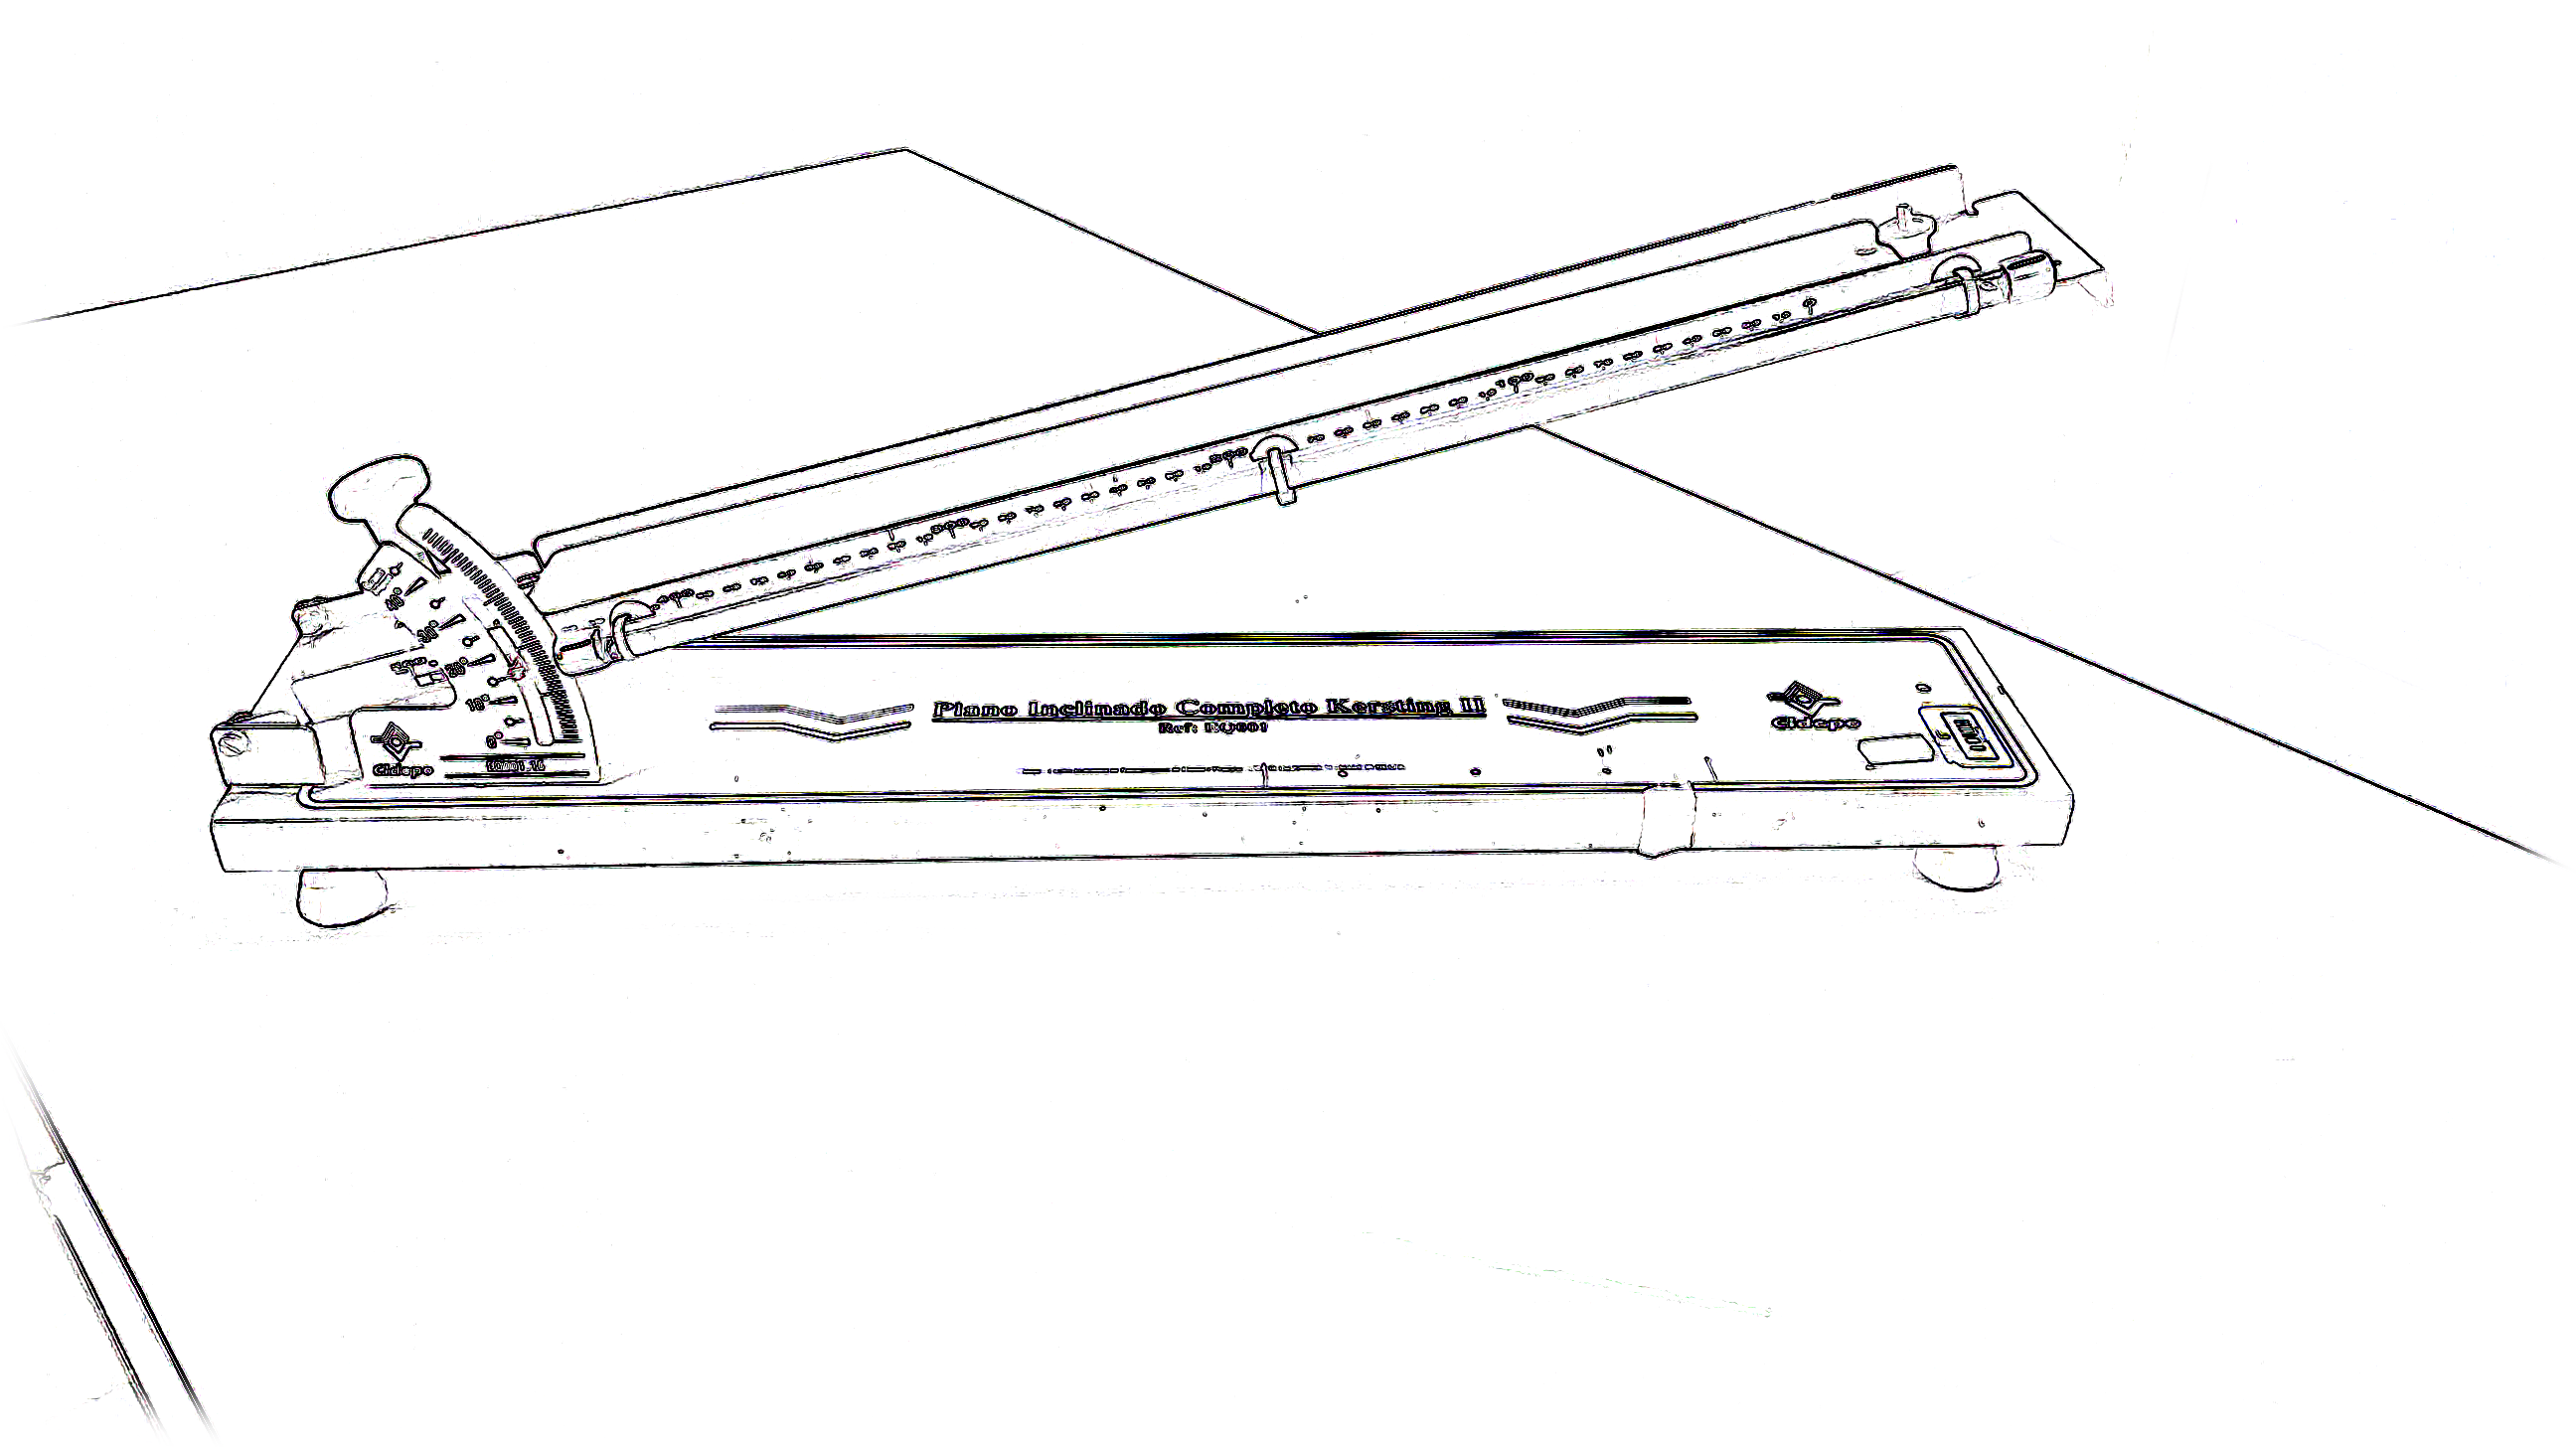
\includegraphics[width=\linewidth]{Ilustrations/Arrasto.png}
\caption{Plano inclinado com tubo preenchido com um fluido viscoso.}
\end{marginfigure}

%%%%%%%%%%%%%%%%%%%%%%%%%%%%%%%%%%%%%%%%%%%%%%%%%%%%%%%%%%%%%%%%%%%%%
\paragraph{MRU -- Deslocamento da esfera no tubo com fluido viscoso:}
%%%%%%%%%%%%%%%%%%%%%%%%%%%%%%%%%%%%%%%%%%%%%%%%%%%%%%%%%%%%%%%%%%%%%

\begin{enumerate}
	\item Ajuste o plano inclinado para um ângulo de \np[\tcdegree]{20,0};
	\item Com um imã, atraia a esfera para a parte superior antes da posição \np[cm]{0,0};\label{Item:Coleta1}
	\item Zere o cronômetro;
	\item Solte a esfera e inicie o cronômetro quando a ela passar pela posição \np[cm]{0,0}. Pare o cronômetro quando a ela passar pela posição final \np[cm]{10,0}. Anote os valores da posição inicial, final, e o tempo registrado pelo cronômetro na Tabela~\ref{DadosMRU};
	\item Repita este procedimento para os seguintes valores de posição final: \np[cm]{15}, \np[cm]{20}, \np[cm]{25}, \np[cm]{30}, \np[cm]{35}, \np[cm]{40}. A cada medida, anote os valores da posição inicial, final, e o tempo registrado pelo cronômetro na Tabela~\ref{DadosMRU};\label{Item:ColetaUltima}
	\item Ajuste o plano inclinado para um ângulo de \degree{40};
	\item Repita os procedimentos do itens \ref{Item:Coleta1} a \ref{Item:ColetaUltima} e anote os dados obtidos na Tabela~\ref{DadosMRU2}.
\end{enumerate}

%%%%%%%%%%%%%%%%%%%%%%%%%%%%%%%%%%%%%%%%%%%%
\paragraph{MRUV -- Queda livre:}
%%%%%%%%%%%%%%%%%%%%%%%%%%%%%%%%%%%%%%%%%%%%

\begin{enumerate}
    \item Ligue o cronômetro através do botão na parte de trás do aparelho;
    \item Certifique-se de que o cronômetro esteja operando na função \texttt{F1} e que o potenciômetro na parte de trás esteja no menor valor de potência que é capaz de prender a esfera;
    \item Ligue o eletroímã através do disjuntor;
	\item Prenda a esfera no eletroímã;
	\item Posicione o sensor superior de forma que ele fique muito próximo de ativar o cronômetro (erga o sensor com o cronômetro ligado e, quando o sensor ativar, desça um pouco, afixando sua posição). Verifique a posição\footnote{Use a escala do próprio suporte vertical do aparato.} inicial do sensor e a anote na Tabela~\ref{DadosMRUV};
	\item Posicione o sensor inferior \np[cm]{5,00} abaixo do primeiro e anote o valor de sua posição\footnote{Novamente, use a escala do próprio suporte vertical do aparato.} na Tabela~\ref{DadosMRUV};
	\item Certifique-se de que o cronômetro esteja zerado;
	\item Desligue o eletroímã e anote o valor do tempo registrado pelo cronômetro para a passagem da esfera na Tabela~\ref{DadosMRUV};
	\item Repita a medida de tempo mais duas vezes, anotando os resultados;
	\item Desloque o sensor inferior mais \np[cm]{5,0} anotando o valor de sua nova posição na Tabela~\ref{DadosMRUV};\label{ItemLoopMRUV}
	\item Ligue o eletroímã através do disjuntor e prenda nele a esfera;
	\item Zere o cronômetro;
	\item Desligue o eletroímã e anote o valor do tempo registrado pelo cronômetro para a passagem da esfera na Tabela~\ref{DadosMRUV}, repetindo a medida mais duas vezes e anotando os resultados;
	\item Repita os itens a partir do item \ref{ItemLoopMRUV} até completar a Tabela~\ref{DadosMRUV} ou não ser mais possível deslocar o sensor inferior.
\end{enumerate}

%%%%%%%%%%%%%%%%%%%%%%%%%%%%%%%%%%%%%%%%%%%%%%%%%%%%%%%%%%%%%%%%%%%%%%%%%%%%%%%
%%%%%%%%%%%%%%%%%%%%%%%%%%%%%%%%%%%%%%%%%%%%%%%%%%%%%%%%%%%%%%%%%%%%%%%%%%%%%%%
%%%%%%%%%%%%%%%%%%%%%%%%%%%%%%%%%%%%%%%%%%%%%%%%%%%%%%%%%%%%%%%%%%%%%%%%%%%%%%%
%%%%%%%%%%%%%%%%%%%%%%%%%%%%%%%%%%%%%%%%%%%%%%%%%%%%%%%%%%%%%%%%%%%%%%%%%%%%%%%
\cleardoublepage

\noindent{}{\huge\textit{Movimento retilíneo uniforme (MRU) e uniformemente variado (MRUV)}}

\vspace{15mm}

\begin{fullwidth}
\noindent{}\makebox[0.6\linewidth]{Turma:\enspace\hrulefill}\makebox[0.4\textwidth]{  Data:\enspace\hrulefill}
\vspace{5mm}

\noindent{}\makebox[0.6\linewidth]{Aluno(a):\enspace\hrulefill}\makebox[0.4\textwidth]{  Matrícula:\enspace\hrulefill}

\noindent{}\makebox[0.6\linewidth]{Aluno(a):\enspace\hrulefill}\makebox[0.4\textwidth]{  Matrícula:\enspace\hrulefill}

\noindent{}\makebox[0.6\linewidth]{Aluno(a):\enspace\hrulefill}\makebox[0.4\textwidth]{  Matrícula:\enspace\hrulefill}

\noindent{}\makebox[0.6\linewidth]{Aluno(a):\enspace\hrulefill}\makebox[0.4\textwidth]{  Matrícula:\enspace\hrulefill}

\noindent{}\makebox[0.6\linewidth]{Aluno(a):\enspace\hrulefill}\makebox[0.4\textwidth]{  Matrícula:\enspace\hrulefill}
\end{fullwidth}

\vspace{5mm}

%%%%%%%%%%%%%%%%%%%%%%%%%%%%%%%%%%%%%%%%%%%%%%%%%%%%%%%%%%%%%%%%%%%%%%%%%%%%%%%
\section{Questionário}
%%%%%%%%%%%%%%%%%%%%%%%%%%%%%%%%%%%%%%%%%%%%%%%%%%%%%%%%%%%%%%%%%%%%%%%%%%%%%%%

\begin{question}[type={exam}]{1}
Apresente os resultados de maneira clara e organizada. Mostre os cálculos requisitados de maneira clara e sucinta, evidenciando o raciocínio desenvolvido.
\end{question}

\begin{question}[type={exam}]{2}
Preencha as colunas de dados experimentais das tabelas com o número adequado de algarismos significativos e unidades.
\end{question}

\begin{question}[type={exam}]{1.5}
Calcule o deslocamento $\Delta x$, o tempo médio $\mean{t}$, e a velocidade para dos dados das Tabelas~\ref{DadosMRU} e~\ref{DadosMRU2}. Observe o número adequado de algarismos significativos e unidades.
\end{question}

\begin{question}[type={exam}]{2}
Para os dados das Tabelas~\ref{DadosMRU} e~\ref{DadosMRU2}, elabore em papel milimetrado um gráfico $x \times \mean{t}$, ou seja, da \emph{distância} percorrida pela esfera contida no tubo do plano inclinado em função do valor médio de \emph{tempo} (isto é, com a distância no eixo $y$ e o tempo no eixo $x$).\footnote{Note que a variável independente em nosso experimento é o deslocamento, sendo que deveríamos colocá-la no eixo horizontal, enquanto o tempo é nossa variável dependente e deveria estar no eixo vertical. Para fins didáticos, no entanto, vamos inverter essa relação para obter um gráfico mais usual.} Note que os dois conjuntos de dados devem ser representados no mesmo gráfico.
\end{question}

\begin{question}[type={exam}]{1.5}
Calcule o o deslocamento $\Delta x$ e o tempo médio $\mean{t}$ para os dados da Tabela~\ref{DadosMRUV}. Considerando que a velocidade inicial da esfera no movimento de queda livre é nula, calcule a aceleração da gravidade. Observe o número adequado de algarismos significativos e unidades.
\end{question}

\begin{question}[type={exam}]{2}
Para os dados da Tabela~\ref{DadosMRUV}, elabore em papel milimetrado um gráfico $x \times \mean{t}$, ou seja, um gráfico da \emph{distância} percorrida pela esfera em queda livre em função dos valores médios de \emph{tempo}.\footnote{Novamente, a variável independente é o deslocamento e deveria estar no eixo horizontal, enquanto o tempo é a variável dependente e deveria estar no eixo vertical. Para fins didáticos, vamos inverter essa relação para obter um gráfico mais usual.}
\end{question}
\vfill
%%%%%%%%%%%%%%%%%%%%%%%%%%%%%%%%%%%%%%%%%%%%%%%%%%%%%%%%%%%%%%%%%%%%%%%%%%%%%%%
\pagebreak
\section{Tabelas}
%%%%%%%%%%%%%%%%%%%%%%%%%%%%%%%%%%%%%%%%%%%%%%%%%%%%%%%%%%%%%%%%%%%%%%%%%%%%%%%

\begin{table*}[!ht]
\centering
\begin{tabular}{lp{25mm}p{25mm}p{25mm}p{25mm}p{25mm}l}
\toprule
	&\multicolumn{4}{l}{\textbf{Dados Experimentais}} \\
	\cmidrule{2-6}
	& $x_0$ & $x_f$ & $t_1$ & $t_2$ & $t_3$ & \\
	\cmidrule{2-6}
	& \cellcolor[gray]{0.89} & \cellcolor[gray]{0.92} & \cellcolor[gray]{0.89} & \cellcolor[gray]{0.92} & \cellcolor[gray]{0.89} \\
	& \cellcolor[gray]{0.95} & \cellcolor[gray]{0.97} & \cellcolor[gray]{0.95} & \cellcolor[gray]{0.97} & \cellcolor[gray]{0.95} \\
	& \cellcolor[gray]{0.89} & \cellcolor[gray]{0.92} & \cellcolor[gray]{0.89} & \cellcolor[gray]{0.92} & \cellcolor[gray]{0.89} \\
	& \cellcolor[gray]{0.95} & \cellcolor[gray]{0.97} & \cellcolor[gray]{0.95} & \cellcolor[gray]{0.97} & \cellcolor[gray]{0.95} \\
	& \cellcolor[gray]{0.89} & \cellcolor[gray]{0.92} & \cellcolor[gray]{0.89} & \cellcolor[gray]{0.92} & \cellcolor[gray]{0.89} \\
	& \cellcolor[gray]{0.95} & \cellcolor[gray]{0.97} & \cellcolor[gray]{0.95} & \cellcolor[gray]{0.97} & \cellcolor[gray]{0.95} \\
	& \cellcolor[gray]{0.89} & \cellcolor[gray]{0.92} & \cellcolor[gray]{0.89} & \cellcolor[gray]{0.92} & \cellcolor[gray]{0.89} \\
	& \cellcolor[gray]{0.95} & \cellcolor[gray]{0.97} & \cellcolor[gray]{0.95} & \cellcolor[gray]{0.97} & \cellcolor[gray]{0.95} \\
	& \cellcolor[gray]{0.89} & \cellcolor[gray]{0.92} & \cellcolor[gray]{0.89} & \cellcolor[gray]{0.92} & \cellcolor[gray]{0.89} \\
	& \cellcolor[gray]{0.95} & \cellcolor[gray]{0.97} & \cellcolor[gray]{0.95} & \cellcolor[gray]{0.97} & \cellcolor[gray]{0.95} \\
	\cmidrule{2-6}
\\
	& \multicolumn{3}{l}{\textbf{Dados calculados}} \\
	\cmidrule{2-4}
	& $\Delta x$ & $\mean{t}$ & $v = \Delta x / \mean{t}$ \\
	\cmidrule{2-4}
	& \cellcolor[gray]{0.89} & \cellcolor[gray]{0.92} & \cellcolor[gray]{0.89} \\ 
	& \cellcolor[gray]{0.95} & \cellcolor[gray]{0.97} & \cellcolor[gray]{0.95} \\ 
	& \cellcolor[gray]{0.89} & \cellcolor[gray]{0.92} & \cellcolor[gray]{0.89} \\ 
	& \cellcolor[gray]{0.95} & \cellcolor[gray]{0.97} & \cellcolor[gray]{0.95} \\ 
	& \cellcolor[gray]{0.89} & \cellcolor[gray]{0.92} & \cellcolor[gray]{0.89} \\ 
	& \cellcolor[gray]{0.95} & \cellcolor[gray]{0.97} & \cellcolor[gray]{0.95} \\ 
	& \cellcolor[gray]{0.89} & \cellcolor[gray]{0.92} & \cellcolor[gray]{0.89} \\ 
	& \cellcolor[gray]{0.95} & \cellcolor[gray]{0.97} & \cellcolor[gray]{0.95} \\ 
	& \cellcolor[gray]{0.89} & \cellcolor[gray]{0.92} & \cellcolor[gray]{0.89} \\ 
	& \cellcolor[gray]{0.95} & \cellcolor[gray]{0.97} & \cellcolor[gray]{0.95} \\ 
	\cmidrule{2-4}
\bottomrule
\end{tabular}
\caption[][5mm]{Valores de tempo e deslocamento para o MRU para o ângulo de \degree{20}.}
\label{DadosMRU}
\end{table*}

\begin{table*}[!ht]
\centering
\begin{tabular}{lp{25mm}p{25mm}p{25mm}p{25mm}p{25mm}l}
\toprule
	&\multicolumn{4}{l}{\textbf{Dados Experimentais}} \\
	\cmidrule{2-6}
	& $x_0$ & $x_f$ & $t_1$ & $t_2$ & $t_3$ & \\
	\cmidrule{2-6}
	& \cellcolor[gray]{0.89} & \cellcolor[gray]{0.92} & \cellcolor[gray]{0.89} & \cellcolor[gray]{0.92} & \cellcolor[gray]{0.89} \\
	& \cellcolor[gray]{0.95} & \cellcolor[gray]{0.97} & \cellcolor[gray]{0.95} & \cellcolor[gray]{0.97} & \cellcolor[gray]{0.95} \\
	& \cellcolor[gray]{0.89} & \cellcolor[gray]{0.92} & \cellcolor[gray]{0.89} & \cellcolor[gray]{0.92} & \cellcolor[gray]{0.89} \\
	& \cellcolor[gray]{0.95} & \cellcolor[gray]{0.97} & \cellcolor[gray]{0.95} & \cellcolor[gray]{0.97} & \cellcolor[gray]{0.95} \\
	& \cellcolor[gray]{0.89} & \cellcolor[gray]{0.92} & \cellcolor[gray]{0.89} & \cellcolor[gray]{0.92} & \cellcolor[gray]{0.89} \\
	& \cellcolor[gray]{0.95} & \cellcolor[gray]{0.97} & \cellcolor[gray]{0.95} & \cellcolor[gray]{0.97} & \cellcolor[gray]{0.95} \\
	& \cellcolor[gray]{0.89} & \cellcolor[gray]{0.92} & \cellcolor[gray]{0.89} & \cellcolor[gray]{0.92} & \cellcolor[gray]{0.89} \\
	& \cellcolor[gray]{0.95} & \cellcolor[gray]{0.97} & \cellcolor[gray]{0.95} & \cellcolor[gray]{0.97} & \cellcolor[gray]{0.95} \\
	& \cellcolor[gray]{0.89} & \cellcolor[gray]{0.92} & \cellcolor[gray]{0.89} & \cellcolor[gray]{0.92} & \cellcolor[gray]{0.89} \\
	& \cellcolor[gray]{0.95} & \cellcolor[gray]{0.97} & \cellcolor[gray]{0.95} & \cellcolor[gray]{0.97} & \cellcolor[gray]{0.95} \\
	\cmidrule{2-6}
\\
	& \multicolumn{3}{l}{\textbf{Dados calculados}} \\
	\cmidrule{2-4}
	& $\Delta x$ & $\mean{t}$ & $v = \Delta x / \mean{t}$ \\
	\cmidrule{2-4}
	& \cellcolor[gray]{0.89} & \cellcolor[gray]{0.92} & \cellcolor[gray]{0.89} \\ 
	& \cellcolor[gray]{0.95} & \cellcolor[gray]{0.97} & \cellcolor[gray]{0.95} \\ 
	& \cellcolor[gray]{0.89} & \cellcolor[gray]{0.92} & \cellcolor[gray]{0.89} \\ 
	& \cellcolor[gray]{0.95} & \cellcolor[gray]{0.97} & \cellcolor[gray]{0.95} \\ 
	& \cellcolor[gray]{0.89} & \cellcolor[gray]{0.92} & \cellcolor[gray]{0.89} \\ 
	& \cellcolor[gray]{0.95} & \cellcolor[gray]{0.97} & \cellcolor[gray]{0.95} \\ 
	& \cellcolor[gray]{0.89} & \cellcolor[gray]{0.92} & \cellcolor[gray]{0.89} \\ 
	& \cellcolor[gray]{0.95} & \cellcolor[gray]{0.97} & \cellcolor[gray]{0.95} \\ 
	& \cellcolor[gray]{0.89} & \cellcolor[gray]{0.92} & \cellcolor[gray]{0.89} \\ 
	& \cellcolor[gray]{0.95} & \cellcolor[gray]{0.97} & \cellcolor[gray]{0.95} \\ 
	\cmidrule{2-4}
\bottomrule
\end{tabular}
\caption[][5mm]{Valores de tempo e deslocamento para o MRU para o ângulo de \degree{40}.}
\label{DadosMRU2}
\end{table*}

\begin{table*}[!ht]
\centering
\begin{tabular}{lp{25mm}p{25mm}p{25mm}p{25mm}p{25mm}l}
\toprule
	&\multicolumn{4}{l}{\textbf{Dados Experimentais}} \\
	\cmidrule{2-6}
	& $x_0$ & $x_f$ & $t_1$ & $t_2$ & $t_3$ & \\
	\cmidrule{2-6}
	& \cellcolor[gray]{0.89} & \cellcolor[gray]{0.92} & \cellcolor[gray]{0.89} & \cellcolor[gray]{0.92} & \cellcolor[gray]{0.89} \\
	& \cellcolor[gray]{0.95} & \cellcolor[gray]{0.97} & \cellcolor[gray]{0.95} & \cellcolor[gray]{0.97} & \cellcolor[gray]{0.95} \\
	& \cellcolor[gray]{0.89} & \cellcolor[gray]{0.92} & \cellcolor[gray]{0.89} & \cellcolor[gray]{0.92} & \cellcolor[gray]{0.89} \\
	& \cellcolor[gray]{0.95} & \cellcolor[gray]{0.97} & \cellcolor[gray]{0.95} & \cellcolor[gray]{0.97} & \cellcolor[gray]{0.95} \\
	& \cellcolor[gray]{0.89} & \cellcolor[gray]{0.92} & \cellcolor[gray]{0.89} & \cellcolor[gray]{0.92} & \cellcolor[gray]{0.89} \\
	& \cellcolor[gray]{0.95} & \cellcolor[gray]{0.97} & \cellcolor[gray]{0.95} & \cellcolor[gray]{0.97} & \cellcolor[gray]{0.95} \\
	& \cellcolor[gray]{0.89} & \cellcolor[gray]{0.92} & \cellcolor[gray]{0.89} & \cellcolor[gray]{0.92} & \cellcolor[gray]{0.89} \\
	& \cellcolor[gray]{0.95} & \cellcolor[gray]{0.97} & \cellcolor[gray]{0.95} & \cellcolor[gray]{0.97} & \cellcolor[gray]{0.95} \\
	& \cellcolor[gray]{0.89} & \cellcolor[gray]{0.92} & \cellcolor[gray]{0.89} & \cellcolor[gray]{0.92} & \cellcolor[gray]{0.89} \\
	& \cellcolor[gray]{0.95} & \cellcolor[gray]{0.97} & \cellcolor[gray]{0.95} & \cellcolor[gray]{0.97} & \cellcolor[gray]{0.95} \\
	\cmidrule{2-6}
\\
	& \multicolumn{3}{l}{\textbf{Dados calculados}} \\
	\cmidrule{2-4}
	& $\Delta x$ & $\mean{t}$ & $g = 2 \Delta x / \mean{t}^2$ \\
	\cmidrule{2-4}
	& \cellcolor[gray]{0.89} & \cellcolor[gray]{0.92} & \cellcolor[gray]{0.89} \\ 
	& \cellcolor[gray]{0.95} & \cellcolor[gray]{0.97} & \cellcolor[gray]{0.95} \\ 
	& \cellcolor[gray]{0.89} & \cellcolor[gray]{0.92} & \cellcolor[gray]{0.89} \\ 
	& \cellcolor[gray]{0.95} & \cellcolor[gray]{0.97} & \cellcolor[gray]{0.95} \\ 
	& \cellcolor[gray]{0.89} & \cellcolor[gray]{0.92} & \cellcolor[gray]{0.89} \\ 
	& \cellcolor[gray]{0.95} & \cellcolor[gray]{0.97} & \cellcolor[gray]{0.95} \\ 
	& \cellcolor[gray]{0.89} & \cellcolor[gray]{0.92} & \cellcolor[gray]{0.89} \\ 
	& \cellcolor[gray]{0.95} & \cellcolor[gray]{0.97} & \cellcolor[gray]{0.95} \\ 
	& \cellcolor[gray]{0.89} & \cellcolor[gray]{0.92} & \cellcolor[gray]{0.89} \\ 
	& \cellcolor[gray]{0.95} & \cellcolor[gray]{0.97} & \cellcolor[gray]{0.95} \\ 
	\cmidrule{2-4}
\bottomrule
\end{tabular}
\caption[][5mm]{Dados do MRUV}
\label{DadosMRUV}
\end{table*}


%%%%%%%%%%%%%%%%%%%%%%%%%%%%%%%%%%%%%%%%%%%%%%%%%%%%%%%%%%%%%%%%%%%%%%%%%%%%%%%%
\chapter{Lançamento Oblíquo} % Sem "Experiência 01" ou qualquer outro número
\label{Chap:LancamentoObliquo}        % para poder trocar a ordem com facilidade
%%%%%%%%%%%%%%%%%%%%%%%%%%%%%%%%%%%%%%%%%%%%%%%%%%%%%%%%%%%%%%%%%%%%%%%%%%%%%%%

\begin{fullwidth}
	Que experimento faremos?
	Qual é o objetivo?
	O que veremos/revisaremos? (teoria física)
	Quais conceitos/técnicas de análise de dados utilizaremos?
	\comment{A ideia é introduzir erros com essa experiência. Podemos usar medidas, algarismos sig., gráficos, erros (escala, prop)}
\end{fullwidth}

%%%%%%%%%%%%%%%%%%%%%%%%%%%%%%%%%%%%%%%%%%%%%%%%%%%%%%%%%%%%%%%%%%%%%%%%%%%%%%%
\section{Física do experimento}
%%%%%%%%%%%%%%%%%%%%%%%%%%%%%%%%%%%%%%%%%%%%%%%%%%%%%%%%%%%%%%%%%%%%%%%%%%%%%%%

%%%%%%%%%%%%%%%%%%%%%%%%%%%%%%%%%%%%%%%%%%%%%
%\subsection{Se necessário, usar subsections}
%%%%%%%%%%%%%%%%%%%%%%%%%%%%%%%%%%%%%%%%%%%%%

%%%%%%%%%%%%%%%%%%%%%%%%%%%%%%%%%%%%%%%%%%%%%%%%%%%%%%%%%%%%%%%%%%%%%%%%%%%%%%%
\section{Experimento}
%%%%%%%%%%%%%%%%%%%%%%%%%%%%%%%%%%%%%%%%%%%%%%%%%%%%%%%%%%%%%%%%%%%%%%%%%%%%%%%

%%%%%%%%%%%%%%%%%%%%%%
\subsection{Objetivos}
%%%%%%%%%%%%%%%%%%%%%%

\begin{itemize}
	\item Resultados concretos que devemos conseguir;
	\item Observar a relação de tal coisa com outra coisa;
	\item Calcular a constante $x$.
\end{itemize}

%%%%%%%%%%%%%%%%%%%%%%%%%%%%%%%%%%%%%%%%%%%%%%%%%%%%%%%%%%%%%%%%%%%%%%%%%%%%%%%
\section{Material Necessário}
%%%%%%%%%%%%%%%%%%%%%%%%%%%%%%%%%%%%%%%%%%%%%%%%%%%%%%%%%%%%%%%%%%%%%%%%%%%%%%%

\begin{itemize}
	\item Item 1;
	\item Item 2.
\end{itemize}

%%%%%%%%%%%%%%%%%%%%%%%%%%%%%%%%%%%%%%%%%%%%%%%%%%%%%%%%%%%%%%%%%%%%%%%%%%%%%%%
\section{Procedimento Experimental}
%%%%%%%%%%%%%%%%%%%%%%%%%%%%%%%%%%%%%%%%%%%%%%%%%%%%%%%%%%%%%%%%%%%%%%%%%%%%%%%

%%%%%%%%%%%%%%%%%%%%%
%\subsection{Parte A} % Se necessário
%%%%%%%%%%%%%%%%%%%%%
\begin{enumerate}
	\item Passo 1;
	\item Passo 2;
	\item Passo 3.
\end{enumerate}

%%%%%%%%%%%%%%%%%%%%%%%%%%%%%%%%%%%%%%%%%%%%%%%%%%%%%%%%%%%%%%%%%%%%%%%%%%%%%%%
%%%%%%%%%%%%%%%%%%%%%%%%%%%%%%%%%%%%%%%%%%%%%%%%%%%%%%%%%%%%%%%%%%%%%%%%%%%%%%%
%%%%%%%%%%%%%%%%%%%%%%%%%%%%%%%%%%%%%%%%%%%%%%%%%%%%%%%%%%%%%%%%%%%%%%%%%%%%%%%
%%%%%%%%%%%%%%%%%%%%%%%%%%%%%%%%%%%%%%%%%%%%%%%%%%%%%%%%%%%%%%%%%%%%%%%%%%%%%%%
\cleardoublepage

\noindent{}{\huge\textit{Lançamento Obliquo}}

\vspace{15mm}

\begin{fullwidth}
\noindent{}\makebox[0.6\linewidth]{Turma:\enspace\hrulefill}\makebox[0.4\textwidth]{  Data:\enspace\hrulefill}
\vspace{5mm}

\noindent{}\makebox[0.6\linewidth]{Aluno(a):\enspace\hrulefill}\makebox[0.4\textwidth]{  Matrícula:\enspace\hrulefill}

\noindent{}\makebox[0.6\linewidth]{Aluno(a):\enspace\hrulefill}\makebox[0.4\textwidth]{  Matrícula:\enspace\hrulefill}

\noindent{}\makebox[0.6\linewidth]{Aluno(a):\enspace\hrulefill}\makebox[0.4\textwidth]{  Matrícula:\enspace\hrulefill}

\noindent{}\makebox[0.6\linewidth]{Aluno(a):\enspace\hrulefill}\makebox[0.4\textwidth]{  Matrícula:\enspace\hrulefill}

\noindent{}\makebox[0.6\linewidth]{Aluno(a):\enspace\hrulefill}\makebox[0.4\textwidth]{  Matrícula:\enspace\hrulefill}
\end{fullwidth}

\vspace{5mm}

%%%%%%%%%%%%%%%%%%%%%%%%%%%%%%%%%%%%%%%%%%%%%%%%%%%%%%%%%%%%%%%%%%%%%%%%%%%%%%%
\section{Questionário}
%%%%%%%%%%%%%%%%%%%%%%%%%%%%%%%%%%%%%%%%%%%%%%%%%%%%%%%%%%%%%%%%%%%%%%%%%%%%%%%
\emph{Nas questões seguintes, apresente os cálculos requisitados de maneira clara e sucinta, para que o professor possa acompanhar o raciocínio desenvolvido.}
\vspace{5mm}

\begin{question}[type={exam}]{2}
Lorem ipsum dolor sit amet, consectetuer adi-
piscing elit. Ut purus elit, vestibulum ut, placerat ac, adipiscing vitae,
felis. Curabitur dictum gravida mauris. Nam arcu libero, nonummy
eget, consectetuer id, vulputate a, magna. Donec vehicula augue
eu neque. Pellentesque habitant morbi tristique senectus et netus
et malesuada fames ac turpis egestas. Mauris ut leo. Cras viverra
metus rhoncus sem. Nulla et lectus vestibulum urna fringilla ultrices.
\end{question}

\begin{question}[type={exam}]{2}
Lorem ipsum dolor sit amet, consectetuer adi-
piscing elit. Ut purus elit, vestibulum ut, placerat ac, adipiscing vitae,
felis. Curabitur dictum gravida mauris. Nam arcu libero, nonummy
eget, consectetuer id, vulputate a, magna. Donec vehicula augue
eu neque. Pellentesque habitant morbi tristique senectus et netus
et malesuada fames ac turpis egestas. Mauris ut leo. Cras viverra
metus rhoncus sem. Nulla et lectus vestibulum urna fringilla ultrices.
\end{question}

\begin{question}[type={exam}]{2}
Lorem ipsum dolor sit amet, consectetuer adi-
piscing elit. Ut purus elit, vestibulum ut, placerat ac, adipiscing vitae,
felis. Curabitur dictum gravida mauris. Nam arcu libero, nonummy
eget, consectetuer id, vulputate a, magna. Donec vehicula augue
eu neque. Pellentesque habitant morbi tristique senectus et netus
et malesuada fames ac turpis egestas. Mauris ut leo. Cras viverra
metus rhoncus sem. Nulla et lectus vestibulum urna fringilla ultrices.
\end{question}

\begin{question}[type={exam}]{2}
Lorem ipsum dolor sit amet, consectetuer adi-
piscing elit. Ut purus elit, vestibulum ut, placerat ac, adipiscing vitae,
felis. Curabitur dictum gravida mauris. Nam arcu libero, nonummy
eget, consectetuer id, vulputate a, magna. Donec vehicula augue
eu neque. Pellentesque habitant morbi tristique senectus et netus
et malesuada fames ac turpis egestas. Mauris ut leo. Cras viverra
metus rhoncus sem. Nulla et lectus vestibulum urna fringilla ultrices.
\end{question}

\begin{question}[type={exam}]{2}
Lorem ipsum dolor sit amet, consectetuer adi-
piscing elit. Ut purus elit, vestibulum ut, placerat ac, adipiscing vitae,
felis. Curabitur dictum gravida mauris. Nam arcu libero, nonummy
eget, consectetuer id, vulputate a, magna. Donec vehicula augue
eu neque. Pellentesque habitant morbi tristique senectus et netus
et malesuada fames ac turpis egestas. Mauris ut leo. Cras viverra
metus rhoncus sem. Nulla et lectus vestibulum urna fringilla ultrices.
\end{question}
\vfill
%%%%%%%%%%%%%%%%%%%%%%%%%%%%%%%%%%%%%%%%%%%%%%%%%%%%%%%%%%%%%%%%%%%%%%%%%%%%%%%
\pagebreak
\section{Tabelas}
%%%%%%%%%%%%%%%%%%%%%%%%%%%%%%%%%%%%%%%%%%%%%%%%%%%%%%%%%%%%%%%%%%%%%%%%%%%%%%%


%%%%%%%%%%%%%%%%%%%%%%%%%%%%%%%%%%%%%%%%%%%%%%%%%%%%%%%%%%%%%%%%%%%%%%%%%%%%%%%%
\chapter{Lei de Hooke}
\label{Chap:ExpLeiDeHooke}
%%%%%%%%%%%%%%%%%%%%%%%%%%%%%%%%%%%%%%%%%%%%%%%%%%%%%%%%%%%%%%%%%%%%%%%%%%%%%%%

\begin{fullwidth}\it
	Realizaremos um experimento em que submeteremos uma mola a forças com intensidades diferentes, observando as distensões correspondentes. Procuramos assim observar experimentalmente a Lei de Hooke --- que afirma que as distensões são diretamente proporcionais à intensidade da força aplicada ---. Utilizaremos os seguintes conceitos: medidas, algarismos significativos, gráficos, e regressão linear.
\end{fullwidth}

%%%%%%%%%%%%%%%%%%%%%%%%%%%%%%%%%%%%%%%%%%%%%%%%
\section[Linhas de tendência e regressão linear]{Linhas de tendência e regressão linear\footnote{Esta seção é um resumo do Capítulo~\ref{Chap:RegressoLinear}.}}
%%%%%%%%%%%%%%%%%%%%%%%%%%%%%%%%%%%%%%%%%%%%%%%%

Quando realizamos um experimento, procuramos relacionar uma variável dependente a uma variável independente. Para visualizarmos a relação entre as duas, é interessante fazer uma representação gráfica da variável dependente em função dos valores da variável independente. Podemos assim verificar uma tendência geral dos pontos, que pode seguir padrões retilíneos, parabólicos, etc. Muitas vezes tal padrão é muito claro, pois os pontos tem uma \emph{dispersão} baixa. Outras vezes a dispersão é razoavelmente alta e fica difícil verificar o padrão seguido pelos pontos.

Mesmo em casos em que podemos verificar um padrão aparente ao fazer um gráfico, determinar a forma mais adequada para a \emph{linha de tendência} que melhor descreve os pontos experimentais ---~ou mesmo afirmar que tais pontos seguem este padrão~--- pode ser complicado. Se, por exemplo, fizermos uma série de medidas que seguem um padrão parabólico, mas com medidas que se restringem a um intervalo pequeno da variável independente, o gráfico terá a aparência de uma reta.

Determinar o padrão seguido pelos pontos, é, portanto, uma tarefa que não pode ser feita a partir de um gráfico: o mais adequado é termos uma \emph{teoria acerca do fenômeno físico} que descreva qual é o padrão que os pontos devem seguir, e usar um gráfico para determinar se tal descrição é coerente. Verificaremos posteriormente como determinar se uma teoria é plausível ou não, por hora vamos nos preocupar em determinar a \emph{melhor reta} que ajusta um conjunto de dados.

Sempre que tivermos um conjunto de dados, podemos calcular a melhor reta que o representa através de um processo de \emph{regressão linear}. Este processo consiste em aplicar um método matemático que tome os dados experimentais e calcule os coeficientes linear $A$ e angular $B$ para a equação da reta:
\begin{equation}
	y = A + Bx.
\end{equation}

%%%%%%%%%%%%%%%%%%%%%%%%%%%%%
\paragraph{Mínimos quadrados}
%%%%%%%%%%%%%%%%%%%%%%%%%%%%%

O método utilizado para obter tais coeficientes é o de \emph{mínimos quadrados}. Nele, são encontrados os coeficientes de forma a minimizar o quadrado da distância entre os pontos experimentais e a ``melhor reta''. É possível mostrar\cite{Taylor}, utilizando técnicas de cálculo, que para minimizarmos a soma do quadrado das distâncias entre os pontos e a melhor reta, os coeficientes linear e angular são dados por
\begin{align}
	A &= \frac{\sum x_i^2 \sum y_i - \sum x_i \sum x_iy_i}{N \sum x_i^2 - (\sum x_i)^2} \\
	B &= \frac{N\sum x_iy_i - \sum x_i \sum y_i}{N \sum x_i^2 - (\sum x_i)^2}.
\end{align}
%
onde as somas se dão sobre todas mas medidas $x_i$ e $y_i$, $N$ representa o número de medidas, e as médias das medidas para as variáveis $x$ e $y$ são representadas por $\mean{x}$ e $\mean{y}$, respectivamente. Após fazer a regressão, podemos utilizar os coeficientes para traçar as \emph{retas de tendência} nos gráficos\footnote{Quando tais retas forem calculadas, adicione as equações resultantes aos gráficos.}.

Ao fazermos o processo de regressão linear, a calculadora também calculará o \emph{coeficiente de correlação linear} $r$, dado por
\begin{equation}
	r = \frac{\sum (x_i - \mean{x})(y_i-\mean{y})}{\sqrt{\sum(x_i - \mean{x})^2\sum (y_i - \mean{y})^2}}.
\end{equation}
%
Tal coeficiente pode ser interpretado como um ``índice de confiança'' e geralmente é calculado ao quadrado, pois seus valores podem variar entre $-1$ e $1$. Quanto mais próximo $r$ for de $\pm 1$, menor é a dispersão dos pontos em relação ao comportamento retilíneo, ou seja, maiores são as chances de que o fenômeno estudado e que deu origem aos dados siga uma relação linear. Este número geralmente se parece com algo como $r^2=\np{0,99998}$, $r^2=\np{0,997}$, $r^2= \np{0,990}$, etc., quando os dados são altamente lineares e relativamente abundantes. Se a dispersão em relação ao comportamento linear for grande e forem poucos os pontos, $r^2$ pode cair para \np{0,7}, ou valores menores.

\begin{figure}[!h]
\centering
\begin{tikzpicture}[gnuplot]
%% generated with GNUPLOT 5.0p0 (Lua 5.3; terminal rev. 99, script rev. 100)
%% 2015-05-18T22:58:50 BRT
\path (0.000,0.000) rectangle (14.000,9.000);
\gpcolor{color=gp lt color border}
\gpsetlinetype{gp lt border}
\gpsetdashtype{gp dt solid}
\gpsetlinewidth{1.00}
\draw[gp path] (1.320,2.077)--(1.500,2.077);
\draw[gp path] (13.447,2.077)--(13.267,2.077);
\node[gp node right] at (1.136,2.077) {$20$};
\draw[gp path] (1.320,3.534)--(1.500,3.534);
\draw[gp path] (13.447,3.534)--(13.267,3.534);
\node[gp node right] at (1.136,3.534) {$40$};
\draw[gp path] (1.320,4.990)--(1.500,4.990);
\draw[gp path] (13.447,4.990)--(13.267,4.990);
\node[gp node right] at (1.136,4.990) {$60$};
\draw[gp path] (1.320,6.446)--(1.500,6.446);
\draw[gp path] (13.447,6.446)--(13.267,6.446);
\node[gp node right] at (1.136,6.446) {$80$};
\draw[gp path] (1.320,7.903)--(1.500,7.903);
\draw[gp path] (13.447,7.903)--(13.267,7.903);
\node[gp node right] at (1.136,7.903) {$100$};
\draw[gp path] (1.711,0.985)--(1.711,1.165);
\draw[gp path] (1.711,8.631)--(1.711,8.451);
\node[gp node center] at (1.711,0.677) {$0$};
\draw[gp path] (3.667,0.985)--(3.667,1.165);
\draw[gp path] (3.667,8.631)--(3.667,8.451);
\node[gp node center] at (3.667,0.677) {$5$};
\draw[gp path] (5.623,0.985)--(5.623,1.165);
\draw[gp path] (5.623,8.631)--(5.623,8.451);
\node[gp node center] at (5.623,0.677) {$10$};
\draw[gp path] (7.579,0.985)--(7.579,1.165);
\draw[gp path] (7.579,8.631)--(7.579,8.451);
\node[gp node center] at (7.579,0.677) {$15$};
\draw[gp path] (9.535,0.985)--(9.535,1.165);
\draw[gp path] (9.535,8.631)--(9.535,8.451);
\node[gp node center] at (9.535,0.677) {$20$};
\draw[gp path] (11.491,0.985)--(11.491,1.165);
\draw[gp path] (11.491,8.631)--(11.491,8.451);
\node[gp node center] at (11.491,0.677) {$25$};
\draw[gp path] (13.447,0.985)--(13.447,1.165);
\draw[gp path] (13.447,8.631)--(13.447,8.451);
\node[gp node center] at (13.447,0.677) {$30$};
\draw[gp path] (1.320,8.631)--(1.320,0.985)--(13.447,0.985)--(13.447,8.631)--cycle;
\node[gp node center,rotate=-270] at (0.246,4.808) {$y_1$};
\node[gp node center] at (7.383,0.215) {$x$};
\node[gp node left] at (2.788,8.297) {Dados experimentais};
\gpcolor{rgb color={0.000,0.000,0.000}}
\gpsetlinewidth{2.00}
\gpsetpointsize{4.00}
\gppoint{gp mark 7}{(1.990,1.682)}
\gppoint{gp mark 7}{(2.765,2.128)}
\gppoint{gp mark 7}{(3.428,2.458)}
\gppoint{gp mark 7}{(3.652,2.620)}
\gppoint{gp mark 7}{(4.154,2.823)}
\gppoint{gp mark 7}{(4.558,3.051)}
\gppoint{gp mark 7}{(4.676,3.111)}
\gppoint{gp mark 7}{(4.731,3.222)}
\gppoint{gp mark 7}{(4.806,3.170)}
\gppoint{gp mark 7}{(4.950,3.354)}
\gppoint{gp mark 7}{(5.245,3.577)}
\gppoint{gp mark 7}{(5.405,3.472)}
\gppoint{gp mark 7}{(5.743,3.769)}
\gppoint{gp mark 7}{(5.847,3.709)}
\gppoint{gp mark 7}{(6.084,3.883)}
\gppoint{gp mark 7}{(7.710,4.816)}
\gppoint{gp mark 7}{(8.370,5.269)}
\gppoint{gp mark 7}{(9.115,5.577)}
\gppoint{gp mark 7}{(9.773,6.039)}
\gppoint{gp mark 7}{(9.878,6.088)}
\gppoint{gp mark 7}{(9.963,6.100)}
\gppoint{gp mark 7}{(10.406,6.246)}
\gppoint{gp mark 7}{(10.477,6.523)}
\gppoint{gp mark 7}{(10.501,6.361)}
\gppoint{gp mark 7}{(10.739,6.498)}
\gppoint{gp mark 7}{(12.047,7.279)}
\gppoint{gp mark 7}{(12.220,7.304)}
\gppoint{gp mark 7}{(12.414,7.414)}
\gppoint{gp mark 7}{(2.146,8.297)}
\gpcolor{color=gp lt color border}
\node[gp node left] at (2.788,7.989) {$y(x)=\np{2.9844463644}x + \np{12.141173236}$, $r^2 = \np{0.9989011203}$};
\gpcolor{rgb color={0.000,0.000,0.000}}
\draw[gp path] (1.688,7.989)--(2.604,7.989);
\draw[gp path] (1.908,1.614)--(1.914,1.618)--(1.920,1.621)--(1.926,1.625)--(1.932,1.628)%
  --(1.938,1.631)--(1.945,1.635)--(1.951,1.638)--(1.957,1.641)--(1.963,1.645)--(1.969,1.648)%
  --(1.975,1.651)--(1.981,1.655)--(1.987,1.658)--(1.993,1.662)--(1.999,1.665)--(2.005,1.668)%
  --(2.011,1.672)--(2.017,1.675)--(2.023,1.678)--(2.029,1.682)--(2.035,1.685)--(2.042,1.689)%
  --(2.048,1.692)--(2.054,1.695)--(2.060,1.699)--(2.066,1.702)--(2.072,1.705)--(2.078,1.709)%
  --(2.084,1.712)--(2.090,1.715)--(2.096,1.719)--(2.102,1.722)--(2.108,1.726)--(2.114,1.729)%
  --(2.120,1.732)--(2.126,1.736)--(2.133,1.739)--(2.139,1.742)--(2.145,1.746)--(2.151,1.749)%
  --(2.157,1.753)--(2.163,1.756)--(2.169,1.759)--(2.175,1.763)--(2.181,1.766)--(2.187,1.769)%
  --(2.193,1.773)--(2.199,1.776)--(2.205,1.779)--(2.211,1.783)--(2.217,1.786)--(2.223,1.790)%
  --(2.230,1.793)--(2.236,1.796)--(2.242,1.800)--(2.248,1.803)--(2.254,1.806)--(2.260,1.810)%
  --(2.266,1.813)--(2.272,1.817)--(2.278,1.820)--(2.284,1.823)--(2.290,1.827)--(2.296,1.830)%
  --(2.302,1.833)--(2.308,1.837)--(2.314,1.840)--(2.320,1.843)--(2.327,1.847)--(2.333,1.850)%
  --(2.339,1.854)--(2.345,1.857)--(2.351,1.860)--(2.357,1.864)--(2.363,1.867)--(2.369,1.870)%
  --(2.375,1.874)--(2.381,1.877)--(2.387,1.881)--(2.393,1.884)--(2.399,1.887)--(2.405,1.891)%
  --(2.411,1.894)--(2.417,1.897)--(2.424,1.901)--(2.430,1.904)--(2.436,1.907)--(2.442,1.911)%
  --(2.448,1.914)--(2.454,1.918)--(2.460,1.921)--(2.466,1.924)--(2.472,1.928)--(2.478,1.931)%
  --(2.484,1.934)--(2.490,1.938)--(2.496,1.941)--(2.502,1.945)--(2.508,1.948)--(2.515,1.951)%
  --(2.521,1.955)--(2.527,1.958)--(2.533,1.961)--(2.539,1.965)--(2.545,1.968)--(2.551,1.972)%
  --(2.557,1.975)--(2.563,1.978)--(2.569,1.982)--(2.575,1.985)--(2.581,1.988)--(2.587,1.992)%
  --(2.593,1.995)--(2.599,1.998)--(2.605,2.002)--(2.612,2.005)--(2.618,2.009)--(2.624,2.012)%
  --(2.630,2.015)--(2.636,2.019)--(2.642,2.022)--(2.648,2.025)--(2.654,2.029)--(2.660,2.032)%
  --(2.666,2.036)--(2.672,2.039)--(2.678,2.042)--(2.684,2.046)--(2.690,2.049)--(2.696,2.052)%
  --(2.702,2.056)--(2.709,2.059)--(2.715,2.062)--(2.721,2.066)--(2.727,2.069)--(2.733,2.073)%
  --(2.739,2.076)--(2.745,2.079)--(2.751,2.083)--(2.757,2.086)--(2.763,2.089)--(2.769,2.093)%
  --(2.775,2.096)--(2.781,2.100)--(2.787,2.103)--(2.793,2.106)--(2.799,2.110)--(2.806,2.113)%
  --(2.812,2.116)--(2.818,2.120)--(2.824,2.123)--(2.830,2.126)--(2.836,2.130)--(2.842,2.133)%
  --(2.848,2.137)--(2.854,2.140)--(2.860,2.143)--(2.866,2.147)--(2.872,2.150)--(2.878,2.153)%
  --(2.884,2.157)--(2.890,2.160)--(2.897,2.164)--(2.903,2.167)--(2.909,2.170)--(2.915,2.174)%
  --(2.921,2.177)--(2.927,2.180)--(2.933,2.184)--(2.939,2.187)--(2.945,2.190)--(2.951,2.194)%
  --(2.957,2.197)--(2.963,2.201)--(2.969,2.204)--(2.975,2.207)--(2.981,2.211)--(2.987,2.214)%
  --(2.994,2.217)--(3.000,2.221)--(3.006,2.224)--(3.012,2.228)--(3.018,2.231)--(3.024,2.234)%
  --(3.030,2.238)--(3.036,2.241)--(3.042,2.244)--(3.048,2.248)--(3.054,2.251)--(3.060,2.254)%
  --(3.066,2.258)--(3.072,2.261)--(3.078,2.265)--(3.084,2.268)--(3.091,2.271)--(3.097,2.275)%
  --(3.103,2.278)--(3.109,2.281)--(3.115,2.285)--(3.121,2.288)--(3.127,2.292)--(3.133,2.295)%
  --(3.139,2.298)--(3.145,2.302)--(3.151,2.305)--(3.157,2.308)--(3.163,2.312)--(3.169,2.315)%
  --(3.175,2.318)--(3.181,2.322)--(3.188,2.325)--(3.194,2.329)--(3.200,2.332)--(3.206,2.335)%
  --(3.212,2.339)--(3.218,2.342)--(3.224,2.345)--(3.230,2.349)--(3.236,2.352)--(3.242,2.356)%
  --(3.248,2.359)--(3.254,2.362)--(3.260,2.366)--(3.266,2.369)--(3.272,2.372)--(3.279,2.376)%
  --(3.285,2.379)--(3.291,2.382)--(3.297,2.386)--(3.303,2.389)--(3.309,2.393)--(3.315,2.396)%
  --(3.321,2.399)--(3.327,2.403)--(3.333,2.406)--(3.339,2.409)--(3.345,2.413)--(3.351,2.416)%
  --(3.357,2.420)--(3.363,2.423)--(3.369,2.426)--(3.376,2.430)--(3.382,2.433)--(3.388,2.436)%
  --(3.394,2.440)--(3.400,2.443)--(3.406,2.446)--(3.412,2.450)--(3.418,2.453)--(3.424,2.457)%
  --(3.430,2.460)--(3.436,2.463)--(3.442,2.467)--(3.448,2.470)--(3.454,2.473)--(3.460,2.477)%
  --(3.466,2.480)--(3.473,2.484)--(3.479,2.487)--(3.485,2.490)--(3.491,2.494)--(3.497,2.497)%
  --(3.503,2.500)--(3.509,2.504)--(3.515,2.507)--(3.521,2.510)--(3.527,2.514)--(3.533,2.517)%
  --(3.539,2.521)--(3.545,2.524)--(3.551,2.527)--(3.557,2.531)--(3.563,2.534)--(3.570,2.537)%
  --(3.576,2.541)--(3.582,2.544)--(3.588,2.548)--(3.594,2.551)--(3.600,2.554)--(3.606,2.558)%
  --(3.612,2.561)--(3.618,2.564)--(3.624,2.568)--(3.630,2.571)--(3.636,2.574)--(3.642,2.578)%
  --(3.648,2.581)--(3.654,2.585)--(3.661,2.588)--(3.667,2.591)--(3.673,2.595)--(3.679,2.598)%
  --(3.685,2.601)--(3.691,2.605)--(3.697,2.608)--(3.703,2.612)--(3.709,2.615)--(3.715,2.618)%
  --(3.721,2.622)--(3.727,2.625)--(3.733,2.628)--(3.739,2.632)--(3.745,2.635)--(3.751,2.638)%
  --(3.758,2.642)--(3.764,2.645)--(3.770,2.649)--(3.776,2.652)--(3.782,2.655)--(3.788,2.659)%
  --(3.794,2.662)--(3.800,2.665)--(3.806,2.669)--(3.812,2.672)--(3.818,2.676)--(3.824,2.679)%
  --(3.830,2.682)--(3.836,2.686)--(3.842,2.689)--(3.848,2.692)--(3.855,2.696)--(3.861,2.699)%
  --(3.867,2.702)--(3.873,2.706)--(3.879,2.709)--(3.885,2.713)--(3.891,2.716)--(3.897,2.719)%
  --(3.903,2.723)--(3.909,2.726)--(3.915,2.729)--(3.921,2.733)--(3.927,2.736)--(3.933,2.740)%
  --(3.939,2.743)--(3.945,2.746)--(3.952,2.750)--(3.958,2.753)--(3.964,2.756)--(3.970,2.760)%
  --(3.976,2.763)--(3.982,2.766)--(3.988,2.770)--(3.994,2.773)--(4.000,2.777)--(4.006,2.780)%
  --(4.012,2.783)--(4.018,2.787)--(4.024,2.790)--(4.030,2.793)--(4.036,2.797)--(4.043,2.800)%
  --(4.049,2.804)--(4.055,2.807)--(4.061,2.810)--(4.067,2.814)--(4.073,2.817)--(4.079,2.820)%
  --(4.085,2.824)--(4.091,2.827)--(4.097,2.830)--(4.103,2.834)--(4.109,2.837)--(4.115,2.841)%
  --(4.121,2.844)--(4.127,2.847)--(4.133,2.851)--(4.140,2.854)--(4.146,2.857)--(4.152,2.861)%
  --(4.158,2.864)--(4.164,2.868)--(4.170,2.871)--(4.176,2.874)--(4.182,2.878)--(4.188,2.881)%
  --(4.194,2.884)--(4.200,2.888)--(4.206,2.891)--(4.212,2.894)--(4.218,2.898)--(4.224,2.901)%
  --(4.230,2.905)--(4.237,2.908)--(4.243,2.911)--(4.249,2.915)--(4.255,2.918)--(4.261,2.921)%
  --(4.267,2.925)--(4.273,2.928)--(4.279,2.932)--(4.285,2.935)--(4.291,2.938)--(4.297,2.942)%
  --(4.303,2.945)--(4.309,2.948)--(4.315,2.952)--(4.321,2.955)--(4.327,2.958)--(4.334,2.962)%
  --(4.340,2.965)--(4.346,2.969)--(4.352,2.972)--(4.358,2.975)--(4.364,2.979)--(4.370,2.982)%
  --(4.376,2.985)--(4.382,2.989)--(4.388,2.992)--(4.394,2.996)--(4.400,2.999)--(4.406,3.002)%
  --(4.412,3.006)--(4.418,3.009)--(4.425,3.012)--(4.431,3.016)--(4.437,3.019)--(4.443,3.022)%
  --(4.449,3.026)--(4.455,3.029)--(4.461,3.033)--(4.467,3.036)--(4.473,3.039)--(4.479,3.043)%
  --(4.485,3.046)--(4.491,3.049)--(4.497,3.053)--(4.503,3.056)--(4.509,3.060)--(4.515,3.063)%
  --(4.522,3.066)--(4.528,3.070)--(4.534,3.073)--(4.540,3.076)--(4.546,3.080)--(4.552,3.083)%
  --(4.558,3.086)--(4.564,3.090)--(4.570,3.093)--(4.576,3.097)--(4.582,3.100)--(4.588,3.103)%
  --(4.594,3.107)--(4.600,3.110)--(4.606,3.113)--(4.612,3.117)--(4.619,3.120)--(4.625,3.124)%
  --(4.631,3.127)--(4.637,3.130)--(4.643,3.134)--(4.649,3.137)--(4.655,3.140)--(4.661,3.144)%
  --(4.667,3.147)--(4.673,3.150)--(4.679,3.154)--(4.685,3.157)--(4.691,3.161)--(4.697,3.164)%
  --(4.703,3.167)--(4.709,3.171)--(4.716,3.174)--(4.722,3.177)--(4.728,3.181)--(4.734,3.184)%
  --(4.740,3.188)--(4.746,3.191)--(4.752,3.194)--(4.758,3.198)--(4.764,3.201)--(4.770,3.204)%
  --(4.776,3.208)--(4.782,3.211)--(4.788,3.214)--(4.794,3.218)--(4.800,3.221)--(4.807,3.225)%
  --(4.813,3.228)--(4.819,3.231)--(4.825,3.235)--(4.831,3.238)--(4.837,3.241)--(4.843,3.245)%
  --(4.849,3.248)--(4.855,3.252)--(4.861,3.255)--(4.867,3.258)--(4.873,3.262)--(4.879,3.265)%
  --(4.885,3.268)--(4.891,3.272)--(4.897,3.275)--(4.904,3.278)--(4.910,3.282)--(4.916,3.285)%
  --(4.922,3.289)--(4.928,3.292)--(4.934,3.295)--(4.940,3.299)--(4.946,3.302)--(4.952,3.305)%
  --(4.958,3.309)--(4.964,3.312)--(4.970,3.316)--(4.976,3.319)--(4.982,3.322)--(4.988,3.326)%
  --(4.994,3.329)--(5.001,3.332)--(5.007,3.336)--(5.013,3.339)--(5.019,3.342)--(5.025,3.346)%
  --(5.031,3.349)--(5.037,3.353)--(5.043,3.356)--(5.049,3.359)--(5.055,3.363)--(5.061,3.366)%
  --(5.067,3.369)--(5.073,3.373)--(5.079,3.376)--(5.085,3.380)--(5.091,3.383)--(5.098,3.386)%
  --(5.104,3.390)--(5.110,3.393)--(5.116,3.396)--(5.122,3.400)--(5.128,3.403)--(5.134,3.406)%
  --(5.140,3.410)--(5.146,3.413)--(5.152,3.417)--(5.158,3.420)--(5.164,3.423)--(5.170,3.427)%
  --(5.176,3.430)--(5.182,3.433)--(5.189,3.437)--(5.195,3.440)--(5.201,3.444)--(5.207,3.447)%
  --(5.213,3.450)--(5.219,3.454)--(5.225,3.457)--(5.231,3.460)--(5.237,3.464)--(5.243,3.467)%
  --(5.249,3.470)--(5.255,3.474)--(5.261,3.477)--(5.267,3.481)--(5.273,3.484)--(5.279,3.487)%
  --(5.286,3.491)--(5.292,3.494)--(5.298,3.497)--(5.304,3.501)--(5.310,3.504)--(5.316,3.508)%
  --(5.322,3.511)--(5.328,3.514)--(5.334,3.518)--(5.340,3.521)--(5.346,3.524)--(5.352,3.528)%
  --(5.358,3.531)--(5.364,3.534)--(5.370,3.538)--(5.376,3.541)--(5.383,3.545)--(5.389,3.548)%
  --(5.395,3.551)--(5.401,3.555)--(5.407,3.558)--(5.413,3.561)--(5.419,3.565)--(5.425,3.568)%
  --(5.431,3.572)--(5.437,3.575)--(5.443,3.578)--(5.449,3.582)--(5.455,3.585)--(5.461,3.588)%
  --(5.467,3.592)--(5.473,3.595)--(5.480,3.599)--(5.486,3.602)--(5.492,3.605)--(5.498,3.609)%
  --(5.504,3.612)--(5.510,3.615)--(5.516,3.619)--(5.522,3.622)--(5.528,3.625)--(5.534,3.629)%
  --(5.540,3.632)--(5.546,3.636)--(5.552,3.639)--(5.558,3.642)--(5.564,3.646)--(5.571,3.649)%
  --(5.577,3.652)--(5.583,3.656)--(5.589,3.659)--(5.595,3.663)--(5.601,3.666)--(5.607,3.669)%
  --(5.613,3.673)--(5.619,3.676)--(5.625,3.679)--(5.631,3.683)--(5.637,3.686)--(5.643,3.689)%
  --(5.649,3.693)--(5.655,3.696)--(5.661,3.700)--(5.668,3.703)--(5.674,3.706)--(5.680,3.710)%
  --(5.686,3.713)--(5.692,3.716)--(5.698,3.720)--(5.704,3.723)--(5.710,3.727)--(5.716,3.730)%
  --(5.722,3.733)--(5.728,3.737)--(5.734,3.740)--(5.740,3.743)--(5.746,3.747)--(5.752,3.750)%
  --(5.758,3.753)--(5.765,3.757)--(5.771,3.760)--(5.777,3.764)--(5.783,3.767)--(5.789,3.770)%
  --(5.795,3.774)--(5.801,3.777)--(5.807,3.780)--(5.813,3.784)--(5.819,3.787)--(5.825,3.791)%
  --(5.831,3.794)--(5.837,3.797)--(5.843,3.801)--(5.849,3.804)--(5.855,3.807)--(5.862,3.811)%
  --(5.868,3.814)--(5.874,3.817)--(5.880,3.821)--(5.886,3.824)--(5.892,3.828)--(5.898,3.831)%
  --(5.904,3.834)--(5.910,3.838)--(5.916,3.841)--(5.922,3.844)--(5.928,3.848)--(5.934,3.851)%
  --(5.940,3.855)--(5.946,3.858)--(5.953,3.861)--(5.959,3.865)--(5.965,3.868)--(5.971,3.871)%
  --(5.977,3.875)--(5.983,3.878)--(5.989,3.881)--(5.995,3.885)--(6.001,3.888)--(6.007,3.892)%
  --(6.013,3.895)--(6.019,3.898)--(6.025,3.902)--(6.031,3.905)--(6.037,3.908)--(6.043,3.912)%
  --(6.050,3.915)--(6.056,3.919)--(6.062,3.922)--(6.068,3.925)--(6.074,3.929)--(6.080,3.932)%
  --(6.086,3.935)--(6.092,3.939)--(6.098,3.942)--(6.104,3.945)--(6.110,3.949)--(6.116,3.952)%
  --(6.122,3.956)--(6.128,3.959)--(6.134,3.962)--(6.140,3.966)--(6.147,3.969)--(6.153,3.972)%
  --(6.159,3.976)--(6.165,3.979)--(6.171,3.983)--(6.177,3.986)--(6.183,3.989)--(6.189,3.993)%
  --(6.195,3.996)--(6.201,3.999)--(6.207,4.003)--(6.213,4.006)--(6.219,4.009)--(6.225,4.013)%
  --(6.231,4.016)--(6.237,4.020)--(6.244,4.023)--(6.250,4.026)--(6.256,4.030)--(6.262,4.033)%
  --(6.268,4.036)--(6.274,4.040)--(6.280,4.043)--(6.286,4.047)--(6.292,4.050)--(6.298,4.053)%
  --(6.304,4.057)--(6.310,4.060)--(6.316,4.063)--(6.322,4.067)--(6.328,4.070)--(6.335,4.073)%
  --(6.341,4.077)--(6.347,4.080)--(6.353,4.084)--(6.359,4.087)--(6.365,4.090)--(6.371,4.094)%
  --(6.377,4.097)--(6.383,4.100)--(6.389,4.104)--(6.395,4.107)--(6.401,4.111)--(6.407,4.114)%
  --(6.413,4.117)--(6.419,4.121)--(6.425,4.124)--(6.432,4.127)--(6.438,4.131)--(6.444,4.134)%
  --(6.450,4.137)--(6.456,4.141)--(6.462,4.144)--(6.468,4.148)--(6.474,4.151)--(6.480,4.154)%
  --(6.486,4.158)--(6.492,4.161)--(6.498,4.164)--(6.504,4.168)--(6.510,4.171)--(6.516,4.175)%
  --(6.522,4.178)--(6.529,4.181)--(6.535,4.185)--(6.541,4.188)--(6.547,4.191)--(6.553,4.195)%
  --(6.559,4.198)--(6.565,4.201)--(6.571,4.205)--(6.577,4.208)--(6.583,4.212)--(6.589,4.215)%
  --(6.595,4.218)--(6.601,4.222)--(6.607,4.225)--(6.613,4.228)--(6.619,4.232)--(6.626,4.235)%
  --(6.632,4.239)--(6.638,4.242)--(6.644,4.245)--(6.650,4.249)--(6.656,4.252)--(6.662,4.255)%
  --(6.668,4.259)--(6.674,4.262)--(6.680,4.265)--(6.686,4.269)--(6.692,4.272)--(6.698,4.276)%
  --(6.704,4.279)--(6.710,4.282)--(6.717,4.286)--(6.723,4.289)--(6.729,4.292)--(6.735,4.296)%
  --(6.741,4.299)--(6.747,4.303)--(6.753,4.306)--(6.759,4.309)--(6.765,4.313)--(6.771,4.316)%
  --(6.777,4.319)--(6.783,4.323)--(6.789,4.326)--(6.795,4.329)--(6.801,4.333)--(6.807,4.336)%
  --(6.814,4.340)--(6.820,4.343)--(6.826,4.346)--(6.832,4.350)--(6.838,4.353)--(6.844,4.356)%
  --(6.850,4.360)--(6.856,4.363)--(6.862,4.367)--(6.868,4.370)--(6.874,4.373)--(6.880,4.377)%
  --(6.886,4.380)--(6.892,4.383)--(6.898,4.387)--(6.904,4.390)--(6.911,4.393)--(6.917,4.397)%
  --(6.923,4.400)--(6.929,4.404)--(6.935,4.407)--(6.941,4.410)--(6.947,4.414)--(6.953,4.417)%
  --(6.959,4.420)--(6.965,4.424)--(6.971,4.427)--(6.977,4.431)--(6.983,4.434)--(6.989,4.437)%
  --(6.995,4.441)--(7.001,4.444)--(7.008,4.447)--(7.014,4.451)--(7.020,4.454)--(7.026,4.457)%
  --(7.032,4.461)--(7.038,4.464)--(7.044,4.468)--(7.050,4.471)--(7.056,4.474)--(7.062,4.478)%
  --(7.068,4.481)--(7.074,4.484)--(7.080,4.488)--(7.086,4.491)--(7.092,4.495)--(7.099,4.498)%
  --(7.105,4.501)--(7.111,4.505)--(7.117,4.508)--(7.123,4.511)--(7.129,4.515)--(7.135,4.518)%
  --(7.141,4.521)--(7.147,4.525)--(7.153,4.528)--(7.159,4.532)--(7.165,4.535)--(7.171,4.538)%
  --(7.177,4.542)--(7.183,4.545)--(7.189,4.548)--(7.196,4.552)--(7.202,4.555)--(7.208,4.559)%
  --(7.214,4.562)--(7.220,4.565)--(7.226,4.569)--(7.232,4.572)--(7.238,4.575)--(7.244,4.579)%
  --(7.250,4.582)--(7.256,4.585)--(7.262,4.589)--(7.268,4.592)--(7.274,4.596)--(7.280,4.599)%
  --(7.286,4.602)--(7.293,4.606)--(7.299,4.609)--(7.305,4.612)--(7.311,4.616)--(7.317,4.619)%
  --(7.323,4.623)--(7.329,4.626)--(7.335,4.629)--(7.341,4.633)--(7.347,4.636)--(7.353,4.639)%
  --(7.359,4.643)--(7.365,4.646)--(7.371,4.649)--(7.377,4.653)--(7.384,4.656)--(7.390,4.660)%
  --(7.396,4.663)--(7.402,4.666)--(7.408,4.670)--(7.414,4.673)--(7.420,4.676)--(7.426,4.680)%
  --(7.432,4.683)--(7.438,4.687)--(7.444,4.690)--(7.450,4.693)--(7.456,4.697)--(7.462,4.700)%
  --(7.468,4.703)--(7.474,4.707)--(7.481,4.710)--(7.487,4.713)--(7.493,4.717)--(7.499,4.720)%
  --(7.505,4.724)--(7.511,4.727)--(7.517,4.730)--(7.523,4.734)--(7.529,4.737)--(7.535,4.740)%
  --(7.541,4.744)--(7.547,4.747)--(7.553,4.751)--(7.559,4.754)--(7.565,4.757)--(7.571,4.761)%
  --(7.578,4.764)--(7.584,4.767)--(7.590,4.771)--(7.596,4.774)--(7.602,4.777)--(7.608,4.781)%
  --(7.614,4.784)--(7.620,4.788)--(7.626,4.791)--(7.632,4.794)--(7.638,4.798)--(7.644,4.801)%
  --(7.650,4.804)--(7.656,4.808)--(7.662,4.811)--(7.668,4.815)--(7.675,4.818)--(7.681,4.821)%
  --(7.687,4.825)--(7.693,4.828)--(7.699,4.831)--(7.705,4.835)--(7.711,4.838)--(7.717,4.841)%
  --(7.723,4.845)--(7.729,4.848)--(7.735,4.852)--(7.741,4.855)--(7.747,4.858)--(7.753,4.862)%
  --(7.759,4.865)--(7.766,4.868)--(7.772,4.872)--(7.778,4.875)--(7.784,4.879)--(7.790,4.882)%
  --(7.796,4.885)--(7.802,4.889)--(7.808,4.892)--(7.814,4.895)--(7.820,4.899)--(7.826,4.902)%
  --(7.832,4.905)--(7.838,4.909)--(7.844,4.912)--(7.850,4.916)--(7.856,4.919)--(7.863,4.922)%
  --(7.869,4.926)--(7.875,4.929)--(7.881,4.932)--(7.887,4.936)--(7.893,4.939)--(7.899,4.943)%
  --(7.905,4.946)--(7.911,4.949)--(7.917,4.953)--(7.923,4.956)--(7.929,4.959)--(7.935,4.963)%
  --(7.941,4.966)--(7.947,4.969)--(7.953,4.973)--(7.960,4.976)--(7.966,4.980)--(7.972,4.983)%
  --(7.978,4.986)--(7.984,4.990)--(7.990,4.993)--(7.996,4.996)--(8.002,5.000)--(8.008,5.003)%
  --(8.014,5.007)--(8.020,5.010)--(8.026,5.013)--(8.032,5.017)--(8.038,5.020)--(8.044,5.023)%
  --(8.050,5.027)--(8.057,5.030)--(8.063,5.033)--(8.069,5.037)--(8.075,5.040)--(8.081,5.044)%
  --(8.087,5.047)--(8.093,5.050)--(8.099,5.054)--(8.105,5.057)--(8.111,5.060)--(8.117,5.064)%
  --(8.123,5.067)--(8.129,5.071)--(8.135,5.074)--(8.141,5.077)--(8.148,5.081)--(8.154,5.084)%
  --(8.160,5.087)--(8.166,5.091)--(8.172,5.094)--(8.178,5.097)--(8.184,5.101)--(8.190,5.104)%
  --(8.196,5.108)--(8.202,5.111)--(8.208,5.114)--(8.214,5.118)--(8.220,5.121)--(8.226,5.124)%
  --(8.232,5.128)--(8.238,5.131)--(8.245,5.135)--(8.251,5.138)--(8.257,5.141)--(8.263,5.145)%
  --(8.269,5.148)--(8.275,5.151)--(8.281,5.155)--(8.287,5.158)--(8.293,5.161)--(8.299,5.165)%
  --(8.305,5.168)--(8.311,5.172)--(8.317,5.175)--(8.323,5.178)--(8.329,5.182)--(8.335,5.185)%
  --(8.342,5.188)--(8.348,5.192)--(8.354,5.195)--(8.360,5.199)--(8.366,5.202)--(8.372,5.205)%
  --(8.378,5.209)--(8.384,5.212)--(8.390,5.215)--(8.396,5.219)--(8.402,5.222)--(8.408,5.226)%
  --(8.414,5.229)--(8.420,5.232)--(8.426,5.236)--(8.432,5.239)--(8.439,5.242)--(8.445,5.246)%
  --(8.451,5.249)--(8.457,5.252)--(8.463,5.256)--(8.469,5.259)--(8.475,5.263)--(8.481,5.266)%
  --(8.487,5.269)--(8.493,5.273)--(8.499,5.276)--(8.505,5.279)--(8.511,5.283)--(8.517,5.286)%
  --(8.523,5.290)--(8.530,5.293)--(8.536,5.296)--(8.542,5.300)--(8.548,5.303)--(8.554,5.306)%
  --(8.560,5.310)--(8.566,5.313)--(8.572,5.316)--(8.578,5.320)--(8.584,5.323)--(8.590,5.327)%
  --(8.596,5.330)--(8.602,5.333)--(8.608,5.337)--(8.614,5.340)--(8.620,5.343)--(8.627,5.347)%
  --(8.633,5.350)--(8.639,5.354)--(8.645,5.357)--(8.651,5.360)--(8.657,5.364)--(8.663,5.367)%
  --(8.669,5.370)--(8.675,5.374)--(8.681,5.377)--(8.687,5.380)--(8.693,5.384)--(8.699,5.387)%
  --(8.705,5.391)--(8.711,5.394)--(8.717,5.397)--(8.724,5.401)--(8.730,5.404)--(8.736,5.407)%
  --(8.742,5.411)--(8.748,5.414)--(8.754,5.418)--(8.760,5.421)--(8.766,5.424)--(8.772,5.428)%
  --(8.778,5.431)--(8.784,5.434)--(8.790,5.438)--(8.796,5.441)--(8.802,5.444)--(8.808,5.448)%
  --(8.814,5.451)--(8.821,5.455)--(8.827,5.458)--(8.833,5.461)--(8.839,5.465)--(8.845,5.468)%
  --(8.851,5.471)--(8.857,5.475)--(8.863,5.478)--(8.869,5.482)--(8.875,5.485)--(8.881,5.488)%
  --(8.887,5.492)--(8.893,5.495)--(8.899,5.498)--(8.905,5.502)--(8.912,5.505)--(8.918,5.508)%
  --(8.924,5.512)--(8.930,5.515)--(8.936,5.519)--(8.942,5.522)--(8.948,5.525)--(8.954,5.529)%
  --(8.960,5.532)--(8.966,5.535)--(8.972,5.539)--(8.978,5.542)--(8.984,5.546)--(8.990,5.549)%
  --(8.996,5.552)--(9.002,5.556)--(9.009,5.559)--(9.015,5.562)--(9.021,5.566)--(9.027,5.569)%
  --(9.033,5.572)--(9.039,5.576)--(9.045,5.579)--(9.051,5.583)--(9.057,5.586)--(9.063,5.589)%
  --(9.069,5.593)--(9.075,5.596)--(9.081,5.599)--(9.087,5.603)--(9.093,5.606)--(9.099,5.610)%
  --(9.106,5.613)--(9.112,5.616)--(9.118,5.620)--(9.124,5.623)--(9.130,5.626)--(9.136,5.630)%
  --(9.142,5.633)--(9.148,5.636)--(9.154,5.640)--(9.160,5.643)--(9.166,5.647)--(9.172,5.650)%
  --(9.178,5.653)--(9.184,5.657)--(9.190,5.660)--(9.196,5.663)--(9.203,5.667)--(9.209,5.670)%
  --(9.215,5.674)--(9.221,5.677)--(9.227,5.680)--(9.233,5.684)--(9.239,5.687)--(9.245,5.690)%
  --(9.251,5.694)--(9.257,5.697)--(9.263,5.700)--(9.269,5.704)--(9.275,5.707)--(9.281,5.711)%
  --(9.287,5.714)--(9.294,5.717)--(9.300,5.721)--(9.306,5.724)--(9.312,5.727)--(9.318,5.731)%
  --(9.324,5.734)--(9.330,5.738)--(9.336,5.741)--(9.342,5.744)--(9.348,5.748)--(9.354,5.751)%
  --(9.360,5.754)--(9.366,5.758)--(9.372,5.761)--(9.378,5.764)--(9.384,5.768)--(9.391,5.771)%
  --(9.397,5.775)--(9.403,5.778)--(9.409,5.781)--(9.415,5.785)--(9.421,5.788)--(9.427,5.791)%
  --(9.433,5.795)--(9.439,5.798)--(9.445,5.802)--(9.451,5.805)--(9.457,5.808)--(9.463,5.812)%
  --(9.469,5.815)--(9.475,5.818)--(9.481,5.822)--(9.488,5.825)--(9.494,5.828)--(9.500,5.832)%
  --(9.506,5.835)--(9.512,5.839)--(9.518,5.842)--(9.524,5.845)--(9.530,5.849)--(9.536,5.852)%
  --(9.542,5.855)--(9.548,5.859)--(9.554,5.862)--(9.560,5.866)--(9.566,5.869)--(9.572,5.872)%
  --(9.578,5.876)--(9.585,5.879)--(9.591,5.882)--(9.597,5.886)--(9.603,5.889)--(9.609,5.892)%
  --(9.615,5.896)--(9.621,5.899)--(9.627,5.903)--(9.633,5.906)--(9.639,5.909)--(9.645,5.913)%
  --(9.651,5.916)--(9.657,5.919)--(9.663,5.923)--(9.669,5.926)--(9.676,5.930)--(9.682,5.933)%
  --(9.688,5.936)--(9.694,5.940)--(9.700,5.943)--(9.706,5.946)--(9.712,5.950)--(9.718,5.953)%
  --(9.724,5.956)--(9.730,5.960)--(9.736,5.963)--(9.742,5.967)--(9.748,5.970)--(9.754,5.973)%
  --(9.760,5.977)--(9.766,5.980)--(9.773,5.983)--(9.779,5.987)--(9.785,5.990)--(9.791,5.994)%
  --(9.797,5.997)--(9.803,6.000)--(9.809,6.004)--(9.815,6.007)--(9.821,6.010)--(9.827,6.014)%
  --(9.833,6.017)--(9.839,6.020)--(9.845,6.024)--(9.851,6.027)--(9.857,6.031)--(9.863,6.034)%
  --(9.870,6.037)--(9.876,6.041)--(9.882,6.044)--(9.888,6.047)--(9.894,6.051)--(9.900,6.054)%
  --(9.906,6.058)--(9.912,6.061)--(9.918,6.064)--(9.924,6.068)--(9.930,6.071)--(9.936,6.074)%
  --(9.942,6.078)--(9.948,6.081)--(9.954,6.084)--(9.960,6.088)--(9.967,6.091)--(9.973,6.095)%
  --(9.979,6.098)--(9.985,6.101)--(9.991,6.105)--(9.997,6.108)--(10.003,6.111)--(10.009,6.115)%
  --(10.015,6.118)--(10.021,6.122)--(10.027,6.125)--(10.033,6.128)--(10.039,6.132)--(10.045,6.135)%
  --(10.051,6.138)--(10.058,6.142)--(10.064,6.145)--(10.070,6.148)--(10.076,6.152)--(10.082,6.155)%
  --(10.088,6.159)--(10.094,6.162)--(10.100,6.165)--(10.106,6.169)--(10.112,6.172)--(10.118,6.175)%
  --(10.124,6.179)--(10.130,6.182)--(10.136,6.186)--(10.142,6.189)--(10.148,6.192)--(10.155,6.196)%
  --(10.161,6.199)--(10.167,6.202)--(10.173,6.206)--(10.179,6.209)--(10.185,6.212)--(10.191,6.216)%
  --(10.197,6.219)--(10.203,6.223)--(10.209,6.226)--(10.215,6.229)--(10.221,6.233)--(10.227,6.236)%
  --(10.233,6.239)--(10.239,6.243)--(10.245,6.246)--(10.252,6.250)--(10.258,6.253)--(10.264,6.256)%
  --(10.270,6.260)--(10.276,6.263)--(10.282,6.266)--(10.288,6.270)--(10.294,6.273)--(10.300,6.276)%
  --(10.306,6.280)--(10.312,6.283)--(10.318,6.287)--(10.324,6.290)--(10.330,6.293)--(10.336,6.297)%
  --(10.342,6.300)--(10.349,6.303)--(10.355,6.307)--(10.361,6.310)--(10.367,6.314)--(10.373,6.317)%
  --(10.379,6.320)--(10.385,6.324)--(10.391,6.327)--(10.397,6.330)--(10.403,6.334)--(10.409,6.337)%
  --(10.415,6.340)--(10.421,6.344)--(10.427,6.347)--(10.433,6.351)--(10.440,6.354)--(10.446,6.357)%
  --(10.452,6.361)--(10.458,6.364)--(10.464,6.367)--(10.470,6.371)--(10.476,6.374)--(10.482,6.378)%
  --(10.488,6.381)--(10.494,6.384)--(10.500,6.388)--(10.506,6.391)--(10.512,6.394)--(10.518,6.398)%
  --(10.524,6.401)--(10.530,6.404)--(10.537,6.408)--(10.543,6.411)--(10.549,6.415)--(10.555,6.418)%
  --(10.561,6.421)--(10.567,6.425)--(10.573,6.428)--(10.579,6.431)--(10.585,6.435)--(10.591,6.438)%
  --(10.597,6.442)--(10.603,6.445)--(10.609,6.448)--(10.615,6.452)--(10.621,6.455)--(10.627,6.458)%
  --(10.634,6.462)--(10.640,6.465)--(10.646,6.468)--(10.652,6.472)--(10.658,6.475)--(10.664,6.479)%
  --(10.670,6.482)--(10.676,6.485)--(10.682,6.489)--(10.688,6.492)--(10.694,6.495)--(10.700,6.499)%
  --(10.706,6.502)--(10.712,6.506)--(10.718,6.509)--(10.724,6.512)--(10.731,6.516)--(10.737,6.519)%
  --(10.743,6.522)--(10.749,6.526)--(10.755,6.529)--(10.761,6.532)--(10.767,6.536)--(10.773,6.539)%
  --(10.779,6.543)--(10.785,6.546)--(10.791,6.549)--(10.797,6.553)--(10.803,6.556)--(10.809,6.559)%
  --(10.815,6.563)--(10.822,6.566)--(10.828,6.570)--(10.834,6.573)--(10.840,6.576)--(10.846,6.580)%
  --(10.852,6.583)--(10.858,6.586)--(10.864,6.590)--(10.870,6.593)--(10.876,6.596)--(10.882,6.600)%
  --(10.888,6.603)--(10.894,6.607)--(10.900,6.610)--(10.906,6.613)--(10.912,6.617)--(10.919,6.620)%
  --(10.925,6.623)--(10.931,6.627)--(10.937,6.630)--(10.943,6.634)--(10.949,6.637)--(10.955,6.640)%
  --(10.961,6.644)--(10.967,6.647)--(10.973,6.650)--(10.979,6.654)--(10.985,6.657)--(10.991,6.660)%
  --(10.997,6.664)--(11.003,6.667)--(11.009,6.671)--(11.016,6.674)--(11.022,6.677)--(11.028,6.681)%
  --(11.034,6.684)--(11.040,6.687)--(11.046,6.691)--(11.052,6.694)--(11.058,6.698)--(11.064,6.701)%
  --(11.070,6.704)--(11.076,6.708)--(11.082,6.711)--(11.088,6.714)--(11.094,6.718)--(11.100,6.721)%
  --(11.106,6.724)--(11.113,6.728)--(11.119,6.731)--(11.125,6.735)--(11.131,6.738)--(11.137,6.741)%
  --(11.143,6.745)--(11.149,6.748)--(11.155,6.751)--(11.161,6.755)--(11.167,6.758)--(11.173,6.762)%
  --(11.179,6.765)--(11.185,6.768)--(11.191,6.772)--(11.197,6.775)--(11.204,6.778)--(11.210,6.782)%
  --(11.216,6.785)--(11.222,6.788)--(11.228,6.792)--(11.234,6.795)--(11.240,6.799)--(11.246,6.802)%
  --(11.252,6.805)--(11.258,6.809)--(11.264,6.812)--(11.270,6.815)--(11.276,6.819)--(11.282,6.822)%
  --(11.288,6.826)--(11.294,6.829)--(11.301,6.832)--(11.307,6.836)--(11.313,6.839)--(11.319,6.842)%
  --(11.325,6.846)--(11.331,6.849)--(11.337,6.853)--(11.343,6.856)--(11.349,6.859)--(11.355,6.863)%
  --(11.361,6.866)--(11.367,6.869)--(11.373,6.873)--(11.379,6.876)--(11.385,6.879)--(11.391,6.883)%
  --(11.398,6.886)--(11.404,6.890)--(11.410,6.893)--(11.416,6.896)--(11.422,6.900)--(11.428,6.903)%
  --(11.434,6.906)--(11.440,6.910)--(11.446,6.913)--(11.452,6.917)--(11.458,6.920)--(11.464,6.923)%
  --(11.470,6.927)--(11.476,6.930)--(11.482,6.933)--(11.488,6.937)--(11.495,6.940)--(11.501,6.943)%
  --(11.507,6.947)--(11.513,6.950)--(11.519,6.954)--(11.525,6.957)--(11.531,6.960)--(11.537,6.964)%
  --(11.543,6.967)--(11.549,6.970)--(11.555,6.974)--(11.561,6.977)--(11.567,6.981)--(11.573,6.984)%
  --(11.579,6.987)--(11.586,6.991)--(11.592,6.994)--(11.598,6.997)--(11.604,7.001)--(11.610,7.004)%
  --(11.616,7.007)--(11.622,7.011)--(11.628,7.014)--(11.634,7.018)--(11.640,7.021)--(11.646,7.024)%
  --(11.652,7.028)--(11.658,7.031)--(11.664,7.034)--(11.670,7.038)--(11.676,7.041)--(11.683,7.045)%
  --(11.689,7.048)--(11.695,7.051)--(11.701,7.055)--(11.707,7.058)--(11.713,7.061)--(11.719,7.065)%
  --(11.725,7.068)--(11.731,7.071)--(11.737,7.075)--(11.743,7.078)--(11.749,7.082)--(11.755,7.085)%
  --(11.761,7.088)--(11.767,7.092)--(11.773,7.095)--(11.780,7.098)--(11.786,7.102)--(11.792,7.105)%
  --(11.798,7.109)--(11.804,7.112)--(11.810,7.115)--(11.816,7.119)--(11.822,7.122)--(11.828,7.125)%
  --(11.834,7.129)--(11.840,7.132)--(11.846,7.135)--(11.852,7.139)--(11.858,7.142)--(11.864,7.146)%
  --(11.870,7.149)--(11.877,7.152)--(11.883,7.156)--(11.889,7.159)--(11.895,7.162)--(11.901,7.166)%
  --(11.907,7.169)--(11.913,7.173)--(11.919,7.176)--(11.925,7.179)--(11.931,7.183)--(11.937,7.186)%
  --(11.943,7.189)--(11.949,7.193)--(11.955,7.196)--(11.961,7.199)--(11.968,7.203)--(11.974,7.206)%
  --(11.980,7.210)--(11.986,7.213)--(11.992,7.216)--(11.998,7.220)--(12.004,7.223)--(12.010,7.226)%
  --(12.016,7.230)--(12.022,7.233)--(12.028,7.237)--(12.034,7.240)--(12.040,7.243)--(12.046,7.247)%
  --(12.052,7.250)--(12.058,7.253)--(12.065,7.257)--(12.071,7.260)--(12.077,7.263)--(12.083,7.267)%
  --(12.089,7.270)--(12.095,7.274)--(12.101,7.277)--(12.107,7.280)--(12.113,7.284)--(12.119,7.287)%
  --(12.125,7.290)--(12.131,7.294)--(12.137,7.297)--(12.143,7.301)--(12.149,7.304)--(12.155,7.307)%
  --(12.162,7.311)--(12.168,7.314)--(12.174,7.317)--(12.180,7.321)--(12.186,7.324)--(12.192,7.327)%
  --(12.198,7.331)--(12.204,7.334)--(12.210,7.338)--(12.216,7.341)--(12.222,7.344)--(12.228,7.348)%
  --(12.234,7.351)--(12.240,7.354)--(12.246,7.358)--(12.252,7.361)--(12.259,7.365)--(12.265,7.368)%
  --(12.271,7.371)--(12.277,7.375)--(12.283,7.378)--(12.289,7.381)--(12.295,7.385)--(12.301,7.388)%
  --(12.307,7.391)--(12.313,7.395)--(12.319,7.398)--(12.325,7.402)--(12.331,7.405)--(12.337,7.408)%
  --(12.343,7.412)--(12.350,7.415)--(12.356,7.418)--(12.362,7.422)--(12.368,7.425)--(12.374,7.429)%
  --(12.380,7.432)--(12.386,7.435)--(12.392,7.439)--(12.398,7.442)--(12.404,7.445)--(12.410,7.449)%
  --(12.416,7.452)--(12.422,7.455)--(12.428,7.459)--(12.434,7.462)--(12.440,7.466)--(12.447,7.469)%
  --(12.453,7.472)--(12.459,7.476)--(12.465,7.479)--(12.471,7.482)--(12.477,7.486)--(12.483,7.489)%
  --(12.489,7.493)--(12.495,7.496)--(12.501,7.499)--(12.507,7.503)--(12.513,7.506)--(12.519,7.509)%
  --(12.525,7.513)--(12.531,7.516)--(12.537,7.519)--(12.544,7.523)--(12.550,7.526)--(12.556,7.530)%
  --(12.562,7.533)--(12.568,7.536)--(12.574,7.540)--(12.580,7.543)--(12.586,7.546)--(12.592,7.550)%
  --(12.598,7.553)--(12.604,7.557)--(12.610,7.560)--(12.616,7.563)--(12.622,7.567)--(12.628,7.570)%
  --(12.634,7.573)--(12.641,7.577)--(12.647,7.580)--(12.653,7.583)--(12.659,7.587);
\gpcolor{color=gp lt color border}
\gpsetlinewidth{1.00}
\draw[gp path] (1.320,8.631)--(1.320,0.985)--(13.447,0.985)--(13.447,8.631)--cycle;
%% coordinates of the plot area
\gpdefrectangularnode{gp plot 1}{\pgfpoint{1.320cm}{0.985cm}}{\pgfpoint{13.447cm}{8.631cm}}
\end{tikzpicture}
%% gnuplot variables

\caption{Exemplo de regressão linear. A reta é dada por $y(x)=\np{2.984480401}x + \np{12.14046264}$, $r^2 = \np{0.998901256}$.}
\label{RetasConjuntosDados1}
\end{figure}

%%%%%%%%%%%%%%%%%%%%%%%%%%%%%%%%%%%%%%%%%%%%%%%%%%%%%%%%%%%
\paragraph{Interpretação dos coeficientes angular e linear}
%%%%%%%%%%%%%%%%%%%%%%%%%%%%%%%%%%%%%%%%%%%%%%%%%%%%%%%%%%%

A ideia por trás do cálculo da melhor reta é estabelecer quais seriam os coeficientes mais adequados para uma relação linear que descreve o fenômeno estudado. \emph{Esses coeficientes são importantes pois estão, em geral, ligados a constantes físicas cujo valor estamos interessados em medir}. Além disso, esse processo é mais preciso do que simplesmente calcular o valor dos coeficientes da reta associados aos pontos medidos e depois fazer uma média.

Para dados da posição em função do tempo no caso de um corpo que se move com velocidade constante, por exemplo, esperamos uma relação entre os valores de posição e os valores de tempo de forma que
\begin{equation}
    x = x_0 + vt.
\end{equation}
%
Se fizermos uma regressão linear dos dados experimentais obtidos para a posição em função do tempo, verificamos ao comparar a equação acima com a equação da reta que
\begin{align}
    y &= x,
    x &= t \\
    A &= x_0 \\
    B &= v.
\end{align}
%
Verificamos, portanto, que os coeficientes $A$ e $B$ estão relacionados a parâmetros físicos que temos interesse em calcular.

%%%%%%%%%%%%%%%%%%%%%%%%%%%%%%%%%%%%%%%%%%%%%%%%%%%%%%%%%%%%%%%%%%%%%%%%%%%%%%%
\section{Lei de Hooke}
%%%%%%%%%%%%%%%%%%%%%%%%%%%%%%%%%%%%%%%%%%%%%%%%%%%%%%%%%%%%%%%%%%%%%%%%%%%%%%%

Se usarmos uma corda para pendurar uma caixa ao teto de uma sala e passarmos a colocar objetos em tal caixa, não temos nenhuma indicação visual de qual é a força exercida pela corda. Para determinarmos tal força, poderíamos aferir a massa de cada objeto antes de os colocar na caixa e assim teríamos condições de calcular o valor da força exercida pela corda através da Segunda Lei de Newton.

\begin{marginfigure}[-3cm]
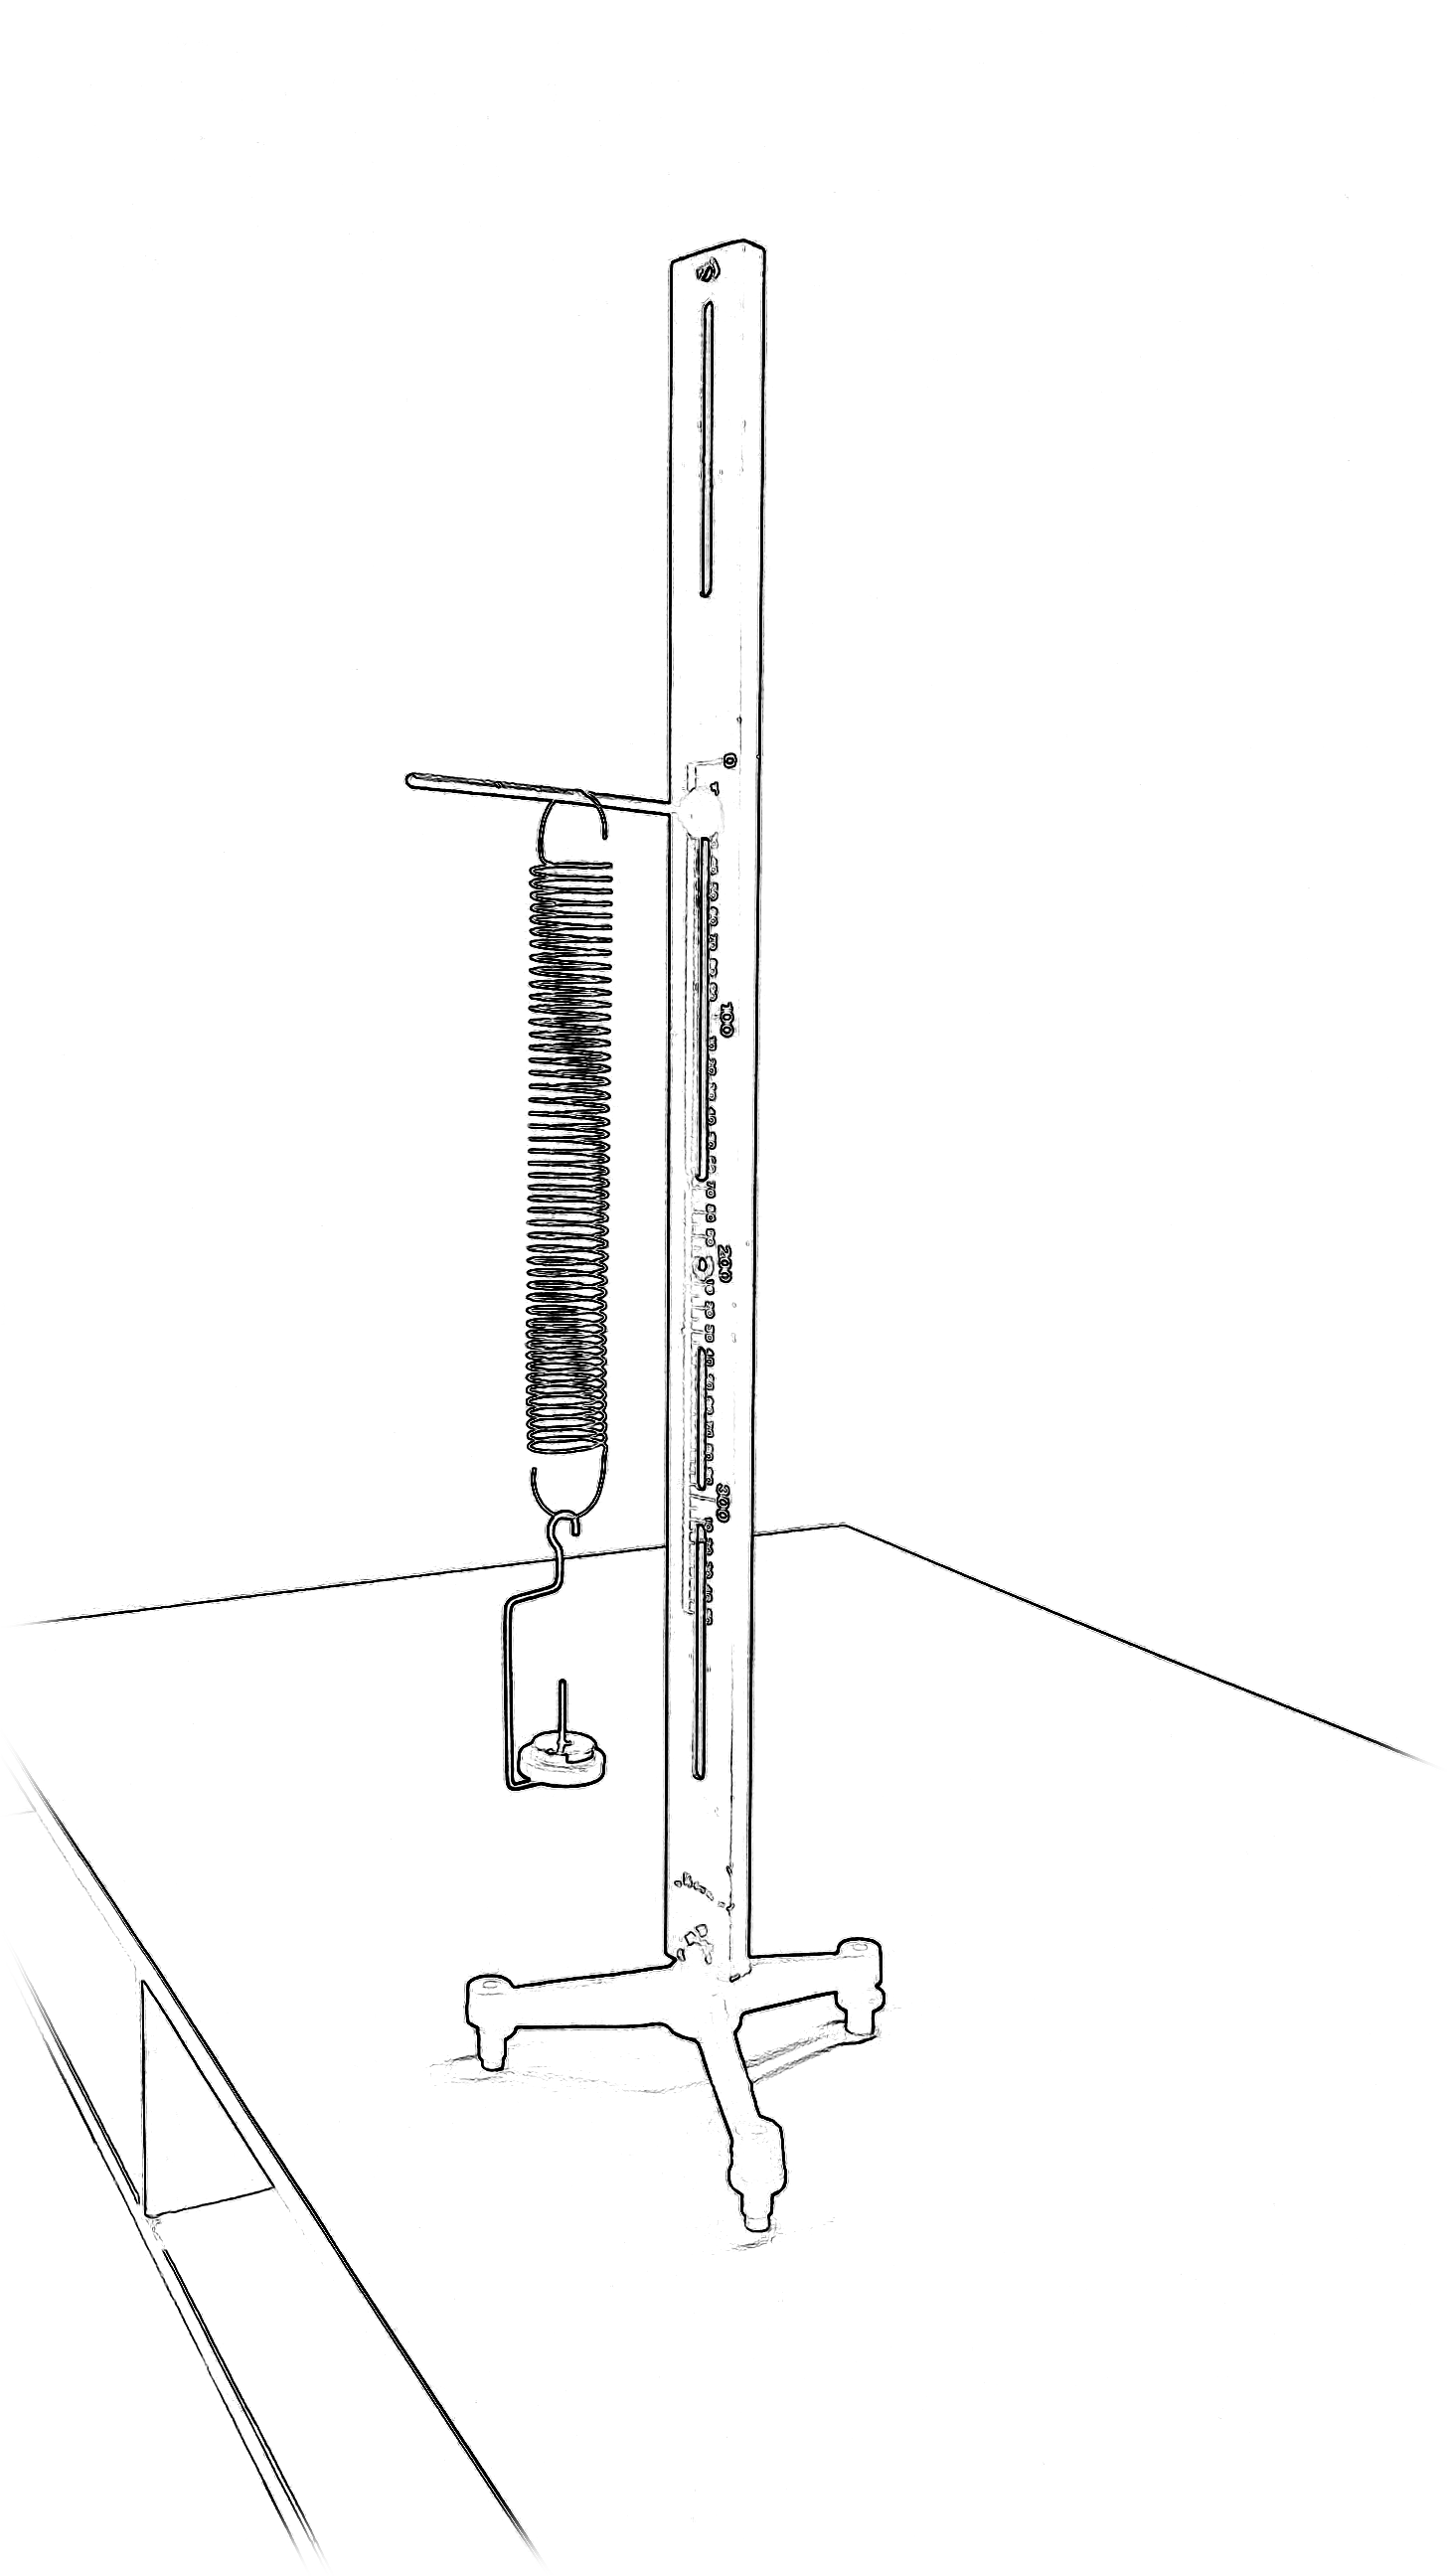
\includegraphics[width=\textwidth]{Ilustrations/Hooke.png}
\caption{Aparato para a verificação da distensão de um mola em função da massa por ela suportada.\label{Fig:IlustracaoLeiDeHooke}}
\end{marginfigure}

\begin{marginfigure}
\centering
\begin{tikzpicture}[>=Stealth]

    \draw[dashed, ->] (0,-1.5) -- (0,1.5) node[below left]{$y$};

	\draw[fill] (0,0) circle[radius = 0.1];
	\draw[->] (0,0) -- node[right]{$\vec{F}_e$}(0,1);
	\draw[->] (0,0) -- node[right]{$\vec{P}$}(0,-1);
	
\end{tikzpicture}
\caption{Diagrama de corpo livre para o corpo sustentado pela mola quando em equilíbrio.}
\label{DiagramaCorpoLivre}
\end{marginfigure}

Para uma mola, se realizarmos o mesmo procedimento, verificamos que ele sofre uma distensão \emph{distensão} gradual à medida que sustenta um peso maior. Fazendo um \emph{diagrama de corpo livre} (Figura~\ref{DiagramaCorpoLivre}), sabendo ainda que a aceleração do sistema é zero em uma condição de equilíbrio, concluímos que a força exercida pela mola sobre a caixa é igual em módulo e tem direção contrária à força peso da caixa (juntamente com sua carga):
\begin{align}
    F_{R, y} &= ma_y \\
    F_{e,y} + P_y &= 0 \\
    F_e - P &= 0 \\
	F_e &= P.
\end{align}

Verificando ainda a distensão $D$ da mola, podemos relacionar uma maior distensão a uma carga maior na caixa, isto é, quanto maior a força peso dos objetos pendurados na mola, maior a distensão. Experimentalmente, verifica-se que a relação entre o peso aplicado à mola e sua distensão são \emph{diretamente proporcionais}:
\begin{equation}
	D \propto P.
\end{equation}

Podemos então escrever para o módulo da \textbf{força elástica} $F_e$
\begin{equation}
	F_e \propto D.
\end{equation}
%
Podemos escrever a relação acima como uma igualdade introduzindo uma constante de proporcionalidade $k$:
\begin{equation}\label{Eq:LeiDeHookeEmModulo}
	F_e = k D.
\end{equation}

O resultado acima é conhecido como \emph{Lei de Hooke}, em homenagem ao físico inglês Robert Hooke, que o verificou em 1660. Tal relação, no entanto, só é válida para um intervalo de distensões da mola. As distensões dentro deste limite são denominadas \emph{elásticas} e não deformam a mola permanentemente, caso contrário ao das distensões \emph{plásticas}. Apesar de a validade da Lei de Hooke ser limitada, ela é o modelo mais comum ao se analisar a resposta de um meio a uma deformação e pode ser utilizada como uma primeira aproximação mesmo para casos mais complexos.

Outro ponto que devemos considerar é o que acontece quando \emph{comprimimos} a mola. Se exercermos uma força conhecida, é possível verificar experimentalmente que a distensão sofrida pela mola segue a mesma relação linear dada pela Equação~\eqref{Eq:LeiDeHookeEmModulo}, com a mesma constante de proporcionalidade. Se considerarmos que a mola é helicoidal ---~como a mostrada na Figura~\ref{Fig:IlustracaoLeiDeHooke}~---, sendo que executamos deslocamentos somente na direção do próprio eixo da mola, podemos escrever uma relação vetorial que denota a direção e o sentido da força tanto para o caso da distensão, quanto para o caso da compressão da mola:
\begin{equation}
    \vec{F}_e = - k \vec{\Delta r}.
\end{equation}
%
Note que o sinal negativo implica em uma força que tem sempre o sentido oposto àquele que submetemos a mola, ou seja, a mola sempre exerce uma força no sentido de \emph{restaurar seu comprimento original}.\footnote{ Devido a isso, a força elástica denominada como uma \emph{força restauradora}.} Se optarmos por usar um sistema de referência, podemos colocar um dos eixos na direção do eixo da própria mola. Se nomearmos tal eixo como $x$, temos que
\begin{align}
    F_{e,x} &= -k \Delta x \\
    F_e &= -k \Delta x, \label{Eq:LeiDeHookeComoTodosConhecemos}
\end{align}
%
onde usamos o fato de que o vetor $\vec{F}_{e}$ aponta diretamente na direção de $x$, o que implica em $F_{e,x} \equiv F_e$ e $\Delta x$ representa a projeção do vetor $\Delta \vec{r}$ na direção do eixo $x$.\footnote{Note que se $\Delta r$ aponta na direção do eixo $x$, então $\Delta r = |\Delta \vec{r}| \equiv \Delta x$, mas a notação que todo mundo utiliza é a da Equação~\eqref{Eq:LeiDeHookeComoTodosConhecemos}. Só estou mostrando de onde essa forma vem.}

%%%%%%%%%%%%%%%%%%%%%%%%%%%%%%%%%%%%%%%%%%%%%
%\subsection{Se necessário, usar subsections}
%%%%%%%%%%%%%%%%%%%%%%%%%%%%%%%%%%%%%%%%%%%%%

%%%%%%%%%%%%%%%%%%%%%%%%%%%%%%%%%%%%%%%%%%%%%%%%%%%%%%%%%%%%%%%%%%%%%%%%%%%%%%%%%%%%%%%%
\section{Experimento: Determinação da distensão de uma mola em função da massa suspensa}
%%%%%%%%%%%%%%%%%%%%%%%%%%%%%%%%%%%%%%%%%%%%%%%%%%%%%%%%%%%%%%%%%%%%%%%%%%%%%%%%%%%%%%%%

Visando verificar a Lei de Hooke, vamos determinar a distensão de uma mola helicoidal posicionada verticalmente em função da massa de um conjunto de anilhas sustentada pela mola e em repouso. As anilhas serão ligadas à mola através de um gancho, permitindo que as depositemos uma a uma, verificando a distensão obtida para cada valor de massa suspensa. Note que devemos tomar o cuidado de verificar a distensão da mola sempre quando as anilhas suspensas se encontram em equilíbrio.

%%%%%%%%%%%%%%%%%%%%%%
\subsection{Objetivos}
%%%%%%%%%%%%%%%%%%%%%%

\begin{itemize}
     \item Verificar a lineariedade da distensão de uma mola em resposta à força peso dos objetos pendurados nela.
	 \item Relacionar as variáveis da Lei de Hooke às da equação da reta $y = A + Bx$.
     \item Calcular a constante $k$ da mola;
     \item Elaborar um gráfico $\Delta x \times P$ dos pontos experimentais e adicionar a ele a reta calculada através da regressão linear;
\end{itemize}

%%%%%%%%%%%%%%%%%%%%%%%%%%%%%%%%%%%%%%%%%%%%%%%%%%%%%%%%%%%%%%%%%%%%%%%%%%%%%%%
\section{Material Necessário}
%%%%%%%%%%%%%%%%%%%%%%%%%%%%%%%%%%%%%%%%%%%%%%%%%%%%%%%%%%%%%%%%%%%%%%%%%%%%%%%

\begin{itemize}
	\item Suporte vertical graduado com base e travessa horizontal;
	\item Molas diversas;
	\item Gancho e anilhas;
	\item Balança;
	\item Régua.
\end{itemize}

%%%%%%%%%%%%%%%%%%%%%%%%%%%%%%%%%%%%%%%%%%%%%%%%%%%%%%%%%%%%%%%%%%%%%%%%%%%%%%%
\section{Procedimento Experimental}
%%%%%%%%%%%%%%%%%%%%%%%%%%%%%%%%%%%%%%%%%%%%%%%%%%%%%%%%%%%%%%%%%%%%%%%%%%%%%%%

\begin{enumerate}
	\item Utilize o suporte para fixar a mola por uma extremidade e prenda o gancho à outra extremidade.
	\item Marque um ponto de referência e meça sua distância a partir da mesa utilizando a régua. Anote o valor na tabela.
	\item Adicione uma anilha e verifique a nova distância do ponto de referência até a mesa. Anote o valor na tabela.
	\item Repita este procedimento adicionando anilhas uma a uma. Procure conseguir o máximo número de pontos experimentais possível, porém sem submeter a mola a deformações irreversíveis.
\end{enumerate}

%%%%%%%%%%%%%%%%%%%%%%%%%%%%%%%%%%%%%%%%%%%%%%%%%%%%%%%%%%%%%%%%%%%%%%%%%%%%%%%
%%%%%%%%%%%%%%%%%%%%%%%%%%%%%%%%%%%%%%%%%%%%%%%%%%%%%%%%%%%%%%%%%%%%%%%%%%%%%%%
%%%%%%%%%%%%%%%%%%%%%%%%%%%%%%%%%%%%%%%%%%%%%%%%%%%%%%%%%%%%%%%%%%%%%%%%%%%%%%%
%%%%%%%%%%%%%%%%%%%%%%%%%%%%%%%%%%%%%%%%%%%%%%%%%%%%%%%%%%%%%%%%%%%%%%%%%%%%%%%
\cleardoublepage

\noindent{}{\huge\textit{Lei de Hooke}}

\vspace{15mm}

\begin{fullwidth}
\noindent{}\makebox[0.6\linewidth]{Turma:\enspace\hrulefill}\makebox[0.4\textwidth]{  Data:\enspace\hrulefill}
\vspace{5mm}

\noindent{}\makebox[0.6\linewidth]{Aluno(a):\enspace\hrulefill}\makebox[0.4\textwidth]{  Matrícula:\enspace\hrulefill}

\noindent{}\makebox[0.6\linewidth]{Aluno(a):\enspace\hrulefill}\makebox[0.4\textwidth]{  Matrícula:\enspace\hrulefill}

\noindent{}\makebox[0.6\linewidth]{Aluno(a):\enspace\hrulefill}\makebox[0.4\textwidth]{  Matrícula:\enspace\hrulefill}

\noindent{}\makebox[0.6\linewidth]{Aluno(a):\enspace\hrulefill}\makebox[0.4\textwidth]{  Matrícula:\enspace\hrulefill}

\noindent{}\makebox[0.6\linewidth]{Aluno(a):\enspace\hrulefill}\makebox[0.4\textwidth]{  Matrícula:\enspace\hrulefill}
\end{fullwidth}

\vspace{5mm}

%%%%%%%%%%%%%%%%%%%%%%%%%%%%%%%%%%%%%%%%%%%%%%%%%%%%%%%%%%%%%%%%%%%%%%%%%%%%%%%
\section{Questionário}
%%%%%%%%%%%%%%%%%%%%%%%%%%%%%%%%%%%%%%%%%%%%%%%%%%%%%%%%%%%%%%%%%%%%%%%%%%%%%%%

\begin{question}[type={exam}]{1}
Apresente os resultados de maneira clara e organizada. Mostre os cálculos requisitados de maneira clara e sucinta, evidenciando o raciocínio desenvolvido.
\end{question}

\begin{question}[type={exam}]{2}
Preencha as colunas de dados experimentais das tabelas com o número adequado de algarismos significativos e unidades.
\end{question}

\begin{question}[type={exam}]{1} 
Calcule a constante $k$ da mola, para cada conjunto de valores de peso e distensão.
\end{question}

\begin{question}[type={exam}]{1} 
Relacione as variáveis da Lei de Hooke àquelas da equação da reta e inteprete o significado das constante $A$ e $B$.
\end{question}

\begin{question}[type={exam}]{2} 
Determine a constante da mola através da regressão linear.
\end{question}

\begin{question}[type={exam}]{2} 
Elabore um gráfico dos pontos experimentais ($\Delta x \times P$) e adicione a ele a reta calculada através da regressão linear.
\end{question}

\begin{question}[type={exam}]{1} 
Determine o valor de $r^2$. O valor encontrado demonstra compatibilidade entre os dados experimentais e a hipótese de dependência linear da distensão com a força aplicada à mola?
\end{question}
\vfill

%%%%%%%%%%%%%%%%%%%%%%%%%%%%%%%%%%%%%%%%%%%%%%%%%%%%%%%%%%%%%%%%%%%%%%%%%%%%%%%
\pagebreak
\section{Tabelas}
%%%%%%%%%%%%%%%%%%%%%%%%%%%%%%%%%%%%%%%%%%%%%%%%%%%%%%%%%%%%%%%%%%%%%%%%%%%%%%%

\begin{table}
\centering
\begin{tabular}{lp{25mm}p{25mm}p{25mm}l}
\toprule
	& \multicolumn{3}{l}{\textbf{Dados Experimentais}} \\
	\cmidrule{2-4}
	& $x_0$ & $x_f$ & $m$ & \\
	\cmidrule{2-4}
	& \cellcolor[gray]{0.89} & \cellcolor[gray]{0.92} & \cellcolor[gray]{0.89} \\
	& \cellcolor[gray]{0.95} & \cellcolor[gray]{0.97} & \cellcolor[gray]{0.95} \\
	& \cellcolor[gray]{0.89} & \cellcolor[gray]{0.92} & \cellcolor[gray]{0.89} \\
	& \cellcolor[gray]{0.95} & \cellcolor[gray]{0.97} & \cellcolor[gray]{0.95} \\
	& \cellcolor[gray]{0.89} & \cellcolor[gray]{0.92} & \cellcolor[gray]{0.89} \\
	& \cellcolor[gray]{0.95} & \cellcolor[gray]{0.97} & \cellcolor[gray]{0.95} \\
	& \cellcolor[gray]{0.89} & \cellcolor[gray]{0.92} & \cellcolor[gray]{0.89} \\
	& \cellcolor[gray]{0.95} & \cellcolor[gray]{0.97} & \cellcolor[gray]{0.95} \\
	& \cellcolor[gray]{0.89} & \cellcolor[gray]{0.92} & \cellcolor[gray]{0.89} \\
	& \cellcolor[gray]{0.95} & \cellcolor[gray]{0.97} & \cellcolor[gray]{0.95} \\
	& \cellcolor[gray]{0.89} & \cellcolor[gray]{0.92} & \cellcolor[gray]{0.89} \\
	& \cellcolor[gray]{0.95} & \cellcolor[gray]{0.97} & \cellcolor[gray]{0.95} \\
	\cmidrule{2-4}
\\
	& \multicolumn{3}{l}{\textbf{Valores calculados}} \\
	\cmidrule{2-4}
	& $|\Delta x|$ & $P$ & $P/\Delta x$ \\
	\cmidrule{2-4}
	& \cellcolor[gray]{0.89} & \cellcolor[gray]{0.92} & \cellcolor[gray]{0.89} \\
	& \cellcolor[gray]{0.95} & \cellcolor[gray]{0.97} & \cellcolor[gray]{0.95} \\
	& \cellcolor[gray]{0.89} & \cellcolor[gray]{0.92} & \cellcolor[gray]{0.89} \\
	& \cellcolor[gray]{0.95} & \cellcolor[gray]{0.97} & \cellcolor[gray]{0.95} \\
	& \cellcolor[gray]{0.89} & \cellcolor[gray]{0.92} & \cellcolor[gray]{0.89} \\
	& \cellcolor[gray]{0.95} & \cellcolor[gray]{0.97} & \cellcolor[gray]{0.95} \\
	& \cellcolor[gray]{0.89} & \cellcolor[gray]{0.92} & \cellcolor[gray]{0.89} \\
	& \cellcolor[gray]{0.95} & \cellcolor[gray]{0.97} & \cellcolor[gray]{0.95} \\
	& \cellcolor[gray]{0.89} & \cellcolor[gray]{0.92} & \cellcolor[gray]{0.89} \\
	& \cellcolor[gray]{0.95} & \cellcolor[gray]{0.97} & \cellcolor[gray]{0.95} \\
	& \cellcolor[gray]{0.89} & \cellcolor[gray]{0.92} & \cellcolor[gray]{0.89} \\
	& \cellcolor[gray]{0.95} & \cellcolor[gray]{0.97} & \cellcolor[gray]{0.95} \\
	\cmidrule{2-4}
\bottomrule
\end{tabular}
\caption{Valores de posição em função da massa pendurada na mola.}
\label{Dados}
\end{table}

%%%%%%%%%%%%%%%%%%%%%%%%%%%%%%%%%%%%%%%%%%%%%%%%%%%%%%%%%%%%%%%%%%%%%%%%%%%%%%%%
\chapter{Leis de Newton}
\label{Chap:ExpLeisDeNewton}
%%%%%%%%%%%%%%%%%%%%%%%%%%%%%%%%%%%%%%%%%%%%%%%%%%%%%%%%%%%%%%%%%%%%%%%%%%%%%%%

\begin{fullwidth}\it
	Realizaremos um experimento no qual dois corpos estão ligados por um fio, sendo que um deles pode se deslocar livremente no eixo vertical, enquanto o outro se desloca no eixo horizontal. Através desse aparato, poderemos calcular a aceleração através das Leis de Newton --- assumindo que podemos determinar as forças que atuam sobre o sistema, exceto pelas forças de atrito e arrasto, que devem ser desprezíveis ---. Além disso, seremos capazes de calcular a aceleração através de informações cinemáticas (distância percorrida e tempo correspondente), permitindo uma comparação entre os valores obtidos. Utilizaremos os conceitos de medidas, algarismos significativos, gráficos, erros de escala e propagados, regressão linear, e linearização.
\end{fullwidth}

%%%%%%%%%%%%%%%%%%%%%%%%%%%%%%%%%%%%%%%%%%%%%%%%%%%%%%%%%%%%%%%%%%%%%%%%%%%%%%%
\section{Leis de Newton}
%%%%%%%%%%%%%%%%%%%%%%%%%%%%%%%%%%%%%%%%%%%%%%%%%%%%%%%%%%%%%%%%%%%%%%%%%%%%%%%

Ao estudar o movimento dos corpos, verificamos que são necessárias três grandezas para descrever o movimento: a \emph{posição}, a \emph{velocidade} e a \emph{aceleração}. Além disso, sabemos que estas três grandezas estão relacionadas através de
\begin{align}
	\vec{v} &= \frac{d\vec{r}}{dt} \\
	\vec{a} &= \frac{d\vec{v}}{dt}.
\end{align}

Por outro lado, podemos relacionar o movimento de um corpo às forças que atuam nele através das leis de Newton, que podem ser enunciadas como:
\begin{description}
	\item[1\textordfeminine Lei] Se nenhuma força resultante atua sobre um corpo, sua velocidade não pode mudar, ou seja, o corpo não pode sofrer uma aceleração.
	\item[2\textordfeminine Lei] A força resultante que age sobre um corpo é igual ao produto da massa do corpo pela sua aceleração, isto é,
		\begin{equation}
			\vec{F}_{\textrm{res}} = m\vec{a}.
		\end{equation}
	\item[3\textordfeminine Lei] Quando dois corpos interagem, as forças que cada corpo exerce sobre o outro são sempre iguais em módulo e têm sentidos opostos.
\end{description}
%
Do ponto de vista do estudo do movimento de um corpo submetido a uma ou mais forças, as leis de Newton transferem parte do problema para a determinação de características das forças envolvidas no problema. Devido a isto, é importante conhecermos algumas características das forças mais comuns:
\begin{description}
	\item[Força Peso] A força peso a força gravitacional exercida sobre um corpo próximo à superfície da Terra, sempre em direção ao centro da Terra e com módulo dado por
	\begin{equation}
		P = mg.
	\end{equation}
	A origem de tal expressão é a lei da gravitação universal:
	\begin{equation}
		F_g = G \frac{M_T m}{r_T^2},
	\end{equation}
	onde $G = \np[N\cdot m^2/kg^2]{6,673e-11}$ é a constante da gravitação, $M_T$ é a massa da Terra e $r_T$ é o raio da Terra. Como esse último varia pouco (percentualmente), podemos reescrever a expressão acima como
	\begin{align}
		F_g &= \left[\frac{G M_T}{r_T^2}\right] m \\
			&= mg,
	\end{align}
	onde $g \approx \np[m/s^2]{9,8}$.

\item[Força Normal] A força normal ganha esse nome pois ela é sempre \emph{normal}, ou seja, \emph{perpendicular} à superfície de interação entre dois corpos quaisquer. Quando colocamos um objeto sobre uma mesa, por exemplo, ele estará sujeito à força peso --- devida a atração gravitacional exercida pela Terra sobre o objeto --- e a uma força normal exercida pela mesa sobre o objeto.
	
	Se a mesa for completamente horizontal, a força será dirigida para cima. Sobre o módulo da força, no entanto, não podemos afirmar muita coisa: sabemos que nesse tipo de situação o objeto deve permanecer parado sobre a mesa, de onde concluímos que a normal tem o mesmo módulo que o peso. Se, entretanto, o objeto for uma caixa, poderemos colocar outros objetos dentro dele e assim aumentaremos a força gravitacional exercida sobre o conjunto. Nessa situação observamos que o sistema continua em repouso, de onde concluímos que a força normal aumentou. Podemos afirmar, portanto, que a força normal pode variar em resposta a componente da força peso que é perpendicular à superfície. Por outro lado, se colocarmos uma carga exageradamente grande sobre uma mesa fraca, verificamos que a mesa quebra, portanto concluímos que a força normal deve ter um valor máximo.

	Em situações onde o objeto sobre o qual a força normal age pode ser submetido a acelerações --- dentro de um elevador, por exemplo --- temos uma situação ainda mais complexa. O valor da força normal passa também a variar dependendo do estado de aceleração do sitema elevador-objeto. Percebe-se, portanto, que a determinação exata do valor do módulo da força normal requer uma análise aprofundada da situação em questão.

\item[Tensão] A tensão tem um comportamento bastante similar ao da força normal. Se prendermos um fio ao teto de uma sala e pendurarmos um balde, verificamos que o balde permanecerá em repouso. Portanto, sabemos que a tensão equilibra a força peso. Se enchermos o balde com água, aumentamos a massa do conjunto e, consequentemente, a força peso. Ao fazer isso, no entanto, não notamos nenhum deslocamento do balde (se o fio for inextensível). Se aumentarmos muito a carga do balde, podemos fazer com que o fio atinja e ultrapasse seu valor máximo de tensão, fazendo com que ele se rompa.

	Da mesma forma que com a força normal, se tivermos uma aceleração do sistema, precisaremos leva-lá em consideração ao calcular o valor da tensão. Portanto, também precisamos de uma análise aprofundada da situação em questão.
\end{description}

%%%%%%%%%%%%%%%%%%%%%%%%%%%%%%%%%%%%%%%%%%%%
\section{Máquina de Atwood}
%%%%%%%%%%%%%%%%%%%%%%%%%%%%%%%%%%%%%%%%%%%%

Através dos conceitos expostos acima, podemos fazer uma análise do movimento horizontal de um objeto que é puxado por outro que cai, conforme mostrado na Figura~\ref{FigTrilhoDeAr}. Tal aparato é conhecido como \emph{Máquina de Atwood}. Vamos analisar esse sistema de duas formas distintas, para que possamos comparar os resultados obtidos com cada uma delas.

\begin{figure}
\centering
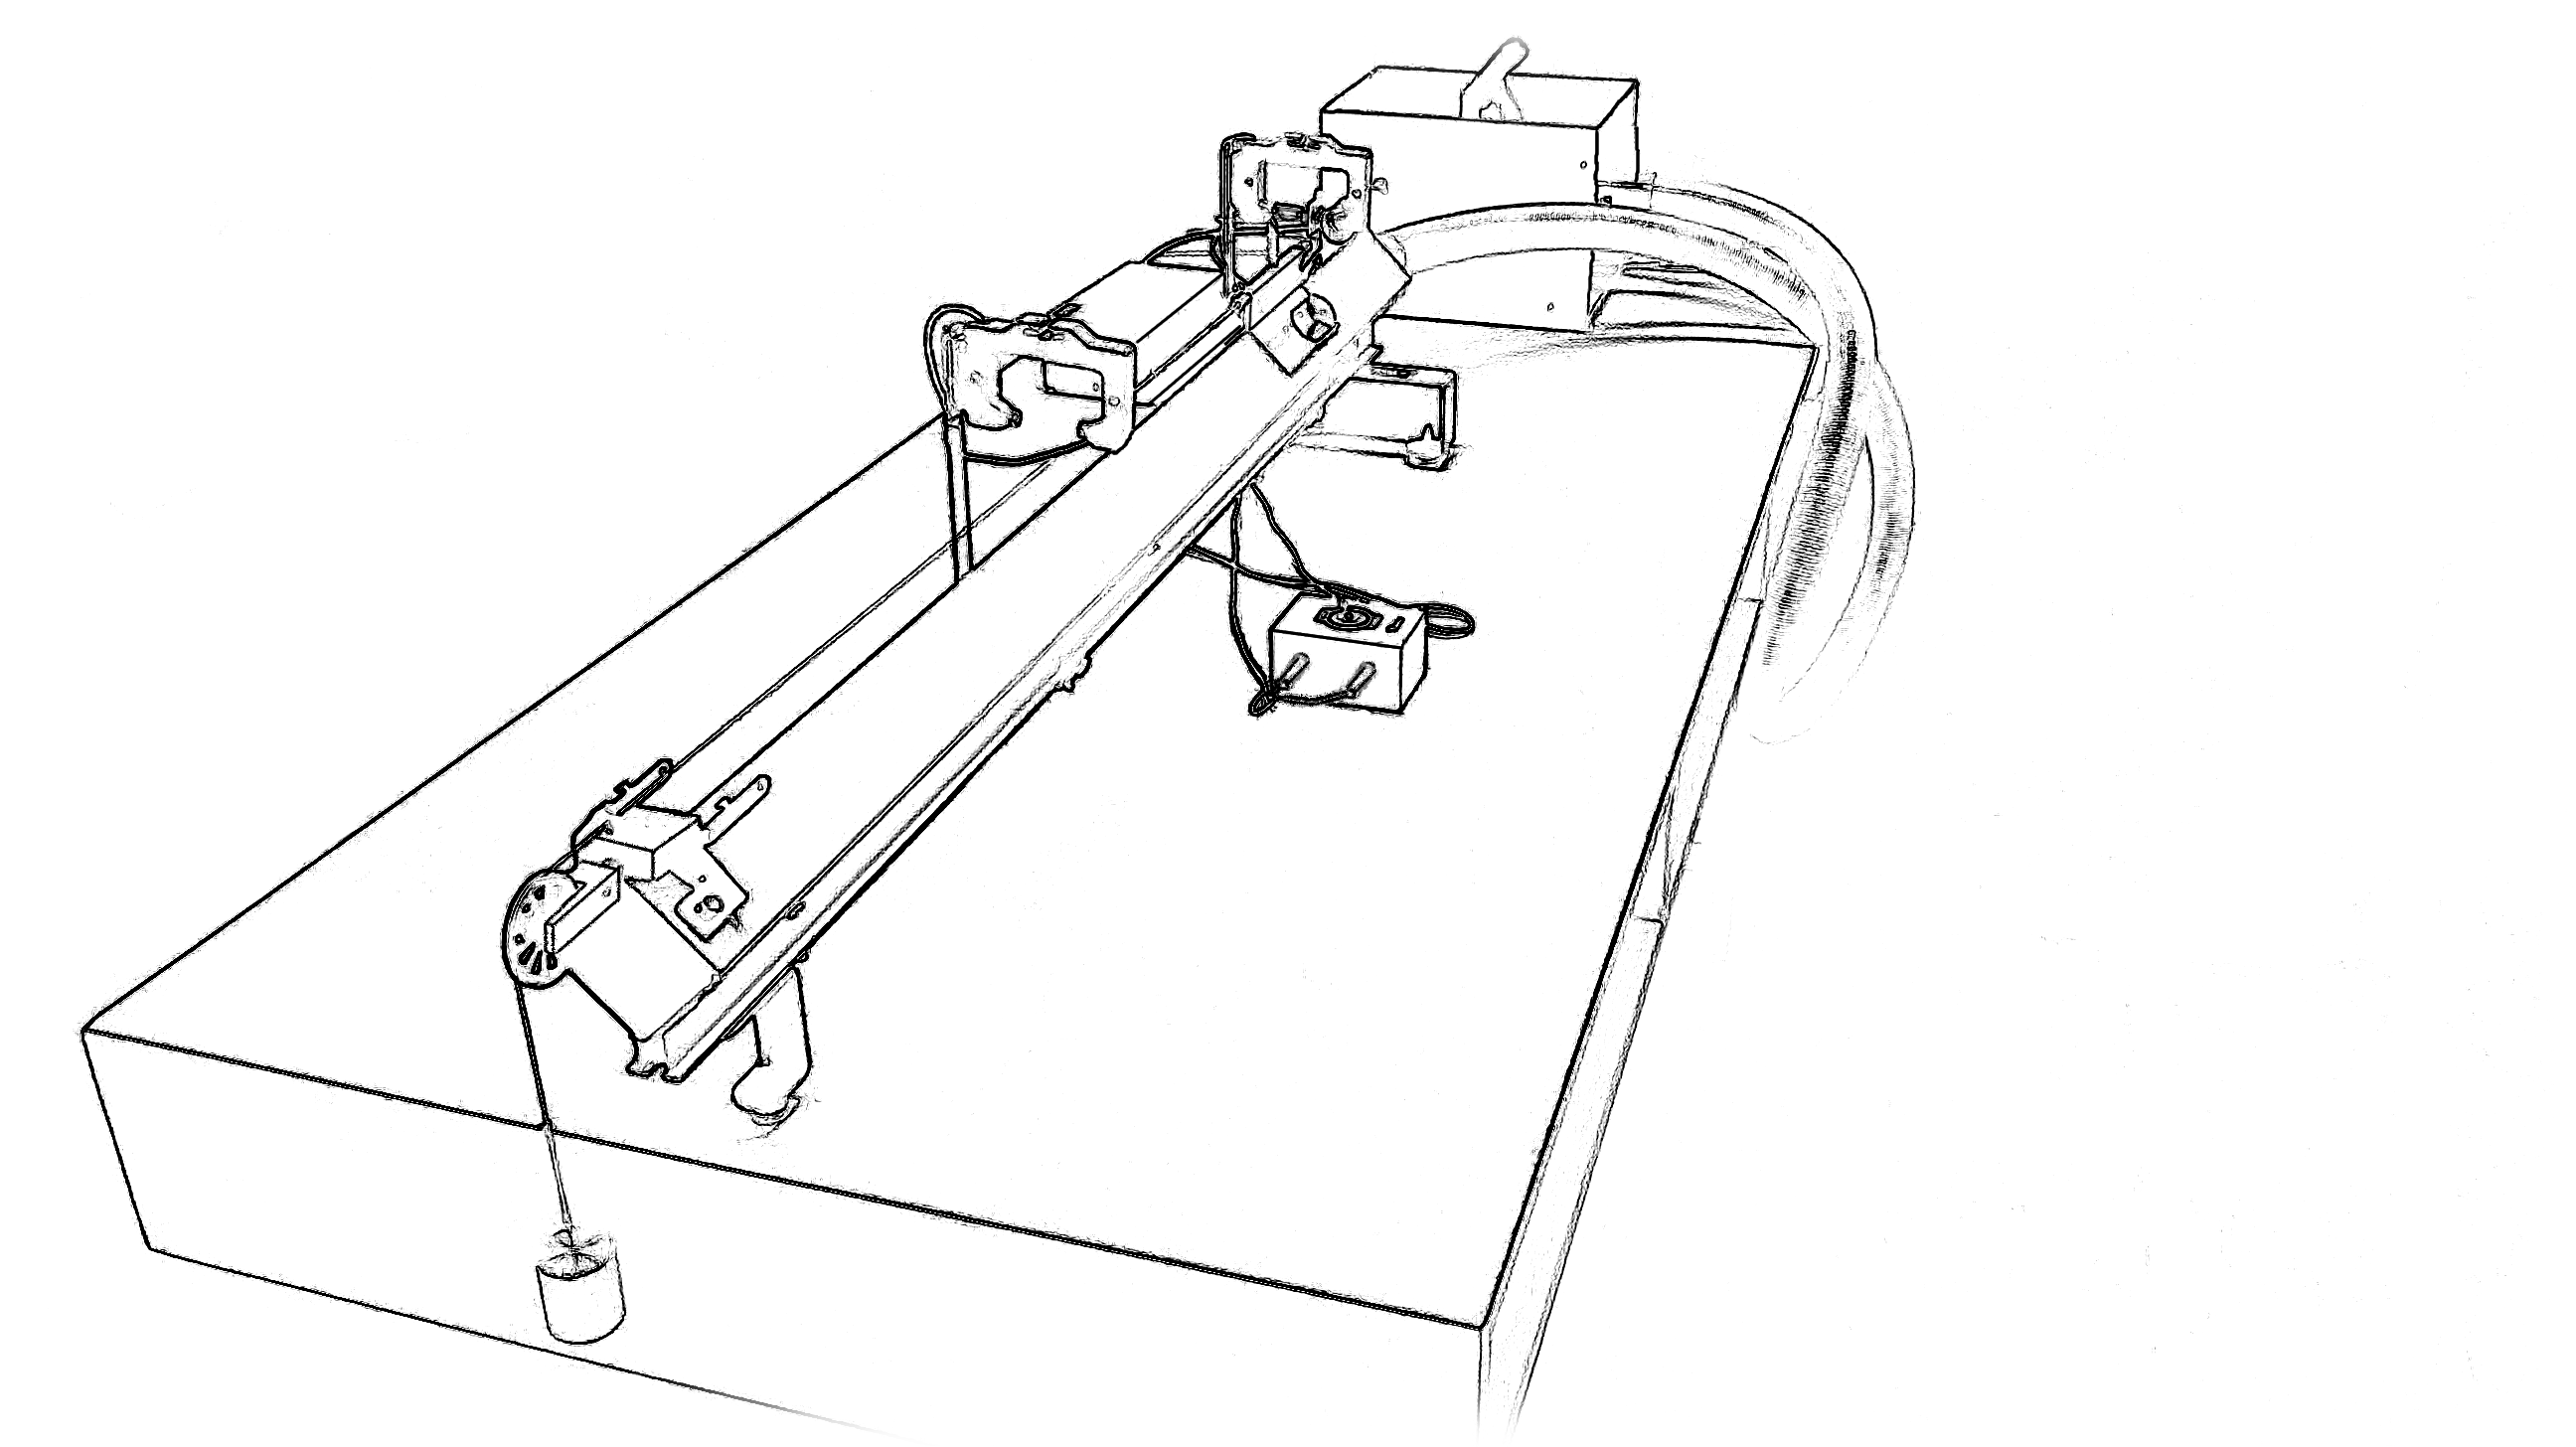
\includegraphics[width=\textwidth]{Ilustrations/TrilhoAr.png}
\caption{Objeto se movendo horizontalmente em um trilho de ar, submetido a uma aceleração devida ao objeto que cai.}
\label{FigTrilhoDeAr}
\end{figure}


%%%%%%%%%%%%%%%%%%%%%%%%%%%%%%%%%%%%%%%%%%%%%%%%%%
\subsection{Análise através das Leis de Newton}
%%%%%%%%%%%%%%%%%%%%%%%%%%%%%%%%%%%%%%%%%%%%%%%%%%

\begin{marginfigure}
\begin{tikzpicture}[>=Stealth]
	% Coordenadas
	\draw[->, dashed, very thin, gray] (0,0.25) -- (5,0.25) node[below]{$x$};
	\draw[->, dashed, very thin, gray] (3.5,-3) -- (3.5,2) node[left]{$y$};

	% mesa
	\draw[gray] (0,0) -- (3,0);
	\draw[gray] (3,0) -- (3,-1);
	
	% roldana	
	\draw[gray] (3.3,0.05) circle[radius = 0.2];
	\draw[gray,fill] (3.3,0.05) circle[radius = 0.05];
	\draw[gray,fill] (2.6,0.1) rectangle (3.3,0);
	\draw[gray,fill] (2.7,0.1) circle[radius = 0.05];
	\draw[gray,fill] (2.9,0.1) circle[radius = 0.05];
	\draw[fill, white] (3.3,0.05) circle[radius = 0.02];
	
	% bloco superior
	\draw (0.5,0) rectangle +(1,0.5);
	\draw[gray] (1.5,0.25) -- (3.3,0.25);
	\draw[->] (1,0) -- +(0,-1) node[left]{$\vec{P}_1$};
	\draw[->] (1.5,0.25) -- +(0.5,0) node[above]{$\vec{T}$};
	\draw[->] (1,0.5) -- +(0,1) node[left]{$\vec{N}$};
	
	% bloco inferior
	\draw[gray] (3.5,0.05) -- +(0,-1);
	\draw (3.3,-0.95) rectangle +(0.4,-0.8);
	\draw[->] (3.5,-0.95) -- +(0,0.5) node[right]{$\vec{T}$};
	\draw[->] (3.5,-1.75) -- +(0,-0.75) node[right]{$\vec{P}_2$};
\end{tikzpicture}
\caption{Desenho esquemático representando os corpos móveis e as forças que neles atuam.}
\end{marginfigure}

Analisando cada um dos objetos separadamente através da segunda lei de Newton:
\begin{itemize}
\item\textbf{Objeto de massa $m_1$:}
\begin{description}
	\item[Eixo $x$:] Como o atrito no trilho de ar é desprezível, temos
		\begin{align}
			F_R &= m_1 a_x \\
			T_1 &= m_1 a_x
		\end{align}
	\item[Eixo $y$:] Sabemos que a aceleração neste eixo é zero, logo
		\begin{align}
			F_R &= 0 \\
			N - P_1 &= 0.
		\end{align}
\noindent{}De onde podemos escrever
		\begin{align}
			N &= P_1 \\
			  &= m_1 g.
		\end{align}
\end{description}

\begin{marginfigure}
\begin{tikzpicture}[>=Stealth]
	% Coordenadas objeto esquerdo
	\draw[->, very thin, dashed, gray] (-1,0) -- (1,0) node[below]{$x$};
	\draw[->, very thin, dashed, gray] (0,-1.5) -- (0,1.5) node[left]{$y$};
	
	% Objeto esquerdo
	\draw[fill] (0,0) circle[radius = 0.1];
	
	% Vetores
	\draw[->] (0,0) -- +(0.5,0) node[below]{$\vec{T}$};
	\draw[->] (0,0) -- +(0,1) node[left]{$\vec{N}$};
	\draw[->] (0,0) -- +(0,-1) node[left]{$\vec{P}_1$};
	
	% Coordenadas objeto direito
	\draw[->, very thin, dashed, gray] (1.75,0) -- +(1.5,0) node[below]{$x$};
	\draw[<-, very thin, dashed, gray] (2.5,0) +(0,1.5) node[left]{$y$} -- +(0,-1.5);
	
	% Objeto direito
	\draw[fill] (2.5,0) circle[radius=0.1];
	
	% Vetores
	\draw[->] (2.5,0) -- +(0,-0.75) node[right]{$\vec{P}_2$};
	\draw[->] (2.5,0) -- +(0,0.5) node[right]{$\vec{T}$};
\end{tikzpicture}
\caption{Diagramas de corpo livre para ambos os corpos.}
\end{marginfigure}

\item\textbf{Objeto de massa $m_2$:}
\begin{description}
	\item[Eixo $x$:] Nenhuma força atua no eixo $x$.
	\item[Eixo $y$:] Como atuam somente o peso e a tensão neste eixo, temos
		\begin{align}
			F_R &= m_2 a_y \\
			T_2 - P_2 &= m_2 a_y.
		\end{align}
\end{description}
\end{itemize}

Como ambos os objetos estão ligados por uma corda --- que consideraremos inextensível e de massa desprezível ---, sabemos que as acelerações dos blocos devem ter o mesmo módulo. Consequentemente,
	\begin{equation}
		a_x = -a_y.
	\end{equation}
%
Vamos também considerar que a roldana tem massa desprezível. Dessa forma, é possível mostrar usando uma versão da segunda lei de Newton para as rotações que o módulo das tensões $T_1$ e $T_2$ deve ser o mesmo. Podemos então resumir a análise desse sistema através do seguinte conjunto de equações:
\begin{align}
	T &= m_1 a\\
	T-m_2g &= -m_2 a
\end{align}

Resolvendo este sistema, concluímos que
\begin{align}
	a &= \frac{m_2}{m_1 + m_2} g \label{EqAceleracao}\\
	T &= \frac{m_1m_2}{m_1+m_2}g.
\end{align}

Portanto, conhecendo o valor das massas dos dois objetos, temos condições de calcular a aceleração do sistema.

%%%%%%%%%%%%%%%%%%%%%%%%%%%%%%%%%%%%%%%%%%%%%%%%%%%%%%%%%%%
\subsection{Análise através das equações da cinemática.}
%%%%%%%%%%%%%%%%%%%%%%%%%%%%%%%%%%%%%%%%%%%%%%%%%%%%%%%%%%%

Uma outra forma de análise do sistema é através das equações da cinemática. Se formos capazes de medir a distância percorrida por qualquer um dos blocos e pudermos cronometrar o tempo necessário para realizar tal deslocamento, podemos extrair a aceleração dos dados utilizando a fórmula para o deslocamento de um objeto submetido a uma aceleração constante, isto é,
	\begin{equation}
		\Delta x = v_0 t + \frac{1}{2} at^2
	\end{equation}

Como podemos iniciar a cronometragem assim que o objeto começa a se mover, podemos eliminar a velocidade inicial $v_0$. Assim
\begin{equation}
	\Delta x = \frac{1}{2} at^2.
\end{equation}

Podemos calcular a aceleração a partir de um valor qualquer de deslocamento e do tempo correspondente. No entanto, o mais adequado é realizar uma série de medidas e utilizar o método dos mínimos quadrados para o conjunto de dados linearizado. Fazendo uma linearização, tratando $\Delta x$ como variável independente, obtemos a seguinte relação entre a equação da reta e a equação acima:
\begin{align}
	y &= t^2 \\
	A &= 0 \\
	B &= 2/a \\
	x &= \Delta x.
\end{align}
%
Podemos então calcular o coeficiente angular através de uma regressão linear dos dados obtidos para o deslocamento e para o tempo ao quadrado e obter um valor de aceleração independente daquele calculado através das leis de Newton. Isso possibilitará que comparemos os valores obtidos, testando assim a validade de tais leis.

%%%%%%%%%%%%%%%%%%%%%%%%%%%%%%%%%%%%%%%%%%%%%%%%%%%%%%%%%%%%%%%%%%%%%%%%%%%%%%%
\section{Experimento}
%%%%%%%%%%%%%%%%%%%%%%%%%%%%%%%%%%%%%%%%%%%%%%%%%%%%%%%%%%%%%%%%%%%%%%%%%%%%%%%

%%%%%%%%%%%%%%%%%%%%%%
\subsection{Objetivos}
%%%%%%%%%%%%%%%%%%%%%%

\begin{itemize}
     \item Verificar a validade das Leis de Newton;
	 \item Linearizar o conjunto de dados obtidos e obter os valores de $A$ e $B$ da equação da reta correspondente;
	 \item Relacionar as variáveis cinemáticas às constantes da equação da reta;
     \item Calcular a aceleração do sistema através do valor do coeficiente angular ($B$) da reta;
     \item Elaborar um gráfico $\Delta x \times t$ dos pontos experimentais;
	 \item Elaborar um gráfico $\Delta x \times t^2$ dos pontos experimentais e adicionar a ele a reta obtida através da regressão linear.
\end{itemize}

%%%%%%%%%%%%%%%%%%%%%%%%%%%%%%%%%%%%%%%%%%%%%%%%%%%%%%%%%%%%%%%%%%%%%%%%%%%%%%%
\section{Material Necessário}
%%%%%%%%%%%%%%%%%%%%%%%%%%%%%%%%%%%%%%%%%%%%%%%%%%%%%%%%%%%%%%%%%%%%%%%%%%%%%%%

\begin{itemize}
	\item Conjunto de trilho de ar com sensores e cronômetro;
	\item Gancho e anilhas;
	\item Balança;
\end{itemize}

%%%%%%%%%%%%%%%%%%%%%%%%%%%%%%%%%%%%%%%%%%%%%%%%%%%%%%%%%%%%%%%%%%%%%%%%%%%%%%%
\section{Procedimento Experimental}
%%%%%%%%%%%%%%%%%%%%%%%%%%%%%%%%%%%%%%%%%%%%%%%%%%%%%%%%%%%%%%%%%%%%%%%%%%%%%%%

\begin{enumerate}
	\item Afira as massas do ``carrinho'' que se desloca sobre o trilho de ar e do conjunto formado pelo gancho e pelas anilhas. Anote os valores obtidos na Tabela~\ref{TabelaDadosLeisDeNewton}.
	\item Posicione o primeiro sensor imediatamente após a região do carrinho que ativa o sensor, de forma a garantir que a velocidade inicial seja nula;
	\item Posicione o segundo sensor a uma distância de cerca de \np[cm]{8,00} após o primeiro.
	\item Libere o carrinho e anote os valores obtidos de tempo e de distância percorrida na Tabela~\ref{TabelaDadosLeisDeNewton}.
	\item Desloque o segundo sensor distanciando-o mais \np[cm]{4,00} do primeiro.
	\item Libere o carrinho novamente e anote os novos valores de tempo e de distância percorrida na Tabela~\ref{TabelaDadosLeisDeNewton}.
	\item Repita os dois itens acima com tantos dados quanto possível. Observe que conforme o conjunto de anilhas desce, ele eventualmente colide com o chão. \textbf{A colisão com o chão só pode acontecer após o carrinho ter passado pelo segundo sensor.} Portanto, o valor máximo de distância entre os sensores estará limitado por esse fator. 
\end{enumerate}

%%%%%%%%%%%%%%%%%%%%%%%%%%%%%%%%%%%%%%%%%%%%%%%%%%%%%%%%%%%%%%%%%%%%%%%%%%%%%%%
%%%%%%%%%%%%%%%%%%%%%%%%%%%%%%%%%%%%%%%%%%%%%%%%%%%%%%%%%%%%%%%%%%%%%%%%%%%%%%%
%%%%%%%%%%%%%%%%%%%%%%%%%%%%%%%%%%%%%%%%%%%%%%%%%%%%%%%%%%%%%%%%%%%%%%%%%%%%%%%
%%%%%%%%%%%%%%%%%%%%%%%%%%%%%%%%%%%%%%%%%%%%%%%%%%%%%%%%%%%%%%%%%%%%%%%%%%%%%%%
\cleardoublepage

\noindent{}{\huge\textit{Leis de Newton}}

\vspace{15mm}

\begin{fullwidth}
\noindent{}\makebox[0.6\linewidth]{Turma:\enspace\hrulefill}\makebox[0.4\textwidth]{  Data:\enspace\hrulefill}
\vspace{5mm}

\noindent{}\makebox[0.6\linewidth]{Aluno(a):\enspace\hrulefill}\makebox[0.4\textwidth]{  Matrícula:\enspace\hrulefill}

\noindent{}\makebox[0.6\linewidth]{Aluno(a):\enspace\hrulefill}\makebox[0.4\textwidth]{  Matrícula:\enspace\hrulefill}

\noindent{}\makebox[0.6\linewidth]{Aluno(a):\enspace\hrulefill}\makebox[0.4\textwidth]{  Matrícula:\enspace\hrulefill}

\noindent{}\makebox[0.6\linewidth]{Aluno(a):\enspace\hrulefill}\makebox[0.4\textwidth]{  Matrícula:\enspace\hrulefill}

\noindent{}\makebox[0.6\linewidth]{Aluno(a):\enspace\hrulefill}\makebox[0.4\textwidth]{  Matrícula:\enspace\hrulefill}
\end{fullwidth}

\vspace{5mm}

%%%%%%%%%%%%%%%%%%%%%%%%%%%%%%%%%%%%%%%%%%%%%%%%%%%%%%%%%%%%%%%%%%%%%%%%%%%%%%%
\section{Questionário}
%%%%%%%%%%%%%%%%%%%%%%%%%%%%%%%%%%%%%%%%%%%%%%%%%%%%%%%%%%%%%%%%%%%%%%%%%%%%%%%
\emph{Nas questões seguintes, apresente os cálculos requisitados de maneira clara e sucinta, para que o professor possa acompanhar o raciocínio desenvolvido.}
\vspace{5mm}

\begin{question}[type={exam}]{2}
Preencha as tabelas com unidades e número de algarismos significativos adequados. Calcule também o erro propagado para os valores de $t^2$.
\end{question}

\begin{question}[type={exam}]{2.5}
Elabore um gráfico $ t \times \Delta x$ dos pontos experimentais e um gráfico de $t^2 \times \Delta x$.
\end{question}

\begin{question}[type={exam}]{2}
Através dos gráficos elaborados no item anterior, podemos verificar qual dos dois conjuntos de dados segue uma tendência linear. Para o conjunto de dados linear, obtenha os valores de $A$, $B$ e $r^2$ da melhor reta correspondente (a reta da regressão linear). Adicione essa reta ao gráfico e coloque a equação da reta, juntamente com o coeficiente $r^2$ na legenda.
\end{question}

\begin{question}[type={exam}]{1.5}
Relacione as variáveis cinemáticas às constantes da equação da reta. Calcule através do coeficiente angular ($B$) qual é a aceleração do sistema.
\end{question}

\begin{question}[type={exam}]{1}
Compare o valor o valor obtido para a aceleração com o valor dado pelas leis de Newton. Utilize a fórmula
\begin{equation}
	E_\% = \left|\frac{x - x_{\textrm{Ref}}}{x_{\textrm{Ref}}}\right| \times 100
\end{equation}
%
--- onde $x_{\textrm{Ref}}$ é um valor de referência e $x$ é um valor que queremos comparar com o valor de referência --- e calcule o erro percentual entre o valor obtido pela regressão linear dos dados cinemáticos e o valor obtido através das Leis de Newton. \emph{(No nosso caso caso, $x_{\textrm{Ref}}$ é o valor obtido para a aceleração através das Leis de Newton e $x$ é o valor obtido através do coeficiente $B$ da regressão linear.)}
\end{question}

\begin{question}[type={exam}]{1}
Inverta a Equação~\eqref{EqAceleracao} e isole a gravidade. Use o valor da aceleração obtido através dos dados cinemáticos e calcule o valor de $g$. Utilize a fórmula para o erro percentual e calcule $E_\%$ com relação ao valor $g=\np[m/s^2]{9,8}$.
\end{question}

\vfill
%%%%%%%%%%%%%%%%%%%%%%%%%%%%%%%%%%%%%%%%%%%%%%%%%%%%%%%%%%%%%%%%%%%%%%%%%%%%%%%
\pagebreak
\section{Tabelas}
%%%%%%%%%%%%%%%%%%%%%%%%%%%%%%%%%%%%%%%%%%%%%%%%%%%%%%%%%%%%%%%%%%%%%%%%%%%%%%%

\begin{table}[!ht]
\centering
\begin{tabular}{lp{25mm}p{25mm}p{25mm}l}
\toprule
	& \multicolumn{3}{l}{\textbf{Massas}} \\
	\cmidrule{2-4}
	& \multicolumn{2}{l}{Carrinho \cellcolor[gray]{0.89}} & \cellcolor[gray]{0.92} \\
	& \multicolumn{2}{l}{Gancho e anilhas \cellcolor[gray]{0.95}} & \cellcolor[gray]{0.97}\\
	\cmidrule{2-4}
\\
	&\multicolumn{3}{l}{\textbf{Dados experimentais}} \\
	\cmidrule{2-4}
	& $x_i$ & $x_f$ & $t$ & \\
	\cmidrule{2-4}
	& \cellcolor[gray]{0.89} & \cellcolor[gray]{0.92} & \cellcolor[gray]{0.89} \\
	& \cellcolor[gray]{0.95} & \cellcolor[gray]{0.97} & \cellcolor[gray]{0.95} \\
	& \cellcolor[gray]{0.89} & \cellcolor[gray]{0.92} & \cellcolor[gray]{0.89} \\
	& \cellcolor[gray]{0.95} & \cellcolor[gray]{0.97} & \cellcolor[gray]{0.95} \\
	& \cellcolor[gray]{0.89} & \cellcolor[gray]{0.92} & \cellcolor[gray]{0.89} \\
	& \cellcolor[gray]{0.95} & \cellcolor[gray]{0.97} & \cellcolor[gray]{0.95} \\
	& \cellcolor[gray]{0.89} & \cellcolor[gray]{0.92} & \cellcolor[gray]{0.89} \\
	& \cellcolor[gray]{0.95} & \cellcolor[gray]{0.97} & \cellcolor[gray]{0.95} \\
	& \cellcolor[gray]{0.89} & \cellcolor[gray]{0.92} & \cellcolor[gray]{0.89} \\
	& \cellcolor[gray]{0.95} & \cellcolor[gray]{0.97} & \cellcolor[gray]{0.95} \\
	& \cellcolor[gray]{0.89} & \cellcolor[gray]{0.92} & \cellcolor[gray]{0.89} \\
	& \cellcolor[gray]{0.95} & \cellcolor[gray]{0.97} & \cellcolor[gray]{0.95} \\
	& \cellcolor[gray]{0.89} & \cellcolor[gray]{0.92} & \cellcolor[gray]{0.89} \\
	& \cellcolor[gray]{0.95} & \cellcolor[gray]{0.97} & \cellcolor[gray]{0.95} \\
	& \cellcolor[gray]{0.89} & \cellcolor[gray]{0.92} & \cellcolor[gray]{0.89} \\
	& \cellcolor[gray]{0.95} & \cellcolor[gray]{0.97} & \cellcolor[gray]{0.95} \\
	\cmidrule{2-4}
\\
	& \multicolumn{3}{l}{\textbf{Valores calculados}} \\
	\cmidrule{2-3}
	& $\Delta x$ & $t^2$ \\
	\cmidrule{2-3}
	& \cellcolor[gray]{0.89} & \cellcolor[gray]{0.92} \\
	& \cellcolor[gray]{0.95} & \cellcolor[gray]{0.97} \\
	& \cellcolor[gray]{0.89} & \cellcolor[gray]{0.92} \\
	& \cellcolor[gray]{0.95} & \cellcolor[gray]{0.97} \\
	& \cellcolor[gray]{0.89} & \cellcolor[gray]{0.92} \\
	& \cellcolor[gray]{0.95} & \cellcolor[gray]{0.97} \\
	& \cellcolor[gray]{0.89} & \cellcolor[gray]{0.92} \\
	& \cellcolor[gray]{0.95} & \cellcolor[gray]{0.97} \\
	& \cellcolor[gray]{0.89} & \cellcolor[gray]{0.92} \\
	& \cellcolor[gray]{0.95} & \cellcolor[gray]{0.97} \\
	& \cellcolor[gray]{0.89} & \cellcolor[gray]{0.92} \\
	& \cellcolor[gray]{0.95} & \cellcolor[gray]{0.97} \\
	& \cellcolor[gray]{0.89} & \cellcolor[gray]{0.92} \\
	& \cellcolor[gray]{0.95} & \cellcolor[gray]{0.97} \\
	& \cellcolor[gray]{0.89} & \cellcolor[gray]{0.92} \\
	& \cellcolor[gray]{0.95} & \cellcolor[gray]{0.97} \\
	\cmidrule{2-3}
\bottomrule
\end{tabular}
\caption{Valores de tempo e deslocamento para o MRUV.}
\label{TabelaDadosLeisDeNewton}
\end{table}

%%%%%%%%%%%%%%%%%%%%%%%%%%%%%%%%%%%%%%%%%%%%%%%%%%%%%%%%%%%%%%%%%%%%%%%%%%%%%%%%
\chapter{Arrasto} % Sem "Experiência 01" ou qualquer outro número
\label{Chap:ExpArrasto}        % para poder trocar a ordem com facilidade
%%%%%%%%%%%%%%%%%%%%%%%%%%%%%%%%%%%%%%%%%%%%%%%%%%%%%%%%%%%%%%%%%%%%%%%%%%%%%%%

\begin{fullwidth}\it
	Realizaremos um experimento para a determinação da velocidade terminal de uma esfera que se move em um fluido dentro de um tubo que faz um ângulo com a horizontal. Através de uma análise dos dados obtidos, verificaremos qual é a dependência da força de arrasto na velocidade. Para isso, veremos as expressões para a força de arrasto com dependência linear e quadrática na velocidade, verificando também como obter a expressão para a velocidade terminal em função do ângulo de inclinação. Utilizaremos os conceitos de medidas, algarismos significativos, gráficos, regressão linear, e linearização.
\end{fullwidth}

%%%%%%%%%%%%%%%%%%%%%%%%%%%%%%%%%%%%%%%%%%%%%%%%%%%%%%%%%%%%%%%%%%%%%%%%%%%%%%%
\section{Força de Arrasto}
%%%%%%%%%%%%%%%%%%%%%%%%%%%%%%%%%%%%%%%%%%%%%%%%%%%%%%%%%%%%%%%%%%%%%%%%%%%%%%%

Quando nos deslocamos em uma piscina, verificamos que há uma grande força que se opõe ao nosso movimento. Mesmo ao nos deslocarmos no ar, um fluido muito menos denso que a água, podemos perceber que em velocidades elevadas existe o mesmo tipo de força que se opõe ao movimento. 

Em ambos os casos é possível perceber que há uma relação entre a velocidade do deslocamento e a intensidade da força. A descrição dsta força ---~que recebe o nome de \emph{Força de Arrasto}~--- é, no entanto, bastante complicada. Em deslocamentos no ar, com velocidades moderadas, a expressão para a força é dada por
\begin{equation}
	F_a = \frac{1}{2} C\rho A v^2,
\end{equation}
%
onde
\begin{itemize}
	\item $C$ é um parâmetro adimensional conhecido como \emph{coeficiente de arrasto} e cujo valor é determinado experimentalmente. Seu valor depende de propriedades como a forma eas características da superfície do objeto. Além disso, seu valor pode variar com a velocidade. Seus valores típicos estão compreendidos na faixa entre \np{0,4} e \np{1,0}.
	\item $A$ é a área de seção reta do objeto. Tal área pode ser interpretada como a sombra do objeto ao ser iluminado por uma fonte de luz distante e cuja direção dos raios luminosos seja a mesma do movimento.
	\item $\rho$ é a densidade do meio onde o objeto se desloca.
	\item Finalmente, $v^2$ representa o quadrado da velocidade do objeto em relação ao meio.
\end{itemize}

\pagebreak

Esse conjunto de parâmetros às vezes é escrito de uma maneira compacta utilizando a notação $b_2 = C\rho A /2$ e a força de arrasto como
\begin{equation}
	F_a = b_2 v^2.
\end{equation}

Muitas vezes, porém, temos fluidos e/ou regimes de velocidade para os quais a expressão acima falha. A força de arrasto que atua sobre o casco de um navio, por exemplo, é em geral descrita através da equação\footnote{As constantes $b_1$ e $b_2$ em geral não têm o mesmo valor.}
\begin{align}
	F_a &= 6\pi\eta R v \\
	&= b_1 v.
\end{align}

Podemos dizer, portanto, que existem pelo menos duas hipóteses para a descrição da força de arrasto que age sobre um corpo. Vamos analisar um experimento e realizar um teste para determinar qual hipótese é a mais adequada.

%%%%%%%%%%%%%%%%%%%%%%%%%%%%%%%%%%%%%%%%%%%%
\section{Força de arrasto e velocidade terminal}
\label{SecaoF_a}
%%%%%%%%%%%%%%%%%%%%%%%%%%%%%%%%%%%%%%%%%%%%

Vamos analisar o movimento de uma esfera que se desloca dentro de um tubo preenchido com um fluido (água) e está sujeito a uma força de arrasto. Vamos considerar que o tubo está inclinado de um ângulo $\theta$ em relação à horizontal. Nesse caso, atuam sobre a esfera a força peso, a força normal e a força de arrasto (veja a Figura~\ref{DiagramaEsfera}).

\begin{marginfigure}
	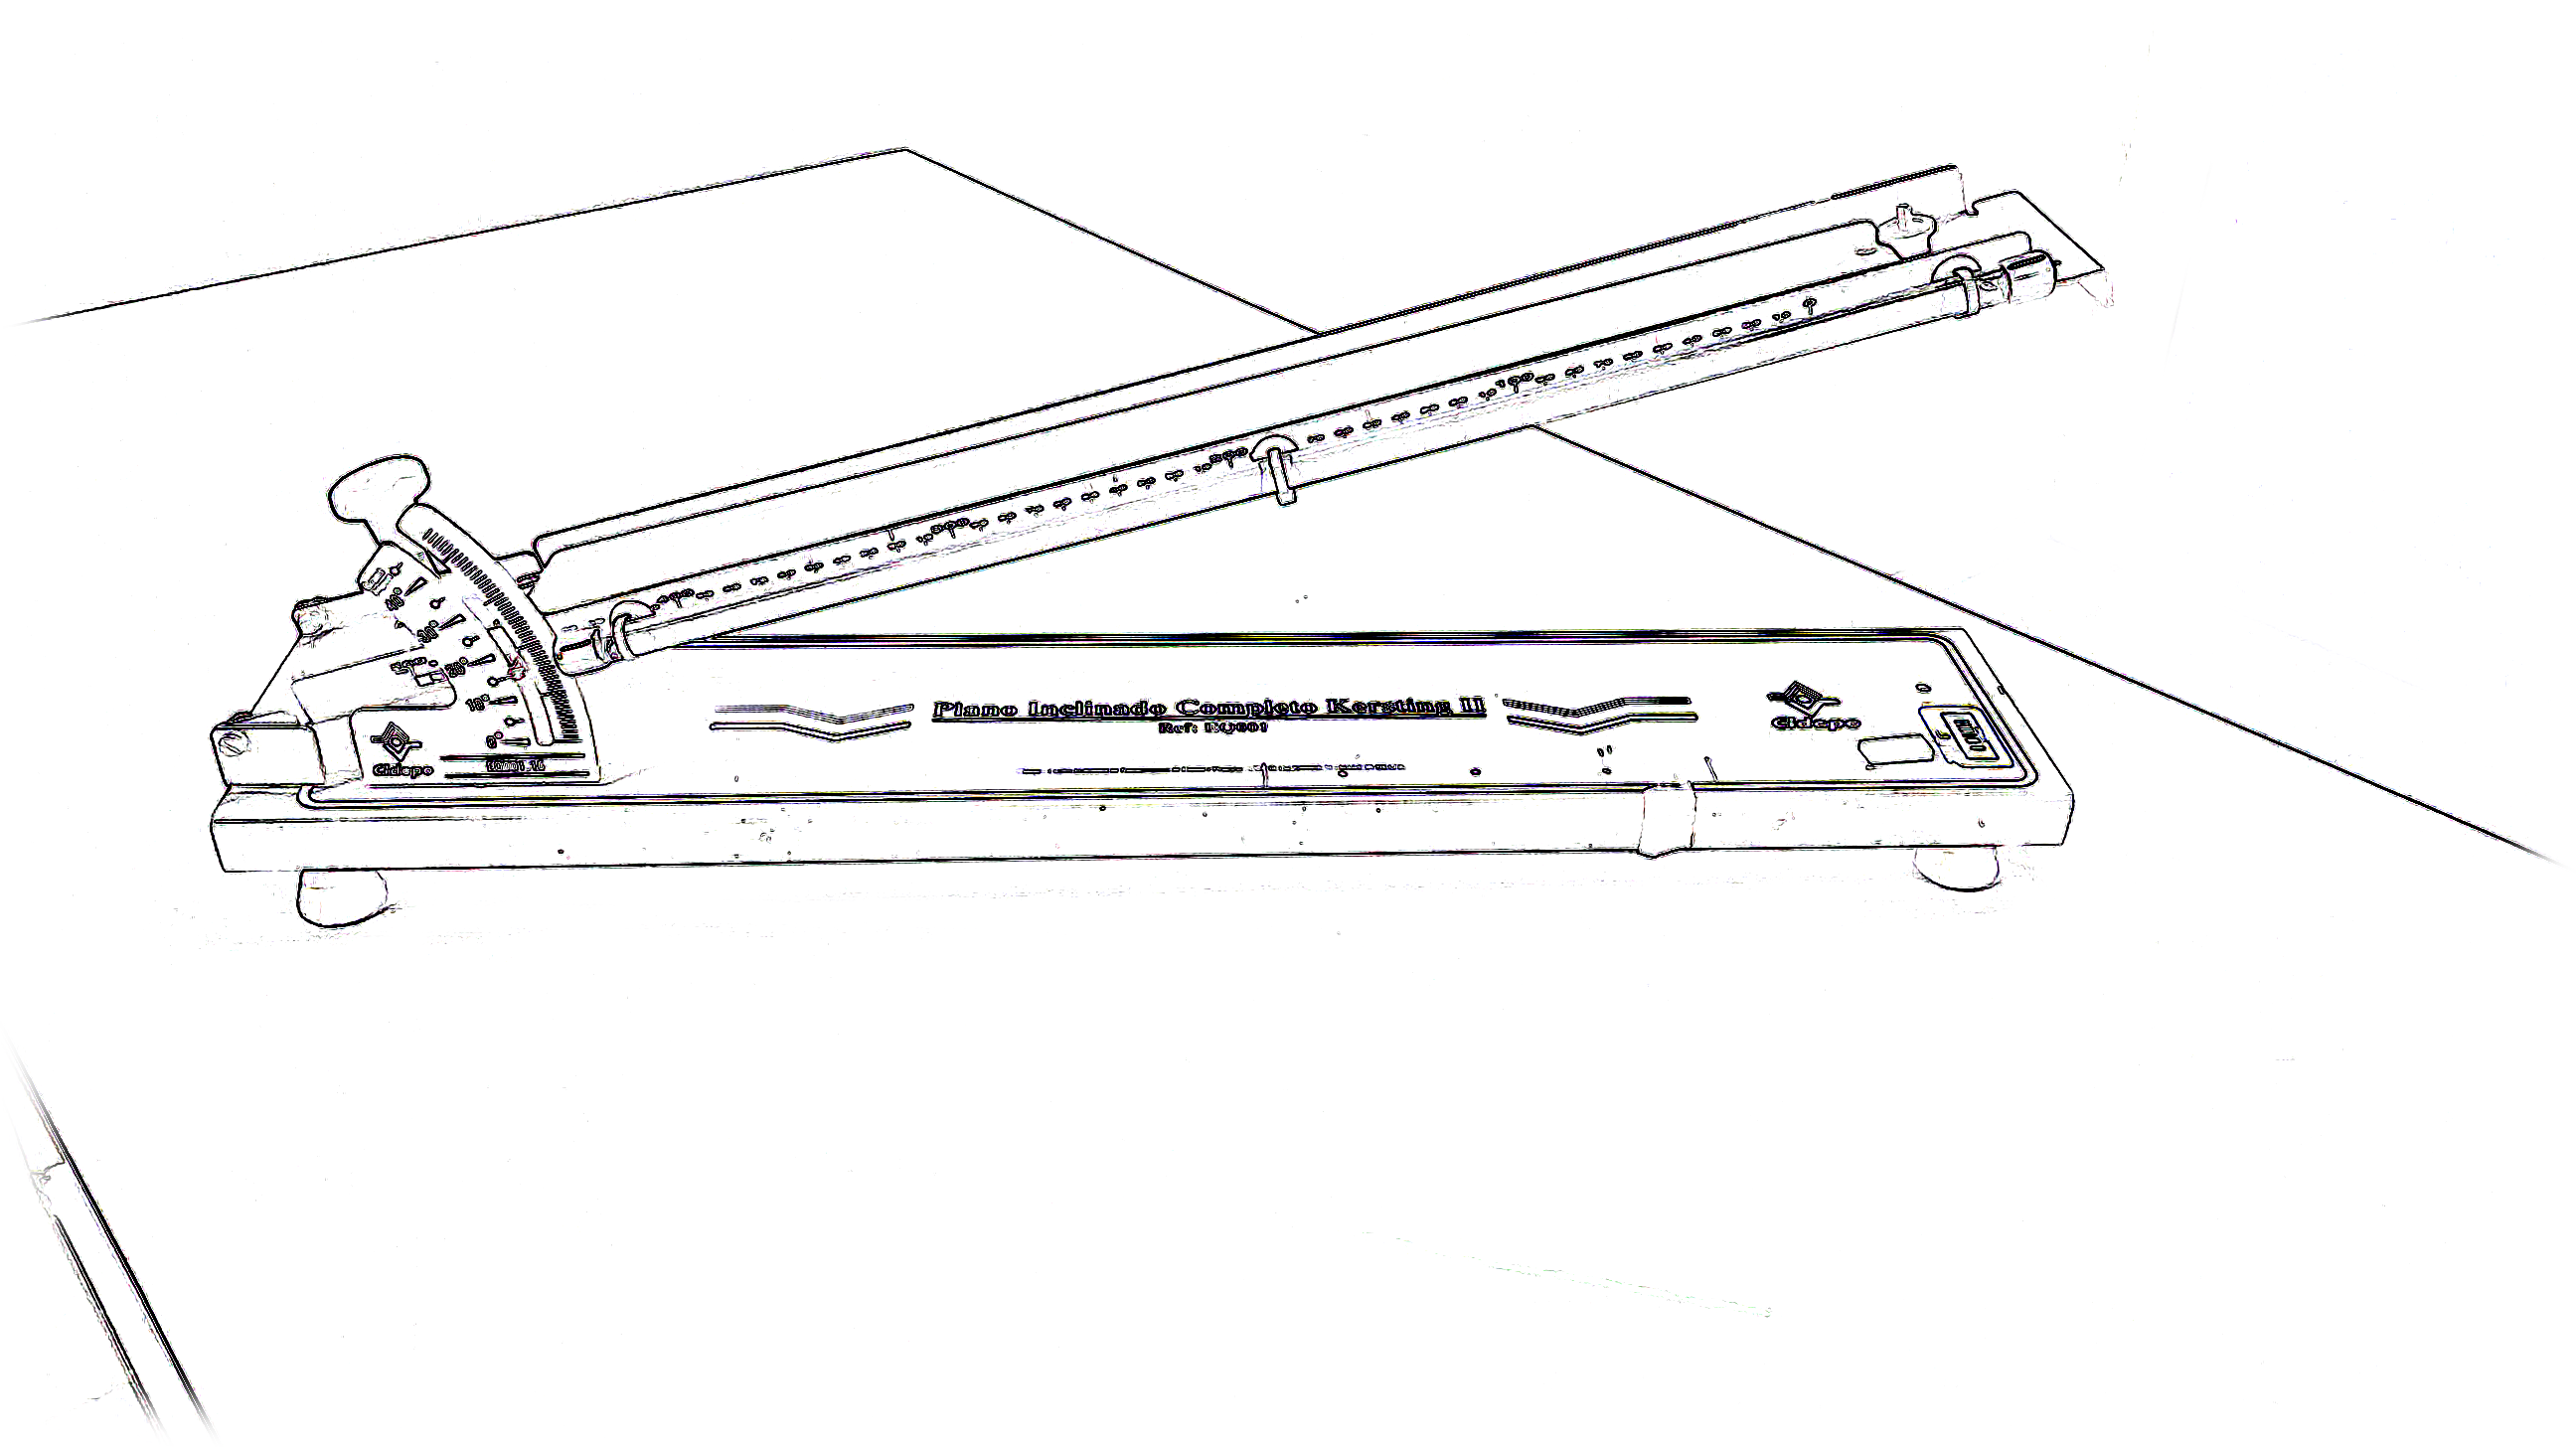
\includegraphics[width=\textwidth]{Ilustrations/Arrasto.png}
	\caption{Plano inclinado com tubo contendo fluido e uma esfera de aço que pode se deslocar.}
\end{marginfigure}

\begin{marginfigure}
\centering
\begin{tikzpicture}[>=Stealth, scale = 1.25]
	\begin{scope}[rotate=30]
%   	\usetikzlibrary{calc}
%   	\def\centerarc[#1](#2)(#3:#4:#5)% [draw options] (center) (initial angle:final angle:radius)
%   	{ \draw[#1] ($(#2)+({#5*cos(#3)},{#5*sin(#3)})$) arc (#3:#4:#5) node[below]{$\theta$}; }
	
	    \draw[dotted,very thin, <-] (-2,0) node[below] {$x$} -- (2,0);
	    \draw[dotted,very thin, ->] (0,-1.5) coordinate (B) -- (0,2) node[left]{$y$};
	    
	    \draw[->] (0,0) coordinate (O) -- node[above right]{$\vec{N}$} (0,0.866025404);
	    \draw[->, dashed] (0,0) -- (-0.5,0) node[above=3pt]{$P_x$};
	    \draw[->, dashed] (0,0) -- (0, -0.866025404) node[right]{$P_y$};
	    \draw[->] (0,0) -- node[below right]{$\vec{F}_a$} (0.5,0);
	    \draw[densely dotted] (-0.5,0) -- (-0.5,-0.866025404);
	    \draw[densely dotted] (-0.5,-0.866025404) -- (0, -0.866025404);
%	    \draw (-0.230940108,-0.4) arc (240:270:0.4619) node[below]{$\theta$};
	\end{scope}
	\draw[fill] (0,0) circle[radius=0.1];
	\draw[->] (0,0) -- (0,-1) node[below left]{$\vec{P}$} coordinate (A);
	
	\pic[draw, "$\theta$", angle radius = 6mm, angle eccentricity = 1.3]{angle=A--O--B};
	
\end{tikzpicture}
\caption{Diagrama de corpo livre da esfera que se desloca dentro do tubo.}
\label{DiagramaEsfera}
\end{marginfigure}

Verificamos para o eixo $y$ que a força normal deve ser equilibrada pela componente $y$ da força peso, pois o objeto não se desloca no eixo $y$ e, portanto, sua aceleração deve ser zero. Já para o eixo $x$, verificamos que
\begin{align}
    F_{R,x} &= m a_x \\
	P_x - F_{a,x} &= ma_x.
\end{align}
%
Substituindo $F_a = b_n v^{n}$, onde $n=1$~ou~$2$ ---~de acordo com as hipóteses discutidas na seção anterior~---, temos
\begin{equation}
	P_x - b_n v^n = ma_x.
\end{equation}

Verificamos então que conforme a velocidade do objeto aumenta, a força de arrasto também aumenta. Isso dá origem a uma \emph{velocidade limite}, isto é, uma velocidade máxima para a qual a força de arrasto equilibra completamente a componente da força peso na direção do eixo $x$. Temos então uma aceleração nula e, portanto, uma velocidade constante. O valor da velocidade terminal pode ser calculado através de
\begin{equation}
	P_x - b_n v_t^n = 0,
\end{equation}
%
ou, substituindo $P_x = Mg\sen\theta$,
\begin{equation}
	v_t^n = \frac{Mg}{b_n}\,\sen\theta.
\end{equation}

A partir do resultado acima, vemos que a velocidade terminal só depende do ângulo $\theta$ de inclinação do tubo, uma vez que os demais parâmetros são constantes. Substituindo os valores de $n$ na equação acima, temos duas hipóteses
\begin{align}
	v_t =\frac{Mg}{b_1}\sen\theta, \qquad\textrm{Hipótese 1} \\
	v_t^2 =\frac{Mg}{b_2}\sen\theta, \qquad\textrm{Hipótese 2.}
\end{align}

Como a velocidade terminal é constante, podemos estabelecer uma posição inicial e uma posição final no tubo cujo tempo de deslocamento possa ser cronometrado. Utilizando uma distância $\Delta x$ fixa, temos então que
\begin{equation}
	v_t = \Delta x / \Delta t.
\end{equation}
%
É importante notar que o objeto já deve ter atingido a velocidade limite antes da posição inicial para que a equação acima seja válida.

%%%%%%%%%%%%%%%%%%%%%%%%%%%%%%%%%%%%%%%%%%%%%%%%%%%%
\subsection{Linearização e teste das duas hipóteses}
%%%%%%%%%%%%%%%%%%%%%%%%%%%%%%%%%%%%%%%%%%%%%%%%%%%%

Para decidirmos qual das hipóteses acima melhor descreve a força de arrasto no experimento, vamos utilizar o coeficiente $r^2$. Para tanto, vamos comparar as duas hipóteses com a equação da reta:
\begin{description}
	\item[Hipótese 1:] Temos nesse caso a seguinte relação entre a equação que rege o fenômeno e a equação da reta:
		\begin{align}
			y &= v_t \\
			A &= 0 \\
			B &= Mg/b_1 \\
			x &= \sen\theta
		\end{align}

	\item[Hipótese 2:] Nesse caso, temos
		\begin{align}
			y &= v_t^2 \\
			A &= 0 \\
			B &= Mg/b_2 \\
			x &= \sen\theta
		\end{align}
\end{description}

%%%%%%%%%%%%%%%%%%%%%%%%%%%%%%%%%%%%%%%%%%%%%%%%%%%%%%%%%%%%%%%%%%%%%%%%%%%%%%%
\section{Experimento}
%%%%%%%%%%%%%%%%%%%%%%%%%%%%%%%%%%%%%%%%%%%%%%%%%%%%%%%%%%%%%%%%%%%%%%%%%%%%%%%

Considerando o movimento de uma esfera em um plano inlinado e sujeita a uma força de arrasto, vamos verificar o tempo necessário para que a ela percorra uma distância preestabelecida, porém para diversos ângulos de inclinação distintos. Para que possamos determinar a velocidade de maneira simples, é necessário que a esfera tenha atingido a velocidade terminal antes de passar pela posição que marca o início do intervalo para o qual mediremos a distância e o tempo. Isso significa que a esfera deve ser solta a partir de um ponto que preceda o ponto inicial por alguns centímetros.\footnote[][-3cm]{Como a esfera tem massa pequena e o fluido é razoavelmente viscoso, a distância necessária é pequena, por volta de \np[cm]{3,00} são suficientes.}

%%%%%%%%%%%%%%%%%%%%%%
\subsection{Objetivos}
%%%%%%%%%%%%%%%%%%%%%%

\begin{itemize}
     \item Verificar a relação entre a força de arrasto e a velocidade;
	 \item Linearizar os conjuntos de dados obtidos e obter os valores de $A$ e $B$ das equações da retas correspondentes;
     \item Elaborar um gráfico $v_t \times \sen\theta$ dos pontos experimentais e adicional a ele a reta obtida através da regressão linear;
	 \item Elaborar um gráfico $v_t^2 \times \sin\theta$ dos pontos experimentais e adicionar a ele a reta obtida através da regressão linear.
\end{itemize}

%%%%%%%%%%%%%%%%%%%%%%%%%%%%%%%%%%%%%%%%%%%%%%%%%%%%%%%%%%%%%%%%%%%%%%%%%%%%%%%
\section{Material Necessário}
%%%%%%%%%%%%%%%%%%%%%%%%%%%%%%%%%%%%%%%%%%%%%%%%%%%%%%%%%%%%%%%%%%%%%%%%%%%%%%%

\begin{itemize}
	\item Plano inclinado;
	\item Cronômetro;
	\item Ímã;
	\item Régua.
\end{itemize}

%%%%%%%%%%%%%%%%%%%%%%%%%%%%%%%%%%%%%%%%%%%%%%%%%%%%%%%%%%%%%%%%%%%%%%%%%%%%%%%
\section{Procedimento Experimental}
%%%%%%%%%%%%%%%%%%%%%%%%%%%%%%%%%%%%%%%%%%%%%%%%%%%%%%%%%%%%%%%%%%%%%%%%%%%%%%%

\begin{enumerate}
	\item Ajuste o plano inclinado para um ângulo de \np[\tcdegree]{5,0}.
	\item Estabeleça o $x_i$ como \np[cm]{10,00}.
	\item Estabeleça o $x_f$ como \np[cm]{40,00}.
	\item Use o ímã para levar a esfera até a posição mais alta do tubo.
	\item Solte a esfera e cronometre o tempo necessário para atravessar a distância entre $x_i$ e $x_f$. Anote o valor na tabela.
	\item Repita a tomada de tempo mais duas vezes para este ângulo.
	\item Aumente o ângulo em \np[\tcdegree]{5,0} e repita os passos acima. Realize este procedimento até atingir o ângulo de \np[\tcdegree]{40,0}.
\end{enumerate}

%%%%%%%%%%%%%%%%%%%%%%%%%%%%%%%%%%%%%%%%%%%%%%%%%%%%%%%%%%%%%%%%%%%%%%%%%%%%%%%
%%%%%%%%%%%%%%%%%%%%%%%%%%%%%%%%%%%%%%%%%%%%%%%%%%%%%%%%%%%%%%%%%%%%%%%%%%%%%%%
%%%%%%%%%%%%%%%%%%%%%%%%%%%%%%%%%%%%%%%%%%%%%%%%%%%%%%%%%%%%%%%%%%%%%%%%%%%%%%%
%%%%%%%%%%%%%%%%%%%%%%%%%%%%%%%%%%%%%%%%%%%%%%%%%%%%%%%%%%%%%%%%%%%%%%%%%%%%%%%
\cleardoublepage

\noindent{}{\huge\textit{Arrasto}}

\vspace{15mm}

\begin{fullwidth}
\noindent{}\makebox[0.6\linewidth]{Turma:\enspace\hrulefill}\makebox[0.4\textwidth]{  Data:\enspace\hrulefill}
\vspace{5mm}

\noindent{}\makebox[0.6\linewidth]{Aluno(a):\enspace\hrulefill}\makebox[0.4\textwidth]{  Matrícula:\enspace\hrulefill}

\noindent{}\makebox[0.6\linewidth]{Aluno(a):\enspace\hrulefill}\makebox[0.4\textwidth]{  Matrícula:\enspace\hrulefill}

\noindent{}\makebox[0.6\linewidth]{Aluno(a):\enspace\hrulefill}\makebox[0.4\textwidth]{  Matrícula:\enspace\hrulefill}

\noindent{}\makebox[0.6\linewidth]{Aluno(a):\enspace\hrulefill}\makebox[0.4\textwidth]{  Matrícula:\enspace\hrulefill}

\noindent{}\makebox[0.6\linewidth]{Aluno(a):\enspace\hrulefill}\makebox[0.4\textwidth]{  Matrícula:\enspace\hrulefill}
\end{fullwidth}

\vspace{5mm}

%%%%%%%%%%%%%%%%%%%%%%%%%%%%%%%%%%%%%%%%%%%%%%%%%%%%%%%%%%%%%%%%%%%%%%%%%%%%%%%
\section{Questionário}
%%%%%%%%%%%%%%%%%%%%%%%%%%%%%%%%%%%%%%%%%%%%%%%%%%%%%%%%%%%%%%%%%%%%%%%%%%%%%%%

\begin{question}[type={exam}]{1}
Apresente os resultados de maneira clara e organizada. Mostre os cálculos requisitados de maneira clara e sucinta, evidenciando o raciocínio desenvolvido.
\end{question}

\begin{question}[type={exam}]{1}
Preencha as colunas de dados das tabelas com o número adequado de algarismos significativos e unidades.
\end{question}


\begin{question}[type={exam}]{3}
Elabore um gráfico $v_t \times \sen\theta$ dos pontos experimentais e um gráfico de $v_t^2 \times \sen\theta$.
\end{question}

\begin{question}[type={exam}]{3}
Através dos gráficos elaborados no item anterior, para ambos os conjuntos de dados, obtenha os valores de $A$, $B$ e $r^2$ da melhor reta correspondente (a reta da regressão linear). Adicione essa reta ao gráfico e coloque a equação da reta, juntamente com o coeficiente $r^2$ na legenda.
\end{question}

\begin{question}[type={exam}]{2}
Através da análise do coeficiente de dispersão linear $r^2$, indique qual das hipóteses discutidas na Seção~\ref{SecaoF_a} melhor descreve o fenômeno.
\end{question}
\vfill

%%%%%%%%%%%%%%%%%%%%%%%%%%%%%%%%%%%%%%%%%%%%%%%%%%%%%%%%%%%%%%%%%%%%%%%%%%%%%%%
\pagebreak
\section{Tabelas}
%%%%%%%%%%%%%%%%%%%%%%%%%%%%%%%%%%%%%%%%%%%%%%%%%%%%%%%%%%%%%%%%%%%%%%%%%%%%%%%

\begin{table*}[!h]
\centering
\begin{tabular}{lp{25mm}p{25mm}p{25mm}p{25mm}p{25mm}l}
\toprule
	& \multicolumn{2}{l}{\textbf{Posições inicial e final}} \\
	\cmidrule{2-3}
	& $x_i$ \cellcolor[gray]{0.89} & \cellcolor[gray]{0.92} \\
	& $x_f$ \cellcolor[gray]{0.95} & \cellcolor[gray]{0.97} \\
	\cmidrule{2-3}
\\
	& \multicolumn{6}{l}{\textbf{Dados experimentais}} \\
	\cmidrule{2-6}
	& $t_1$ & $t_2$ & $t_3$ & $\overline{t}$ & $\theta$ & \\
	\cmidrule{2-6}
	& \cellcolor[gray]{0.89} & \cellcolor[gray]{0.92} & \cellcolor[gray]{0.89} & \cellcolor[gray]{0.92} & \cellcolor[gray]{0.89} \\
	& \cellcolor[gray]{0.95} & \cellcolor[gray]{0.97} & \cellcolor[gray]{0.95} & \cellcolor[gray]{0.97} & \cellcolor[gray]{0.95} \\
	& \cellcolor[gray]{0.89} & \cellcolor[gray]{0.92} & \cellcolor[gray]{0.89} & \cellcolor[gray]{0.92} & \cellcolor[gray]{0.89} \\
	& \cellcolor[gray]{0.95} & \cellcolor[gray]{0.97} & \cellcolor[gray]{0.95} & \cellcolor[gray]{0.97} & \cellcolor[gray]{0.95} \\
	& \cellcolor[gray]{0.89} & \cellcolor[gray]{0.92} & \cellcolor[gray]{0.89} & \cellcolor[gray]{0.92} & \cellcolor[gray]{0.89} \\
	& \cellcolor[gray]{0.95} & \cellcolor[gray]{0.97} & \cellcolor[gray]{0.95} & \cellcolor[gray]{0.97} & \cellcolor[gray]{0.95} \\
	& \cellcolor[gray]{0.89} & \cellcolor[gray]{0.92} & \cellcolor[gray]{0.89} & \cellcolor[gray]{0.92} & \cellcolor[gray]{0.89} \\
	& \cellcolor[gray]{0.95} & \cellcolor[gray]{0.97} & \cellcolor[gray]{0.95} & \cellcolor[gray]{0.97} & \cellcolor[gray]{0.95} \\
	& \cellcolor[gray]{0.89} & \cellcolor[gray]{0.92} & \cellcolor[gray]{0.89} & \cellcolor[gray]{0.92} & \cellcolor[gray]{0.89} \\
	& \cellcolor[gray]{0.95} & \cellcolor[gray]{0.97} & \cellcolor[gray]{0.95} & \cellcolor[gray]{0.97} & \cellcolor[gray]{0.95} \\
	& \cellcolor[gray]{0.89} & \cellcolor[gray]{0.92} & \cellcolor[gray]{0.89} & \cellcolor[gray]{0.92} & \cellcolor[gray]{0.89} \\
	& \cellcolor[gray]{0.95} & \cellcolor[gray]{0.97} & \cellcolor[gray]{0.95} & \cellcolor[gray]{0.97} & \cellcolor[gray]{0.95} \\
	\cmidrule{2-6}
\\
	& \multicolumn{2}{l}{\textbf{Dados para o gráfico}} \\
	\cmidrule{2-3}
	& $v_t$ & $\sen\theta$ \\
	\cmidrule{2-3}
	& \cellcolor[gray]{0.89} & \cellcolor[gray]{0.92} \\
	& \cellcolor[gray]{0.95} & \cellcolor[gray]{0.97} \\
	& \cellcolor[gray]{0.89} & \cellcolor[gray]{0.92} \\
	& \cellcolor[gray]{0.95} & \cellcolor[gray]{0.97} \\
	& \cellcolor[gray]{0.89} & \cellcolor[gray]{0.92} \\
	& \cellcolor[gray]{0.95} & \cellcolor[gray]{0.97} \\
	& \cellcolor[gray]{0.89} & \cellcolor[gray]{0.92} \\
	& \cellcolor[gray]{0.95} & \cellcolor[gray]{0.97} \\
	& \cellcolor[gray]{0.89} & \cellcolor[gray]{0.92} \\
	& \cellcolor[gray]{0.95} & \cellcolor[gray]{0.97} \\
	& \cellcolor[gray]{0.89} & \cellcolor[gray]{0.92} \\
	& \cellcolor[gray]{0.95} & \cellcolor[gray]{0.97} \\
	\cmidrule{2-3}
\bottomrule
\end{tabular}
\caption[][5mm]{Dados para o movimento efetuado pela esfera sob ação da gravidade e do arrasto.}
\label{TabelaDados}
\end{table*}

%%%%%%%%%%%%%%%%%%%%%%%%%%%%%%%%%%%%%%%%%%%%%%%%%%%%%%%%%%%%%%%%%%%%%%%%%%%%%%%
\chapter{Elasticidade}
\label{Chap:ExpElasticidade}
%%%%%%%%%%%%%%%%%%%%%%%%%%%%%%%%%%%%%%%%%%%%%%%%%%%%%%%%%%%%%%%%%%%%%%%%%%%%%%%

\begin{fullwidth}\it
	Realizaremos um experimento visando mostrar o comportamento não-linear de um corpo que sofre uma deformação. Verificaremos através dos dados que a deformação segue uma forma característica conhecida como \emph{curva de histerese}. Veremos que as deformações com dependência linear na força aplicada se restringem a condições muito específicas. Utilizaremos os seguintes conceitos/técnicas de análise de dados: medidas, algarismos significativos, gráficos, erros de escala e propagados, histogramas e desvio padrão.
\end{fullwidth}

%%%%%%%%%%%%%%%%%%%%%%%%%%%%%%%%%%%%%%%%%%%%%%%%%%%%%%%%%%%%%%%%%%%%%%%%%%%%%%%
\section{Elasticidade}
%%%%%%%%%%%%%%%%%%%%%%%%%%%%%%%%%%%%%%%%%%%%%%%%%%%%%%%%%%%%%%%%%%%%%%%%%%%%%%%

\begin{marginfigure}[7cm]
	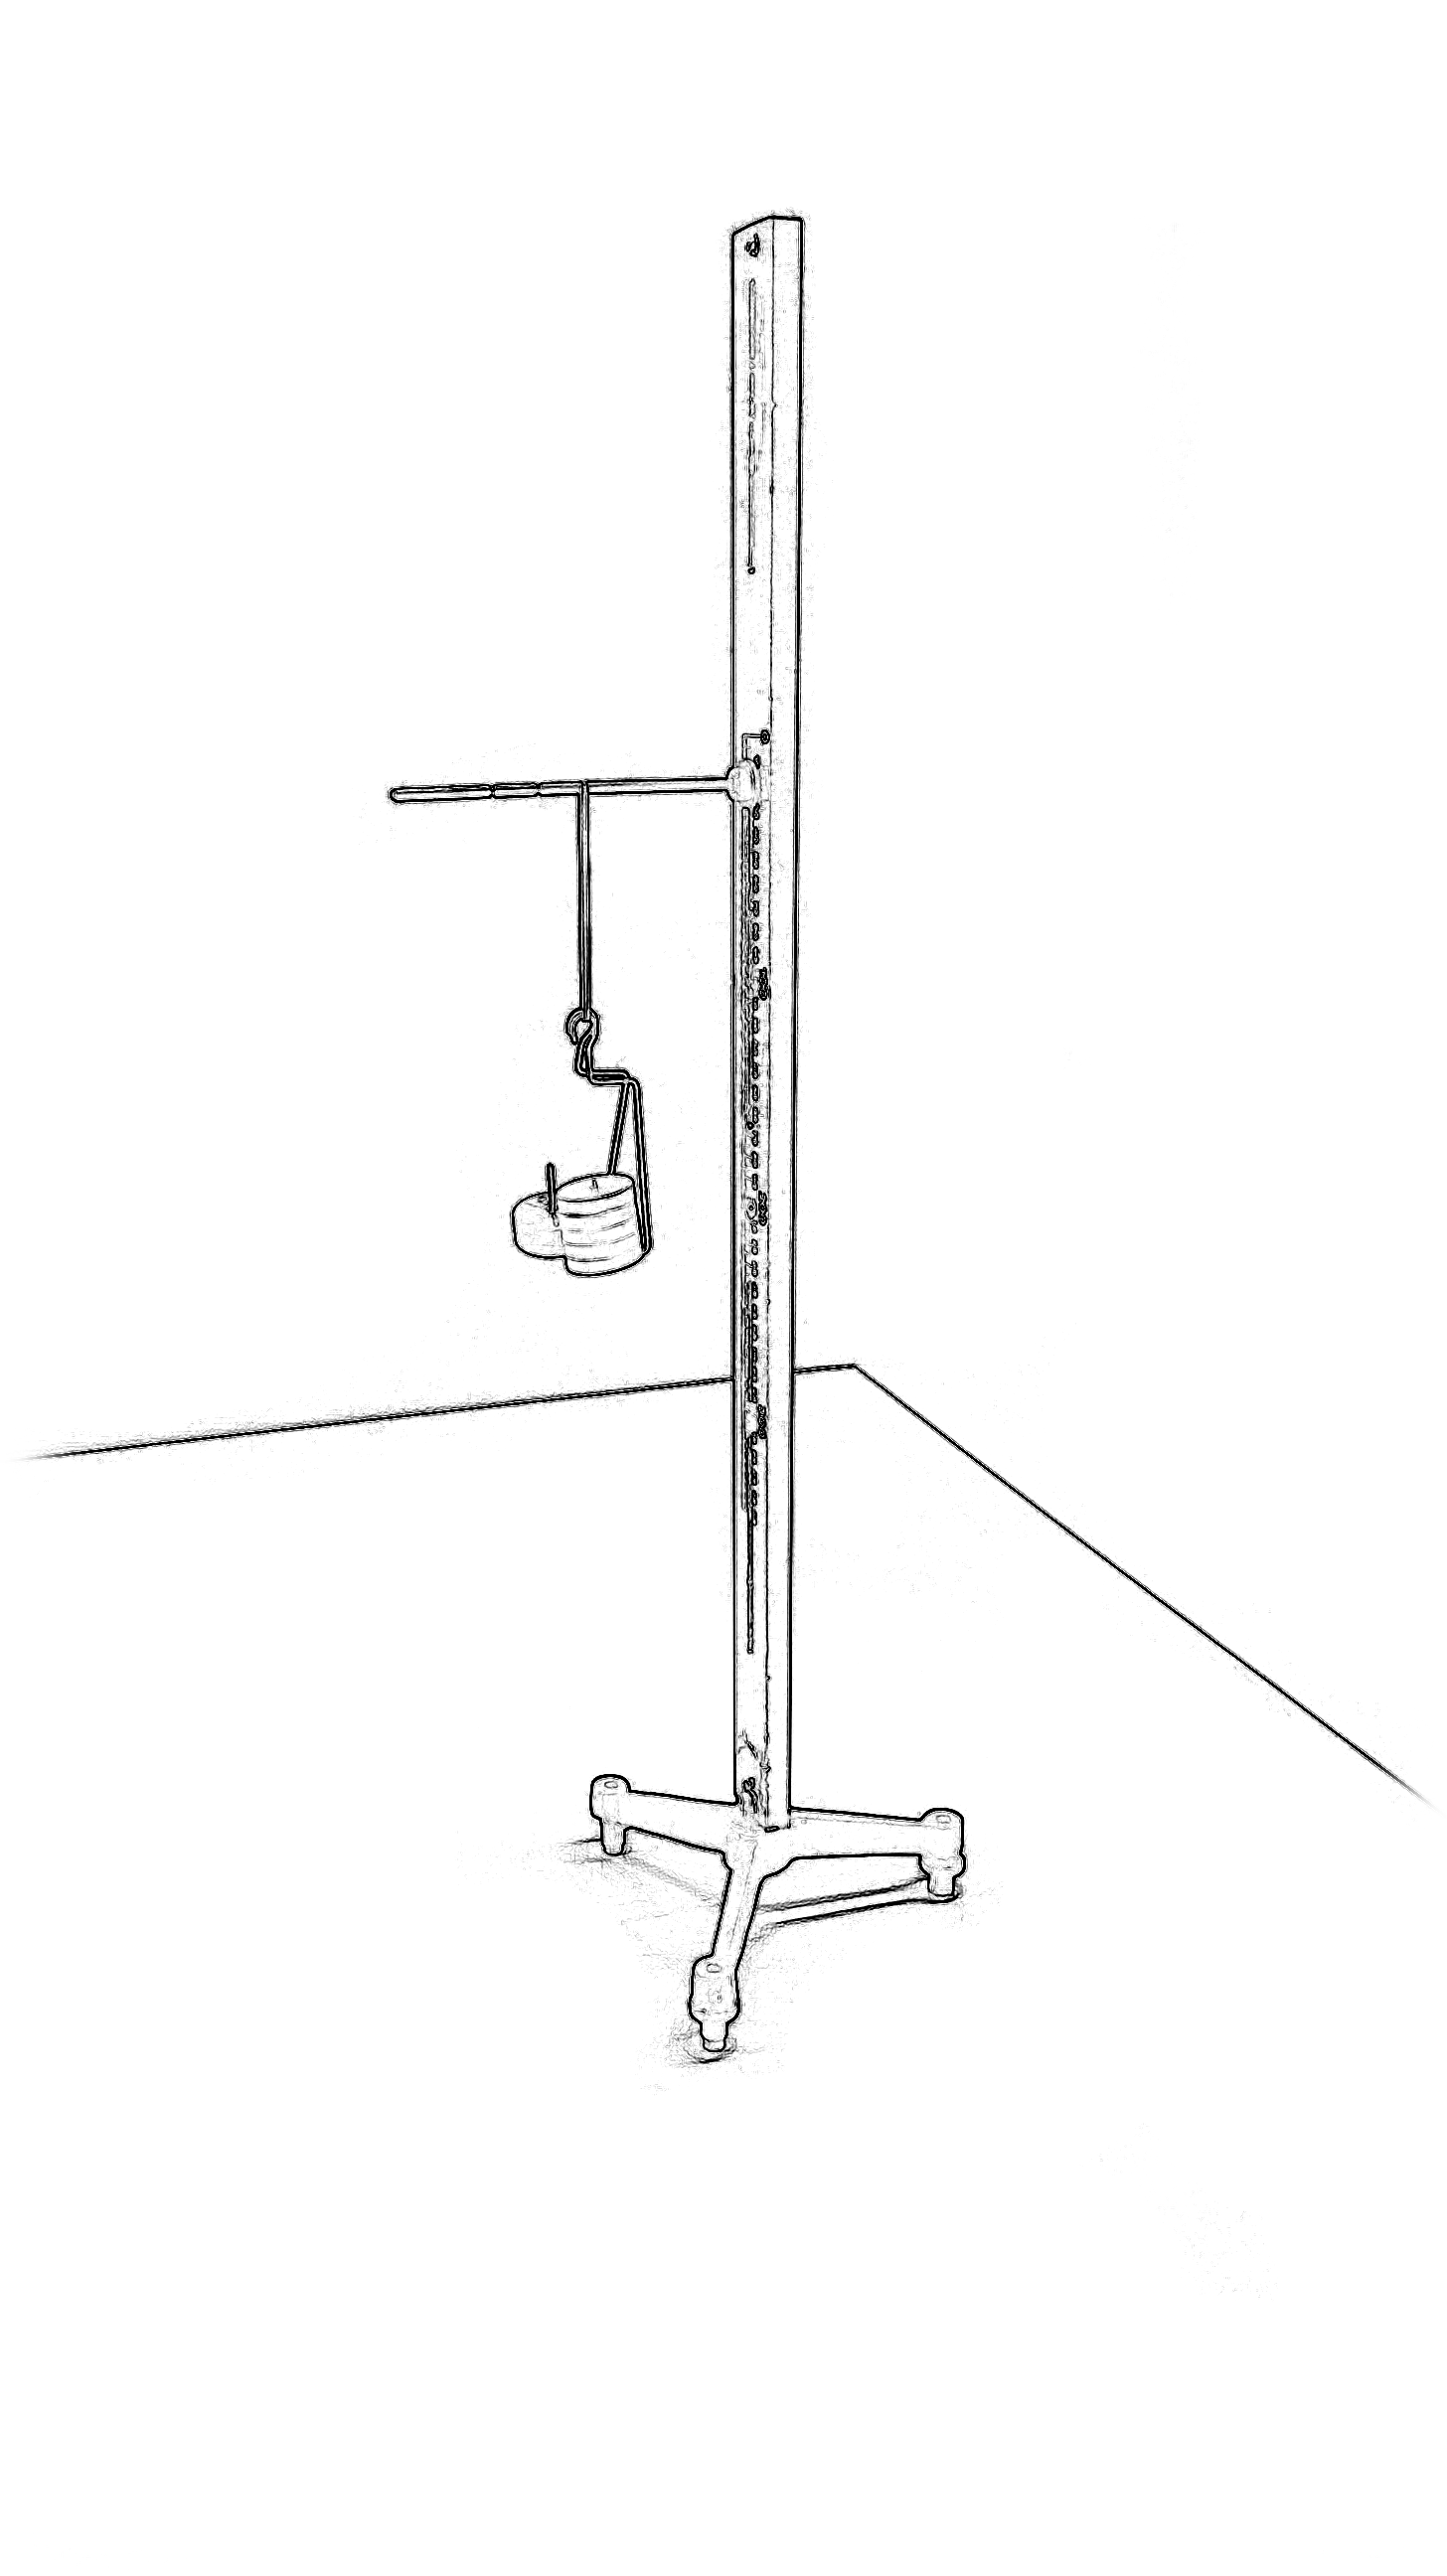
\includegraphics[width=\textwidth]{Ilustrations/Elasticidade.png}
	\caption{Ao submetermos um elástico a uma força variável, verificando a distensão registrada em função da força, obtemos uma \emph{curva de histerese}.}
\end{marginfigure}

Verificamos através da Lei de Hooke que a deformação de objetos em resposta a uma força aplicada é proporcional à intensidade da força:
\begin{equation}
	\Delta x = \frac{F}{k}.
\end{equation}

\noindent{}Sabemos, no entanto, que um objeto sujeito a uma força muito grande pode apresentar uma deformação permanente, ou mesmo se quebrar. Além disso, no caso mais geral, a deformação pode ser \emph{não-linear}.

Mesmo para uma mola, caso clássico em que se aplica a Lei de Hooke, a deformação será não-linear se a distensão da mola for muito grande. Por isso se faz a restrição de que \emph{a distensão da mola deve ser pequena}. Podemos entender melhor essa restrição chamando a força exercida pela mola de $f(x)$, onde $x$ representa a distensão da mola, e fazendo uma expansão de $f(x)$ em uma \emph{série de Taylor}. A expansão em série de Taylor nos que diz que uma função $g(x)$ qualquer pode ser aproximada em torno de um ponto $x=a$ qualquer como
\begin{equation}
	g(x) = g(a) + g'(a)(x - a) + g''(a)(x-a)^2 + g'''(a)(x-a)^3 + \dots,
\end{equation}
onde $g'(a)$, $g''(a)$, $g'''(a)$, etc. são as derivadas da função $g(x)$ calculadas no ponto $a$.

Assim, podemos expandir a função $f(x)$ em torno de zero (considerando que esta é a posição de equilíbrio) como
\begin{equation}
	f(x) = f(0) + f'(0) (x-0) + f''(0)(x-0)^2 + \dots.
\end{equation}
%
No entanto, $f(0)$ é a força na posição de equilíbrio, ou seja, zero. Além disso, se $x$ é muito pequeno, temos que $x^2$ é menor ainda e por isso podemos desprezar todos os termos de ordem 2 (termos quadráticos) ou maior. Obtemos então:
\begin{equation}
	f(x) = f'(0)x,
\end{equation}
%
e se fizermos $k \equiv f'(0)$,
\begin{equation}
	f(x) = kx.
\end{equation}
%
\textbf{Portanto, quando falamos em pequenos deslocamentos, estamos restringindo os valores de termos de ordens quadrática ou superiores a valores muito menores que o termo de ordem linear}. Respeitada essa condição, o que poder ser feito através da escolha de uma distensão máxima adequada -- isto é, que ela seja suficientemente pequena para que os termos de ordem superior a 2 sejam desprezíveis --, podemos tratar as deformações de um objeto como sendo lineares.

%%%%%%%%%%%%%%%%%%%%%%%%%%%%%%%%%%%%%
\subsection{Elasticidade e Histerese}
%%%%%%%%%%%%%%%%%%%%%%%%%%%%%%%%%%%%%

\begin{marginfigure}
	\centering
	\begin{tikzpicture}[scale=0.3, >=Stealth]
		\draw[very thin, ->] (-5,-4) -- +(10,0);
		\draw[very thin, ->] (-5,-4) -- +(0,8);
		\clip (-4,-4) rectangle (4,4);
		\draw[thick] (-5,-3) -- (-4,-3) to [controls={+(3,0) and +(-3,0)}] (2,3) -- (5,3);
		\draw[thick] (5,3) -- (4,3) to [controls={+(-3,0) and +(3,0)}] (-2,-3) -- (-5,-3);
	\end{tikzpicture}
	\caption{Gráfico típico de um fenômeno de histerese.}
	\label{Fig:Histerese}
\end{marginfigure}

Uma característica que também pode ser observada no caso de uma deformação não linear é a \emph{histerese}. Temos na Figura~\ref{Fig:Histerese} uma típica figura de histerese: quando efetuamos um aumento gradual da variável independente, ocorre um aumento não linear da variável dependente. Quando passamos a fazer uma diminuição da variável independente, existe uma diminuição da variável dependente, porémos valores assumidos pela variável dependente são diferentes nos dois processos. Vários sistemas físicos têm esse tipo de comportamento: deformações de materiais, magnetização de imãs, campos elétricos em alguns materiais, etc.

\begin{figure*}[!htb]
	\centering
	\begin{tikzpicture}[gnuplot]
%% generated with GNUPLOT 5.0p0 (Lua 5.3; terminal rev. 99, script rev. 100)
%% 2015-07-06T11:33:50 BRT
\path (0.000,0.000) rectangle (14.000,9.000);
\gpcolor{color=gp lt color border}
\gpsetlinetype{gp lt border}
\gpsetdashtype{gp dt solid}
\gpsetlinewidth{1.00}
\draw[gp path] (1.136,1.268)--(1.316,1.268);
\draw[gp path] (13.447,1.268)--(13.267,1.268);
\node[gp node right] at (0.952,1.268) {$15$};
\draw[gp path] (1.136,2.684)--(1.316,2.684);
\draw[gp path] (13.447,2.684)--(13.267,2.684);
\node[gp node right] at (0.952,2.684) {$20$};
\draw[gp path] (1.136,4.100)--(1.316,4.100);
\draw[gp path] (13.447,4.100)--(13.267,4.100);
\node[gp node right] at (0.952,4.100) {$25$};
\draw[gp path] (1.136,5.516)--(1.316,5.516);
\draw[gp path] (13.447,5.516)--(13.267,5.516);
\node[gp node right] at (0.952,5.516) {$30$};
\draw[gp path] (1.136,6.932)--(1.316,6.932);
\draw[gp path] (13.447,6.932)--(13.267,6.932);
\node[gp node right] at (0.952,6.932) {$35$};
\draw[gp path] (1.136,8.348)--(1.316,8.348);
\draw[gp path] (13.447,8.348)--(13.267,8.348);
\node[gp node right] at (0.952,8.348) {$40$};
\draw[gp path] (1.649,0.985)--(1.649,1.165);
\draw[gp path] (1.649,8.631)--(1.649,8.451);
\node[gp node center] at (1.649,0.677) {$0$};
\draw[gp path] (3.701,0.985)--(3.701,1.165);
\draw[gp path] (3.701,8.631)--(3.701,8.451);
\node[gp node center] at (3.701,0.677) {$200$};
\draw[gp path] (5.753,0.985)--(5.753,1.165);
\draw[gp path] (5.753,8.631)--(5.753,8.451);
\node[gp node center] at (5.753,0.677) {$400$};
\draw[gp path] (7.804,0.985)--(7.804,1.165);
\draw[gp path] (7.804,8.631)--(7.804,8.451);
\node[gp node center] at (7.804,0.677) {$600$};
\draw[gp path] (9.856,0.985)--(9.856,1.165);
\draw[gp path] (9.856,8.631)--(9.856,8.451);
\node[gp node center] at (9.856,0.677) {$800$};
\draw[gp path] (11.908,0.985)--(11.908,1.165);
\draw[gp path] (11.908,8.631)--(11.908,8.451);
\node[gp node center] at (11.908,0.677) {$1000$};
\draw[gp path] (1.136,8.631)--(1.136,0.985)--(13.447,0.985)--(13.447,8.631)--cycle;
\node[gp node center,rotate=-270] at (0.246,4.808) {$L$~(cm)};
\node[gp node center] at (7.291,0.215) {$m$~(g)};
\node[gp node left] at (2.604,8.297) {carga};
\gpcolor{rgb color={0.000,0.000,0.000}}
\gpsetlinewidth{2.00}
\gpsetpointsize{4.00}
\gppoint{gp mark 9}{(2.235,1.835)}
\gppoint{gp mark 9}{(2.747,1.948)}
\gppoint{gp mark 9}{(3.259,2.004)}
\gppoint{gp mark 9}{(3.771,2.146)}
\gppoint{gp mark 9}{(4.273,2.259)}
\gppoint{gp mark 9}{(4.870,2.373)}
\gppoint{gp mark 9}{(5.374,2.571)}
\gppoint{gp mark 9}{(5.887,2.741)}
\gppoint{gp mark 9}{(6.399,2.967)}
\gppoint{gp mark 9}{(6.902,3.222)}
\gppoint{gp mark 9}{(7.481,3.647)}
\gppoint{gp mark 9}{(7.990,4.015)}
\gppoint{gp mark 9}{(8.504,4.553)}
\gppoint{gp mark 9}{(9.014,4.950)}
\gppoint{gp mark 9}{(9.527,5.374)}
\gppoint{gp mark 9}{(10.114,5.941)}
\gppoint{gp mark 9}{(10.627,6.252)}
\gppoint{gp mark 9}{(11.140,6.649)}
\gppoint{gp mark 9}{(11.653,7.130)}
\gppoint{gp mark 9}{(12.160,7.272)}
\gppoint{gp mark 9}{(1.962,8.297)}
\draw[gp path] (2.235,1.838)--(2.335,1.857)--(2.435,1.877)--(2.536,1.896)--(2.636,1.914)%
  --(2.736,1.932)--(2.836,1.949)--(2.937,1.966)--(3.037,1.983)--(3.137,2.001)--(3.237,2.019)%
  --(3.338,2.039)--(3.438,2.061)--(3.538,2.083)--(3.638,2.107)--(3.739,2.130)--(3.839,2.153)%
  --(3.939,2.176)--(4.039,2.198)--(4.140,2.221)--(4.240,2.243)--(4.340,2.265)--(4.440,2.286)%
  --(4.541,2.309)--(4.641,2.332)--(4.741,2.357)--(4.841,2.384)--(4.942,2.413)--(5.042,2.444)%
  --(5.142,2.477)--(5.242,2.510)--(5.343,2.545)--(5.443,2.580)--(5.543,2.616)--(5.643,2.652)%
  --(5.744,2.689)--(5.844,2.727)--(5.944,2.766)--(6.044,2.807)--(6.145,2.849)--(6.245,2.893)%
  --(6.345,2.939)--(6.445,2.986)--(6.546,3.036)--(6.646,3.088)--(6.746,3.143)--(6.846,3.201)%
  --(6.947,3.262)--(7.047,3.326)--(7.147,3.393)--(7.247,3.463)--(7.348,3.535)--(7.448,3.609)%
  --(7.548,3.685)--(7.648,3.763)--(7.749,3.843)--(7.849,3.925)--(7.949,4.011)--(8.049,4.099)%
  --(8.150,4.190)--(8.250,4.283)--(8.350,4.376)--(8.450,4.469)--(8.551,4.559)--(8.651,4.648)%
  --(8.751,4.734)--(8.852,4.820)--(8.952,4.905)--(9.052,4.989)--(9.152,5.074)--(9.253,5.159)%
  --(9.353,5.245)--(9.453,5.332)--(9.553,5.419)--(9.654,5.507)--(9.754,5.595)--(9.854,5.683)%
  --(9.954,5.769)--(10.055,5.852)--(10.155,5.932)--(10.255,6.008)--(10.355,6.082)--(10.456,6.156)%
  --(10.556,6.229)--(10.656,6.303)--(10.756,6.378)--(10.857,6.455)--(10.957,6.534)--(11.057,6.613)%
  --(11.157,6.693)--(11.258,6.774)--(11.358,6.853)--(11.458,6.929)--(11.558,7.000)--(11.659,7.065)%
  --(11.759,7.122)--(11.859,7.173)--(11.959,7.220)--(12.060,7.263)--(12.160,7.305);
\gpcolor{color=gp lt color border}
\node[gp node left] at (2.604,7.989) {descarga};
\gpcolor{rgb color={0.000,0.000,0.000}}
\gppoint{gp mark 11}{(12.160,7.272)}
\gppoint{gp mark 11}{(11.653,7.328)}
\gppoint{gp mark 11}{(11.140,7.272)}
\gppoint{gp mark 11}{(10.627,7.215)}
\gppoint{gp mark 11}{(10.114,7.158)}
\gppoint{gp mark 11}{(9.527,7.045)}
\gppoint{gp mark 11}{(9.014,6.960)}
\gppoint{gp mark 11}{(8.504,6.819)}
\gppoint{gp mark 11}{(7.990,6.677)}
\gppoint{gp mark 11}{(7.481,6.450)}
\gppoint{gp mark 11}{(6.902,6.139)}
\gppoint{gp mark 11}{(6.399,5.799)}
\gppoint{gp mark 11}{(5.887,5.374)}
\gppoint{gp mark 11}{(5.374,4.950)}
\gppoint{gp mark 11}{(4.870,4.468)}
\gppoint{gp mark 11}{(4.273,3.789)}
\gppoint{gp mark 11}{(3.771,3.449)}
\gppoint{gp mark 11}{(3.259,3.109)}
\gppoint{gp mark 11}{(2.747,2.712)}
\gppoint{gp mark 11}{(2.235,2.401)}
\gppoint{gp mark 11}{(1.962,7.989)}
\draw[gp path] (2.235,2.394)--(2.335,2.459)--(2.435,2.524)--(2.536,2.589)--(2.636,2.655)%
  --(2.736,2.722)--(2.836,2.791)--(2.937,2.861)--(3.037,2.931)--(3.137,3.002)--(3.237,3.072)%
  --(3.338,3.141)--(3.438,3.210)--(3.538,3.279)--(3.638,3.348)--(3.739,3.418)--(3.839,3.489)%
  --(3.939,3.563)--(4.039,3.640)--(4.140,3.721)--(4.240,3.807)--(4.340,3.899)--(4.440,3.997)%
  --(4.541,4.098)--(4.641,4.202)--(4.741,4.307)--(4.841,4.412)--(4.942,4.516)--(5.042,4.618)%
  --(5.142,4.718)--(5.242,4.815)--(5.343,4.910)--(5.443,5.002)--(5.543,5.092)--(5.643,5.180)%
  --(5.744,5.266)--(5.844,5.351)--(5.944,5.435)--(6.044,5.517)--(6.145,5.598)--(6.245,5.677)%
  --(6.345,5.754)--(6.445,5.828)--(6.546,5.901)--(6.646,5.970)--(6.746,6.038)--(6.846,6.102)%
  --(6.947,6.164)--(7.047,6.224)--(7.147,6.281)--(7.247,6.335)--(7.348,6.388)--(7.448,6.438)%
  --(7.548,6.485)--(7.648,6.531)--(7.749,6.574)--(7.849,6.615)--(7.949,6.653)--(8.049,6.689)%
  --(8.150,6.723)--(8.250,6.754)--(8.350,6.784)--(8.450,6.813)--(8.551,6.840)--(8.651,6.867)%
  --(8.751,6.892)--(8.852,6.916)--(8.952,6.940)--(9.052,6.962)--(9.152,6.982)--(9.253,7.002)%
  --(9.353,7.021)--(9.453,7.040)--(9.553,7.058)--(9.654,7.076)--(9.754,7.093)--(9.854,7.111)%
  --(9.954,7.127)--(10.055,7.143)--(10.155,7.159)--(10.255,7.173)--(10.355,7.186)--(10.456,7.199)%
  --(10.556,7.212)--(10.656,7.224)--(10.756,7.236)--(10.857,7.248)--(10.957,7.259)--(11.057,7.270)%
  --(11.157,7.280)--(11.258,7.288)--(11.358,7.296)--(11.458,7.302)--(11.558,7.306)--(11.659,7.307)%
  --(11.759,7.306)--(11.859,7.303)--(11.959,7.297)--(12.060,7.291)--(12.160,7.284);
\gpcolor{color=gp lt color border}
\gpsetlinewidth{1.00}
\draw[gp path] (1.136,8.631)--(1.136,0.985)--(13.447,0.985)--(13.447,8.631)--cycle;
%% coordinates of the plot area
\gpdefrectangularnode{gp plot 1}{\pgfpoint{1.136cm}{0.985cm}}{\pgfpoint{13.447cm}{8.631cm}}
\end{tikzpicture}
%% gnuplot variables

	\caption{Gráfico de histerese para o processo de carregamento e descarregamento de um elástico. Note que o último ponto do processo de carga e o primeiro do processo de descarga coincidem.}
	\label{Fig:HistereseElast}
\end{figure*}

Na Figura~\ref{Fig:HistereseElast} temos gráfico da tensão em função deformação para um elástico de borracha. As linhas representam o processo de aumento e diminuição progressiva da tensão exercida sobre o elástico. Vemos que as duas curvas não coincidem. É impotante notar que, para o caso elástico, só há a coincidência entre o ponto inicial e final se o processo for realizado lentamente.

A explicação para este fenômeno pode ser dada ao analisarmos a energia armazenada no elástico. Em uma mola, quando a esticamos, armazenamos energia potencial elástica. Essa é praticamente a única forma de energia armazenada. Já para um elástico de borracha, quando o esticamos, armazenamos energia potencial elástica, no entanto, também é possível notar um \textbf{aquecimento do elástico}. Quando esticamos o elástico, ele sofre uma aumento de temperatura, perdendo calor para o ambiente. Ao ser relaxado, é necessária a absorção de calor do meio. Como esse processo é demorado, se relaxarmos o elástico rapidamente, percebemos que ele não volta ao tamanho original. Após algum tempo, no entanto, o elástico absorve o calor do meio e volta ao tamanho original.

Esse fenômeno pode ser entendido analisando a estrutura da borracha: ela é constituída de moléculas de polímeros de tamanhos diferentes, constituindo um emaranhado de fibras. Devido à agitação térmica das moléculas -- agitação característica dos corpos a nível molecular associada à temperatura -- as moléculas sofrem colisões laterais sucessivas, encurtando-se. Quando esticamos o elástico, as moléculas alinham-se, colidindo lateralmente contra as menores, transferindo energia cinética e aumentando a temperatura. Se o processo de esticamento demora tempo suficente para que o calor seja transferido para o meio -- através de colisões das moléculas mais curtas da superfície com o ar, por exemplo, transferindo energia cinética para fora da borracha --, ao relaxarmos o elástico, não há energia suficiente nas moléculas menores para que elas colidam com as maiores e façam com que elas se contraiam totalmente. Portanto, há uma deformação residual no elástico.

%%%%%%%%%%%%%%%%%%%%%%%%%%%%%%%%%%%%%%%%%%%%%%%%%%%%%%%%%%%%%%%%%%%%%%%%%%%%%%%
\section{Experimento}
%%%%%%%%%%%%%%%%%%%%%%%%%%%%%%%%%%%%%%%%%%%%%%%%%%%%%%%%%%%%%%%%%%%%%%%%%%%%%%%

%%%%%%%%%%%%%%%%%%%%%%
\subsection{Objetivos}
%%%%%%%%%%%%%%%%%%%%%%

\begin{itemize}
	\item Verificar o melhor valor para a medida da massa de um conjunto de anilhas através do valor médio.
	\item Calcular desvio padrão dos valores da massa e o valor do desvio padrão da média.
	\item Realizar as medidas de deformação de um elástico verificando a curva de histerese resultante.
	\item Verificar a dissipação de energia envolvida em processos que não são elásticos. 
\end{itemize}

%%%%%%%%%%%%%%%%%%%%%%%%%%%%%%%%%%%%%%%%%%%%%%%%%%%%%%%%%%%%%%%%%%%%%%%%%%%%%%%
\section{Material Necessário}
%%%%%%%%%%%%%%%%%%%%%%%%%%%%%%%%%%%%%%%%%%%%%%%%%%%%%%%%%%%%%%%%%%%%%%%%%%%%%%%

\begin{itemize}
	\item 20 anilhas metálicas e ganchos adequados para suportá-las.
	\item Suporte vertical com haste horizontal.
	\item Elástico de borracha.
	\item Régua.
	\item Balança.
\end{itemize}

%%%%%%%%%%%%%%%%%%%%%%%%%%%%%%%%%%%%%%%%%%%%%%%%%%%%%%%%%%%%%%%%%%%%%%%%%%%%%%%
\section{Procedimento Experimental}
%%%%%%%%%%%%%%%%%%%%%%%%%%%%%%%%%%%%%%%%%%%%%%%%%%%%%%%%%%%%%%%%%%%%%%%%%%%%%%%

\begin{enumerate}
	\item Verifique a massa de cada uma das anilhas e anote na Tabela~\ref{tab:ComprimentoElastico}.
	\item Verifique a massa dos ganchos e anote na Tabela~\ref{tab:ComprimentoElastico}
	\item Pendure um elástico de borracha na haste horizontal do suporte e pendure um gancho com uma anilha.
	\item Meça o comprimento do elástico e anote na Tabela~\ref{tab:ComprimentoElastico}, juntamente com a massa sustentada pelo elástico nas colunas correspondentes ao processo de ``carga''.
	\item Adicione mais uma anilha e verifique o novo comprimento, anotando os dados na Tabela~\ref{tab:ComprimentoElastico}.
	\item Repita o item acima até que todas as anilhas tenham sido penduradas. Utilize ganchos adicionais quando necessário. Não esqueça de somar a massa do gancho.
	\item Anote os últimos os valores de comprimento e massa também na Tabela~\ref{tab:ComprimentoElastico}.
	\item Retire as anilhas suspensas pelo elástico uma a uma, realizando o processo inverso ao `'carregamento'', anotando os valores de massa e comprimento correspondentes na Tabela~\ref{tab:ComprimentoElastico}.
\end{enumerate}

%%%%%%%%%%%%%%%%%%%%%%%%%%%%%%%%%%%%%%%%%%%%%%%%%%%%%%%%%%%%%%%%%%%%%%%%%%%%%%%
%%%%%%%%%%%%%%%%%%%%%%%%%%%%%%%%%%%%%%%%%%%%%%%%%%%%%%%%%%%%%%%%%%%%%%%%%%%%%%%
%%%%%%%%%%%%%%%%%%%%%%%%%%%%%%%%%%%%%%%%%%%%%%%%%%%%%%%%%%%%%%%%%%%%%%%%%%%%%%%
%%%%%%%%%%%%%%%%%%%%%%%%%%%%%%%%%%%%%%%%%%%%%%%%%%%%%%%%%%%%%%%%%%%%%%%%%%%%%%%
\cleardoublepage

\noindent{}{\huge\textit{Elasticidade}}

\vspace{15mm}

\begin{fullwidth}
\noindent{}\makebox[0.6\linewidth]{Turma:\enspace\hrulefill}\makebox[0.4\textwidth]{  Data:\enspace\hrulefill}
\vspace{5mm}

\noindent{}\makebox[0.6\linewidth]{Aluno(a):\enspace\hrulefill}\makebox[0.4\textwidth]{  Matrícula:\enspace\hrulefill}

\noindent{}\makebox[0.6\linewidth]{Aluno(a):\enspace\hrulefill}\makebox[0.4\textwidth]{  Matrícula:\enspace\hrulefill}

\noindent{}\makebox[0.6\linewidth]{Aluno(a):\enspace\hrulefill}\makebox[0.4\textwidth]{  Matrícula:\enspace\hrulefill}

\noindent{}\makebox[0.6\linewidth]{Aluno(a):\enspace\hrulefill}\makebox[0.4\textwidth]{  Matrícula:\enspace\hrulefill}

\noindent{}\makebox[0.6\linewidth]{Aluno(a):\enspace\hrulefill}\makebox[0.4\textwidth]{  Matrícula:\enspace\hrulefill}
\end{fullwidth}

\vspace{5mm}

%%%%%%%%%%%%%%%%%%%%%%%%%%%%%%%%%%%%%%%%%%%%%%%%%%%%%%%%%%%%%%%%%%%%%%%%%%%%%%%
\section{Questionário}
%%%%%%%%%%%%%%%%%%%%%%%%%%%%%%%%%%%%%%%%%%%%%%%%%%%%%%%%%%%%%%%%%%%%%%%%%%%%%%%
\begin{question}[type={exam}]{1}
Apresente os resultados de maneira clara e organizada. Mostre os cálculos requisitados de maneira clara e sucinta, evidenciando o raciocínio desenvolvido.
\end{question}

\begin{question}[type={exam}]{1}
Liste os equipamentos utilizados descrevendo o tipo do equipamento, sua resolução, e qual é o seu erro de escala.
\end{question}

\begin{question}[type={exam}]{1}
Preencha as tabelas com o número adequado de algarismos significativos, unidades, e erros de escala apropriados. 
\end{question}

\begin{question}[type={exam}]{1}
Calcule o desvio padrão dos valores da massa das anilhas.
\end{question}

\begin{question}[type={exam}]{1}
Calcule o melhor valor para a massa de uma anilha (média) e valor de erro correspondente para essa medida (desvio padrão da média).
\end{question}

\begin{question}[type={exam}]{2}
Elabore em papel milimetrado um gráfico de $\ell \times P$ -- onde $\ell$ é o comprimento do elástico e $P$ é o peso correspondente ao conjunto de anilhas e ganchos que o elástico sustenta --. Ambos os conjuntos de dados (``carregamento'' e ``descarregamento'' na Tabela~\ref{tab:ComprimentoElastico}) devem estar contidos no mesmo gráfico, sendo que os pontos de cada conjunto de dados devem estar claramente diferenciados.
\end{question}

\begin{question}[type={exam}]{1}
Calcule a diferença entre os comprimentos do elástico quando ele suporta somente uma anilha no processo de carga e no processo de descarga (a diferença entre a primeira medidada realizada no carregamento e a última no descarregamento). Através de tal valor, calcule a diferença de energia potencial gravitacional entre as duas posições. O que acontece com a energia potencial perdida? (\emph{A energia não fica armazenada como energia potencial elástica!})
\end{question}

\begin{question}[type={exam}]{2}
Através dos resultados obtidos nas questões anteriores, discuta quais objetivos foram atingidos com sucesso, justificando suas conclusões. Se algum objetivo não foi atingido, discuta quais são os possíveis motivos do fracasso e que providências podem ser tomadas para que eles sejam alcançados.
\end{question}
\vfill

%%%%%%%%%%%%%%%%%%%%%%%%%%%%%%%%%%%%%%%%%%%%%%%%%%%%%%%%%%%%%%%%%%%%%%%%%%%%%%%
\pagebreak
\section{Tabelas}
%%%%%%%%%%%%%%%%%%%%%%%%%%%%%%%%%%%%%%%%%%%%%%%%%%%%%%%%%%%%%%%%%%%%%%%%%%%%%%%

\begin{table*}
	\begin{center}
		\begin{tabular}{ccp{25mm}cp{25mm}p{25mm}cp{25mm}p{25mm}l}
		\toprule
		& \multicolumn{2}{l}{\textbf{Massas dos ganchos}} & \\
		\cmidrule{2-3}
		& 1 & \cellcolor[gray]{0.89} \\
		& 2 & \cellcolor[gray]{0.95} \\
		& 3 & \cellcolor[gray]{0.89} \\
		& 4 & \cellcolor[gray]{0.95} \\
		\cmidrule{2-3}
\\
		& & & & \multicolumn{2}{c}{\textbf{Carregamento}} & & \multicolumn{2}{c}{\textbf{Descarregamento}} \\
		\cmidrule{5-6} \cmidrule{8-9}
		& \multicolumn{2}{l}{\textbf{Massas das Anilhas}} & & \multicolumn{1}{c}{Comprimento} & \multicolumn{1}{c}{Massa} & & \multicolumn{1}{c}{Comprimento} & \multicolumn{1}{c}{Massa} \\
		\cmidrule{2-3} \cmidrule{5-6} \cmidrule{8-9}
		&  1 & \cellcolor[gray]{0.89} & & \cellcolor[gray]{0.89} & \cellcolor[gray]{0.92} & & \cellcolor[gray]{0.89} & \cellcolor[gray]{0.92} & \\
		&  2 & \cellcolor[gray]{0.95} & & \cellcolor[gray]{0.95} & \cellcolor[gray]{0.97} & & \cellcolor[gray]{0.95} & \cellcolor[gray]{0.97} & \\
		&  3 & \cellcolor[gray]{0.89} & & \cellcolor[gray]{0.89} & \cellcolor[gray]{0.92} & & \cellcolor[gray]{0.89} & \cellcolor[gray]{0.92} & \\
		&  4 & \cellcolor[gray]{0.95} & & \cellcolor[gray]{0.95} & \cellcolor[gray]{0.97} & & \cellcolor[gray]{0.95} & \cellcolor[gray]{0.97} & \\
		&  5 & \cellcolor[gray]{0.89} & & \cellcolor[gray]{0.89} & \cellcolor[gray]{0.92} & & \cellcolor[gray]{0.89} & \cellcolor[gray]{0.92} & \\
		&  6 & \cellcolor[gray]{0.95} & & \cellcolor[gray]{0.95} & \cellcolor[gray]{0.97} & & \cellcolor[gray]{0.95} & \cellcolor[gray]{0.97} & \\
		&  7 & \cellcolor[gray]{0.89} & & \cellcolor[gray]{0.89} & \cellcolor[gray]{0.92} & & \cellcolor[gray]{0.89} & \cellcolor[gray]{0.92} & \\
		&  8 & \cellcolor[gray]{0.95} & & \cellcolor[gray]{0.95} & \cellcolor[gray]{0.97} & & \cellcolor[gray]{0.95} & \cellcolor[gray]{0.97} & \\
		&  9 & \cellcolor[gray]{0.89} & & \cellcolor[gray]{0.89} & \cellcolor[gray]{0.92} & & \cellcolor[gray]{0.89} & \cellcolor[gray]{0.92} & \\
		& 10 & \cellcolor[gray]{0.95} & & \cellcolor[gray]{0.95} & \cellcolor[gray]{0.97} & & \cellcolor[gray]{0.95} & \cellcolor[gray]{0.97} & \\
		& 11 & \cellcolor[gray]{0.89} & & \cellcolor[gray]{0.89} & \cellcolor[gray]{0.92} & & \cellcolor[gray]{0.89} & \cellcolor[gray]{0.92} & \\
		& 12 & \cellcolor[gray]{0.95} & & \cellcolor[gray]{0.95} & \cellcolor[gray]{0.97} & & \cellcolor[gray]{0.95} & \cellcolor[gray]{0.97} & \\
		& 13 & \cellcolor[gray]{0.89} & & \cellcolor[gray]{0.89} & \cellcolor[gray]{0.92} & & \cellcolor[gray]{0.89} & \cellcolor[gray]{0.92} & \\
		& 14 & \cellcolor[gray]{0.95} & & \cellcolor[gray]{0.95} & \cellcolor[gray]{0.97} & & \cellcolor[gray]{0.95} & \cellcolor[gray]{0.97} & \\
		& 15 & \cellcolor[gray]{0.89} & & \cellcolor[gray]{0.89} & \cellcolor[gray]{0.92} & & \cellcolor[gray]{0.89} & \cellcolor[gray]{0.92} & \\
		& 16 & \cellcolor[gray]{0.95} & & \cellcolor[gray]{0.95} & \cellcolor[gray]{0.97} & & \cellcolor[gray]{0.95} & \cellcolor[gray]{0.97} & \\
		& 17 & \cellcolor[gray]{0.89} & & \cellcolor[gray]{0.89} & \cellcolor[gray]{0.92} & & \cellcolor[gray]{0.89} & \cellcolor[gray]{0.92} & \\
		& 18 & \cellcolor[gray]{0.95} & & \cellcolor[gray]{0.95} & \cellcolor[gray]{0.97} & & \cellcolor[gray]{0.95} & \cellcolor[gray]{0.97} & \\
		& 19 & \cellcolor[gray]{0.89} & & \cellcolor[gray]{0.89} & \cellcolor[gray]{0.92} & & \cellcolor[gray]{0.89} & \cellcolor[gray]{0.92} & \\
		& 20 & \cellcolor[gray]{0.95} & & \cellcolor[gray]{0.95} & \cellcolor[gray]{0.97} & & \cellcolor[gray]{0.95} & \cellcolor[gray]{0.97} & \\
\bottomrule
		\end{tabular}
	\caption{Dados obtidos para o comprimento do elástico e a massa correspondente.}\label{tab:ComprimentoElastico}
	\end{center}
\end{table*}


%%%%%%%%%%%%%%%%%%%%%%%%%%%%%%%%%%%%%%%%%%%%%%%%%%%%%%%%%%%%%%%%%%%%%%%%%%%%%%%
\chapter{Empuxo} % Sem "Experiência 01" ou qualquer outro número
\label{Chap:ExpEmpuxo}        % para poder trocar a ordem com facilidade
%%%%%%%%%%%%%%%%%%%%%%%%%%%%%%%%%%%%%%%%%%%%%%%%%%%%%%%%%%%%%%%%%%%%%%%%%%%%%%%

\begin{fullwidth}\it
	Realizaremos um experimento para verificar a interação entre um sólido e um fluido quando o primeiro está total ou parcialmente submerso no segundo. Verificaremos experimentalmente o princípio de Arquimedes, calculando através dos dados obtidos a densidade do fluido. Veremos também o conceito de peso aparente e através dele calcularemos a densidade de alguns sólidos. Utilizaremos os seguintes conceitos/técnicas de análise de dados: medidas, algarismos significativos, gráficos, erros de escala e propagados, equação geral para o erro propagado, e regressão linear.
\end{fullwidth}

%%%%%%%%%%%%%%%%%%%%%%%%%%%%%%%%%%%%%%%%%%%%%%%%%%%%%%%%%%%%%%%%%%%%%%%%%%%%%%%
\section{Empuxo}
%%%%%%%%%%%%%%%%%%%%%%%%%%%%%%%%%%%%%%%%%%%%%%%%%%%%%%%%%%%%%%%%%%%%%%%%%%%%%%%

Se tomarmos um bloco de madeira e o colocarmos em uma bacia com água, verificaremos que ele flutua. Sabemos que existe uma força gravitacional que tende a fazer com que o bloco, se ele pudesse se mover livremente, acelere em direção ao centro da Terra. Concluímos então que a água deve exercer alguma força sobre ele, equilibrando o peso e mantendo o sistema com aceleração nula.

\begin{marginfigure}
\centering
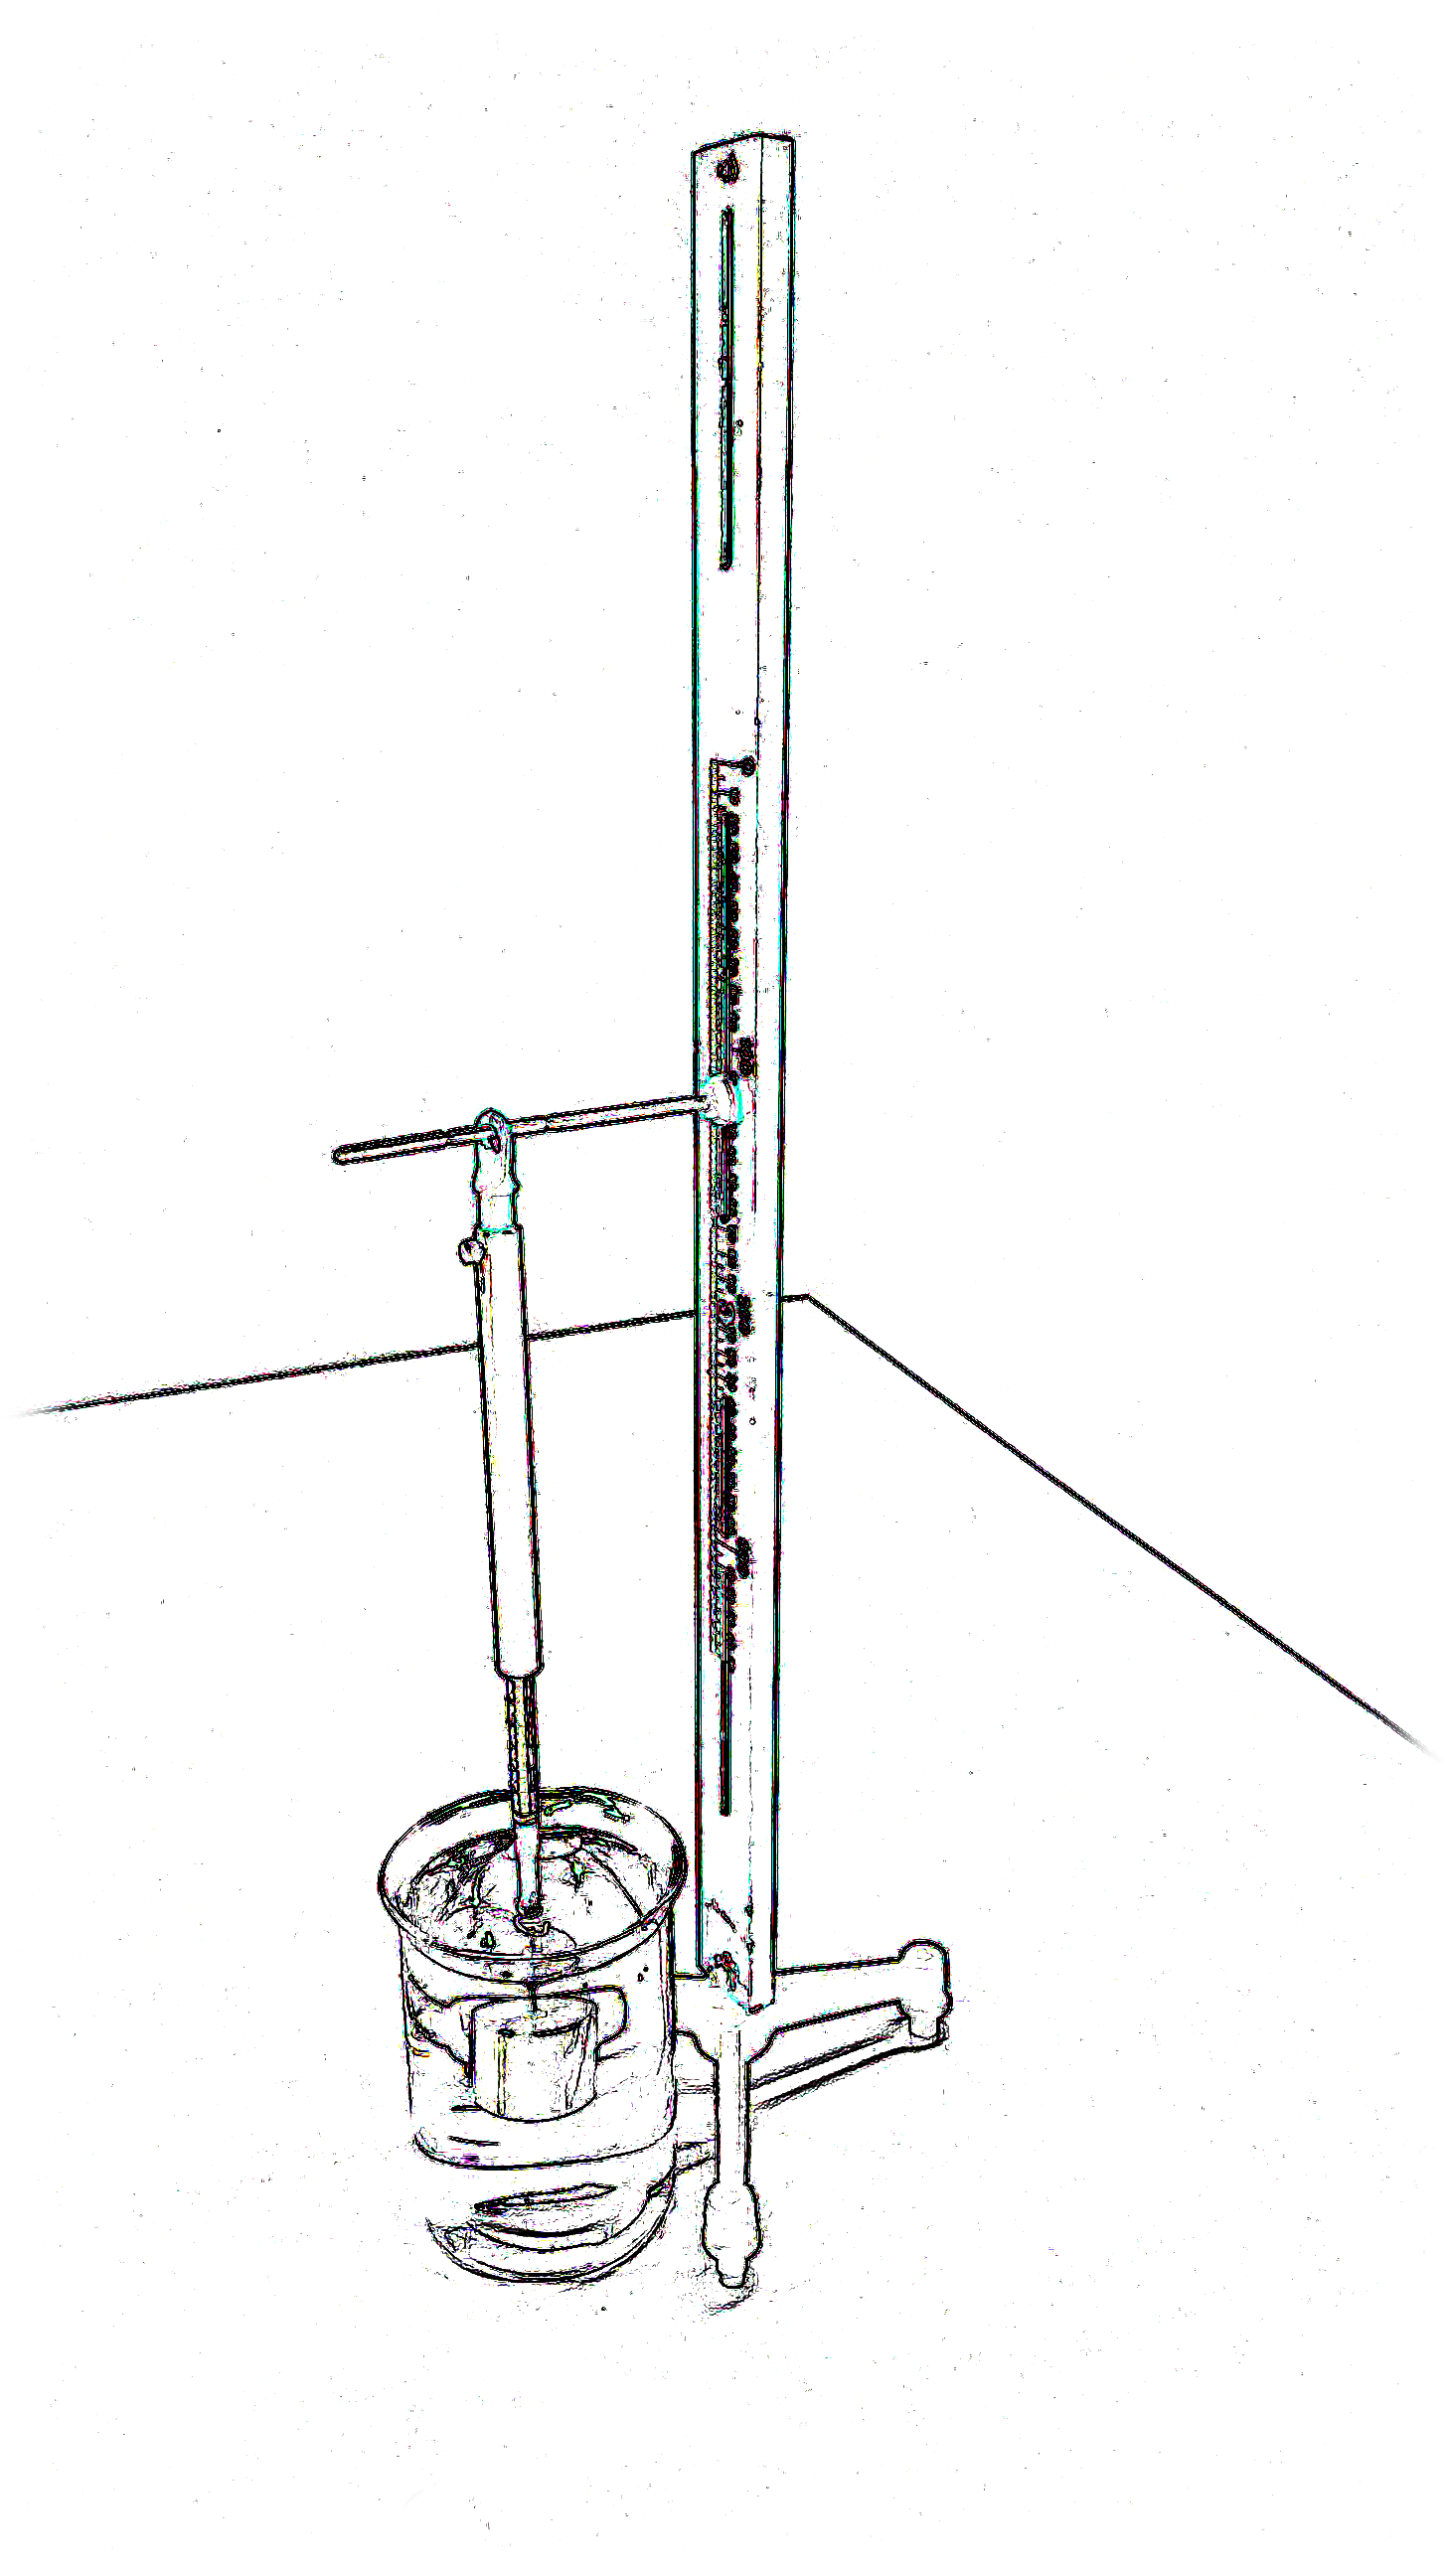
\includegraphics[width=0.7\textwidth]{Ilustrations/Empuxo.png}
\caption{Bloco metálico suspenso por um dinamômetro e submerso em água.}
\label{Fig:BeckerBloco}
\end{marginfigure}

Podemos verificar a origem dessa força se tomarmos um bloco metálico, que afunda ao ser colocado na água e o prendendo a um dinamômetro conforme mostra a Figura~\ref{Fig:BeckerBloco}. Se o becker estiver vazio, claramente a leitura do dinamômetro será igual à força peso do bloco quando o sistema estiver em equilíbrio. Se o enchermos, notaremos que o dinamômetro registrará uma nova medida de força, menor do que a primeira. O valor dessa nova medida é conhecido como \emph{peso aparente} do corpo.

\begin{marginfigure}
\centering
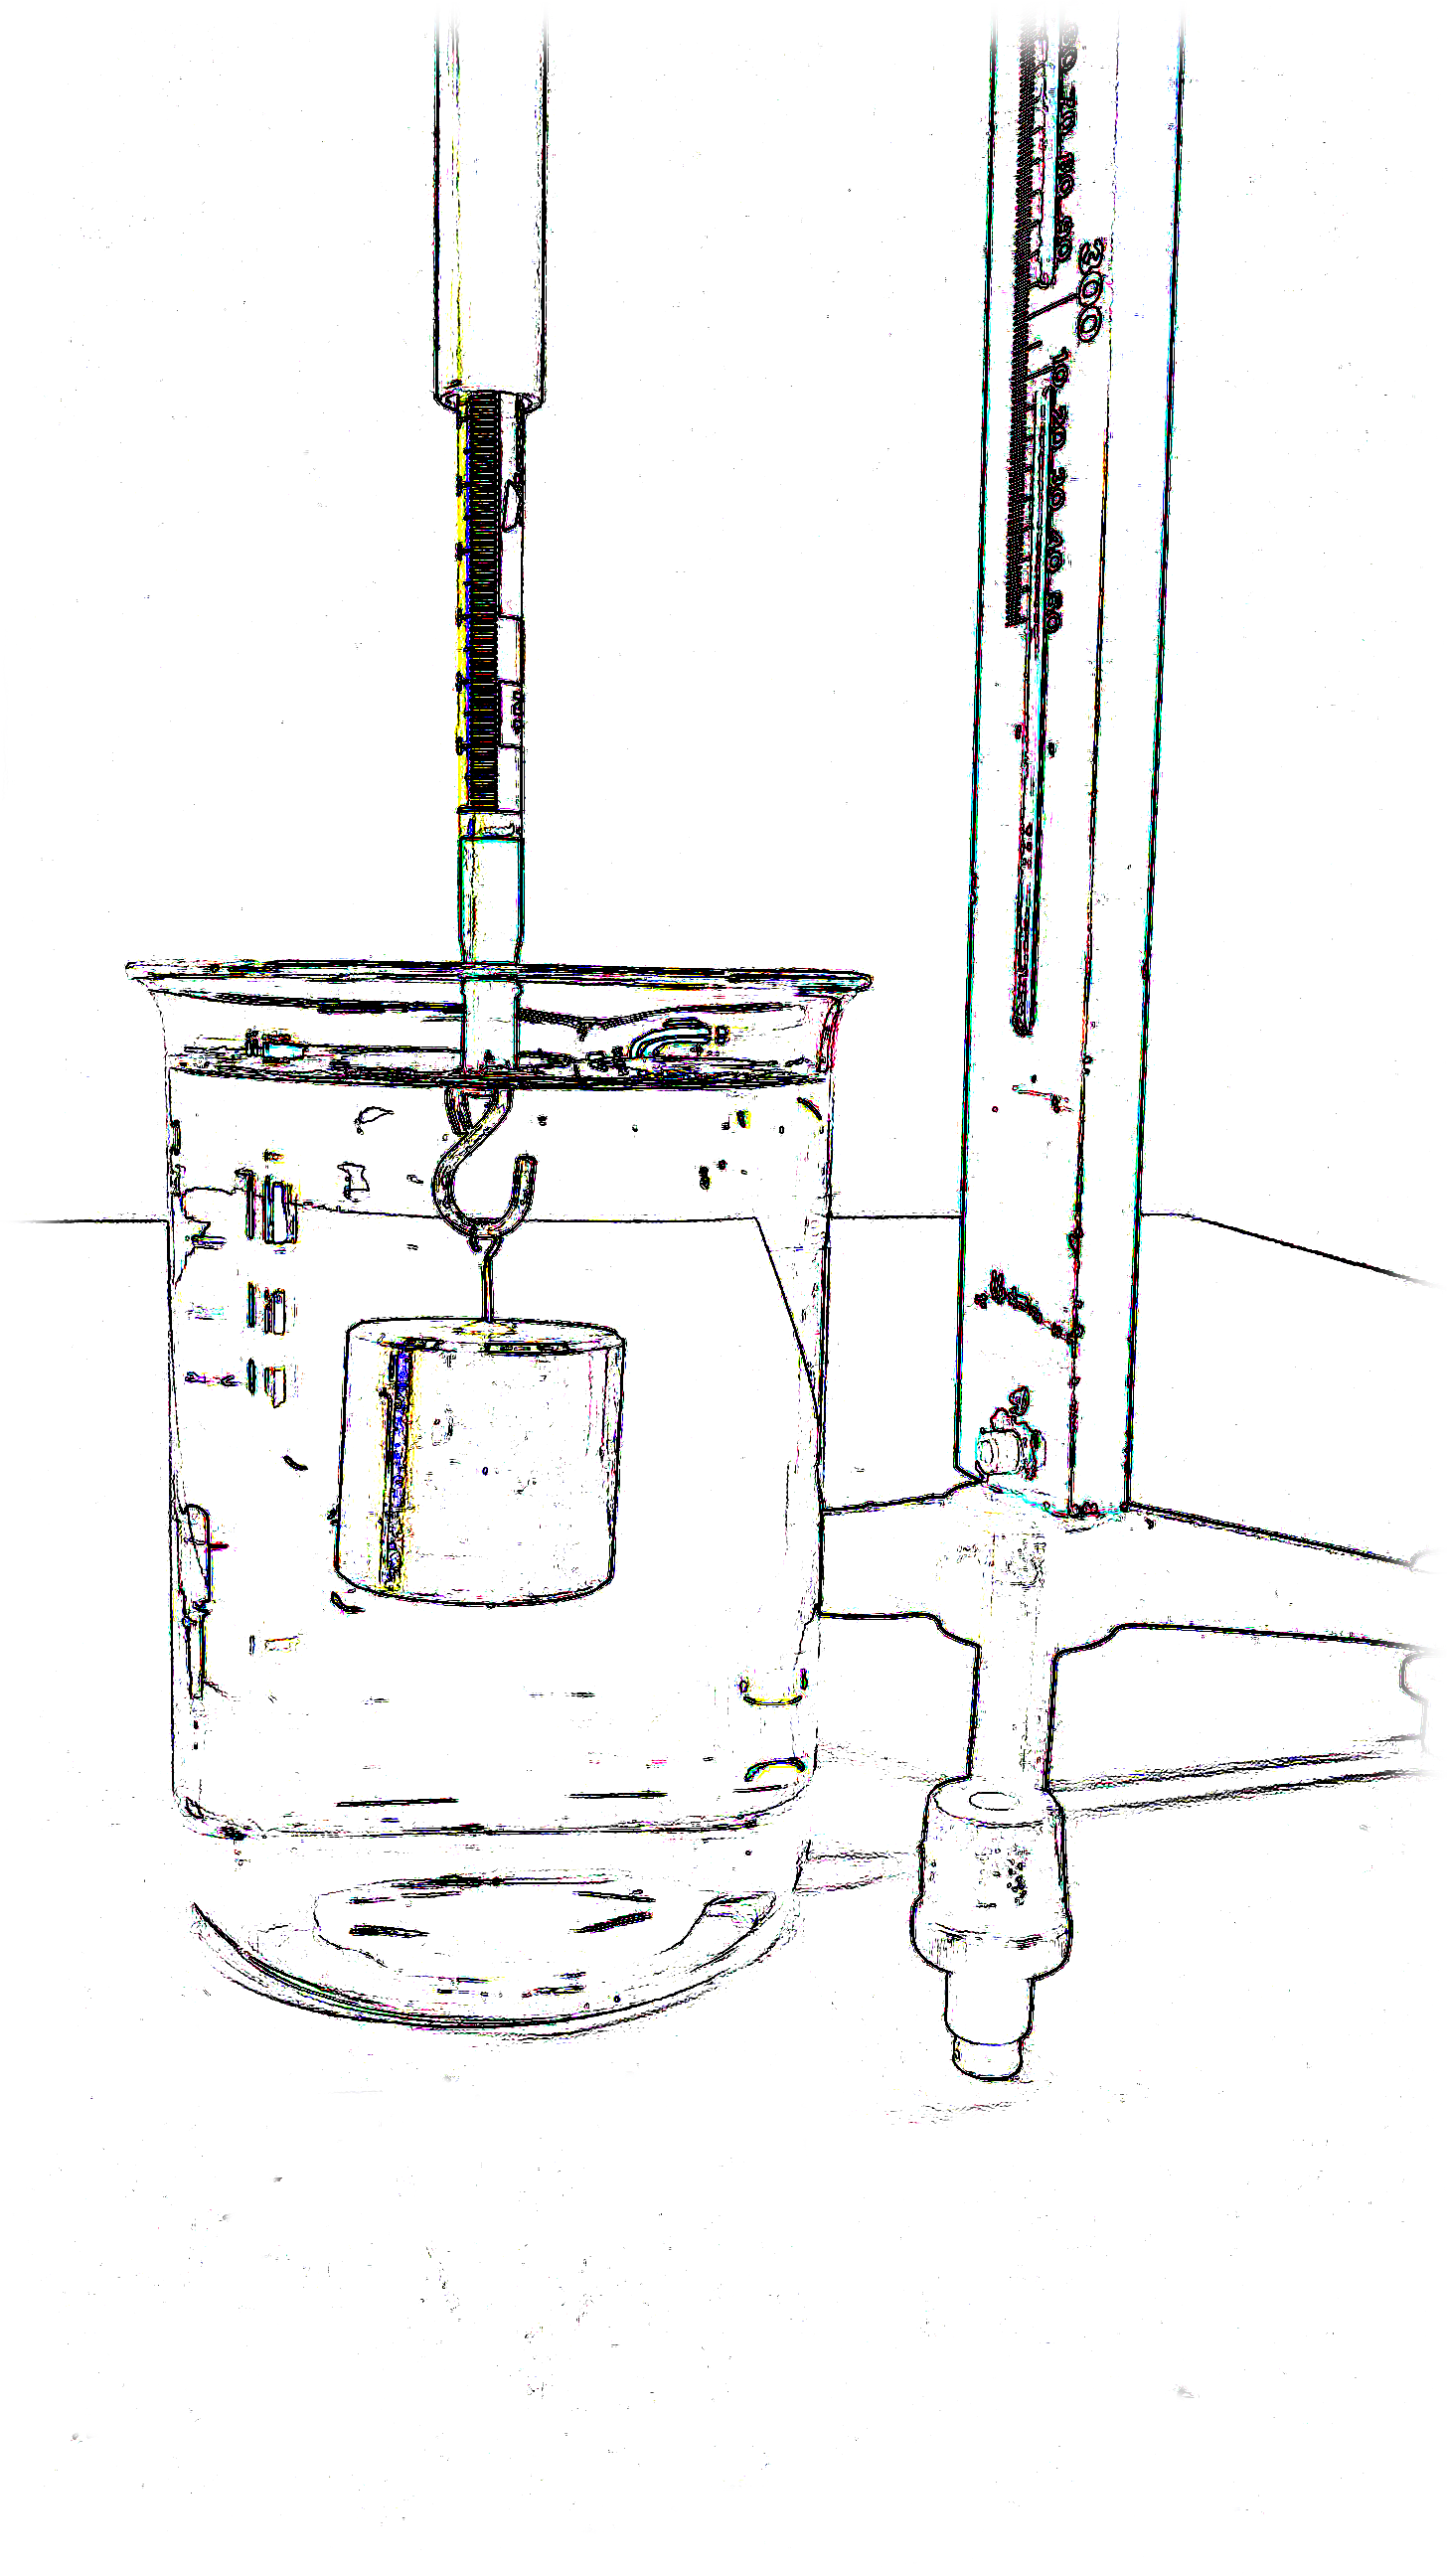
\includegraphics[width=0.5\textwidth]{Ilustrations/Empuxo_detalhe.png}
\caption{Detalhe da Figura~\ref{Fig:BeckerBloco}.}
\label{Fig:BeckerBlocoDetalhe}
\end{marginfigure}
A origem dessa diferença pode ser entendida ao analisarmos as forças exercidas pela pressão do fluido nas superfícies superior e inferior do bloco (as laterais se cancelam, veja a Figura~\ref{Fig:EmpuxoDiagramaForcas}). A pressão exercida por um fluido não é constante, aumentando conforme a profundidade aumenta, e é definida como
\begin{equation}
	P = \frac{F}{A},
\end{equation}
%
o que implica em
\begin{equation}
    F = PA.
\end{equation}
%
Logo, a força na parte inferior do bloco é maior que na parte superior, já que as áreas superior e inferior são idênticas. 
\begin{marginfigure}[1cm]
	\centering
	\begin{tikzpicture}[>=Stealth]
		\draw[pattern = north west lines] (0,0) rectangle (1,1);
		\foreach \x in {0,0.333,0.666,1}{
			\draw[->] (\x,-0.75) -- (\x,0);
			\draw[->] (\x,1.25) -- (\x,1);
		}
		\draw[->] (-0.25,1) -- (0,1);
		\draw[->] (-0.375,0.6666) -- (0,0.66666);
		\draw[->] (-0.5625,0.3333) -- (0,0.3333);
		\draw[->] (-0.75,0) -- (0,0);
		\draw[->] (1.25,1) -- (1,1);
		\draw[->] (1.4375,0.6666) -- (1,0.6666);
		\draw[->] (1.625,0.3333) -- (1,0.3333);
		\draw[->] (1.75,0) -- (1,0);
	\end{tikzpicture}
	\caption{Forças atuando nas faces de um bloco submerso. \label{Fig:EmpuxoDiagramaForcas}}
\end{marginfigure}

Essa diferença entre as forças é o que denominamos como \emph{força de empuxo}, representada aqui como $\vec{F}_E$ (Figura~\ref{Fig:BlocoBeckerDiagrama}). Sua direção e sentido são verticalmente para cima, pois equilibra --- ao menos parcialmente --- o peso. Podemos verificar a intensidade do empuxo  imaginando a seguinte situação: substituímos o volume ocupado pelo bloco por água (veja a Figura~\ref{Fig:BlAguaBeckerDiagrama}). Nesse caso, sabemos que o ``bloco de água'' deve permanecer em equilíbrio, como qualquer outra região do líquido. Se o ``bloco'' está em equilíbrio, seu peso está sendo equilibrado pelo empuxo. Logo, \emph{o empuxo tem o mesmo módulo que o peso do líquido deslocado}\footnote{Este resultado é conhecido como \emph{princípio de Arquimedes}.}. No caso do bloco metálico acima, o empuxo é equivalente ao peso de um ``bloco de água'' com o mesmo volume que o bloco metálico.

\begin{marginfigure}
\centering
\begin{tikzpicture}[>=Stealth]
	\draw[color=gray] (-1,-1) rectangle (2,2);
	\draw (0,0) rectangle (1,1);
	\foreach \x in {0,0.333,0.666,1}{
			\draw[->] (\x,-0.75) -- (\x,0);
			\draw[->] (\x,1.25) -- (\x,1);
	}
	\draw (1,1.125) node[anchor=west]{$\vec{F}_{\textrm{sup}}$};
	\draw (1,-0.675) node[anchor=west]{$\vec{F}_{\textrm{inf}}$};
	\draw[->] (0.5,0.5) -- node[above right] {$\vec{P}$} (0.5,-0.5);
	\draw[fill] (0.5,0.5) circle (0.02);	

	\draw[->] (2.5,0.5) -- (2.5,1.25) node[anchor=west]{$\vec{F}_{\textrm{inf}}$};
	\draw[->] (2.5,0.5) -- (2.5,0.25) node[anchor=west]{$\vec{F}_{\textrm{sup}}$};
	\draw[->] (2.5,0.5) -- (2.5,-0.5) node[anchor=west] {$\vec{P}$};
	\draw[fill] (2.5,0.5) circle (0.02);
	
	\draw[fill] (3.5,0.5) circle (0.02);
	\draw[->] (3.5,0.5) -- (3.5,-0.5) node[anchor=west] {$\vec{P}$};
	\draw[->] (3.5,0.5) -- (3.5,1) node[anchor=west]{$\vec{F}_{e}$};
\end{tikzpicture}
\caption{Diagrama de corpo livre representando as forças que atuam sobre o bloco quando submerso. No diagrama à direita, substituímos a soma $\vec{F}_{\textrm{inf}} + \vec{F}_{\textrm{sup}}$ das forças que atuam na parte inferior e superior do bloco por $F_e$, isto é, o empuxo. As forças laterais não estão representadas pois, por simetria, se equilibram.}
\label{Fig:BlocoBeckerDiagrama}
\end{marginfigure}

\begin{marginfigure}
\centering
\begin{tikzpicture}[>=Stealth]
	\draw[color=gray] (-1,-1) rectangle (2,2);
	\draw[dashed] (0,0) rectangle (1,1);
	\foreach \x in {0,0.333,0.666,1}{
			\draw[->] (\x,-0.75) -- (\x,0);
			\draw[->] (\x,1.25) -- (\x,1);
	}
	\draw (1,1.125) node[anchor=west]{$\vec{F}_{\textrm{sup}}$};
	\draw (1,-0.675) node[anchor=west]{$\vec{F}_{\textrm{inf}}$};
	\draw[->] (0.5,0.5) -- node[right] {$\vec{P}$} (0.5,0);
	\draw[fill] (0.5,0.5) circle (0.02);	

	\draw[->] (2.5,0.5) -- (2.5,1.25) node[anchor=west]{$\vec{F}_{\textrm{inf}}$};
	\draw[->] (2.5,0.5) -- (2.5,0.25) node[anchor=west]{$\vec{F}_{\textrm{sup}}$};
	\draw[->] (2.5,0.5) -- (2.5,0) node[anchor=east] {$\vec{P}$};
	\draw[fill] (2.5,0.5) circle (0.02);
	
	\draw[fill] (3.5,0.5) circle (0.02);
	\draw[->] (3.5,0.5) -- (3.5,0) node[anchor=west] {$\vec{P}$};
	\draw[->] (3.5,0.5) -- (3.5,1) node[anchor=west]{$\vec{F}_{e}$};
\end{tikzpicture}
\caption{Diagrama de corpo livre representando as forças que atuam sobre uma massa de água que ocupa o volume original do bloco. As forças devido à pressão são iguais ao caso do bloco, porém o peso é menor. Como o meio é todo composto por água e deve então estar em equilíbrio, concluímos que o empuxo deve ser igual ao peso do volume de água deslocado (caso contrário não haveria equilíbrio).}
\label{Fig:BlAguaBeckerDiagrama}
\end{marginfigure}
%%%%%%%%%%%%%%%%%%%%%%%%%%%%%%%%%%%%%%%%%%%%%%%%%%%%%%%%%%%%%%%%%%%%%%%%%%%%%%%
\section{Cálculo de densidades}
%%%%%%%%%%%%%%%%%%%%%%%%%%%%%%%%%%%%%%%%%%%%%%%%%%%%%%%%%%%%%%%%%%%%%%%%%%%%%%%

%%%%%%%%%%%%%%%%%%%%%%%%%%%%%%%%%%%
\subsection{Densidade de um sólido}
%%%%%%%%%%%%%%%%%%%%%%%%%%%%%%%%%%%

Podemos calcular a razão da densidade de um objeto pela densidade da água usando um dinamômetro e uma proveta. Se pendurarmos o objeto no dinamômetro, verificaremos que --- no equilíbrio --- ele nos dará a leitura do módulo da força peso do objeto. Quando o mergulhamos, no entanto, teremos uma leitura menor, que denominamos anteriormente como peso aparente.

Temos então que
\begin{align}
	P &= \rho Vg \\
	F_E &= \rho_{\textrm{água}} V g
\end{align}
%
onde $F_E$ é igual ao peso do volume de água deslocado, $\rho$ é a densidade do material e $\rho_{\textrm{água}}$ é a densidade da água. Calculando a razão entre as equações acima, temos
\begin{equation}
	\frac{P}{F_E} = \frac{\rho Vg}{\rho_{\textrm{água}}Vg} = \frac{\rho}{\rho_{\textrm{água}}},
\end{equation}
%
de onde podemos escrever, lembrando que o peso aparente é dado por
\begin{equation}
	P_{\textrm{ap}} = P - F_E,
\end{equation}
%
a seguinte relação para a razão $\rho/\rho_{\textrm{água}}$:
\begin{equation}\label{Eq:DensRelativa}
	\frac{\rho}{\rho_{\textrm{água}}} = \frac{P}{P-P_{\textrm{ap}}}.
\end{equation}

%%%%%%%%%%%%%%%%%%%%%%%%%%%%%%%%%%%
\subsection{Densidade de um fluido}
%%%%%%%%%%%%%%%%%%%%%%%%%%%%%%%%%%%

Podemos utilizar uma proveta, um fluido, uma balança, e um conjunto de corpos de prova para verificar a densidade do fluido.


\begin{marginfigure}
\centering
\begin{tikzpicture}[>=Stealth,
     interface/.style={
        % superfície
        postaction={draw,decorate,decoration={border,angle=-45,
                    amplitude=0.2cm,segment length=2mm}}},
    ]

    \draw[interface] (-2,0) -- (2,0);
    
    \draw[pattern = north west lines] (-1.5,3) -- (-1.5,0) -- (1.5,0) -- (1.5,3) -- (1.3,3) -- (1.3,0.2) -- (-1.3, 0.2) -- (-1.3,3) -- cycle;
    
    %\draw[pattern = dots] (-1.3,2.5) -- (0,2.5) -- (0,2) -- (-0.5,2) -- (-0.5, 1) -- (0.5,1) -- (0.5,2) -- (0,2) -- (0,2.5) -- (1.3,2.5) -- (1.3,0.2) -- (-1.3,0.2) -- cycle;
    
    \draw[dashed] (-1.3, 2.75) -- (1.3, 2.75);
        
    \draw (0,2) -- (0,4);
    \draw[->, thick] (0,2) -- (0,3.25) node[right]{$\vec{T}$};
    \draw[pattern = north west lines] (-0.5,1) rectangle (0.5,2);
    
    \draw[->, thick] (-0.25,2) -- +(0,0.5) node[left]{$\vec{E}$};
    \draw[<-, thick] (-0.25,0.2) -- node[left]{$\vec{E}'$} +(0,0.5);
    
\end{tikzpicture}
\caption{A reação à força de empuxo exercida sobre o corpo atua sobre o fundo do recipiente.\label{Fig:ReacaoEmpuxo}}
\end{marginfigure}

Se tomarmos a proveta e a preenchermos com água até um certo nível, podemos pesá-la e encontraremos um valor para a massa do sistema. Ao pendurarmos o corpo de prova de forma que ele \emph{esteja submerso, porém sem tocar as laterais da proveta ou seu fundo}, verificaremos um aumento na leitura da balança, porém esse aumento \emph{não corresponderá à massa do corpo}. Ao verificarmos o diagrama de forças das Figuras~\ref{Fig:BlocoBeckerDiagrama} e~\ref{Fig:BlAguaBeckerDiagrama}, vemos que ao mergulharmos o corpo, há uma força de empuxo $\vec{E}$ dirigida para cima e que equilibra parcialmente o peso do objeto. Onde está a reação a esta força de empuxo? A reação a esta força deve agir sobre o líquido, que --- por sua vez --- exerce força sobre as paredes do recipiente (Figura~\ref{Fig:ReacaoEmpuxo}). Como as forças exercidas sobre uma lateral qualquer se equilibram com as forças exercidas sobre a lateral oposta, resta a força exercida sobre o fundo do recipiente. Nessa situação, temos então que a balança registrará uma ``massa aparente'' adicional dada por\footnote{Mesmo em uma balança de braços, o que a balança registra é a força normal exercida para equilibrar o objeto, apesar de a escala estar marcada em unidades de massa.}
\begin{equation}
	m_{\textrm{ap}} = \frac{F_E}{g}.
\end{equation}
%
Como o empuxo é o peso do volume de água deslocado, temos
\begin{align}
	m_{\textrm{ap}} &= \frac{m_{\textrm{água}}g}{g} \\
	&=m_{\textrm{água}}.
\end{align}
%
Podemos então calcular a densidade da água através da razão entre a diferença das massas (depois e antes da submersão do corpo) e a diferença dos volumes indicados pela proveta:\footnote{As variáveis $m'$ e $V'$ denotam os valores registrados pela balança e pela proveta após a submersão do corpo.}
\begin{equation}
	\rho_{\textrm{água}} = \frac{m'-m}{V'-V}.
\end{equation}

Note que se tomarmos um gráfico dos valores de $m'\times V'$ para diversos corpos submersos, temos que a inclinação do gráfico será dada por
\begin{equation}
    B = \frac{\Delta m}{\Delta V}.
\end{equation}
%
Assim, se fizermos um gráfico desse tipo e traçarmos a melhor reta, podemos obter $\rho_{\text{água}}$ através do coeficiente angular. 


%%%%%%%%%%%%%%%%%%%%%%%%%%%%%%%%%%%%%%%%%%%%%%%%%%%%%%%%%%%%%%%%%%%%%%%%%%%%%%%
\section{Experimento}
%%%%%%%%%%%%%%%%%%%%%%%%%%%%%%%%%%%%%%%%%%%%%%%%%%%%%%%%%%%%%%%%%%%%%%%%%%%%%%%

%%%%%%%%%%%%%%%%%%%%%%
\subsection{Objetivos}
\label{Sec:ObjetivosEmpuxo}
%%%%%%%%%%%%%%%%%%%%%%

\begin{enumerate}
	\item Verificar experimentalmente a existência da força de empuxo e a existência de um peso aparente para um objeto submerso.
	\item Verificar experimentalmente a densidade de corpos de prova utilizando um dinamômetro e uma proveta.
	\item Verificar experimentalmente a reação ao empuxo.
	\item Verificar experimentalmente a densidade de um líquido utilizando uma balança e uma proveta.
\end{enumerate}

%%%%%%%%%%%%%%%%%%%%%%%%%%%%%%%%%%%%%%%%%%%%%%%%%%%%%%%%%%%%%%%%%%%%%%%%%%%%%%%
\section{Material Necessário}
%%%%%%%%%%%%%%%%%%%%%%%%%%%%%%%%%%%%%%%%%%%%%%%%%%%%%%%%%%%%%%%%%%%%%%%%%%%%%%%

\begin{itemize}
	\item Proveta;
	\item Balança;
	\item Dinamômetro;
	\item Becker com água;
	\item Corpos de prova diversos;
	\item Suporte vertical com haste horizontal.
\end{itemize}

%%%%%%%%%%%%%%%%%%%%%%%%%%%%%%%%%%%%%%%%%%%%%%%%%%%%%%%%%%%%%%%%%%%%%%%%%%%%%%%
\section{Procedimento Experimental}
%%%%%%%%%%%%%%%%%%%%%%%%%%%%%%%%%%%%%%%%%%%%%%%%%%%%%%%%%%%%%%%%%%%%%%%%%%%%%%%

%%%%%%%%%%%%%%%%%%%%%%%%%%%%%%%%%%%%%%%%%%%%%%%%%%%
\subsection{Determinação da densidade de um sólido}
%%%%%%%%%%%%%%%%%%%%%%%%%%%%%%%%%%%%%%%%%%%%%%%%%%%
\begin{enumerate}
	\item Disponha o dinamômetro na vertical com o auxílio do suporte com haste.
	\item Zere o dinamômetro
	\item Suspenda um corpo de prova usando o gancho do dinamômetro e efetue a leitura do peso real.
	\item Mergulhe o corpo de prova de forma que ele não toque nas paredes e no fundo do becker. Verifique o valor do peso aparente.
	\item Anote os dados obtidos para o peso na Tabela~\ref{Tab:DadosEmpuxo}
	\item Repita os itens 3 a 5 acima para os demais corpos de prova.
\end{enumerate}

%%%%%%%%%%%%%%%%%%%%%%%%%%%%%%%%%%%%%%%%%%%%%%%%%
\subsection{Determinação da densidade da água}
%%%%%%%%%%%%%%%%%%%%%%%%%%%%%%%%%%%%%%%%%%%%%%%%%
\begin{enumerate}
\item Coloque \np[ml]{150,0} na proveta e meça a massa da proveta com a água;
\item Mergulhe o corpo de prova na proveta, cuidando para que ele não toque no fundo e nas bordas da proveta e determine a massa do conjunto;
\item Obtenha também a leitura para o volume indicado pela proveta.
\item Repita os itens 2 e 3 para os demais corpos.
\item Anote os resultados na Tabela~\ref{Tab:DadosEmpuxo}
\end{enumerate}

%%%%%%%%%%%%%%%%%%%%%%%%%%%%%%%%%%%%%%%%%%%%%%%%%%%%%%%%%%%%%%%%%%%%%%%%%%%%%%%
%%%%%%%%%%%%%%%%%%%%%%%%%%%%%%%%%%%%%%%%%%%%%%%%%%%%%%%%%%%%%%%%%%%%%%%%%%%%%%%
%%%%%%%%%%%%%%%%%%%%%%%%%%%%%%%%%%%%%%%%%%%%%%%%%%%%%%%%%%%%%%%%%%%%%%%%%%%%%%%
%%%%%%%%%%%%%%%%%%%%%%%%%%%%%%%%%%%%%%%%%%%%%%%%%%%%%%%%%%%%%%%%%%%%%%%%%%%%%%%
\cleardoublepage

\noindent{}{\huge\textit{Empuxo}}

\vspace{15mm}

\begin{fullwidth}
\noindent{}\makebox[0.6\linewidth]{Turma:\enspace\hrulefill}\makebox[0.4\textwidth]{  Data:\enspace\hrulefill}
\vspace{5mm}

\noindent{}\makebox[0.6\linewidth]{Aluno(a):\enspace\hrulefill}\makebox[0.4\textwidth]{  Matrícula:\enspace\hrulefill}

\noindent{}\makebox[0.6\linewidth]{Aluno(a):\enspace\hrulefill}\makebox[0.4\textwidth]{  Matrícula:\enspace\hrulefill}

\noindent{}\makebox[0.6\linewidth]{Aluno(a):\enspace\hrulefill}\makebox[0.4\textwidth]{  Matrícula:\enspace\hrulefill}

\noindent{}\makebox[0.6\linewidth]{Aluno(a):\enspace\hrulefill}\makebox[0.4\textwidth]{  Matrícula:\enspace\hrulefill}

\noindent{}\makebox[0.6\linewidth]{Aluno(a):\enspace\hrulefill}\makebox[0.4\textwidth]{  Matrícula:\enspace\hrulefill}
\end{fullwidth}

\vspace{5mm}

%%%%%%%%%%%%%%%%%%%%%%%%%%%%%%%%%%%%%%%%%%%%%%%%%%%%%%%%%%%%%%%%%%%%%%%%%%%%%%%
\section{Questionário}
%%%%%%%%%%%%%%%%%%%%%%%%%%%%%%%%%%%%%%%%%%%%%%%%%%%%%%%%%%%%%%%%%%%%%%%%%%%%%%%

\begin{question}[type={exam}]{1}
Apresente os resultados de maneira clara e organizada. Mostre os cálculos requisitados de maneira clara e sucinta, evidenciando o raciocínio desenvolvido.
\end{question}

\begin{question}[type={exam}]{1}
Liste os equipamentos utilizados. Para os instrumentos de medida, descreva o tipo do equipamento, sua resolução, e seu erro de escala.
\end{question}

\begin{question}[type={exam}]{1}
Preencha as tabelas com o número adequado de algarismos significativos, unidades, e erros de escala apropriados. 
\end{question}

\begin{question}[type={exam}]{1}
Elabore um gráfico de $m' \times V'$ para os dados da Tabela~\ref{Tab:DadosEmpuxo}.
\end{question}

\begin{question}[type={exam}]{1.5}
Calcule a reta que melhor representa os dados experimentais na questão acima utilizando o método dos mínimos quadrados e a adicione ao gráfico.
\end{question}

\begin{question}[type={exam}]{1.5}
Calcule os valores para a densidade relativa $(\rho/\rho_{\textrm{água}})$ dos sólidos, juntamente com o erro propagado, através da Equação~\ref{Eq:DensRelativa}. Apresente os cálculos e preencha com os resultados obtidos a coluna correspondente da Tabela~\ref{Tab:DadosEmpuxo}. 
\end{question}

\begin{question}[type={exam}]{1.5}
Deduza a equação para o erro em uma divisão
\begin{equation}
    (q \pm \delta q) = (x \pm \delta x) \div (y \pm \delta y)
\end{equation}
%
a partir da Equação~\eqref{Eq:ErroGeral}.
\end{question}

\begin{question}[type={exam}]{1.5}
Considerando os objetivos do experimento, listados na Seção~\ref{Sec:ObjetivosEmpuxo}, e os resultados obtidos nas questões anteriores, discuta quais objetivos foram atingidos com sucesso, justificando suas conclusões. Se algum objetivo não foi atingido, discuta quais são os possíveis motivos do fracasso e que providências podem ser tomadas para que eles sejam alcançados.
\end{question}

\vfill
%%%%%%%%%%%%%%%%%%%%%%%%%%%%%%%%%%%%%%%%%%%%%%%%%%%%%%%%%%%%%%%%%%%%%%%%%%%%%%%
\pagebreak
\section{Tabelas}
%%%%%%%%%%%%%%%%%%%%%%%%%%%%%%%%%%%%%%%%%%%%%%%%%%%%%%%%%%%%%%%%%%%%%%%%%%%%%%%

\begin{table}
\label{Tab:DadosEmpuxo}
	\begin{center}
		\begin{tabular}{cp{25mm}p{25mm}p{25mm}c}
		\toprule
		&\multicolumn{3}{l}{\textbf{Dados de peso e peso aparente para os corpos de prova.}} \\
		\cmidrule{2-4}
		& $P$ & $P_{\textrm{ap}}$ & $\rho/\rho_{\textrm{água}}$ & \\
		\cmidrule{2-4}
		& \cellcolor[gray]{0.89} & \cellcolor[gray]{0.92} & \cellcolor[gray]{0.89} \\
		& \cellcolor[gray]{0.95} & \cellcolor[gray]{0.97} & \cellcolor[gray]{0.95} \\
		& \cellcolor[gray]{0.89} & \cellcolor[gray]{0.92} & \cellcolor[gray]{0.89} \\
		& \cellcolor[gray]{0.95} & \cellcolor[gray]{0.97} & \cellcolor[gray]{0.95} \\
		& \cellcolor[gray]{0.89} & \cellcolor[gray]{0.92} & \cellcolor[gray]{0.89} \\
\\
		&\multicolumn{3}{l}{\textbf{Dados a leitura de volume e massa.}} \\
		\cmidrule{2-3}
		& $V'$ & $m'$ \\
		\cmidrule{2-3}
		& \cellcolor[gray]{0.89} & \cellcolor[gray]{0.92} \\
		& \cellcolor[gray]{0.95} & \cellcolor[gray]{0.97} \\
		& \cellcolor[gray]{0.89} & \cellcolor[gray]{0.92} \\
		& \cellcolor[gray]{0.95} & \cellcolor[gray]{0.97} \\
		& \cellcolor[gray]{0.89} & \cellcolor[gray]{0.92} \\
		\cmidrule{2-3}
		\cmidrule{2-4}
		\bottomrule
		\end{tabular}
	\end{center}
	\caption{Dados para as leituras de massa, volume, peso e peso aparente.}
\end{table}
%

%%%%%%%%%%%%%%%%%%%%%%%%%%%%%%%%%%%%%%%%%%%%%%%%%%%%%%%%%%%%%%%%%%%%%%%%%%%%%%%
\chapter{Oscilações}
\label{Chap:ExpOscilacoes}
%%%%%%%%%%%%%%%%%%%%%%%%%%%%%%%%%%%%%%%%%%%%%%%%%%%%%%%%%%%%%%%%%%%%%%%%%%%%%%%

\begin{fullwidth}\it
	Verificaremos o comportamento oscilatório de dois sistemas -- um sistema massa-mola e um pêndulo simples --. Veremos que através das Leis de Newton, chegamos a uma equação cuja solução é uma função periódica que descreve o movimento oscilatório observado. Utilizaremos os seguintes conceitos/técnicas de análise de dados: medidas, algarismos significativos, gráficos, erros de escala e propagados, equação geral para o erro propagado, regressão linear, linearização, e erros dos coeficientes $A$ e $B$.
\end{fullwidth}

%%%%%%%%%%%%%%%%%%%%%%%%%%%%%%%%%%%%%%%%%%%%%%%%%%%%%%%%%%%%%%%%%%%%%%%%%%%%%%%
\section{Sistema massa-mola}
%%%%%%%%%%%%%%%%%%%%%%%%%%%%%%%%%%%%%%%%%%%%%%%%%%%%%%%%%%%%%%%%%%%%%%%%%%%%%%%

Sabemos que a força exercida por uma mola é proporcional à sua distensão:
\begin{align}
	F &= -k\Delta x \\
	&= -kx,
\end{align}
%
onde assumimos que $x_0 = 0$, $k$ é uma constante de proporcionalidade e o sinal negativo significa que a força é no sentido contrário à distensão da mola.

\begin{marginfigure}
	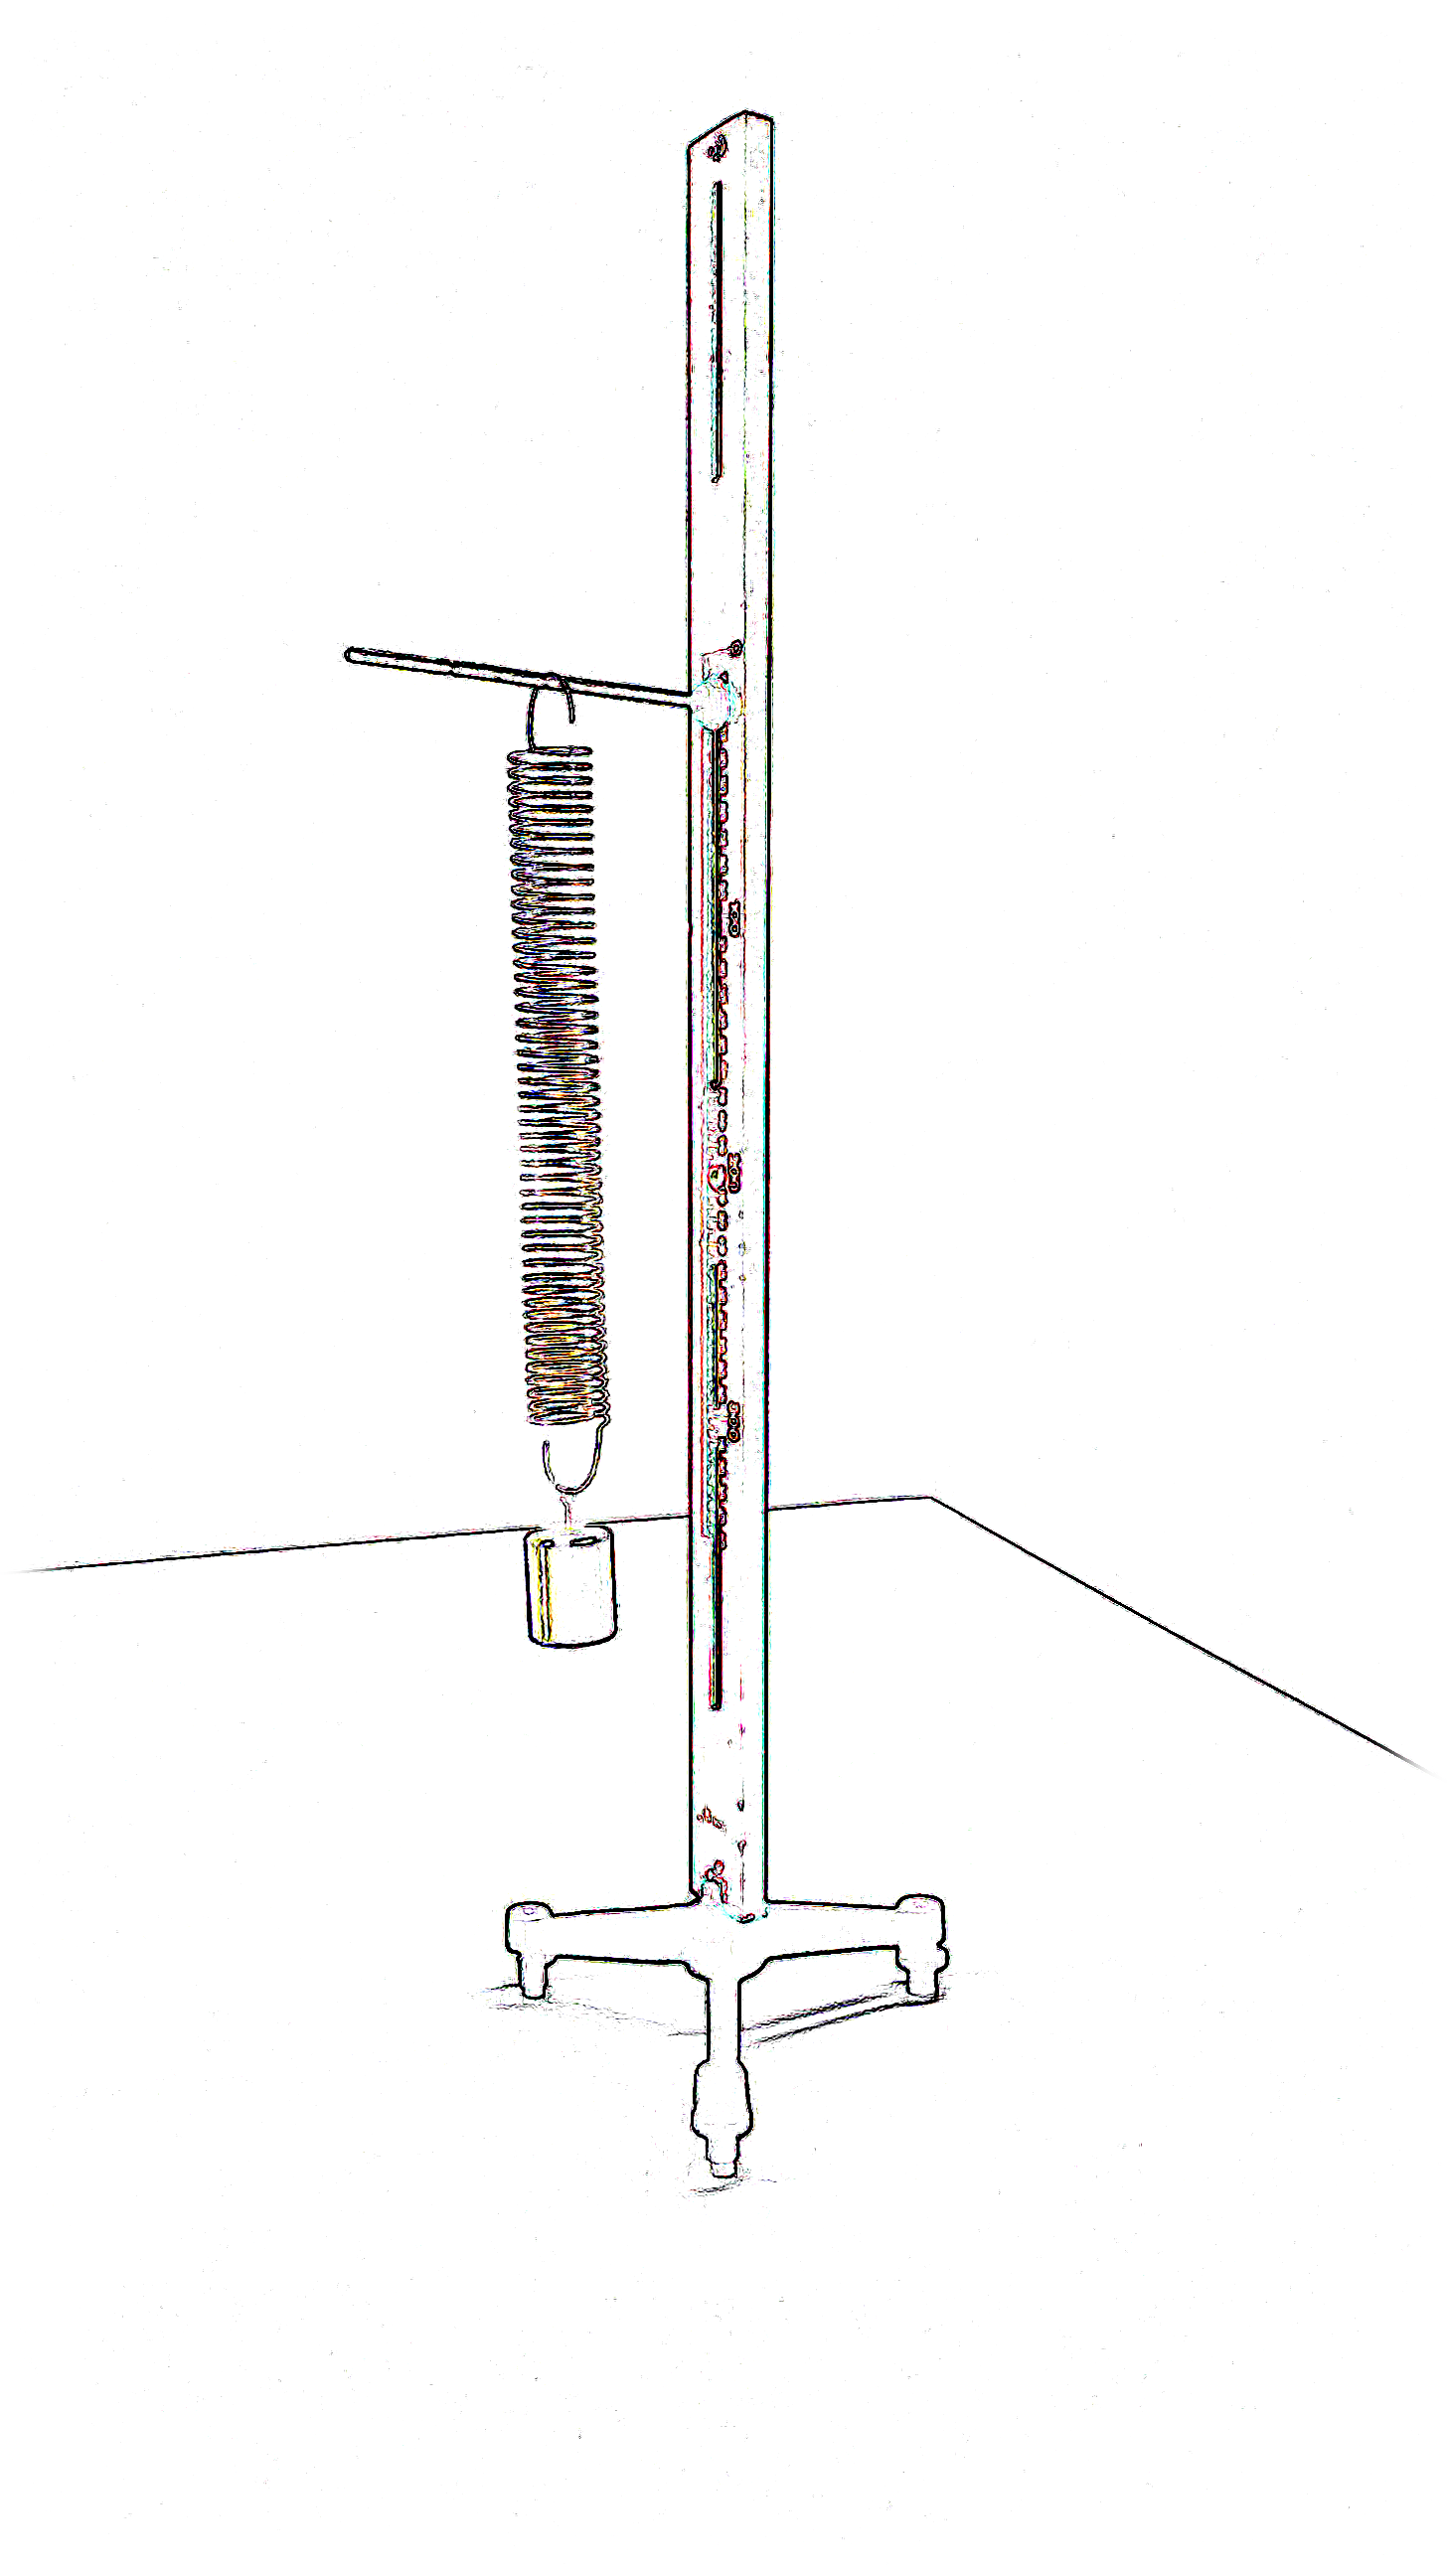
\includegraphics[width=\textwidth]{Ilustrations/Massa-Mola.png}
	\caption{Sistema massa-mola.}
\end{marginfigure}

Se pendurarmos uma mola em um suporte -- de forma que ela se disponha verticalmente -- e prendermos um corpo de massa apreciável à extremidade inferior. Deixamos o corpo descer até que a força exercida pela mola equilibre o peso. A partir dessa posição de equilíbrio, qualquer deslocamento exercido fará com que atue sobre o corpo uma força proporcional ao deslocamento, porém com sentido contrário a ele. Utilizando a segunda lei de Newton, podemos descrever a dinâmica do corpo através de
\begin{equation}
	-kx = ma.
\end{equation}
%
Analisando essa equação, temos que sempre que o corpo se desloca em relação à posição de equilíbrio, ele está sujeito a uma força contraria a esse deslocamento, acelerando-o em direção à posição de deslocamento zero (ou seja, a posição de equilíbrio). Quando o objeto passa pela posição de equilíbrio, sua aceleração é zero, porém sua velocidade não, o que o faz passar de tal posição e continuar o movimento oscilatório. Para tentar descrever esse movimento, podemos substituir a aceleração na equação acima por sua definição em termos da derivada segunda da posição em relação ao tempo:
\begin{equation}
	-kx = m\frac{d^2x}{dt^2},
\end{equation}
%
ou, rearranjando os termos,
\begin{equation}\label{Eq:EquacaoDiferencialOHS}
	\frac{d^2x}{dt^2} + \frac{k}{m} x = 0.
\end{equation}

Através da equação acima, percebemos que a posição $x$ como função do tempo satisfaz uma condição curiosa: a posição vezes uma constante mais sua derivada segunda é zero, ou seja, a função $x(t)$ é tal que sua derivada é igual a ela mesma, vezes uma contante. Existem duas funções que satisfazem essa condição: as funções trigonométricas $\sen$ e $\cos$. Se supusermos que $x(t)$ é então da forma
\begin{equation}
	x(t) = A\sen(\omega t)
\end{equation}
%
e a substituirmos na Equação~\eqref{Eq:EquacaoDiferencialOHS}, temos
\begin{equation}
	-A\omega^2\sen(\omega t) + \frac{k}{m}A\sen(\omega t)=0
\end{equation}
%
o que pode ser simplificado a
\begin{equation}
	\omega^2 = \frac{k}{m}.
\end{equation}

%\begin{marginfigure}
%\centering
%\includegraphics[width=5cm]{Fig/MassaMolaCaneta.png}
%\caption{Sistema massa-mola em que uma caneta foi afixada à massa, riscando sobre uma folha de papel que se move para a esquerda com velocidade constante. Podemos ver que a curva que se forma é uma senoide.}
%\end{marginfigure}

Verificamos então que a forma suposta para $x(t)$ é solução da Equação~\eqref{Eq:EquacaoDiferencialOHS} se $\omega = \sqrt{k/m}$. Portanto, concluímos que a posição do objeto descreve uma curva senoidal em um gráfico da posição em função do tempo. A partir da expressão para a posição, podemos calcular a velocidade e a aceleração em função do tempo
\begin{align}
	v(t) &= A\omega\cos\omega t \\
	a(t) &= -A\omega^2\sen\omega t.
\end{align}

Se analisarmos a função seno, vemos que ela tem um período igual a $2\pi$, isto é, seu gráfico se repete a cada $2\pi$ radianos. Isso se reflete em um ciclo de oscilação do sistema massa mola, pois após o argumento do seno atingir $2\pi$, o movimento se repete. Se considerarmos que o tempo para completar uma oscilação é o período $T$, temos, no instante que o objeto termina uma oscilação
\begin{equation}
	\omega T = 2\pi
\end{equation}
%
o que leva à seguinte equação para o período:
\begin{equation}
	T = 2\pi \frac{1}{\omega}.
\end{equation}
%
Substituindo a expressão para $\omega$, temos
\begin{equation}
	T = 2\pi \sqrt{\frac{m}{k}}.
\end{equation}
%
Verificamos então que o período de oscilação do sistema massa-mola depende da massa do objeto e da constante $k$ da mola.

Expressões como a Equação~\eqref{Eq:EquacaoDiferencialOHS} são comuns em física e são denominadas \emph{Equações Diferenciais Ordinárias}. As soluções para estas equações são \emph{funções}. A Equação~\eqref{Eq:EquacaoDiferencialOHS} em particular define o \emph{Movimento Harmônico Simples}.

%%%%%%%%%%%%%%%%%%%%%%%%%%%%%%%%%%%%%%%%%%%%%%%%%%%%%%%%%%%%%%%%%%%%%%%%%%%%%%%
\section{Pêndulo Simples}
%%%%%%%%%%%%%%%%%%%%%%%%%%%%%%%%%%%%%%%%%%%%%%%%%%%%%%%%%%%%%%%%%%%%%%%%%%%%%%%

Podemos tratar um objeto que oscila preso a uma corda de massa desprezível como uma oscilação harmônica desde que o ângulo máximo de oscilação -- isto é, a amplitude -- seja pequena. Se essa condição for garantida, o pêndulo é denominado \emph{pêndulo simples}.

Se deslocarmos um pêndulo para a direita, como na Figura~\ref{Fig:Pendulo}, teremos uma componente da força peso que tende a restaurar o pêndulo à posição de equilíbrio. Podemos ver que tal componente tem valor $P_t=P\sen\theta$, onde $P=mg$ representa o peso. De acordo com a segunda lei de Newton, temos então
\begin{equation}
	-mg\sen\theta = ma,
\end{equation}
\begin{marginfigure}
	\centering
%	\forcerectofloat
	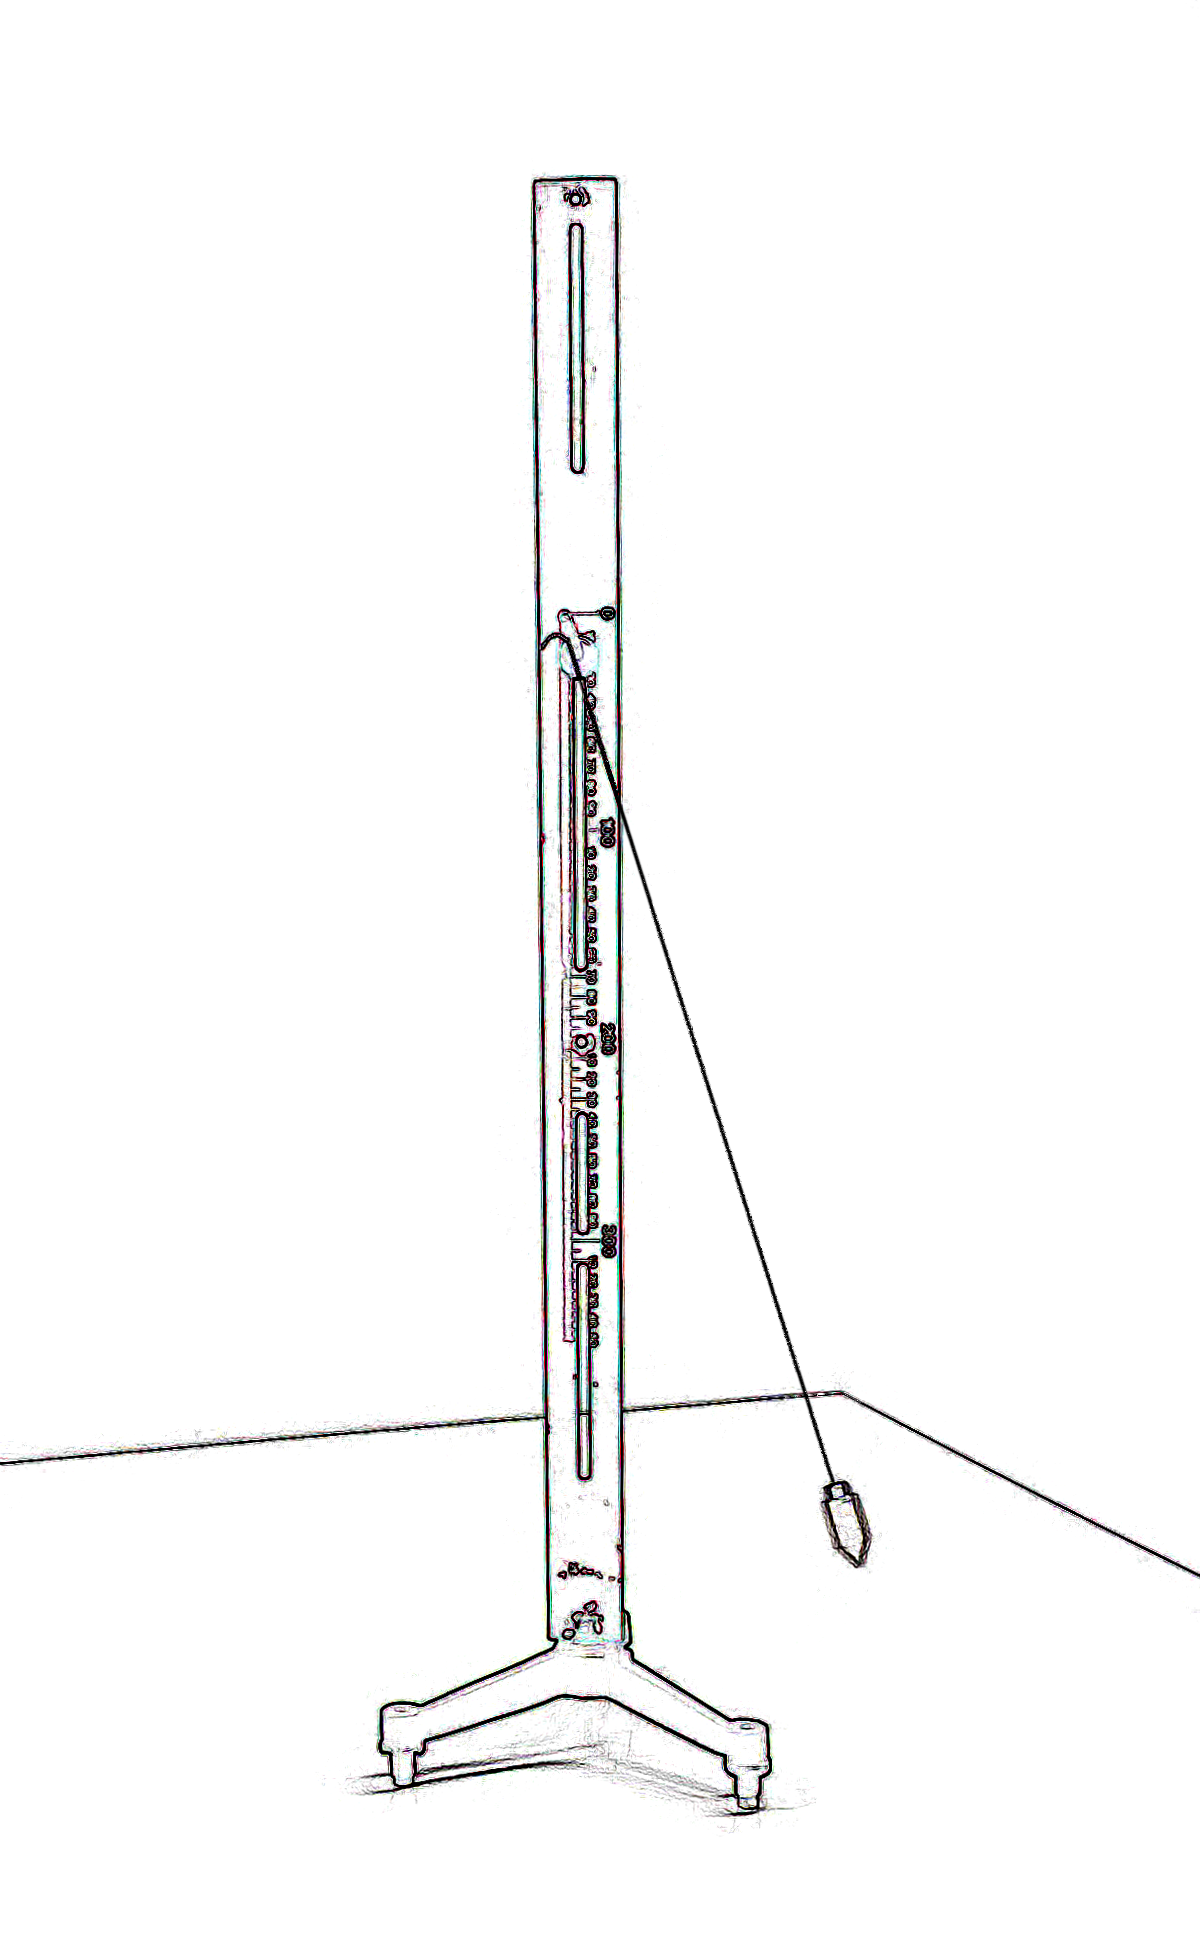
\includegraphics[width=\textwidth]{Ilustrations/Pendulo_simples.png}
	\caption{Pêndulo simples.}
\end{marginfigure}
%
onde o sinal está relacionado ao fato de que a força tem sempre direção contrária ao deslocamento. A aceleração $a$ se refere à derivada segunda da posição ao longo do arco $s$ descrito pelo objeto, portanto podemos escrever
\begin{equation}
	\frac{d^2s}{dt^2} + g\sin\theta = 0.
\end{equation}
%
\begin{marginfigure}[1cm]
\centering
\begin{tikzpicture}[>=Stealth]
	\shade[top color=white,bottom color=gray] (-1,0) rectangle +(2,0.3);
	\draw (-1,0) -- (1,0);
	\draw[dotted] (0,0) -- (0,-1.5);
	\draw (0,-3) arc[start angle = 270, end angle = 300, radius = 3] node[above, midway]{$s$} -- node[right] {$L$} (0,0);
	\draw[dotted] (canvas polar cs:radius=3cm,angle=300) arc[start angle = 300, end angle = 330, radius = 3];
	\draw (0,-0.7) arc[start angle = 270, end angle = 300, radius = 0.7] node[below = 0.05,midway] {$\theta$};
	\draw[fill] (canvas polar cs:radius=3cm,angle=300) circle[radius = 0.1] node[right=2pt] {$m$};
	\draw[->] (canvas polar cs:radius=3cm,angle=300) -- +(canvas polar cs:radius = 0.866025404 cm, angle = 120) node [midway, right]{$\vec{T}$};
	\draw[->] (canvas polar cs:radius=3cm,angle=300) -- node[left]{$\vec{P}$} +(0,-1);
	\draw[dashed,rotate=30] (canvas polar cs:radius=3cm,angle=270) ++(1,0) -- +(-2,0);
	\draw[dashed,rotate=30] (canvas polar cs:radius=3cm,angle=270) -- +(0,-1);
\end{tikzpicture}
\caption{Diagrama de corpo livre do pêndulo simples.}
\label{Fig:Pendulo}
\end{marginfigure}
%
\begin{marginfigure}[1cm]
\centering
\begin{tikzpicture}[>=Stealth,scale=1.5]
	\usetikzlibrary{calc}
	\def\centerarc[#1](#2)(#3:#4:#5)% [draw options] (center) (initial angle:final angle:radius)
	{ \draw[#1] ($(#2)+({#5*cos(#3)},{#5*sin(#3)})$) arc (#3:#4:#5); }
	\draw[fill] (0,0) circle[radius = 0.06667];
	\draw[->] (0,0) -- +(canvas polar cs:radius = 0.866025404 cm, angle = 120) node [midway, right]{$\vec{T}$};
	\draw[->] (0,0) -- node[left]{$\vec{P}$} +(0,-1);
	\draw[dashed,rotate=30] (0,0) ++(1,0) -- +(-2,0);
	\draw[dashed,rotate=30] (0,0) -- +(0,-1.2);
	\draw (0,0) +(0,-0.5) arc[start angle = 270, end angle = 300, radius = 0.5] node[below = 0.05,midway] {$\theta$};
	\draw[->,rotate=30] (0,0) -- node[above]{$P_t$} +(-0.5,0);
	\draw[dotted,rotate=30] (-0.5,-0.866025404) -- +(0,0.866025404);
	\draw[->,rotate=30] (0,0) -- node[right]{$P_r$} +(0,-0.866025404);
	\draw[dotted,rotate=30] (-0.5,-0.866025404) -- +(0.5,0);
	\centerarc[dotted](canvas polar cs:radius = 3 cm, angle = 120)(280:320:3);
\end{tikzpicture}
\caption{Decomposição da força peso em uma componente tangencial à trajetória circular e em uma componente ao longo da reta radial que liga o centro da trajetória à posição do corpo.}
\end{marginfigure}
%
Lembrando ainda que $s = L\theta$, podemos reescrever a equação acima como
\begin{equation}
	\frac{d^2\theta}{dt^2} + \frac{g}{L}\sin\theta = 0.
\end{equation}

Até este momento, a equação acima descreve o movimento de um pêndulo para qualquer valor de amplitude e, devido à função seno, não temos uma oscilação harmônica. Uma propriedade do seno, no entanto, é que para valores pequenos de $\theta$, $\sen\theta \approx \theta$. Isso pode ser visto através de uma expansão em série:
\begin{equation}
	\sen\theta = \theta -\frac{\theta^3}{3!}+\frac{\theta^5}{5!}-\frac{\theta^7}{7!}+\dots,
\end{equation}
%
onde $\theta$ é dado em radianos. Se $\theta$ é pequeno (muito menor que 1), $\theta^3$ é menor ainda, portanto os termos de ordem maior que $\theta$ são desprezíveis para pequenas oscilações. Logo
\begin{equation}
	\frac{d^2\theta}{dt^2} + \frac{g}{L}\theta = 0.
\end{equation}
%
Como a equação acima tem a mesma forma que a Equação~\ref{Eq:EquacaoDiferencialOHS}, concluímos que o movimento para o pêndulo simples também é harmônico, sendo que seu período é dado por
\begin{equation}
	T = 2\pi \sqrt{\frac{L}{g}}.
\end{equation}


%%%%%%%%%%%%%%%%%%%%%%%%%%%%%%%%%%%%%%%%%%%%%%%%%%%%%%%%%%%%%%%%%%%%%%%%%%%%%%%
\section{Experimento}
%%%%%%%%%%%%%%%%%%%%%%%%%%%%%%%%%%%%%%%%%%%%%%%%%%%%%%%%%%%%%%%%%%%%%%%%%%%%%%%

%%%%%%%%%%%%%%%%%%%%%%
\subsection{Objetivos}
%%%%%%%%%%%%%%%%%%%%%%

\begin{itemize}
	\item Verificar a relação entre o período e a massa para um sistema massa-mola.
	\item Verificar a relação entre o período e o comprimento de um pêndulo simples.
	\item Determinar a constante elástica de uma mola através do período de oscilação de um sistema massa-mola.
	\item Determinar a aceleração da gravidade através do período de oscilação de um pêndulo simples.
\end{itemize}

%%%%%%%%%%%%%%%%%%%%%%%%%%%%%%%%%%%%%%%%%%%%%%%%%%%%%%%%%%%%%%%%%%%%%%%%%%%%%%%
\section{Material Necessário}
%%%%%%%%%%%%%%%%%%%%%%%%%%%%%%%%%%%%%%%%%%%%%%%%%%%%%%%%%%%%%%%%%%%%%%%%%%%%%%%

\begin{itemize}
	\item Suporte vertical com haste horizontal;
	\item Mola;
	\item Ganchos e anilhas;
	\item Balança;
	\item Cronômetro;
	\item Fio flexível;
	\item Corpo pequeno a que se possa prender um fio;
	\item Régua milimetrada de \np[cm]{100,00}.
	\item Transferidor.
\end{itemize}

%%%%%%%%%%%%%%%%%%%%%%%%%%%%%%%%%%%%%%%%%%%%%%%%%%%%%%%%%%%%%%%%%%%%%%%%%%%%%%%
\section{Procedimento Experimental}
%%%%%%%%%%%%%%%%%%%%%%%%%%%%%%%%%%%%%%%%%%%%%%%%%%%%%%%%%%%%%%%%%%%%%%%%%%%%%%%

%%%%%%%%%%%%%%%%%%%%%%%%%%%%%%%
\subsection{Sistema massa-mola}
%%%%%%%%%%%%%%%%%%%%%%%%%%%%%%%

\begin{enumerate}
\item Prenda uma extremidade da mola à haste horizontal do suporte e a disponha verticalmente.
\item Afira a massa de um gancho com uma anilha, anotando o valor na Tabela~\ref{Tab:DadosMassaMola}. Prenda-os à extremidade inferior da mola.
\item Desloque o gancho e a anilha alguns centímetros para baixo e solte. Deixe o sistema completar 10 oscilações, cronometrando o tempo necessário para efetuá-las. Cuidado para não exceder a amplitude máxima para a compressão da mola. Utilize como erro para o cronômetro\footnote{Em um cronômetro manual, o erro é dominado pelo tempo de reação do operador. Por isso, o valor típico do desvio padrão de uma medida efetuada com um cronômetro deste tipo não coincide com o valor da menor divisão da escala --~se o equipamento for não-analógico~--, ou com a metade dela --~se o equipamento for analógico~--.} o valor de \np[s]{0,2}.
\item Anote os resultados para o tempo necessário para completar as 10 oscilações na Tabela~\ref{Tab:DadosMassaMola}. Utilize unidades do SI.
\item Adicione anilhas ao gancho, uma a uma, e repita o processo acima para cada adição. Anote os valores de massa do gancho com as anilhas e o tempo correspondente de oscilação. Adicione tantas anilhas quanto possível, tomando o cuidado de não danificar a mola.
\end{enumerate}

%%%%%%%%%%%%%%%%%%%%%%%%%%%%
\subsection{Pêndulo simples}
%%%%%%%%%%%%%%%%%%%%%%%%%%%%

\begin{enumerate}
	\item Prenda o corpo pequeno à extremidade de um fio flexível.
	\item Prenda prenda a outra extremidade do fio à haste horizontal do suporte, de forma que a distância entre a haste de sustentação e o centro de massa do corpo seja de aproximadamente \np[cm]{100,00}. Solte o corpo de forma que o fio fique esticado e o corpo se mantenha parado, sustentado pelo fio.
	\item Desloque o corpo lateralmente, de forma que o ângulo entre o fio e a vertical não exceda \np[\tcdegree]{10,0}. Deixe o corpo completar 10 oscilações, cronometrando o tempo necessário. Anote o valor do comprimento do fio e do tempo para as 10 oscilações na Tabela~\ref{Tab:DadosPendulo}. Utilize unidades do SI.
	\item Diminua o tamanho do fio em \np[cm]{5,00} e calcule o novo tempo necessário para completar as 10 oscilações, anotando as informações na Tabela~\ref{Tab:DadosPendulo}.
	\item Repita o processo acima até um comprimento mínimo de \np[cm]{45,00}.
\end{enumerate}


%%%%%%%%%%%%%%%%%%%%%%%%%%%%%%%%%%%%%%%%%%%%%%%%%%%%%%%%%%%%%%%%%%%%%%%%%%%%%%%
%%%%%%%%%%%%%%%%%%%%%%%%%%%%%%%%%%%%%%%%%%%%%%%%%%%%%%%%%%%%%%%%%%%%%%%%%%%%%%%
%%%%%%%%%%%%%%%%%%%%%%%%%%%%%%%%%%%%%%%%%%%%%%%%%%%%%%%%%%%%%%%%%%%%%%%%%%%%%%%
%%%%%%%%%%%%%%%%%%%%%%%%%%%%%%%%%%%%%%%%%%%%%%%%%%%%%%%%%%%%%%%%%%%%%%%%%%%%%%%
\cleardoublepage

\noindent{}{\huge\textit{Oscilações}}

\vspace{15mm}

\begin{fullwidth}
\noindent{}\makebox[0.6\linewidth]{Turma:\enspace\hrulefill}\makebox[0.4\textwidth]{  Data:\enspace\hrulefill}
\vspace{5mm}

\noindent{}\makebox[0.6\linewidth]{Aluno(a):\enspace\hrulefill}\makebox[0.4\textwidth]{  Matrícula:\enspace\hrulefill}

\noindent{}\makebox[0.6\linewidth]{Aluno(a):\enspace\hrulefill}\makebox[0.4\textwidth]{  Matrícula:\enspace\hrulefill}

\noindent{}\makebox[0.6\linewidth]{Aluno(a):\enspace\hrulefill}\makebox[0.4\textwidth]{  Matrícula:\enspace\hrulefill}

\noindent{}\makebox[0.6\linewidth]{Aluno(a):\enspace\hrulefill}\makebox[0.4\textwidth]{  Matrícula:\enspace\hrulefill}

\noindent{}\makebox[0.6\linewidth]{Aluno(a):\enspace\hrulefill}\makebox[0.4\textwidth]{  Matrícula:\enspace\hrulefill}
\end{fullwidth}

\vspace{5mm}

%%%%%%%%%%%%%%%%%%%%%%%%%%%%%%%%%%%%%%%%%%%%%%%%%%%%%%%%%%%%%%%%%%%%%%%%%%%%%%%
\section{Questionário}
%%%%%%%%%%%%%%%%%%%%%%%%%%%%%%%%%%%%%%%%%%%%%%%%%%%%%%%%%%%%%%%%%%%%%%%%%%%%%%%

\begin{question}[type={exam}]{1}
Apresente os resultados de maneira clara e organizada. Mostre os cálculos requisitados de maneira clara e sucinta, evidenciando o raciocínio desenvolvido.
\end{question}

\begin{question}[type={exam}]{0.75}
Liste os equipamentos utilizados descrevendo o tipo do equipamento, sua resolução, e qual é o seu erro de escala.
\end{question}

\begin{question}[type={exam}]{0.75}
Preencha as tabelas com o número adequado de algarismos significativos, unidades, e erros de escala apropriados. 
\end{question}

\begin{question}[type={exam}]{1.5}
Elabore um gráfico de $T^2 \times m$ para os dados da Tabela~\ref{Tab:DadosMassaMola}. Calcule a reta que melhor representa os dados experimentais utilizando o método dos mínimos quadrados. Mostre a relação entre o coeficiente angular $B$ e a constante da mola $k$, e calcule o valor desta última. \emph{Utilize as unidades do SI para efetuar a regressão linear para obter resultados de mais fácil interpretação.}
\end{question}
 
\begin{question}[type={exam}]{1.5}
Elabore um gráfico de $T^2 \times L$ para os dados da Tabela~\ref{Tab:DadosPendulo}. Calcule a reta que melhor representa os dados experimentais utilizando o método dos mínimos quadrados. Mostre a relação entre o coeficiente angular $B$ e a aceleração da gravidade $g$, e calcule o valor desta última. \emph{Utilize as unidades do SI para efetuar a regressão linear para obter resultados de mais fácil interpretação.}
\end{question}

\begin{question}[type={exam}]{1.5}
Calcule o erro associado ao coeficiente angular para a regressão linear dos dados de $T^2 \times m$. Com esse valor e o do próprio coeficiente, calcule o erro associado à constante da mola $k$.
\end{question}

\begin{question}[type={exam}]{1.5}
Calcule o erro associado ao coeficiente angular para a regressão linear dos dados de $T^2 \times L$. Com esse valor e o do próprio coeficiente, calcule o erro associado à constante da mola $g$.
\end{question}

\begin{question}[type={exam}]{1.5}
Através dos resultados obtidos nas questões anteriores, discuta quais objetivos foram atingidos com sucesso, justificando suas conclusões. Se algum objetivo não foi atingido, discuta quais são os possíveis motivos do fracasso e que providências podem ser tomadas para que eles sejam alcançados.
\end{question}

%%%%%%%%%%%%%%%%%%%%%%%%%%%%%%%%%%%%%%%%%%%%%%%%%%%%%%%%%%%%%%%%%%%%%%%%%%%%%%%
\section{Tabelas}
%%%%%%%%%%%%%%%%%%%%%%%%%%%%%%%%%%%%%%%%%%%%%%%%%%%%%%%%%%%%%%%%%%%%%%%%%%%%%%%
\begin{table*}[!htb]
\caption{Dados para a oscilação de um sistema massa-mola e de um pêndulo simples.}
\label{Tab:DadosMassaMola}
	\begin{center}
		\begin{tabular}{p{25mm}p{25mm}p{25mm}p{25mm}}
		\toprule
		$m$ & $T_{10}$ & $T$ & $T^2$ \\
		\midrule
		\cellcolor[gray]{0.89} & \cellcolor[gray]{0.92} & \cellcolor[gray]{0.89} & \cellcolor[gray]{0.92} \\
		\cellcolor[gray]{0.95} & \cellcolor[gray]{0.97} & \cellcolor[gray]{0.95} & \cellcolor[gray]{0.97} \\
		\cellcolor[gray]{0.89} & \cellcolor[gray]{0.92} & \cellcolor[gray]{0.89} & \cellcolor[gray]{0.92} \\
		\cellcolor[gray]{0.95} & \cellcolor[gray]{0.97} & \cellcolor[gray]{0.95} & \cellcolor[gray]{0.97} \\
		\cellcolor[gray]{0.89} & \cellcolor[gray]{0.92} & \cellcolor[gray]{0.89} & \cellcolor[gray]{0.92} \\
		\cellcolor[gray]{0.95} & \cellcolor[gray]{0.97} & \cellcolor[gray]{0.95} & \cellcolor[gray]{0.97} \\
		\bottomrule
		\end{tabular}
	\end{center}
\end{table*}
%
%
\begin{table*}[!htb]
	\caption{Dados para a oscilação de um pêndulo.}
	\label{Tab:DadosPendulo}
	\begin{center}
		\begin{tabular}{p{25mm}p{25mm}p{25mm}p{25mm}}
		\toprule
		  $L$ & $T_{10}$ & $T$ & $T^2$\\
		\midrule
		\cellcolor[gray]{0.89} & \cellcolor[gray]{0.92} & \cellcolor[gray]{0.89} & \cellcolor[gray]{0.92} \\
		\cellcolor[gray]{0.95} & \cellcolor[gray]{0.97} & \cellcolor[gray]{0.95} & \cellcolor[gray]{0.97} \\
		\cellcolor[gray]{0.89} & \cellcolor[gray]{0.92} & \cellcolor[gray]{0.89} & \cellcolor[gray]{0.92} \\
		\cellcolor[gray]{0.95} & \cellcolor[gray]{0.97} & \cellcolor[gray]{0.95} & \cellcolor[gray]{0.97} \\
		\cellcolor[gray]{0.89} & \cellcolor[gray]{0.92} & \cellcolor[gray]{0.89} & \cellcolor[gray]{0.92} \\
		\cellcolor[gray]{0.95} & \cellcolor[gray]{0.97} & \cellcolor[gray]{0.95} & \cellcolor[gray]{0.97} \\
		\cellcolor[gray]{0.89} & \cellcolor[gray]{0.92} & \cellcolor[gray]{0.89} & \cellcolor[gray]{0.92} \\
		\cellcolor[gray]{0.95} & \cellcolor[gray]{0.97} & \cellcolor[gray]{0.95} & \cellcolor[gray]{0.97} \\
		\cellcolor[gray]{0.89} & \cellcolor[gray]{0.92} & \cellcolor[gray]{0.89} & \cellcolor[gray]{0.92} \\
		\cellcolor[gray]{0.95} & \cellcolor[gray]{0.97} & \cellcolor[gray]{0.95} & \cellcolor[gray]{0.97} \\
		\cellcolor[gray]{0.89} & \cellcolor[gray]{0.92} & \cellcolor[gray]{0.89} & \cellcolor[gray]{0.92} \\
		\cellcolor[gray]{0.95} & \cellcolor[gray]{0.97} & \cellcolor[gray]{0.95} & \cellcolor[gray]{0.97} \\
		\bottomrule
		\end{tabular}
	\end{center}
\end{table*}

%%%%%%%%%%%%%%%%%%%%%%%%%%%%%%%%%%%%%%%%%%%%%%%%%%%%%%%%%%%%%%%%%%%%%%%%%%%%%%%%
\chapter{Pêndulo Físico} % Sem "Experiência 01" ou qualquer outro número
\label{Chap:PenduloFisico} % para poder trocar a ordem com facilidade
%%%%%%%%%%%%%%%%%%%%%%%%%%%%%%%%%%%%%%%%%%%%%%%%%%%%%%%%%%%%%%%%%%%%%%%%%%%%%%%

\begin{fullwidth}\it
	Que experimento faremos?
	Qual é o objetivo?
	O que veremos/revisaremos? (teoria física)
	Quais conceitos/técnicas de análise de dados utilizaremos?
\end{fullwidth}

%%%%%%%%%%%%%%%%%%%%%%%%%%%%%%%%%%%%%%%%%%%%%%%%%%%%%%%%%%%%%%%%%%%%%%%%%%%%%%%
\section{Física do experimento}
%%%%%%%%%%%%%%%%%%%%%%%%%%%%%%%%%%%%%%%%%%%%%%%%%%%%%%%%%%%%%%%%%%%%%%%%%%%%%%%

%%%%%%%%%%%%%%%%%%%%%%%%%%%%%%%%%%%%%%%%%%%%%
%\subsection{Se necessário, usar subsections}
%%%%%%%%%%%%%%%%%%%%%%%%%%%%%%%%%%%%%%%%%%%%%

%%%%%%%%%%%%%%%%%%%%%%%%%%%%%%%%%%%%%%%%%%%%%%%%%%%%%%%%%%%%%%%%%%%%%%%%%%%%%%%
\section{Experimento}
%%%%%%%%%%%%%%%%%%%%%%%%%%%%%%%%%%%%%%%%%%%%%%%%%%%%%%%%%%%%%%%%%%%%%%%%%%%%%%%

%%%%%%%%%%%%%%%%%%%%%%
\subsection{Objetivos}
%%%%%%%%%%%%%%%%%%%%%%

\begin{itemize}
	\item Resultados concretos que devemos conseguir;
	\item Observar a relação de tal coisa com outra coisa;
	\item Calcular a constante $x$.
\end{itemize}

%%%%%%%%%%%%%%%%%%%%%%%%%%%%%%%%%%%%%%%%%%%%%%%%%%%%%%%%%%%%%%%%%%%%%%%%%%%%%%%
\section{Material Necessário}
%%%%%%%%%%%%%%%%%%%%%%%%%%%%%%%%%%%%%%%%%%%%%%%%%%%%%%%%%%%%%%%%%%%%%%%%%%%%%%%

\begin{itemize}
	\item Item 1;
	\item Item 2.
\end{itemize}

%%%%%%%%%%%%%%%%%%%%%%%%%%%%%%%%%%%%%%%%%%%%%%%%%%%%%%%%%%%%%%%%%%%%%%%%%%%%%%%
\section{Procedimento Experimental}
%%%%%%%%%%%%%%%%%%%%%%%%%%%%%%%%%%%%%%%%%%%%%%%%%%%%%%%%%%%%%%%%%%%%%%%%%%%%%%%

%%%%%%%%%%%%%%%%%%%%%
%\subsection{Parte A} % Se necessário
%%%%%%%%%%%%%%%%%%%%%
\begin{enumerate}
	\item Passo 1;
	\item Passo 2;
	\item Passo 3.
\end{enumerate}

%%%%%%%%%%%%%%%%%%%%%%%%%%%%%%%%%%%%%%%%%%%%%%%%%%%%%%%%%%%%%%%%%%%%%%%%%%%%%%%
%%%%%%%%%%%%%%%%%%%%%%%%%%%%%%%%%%%%%%%%%%%%%%%%%%%%%%%%%%%%%%%%%%%%%%%%%%%%%%%
%%%%%%%%%%%%%%%%%%%%%%%%%%%%%%%%%%%%%%%%%%%%%%%%%%%%%%%%%%%%%%%%%%%%%%%%%%%%%%%
%%%%%%%%%%%%%%%%%%%%%%%%%%%%%%%%%%%%%%%%%%%%%%%%%%%%%%%%%%%%%%%%%%%%%%%%%%%%%%%
\cleardoublepage

\noindent{}{\huge\textit{Pêndulo Físico}}

\vspace{15mm}

\begin{fullwidth}
\noindent{}\makebox[0.6\linewidth]{Turma:\enspace\hrulefill}\makebox[0.4\textwidth]{  Data:\enspace\hrulefill}
\vspace{5mm}

\noindent{}\makebox[0.6\linewidth]{Aluno(a):\enspace\hrulefill}\makebox[0.4\textwidth]{  Matrícula:\enspace\hrulefill}

\noindent{}\makebox[0.6\linewidth]{Aluno(a):\enspace\hrulefill}\makebox[0.4\textwidth]{  Matrícula:\enspace\hrulefill}

\noindent{}\makebox[0.6\linewidth]{Aluno(a):\enspace\hrulefill}\makebox[0.4\textwidth]{  Matrícula:\enspace\hrulefill}

\noindent{}\makebox[0.6\linewidth]{Aluno(a):\enspace\hrulefill}\makebox[0.4\textwidth]{  Matrícula:\enspace\hrulefill}

\noindent{}\makebox[0.6\linewidth]{Aluno(a):\enspace\hrulefill}\makebox[0.4\textwidth]{  Matrícula:\enspace\hrulefill}
\end{fullwidth}

\vspace{5mm}

%%%%%%%%%%%%%%%%%%%%%%%%%%%%%%%%%%%%%%%%%%%%%%%%%%%%%%%%%%%%%%%%%%%%%%%%%%%%%%%
\section{Questionário}
%%%%%%%%%%%%%%%%%%%%%%%%%%%%%%%%%%%%%%%%%%%%%%%%%%%%%%%%%%%%%%%%%%%%%%%%%%%%%%%
\emph{Nas questões seguintes, apresente os cálculos requisitados de maneira clara e sucinta, para que o professor possa acompanhar o raciocínio desenvolvido.}
\vspace{5mm}

\begin{question}[type={exam}]{2}
Lorem ipsum dolor sit amet, consectetuer adi-
piscing elit. Ut purus elit, vestibulum ut, placerat ac, adipiscing vitae,
felis. Curabitur dictum gravida mauris. Nam arcu libero, nonummy
eget, consectetuer id, vulputate a, magna. Donec vehicula augue
eu neque. Pellentesque habitant morbi tristique senectus et netus
et malesuada fames ac turpis egestas. Mauris ut leo. Cras viverra
metus rhoncus sem. Nulla et lectus vestibulum urna fringilla ultrices.
\end{question}

\begin{question}[type={exam}]{2}
Lorem ipsum dolor sit amet, consectetuer adi-
piscing elit. Ut purus elit, vestibulum ut, placerat ac, adipiscing vitae,
felis. Curabitur dictum gravida mauris. Nam arcu libero, nonummy
eget, consectetuer id, vulputate a, magna. Donec vehicula augue
eu neque. Pellentesque habitant morbi tristique senectus et netus
et malesuada fames ac turpis egestas. Mauris ut leo. Cras viverra
metus rhoncus sem. Nulla et lectus vestibulum urna fringilla ultrices.
\end{question}

\begin{question}[type={exam}]{2}
Lorem ipsum dolor sit amet, consectetuer adi-
piscing elit. Ut purus elit, vestibulum ut, placerat ac, adipiscing vitae,
felis. Curabitur dictum gravida mauris. Nam arcu libero, nonummy
eget, consectetuer id, vulputate a, magna. Donec vehicula augue
eu neque. Pellentesque habitant morbi tristique senectus et netus
et malesuada fames ac turpis egestas. Mauris ut leo. Cras viverra
metus rhoncus sem. Nulla et lectus vestibulum urna fringilla ultrices.
\end{question}

\begin{question}[type={exam}]{2}
Lorem ipsum dolor sit amet, consectetuer adi-
piscing elit. Ut purus elit, vestibulum ut, placerat ac, adipiscing vitae,
felis. Curabitur dictum gravida mauris. Nam arcu libero, nonummy
eget, consectetuer id, vulputate a, magna. Donec vehicula augue
eu neque. Pellentesque habitant morbi tristique senectus et netus
et malesuada fames ac turpis egestas. Mauris ut leo. Cras viverra
metus rhoncus sem. Nulla et lectus vestibulum urna fringilla ultrices.
\end{question}

\begin{question}[type={exam}]{2}
Lorem ipsum dolor sit amet, consectetuer adi-
piscing elit. Ut purus elit, vestibulum ut, placerat ac, adipiscing vitae,
felis. Curabitur dictum gravida mauris. Nam arcu libero, nonummy
eget, consectetuer id, vulputate a, magna. Donec vehicula augue
eu neque. Pellentesque habitant morbi tristique senectus et netus
et malesuada fames ac turpis egestas. Mauris ut leo. Cras viverra
metus rhoncus sem. Nulla et lectus vestibulum urna fringilla ultrices.
\end{question}
\vfill
%%%%%%%%%%%%%%%%%%%%%%%%%%%%%%%%%%%%%%%%%%%%%%%%%%%%%%%%%%%%%%%%%%%%%%%%%%%%%%%
\pagebreak
\section{Tabelas}
%%%%%%%%%%%%%%%%%%%%%%%%%%%%%%%%%%%%%%%%%%%%%%%%%%%%%%%%%%%%%%%%%%%%%%%%%%%%%%%


%%%%%%%%%%%%%%%%%%%%%%%%%%%%%%%%%%%%%%%%%%%%%%%%%%%%%%%%%%%%%%%%%%%%%%%%%%%%%%%
\chapter{Ondas estacionárias}
\label{Chap:ExpOndasEstacionarias}
%%%%%%%%%%%%%%%%%%%%%%%%%%%%%%%%%%%%%%%%%%%%%%%%%%%%%%%%%%%%%%%%%%%%%%%%%%%%%%%

\begin{fullwidth}\it
Submeteremos um fio a uma tensão e a uma vibração, com a consequente formação de ondas estacionárias. O objetivo desse experimento é verificarmos experimentalmente as propriedades de tais ondas e as relações com os diversos parâmetros do sistema. Utilizaremos os seguintes conceitos/técnicas de análise de dados: medidas, algarismos significativos, gráficos, software para elaboração de gráficos, erros de escala e propagados, equação geral para o erro propagado, regressão linear, linearização, e erros dos coeficientes $A$ e $B$.
\end{fullwidth}

%%%%%%%%%%%%%%%%%%%%%%%%%%%%%%%%%%%%%%%%%%%%%%%%%%%%%%%%%%%%%%%%%%%%%%%%%%%%%%%
\section{Ondas transversais}
%%%%%%%%%%%%%%%%%%%%%%%%%%%%%%%%%%%%%%%%%%%%%%%%%%%%%%%%%%%%%%%%%%%%%%%%%%%%%%%

\begin{marginfigure}[5cm]
\centering
\begin{tikzpicture}[>=Stealth,domain=0:3.1415,samples=50]
	\draw[->] (-0.5,0) -- (4,0) node[below]{$x$};
	\draw[<-] (0,1.5) node[left]{$y$} -- (0,-1.5);
	\draw[color = black,smooth] plot (\x,{sin(2 * \x r)});
	
	\draw[dotted] (3.1415,-1.2) -- (3.1415,0);
	\draw[<->] (0,-1.2) -- node[below]{$\lambda$} (3.1415,-1.2);
	\draw[<->] (0.7854,0) -- node[right]{$A$} (0.7854,1);
\end{tikzpicture}
\caption{Parâmetros espaciais de uma onda transversal.}
\label{Fig:OndaCongelada}
\end{marginfigure}

\begin{marginfigure}
\centering
\begin{tikzpicture}[>=Stealth,domain=0:3.1415,samples=50]
	\draw[->] (-0.5,0) -- (4,0) node[below]{$t$};
	\draw[<-] (0,1.5) node[left]{$y$} -- (0,-1.5);
	\draw[color = black,smooth] plot (\x,{sin(2 * \x r)});
	
	\draw[dotted] (3.1415,-1.2) -- (3.1415,0);
	\draw[<->] (0,-1.2) -- node[below]{$T$} (3.1415,-1.2);
	\draw[<->] (0.7854,0) -- node[right]{$A$} (0.7854,1);
\end{tikzpicture}
\caption{Parâmetros temporais de uma onda transversal.}
\label{Fig:OscilacaoPontoOnda}
\end{marginfigure}

Uma onda mecânica é uma perturbação periódica que se propaga em um meio. No caso de uma onda transversal, tal perturbação é um deslocamento lateral, perpendicular à direção de propagação da onda. Esse tipo de onda pode ser descrita como uma função $y(x,t)$, onde $y$ representa o valor da perturbação na posição $x$ e tempo $t$. A forma mais simples para essa função é
\begin{equation}\label{Eq:OndaUnidimensional}
	y(x,t) = A \sen(kx - \omega t),
\end{equation}
%
onde $A$ é a amplitude da onda ---~isto é, o valor máximo atingido pela variável $y$~--- e os parâmetros $k$ e $\omega$ são denominados como \emph{número de onda} e \emph{frequência angular}, respectivamente.

Tal expressão pode ser entendida de maneira simples se considerarmos dois casos especiais: $x = 0$ para qualquer $t$ e $t = 0$ para qualquer $x$. Isso resulta nas expressões
\begin{equation}
	y(t) = A \sen (\omega t),
\end{equation}
%
e
\begin{equation}
	y(x) = A \sen(kx).
\end{equation}
%
O primeiro caso representa simplesmente a oscilação de um ponto do meio no qual a onde se propaga (especificamente, nesse caso, aquele localizado na origem do eixo $x$). No segundo caso, temos uma análise de toda a onda em um dado instante de tempo, como se a fotografássemos (veja a Figura~\ref{Fig:OndaCongelada}).

%%%%%%%%%%%%%%%%%%%%%%%%%%%%%%%%%%%%%%%%%%%%%%%%%%%%%%%%%%%%%
\paragraph{Interpretação da frequência angular para uma onda}
%%%%%%%%%%%%%%%%%%%%%%%%%%%%%%%%%%%%%%%%%%%%%%%%%%%%%%%%%%%%%

Sabemos que o a função $\sen \theta$ se repete a partir de $\theta = 2\pi$, o que se reflete em uma repetição do movimento oscilatório. Consequentemente, temos que ao final de uma oscilação
\begin{equation}
	\omega T = 2 \pi,
\end{equation}
%
onde usamos $t = T$ ---~isto é, a variável $t$ assume o valor do período $T$ da oscilação (o tempo que o movimento oscilatório demora para completar um ciclo)~---. Logo
\begin{equation}
	\omega = \frac{2 \pi}{T}.
\end{equation}
%
Para determinarmos o número de oscilações por unidade de tempo ---~a frequência da oscilação~---, basta dividirmos uma unidade de tempo pela duração de uma oscilação, ou seja,
\begin{equation}
	f = \frac{1}{T},
\end{equation}
%
o que nos permite escrever
\begin{equation}
	\omega = 2 \pi f.
\end{equation}

%%%%%%%%%%%%%%%%%%%%%%%%%%%%%%%%%%%%%%%%%%%
\paragraph{Interpretação do número de onda}
%%%%%%%%%%%%%%%%%%%%%%%%%%%%%%%%%%%%%%%%%%%

Se nos deslocamos na direção do eixo $x$, observamos uma variação da posição $y$, sendo que após percorrermos uma distância $\lambda$ ---~denominada \emph{comprimento de onda}~--- o movimento se repete. Novamente, como a função $\sen\theta$ se repete após $\theta = 2\pi$, temos que para a posição $x = \lambda$
\begin{equation}
	k \lambda = 2\pi,
\end{equation}
%
ou
\begin{equation}
	k = \frac{2\pi}{\lambda}.
\end{equation}

%%%%%%%%%%%%%%%%%%%%%%%%%%%%%%%%%%%%%%%%%%%%%%%%
\paragraph{Velocidade de propagação de uma onda}
%%%%%%%%%%%%%%%%%%%%%%%%%%%%%%%%%%%%%%%%%%%%%%%%

Podemos calcular a velocidade de propagação da onda simplesmente verificando que uma crista qualquer (o ponto em que $y$ atinge o valor máximo) se desloca uma distância $\lambda$ a cada oscilação. Logo
\begin{equation}\label{Eq:RelVelFreqAngNumOnda}
	v = \frac{\lambda}{T} = \lambda f = \frac{\omega}{k}.
\end{equation}
%
A velocidade de propagação de uma onda é uma constante que depende de características do meio no qual ela se propaga. Em uma onda transversal em uma corda, por exemplo, ela é dada por
\begin{equation}\label{Eq:VelocidadeOndaEmUmaCorda}
    v = \sqrt{\frac{T}{\mu}},
\end{equation}
%
onde $T$ representa a tensão a qual a corda está submetida, e $\mu$ representa a densidade linear de massa da corda. Portanto, os valores da frequência angular $\omega$ e do número de onda $k$ não são independentes, pois estão ligados através da velocidade.

%%%%%%%%%%%%%%%%%%%%%%%%%%%%%%%%%%%%%%%%%%%%%
\paragraph{Sentido de propagação de uma onda}
%%%%%%%%%%%%%%%%%%%%%%%%%%%%%%%%%%%%%%%%%%%%%

O sentido de propagação da onda está ligado ao sinal do termo $\omega t$ na Equação~\eqref{Eq:OndaUnidimensional}. Podemos entender tal relação se consideramos um sistema de referência ortogonal $xy$ e uma onda que se propaga no sentido positivo do eixo $x$, como mostrado na Figura~\ref{Fig:SinalPropOndaSentidoPositivo}. No referencial $xy$, a onda é descrita através de uma função $y(x,t)$ e se propaga com velocidade $v$.

\begin{marginfigure}
\centering
\begin{tikzpicture}[>=Stealth]

    \draw[densely dotted, ->] (-0.5,0) -- (3.5,0) node[below left]{$x$};
    \draw[densely dotted, ->] (0,-1.5) -- (0,1.5) node[below left]{$y$};
    
	\draw[smooth, domain=-0.5:3.2,samples=50] plot (\x,{sin(2 * \x r)});
    
    \draw [->] (1.25,0) -- (2.75,0) node[above left]{$x'$};
    \draw [->] (1.25,0) -- (1.25,1.25) node[left]{$y'$};

    \draw [dotted] (1.25,0) -- (1.25, -0.5);    
    \draw [|<->|] (0, -0.5) -- node[below]{$v\cdot t$} (1.25, -0.5);
    
    \draw[->] (1.25, 1) -- (2,1) node[above]{$\vec{v}$};

\end{tikzpicture}
\caption{Para uma onda que se propagan no sentido positivo de $x$, a relação entre as coordenadas $x$ e $x'$ é $x' = x - vt$.\label{Fig:SinalPropOndaSentidoPositivo}}
\end{marginfigure}

Em um segundo referencial ortogonal, denotado $x'y'$, que se move na direção e sentido do eixo $x$, com velocidade $v$ em relação ao primeiro sistema de referência, temos que a velocidade da onda é nula. A função $y'$ que descreve a onda deve então depender somente da posição $x'$ nesse referencial, ou seja, temos somente $y'(x')$. Podemos assumir que no referencial $x'y'$ a expressão para a onda é dada por
\begin{equation}
    y'(x') = A\sen(kx').
\end{equation}
%
A relação entre $x'$ e $x$ é dada por
\begin{equation}
    x' = x - vt,
\end{equation}
%
portanto, podemos escrever $y'(x,t)$ como
\begin{align}
    y'(x,t) &= A\sen(k[x - vt]) \\
    &= A\sen(kx - kvt).
\end{align}    

Considerando que a origem dos eixos $y$ e $y'$ coincide, podemos escrever $y'(x,t) = y(x,t)$, o que nos permite escrever
\begin{equation}
    y(x,t) = A\sen(kx - \omega t), \mathnote{Onda transversal que se propaga no sentido positivo}
\end{equation}
%
onde utilizamos a Equação~\ref{Eq:RelVelFreqAngNumOnda} para eliminar a velocidade. Note, portanto, que no caso em que a onda se desloca no sentido \emph{positivo}, o sinal deve ser \emph{negativo}.

\begin{marginfigure}[3cm]
\centering
\begin{tikzpicture}[>=Stealth]

    \draw[densely dotted, ->] (-0.5,0) -- (3.5,0) node[below left]{$x$};
    \draw[densely dotted, ->] (2.5,-1.5) -- (2.5,1.5) node[below left]{$y$};
    
	\draw[smooth, domain=-0.5:3.2,samples=50] plot (\x,{sin(2 * \x r)});
    
    \draw [->] (0.4,0) -- (1.5,0) node[below left]{$x'$};
    \draw [->] (0.4,0) -- (0.4,1.25) node[left]{$y'$};

    \draw [dotted] (0.4,0) -- (0.4, -0.5);    
    \draw [|<->|] (0.4, -0.5) -- node[below]{$v\cdot t$} (2.5, -0.5);
    
    \draw[->] (0.4, 1) -- (-0.1,1) node[below]{$\vec{v}$};

\end{tikzpicture}
\caption{No caso de uma onda que se propagan no sentido negativo de $x$, a relação entre as coordenadas $x$ e $x'$ é $x' = x + vt$.\label{Fig:SinalPropOndaSentidoNegativo}.}
\end{marginfigure}

Caso a onda se desloque no sentido negativo do eixo $x$, novamente com um sistema de referência ortogonal $x'y'$ que se move na mesma direção e sentido para a qual a onda se propaga ---~como mostrado na Figura~\ref{Fig:SinalPropOndaSentidoNegativo}~---, temos como única diferença o fato de que a relação entre $x'$ e $x$ é dada por
\begin{equation}
    x' = x + vt,
\end{equation}
%
de onde obtemos
\begin{equation}
    y(x,t) = A\sen(kx + \omega t). \mathnote{Onda transversal que se propaga no sentido negativo}
\end{equation}
%
Portanto, se a onda se desloca no sentido \emph{negativo} do eixo $x$, temos um sinal \emph{positivo}.

\begin{marginfigure}[2cm]
\centering
\begin{tikzpicture}[>=Stealth]

    \draw[->] (0,0) -- (4,0) node[below left]{$x$};
    \draw[->] (0,-1.5) -- (0,1.5) node[below left]{$y$};
    
    \draw (1.4,0) -- +(0,1);
    \draw (0.8,0.6754) -- +(1,0);
	\draw[smooth, domain=0:3.1415,samples=50] plot (\x,{sin(2 * \x r)});
    \draw[fill] (1.4,0.335) circle (1pt);
    \draw[fill = white, draw = black] (1.2,0.6754) circle (1pt);
    
	\draw[smooth, dotted, domain=0:3.1415,samples=50] plot (\x,{sin(2 * (\x - 0.2) r)});
	
	\draw[fill = white, draw = black] (1.4,0.6754) circle (1pt);
     	
\end{tikzpicture}
\caption{Ao aumentarmos o valor de $t$, temos uma diminuição do valor do argumento da função seno. Poderíamos ter uma diminuição equivalente reduzindo o valor de $x$, o que equivale a alterar a posição do ponto preenchido para o ponto vazado. Tal alteração equivale, por sua vez, a deslocar todo o gráfico para a direita.}
\end{marginfigure}

Uma maneira alternativa de compreender a relação entre o sinal e o sentido de propagação é a de que se tomarmos um valor de $x$ qualquer com um valor de $\sen(kx-\omega t)$ correspondente, quando $t$ aumenta, o valor do argumento ---~isto é, $kx -\omega t$~--- diminui. Equivalentemente, poderíamos simplesmente diminuir o argumento escolhendo um valor de $x$ menor, ou seja, escolheríamos um ponto à esquerda. O efeito de aumentar o $t$ é então o de tomar o ``gráfico'' do $\sen(kx)$ e deslocá-lo para a direita, o que implica em uma propagação da onda para a direita. Logo, para uma onda que se propaga no sentido positivo
\begin{equation}
    y(x,t) = A\sen(kx -\omega t).
\end{equation}

\begin{figure*}[t]
\centering
\forceversofloat

\tikzfading[name=fade right, left color=transparent!100, right color=transparent!0]

\begin{tikzpicture}[>=Stealth,domain=0:13,samples=250]

	\draw[color = gray!05,smooth,thick] plot (\x,{1.7 * sin(\x r)});
	\draw[color = gray!10,smooth,thick] plot (\x,{1.7 * sin((\x - 0.1) r)});
	\draw[color = gray!20,smooth,thick] plot (\x,{1.7 * sin((\x - 0.2) r)});
	\draw[color = gray!40,smooth,thick] plot (\x,{1.7 * sin((\x - 0.3) r)});
	\draw[color = gray!60,smooth,thick] plot (\x,{1.7 * sin((\x - 0.4) r)});
	\draw[color = gray!80,smooth,thick] plot (\x,{1.7 * sin((\x - 0.5) r)});
	\draw[color = gray,smooth,thick] plot (\x,{1.7 * sin((\x - 0.6) r)});		
	\draw[color = black,smooth,thick] plot (\x,{1.7 * sin((\x - 0.7) r)});
	
	\fill [white,path fading=fade right] (12,-2) rectangle (13.01,2);
	
	\draw[<-] (0,2) node[left]{$y$} -- (0,-2);
	\draw[->] (-0.5,0) -- (13.5,0) node[below]{$x$};
\end{tikzpicture}
\caption{Evolução temporal de uma onda transversal descrita por $y(x,t) = A \sen(kx - \omega t)$.}
\label{Fig:Onda}
\end{figure*}

%%%%%%%%%%%%%%%%%%%%%%%%%%%%%%%%
\subsection{Ondas estacionárias}
%%%%%%%%%%%%%%%%%%%%%%%%%%%%%%%%

Vamos supor que duas ondas com os mesmos valores de amplitude $A$, frequência angular $\omega$, e número de onda $k$, se propagam em sentidos opostos em um mesmo meio\footnote[][-1cm]{Uma maneira simples de se obter tal fenômeno é utilizar uma corda presa a uma parede e em cuja extremidade livre ligamos um oscilador (cuja função é gerar a perturbação, ou seja, a onda). Ao se propagar, a onda atinge a extremidade fixa e é refletida, passando a trafegar no sentido oposto, o que faz com que ela interfira com pulsos de onda gerados posteriormente, e que ainda estão se propagando no sentido original.}. Podemos descrever tais ondas através das expressões
\begin{align}
	y_1(x,t) &= A \sen(kx - \omega t) \\
	y_2(x,t) &= A \sen(kx + \omega t).
\end{align}
%
Quando ambas estiverem se propagando em uma mesma região do meio de propagação, a onda resultante será dada por:\footnote[][2cm]{O fato de que as perturbações devido a ondas diferentes se somam é conhecido como \emph{princípio da superposição} e sua origem reside no fato de que o meio apresenta uma resposta linear a perturbações.}
\begin{align}
	y_{1+2}(x,t) &= y_1(x,t) + y_2(x,t)\\
	&= A \sen(kx -\omega t) + A \sen(kx + \omega t).
\end{align}
%
Utilizando a propriedade
\begin{equation}
	\sen \alpha + \sen \beta = 2 \sen[(\alpha + \beta)/2]\cos[(\alpha-\beta)/2],
\end{equation}
podemos reescrever a superposição das duas ondas como
\begin{equation}\label{Eq:EqOndaEstacionaria}
	y_{1+2}(x,t)=[2A\sen kx]\cos\omega t.
\end{equation}

\begin{figure*}[b]\forceversofloat
\centering
\tikzfading[name=fade right, left color=transparent!100, right color=transparent!0]
\begin{tikzpicture}[>=Stealth,domain=0:13,samples=250]

	\draw[color = gray!05,smooth,thick] plot (\x,{1.7 * sin(\x r) * cos(2.3 r)});
	\draw[color = gray!10,smooth,thick] plot (\x,{1.7 * sin(\x r) * cos(2.1 r)});
	\draw[color = gray!20,smooth,thick] plot (\x,{1.7 * sin(\x r) * cos(1.9 r)});
	\draw[color = gray!40,smooth,thick] plot (\x,{1.7 * sin(\x r) * cos(1.7 r)});
	\draw[color = gray!60,smooth,thick] plot (\x,{1.7 * sin(\x r) * cos(1.5 r)});
	\draw[color = gray!80,smooth,thick] plot (\x,{1.7 * sin(\x r) * cos(1.3 r)});
	\draw[color = gray,smooth,thick] plot (\x,{1.7 * sin(\x r) * cos(1.1 r)});		
	\draw[color = black,smooth,thick] plot (\x,{1.7 * sin(\x r) * cos(0.7 r)});
	
	\draw[dashed,color=gray] plot (\x,{1.7 * sin(\x r)});
	\draw[dashed,color=gray] plot (\x,{-1.7 * sin(\x r)});
	
	\fill [white,path fading=fade right] (12,-2) rectangle (13.01,2);
		
	\draw[->] (-0.5,0) -- (13.5,0) node[below]{$x$};
	\draw[<-] (0,2) node[left]{$y$} -- (0,-2);
	
\end{tikzpicture}
\caption{Evolução temporal de uma onda transversal estacionária.}
\label{Fig:OndaEstacionaria}
\end{figure*}

Na Equação~\eqref{Eq:EqOndaEstacionaria}, o termo entre colchetes denota a amplitude de uma onda cuja posição no eixo $y$ muda com o tempo conforme $\cos\omega t$. Analisando tal expressão, percebemos que para valores periódicos de $x$, o valor da amplitude é \emph{zero}. Isso implica que, no caso da superposição das duas ondas, temos uma onda resultante na qual alguns pontos (denominados \emph{nós}) permanecem parados, enquanto os demais pontos variam sua posição com o tempo, sendo que a amplitude dessa oscilação depende da posição em $x$. Podemos verificar na Figura~\ref{Fig:OndaEstacionaria} uma onda estacionária descrita por tal equação. A linha em preto mostra o estado atual, enquanto as demais mostram o estado da onda em instantes anteriores (em intervalos regulares de tempo). Note que existem ``ventres'' delimitados por $\pm 2A\sen kx$ (linhas tracejadas), isto é, ventres cujo perfil é dado pela função $2A\sen kx$ tanto acima, quanto abaixo da direção de propagação $x$. Portanto, o movimento da onda fica restrito a deslocamentos na direção do eixo $y$, limitado pelas linhas tracejadas.

De acordo com o termo $[2A\sen kx]$, a posição dos nós pode ser obtida fazendo com que
\begin{equation}
	kx = n\pi.
\end{equation}
%
onde $n = 0, 1, 2, 3, \dots$, isto é, um número inteiro não negativo. Substituindo a expressão para o número de onda $k = (2\pi)/\lambda$, obtemos
\begin{equation}
	x = n \frac{\lambda}{2}.
\end{equation}
%
Temos então que, para uma onda estacionária, os nós aparecem a cada meio comprimento de onda.

%%%%%%%%%%%%%%%%%%%%%%%%%%%%%%%%%%%%%%%%%%%%%%%%%%%%%%%%%%%%%%%%
\section{Ondas estacionárias em uma corda fixada em dois pontos}
%%%%%%%%%%%%%%%%%%%%%%%%%%%%%%%%%%%%%%%%%%%%%%%%%%%%%%%%%%%%%%%%

Em uma onda estacionária, os pontos de fixação devem ser obrigatoriamente nós (afinal, para que houvesse um ventre nos pontos de fixação, a corda precisaria oscilar, o que a fixação impede). Isso faz com que tenhamos um \emph{número inteiro de meios comprimentos de onda} entre os pontos de fixação. Como a velocidade da onda no meio é uma constante característica do próprio meio, concluímos que somente algumas frequências específicas são capazes de gerar ondas estacionárias.

Sabemos que a amplitude da onda estacionária será nula sempre que
\begin{equation}
	kx = n\pi,
\end{equation}
%
logo, os dois primeiros nós são então em $x=0$ (para $n = 0$) e em $x = \lambda/2$ (para $n = 1$). Isto significa que temos uma onda estacionária de forma que a distância entre os pontos de fixação equivale a \emph{meio comprimento de onda}.

Temos outras possibilidades, no entanto: se assumirmos que no segundo ponto de fixação temos o terceiro nó, temos que a distância entre os pontos de fixação será coberta por dois ventres (um comprimento de onda). De forma geral temos que a distância $L$ entre os pontos de fixação é igual a um número inteiro de meios comprimentos de onda:
\begin{equation}\label{Eq:RelComprimentoCordaEComprimentosDeOndaNaRessonancia}
    L = n'\frac{\lambda}{2}.
\end{equation}
%
O valor de $n' = 1, 2, 3, \dots$ designa o número\footnote{O número de ventres $n'$ está relacionado ao número de nós $n$ por $n'=n-1$.} de ventres da onda estacionária. Como a frequência está relacionada com a velocidade $v$ e o comprimento de onda através de
\begin{equation}
	f = \frac{v}{\lambda},
\end{equation}
%
para uma onda estacionária temos que,
\begin{equation}\label{Eq:RelacaoVariaveisOndasEstacionarias}
	f = \frac{n'}{2L}\sqrt{\frac{T}{\mu}},
\end{equation}
%
onde utilizamos as Equações~\eqref{Eq:VelocidadeOndaEmUmaCorda} e~\eqref{Eq:RelComprimentoCordaEComprimentosDeOndaNaRessonancia}.\footnote{No aparato experimental adotado, a corda passa por uma polia e sustenta um conjunto de anilhas. A tensão na corda será então igual ao peso do conjunto, isto é, $T = mg$.}

Portanto, para uma corda cujas extremidades são fixas, existem múltiplos valores de frequência para os quais podemos ter uma onda estacionária. Essas frequências são denominadas \emph{frequências de ressonância}, sendo que a menor delas é denominada \emph{modo fundamental}, \emph{frequência fundamental}, ou \emph{primeiro harmônico}, e corresponde a um só ventre ($n'=1$). As demais são denominadas \emph{segundo harmônico} ($n'=2$), \emph{terceiro harmônico} ($n'=3$), etc.

%%%%%%%%%%%%%%%%%%%%%%%%%%%%%%%%%%%%%%%%%%%%%%%%%%%%%%%%%%%%%%%%%%%%%%%%%%%%%%%
\section{Experimento}
%%%%%%%%%%%%%%%%%%%%%%%%%%%%%%%%%%%%%%%%%%%%%%%%%%%%%%%%%%%%%%%%%%%%%%%%%%%%%%%

\textbf{Breve descrição do experimento aqui. Não está claro em nenhum lugar o que os alunos vão efetivamente fazer.}

%%%%%%%%%%%%%%%%%%%%%%
\subsection{Objetivos}
\label{Sec:ObjetivosOndasEstacionarias}
%%%%%%%%%%%%%%%%%%%%%%

\begin{enumerate}
	\item Verificar a proporcionalidade da frequência de ressonância $f$ com a raiz quadrada da tensão exercida pela corda, sendo que a tensão será variada ao se alterar a massa $m$ suspensa na extremidade livre;
	\item Linearizar a equação que relaciona a frequência à massa, determinando a função $F_1(m)$ de forma que um gráfico $f \times F_1(m)$ seja linear.
	\item Verificar a proporcionalidade da frequência de ressonância $f$ com o inverso do comprimento $L$ da corda.
	\item Linearizar a equação que relaciona a frequência ao comprimento, determinando a função $F_2(L)$ de forma que um gráfico $f \times F_2(L)$ seja linear.
	\item Determinar o valor da densidade linear de massa através do coeficiente angular dos gráficos $f \times F_2(L)$.
\end{enumerate}

\begin{figure}\forcerectofloat
	\centering
	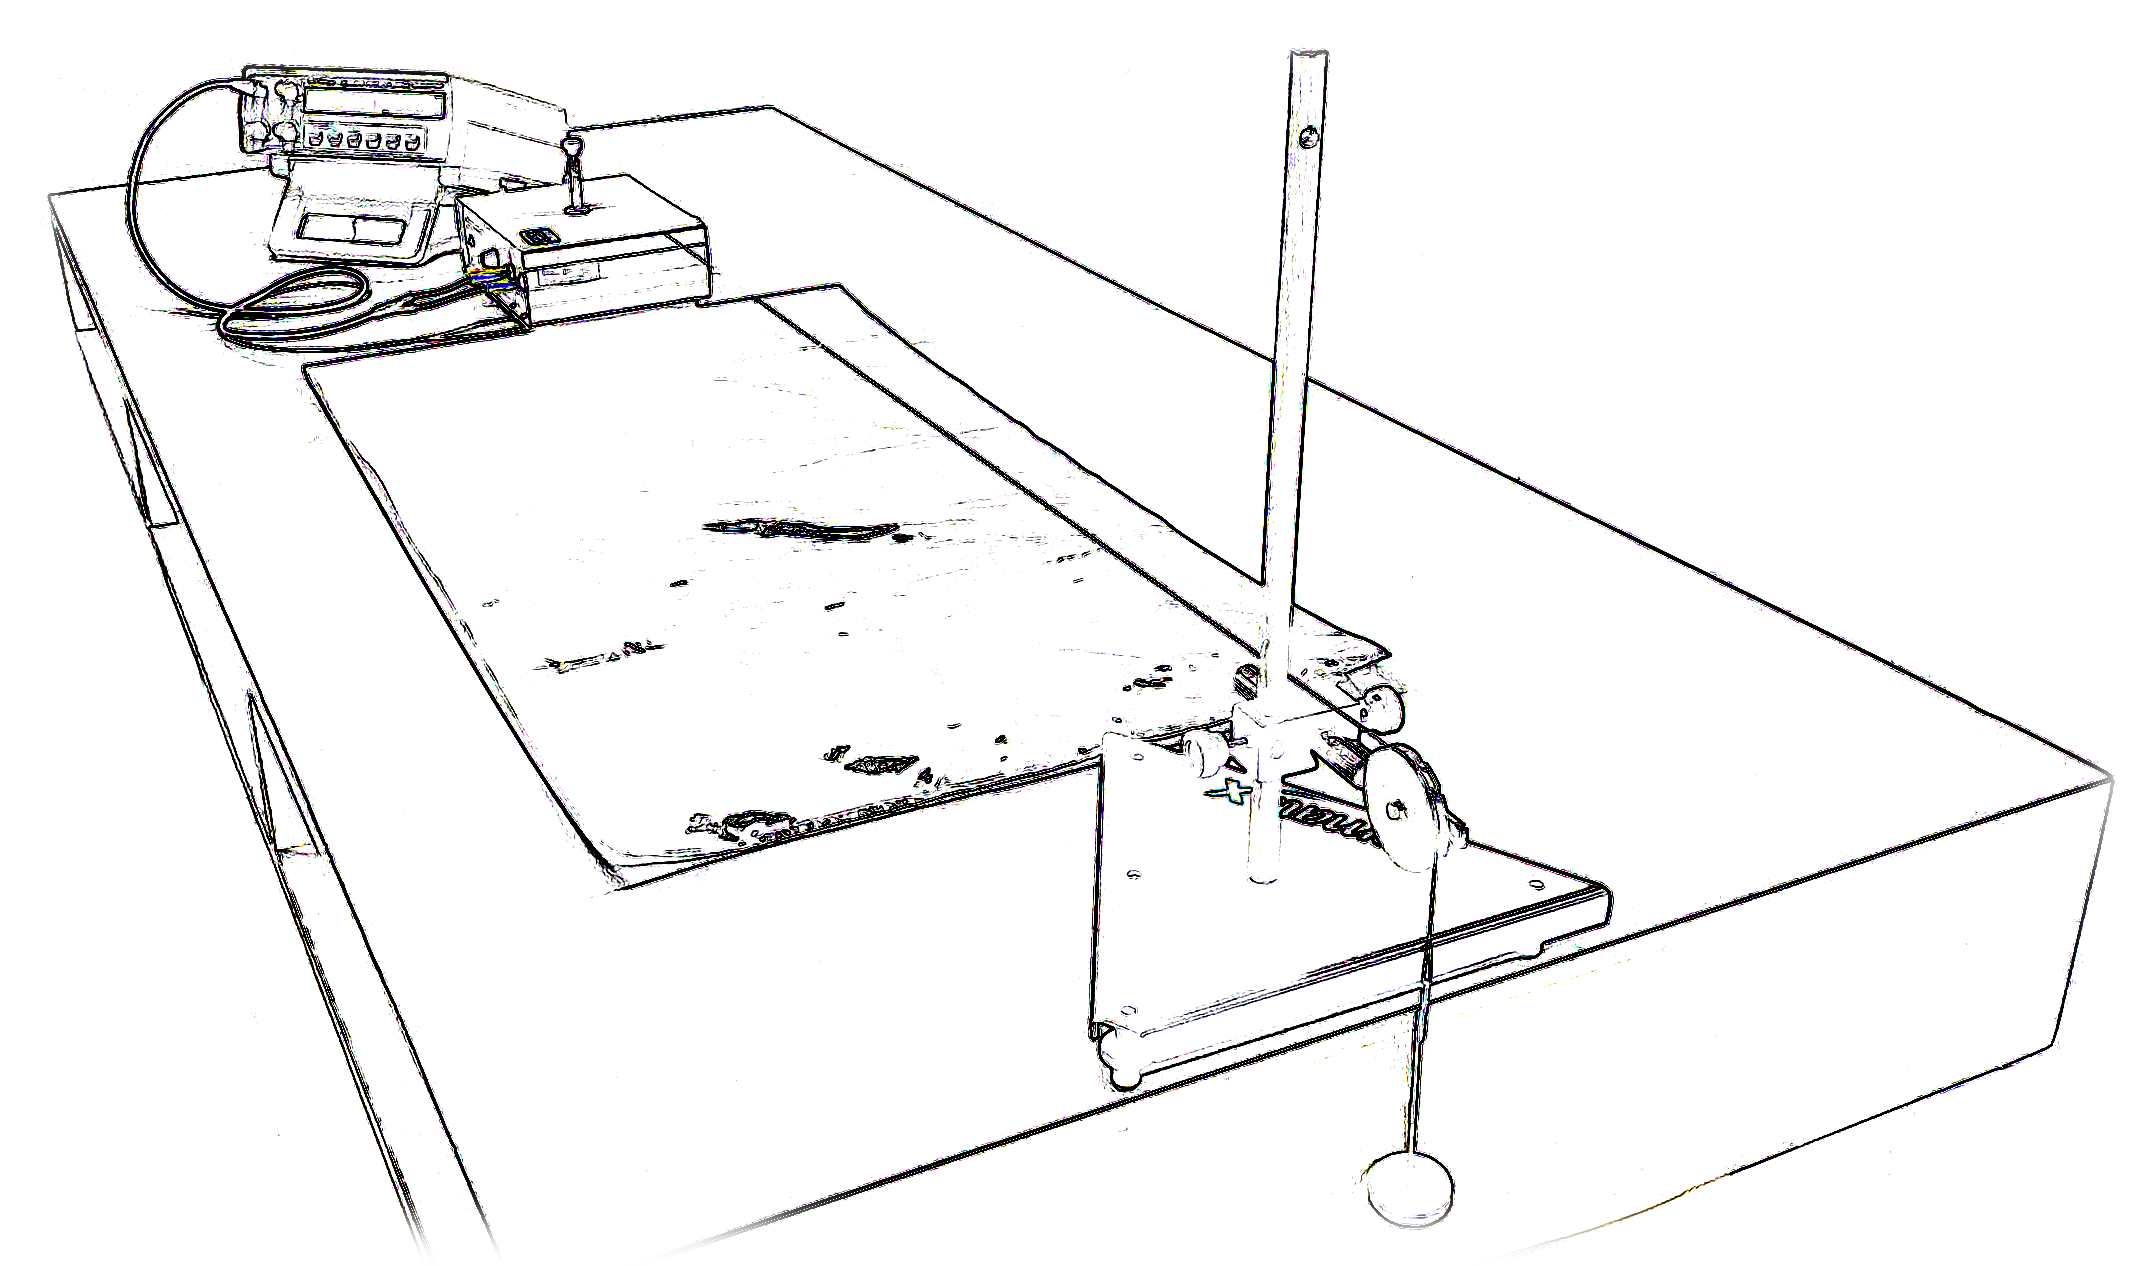
\includegraphics[width=\textwidth]{Ilustrations/Ondas_estacionarias.png}
	\caption{Aparato para a visualização de ondas estacionárias em uma corda.}
\end{figure}

%%%%%%%%%%%%%%%%%%%%%%%%%%%%%%%%%%%%%%%%%%%%%%%%%%%%%%%%%%%%%%%%%%%%%%%%%%%%%%%
\section{Material Necessário}
%%%%%%%%%%%%%%%%%%%%%%%%%%%%%%%%%%%%%%%%%%%%%%%%%%%%%%%%%%%%%%%%%%%%%%%%%%%%%%%

\begin{itemize}
	\item Gerador de ondas;
	\item Trena;
	\item Fio fino;
	\item Balança;
	\item Anilhas leves e gancho;
	\item Polia com suporte.
\end{itemize}

%%%%%%%%%%%%%%%%%%%%%%%%%%%%%%%%%%%%%%%%%%%%%%%%%%%%%%%%%%%%%%%%%%%%%%%%%%%%%%%
\section{Procedimento Experimental}
%%%%%%%%%%%%%%%%%%%%%%%%%%%%%%%%%%%%%%%%%%%%%%%%%%%%%%%%%%%%%%%%%%%%%%%%%%%%%%%

%%%%%%%%%%%%%%%%%%%%%%%%%%%%%%%%%%%%%%%%%%%%%%%%%%%%%%%%%%%%%%%%%%%%%%%%
\subsection{Determinação da densidade linear de massa do fio (opcional)}
%%%%%%%%%%%%%%%%%%%%%%%%%%%%%%%%%%%%%%%%%%%%%%%%%%%%%%%%%%%%%%%%%%%%%%%%

O valor de densidade de massa do fio utilizado pode ser determinado com a utilização de uma balança de alta precisão\footnote{Caso a determinação da densidade linear de massa $\mu$  não seja feita experimentalmente, utilize o valor de $\mu = (\np{9,010} \pm \np{0,002})\times 10^{-4} \rm{g/cm}$.} . Para isso basta tomarmos um segmento com um comprimento $L$ arbitrário, porém determinado, e verificarmos qual a massa $m$ correspondente. Obtemos a densidade linear de massa $\mu$ através da razão
\begin{equation}
	\mu = \frac{m}{L}.
\end{equation}
%
O valor obtido dessa forma será considerado o \emph{valor de referência} na análise de dados.

%%%%%%%%%%%%%%%%%%%%%%%%%%%%%%%%%%%%%%%%%%%%%%%%%%%%%%%%%%%%%%%%%%%%%%%%%%%
\subsection{Dependência da frequência de ressonância com a tensão aplicada}
%%%%%%%%%%%%%%%%%%%%%%%%%%%%%%%%%%%%%%%%%%%%%%%%%%%%%%%%%%%%%%%%%%%%%%%%%%%

\begin{enumerate}
\item Ligue o gerador de ondas ao oscilador eletromecânico, dispondo o segundo a uma distância de aproximadamente \np[m]{1,30} da extremidade da mesa;\label{Enum:iteminicio}
\item Prenda a polia ao suporte e a disponha de forma que fique para fora da mesa.
\item Tome um segmento de fio com tamanho adequado e o prenda ao pino do oscilador. Anote na Tabela~\ref{Tab:FrequenciaFuncaoMassa} o valor de referência para densidade linear de massa $\mu$ do fio utilizado;
\item Afira a massa do gancho, juntamente com uma anilha e os pendure na extremidade livre da corda, fazendo-a passar pela polia e deixando o gancho suspenso. Anote na Tabela~\ref{Tab:FrequenciaFuncaoMassa} o valor da massa $m$ suspensa na corda;\label{Enum:itemfim}
\item Ligue o gerador de ondas e varie a frequência até que se forme uma onda estacionária com dois\footnote{Esse harmônico foi escolhido por ser o de mais fácil visualização.} ventres ($n' =2$);
\item Anote o valor da frequência $f$ em que a onda estacionária se forma na Tabela~\ref{Tab:FrequenciaFuncaoMassa}. \emph{Obs.: Em alguns equipamentos, a frequência pode variar constantemente. Nesse caso, anote os valores com uma casa após a vírgula e adote o valor de erro como sendo \np[Hz]{0,1}.}
\item Utilize a trena/régua para medir a distância $L$ entre \emph{os nós das extremidades}\footnote{A distância deve ser medida entre o ponto em que a corda toca a polia (onde se localiza um dos nós) e o nó que deve se formar um pouco antes do pino do oscilador. Em muitos casos o nó se forma tão próximo do pino que não podemos distinguí-lo. Nesse caso meça a distância entre a polia e o próprio pino do oscilador. Este valor é, efetivamente, o comprimento da corda.}. Anote o valor obtido na Tabela~\ref{Tab:FrequenciaFuncaoMassa}. Esse valor será aproximadamente constante e não precisa ser medido novamente.
\item Adicione mais uma anilha ao gancho e repita o processo a partir do item \ref{Enum:itemfim} até que a tabela seja completamente preenchida.
\end{enumerate}

%%%%%%%%%%%%%%%%%%%%%%%%%%%%%%%%%%%%%%%%%%%%%%%%%%%%%%%%%%%%%%%%%%%%%%%%%%%%%%
\subsection{Dependência da frequência de ressonância com o comprimento do fio}
%%%%%%%%%%%%%%%%%%%%%%%%%%%%%%%%%%%%%%%%%%%%%%%%%%%%%%%%%%%%%%%%%%%%%%%%%%%%%%

\begin{enumerate}
\item Mantenha o aparato disposto conforme a descrição da seção anterior;
\item Utilizando uma ou duas anilhas, verifique o valor da massa $m$ suspensa pelo fio (gancho e anilhas) e anote na Tabela~\ref{Tab:FrequenciaFuncaoComprimento2}. Desta vez manteremos a massa constante. Anote também o valor de referência da densidade linear de massa $\mu$ do fio;
\item Ligue o gerador de ondas e varie a frequência até que se forme uma onda estacionária com dois ventres ($n' = 2$). Anote o valor de frequência $f$ na Tabela~\ref{Tab:FrequenciaFuncaoComprimento2};\label{Item:OndasEstSegParteLoop}
\item Utilize a trena para medir a distância $L$ entre \emph{os nós das extremidades}.\footnote{Novamente, devemos medir a distância entre o nó determinado pelo ponto em que a corda toca a polia e o nó que se forma próximo ao pino do oscilador.} Anote o valore de $L$ na Tabela~\ref{Tab:FrequenciaFuncaoComprimento2};
\item Mova o oscilador aproximadamente \np[cm]{10,0} em direção à polia e repita o processo a partir do item \ref{Item:OndasEstSegParteLoop} até preencher a tabela ou até que as anilhas estejam prestes a tocar o chão.
\item Repita os itens acima para ondas estacionárias com \emph{três ventres} ($n' = 3$), preenchendo a Tabela~\ref{Tab:FrequenciaFuncaoComprimento3}.
\end{enumerate}

%%%%%%%%%%%%%%%%%%%%%%%%%%%%%%%%%%%%%%%%%%%%%%%%%%%%%%%%%%%%%%%%%%%%%%%%%%%%%%%
%%%%%%%%%%%%%%%%%%%%%%%%%%%%%%%%%%%%%%%%%%%%%%%%%%%%%%%%%%%%%%%%%%%%%%%%%%%%%%%
%%%%%%%%%%%%%%%%%%%%%%%%%%%%%%%%%%%%%%%%%%%%%%%%%%%%%%%%%%%%%%%%%%%%%%%%%%%%%%%
%%%%%%%%%%%%%%%%%%%%%%%%%%%%%%%%%%%%%%%%%%%%%%%%%%%%%%%%%%%%%%%%%%%%%%%%%%%%%%%
\cleardoublepage

\noindent{}{\huge\textit{Ondas Estacionárias}}

\vspace{15mm}

\begin{fullwidth}
\noindent{}\makebox[0.6\linewidth]{Turma:\enspace\hrulefill}\makebox[0.4\textwidth]{  Data:\enspace\hrulefill}
\vspace{5mm}

\noindent{}\makebox[0.6\linewidth]{Aluno(a):\enspace\hrulefill}\makebox[0.4\textwidth]{  Matrícula:\enspace\hrulefill}

\noindent{}\makebox[0.6\linewidth]{Aluno(a):\enspace\hrulefill}\makebox[0.4\textwidth]{  Matrícula:\enspace\hrulefill}

\noindent{}\makebox[0.6\linewidth]{Aluno(a):\enspace\hrulefill}\makebox[0.4\textwidth]{  Matrícula:\enspace\hrulefill}

\noindent{}\makebox[0.6\linewidth]{Aluno(a):\enspace\hrulefill}\makebox[0.4\textwidth]{  Matrícula:\enspace\hrulefill}

\noindent{}\makebox[0.6\linewidth]{Aluno(a):\enspace\hrulefill}\makebox[0.4\textwidth]{  Matrícula:\enspace\hrulefill}
\end{fullwidth}

\vspace{5mm}

%%%%%%%%%%%%%%%%%%%%%%%%%%%%%%%%%%%%%%%%%%%%%%%%%%%%%%%%%%%%%%%%%%%%%%%%%%%%%%%
\section{Questionário}
%%%%%%%%%%%%%%%%%%%%%%%%%%%%%%%%%%%%%%%%%%%%%%%%%%%%%%%%%%%%%%%%%%%%%%%%%%%%%%%

\begin{question}[type={exam}]{1}
Apresente os resultados de maneira clara e organizada. Mostre os cálculos requisitados de maneira clara e sucinta, evidenciando o raciocínio desenvolvido.
\end{question}

\begin{question}[type={exam}]{0.5}
Liste os equipamentos utilizados. Para os instrumentos de medida, descreva o tipo do equipamento, sua resolução, e seu erro de escala.
\end{question}

\begin{question}[type={exam}]{0.5}
Preencha as tabelas com o número adequado de algarismos significativos, unidades, e erros de escala apropriados. 
\end{question}

\begin{question}[type={exam}]{1}\label{Q:Ondas:GraficoFM}
Elabore um gráfico \textbf{linear} de $f$ em função da massa $m$ para os dados da Tabela~\ref{Tab:FrequenciaFuncaoMassa}. \emph{Será necessário efetuar uma mudança de variáveis}.
\end{question}

\begin{question}[type={exam}]{1}\label{Q:Ondas:CoeficientesRetaFM}
Para a questão anterior, calcule a reta que melhor representa os dados experimentais utilizando o método dos mínimos quadrados e a adicione ao gráfico.
\end{question}

\begin{question}[type={exam}]{1}
Considerando a linearização adotada na Questão~\ref{Q:Ondas:GraficoFM} e a a Equação~\eqref{Eq:RelacaoVariaveisOndasEstacionarias}, identifique os coeficientes angular $B$ e linear $A$. Utilizando a relação obtida para o coeficiente angular, determine a densidade linear de massa do fio a partir do valor obtido para $B$ na questão anterior. Determine o erro percentual em relação ao valor de referência utilizando a expressão 
\begin{equation}
	E_{\%} = \left|\frac{x-x_{\textrm{ref}}}{x_{\textrm{ref}}}\right| \times 100.
\end{equation}
\end{question}

\begin{question}[type={exam}]{1.5}
Calcule o erro associado ao coeficiente angular obtido na Questão~\ref{Q:Ondas:CoeficientesRetaFM}. A partir dos valores do coeficiente e do erro, determine o erro associado à densidade linear de massa do fio.
\end{question}

\begin{question}[type={exam}]{1}
Elabore um gráfico\footnote{Os dois conjuntos de dados devem estar contidos no mesmo gráfico.} \textbf{linear} de $f$ em função de $L$ para os dados das Tabelas~\ref{Tab:FrequenciaFuncaoComprimento2} e~\ref{Tab:FrequenciaFuncaoComprimento3}. \emph{Novamente, será necessário efetuar uma mudança de variáveis}.
\end{question}

\begin{question}[type={exam}]{1}
Para a questão anterior, calcule as retas que melhor representam os dados experimentais utilizando o método dos mínimos quadrados e as adicione ao gráfico.
\end{question}

%\begin{question}[type={exam}]{1}
%Utilize a Equação~\eqref{Eq:RelacaoVariaveisOndasEstacionarias} para descrever a relação entre $f$ e $L$, identificando as variáveis dependente e independente, bem como os coeficientes angular e linear. A partir dos valores dos coeficientes angulares, determine os valores da aceleração da gravidade para cada conjunto de dados. Determine o erro percentual em relação ao valor de referência utilizando a expressão 
%\begin{equation}
%	E_{\%} = \left|\frac{x-x_{\textrm{ref}}}{x_{\textrm{ref}}}\right| \times 100.
%\end{equation}
%\end{question}

%\begin{question}[type={exam}]{1}
%Calcule o erro associado ao coeficiente angular obtido na questão anterior para a regressão linear dos dados da Tabela~\ref{Tab:FrequenciaFuncaoComprimento2}. Com esse resultado e com o valor do próprio coeficiente angular, determine o valor do erro associado à aceleração da gravidade. Nos cálculos, use o valor de $\mu$ de referência (incluindo o erro erro associado).
%\end{question}

\begin{question}[type={exam}]{1.5}
Considerando os objetivos do experimento, listados na Seção~\ref{Sec:ObjetivosOndasEstacionarias}, e os resultados obtidos nas questões anteriores, discuta quais objetivos foram atingidos com sucesso, justificando suas conclusões. Se algum objetivo não foi atingido, discuta quais são os possíveis motivos do fracasso e que providências podem ser tomadas para que eles sejam alcançados.
\end{question}

\clearpage
%%%%%%%%%%%%%%%%%%%%%%%%%%%%%%%%%%%%%%%%%%%%%%%%%%%%%%%%%%%%%%%%%%%%%%%%%%%%%%%
\section{Tabelas}
%%%%%%%%%%%%%%%%%%%%%%%%%%%%%%%%%%%%%%%%%%%%%%%%%%%%%%%%%%%%%%%%%%%%%%%%%%%%%%%

\begin{table}[!htb]
\caption{Dados para a frequência de surgimento do \textbf{segundo harmônico} ($n' = 2$).}
\label{Tab:FrequenciaFuncaoMassa}
	\begin{center}
		\begin{tabular}{cp{45mm}p{45mm}c}
		\toprule
\multicolumn{2}{l}{\textbf{Parâmetros constantes}}&&\\
		\cmidrule{2-3}
		& \cellcolor[gray]{0.89}$L$ &\cellcolor[gray]{0.92} \\
		& \cellcolor[gray]{0.95}$\mu$ & \cellcolor[gray]{0.97}\\
		\cmidrule{2-3}
		\\
\multicolumn{3}{l}{\textbf{Dados para a massa e a frequência correspondente}} \\
		\cmidrule{2-3}		
		& $m$ & $f$ \\
		\cmidrule{2-3}
		& \cellcolor[gray]{0.89} & \cellcolor[gray]{0.92} \\
		& \cellcolor[gray]{0.95} & \cellcolor[gray]{0.97} \\
		& \cellcolor[gray]{0.89} & \cellcolor[gray]{0.92} \\
		& \cellcolor[gray]{0.95} & \cellcolor[gray]{0.97} \\
		& \cellcolor[gray]{0.89} & \cellcolor[gray]{0.92} \\
		& \cellcolor[gray]{0.95} & \cellcolor[gray]{0.97} \\
		& \cellcolor[gray]{0.89} & \cellcolor[gray]{0.92} \\
		& \cellcolor[gray]{0.95} & \cellcolor[gray]{0.97} \\
		\cmidrule{2-3}		
		\bottomrule
		\end{tabular}
	\end{center}
\end{table}

%\begin{table}[!htb]
%\forcerectofloat
%\caption{Dados para a frequência de surgimento do \textbf{primeiro harmônico} ($n' = 1$).}
%\label{Tab:FrequenciaFuncaoComprimento1}
%	\begin{center}
%		\begin{tabular}{cp{45mm}p{45mm}c}
%		\toprule
%\multicolumn{2}{l}{\textbf{Parâmetros constantes}}&\\
%		\cmidrule{2-3}
%		& \cellcolor[gray]{0.89}$m$ &\cellcolor[gray]{0.92} \\
%		& \cellcolor[gray]{0.95}$\mu$ & \cellcolor[gray]{0.97}\\
%		\cmidrule{2-3}
%		\\
%\multicolumn{3}{l}{\textbf{Dados para a comprimento e a frequência correspondente}} \\
%		\cmidrule{2-3}		
%		& $L$ & $f$ &\\
%		\cmidrule{2-3}
%		& \cellcolor[gray]{0.89} & \cellcolor[gray]{0.92} \\
%		& \cellcolor[gray]{0.95} & \cellcolor[gray]{0.97} \\
%		& \cellcolor[gray]{0.89} & \cellcolor[gray]{0.92} \\
%		& \cellcolor[gray]{0.95} & \cellcolor[gray]{0.97} \\
%		& \cellcolor[gray]{0.89} & \cellcolor[gray]{0.92} \\
%		& \cellcolor[gray]{0.95} & \cellcolor[gray]{0.97} \\
%		& \cellcolor[gray]{0.89} & \cellcolor[gray]{0.92} \\
%		& \cellcolor[gray]{0.95} & \cellcolor[gray]{0.97} \\
%		\cmidrule{2-3}
%		\bottomrule
%		\end{tabular}
%	\end{center}
%\end{table}

\begin{table}[!htb]
\forcerectofloat
\caption{Dados para a frequência de surgimento do \textbf{segundo harmônico} ($n' = 2$).}
\label{Tab:FrequenciaFuncaoComprimento2}
	\begin{center}
		\begin{tabular}{cp{45mm}p{45mm}c}
		\toprule
\multicolumn{2}{l}{\textbf{Parâmetros constantes}}&\\
		\cmidrule{2-3}
		& \cellcolor[gray]{0.89}$m$ &\cellcolor[gray]{0.92} \\
		& \cellcolor[gray]{0.95}$\mu$ & \cellcolor[gray]{0.97}\\
		\cmidrule{2-3}
		\\
\multicolumn{3}{l}{\textbf{Dados para a comprimento e a frequência correspondente}} \\
		\cmidrule{2-3}		
		& $L$ & $f$ &\\
		\cmidrule{2-3}
		& \cellcolor[gray]{0.89} & \cellcolor[gray]{0.92} \\
		& \cellcolor[gray]{0.95} & \cellcolor[gray]{0.97} \\
		& \cellcolor[gray]{0.89} & \cellcolor[gray]{0.92} \\
		& \cellcolor[gray]{0.95} & \cellcolor[gray]{0.97} \\
		& \cellcolor[gray]{0.89} & \cellcolor[gray]{0.92} \\
		& \cellcolor[gray]{0.95} & \cellcolor[gray]{0.97} \\
		& \cellcolor[gray]{0.89} & \cellcolor[gray]{0.92} \\
		& \cellcolor[gray]{0.95} & \cellcolor[gray]{0.97} \\
		\cmidrule{2-3}
		\bottomrule
		\end{tabular}
	\end{center}
\end{table}

\begin{table}[!htb]
\forceversofloat
\caption{Dados para a frequência de surgimento do \textbf{terceiro harmônico} ($n' = 3$).}
\label{Tab:FrequenciaFuncaoComprimento3}
	\begin{center}
		\begin{tabular}{cp{45mm}p{45mm}c}
		\toprule
\multicolumn{2}{l}{\textbf{Parâmetros constantes}}&\\
		\cmidrule{2-3}
		& \cellcolor[gray]{0.89}$m$ &\cellcolor[gray]{0.92} \\
		& \cellcolor[gray]{0.95}$\mu$ & \cellcolor[gray]{0.97}\\
		\cmidrule{2-3}
		\\
\multicolumn{3}{l}{\textbf{Dados para a comprimento e a frequência correspondente}} \\
		\cmidrule{2-3}		
		& $L$ & $f$ &\\
		\cmidrule{2-3}
		& \cellcolor[gray]{0.89} & \cellcolor[gray]{0.92} \\
		& \cellcolor[gray]{0.95} & \cellcolor[gray]{0.97} \\
		& \cellcolor[gray]{0.89} & \cellcolor[gray]{0.92} \\
		& \cellcolor[gray]{0.95} & \cellcolor[gray]{0.97} \\
		& \cellcolor[gray]{0.89} & \cellcolor[gray]{0.92} \\
		& \cellcolor[gray]{0.95} & \cellcolor[gray]{0.97} \\
		& \cellcolor[gray]{0.89} & \cellcolor[gray]{0.92} \\
		& \cellcolor[gray]{0.95} & \cellcolor[gray]{0.97} \\
		\cmidrule{2-3}
		\bottomrule
		\end{tabular}
	\end{center}
\end{table}


%%%%%%%%%%%%%%%%%%%%%%%%%%%%%%%%%%%%%%%%%%%%%%%%%%%%%%%%%%%%%%%%%%%%%%%%%%%%%%%
\chapter{Dilatação linear e lei de resfriamento de Newton}
\label{Chap:ExpDilatacaoLinear}
%%%%%%%%%%%%%%%%%%%%%%%%%%%%%%%%%%%%%%%%%%%%%%%%%%%%%%%%%%%%%%%%%%%%%%%%%%%%%%%

\begin{fullwidth}\it
	Realizaremos um experimento de dilatação linear de sólidos verificando a relação entre o comprimento de tubos metálicos e sua temperatura. Verificaremos também qual é a evolução temporal da temperatura dos tubos no processo de resfriamento. A partir dos resultados obtidos, calcularemos os coeficientes de dilatação dos materiais dos tubos e os identificaremos. Verificaremos também qual é a expressão que descreve a evolução da temperatura durante o processo de resfriamento. Veremos a expressão para a dilatação linear e também o conceito de equação diferencial. Utilizaremos os seguintes conceitos/técnicas de análise de dados: medidas, algarismos significativos, gráficos, software para elaboração de gráficos, erros de escala e propagados, equação geral para o erro propagado, regressão linear, linearização, e erros dos coeficientes $A$ e $B$.
\end{fullwidth}

%%%%%%%%%%%%%%%%%%%%%%%%%%%%%%%%%%%%%%%%%%%%%%%%%%%%%%%%%%%%%%%%%%%%%%%%%%%%%%%
\section{Dilatação Linear}
%%%%%%%%%%%%%%%%%%%%%%%%%%%%%%%%%%%%%%%%%%%%%%%%%%%%%%%%%%%%%%%%%%%%%%%%%%%%%%%

Ao resfriarmos ou aquecermos um objeto, vericamos que ele tem suas dimensões alteradas. Isso é especialmente notável em fios longos, pois a variação do comprimento é proporcional ao comprimento do objeto. Esse fenômeno têm muitas implicações práticas: pontes necessitam de juntas de dilatação, assim como pisos e trilhos de trem. Caso não as tivessem, com um aumento ou diminuição de temperatura, apareceriam deformações e rachaduras que deteriorariam essas estruturas. 

Muitas vezes esse tipo de comportamento pode ser usado de maneira positiva: duas peças metálicas podem ser unidas sem soldas se elas forem feitas de forma que uma das peças encaixe em um orifício da outra somente se a segunda for aquecida ---~estando, portanto, dilatada~---. Quando a peça externa for resfriada, ela se contrairá e acabará prendendo a peça interna.

Além de notarmos que a dilatação é proporcional às dimensões do objeto, verifica-se experimentalmente que quanto maior a variação de temperatura a que o objeto é submetido, maior é a variação do comprimento. Observamos ainda que materiais diferentes tem variações diferentes de comprimento para uma mesma variação de temperatura. Essas observações podem ser condensadas na seguinte equação:
\begin{equation}
	\Delta L = L_0\alpha\Delta T,
\end{equation}
%
onde $\alpha$ é uma constante característica do material, $L_0$ é o comprimento inicial do objeto --- ou seja, seu comprimento antes de sofrer a variação de temperatura --- e $\Delta T = T - T_0$ ($T_0$ é a temperatura inicial e $T$ é a temperatura final do corpo). 

Se compararmos a expressão acima com a equação da reta $y = A + Bx$, podemos fazer a seguinte identificação entre as variáveis:
\begin{align*}
	y &= \Delta L & x &= (T - T_0)\\
	A &= 0 & B &= \alpha L_0
\end{align*}

\begin{margintable}
\centering
\begin{tabular}{cc}
\toprule
Material & $\alpha$ ($\nicefrac{1}{\tcdegree\textrm{C}}$) \\
\midrule
  Alumínio & \np{23,1e-6} \\
  Bronze/Latão & \np{19e-6} \\
  Cobre & \np{16,5e-6} \\
  Chumbo & \np{28,9e-6} \\
  Ferro & \np{11,8e-6} \\
  Aço & \np{11e-6} \\
\bottomrule
\end{tabular}
\vspace{1mm}
\caption{Valores dos coeficientes de expansão térmica para alguns metais.}
\label{TabelaCoeficientes}
\end{margintable}

\noindent{}Segundo as relações acima, se realizarmos um experimento no qual variamos a temperatura de --- por exemplo --- uma barra metálica, anotando os valores do variação do comprimento em função da variação de temperatura, verificaremos ao fazer a regressão linear que o coeficiente angular $B$ será igual ao produto do coeficiente de expansão térmica $\alpha$ pelo comprimento inicial da barra.

\begin{figure}
\centering
\forceversofloat
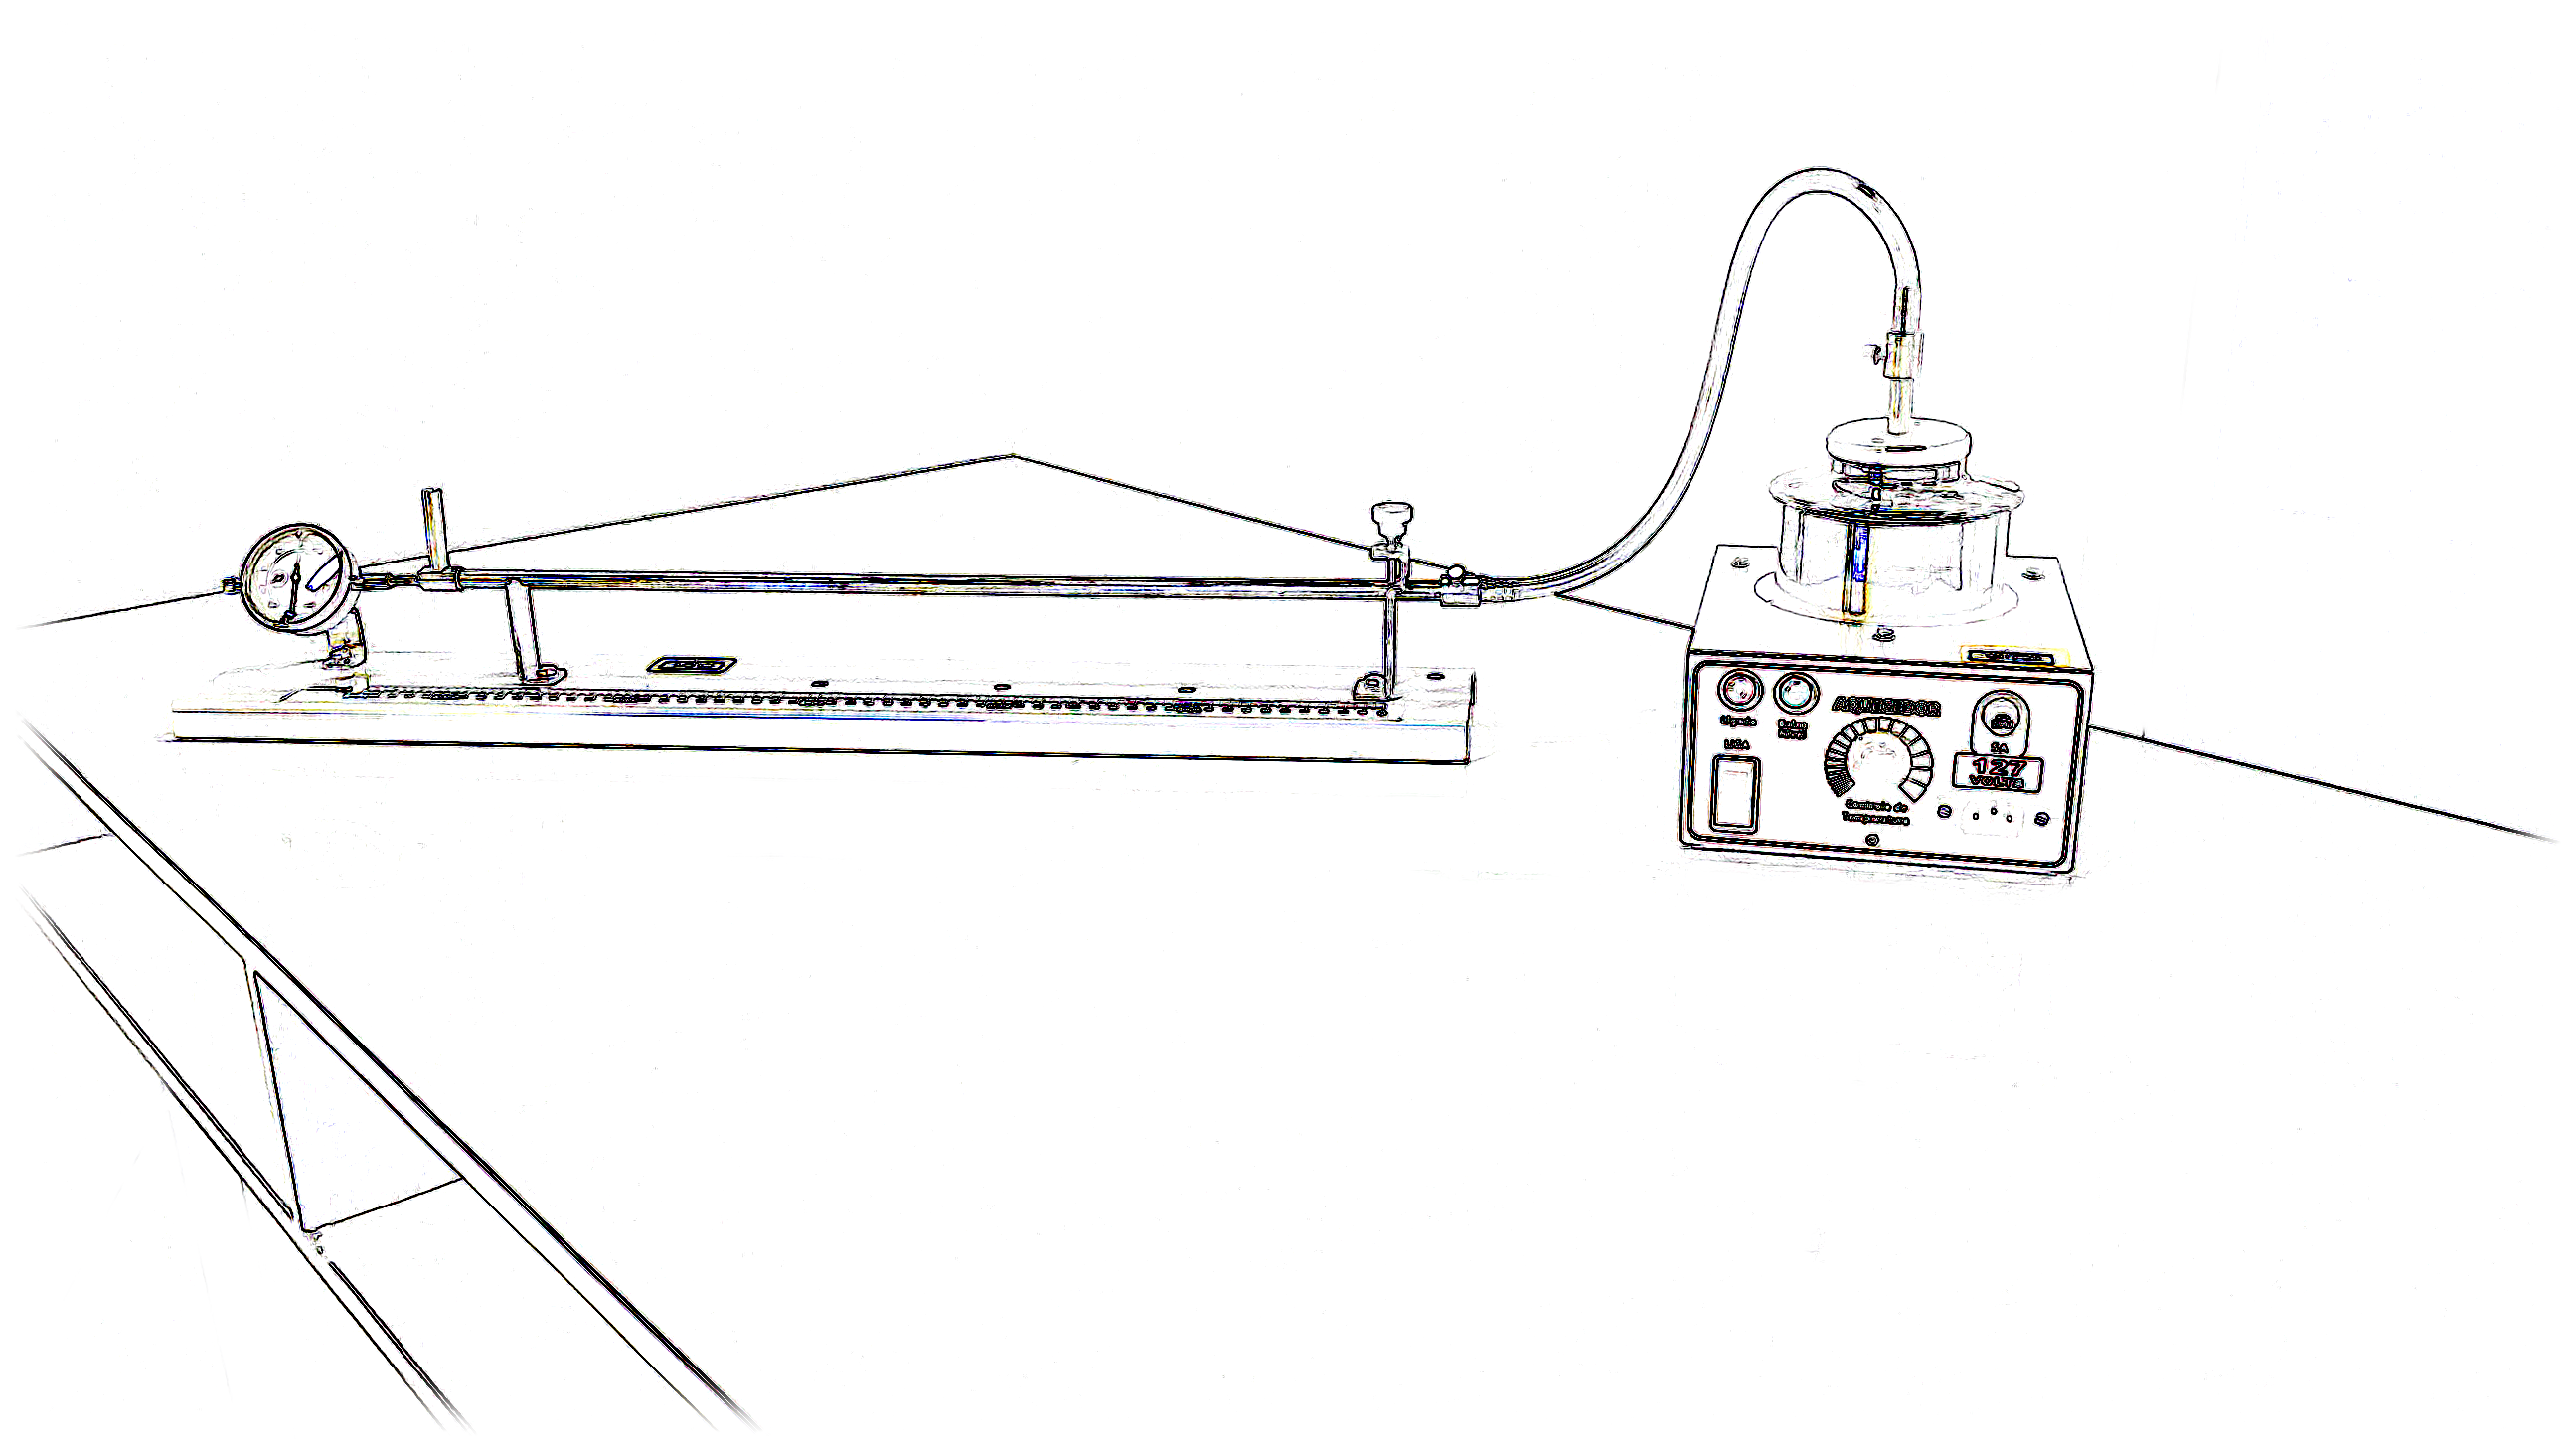
\includegraphics[width=\textwidth]{Ilustrations/Dilatacao.png}
\caption{Equipamento para a verificação experimental da dilatação linear de sólidos.}
\end{figure}
%%%%%%%%%%%%%%%%%%%%%%%%%%%%%%%%%%%%%%%%%%%%%%%%%%%%%%%%%%%%%%%%%%%%%%%%%%%%%%%
\section{Lei de resfriamento de Newton}
%%%%%%%%%%%%%%%%%%%%%%%%%%%%%%%%%%%%%%%%%%%%%%%%%%%%%%%%%%%%%%%%%%%%%%%%%%%%%%%
% Caso especial da equação de Fourier para a condução de calor

De acordo com a lei do resfriamento de Newton\footnote{\url{http://www.ugrad.math.ubc.ca/coursedoc/math100/notes/diffeqs/cool.html}}
\begin{quote}\it
	A taxa de variação da temperatura de um corpo é proporcional à diferença entre sua temperatura e a temperatura do ambiente.
\end{quote}
%
Em termos matemáticos podemos descrever a afirmação acima como
\begin{equation}
	\frac{dT}{dt} \propto -(T - T_a),
\end{equation}
%
onde $T$ representa a temperatura do corpo, $dT/dt$ representa a taxa de variação temporal de tal temperatura e $T_a$ representa a temperatura ambiente. O sinal negativo denota o fato de que se $T > T_a$, o corpo sofre uma \emph{diminuição} de sua temperatura, o que significa que $dT/dt < 0$. Podemos escrever a equação acima como uma igualdade com o auxílio de uma constante:
\begin{equation}\label{Eq:VarTIgualKT}
	\frac{dT}{dt} = -k (T - T_a).
\end{equation}

Verificamos que a temperatura $T$ deve ser então uma \emph{função do tempo}, ou seja $T = T(t)$. Podemos encontrar tal função se definirmos
\begin{equation}
	y(t) = T(t) - T_a,
\end{equation}
%
de onde temos que
\begin{equation}
	\frac{dy(t)}{dt} = \frac{dT(t)}{dt} - \frac{dT_a}{dt}.
\end{equation}
%
O segundo termo à direita é zero, pois a temperatura ambiente é constante, portanto
\begin{equation}
	\frac{dy(t)}{dt} = \frac{dT(t)}{dt}.
\end{equation}
%
Substituindo esse resultado e a própria definição de $y(t)$ na Equação~\ref{Eq:VarTIgualKT}, obtemos
\begin{equation}
	\frac{dy(t)}{dt} = -ky(t),
\end{equation}
%
o que pode ser reescrito como
\begin{equation}
	\frac{dy(t)}{y(t)} = -k dt.
\end{equation}

Se imaginarmos que $y(t)$ tem um valor inicial $y(t_i)$ no instante $t_i$ e um valor final $y(t_f)$ em um instante $t_f$, podemos integrar o lado esquerdo entre os valores inicial e final de $y(t)$ e o lado direito entre os valores inicial e final do tempo, obtendo
\begin{equation}
	\int_{y(t_i)}^{y(t_f)} \frac{dy(t)}{y(t)} = -k \int_{t_i}^{t_f} dt,
\end{equation}
%
o que resulta em
\begin{equation}\label{Eq:TempFuncTempoLN}
	\ln \frac{y(t_f)}{y(t_i)} = - k (t_f - t_i),
\end{equation}
%
onde usamos $\ln \alpha - \ln \beta = \ln (\alpha/\beta)$. Essa equação fica mais simples se fizermos $t_i = 0$, $t_f = t$ e tomarmos a exponencial de ambos os lados da equação:
\begin{equation}
	y(t) = y(0) e^{-kt}.
\end{equation}
%
Finalmente, se notarmos que $y(0) = T(0) - T_a$ e que $T(0)$ é a temperatura inicial $T_0$ do corpo, encontramos
\begin{equation}
	T(t) = T_a + (T_0 - T_a)e^{-kt}.
\end{equation}
%
Temos então que a temperatura do corpo decai segundo uma lei \emph{exponencial}, com uma constante característica $k$.
%
\begin{marginfigure}
\centering
\begin{tikzpicture}[>=Stealth,domain=0:4.3]
	\draw[->] (0,0) -- (4.5,0) node[below]{$t$};
	\draw[->] (0,0) -- (0,3.5) node[left]{$T$};
	
	\draw[dashed] (0,1.2) node[left]{$T_a$} -- (4.3,1.2);
	
	\draw[smooth] plot (\x,{1.2 + (2.8 - 1.2) * exp(-0.5 *\x)});
	\draw[smooth] plot (\x,{1.2 + (0.8 - 1.2) * exp(-0.5 *\x)});
	
	\draw (0,2.8) node[left]{$T_1$};
	\draw (0,0.8) node[left]{$T_2$};
\end{tikzpicture}
\caption{Gráfico da temperatura em função do tempo para o resfriamento e para o aquecimento de um corpo segundo a Lei de Newton para o Resfriamento. As temperaturas iniciais são tais que $T_1 > T_a > T_2$, sendo que para $t\to\infty$ as temperaturas $T_1$ e $T_2$ tendem à temperatura ambiente.}
\end{marginfigure}

%%%%%%%%%%%%%%%%%%%%%%%%%
\subsection{Linearização}
%%%%%%%%%%%%%%%%%%%%%%%%%

Voltando à Equação~\ref{Eq:TempFuncTempoLN}, podemos reescrevê-la como
\begin{equation}
	\ln y(t) = -kt + \ln y(0)
\end{equation}
%
onde utilizamos $t_i = 0$. Utilizando a definição de $y(t)$, temos
\begin{equation}
	\ln (T(t) - T_a) = - kt + \ln(T_0 - T_a).
\end{equation}
%
Comparando essa equação com a equação da reta, temos
\begin{subequations}\label{Eq:LinResfriamentoNewton}
\begin{align}
	y &= \ln (T(t) - T_a) \\
	x &= t \\
	B &= -k \\
	A &= \ln(T_0 - T_a).
\end{align}
\end{subequations}
%
Portanto, podemos determinar o valor de $k$ a partir de uma regressão linear.

%%%%%%%%%%%%%%%%%%%%%%%%%%%%%%%%%%%%%%%%%%%%%%%%%%%%%%%%%%%%%%%%%%%%%%%%%%%%%%%
\section{Experimento}
%%%%%%%%%%%%%%%%%%%%%%%%%%%%%%%%%%%%%%%%%%%%%%%%%%%%%%%%%%%%%%%%%%%%%%%%%%%%%%%

Vamos aquecer tubos metálicos em forma de L através de um fluxo de vapor d'água. Como o tubo estará preso próximo da extremidade de sua lateral maior, verificaremos uma leitura no dilatômetro disposto em contato com a extremidade livre. Após isso, cessaremos o fluxo de vapor, permitindo que o tubo inicie um processo de resfriamento. Durante o resfriamento, monitoraremos a leitura do dilatômetro, que registrará o encolhimento do tubo, bem como de sua temperatura.

%%%%%%%%%%%%%%%%%%%%%%
\subsection{Objetivos}
\label{Sec:ObjetivosDilatacaoLinear}
%%%%%%%%%%%%%%%%%%%%%%

\begin{enumerate}
	\item Verificar a lineariedade da relação entre o comprimento de barras metálicas de diferentes materiais e a variação da temperatura.
	\item Calcular o coeficiente de expansão térmica para o material das barras identificando o material da barra com base em tal propriedade.
	\item Verificar o decaimento exponencial da temperatura, de acordo com a lei do resfriamento de Newton.
	\item Determinar o valor de $k$ para cada uma das barras.
\end{enumerate}

%%%%%%%%%%%%%%%%%%%%%%%%%%%%%%%%%%%%%%%%%%%%%%%%%%%%%%%%%%%%%%%%%%%%%%%%%%%%%%%
\section{Material Necessário}
%%%%%%%%%%%%%%%%%%%%%%%%%%%%%%%%%%%%%%%%%%%%%%%%%%%%%%%%%%%%%%%%%%%%%%%%%%%%%%%

\begin{itemize}
	\item Tubos metálicos em forma de L;
	\item Aquecedor elétrico de água;
	\item Termômetro;
	\item Régua;
	\item Aparato para medição de dilatações térmicas lineares;
	\item Cronômetro.
\end{itemize}

%%%%%%%%%%%%%%%%%%%%%%%%%%%%%%%%%%%%%%%%%%%%%%%%%%%%%%%%%%%%%%%%%%%%%%%%%%%%%%%
\section{Procedimento Experimental}
%%%%%%%%%%%%%%%%%%%%%%%%%%%%%%%%%%%%%%%%%%%%%%%%%%%%%%%%%%%%%%%%%%%%%%%%%%%%%%%
\begin{marginfigure}
	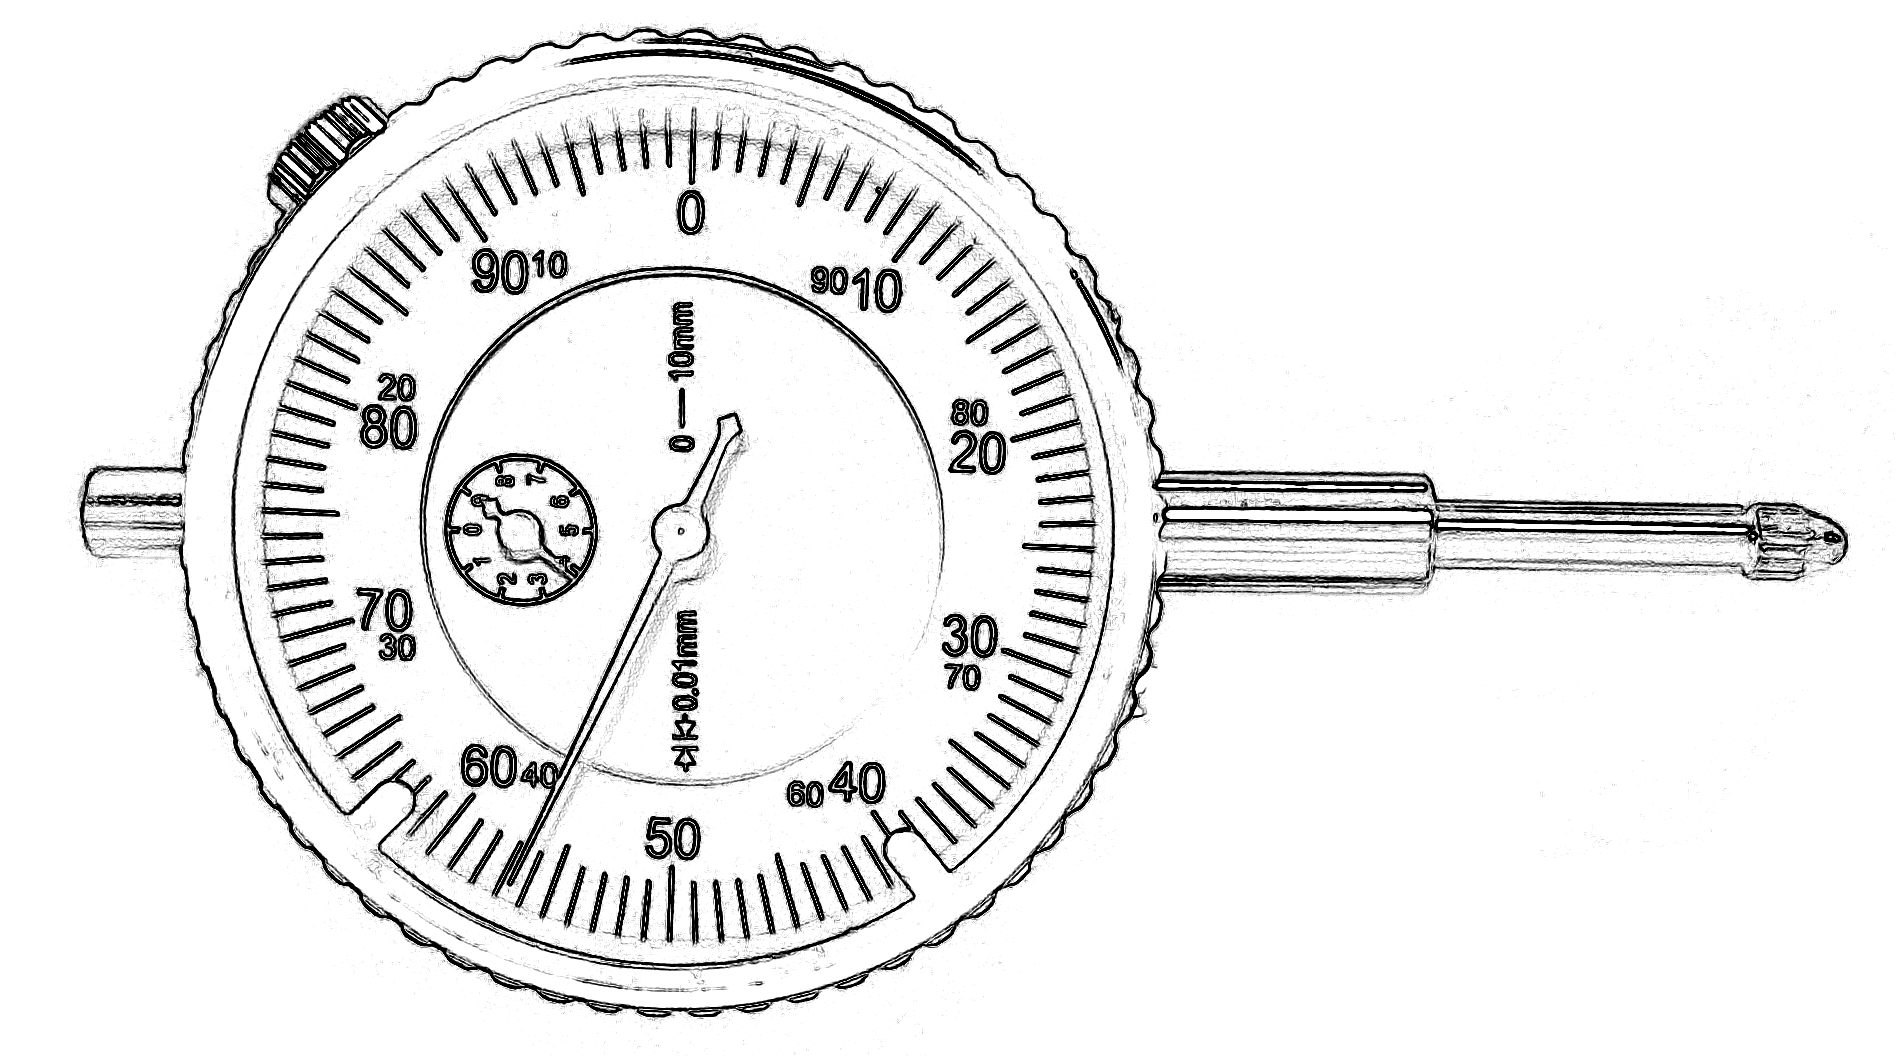
\includegraphics[width=\textwidth]{Ilustrations/Dilatometro.png}
	\caption{Dilatômetro. Note a existência de números pequenos para facilitar a leitura nos casos em que ocorre uma diminuição de tamanho. A coroa externa pode ser girada para zerar o dilatômetro, bastando para isso soltar o parafuso superior.}
\end{marginfigure}

\begin{enumerate}
\item Escolha um dos tubos metálicos e o coloque com a extremidade em forma de L em contato com o dilatômetro, com o segmento menor disposto verticalmente para cima.
\item Posicione a extremidade do tubo de forma que ela pressione o pino do dilatômetro e fique a uma distância de aproximadamente \np[mm]{520,0} do parafuso de fixação (utilize a escala milimetrada do suporte). Prenda a outra extremidade do tubo utilizando o parafuso do suporte.
\item Prenda a mangueira do aquecedor à extremidade horizontal do tubo (aquela oposta ao dilatômetro).
\item Adicione água ao aquecedor até uma profundidade de aproximadamente \np[cm]{5,0}. \emph{Importante: o aquecedor não pode ficar sem água durante o experimento, pois isso pode causar um superaquecimento e a consequente queima do aparelho.}
\item Ligue o aquecedor e aguarde  até que a água ferva.
\item Quando a água ferver, o tubo dilatará. Quando ele parar de dilatar, coloque o termômetro na extremidade do tubo mais próxima do dilatômetro e aguarde até que sua temperatura pare de variar.
\item Utilizando a régua ou a escala do suporte, meça o comprimento $L_0$ da barra entre o parafuso de fixação e a extremidade próxima ao dilatômetro. Anote este valor na Tabela~\ref{Tab:DadosTubo1}.
\item Anote também a temperatura $T_0$ indicada pelo termômetro.
\item Zere o dilatômetro girando a coroa exterior.
\item Zere o cronômetro.
\item Desligue o aquecedor e aguarde até que o ponteiro do dilatômetro passe a se mover\footnote{Veja que o dilatômetro sofre uma variação negativa, pois a barra está encolhendo. Faça a leitura nos números pequenos do mostrador.}. Assim que ele o fizer, inicie o cronômetro.
\item Quando a temperatura atingir \np[\tcdegree]{80}, faça a leitura do dilatômetro e do cronômetro e anote na Tabela~\ref{Tab:DadosTubo1}.
\item Faça a leitura do dilatômetro e do cronômetro a cada \np[\tcdegree C]{5,0} perdidos. Anote os valores na Tabela~\ref{Tab:DadosTubo1}, incluindo a temperatura. Cesse a leitura quando a temperatura do tubo estiver a aproximadamente \np[\tcdegree]{15,0} acima da temperatura ambiente.
\item Repita o procedimento para outro tubo e anote os dados na Tabela~\ref{Tab:DadosTubo2}.
\end{enumerate}

%%%%%%%%%%%%%%%%%%%%%%%%%%%%%%%%%%%%%%%%%%%%%%%%%%%%%%%%%%%%%%%%%%%%%%%%%%%%%%%
%%%%%%%%%%%%%%%%%%%%%%%%%%%%%%%%%%%%%%%%%%%%%%%%%%%%%%%%%%%%%%%%%%%%%%%%%%%%%%%
%%%%%%%%%%%%%%%%%%%%%%%%%%%%%%%%%%%%%%%%%%%%%%%%%%%%%%%%%%%%%%%%%%%%%%%%%%%%%%%
%%%%%%%%%%%%%%%%%%%%%%%%%%%%%%%%%%%%%%%%%%%%%%%%%%%%%%%%%%%%%%%%%%%%%%%%%%%%%%%
\cleardoublepage

\noindent{}{\huge\textit{Dilatação linear e lei de resfriamento de Newton}}

\vspace{15mm}

\begin{fullwidth}
\noindent{}\makebox[0.6\linewidth]{Turma:\enspace\hrulefill}\makebox[0.4\textwidth]{  Data:\enspace\hrulefill}
\vspace{5mm}

\noindent{}\makebox[0.6\linewidth]{Aluno(a):\enspace\hrulefill}\makebox[0.4\textwidth]{  Matrícula:\enspace\hrulefill}

\noindent{}\makebox[0.6\linewidth]{Aluno(a):\enspace\hrulefill}\makebox[0.4\textwidth]{  Matrícula:\enspace\hrulefill}

\noindent{}\makebox[0.6\linewidth]{Aluno(a):\enspace\hrulefill}\makebox[0.4\textwidth]{  Matrícula:\enspace\hrulefill}

\noindent{}\makebox[0.6\linewidth]{Aluno(a):\enspace\hrulefill}\makebox[0.4\textwidth]{  Matrícula:\enspace\hrulefill}

\noindent{}\makebox[0.6\linewidth]{Aluno(a):\enspace\hrulefill}\makebox[0.4\textwidth]{  Matrícula:\enspace\hrulefill}
\end{fullwidth}

\vspace{5mm}

%%%%%%%%%%%%%%%%%%%%%%%%%%%%%%%%%%%%%%%%%%%%%%%%%%%%%%%%%%%%%%%%%%%%%%%%%%%%%%%
\section{Questionário}
%%%%%%%%%%%%%%%%%%%%%%%%%%%%%%%%%%%%%%%%%%%%%%%%%%%%%%%%%%%%%%%%%%%%%%%%%%%%%%%

\begin{question}[type={exam}]{1}
Liste os instrumentos de medida utilizados. Descreva o tipo do equipamento, sua resolução, e seu erro de escala.
\end{question}

\begin{question}[type={exam}]{2}
Preencha as tabelas com o número adequado de algarismos significativos, unidades, e erros de escala apropriados. 
\end{question}

\begin{question}[type={exam}]{1.5}
\begin{enumerate}[label=\roman*.]
\item Elabore um gráfico\footnote{Os dois conjuntos de dados devem ser representados no mesmo gráfico, possibilitando a comparação entre eles. Note ainda que o gráfico será decrescente, uma vez que estamos verificando o processo de encolhimento das barras conforme elas resfriam.} de $|\Delta L| \times |T - T_0|$ com os dados das Tabelas~\ref{Tab:DadosTubo1} e~ \ref{Tab:DadosTubo2}.

\item Calcule as retas que melhor representam os dados experimentais utilizando o método dos mínimos quadrados e as adicione ao gráfico.
\item Utilizando os coeficientes angulares, obtenha o valor do coeficiente de expansão térmica e determine o erro percentual em comparação aos valores de referência contidos na Tabela~\ref{TabelaCoeficientes} através da expressão
\begin{equation}
	E_{\%} = \left|\frac{x-x_{\textrm{ref}}}{x_{\textrm{ref}}}\right| \times 100.
\end{equation}
\end{enumerate}
\end{question}

\begin{question}[type={exam}]{2}
Para os dados da Tabela~\ref{Tab:DadosTubo1}, calcule o erro associado ao coeficiente angular $B$ e determine o erro associado ao coeficiente de expansão térmica. Apresente seus cálculos.
\end{question}

%\begin{question}[type={exam}]{1}
%Elabore um gráfico de $T \times t$ para os dados das  Tabelas~\ref{Tab:DadosTubo1} e~\ref{Tab:DadosTubo2}.
%\end{question}

\begin{question}[type={exam}]{1.5}
\begin{enumerate}[label=\roman*.]
\item Elabore um gráfico linearizado de acordo com o conjunto de Equações~\eqref{Eq:LinResfriamentoNewton} para os dados das  Tabelas~\ref{Tab:DadosTubo1} e~\ref{Tab:DadosTubo2}.
\item Calcule as melhores retas através do método de mínimos quadrados e as adicione ao gráfico linearizado.
\item Determine os valores da constante $k$ através dos coeficientes angulares.
\end{enumerate}
\end{question}

\begin{question}[type={exam}]{2}
Considerando os objetivos do experimento, listados na Seção~\ref{Sec:ObjetivosDilatacaoLinear}, e os resultados obtidos nas questões anteriores, discuta quais objetivos foram atingidos com sucesso, justificando suas conclusões. Se algum objetivo não foi atingido, discuta quais são os possíveis motivos do fracasso e que providências podem ser tomadas para que eles sejam alcançados.
\end{question}

\vfill
%%%%%%%%%%%%%%%%%%%%%%%%%%%%%%%%%%%%%%%%%%%%%%%%%%%%%%%%%%%%%%%%%%%%%%%%%%%%%%%
\pagebreak
\section{Tabelas}
%%%%%%%%%%%%%%%%%%%%%%%%%%%%%%%%%%%%%%%%%%%%%%%%%%%%%%%%%%%%%%%%%%%%%%%%%%%%%%%
\begin{table*}[!ht]
\caption[][1cm]{Dados para a dilatação do Tubo 1.}
\label{Tab:DadosTubo1}
\centering
	\begin{tabular}{lllll}
		\toprule
		&\textbf{Dados Iniciais}\\
		\cmidrule{2-3}
		& \cellcolor[gray]{0.89}$L_0$ &\cellcolor[gray]{0.92}\\
		& \cellcolor[gray]{0.95}$T_0$ & \cellcolor[gray]{0.97}\\
		& \cellcolor[gray]{0.89}$T_a$ & \cellcolor[gray]{0.92}\\
		\cmidrule{2-3}
\\
		&\multicolumn{3}{l}{\textbf{Dados para o resfriamento}} \\
		\cmidrule{2-4}
		& $T$ & $\Delta L$ & t &\\
		\cmidrule{2-4}
		& \cellcolor[gray]{0.89} \phantom{xxxxxxxxxxxxxxxxxxxx}& \cellcolor[gray]{0.92} \phantom{xxxxxxxxxxxxxxxxxxxx} &  \cellcolor[gray]{0.89} \phantom{xxxxxxxxxxxxxxxxxxxx} \\
		& \cellcolor[gray]{0.95} & \cellcolor[gray]{0.97} & \cellcolor[gray]{0.95} \\
		& \cellcolor[gray]{0.89} & \cellcolor[gray]{0.92} & \cellcolor[gray]{0.89} \\
		& \cellcolor[gray]{0.95} & \cellcolor[gray]{0.97} & \cellcolor[gray]{0.95} \\
		& \cellcolor[gray]{0.89} & \cellcolor[gray]{0.92} & \cellcolor[gray]{0.89} \\
		& \cellcolor[gray]{0.95} & \cellcolor[gray]{0.97} & \cellcolor[gray]{0.95} \\
		& \cellcolor[gray]{0.89} & \cellcolor[gray]{0.92} & \cellcolor[gray]{0.89} \\
		& \cellcolor[gray]{0.95} & \cellcolor[gray]{0.97} & \cellcolor[gray]{0.95} \\
		& \cellcolor[gray]{0.89} & \cellcolor[gray]{0.92} & \cellcolor[gray]{0.89} \\
		& \cellcolor[gray]{0.95} & \cellcolor[gray]{0.97} & \cellcolor[gray]{0.95} \\
		& \cellcolor[gray]{0.89} & \cellcolor[gray]{0.92} & \cellcolor[gray]{0.89} \\
		& \cellcolor[gray]{0.95} & \cellcolor[gray]{0.97} & \cellcolor[gray]{0.95} \\
		& \cellcolor[gray]{0.89} & \cellcolor[gray]{0.92} & \cellcolor[gray]{0.89} \\
		& \cellcolor[gray]{0.95} & \cellcolor[gray]{0.97} & \cellcolor[gray]{0.95} \\
		& \cellcolor[gray]{0.89} & \cellcolor[gray]{0.92} & \cellcolor[gray]{0.89} \\
		& \cellcolor[gray]{0.95} & \cellcolor[gray]{0.97} & \cellcolor[gray]{0.95} \\
		\cmidrule{2-4}
\\
		&\multicolumn{3}{l}{\textbf{Dados para elaboração dos gráficos}} \\
		\cmidrule{2-4}
		& $L$ & $T - T_0$ & $T - T_a$ \\
		\cmidrule{2-4}
		& \cellcolor[gray]{0.89} & \cellcolor[gray]{0.92} & \cellcolor[gray]{0.89} \\
		& \cellcolor[gray]{0.95} & \cellcolor[gray]{0.97} & \cellcolor[gray]{0.95} \\
		& \cellcolor[gray]{0.89} & \cellcolor[gray]{0.92} & \cellcolor[gray]{0.89} \\
		& \cellcolor[gray]{0.95} & \cellcolor[gray]{0.97} & \cellcolor[gray]{0.95} \\
		& \cellcolor[gray]{0.89} & \cellcolor[gray]{0.92} & \cellcolor[gray]{0.89} \\
		& \cellcolor[gray]{0.95} & \cellcolor[gray]{0.97} & \cellcolor[gray]{0.95} \\
		& \cellcolor[gray]{0.89} & \cellcolor[gray]{0.92} & \cellcolor[gray]{0.89} \\
		& \cellcolor[gray]{0.95} & \cellcolor[gray]{0.97} & \cellcolor[gray]{0.95} \\
		& \cellcolor[gray]{0.89} & \cellcolor[gray]{0.92} & \cellcolor[gray]{0.89} \\
		& \cellcolor[gray]{0.95} & \cellcolor[gray]{0.97} & \cellcolor[gray]{0.95} \\
		& \cellcolor[gray]{0.89} & \cellcolor[gray]{0.92} & \cellcolor[gray]{0.89} \\
		& \cellcolor[gray]{0.95} & \cellcolor[gray]{0.97} & \cellcolor[gray]{0.95} \\
		& \cellcolor[gray]{0.89} & \cellcolor[gray]{0.92} & \cellcolor[gray]{0.89} \\
		& \cellcolor[gray]{0.95} & \cellcolor[gray]{0.97} & \cellcolor[gray]{0.95} \\
		& \cellcolor[gray]{0.89} & \cellcolor[gray]{0.92} & \cellcolor[gray]{0.89} \\
		& \cellcolor[gray]{0.95} & \cellcolor[gray]{0.97} & \cellcolor[gray]{0.95} \\
		\bottomrule
	\end{tabular}
\end{table*}

\begin{table*}[!ht]
\forceversofloat
\caption[][1cm]{Dados para a dilatação do Tubo 2.}
\label{Tab:DadosTubo2}
\centering
	\begin{tabular}{lllll}
		\toprule
		&\textbf{Dados Iniciais}\\
		\cmidrule{2-3}
		& \cellcolor[gray]{0.89}$L_0$ &\cellcolor[gray]{0.92}\\
		& \cellcolor[gray]{0.95}$T_0$ & \cellcolor[gray]{0.97}\\
		& \cellcolor[gray]{0.89}$T_a$ & \cellcolor[gray]{0.92}\\
		\cmidrule{2-3}
\\
		&\multicolumn{3}{l}{\textbf{Dados para o resfriamento}} \\
		\cmidrule{2-4}
		& $T$ & $\Delta L$ & t &\\
		\cmidrule{2-4}
		& \cellcolor[gray]{0.89} \phantom{xxxxxxxxxxxxxxxxxxxx}& \cellcolor[gray]{0.92} \phantom{xxxxxxxxxxxxxxxxxxxx} &  \cellcolor[gray]{0.89} \phantom{xxxxxxxxxxxxxxxxxxxx} \\
		& \cellcolor[gray]{0.95} & \cellcolor[gray]{0.97} & \cellcolor[gray]{0.95} \\
		& \cellcolor[gray]{0.89} & \cellcolor[gray]{0.92} & \cellcolor[gray]{0.89} \\
		& \cellcolor[gray]{0.95} & \cellcolor[gray]{0.97} & \cellcolor[gray]{0.95} \\
		& \cellcolor[gray]{0.89} & \cellcolor[gray]{0.92} & \cellcolor[gray]{0.89} \\
		& \cellcolor[gray]{0.95} & \cellcolor[gray]{0.97} & \cellcolor[gray]{0.95} \\
		& \cellcolor[gray]{0.89} & \cellcolor[gray]{0.92} & \cellcolor[gray]{0.89} \\
		& \cellcolor[gray]{0.95} & \cellcolor[gray]{0.97} & \cellcolor[gray]{0.95} \\
		& \cellcolor[gray]{0.89} & \cellcolor[gray]{0.92} & \cellcolor[gray]{0.89} \\
		& \cellcolor[gray]{0.95} & \cellcolor[gray]{0.97} & \cellcolor[gray]{0.95} \\
		& \cellcolor[gray]{0.89} & \cellcolor[gray]{0.92} & \cellcolor[gray]{0.89} \\
		& \cellcolor[gray]{0.95} & \cellcolor[gray]{0.97} & \cellcolor[gray]{0.95} \\
		& \cellcolor[gray]{0.89} & \cellcolor[gray]{0.92} & \cellcolor[gray]{0.89} \\
		& \cellcolor[gray]{0.95} & \cellcolor[gray]{0.97} & \cellcolor[gray]{0.95} \\
		& \cellcolor[gray]{0.89} & \cellcolor[gray]{0.92} & \cellcolor[gray]{0.89} \\
		& \cellcolor[gray]{0.95} & \cellcolor[gray]{0.97} & \cellcolor[gray]{0.95} \\
		\cmidrule{2-4}
\\
		&\multicolumn{3}{l}{\textbf{Dados para elaboração dos gráficos}} \\
		\cmidrule{2-4}
		& $L$ & $T - T_0$ & $T - T_a$ \\
		\cmidrule{2-4}
		& \cellcolor[gray]{0.89} & \cellcolor[gray]{0.92} & \cellcolor[gray]{0.89} \\
		& \cellcolor[gray]{0.95} & \cellcolor[gray]{0.97} & \cellcolor[gray]{0.95} \\
		& \cellcolor[gray]{0.89} & \cellcolor[gray]{0.92} & \cellcolor[gray]{0.89} \\
		& \cellcolor[gray]{0.95} & \cellcolor[gray]{0.97} & \cellcolor[gray]{0.95} \\
		& \cellcolor[gray]{0.89} & \cellcolor[gray]{0.92} & \cellcolor[gray]{0.89} \\
		& \cellcolor[gray]{0.95} & \cellcolor[gray]{0.97} & \cellcolor[gray]{0.95} \\
		& \cellcolor[gray]{0.89} & \cellcolor[gray]{0.92} & \cellcolor[gray]{0.89} \\
		& \cellcolor[gray]{0.95} & \cellcolor[gray]{0.97} & \cellcolor[gray]{0.95} \\
		& \cellcolor[gray]{0.89} & \cellcolor[gray]{0.92} & \cellcolor[gray]{0.89} \\
		& \cellcolor[gray]{0.95} & \cellcolor[gray]{0.97} & \cellcolor[gray]{0.95} \\
		& \cellcolor[gray]{0.89} & \cellcolor[gray]{0.92} & \cellcolor[gray]{0.89} \\
		& \cellcolor[gray]{0.95} & \cellcolor[gray]{0.97} & \cellcolor[gray]{0.95} \\
		& \cellcolor[gray]{0.89} & \cellcolor[gray]{0.92} & \cellcolor[gray]{0.89} \\
		& \cellcolor[gray]{0.95} & \cellcolor[gray]{0.97} & \cellcolor[gray]{0.95} \\
		& \cellcolor[gray]{0.89} & \cellcolor[gray]{0.92} & \cellcolor[gray]{0.89} \\
		& \cellcolor[gray]{0.95} & \cellcolor[gray]{0.97} & \cellcolor[gray]{0.95} \\
		\bottomrule
	\end{tabular}
\end{table*}





%%%%%%%%%%%%%%%%%%%%%%%%%%%%%%%%%%%%%%%%%%%%%%%%%%%%%%%%%%%%%%%%%%%%%%%%%%%%%%%
\chapter{Calor Específico de Sólidos} % Sem "Experiência 01" ou qualquer outro número
\label{Chap:CalorEspecifico}        % para poder trocar a ordem com facilidade
%%%%%%%%%%%%%%%%%%%%%%%%%%%%%%%%%%%%%%%%%%%%%%%%%%%%%%%%%%%%%%%%%%%%%%%%%%%%%%%

\begin{fullwidth}\it
Verificaremos o calor específico de alguns materiais, buscando comprovar experimentalmente as trocas energéticas envolvidas em transferências de calor. Veremos também a explicação para os fenômenos observados segundo a Primeira Lei da Termodinâmica. Utilizaremos os seguintes conceitos/técnicas de análise de dados: medidas, algarismos significativos, gráficos, software para elaboração de gráficos, erros de escala e propagados, equação geral para o erro propagado, regressão linear, linearização, erros dos coeficientes $A$ e $B$, e planílhas para cálculo dos coeficientes $A$ e $B$ com erros.
\end{fullwidth}

%%%%%%%%%%%%%%%%%%%%%%%%%%%%%%%%%%%%%%%%%%%%%%%%%%%%%%%%%%%%%%%%%%%%%%%%%%%%%%%
\section{Princípio da conservação da energia}
%%%%%%%%%%%%%%%%%%%%%%%%%%%%%%%%%%%%%%%%%%%%%%%%%%%%%%%%%%%%%%%%%%%%%%%%%%%%%%%

%Exp. acontece no início do estudo de termodinâmica, por isso precisamos explicar o que é calor do ponto de vista de energia. Pra isso precisamos falar sobre trabalho e primeira lei da termodinâmica.

%Começar falando do calórico e da observação do Rumford ao perfurar os canhões

%Falar da Lei Zero da Termo.
%Falar sobre os processos de condução de calor e sobre a variação da energia interna e sua relação com a variação da temperatura/interpretação microscópica da temperatura.

%Falar sobre a determinação do equivalente mecânico para o calor

%O calor é armazenado como energia interna se $W=0$. Isso se reflete em uma mudanção na temperatura. No entanto, substâncias diferentes têm calores específicos diferentes. Por quê?
%Ver explicação do armazenamento de energia para um gás monoatômico e diatômico. Falar que o calor específico não é constante, que depende dos modos energéticos ativados. E que obviamente depende da fase do objeto (pq? deve ser pq mudam os modos de armazenamento de energia disponíveis)
%Ver sobre origens do calor específico dos sólidos.

Sabemos que a soma da energia cinética e da energia potencial de um sistema dá origem ao que denominamos como \emph{energia mecânica}:
\begin{align}
    E &= K + \sum U \\
    &= \frac{mv^2}{2} + \left(mgy + \frac{kx^2}{2} + \dots\right).
\end{align}
%
Se em um sistema qualquer atuam somente \emph{forças conservativas}, a energia mecânica será constante. Se existe uma \emph{força não-conservativa}, no entanto, temos que
\begin{equation}\label{Eq:TrabalhoNCIgualVarEnergiaMec}
    \Delta E^{\text{mec}} = W_{\text{NC}}.
\end{equation}
% 
Vamos considerar agora o que acontece com a energia em duas situações diferentes, ambas sujeitas a atuação de uma força não-conservativa. 

\begin{marginfigure}
\centering
\begin{tikzpicture}[>=Stealth,
     interface/.style={
        % superfície
        postaction={draw,decorate,decoration={border,angle=-45,
                    amplitude=0.2cm,segment length=2mm}}},
    ]
    
    \draw[interface] (-2,0) -- (2,0);
    
    \draw[pattern = north west lines] (-0.1, 1.4) -- (-0.1,1.2) -- (-0.5, 1.2) -- (-0.5, 0.2) -- (0.5, 0.2) -- (0.5, 1.2) -- (0.1, 1.2) -- (0.1,1.4) -- (0.7,1.4) -- (0.7,0) -- (-0.7,0) -- (-0.7, 1.4) -- cycle;
    
    \draw[pattern = north east lines] (-0.4, 0.55) -- (-0.4, 0.45) -- (0.4, 0.45) -- (0.4, 0.55) -- (0.05, 0.55) -- (0.05, 2) -- (-0.05, 2) -- (-0.05, 0.55) -- cycle;
    
    \fill[pattern = dots] (-0.5, 0.2) rectangle (0.5, 1.2);
    
    \draw[pattern = north west lines] (-0.5, 2) rectangle (0.5, 3);
       
    \draw[decoration={aspect=0.5, segment length=1mm, amplitude=1mm,coil},decorate] (0,3) -- (0,4);
    
    \draw[interface] (2,4) -- (-2,4);
    
    \draw[dashed] (-2.2, 4.5) rectangle (2.2, 1.7); 

    
\end{tikzpicture}
\caption{Bloco suspenso por uma mola, livre para oscilar, porém conectado a um sistema de amortecimento.\label{Fig:OsciladorAmortecido}}
\end{marginfigure}

Primeiramente, vamos considerar um bloco suspenso por uma mola e livre para oscilar. Na parte inferior do bloco, existe uma haste que está fixada a ele e cuja extremidade oposta está ligada a uma placa plana, submersa em água ---~veja a Figura~\ref{Fig:OsciladorAmortecido}~---. Sabemos que o deslocamento da placa dentro do fluido está sujeito a uma força de arrasto, sempre na direção contrária ao seu deslocamento. Isso implica em uma força que atua sobre o bloco através da haste, realizando trabalho negativo, fazendo com que sua energia mecânica seja diminuida a cada oscilação:
\begin{align}
    \Delta E^{\text{mec}} &= W_{\text{NC}} \\
    &= W_{F_{\text{haste}}}.
\end{align}
%
Eventualmente, o movimento oscilatório cessará devido ao fato de que a energia mecânica se tornará nula. Se considerarmos o sistema formado somente pelo bloco e pela mola, podemos dizer que há uma \emph{força externa} ---~a força exercida pela haste~--- que diminui a energia mecânica do sistema. Por outro lado, verificamos também que tal força exerce um trabalho \emph{positivo} sobre o fluido, forçando-o a se movimentar. Dessa forma, podemos dizer que o trabalho de uma força externa \emph{transfere} a energia através da fronteira do sistema (representada na figura pelo retângulo tracejado).\footnote{Sabemos que pelo menos uma parte da energia é transferida para o fluido, manifestando-se como energia cinética.}

Vamos supor agora que temos um sistema onde atuam forças conservativas e uma força não-conservativa \emph{interna}, ou seja, uma força cujo par ação-reação esteja completamente contido dentro da fronteira do sistema. Um exemplo desse caso pode ser uma força de atrito entre um bloco e uma superfície em um sistema como o mostrado na Figura~\ref{Fig:MassaMolaSistemaFechado}. Vamos assumir que nenhuma força externa \emph{que realize trabalho} atue sobre tal sistema, atravessando sua fronteira ---~vamos desconsiderar efeitos da força de arrasto; a força normal que atua sobre o sistema é externa, porém seu trabalho é nulo~---. Nessa situação, verificamos que se aplica a expressão
\begin{align}
    \Delta E_S &= W_{\text{NC}} \\
    &= W_{\text{at}}.
\end{align}

\begin{marginfigure}
\centering
\begin{tikzpicture}[>=Stealth, scale = 0.75,
     interface/.style={
        % superfície
        postaction={draw,decorate,decoration={border,angle=-45,
                    amplitude=0.2cm,segment length=2mm}}},
    ]
      
    \draw[pattern = north east lines] (0,-1.5) -- (0,-3) -- (4.8, -3) -- (4.8, -3.4) -- (-0.5,-3.4) -- (-0.5,-1.5) -- cycle;
    
    \draw (0,-2.5) -- (0.2,-2.5);
    \draw[decoration={aspect=0.3, segment length=2.5625mm, amplitude=2mm,coil},decorate] (0.2,-2.5) -- (3.3,-2.5);
    \draw (3.3, -2.5) -- (3.5,-2.5);
    
    \draw[interface] (-0.7, -3.4) -- (5, -3.4);
    
    \draw[pattern = north west lines] (3.5,-3) rectangle (4.5,-2);
    
    \draw[dashed] (-1, -1) rectangle (5.3, -3.9);
        
\end{tikzpicture}
\caption{Sistema formado por um oscilador massa-mola sujeito a uma força de atrito. Se nenhuma força que atravessa a fronteira do sistema realiza trabalho, então o sistema é \emph{fechado}.\label{Fig:MassaMolaSistemaFechado}}
\end{marginfigure}

Segundo a equação acima, a energia mecânica deve diminuir, porém estamos considerando um \emph{sistema fechado}, ou seja, não pode haver fluxo de energia através da fronteira. Nesse momento, aparentemente deveríamos argumentar que a energia se perdeu, afinal, estamos tratando de uma situação em que atua uma força não-conservativa. Essa ideia, porém, não descreve o que acontece quando uma força não conservativa atua de maneira a realizar trabalho através da fronteira, como no caso da força exercida pela haste no exemplo anterior. Além disso, é comum em situações como a da Figura~\ref{Fig:MassaMolaSistemaFechado} que se note um \emph{aumento da temperatura do sistema}, isto é, um aumento da temperatura do bloco e da superfície onde ele se apoia.

\begin{marginfigure}
\centering
\begin{tikzpicture}[>=Stealth, scale = 1,
     interface/.style={
        % superfície
        postaction={draw,decorate,decoration={border,angle=-45,
                    amplitude=0.2cm,segment length=2mm}}},
    ]
      

    \draw[interface] (-0.05,1.35) -- (-0.05,-0.05) -- (4,-0.05) -- (4,1.35);
    
    \draw (-0.05,0.5) -- (0.2,0.5);
    \draw[decoration={aspect=0.3, segment length=1.1mm, amplitude=2mm,coil},decorate] (0.2,0.5) -- (2,0.5);
    \draw (2,0.5) -- (3,0.5);
    
    \draw[pattern = crosshatch] (3,0.15) rectangle (3.15, 0.85);
    
    \draw[pattern = north west lines] (2.5,0.15) -- (2.5,-0.05) -- (4, -0.05) -- (4,1.05) -- (2.5,1.05) -- (2.5,0.85) -- (3.8, 0.85) -- (3.8, 0.15) -- cycle;
    \path[pattern = dots] (3.15,0.15) rectangle (3.8,0.85);
    
    \draw[dashed] (-0.55, -0.55) rectangle (4.5,1.85);
    
\end{tikzpicture}
\caption{No sistema acima, a mola inicialmente armazena energia potencial elástica. Ao a liberarmos para que se mova, a energia mecânica sofre uma variação devido ao trabalho exercido através da haste sobre o gás.\label{Fig:PistaoEMola}}
\end{marginfigure}

Outro sistema que apresenta uma comportamento similar ao do sistema massa-mola da Figura~\ref{Fig:MassaMolaSistemaFechado} é o mostrado na Figura~\ref{Fig:PistaoEMola}, onde uma mola está inicialmente comprimida e está ligada a um êmbolo que pode comprimir um gás. Ao liberarmos a mola para que se expanda, verificamos uma diminuição da energia mecânica devido ao trabalho exercido sobre a mola pelo gás, através da haste. No entanto, como nenhuma força que atravessa a fronteira do sistema realiza trabalho, novamente temos uma aparente perda da energia. Mais uma vez, notamos um aumento da temperatura do sistema: ao comprimirmos o gás, sua temperatura aumenta. Se, por outro lado, aumentarmos a temperatura do gás utilizando a chama de uma vela, por exemplo, vamos notar algo interessante: o gás se expande, comprimindo a mola. Ou seja, verificamos um aumento da energia mecânica do sistema. Percebemos assim que \emph{a temperatura está ligada a uma outra forma de energia}.

Nos sistemas das Figuras~\ref{Fig:MassaMolaSistemaFechado} e~\ref{Fig:PistaoEMola} concluímos que a energia mecânica deve ter sido transformada em algum outro tipo de energia, que denominamos como \emph{energia interna}, e que está relacionada à temperatura do corpo\footnote[][-3cm]{Microscopicamente, a energia interna associada à temperatura de um corpo está relacionada à velocidade média das partículas que o compõe: no caso da Figura~\ref{Fig:PistaoEMola}, para que o gás comprima a mola ao ter sua temperatura aumentada devido à chama da vela, verificamos que a força média exercida pela colisão das moléculas do gás sobre a parede do êmbolo só pode aumentar se o número de partículas no cilindro, a massa das moléculas, ou as velocidades das moléculas aumentarem. Como os dois primeiros fatores são constantes, concluímos que a velocidade das moléculas aumenta com a temperatura.}. Logo, podemos somar a variação da energia mecânica à variação da energia interna de um sistema e escrever
\begin{equation}\label{Eq:ConservacaoDaEnergia1}
    \Delta E_S^{\text{mec}} + \Delta E_S^{\text{int}} = W_{F_{\text{ext}}},
\end{equation}
%
onde $W_{F_{\text{ext}}}$ representa o trabalho total efetuado por forças que atravessam a fronteira do sistema. Note que a expressão acima assume o caráter de uma \emph{lei de conservação} para a energia do sistema, uma vez que só é possível alterá-la através do trabalho de uma força externa ---~ isto é, de uma força que cruza a fronteira do sistema e que realize trabalho~---.

%%%%%%%%%%%%%%%%%%
\subsection{Calor}
%%%%%%%%%%%%%%%%%%

\begin{marginfigure}
\centering
\begin{tikzpicture}[>=Stealth, scale = 1,
     interface/.style={
        % superfície
        postaction={draw,decorate,decoration={border,angle=-45,
                    amplitude=0.2cm,segment length=2mm}}},
    ]
      
    \draw[interface] (0,0) -- (4.5,0);
    
    \draw[pattern = north west lines] (2.5,0) rectangle +(1,1);
    \draw[draw=black, fill=white] (3,0.5) circle (2.5mm) node{$T_2$};
    
    \node (a) at (2.25, 1.25) {$T_1 > T_2$};
    
    \draw[pattern = north east lines] (2,0) rectangle +(-1,1);
    \draw[draw=black, fill=white] (1.5,0.5) circle (2.5mm) node {$T_1$};
    
    \begin{scope}[shift={(0,-2)}]
        \draw[interface] (0,0) -- (4.5,0);
    
        \draw[pattern = north west lines] (2.25,0) rectangle +(1,1);
        \draw[draw=black, fill=white] (2.75,0.5) circle (2.5mm) node{$T_2$};
    
        \draw[pattern = north east lines] (2.25,0) rectangle +(-1,1);
        \draw[draw=black, fill=white] (1.75,0.5) circle (2.5mm) node {$T_1$};
        
        \draw[->] (2,1.25) -- node[above]{$Q$} (2.75,1.25);
    \end{scope}
    
    \begin{scope}[shift={(0,-4)}]
        \draw[interface] (0,0) -- (4.5,0);
    
        \draw[pattern = north west lines] (2.25,0) rectangle +(1,1);
        \draw[draw=black, fill=white] (2.75,0.5) circle (2.5mm) node{$T_2$};
    
        \draw[pattern = north east lines] (2.25,0) rectangle +(-1,1);
        \draw[draw=black, fill=white] (1.75,0.5) circle (2.5mm) node {$T_1$};
        
        \node (b) at (2.25,1.25) {$T_1 = T_2 = T_{\text{eq}}$};
    \end{scope}
    
    \begin{scope}[shift={(0,-6)}]
        \draw[interface] (0,0) -- (4.5,0);
    
        \draw[pattern = north west lines] (2.5,0) rectangle +(1,1);
        \draw[draw=black, fill=white] (3,0.5) circle (2.5mm) node{$T_{\text{eq}}$};
    
        \draw[pattern = north east lines] (2,0) rectangle +(-1,1);
        \draw[draw=black, fill=white] (1.5,0.5) circle (2.5mm) node {$T_{\text{eq}}$};
        
%        \node (b) at (2.25,1.25) {$T_1 = T_2 = T_{\text{eq}}$};
    \end{scope}
\end{tikzpicture}
\caption{Se dois blocos a temperaturas diferentes são postos em contato, existe uma fluxo de energia interna entre eles que tende a equilibrar suas temperaturas.}
\end{marginfigure}

Se a energia interna está associada à temperatura, então existe uma maneira de transferir energia para fora de um sistema que não envolve a realização de trabalho por uma força externa: se tomarmos dois sistemas distintos ---~ como, por exemplo, dois blocos metálicos~--- a temperaturas diferentes, é fácil perceber que ao deixarmos que ambos fiquem em contato direto, a temperatura do bloco frio aumenta, enquanto a temperatura do bloco quente diminui. A tal fluxo de energia interna denominamos \emph{calor}\footnote{Microscopicamente, como a temperatura dos blocos é diferente, a energia cinética média das partículas que compõe cada um deles também são diferentes. No contato direto entre ambos, as partículas do corpo quente interagem com as do corpo frio, forçando-as a oscilar. Ocorre uma transferência de energia cinética entre as partículas de cada um dos corpos através do trabalho das forças entre as cargas elétricas dos átomos.}. Devemos então adicionar um termo $Q$ à direita da Expressão~\eqref{Eq:ConservacaoDaEnergia1}, relativo ao calor transmitido:
    \begin{equation}\label{Eq:ConservacaoDaEnergia1Q}
    \Delta E_S^{\text{mec}} + \Delta E_S^{\text{int}} = W_{F_{\text{ext}}} + Q.
\end{equation}


%%%%%%%%%%%%%%%%%%%%%%%%%%%%%%%%%%%%%%%%%%%%%%%
\subsection{Outras formas de energia, radiação}
%%%%%%%%%%%%%%%%%%%%%%%%%%%%%%%%%%%%%%%%%%%%%%%

Apesar de a expressão acima ser mais geral que a Expressão~\eqref{Eq:TrabalhoNCIgualVarEnergiaMec}, ainda podemos imaginar uma série de possibilidades que não são bem descritas por ela:
\begin{description}
    \item[Energia química:] Se, por exemplo, utilizarmos um motor elétrico ligado a uma bateria, sabemos que é possível o utilizar para alterar a energia mecânica do sistema, mesmo sem a ação de uma força externa. De fato, existe uma \emph{energia química} armazenada na bateria que nos permite utilizar o trabalho da força não-conservativa exercida pelo motor para fazer variar a energia mecânica do sistema, ou a energia interna do sistema, ou mesmo ambas. Outra possibilidade é a de utilizar um combustível e substituir o motor elétrico por uma máquina térmica: assim como no caso da bateria, os combustíveis são uma maneira de armazenar energia química. Como esse tipo de energia tem um caráter similar à energia interna associada à temperatura, não há necessidade de alterar a expressão~\eqref{Eq:ConservacaoDaEnergia1}.\footnote{Microscopicamente, a energia química é uma energia potencial elétrica armazenada nas configurações moleculares dos átomos.}

    \item[Radiação eletromagnética:] Sabemos que o Sol é capaz de causar variações de temperatura na Terra, mesmo na ausência de um \emph{meio de contato} entre ambos. Devido à ausência de tal meio, temos que não é possível que haja transmissão de energia interna através de um fluxo de calor. Também não existe uma força que atravesse ambas as fronteiras, realizando trabalho\footnote{Na verdade, a força gravitacional entre o Sol e a Terra, ou entre a Lua e a Terra, pode realizar trabalho: essa é a origem das marés. A quantidade de energia transmitida, no entanto, é muito menor que através da radiação.}. Resta então a transmissão de energia através de \emph{radiação eletromagnética}. A radiação eletromagnética, é uma perturbação de caráter ondulatório nos campos elétrico e magnético que preenchem o espaço, e também é conhecida como \emph{ondas eletromagnéticas}. Como tais campos podem existir mesmo no vácuo, as ondas eletromagnéticas podem se propagar na ausência de matéria. Representamos a radiação eletromagnética através de um termo $R$ à direita da Expressão~\eqref{Eq:ConservacaoDaEnergia1}.
\end{description}
 
Considerando as observações acima, podemos \emph{postular} um \emph{princípio de conservação da energia}:
\begin{equation}\label{Eq:ConservacaoDaEnergia2}
    \Delta E_S^{\text{mec}} + \Delta E_S^{\text{int}} = W_{F_{\text{ext}}} + Q + R. \mathnote{Princípio da conservação da energia (1\textordfeminine~Lei da Termodinâmica)}
\end{equation}
%
Tal expressão é um postulado pois não é possível prová-la: verificamos nos exemplos discutidos acima que existem indícios de que a energia é transmitida entre sistemas diferentes, através de diferentes meios, porém não é possível verificar/provar que nenhuma parte da energia é perdida. No entanto, todas as evidências experimentais levam a crer que o princípio acima é válido.\footnote{Ao se realizar um experimento, é muito comum que parte da energia seja \emph{dissipada} em outras formas. No entanto, se mensurarmos a quantidade de energia dissipada, ou alterarmos o aparato experimental de maneira a minimizar a perda energética, verificamos que a Equação~\eqref{Eq:ConservacaoDaEnergia2} é sempre satisfeita. Isso, porém, é na prática extremamente difícil.}

Através do princípio da conservação da energia e da flexibilidade que temos ao definir um sistema, podemos nos preocupar simplesmente com o \emph{fluxo} da energia. Isso tende a facilitar muito a interpretação de diversos problemas pois podemos nos preocupar com a origem e o destino da energia, sem se ater a cada detalhe dos processos físicos que ocorrem durante a transferência da energia entre uma forma e outra.


%%%%%%%%%%%%%%%%%%%%%%%%%%%%%%%%%%%%%%%%%%
\section{Calor Específico}
%%%%%%%%%%%%%%%%%%%%%%%%%%%%%%%%%%%%%%%%%%

\begin{marginfigure}[1cm]
\centering
\begin{tikzpicture}[>=Stealth, scale = 1,
     interface/.style={
        % superfície
        postaction={draw,decorate,decoration={border,angle=-45,
                    amplitude=0.2cm,segment length=2mm}}},
    ]
      
    \draw[interface] (0,0) -- (4.5,0);
    
    \draw[pattern = north west lines] (2.5,0) rectangle +(1,1);
    \draw[draw=black, fill=white] (3,0.5) circle (2.5mm) node{$T_i$};
    
    \draw[pattern = crosshatch] (2,0) rectangle +(-1,1);
    \draw[draw=black, fill=white] (1.5,0.5) circle (2.5mm) node {$Q$};
    
    \begin{scope}[shift={(0,-2)}]
        \draw[interface] (0,0) -- (4.5,0);
    
        \draw[pattern = north west lines] (2.5,0) rectangle +(1,1);
        \draw[draw=black, fill=white] (3,0.5) circle (2.5mm) node{$T$};
    
        \draw[pattern = crosshatch] (2.5,0) rectangle +(-1,1);
        \draw[draw=black, fill=white] (2,0.5) circle (2.5mm) node {$Q$};
    \end{scope}
    
    \begin{scope}[shift={(0,-4)}]
        \draw[interface] (0,0) -- (4.5,0);
    
        \draw[pattern = north west lines] (2.5,0) rectangle +(1,1);
        \draw[draw=black, fill=white] (3,0.5) circle (2.5mm) node{$T_f$};
    
        \draw[pattern = crosshatch] (2,0) rectangle +(-1,1);
        \draw[draw=black, fill=white] (1.5,0.5) circle (2.5mm) node {$Q$};
    \end{scope}
\end{tikzpicture}
\caption{Um corpo entra em contato com uma fonte térmica, sofrendo uma variação em sua temperatura.\label{Fig:BlocoContatoFonteCalor}}
\end{marginfigure}

Vamos considerar um corpo qualquer que repousa sobre uma mesa e pode ser posto em contato com um uma fonte de calor (Figura~\ref{Fig:BlocoContatoFonteCalor}). Se a fonte ceder uma certa quantidade de calor, podemos determinar a variação de energia interna através do princípio de conservação da energia. Obtemos então
\begin{align}
    \Delta E^{\text{mec}} + \Delta E^{\text{int}} &= W_{\text{ext}} + Q \\
    \Delta E^{\text{int}} &= Q,
\end{align}
%
onde $\Delta E^{\text{mec}}$ é zero pois não há variação nem da energia cinética, nem de qualquer energia potencial. Além disso, não existe nenhum trabalho efetuado sobre o corpo, portanto $W_{\text{ext}}$ também é zero.

Nessas condições, é possível verificar experimentalmente que 
\begin{align}
    Q &= \Delta E^{\text{int}} \\
    &= m c \Delta T,
\end{align}
%
onde $m$ representa a massa do corpo, $c$ é uma constante característica do material de que o corpo é feito ---~denominada \emph{calor específico}~---, e $\Delta T$ representa a variação de temperatura do corpo.

\begin{margintable}[-1cm]
\begin{tabular}{ccc}
	\toprule
	Material & $\rm{J/kg\cdot\tcdegree C}$ & $\rm{cal/g\cdot\tcdegree C}$ \\
	\midrule
	Alumínio & 900 & \np{0,215} \\
	Cobre & 387 & \np{0,0924} \\
	Ferro & 448 & \np{0,107} \\
	Chumbo & 128 & \np{0,0305} \\
	Latão & 380 & \np{0,092} \\
	Água & 4186 & \np{1,00} \\
	\bottomrule
\end{tabular}
\vspace{1mm}
\caption{Calor específico para alguns materiais à temperatura de \np[\tcdegree C]{25}. \label{Tab:CaloresEspecificosDeReferencia}% Tirei do Serway, talvez fosse melhor arranjar uma referência melhor, de alguém que medisse o treco e colocasse o erro pelo menos.
}
\end{margintable}

%%%%%%%%%%%%%%%%%%%%%%%%%%%%%%%
\subsection{Capacidade Térmica}
%%%%%%%%%%%%%%%%%%%%%%%%%%%%%%%

Em muitas situações temos corpos que não são feitos de um único material. Nesse caso, podemos relacionar o calor transferido para o corpo e a consequente variação da temperatura através da \emph{capacidade térmica} $C$, de forma que
\begin{align}
    Q &= \Delta E^{\text{int}} \\
    &= C \Delta T.
\end{align}
%
Note que para um corpo constituido de um único tipo de material, podemos relacionar a capacidade térmica e o calor específico através de
\begin{equation}
    C = m c.
\end{equation}

%%%%%%%%%%%%%%%%%%%%%%%%%%%%%%%%%%%%%%%%%%%%%%%%%%%%%%%%%%%%%%%%%
\subsection{Determinação da Capacidade Térmica de um Calorímetro}
%%%%%%%%%%%%%%%%%%%%%%%%%%%%%%%%%%%%%%%%%%%%%%%%%%%%%%%%%%%%%%%%%

Para que possamos determinar o calor específico utilizando um calorímetro, devemos antes de tudo determinar qual é a quantidade de calor que será absorvida pelo próprio calorímetro. Se inicialmente temos o calorímetro e dentro dele uma massa de água fria $m_{\text{fria}}^{\text{água}}$, sendo que ambos se encontram em equilíbrio térmico a uma temperatura $T_i$, ao adicionarmos uma massa $m_{\text{quente}}^{\text{água}}$ de água quente, a uma temperatura $T_q$, obteremos uma temperatura final $T_f$. Analisando as trocas de calor, verificamos que
\begin{align}
    \Delta E_S^{\text{mec}} + \Delta E_S^{\text{int}} &= W_{F_{\text{ext}}} + Q + R \\
    \Delta E_S^{\text{int}} &= 0,
\end{align}
%
onde verificamos que não ocorrem variações de energia mecânica apreciáveis e também que não temos trocas de calor, radiação, ou trabalho de forças externas entre o calorímetro e o ambiente. Apesar de a energia interna total do sistema também não variar, a energia interna de cada componente pode variar independentemente, logo
\begin{equation}
    \Delta E_{\text{água quente}}^{\text{int}} + \Delta E_{\text{água fria}}^{\text{int}} + \Delta E_{\text{calorímetro}}^{\text{int}} = 0.
\end{equation}
%
Tais variações de energia interna se devem ao calor que flui entre os componentes do sistema, de forma que
\begin{equation}
	Q^{\text{água quente}}_{\text{perdido}} + Q^{\text{água fria}}_{\text{ganho}} + Q^{\text{Calorímetro}}_{\text{ganho}} = 0.
\end{equation}
%
Logo, se substituirmos $Q = mc\Delta T$ ---~onde $c$ é o calor específico da água~--- para o calor ganho ou perdido pela água e $Q = C\Delta T$ ---~onde $C$ é a capacidade térmica do calorímetro~--- para o calor ganho pelo calorímetro, temos
\begin{equation}
	m_{\text{quente}}^{\text{água}} c (T_f - T_q) + m_{\text{fria}}^{\text{água}} c (T_f - T_i) + C(T_f - T_i) = 0,
\end{equation}
%
de onde obtemos
\begin{equation}
	C = -c\cdot\left[\frac{m_{\text{quente}}^{\text{água}}(T_f - T_q)+m_{\text{fria}}^{\text{água}}(T_f - T_i)}{(T_f - T_i)}\right].
\end{equation}

%%%%%%%%%%%%%%%%%%%%%%%%%%%%%%%%%%%%%%%%%%%%%
\subsection{Determinação do Calor Específico}
%%%%%%%%%%%%%%%%%%%%%%%%%%%%%%%%%%%%%%%%%%%%%

\begin{marginfigure}[2cm]
	\centering
	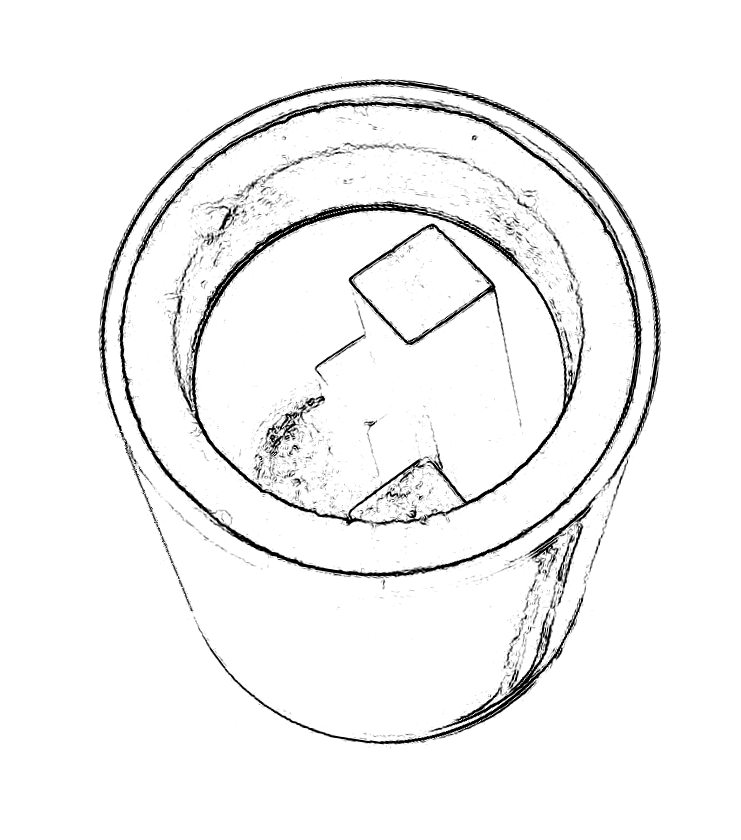
\includegraphics[width=0.8\textwidth]{Ilustrations/Calorimetro.png}
	\caption{Calorímetro aberto.}
\end{marginfigure}

Para determinar o calor específico devemos tomar o calorímetro com uma massa $m$ de água fria, ambos em equilíbrio térmico a uma temperatura inicial $T_i$. Se tomarmos uma amostra aquecida a uma temperatura $T_q$ e a adicionarmos ao calorímetro, temos após o equilíbrio uma temperatura final $T_f$. Analisando as trocas de calor obtemos
\begin{align}
    \Delta E_S^{\text{mec}} + \Delta E_S^{\text{int}} &= W_{F_{\text{ext}}} + Q + R \\
    \Delta E_S^{\text{int}} &= 0,
\end{align}
%
onde novamente temos que não ocorrem variações de energia mecânica apreciáveis e também que não temos trocas de calor, radiação, ou trabalho de forças externas entre o calorímetro e o ambiente. Como a energia interna de cada componente pode variar independentemente,
\begin{equation}
    \Delta E_{\text{água quente}}^{\text{int}} + \Delta E_{\text{água fria}}^{\text{int}} + \Delta E_{\text{calorímetro}}^{\text{int}} = 0,
\end{equation}
%
o que resulta em
\begin{equation}
	Q^{\text{Corpo}}_{\text{perdido}} + Q^{\text{água}}_{\text{ganho}} + Q^{\text{Calorímetro}}_{\text{ganho}} = 0
\end{equation}
%
Substituindo as expressões $Q = m c \Delta T$ para o ganho de calor pela água, $Q = m_a c_a \Delta T$ para o calor perdido pela amostra, e $Q = C\Delta T$ para o calor ganho pelo calorímetro, temos
\begin{equation}
	m_a c_a (T_f - T_q) + m c (T_f - T_i) + C (T_f-T_i) = 0.
\end{equation}
%
Obtemos então para o calor específico da amostra
\begin{equation}
	c_a = - \left[\frac{(mc + C)\cdot(T_f - T_i)}{m_a (T_f - T_q)}\right]
\end{equation}

%%%%%%%%%%%%%%%%%%%%%%%%%%%%%%%%%%%%%%%%%%%%%%%%%%%%%%%%%%%%%%%%%%%%%%%%%%%%%%%
\section{Experimento}
%%%%%%%%%%%%%%%%%%%%%%%%%%%%%%%%%%%%%%%%%%%%%%%%%%%%%%%%%%%%%%%%%%%%%%%%%%%%%%%

%%%%%%%%%%%%%%%%%%%%%%
\subsection{Objetivos}
\label{Sec:ObjetivosCalorEspecifico}
%%%%%%%%%%%%%%%%%%%%%%

\begin{enumerate}
	\item Determinar experimentalmente o calor específicos de diferentes materiais sólidos;
	\item Observar o equilíbrio térmico entre os corpos;
	\item Observar a validade da Primeira Lei da Termodinâmica;
\end{enumerate}

%%%%%%%%%%%%%%%%%%%%%%%%%%%%%%%%%%%%%%%%%%%%%%%%%%%%%%%%%%%%%%%%%%%%%%%%%%%%%%%
\section{Material Necessário}
%%%%%%%%%%%%%%%%%%%%%%%%%%%%%%%%%%%%%%%%%%%%%%%%%%%%%%%%%%%%%%%%%%%%%%%%%%%%%%%

\begin{itemize}
	\item Calorímetro;
	\item Termômetro de haste;
	\item Becker com água fria;
	\item Becker de vidro;
	\item Ebulidores elétricos.
	\item Termômetro;
	\item Balança;
	\item Pinça;
	\item Corpos de diferentes materiais;
	\item Recipiente para descartar água.
\end{itemize}

\begin{figure}[!hbt]
	\centering
	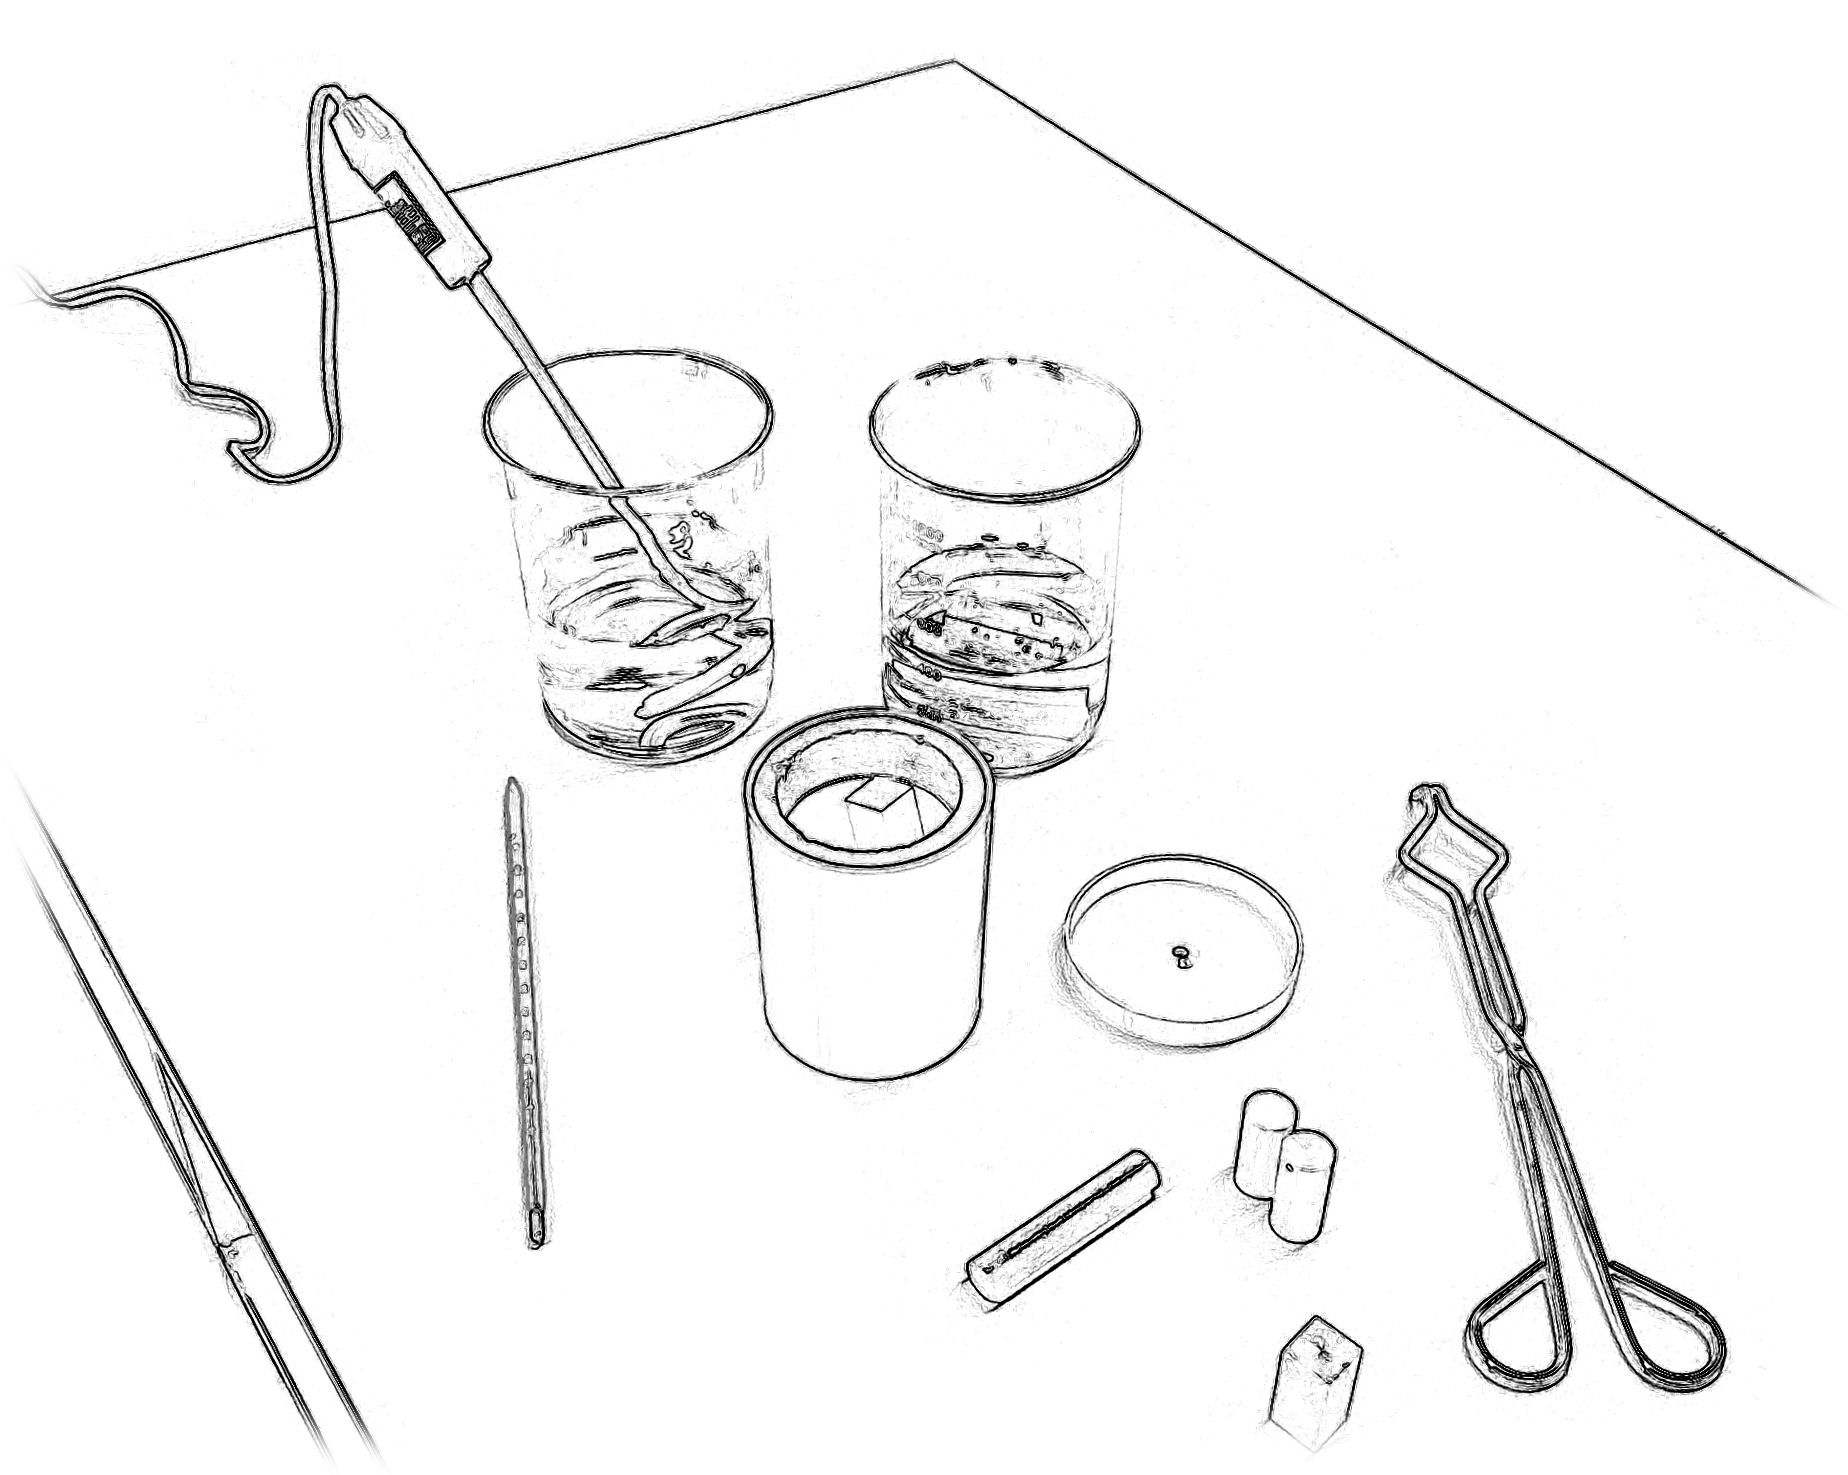
\includegraphics[width=0.7\textwidth]{Ilustrations/AparatoCalorEspecifico}
	\caption{Aparato para a verificação do calor específico de sólidos.}
\end{figure}

%%%%%%%%%%%%%%%%%%%%%%%%%%%%%%%%%%%%%%%%%%%%%%%%%%%%%%%%%%%%%%%%%%%%%%%%%%%%%%%
\section{Procedimento Experimental}
%%%%%%%%%%%%%%%%%%%%%%%%%%%%%%%%%%%%%%%%%%%%%%%%%%%%%%%%%%%%%%%%%%%%%%%%%%%%%%%

%%%%%%%%%%%%%%%%%%%%%
\subsection{Determinação da Capacidade Térmica do Calorímetro} % Se necessário
%%%%%%%%%%%%%%%%%%%%%
\begin{enumerate}
	\item Determine a massa $m^{\text{Cal}}$ do calorímetro com o auxílio da balança, anote o resultado na Tabela~\ref{Tab:CapacidadeTermica};
	\item Adicione água fria\footnote{Aqui ``água fria'' se refere a água a qualquer temperatura significativamente menor que a temperatura da água quente utilizada. Se a temperatura da água quente for de aproximadamente \np[\tcdegree C]{100,0}, por exemplo, para os nossos propósitos podemos considerar água à temperatura ambiente como fria.} ao calorímetro até que ela cubra aproximadamente um quarto da parte metálica interna;
	\item Verifique a massa $m^{\text{Cal}}_{\text{água fria}}$ do calorímetro com a água e anote na Tabela~\ref{Tab:CapacidadeTermica};
	\item Aguarde até que o sistema entre em equilíbrio térmico. Uma vez atingido o equilíbrio, com o auxílio do termômetro, determine a temperatura inicial $T_i$ do calorímetro e a anote na Tabela~\ref{Tab:CapacidadeTermica}. A partir de agora, mantenha o calorímetro sempre tampado;
	\item Verifique a temperatura da água quente disponível e anote na Tabela~\ref{Tab:CapacidadeTermica};
	\item Imediatamente após verificar a temperatura da água quente, adicione água quente ao calorímetro até cobrir aproximadamente a metade da cuba metálica interna. Aguarde o equilíbrio e verifique a temperatura final $T_f$ do calorímetro, anotando na Tabela~\ref{Tab:CapacidadeTermica};
	\item Verifique a massa final $m^{\text{Cal}}_{\text{água fria+quente}}$ do sistema;
	\item Descarte a água do calorímetro e repita o procedimento descrito acima mais duas vezes, anotando os dados na Tabela~\ref{Tab:CapacidadeTermica}
\end{enumerate}

%%%%%%%%%%%%%%%%%%%%%%%%%%%%%%%%%%%%%%%%%%%%%%%%%%%%%%%%
\subsection{Determinação do calor específico de sólidos}
%%%%%%%%%%%%%%%%%%%%%%%%%%%%%%%%%%%%%%%%%%%%%%%%%%%%%%%%

\begin{enumerate}
	\item Determine a massa $m^{\text{Cal}}$ do calorímetro com o auxílio da balança, anote o resultado na Tabela~\ref{Tab:CalorEspecificoCorpo1};
	\item Adicione água fria ao calorímetro até que ela cubra aproximadamente um quarto da parte metálica interna;
	\item Verifique a massa $m^{\text{Cal}}_{\text{água fria}}$ do calorímetro com a água fria e anote na Tabela~\ref{Tab:CalorEspecificoCorpo1};
	\item Aguarde até que o sistema entre em equilíbrio térmico. Uma vez atingido o equilíbrio, com o auxílio do termômetro, determine a temperatura inicial $T_i$ do calorímetro e a anote na Tabela~\ref{Tab:CalorEspecificoCorpo1}. A partir de agora, mantenha o calorímetro sempre tampado;
	\item Tome um dos materiais\footnote{Se houver mais que uma amostra do mesmo material disponível, tome mais que uma. Quanto maior for a massa, menor será o erro na determinação do calor específico.} e o submerja na água quente. Aguarde até que a amostra entre em equilíbrio térmico com a água. Verifique a temperatura $T_{\text{amostra}}$ do banho térmico e anote na Tabela~\ref{Tab:CalorEspecificoCorpo1}.
	\item Retire a amostra do banho quente e a coloque rapidamente no calorímetro. Aguarde o equilíbrio térmico\footnote{Se as amostras forem metálicas, o equilíbrio será atingido rapidamente. Não aguarde um tempo muito longo pois nesse caso a energia térmica perdida pelo calorímetro para o ambiente será significativa.} e verifique temperatura final $T_f$ do calorímetro. Anote os resultados na Tabela~\ref{Tab:CalorEspecificoCorpo1}.
	\item Retire a amostra do calorímetro, seque-a e verifique sua massa\footnote{Caso a amostra do material seja um corpo rígido, não é necessário aferir sua massa novamente.} $m_{\text{a}}$ com o auxílio da balança e a anote na Tabela~\ref{Tab:CalorEspecificoCorpo1}.
	\item Repita o procedimento acima mais duas vezes para o mesmo material. Após finalizar os procedimentos para o material em questão, repita o procedimento para outros dois materiais (três vezes cada), anotando os resultados nas Tabelas~\ref{Tab:CalorEspecificoCorpo2} a~\ref{Tab:CalorEspecificoCorpo3}.
\end{enumerate}

%%%%%%%%%%%%%%%%%%%%%%%%%%%%%%%%%%%%%%%%%%%%%%%%%%%%%%%%%%%%%%%%%%%%%%%%%%%%%%%
%%%%%%%%%%%%%%%%%%%%%%%%%%%%%%%%%%%%%%%%%%%%%%%%%%%%%%%%%%%%%%%%%%%%%%%%%%%%%%%
%%%%%%%%%%%%%%%%%%%%%%%%%%%%%%%%%%%%%%%%%%%%%%%%%%%%%%%%%%%%%%%%%%%%%%%%%%%%%%%
%%%%%%%%%%%%%%%%%%%%%%%%%%%%%%%%%%%%%%%%%%%%%%%%%%%%%%%%%%%%%%%%%%%%%%%%%%%%%%%
\cleardoublepage

\noindent{}{\huge\textit{Calor Específico de Sólidos}}

\vspace{15mm}

\begin{fullwidth}
\noindent{}\makebox[0.6\linewidth]{Turma:\enspace\hrulefill}\makebox[0.4\textwidth]{  Data:\enspace\hrulefill}
\vspace{5mm}

\noindent{}\makebox[0.6\linewidth]{Aluno(a):\enspace\hrulefill}\makebox[0.4\textwidth]{  Matrícula:\enspace\hrulefill}

\noindent{}\makebox[0.6\linewidth]{Aluno(a):\enspace\hrulefill}\makebox[0.4\textwidth]{  Matrícula:\enspace\hrulefill}

\noindent{}\makebox[0.6\linewidth]{Aluno(a):\enspace\hrulefill}\makebox[0.4\textwidth]{  Matrícula:\enspace\hrulefill}

\noindent{}\makebox[0.6\linewidth]{Aluno(a):\enspace\hrulefill}\makebox[0.4\textwidth]{  Matrícula:\enspace\hrulefill}

\noindent{}\makebox[0.6\linewidth]{Aluno(a):\enspace\hrulefill}\makebox[0.4\textwidth]{  Matrícula:\enspace\hrulefill}
\end{fullwidth}

\vspace{5mm}

%%%%%%%%%%%%%%%%%%%%%%%%%%%%%%%%%%%%%%%%%%%%%%%%%%%%%%%%%%%%%%%%%%%%%%%%%%%%%%%
\section{Questionário}
%%%%%%%%%%%%%%%%%%%%%%%%%%%%%%%%%%%%%%%%%%%%%%%%%%%%%%%%%%%%%%%%%%%%%%%%%%%%%%%

\begin{question}[type={exam}]{1}
Apresente os resultados de maneira clara e organizada. Mostre os cálculos requisitados de maneira clara e sucinta, evidenciando o raciocínio desenvolvido.
\end{question}

\begin{question}[type={exam}]{1}
Liste os equipamentos utilizados. Para os instrumentos de medida, descreva o tipo do equipamento, sua resolução, e seu erro de escala.
\end{question}

\begin{question}[type={exam}]{1.5}
Preencha as tabelas com o número adequado de algarismos significativos, unidades, e erros de escala apropriados. 
\end{question}

\begin{question}[type={exam}]{2}
Calcule a capacidade térmica do calorímetro, juntamente com o erro propagado, para as três medidas realizadas. Obtenha o valor médio e o erro associado.
\end{question}

\begin{question}[type={exam}]{2}
Utilizando o resultado para a capacidade térmica do calorímetro e o erro associado a ela, calcule os calores específicos dos materiais, incluindo o erro propagado, para cada uma das três medidas de cada material. Obtenha o valor médio e o erro associado para cada material.
\end{question}

\begin{question}[type={exam}]{1}
Identifique o material e compare o resultado obtido para o calor específico com os valores de referência na Tabela~\ref{Tab:CaloresEspecificosDeReferencia}. Calcule os erros percentuais utilizando
\begin{equation}
	E_{\%} = \left|\frac{x-x_{\text{ref}}}{x_{\text{ref}}}\right| \times 100.
\end{equation}
\end{question}

\begin{question}[type={exam}]{1.5}
Considerando os objetivos do experimento, listados na Seção~\ref{Sec:ObjetivosCalorEspecifico}, e os resultados obtidos nas questões anteriores, discuta quais objetivos foram atingidos com sucesso, justificando suas conclusões. Se algum objetivo não foi atingido, discuta quais são os possíveis motivos do fracasso e que providências podem ser tomadas para que eles sejam alcançados.
\end{question}

\vfill
%%%%%%%%%%%%%%%%%%%%%%%%%%%%%%%%%%%%%%%%%%%%%%%%%%%%%%%%%%%%%%%%%%%%%%%%%%%%%%%
\pagebreak
\section{Tabelas}
%%%%%%%%%%%%%%%%%%%%%%%%%%%%%%%%%%%%%%%%%%%%%%%%%%%%%%%%%%%%%%%%%%%%%%%%%%%%%%%

\begin{table*}[!ht]
\centering
	\begin{tabular}{lp{22mm}p{22mm}p{22mm}lp{22mm}p{22mm}l}
		\toprule
		&\multicolumn{5}{l}{\textbf{Determinação da Capacidade Térmica do calorímetro}}\\
		\\
		\cmidrule{2-7}
		& Massas & \\
		\cmidrule{2-7}
		& $m^{\text{Cal}}$ & $m^{\text{Cal}}_{\text{água fria}}$ & $m^{\text{Cal}}_{\text{água fria+quente}}$ & & $m_{\text{fria}}^{\text{água}}$ & $m_{\text{quente}}^{\text{água}}$ & \\
		\cmidrule{2-4}\cmidrule{6-7}
		& \cellcolor[gray]{0.95} & \cellcolor[gray]{0.97} & \cellcolor[gray]{0.95} & & \cellcolor[gray]{0.95} & \cellcolor[gray]{0.97} & \\
		& \cellcolor[gray]{0.89} & \cellcolor[gray]{0.92} & \cellcolor[gray]{0.89} & & \cellcolor[gray]{0.89} & \cellcolor[gray]{0.92} & \\
		& \cellcolor[gray]{0.95} & \cellcolor[gray]{0.97} & \cellcolor[gray]{0.95} & & \cellcolor[gray]{0.95} & \cellcolor[gray]{0.97} & \\
		\cmidrule{2-7}
		\\
		& Temperaturas \\
		\cmidrule{2-7}
		& $T_{i}$ & $T^{\text{água}}_{\text{quente}}$ & $T_{f}$ & & $T_f - T_i$ & $T_f - T^{\text{água}}_{\text{quente}}$ \\
		\cmidrule{2-4} \cmidrule{6-7}
		& \cellcolor[gray]{0.95} & \cellcolor[gray]{0.97} & \cellcolor[gray]{0.95} & & \cellcolor[gray]{0.95} & \cellcolor[gray]{0.97} & \\
		& \cellcolor[gray]{0.89} & \cellcolor[gray]{0.92} & \cellcolor[gray]{0.89} & & \cellcolor[gray]{0.89} & \cellcolor[gray]{0.92} & \\
        & \cellcolor[gray]{0.95} & \cellcolor[gray]{0.97} & \cellcolor[gray]{0.95} & & \cellcolor[gray]{0.95} & \cellcolor[gray]{0.97} & \\
		\cmidrule{2-7}
		\bottomrule
	\end{tabular}
	\caption[][0.5cm]{Dados para o cálculo da capacidade térmica do calorímetro.}
	\label{Tab:CapacidadeTermica}
\end{table*}
\vspace{2cm}
\begin{table*}[!ht]\forceversofloat
\centering
	\begin{tabular}{lp{22mm}p{22mm}p{22mm}lp{22mm}p{22mm}l}
		\toprule
        \multicolumn{6}{l}{\textbf{Determinação do Calor Específico, Material N\textordmasculine~1}}\\
        \\
		& Massas \\
		\cmidrule{2-6}
		& $m^{\text{Cal}}$ & $m^{\text{Cal}}_{\text{água fria}}$ & $m_{\text{a}}$ & & $m_{\text{fria}}^{\text{água}}$ & \\
		\cmidrule{2-4} \cmidrule{6-6}
		& \cellcolor[gray]{0.95} & \cellcolor[gray]{0.97} & \cellcolor[gray]{0.95} & & \cellcolor[gray]{0.95} & \\
		& \cellcolor[gray]{0.89} & \cellcolor[gray]{0.92} & \cellcolor[gray]{0.89} & & \cellcolor[gray]{0.89} & \\
		& \cellcolor[gray]{0.95} & \cellcolor[gray]{0.97} & \cellcolor[gray]{0.95} & & \cellcolor[gray]{0.95} & \\
		\cmidrule{2-6}
		\\
		& Temperaturas \\
		\cmidrule{2-4}\cmidrule{6-7}
		& $T_{i}$ & $T_{\text{amostra}}$ & $T_{f}$ & & $T_f - T_i$ & $T_f - T_{\text{amostra}}$ & \\
		\cmidrule{2-4}\cmidrule{6-7}
		& \cellcolor[gray]{0.95} & \cellcolor[gray]{0.97} & \cellcolor[gray]{0.95} & & \cellcolor[gray]{0.95} & \cellcolor[gray]{0.97} & \\
		& \cellcolor[gray]{0.89} & \cellcolor[gray]{0.92} & \cellcolor[gray]{0.89} & & \cellcolor[gray]{0.89} & \cellcolor[gray]{0.92} & \\
		& \cellcolor[gray]{0.95} & \cellcolor[gray]{0.97} & \cellcolor[gray]{0.95} & & \cellcolor[gray]{0.95} & \cellcolor[gray]{0.97} & \\
		\cmidrule{2-7}
		\bottomrule
	\end{tabular}
	\caption[][0.5cm]{Dados para o cálculo do calor específico.}
	\label{Tab:CalorEspecificoCorpo1}
\end{table*}
\vfill
\pagebreak

\begin{table*}[!ht]\forcerectofloat
\centering
	\begin{tabular}{lp{22mm}p{22mm}p{22mm}lp{22mm}p{22mm}l}
		\toprule
        \multicolumn{6}{l}{\textbf{Determinação do Calor Específico, Material N\textordmasculine~2}}\\
        \\
		& Massas \\
		\cmidrule{2-6}
		& $m^{\text{Cal}}$ & $m^{\text{Cal}}_{\text{água fria}}$ & $m_{\text{a}}$ & & $m_{\text{fria}}^{\text{água}}$ & \\
		\cmidrule{2-4} \cmidrule{6-6}
		& \cellcolor[gray]{0.95} & \cellcolor[gray]{0.97} & \cellcolor[gray]{0.95} & & \cellcolor[gray]{0.95} & \\
		& \cellcolor[gray]{0.89} & \cellcolor[gray]{0.92} & \cellcolor[gray]{0.89} & & \cellcolor[gray]{0.89} & \\
		& \cellcolor[gray]{0.95} & \cellcolor[gray]{0.97} & \cellcolor[gray]{0.95} & & \cellcolor[gray]{0.95} & \\
		\cmidrule{2-6}
		\\
		& Temperaturas \\
		\cmidrule{2-4}\cmidrule{6-7}
		& $T_{i}$ & $T_{\text{amostra}}$ & $T_{f}$ & & $T_f - T_i$ & $T_f - T_{\text{amostra}}$ & \\
		\cmidrule{2-4}\cmidrule{6-7}
		& \cellcolor[gray]{0.95} & \cellcolor[gray]{0.97} & \cellcolor[gray]{0.95} & & \cellcolor[gray]{0.95} & \cellcolor[gray]{0.97} & \\
		& \cellcolor[gray]{0.89} & \cellcolor[gray]{0.92} & \cellcolor[gray]{0.89} & & \cellcolor[gray]{0.89} & \cellcolor[gray]{0.92} & \\
		& \cellcolor[gray]{0.95} & \cellcolor[gray]{0.97} & \cellcolor[gray]{0.95} & & \cellcolor[gray]{0.95} & \cellcolor[gray]{0.97} & \\
		\cmidrule{2-7}
		\bottomrule
	\end{tabular}
	\caption[][0.5cm]{Dados para o cálculo do calor específico.}
	\label{Tab:CalorEspecificoCorpo2}
\end{table*}
\vspace{2cm}
\begin{table*}[!ht]\forcerectofloat
\centering
	\begin{tabular}{lp{22mm}p{22mm}p{22mm}lp{22mm}p{22mm}l}
		\toprule
        \multicolumn{6}{l}{\textbf{Determinação do Calor Específico, Material N\textordmasculine~3}}\\
        \\
		& Massas \\
		\cmidrule{2-6}
		& $m^{\text{Cal}}$ & $m^{\text{Cal}}_{\text{água fria}}$ & $m_{\text{a}}$ & & $m_{\text{fria}}^{\text{água}}$ & \\
		\cmidrule{2-4} \cmidrule{6-6}
		& \cellcolor[gray]{0.95} & \cellcolor[gray]{0.97} & \cellcolor[gray]{0.95} & & \cellcolor[gray]{0.95} & \\
		& \cellcolor[gray]{0.89} & \cellcolor[gray]{0.92} & \cellcolor[gray]{0.89} & & \cellcolor[gray]{0.89} & \\
		& \cellcolor[gray]{0.95} & \cellcolor[gray]{0.97} & \cellcolor[gray]{0.95} & & \cellcolor[gray]{0.95} & \\
		\cmidrule{2-6}
		\\
		& Temperaturas \\
		\cmidrule{2-4}\cmidrule{6-7}
		& $T_{i}$ & $T_{\text{amostra}}$ & $T_{f}$ & & $T_f - T_i$ & $T_f - T_{\text{amostra}}$ & \\
		\cmidrule{2-4}\cmidrule{6-7}
		& \cellcolor[gray]{0.95} & \cellcolor[gray]{0.97} & \cellcolor[gray]{0.95} & & \cellcolor[gray]{0.95} & \cellcolor[gray]{0.97} & \\
		& \cellcolor[gray]{0.89} & \cellcolor[gray]{0.92} & \cellcolor[gray]{0.89} & & \cellcolor[gray]{0.89} & \cellcolor[gray]{0.92} & \\
		& \cellcolor[gray]{0.95} & \cellcolor[gray]{0.97} & \cellcolor[gray]{0.95} & & \cellcolor[gray]{0.95} & \cellcolor[gray]{0.97} & \\
		\cmidrule{2-7}
		\bottomrule
	\end{tabular}
	\caption[][0.5cm]{Dados para o cálculo do calor específico.}
	\label{Tab:CalorEspecificoCorpo3}
\end{table*}
\vfill



%%%%%%%%%%%%%%%%%%%%%%%%%%%%%%%%%%%%%%%%%%%%%%%%%%%%%%%%%%%%%%%%%%%%%%%%%%%%%%%
\chapter{Zero absoluto}
\label{Chap:ExpZeroAbsoluto}
%%%%%%%%%%%%%%%%%%%%%%%%%%%%%%%%%%%%%%%%%%%%%%%%%%%%%%%%%%%%%%%%%%%%%%%%%%%%%%%

\begin{fullwidth}\it
	Realizaremos um experimento em que verificaremos a pressão exercida por uma quantidade de gás com volume constante em função de sua temperatura. Através desses dados, determinaremos a temperatura para a qual teríamos uma pressão nula --- tal temperatura é o que denominamos como Zero Absoluto ---. Utilizaremos os seguintes conceitos/técnicas de análise de dados: medidas, algarismos significativos, gráficos, software para elaboração de gráficos, erros de escala e propagados, equação geral para o erro propagado, regressão linear, linearização, erros dos coeficientes $A$ e $B$, e planilhas para cálculo dos coeficientes $A$ e $B$ com erros.
\end{fullwidth}

%%%%%%%%%%%%%%%%%%%%%%%%%%%%%%%%%%%%%%%%%%%%%%%%%%%%%%%%%%%%%%%%%%%%%%%%%%%%%%%
\section{Termômetros}
%%%%%%%%%%%%%%%%%%%%%%%%%%%%%%%%%%%%%%%%%%%%%%%%%%%%%%%%%%%%%%%%%%%%%%%%%%%%%%%

Um método simples para verificar a temperatura é utilizar alguma propriedade de um material que varie com a temperatura como indicador de leitura. Muitos termômetros empregados rotineiramente em laboratórios usam mercúrio, outros usam álcool. Em ambos os casos, a propriedade que varia com a temperatura é o volume: o líquido de um reservatório se dilata e invade um tubo fino, onde a altura da coluna pode ser lida através de uma escala.

Outras propriedades podem ser utilizadas para verificar a temperatura, dentre elas a diferença de potencial elétrico entre uma junção bimetálica, a resistência elétrica de um material, o comprimento de uma fita metálica longa, a pressão de um volume confinado de um gás, etc. 

Em todos esses casos, é necessário se utilizar dois pontos para calibrar o termômetro com valores arbitrários de temperatura. A escala Celsius, por exemplo, utiliza a temperatura de fusão do gelo para zero graus e a temperatura de ebulição da água para 100 graus. No caso de um termômetro de mercúrio, podemos verificar a altura da coluna para a temperatura de fusão do gelo, realizando uma marca (na escala Celsius, \np[\tcdegree]{0}). Marcamos também a altura da coluna para a temperatura de ebulição da água (\np[\tcdegree]{100}). Dividimos então o intervalo entre essas duas marcas em um número de divisões menores. Podemos então verificar qualquer temperatura intermediária utilizando uma leitura da coluna de mercúrio. Podemos inclusive extrapolar as leituras para valores de temperatura maiores e menores que os extremos definidos pela temperatura de fusão do gelo e de ebulição da água, bastando para isso manter o tamanho da divisão igual às divisões intermediárias.

A confiabilidade das medidas de temperatura obtidas através de um termômetro está diretamente ligada à linearidade da propriedade observada com a variação da temperatura. Para faixas de temperatura relativamente pequenas, isso pode não ser um problema, mas se desejarmos realizar medições para uma ampla faixa de valores, comportamentos não-lineares podem ter efeito significativo. Além disso, se --- por exemplo --- desejarmos utilizar uma medida de temperatura extremamente elevada, não podemos utilizar um termômetro devido ao risco de danificá-lo\footnote{Nesse caso, podemos verificar a temperatura através do espectro da radiação emitida pelo corpo em questão.}. Portanto, é importante escolher um material e uma propriedade adequados à medida em questão.

%%%%%%%%%%%%%%%%%%%%%%%%%%%%%%%%%%%%%%%%%%%%%%%%%%
\subsection{Termômetros de gás a volume constante}
%%%%%%%%%%%%%%%%%%%%%%%%%%%%%%%%%%%%%%%%%%%%%%%%%%

Uma propriedade que pode ser utilizada para realizar uma medida confiável da temperatura é a pressão de um gás mantido em um volume constante. Segundo a equação dos gases ideais, a pressão varia com a temperatura de acordo com\footnote[][-1cm]{As temperaturas devem estar na escala Kelvin, discutida adiante.}
\begin{equation}
	PV = nRT,
\end{equation}
%
onde $R$ é a constante dos gases, $n$ é o número de moles de partículas do gás, $V$ é o volume ocupado pelo gás, e $T$ é a temperatura. Dessa equação, podemos escrever
\begin{equation}\label{Eq:PvsT}
	P = \frac{nR}{V} T.
\end{equation}

\begin{marginfigure}
\centering
\begin{tikzpicture}[>=Stealth]
    \draw[->] (0,0) -- (4,0) node[below left]{$T~(\tcdegree\rm{C})$};
    \draw[->] (0,0) -- (0,3) node[below left]{$P~(\rm{Pa})$};
    
    \draw[smooth,samples=10,domain=0:3.5]
    plot(\x,{tan(7)*\x + 3*tan(7)});
     \draw[dashed, smooth,samples=10,domain=0:3.5]
    plot(\x,{tan(14)*\x + 3*tan(14)});
     \draw[dashdotted, smooth,samples=10,domain=0:3.5]
    plot(\x,{tan(20)*\x + 3*tan(20)});
   
\end{tikzpicture}
\caption{Para um gás real, a relação entre $P$ e $T$ depende do gás, porém é sempre linear.\label{Fig:RelPressaoTempGasIdeal}}
\end{marginfigure}

Para um gás real, a relação entre a pressão e a temperatura depende do tipo de gás utilizado. Porém, se o gás estiver a baixa pressão, ou seja, estiver \emph{rarefeito}, e a temperatura a ser medida for maior que aquela em que o gás se torna um líquido, podemos utilizar qualquer gás para realizar medidas de temperatura. A diferença entre diversos gases será a inclinação da reta, porém as relações serão sempre lineares (Figura~\ref{Fig:RelPressaoTempGasIdeal}).

Para um gás mantido a um volume $V$ constante em um reservatório hermético, podemos afirmar que o número de moles $n$ se mantém constante. Temos então uma relação de proporcionalidade entre a pressão do gás e a temperatura a que ele se encontra. Um dispositivo que utiliza essa propriedade para realizar medidas é denominado \emph{termômetro de gás a volume constante}.

\begin{marginfigure}
\centering
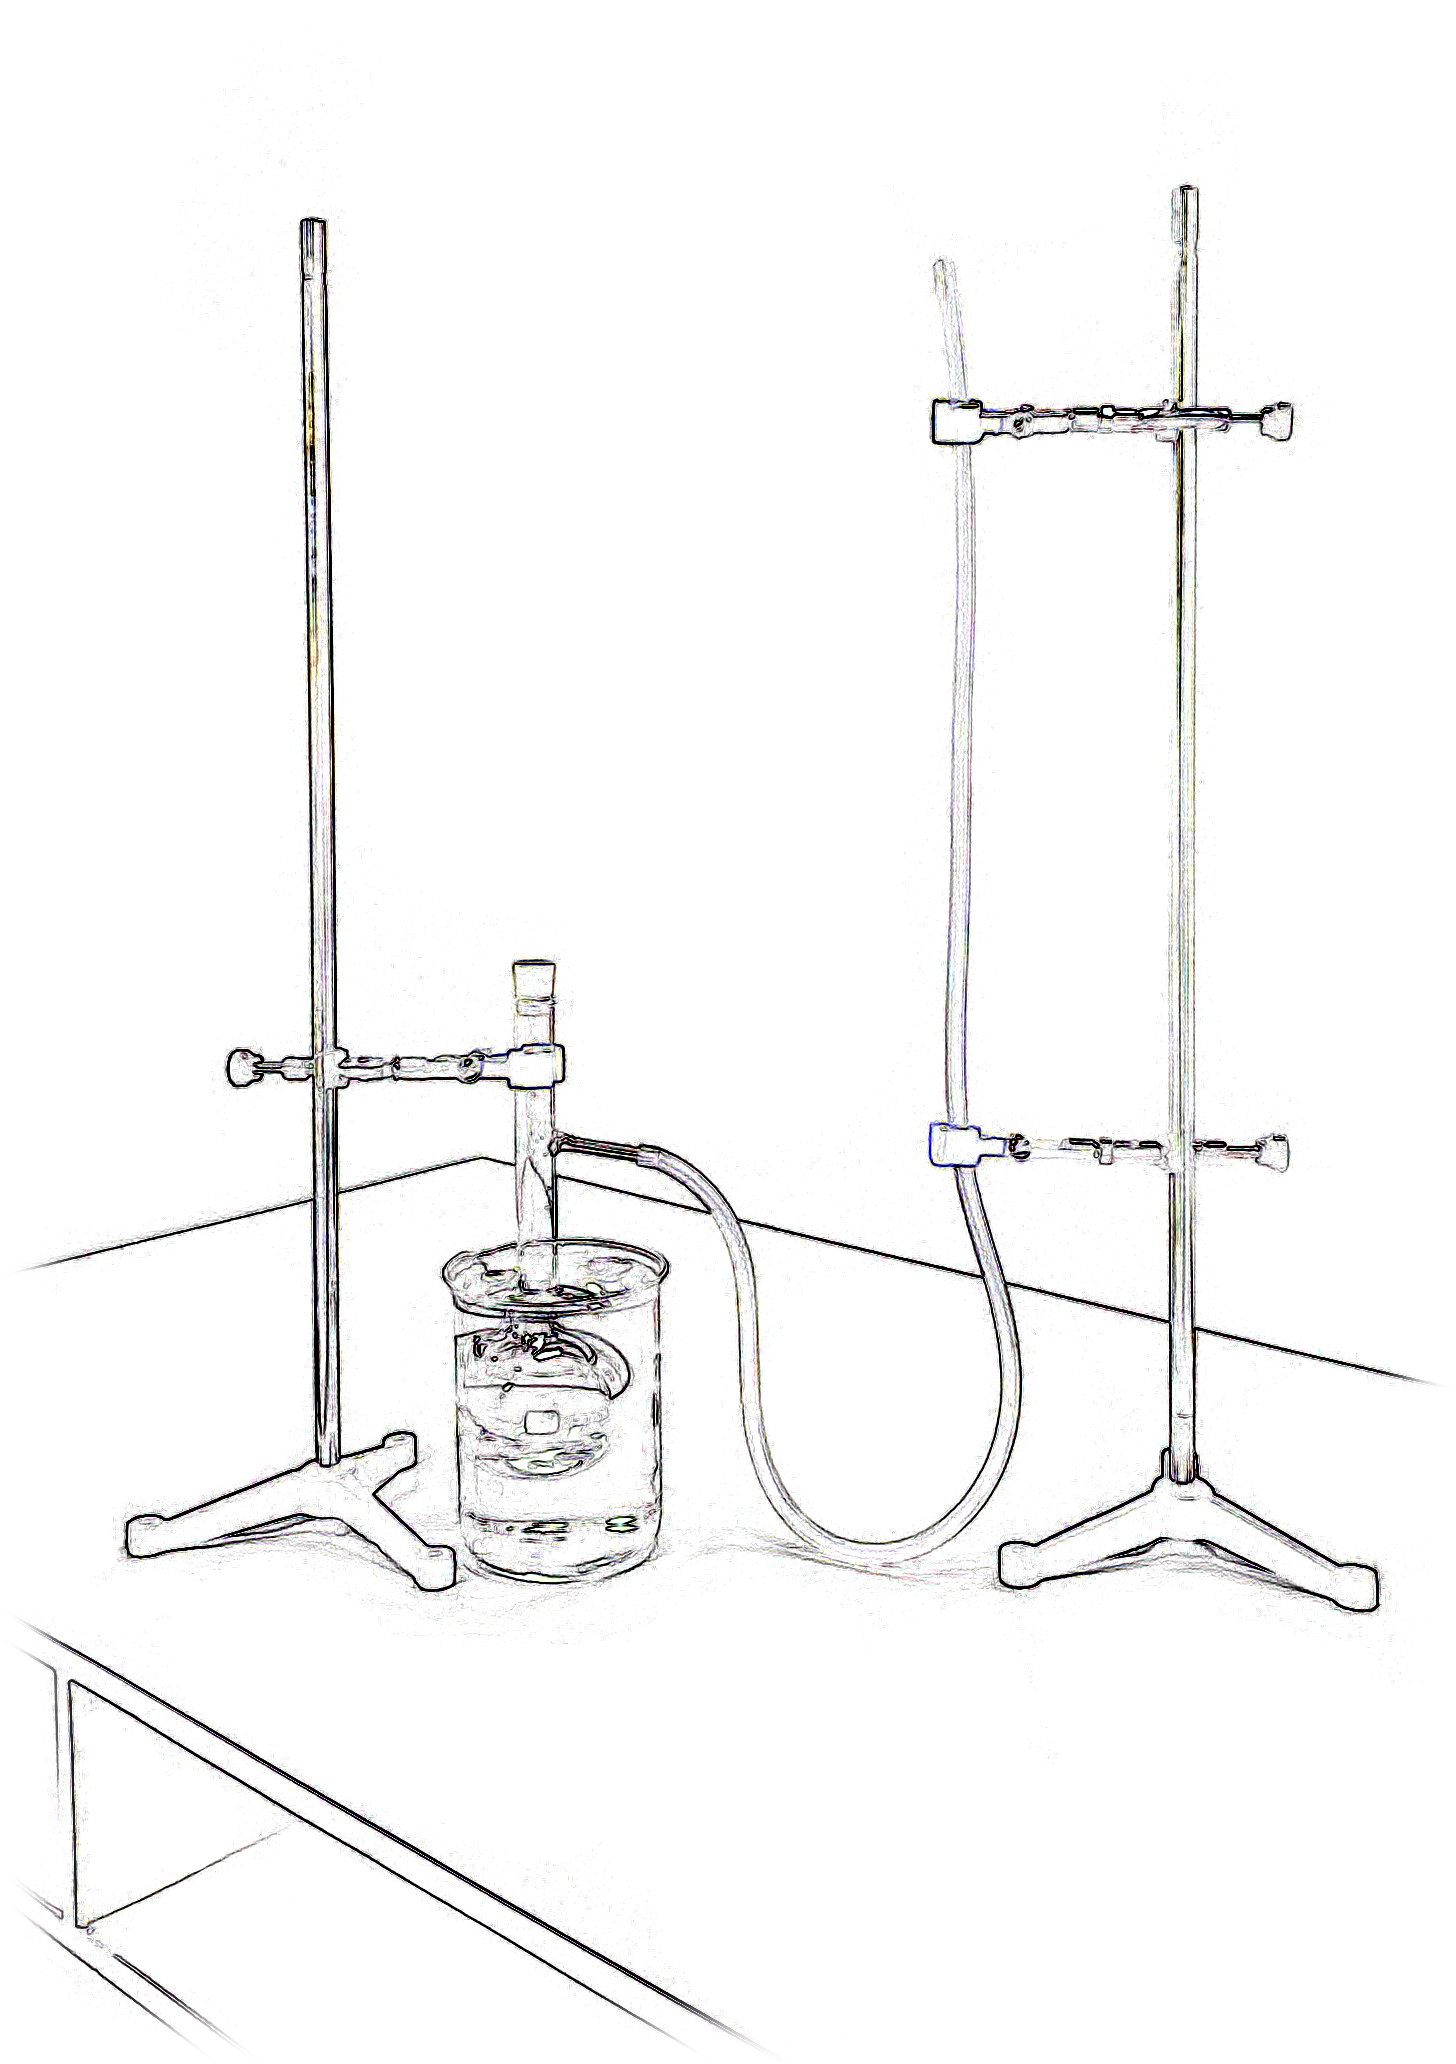
\includegraphics[width=\textwidth]{Ilustrations/Term_gas.png}
\caption{Termômetro de gás a volume constante.\label{Fig:TermometroGas}}
\end{marginfigure}

A Figura~\ref{Fig:TermometroGas} mostra um desenho esquemático de um dispositivo desse tipo: nela temos um balão de destilação fechado com uma rolha e em cuja saída lateral está conectada um tubo flexível, sendo que a outra extremidade é aberta. Dentro do tubo temos um fluido de densidade conhecida. O balão fica submerso em um banho térmico cuja temperatura estamos interessados em medir.

Como a extremidade livre do tubo é aberta, ela está sujeita à pressão atmosférica, logo, a pressão do gás dentro do balão será determinada pela soma da pressão atmosférica com a pressão exercida pela coluna de líquido:
\begin{equation}\label{Eq:PressaoColunaFluido}
	P = P_0 + \rho g h,
\end{equation}
%
onde $P_0$ é a pressão atmosférica, $\rho$ é a densidade do fluido dentro do tubo, $g$ é a aceleração da gravidade e $h$ é a altura\footnote{Note que $h$ é a \emph{altura} da coluna, não seu comprimento. Tal distância deve ser medida \emph{verticalmente}.} (veja a Figura~\ref{Fig:FigEsquematicaTermGas}).

Para determinarmos o valor da altura da coluna de fluido adequadamente, devemos nos certificar que o volume de gás dentro do balão seja mantido constante. Para isso, devemos verificar a posição da coluna de fluido na extremidade do tubo que está ligada ao balão e marcarmos sua posição para referência futura (tal marca é representada pela seta na Figura~\ref{Fig:FigEsquematicaTermGas}). Ao aquecermos o gás, o fluido no tubo se deslocará devido à pressão exercida sobre ele, fazendo com que as posições dos topos das colunas em ambas as extremidades do tubo  mudem de posição. Para que o gás volte ao volume inicial, o topo da coluna da extremidade do tubo ligada ao balão deve voltar ao nível original, o que pode ser feito deslocando a extremidade livre para cima. Só então devemos aferir a distância vertical $h$ entre as colunas.

\begin{marginfigure}[-4cm]
\centering
\begin{tikzpicture}[>=Stealth,
interface/.style={
        % superfície
        postaction={draw,decorate,decoration={border,angle=-45,
                    amplitude=0.2cm,segment length=2mm}}}
    ]
    
    \draw[pattern = north west lines] (-1,1.5) -- (-1, 0) -- (1,0) -- (1,1.5) -- (0.9,1.5) -- (0.9,0.1) -- (-0.9,0.1) -- (-0.9, 1.5) -- cycle;
    
    % balão
    \draw (0,0.75)+(95:0.5) arc[radius = 0.5, start angle = -265, end angle = 85];
    \draw (0,0.75)++(95:0.5) -- +(0,1) coordinate (be);
    \draw (0,0.75)++(85:0.5) -- +(0,0.5) coordinate (li);
    \draw (li) ++(0,0.05) coordinate (ls) -- +(0,0.45) coordinate (bd);
    \draw (li) -- +(-5:0.3) coordinate (si);
    \draw (ls) -- +(-5:0.3);
    \draw[fill] (0,2.25)+(-0.05,0) rectangle +(0.05,0.1);
    \node (P) at (0,0.75) {$P$};
    
    % mangueira
    \draw[double = white, double distance = 0.05cm] (si)+(0,0.025) .. controls (1,1.65) and (1.5,2) .. (1.5,1);
    
    % tubo em U
    \draw (1.475, 1) -- (1.475, 0.25) arc[start angle = -180, end angle = 0, radius = 0.2] -- +(0,2);
    \draw (1.525, 1) -- (1.525, 0.25) arc[start angle = -180, end angle = 0, radius = 0.15] -- +(0,2);
    \draw[fill] (1.475, 0.75) -- (1.475, 0.25) arc[start angle = -180, end angle = 0, radius = 0.2] -- ++(0,1) -- ++(-0.05,0) -- ++(0,-1) arc[start angle = 0, end angle = -180, radius = 0.15] -- ++(0,0.5) -- cycle;  
    
    % marca de referência
    \draw[->] (1.2, 0.75) -- (1.455,0.75);
    
    % altura da coluna
    \draw[dotted] (1.455,0.75) -- (2.2,0.75);
    \draw[dotted] (1.875,1.25) -- (2.2,1.25);
    \draw[->] (2.2, 0.25) -- (2.2, 2.25) node[below right]{$y$};
    \draw[|-|] (2.2,0.75) node[right]{$0$} -- (2.2,1.25) node[right]{$y = h$};
    
    % líquido
    \draw[pattern = dots] (0,0.75)+(95:0.5) arc[radius = 0.5, start angle = -265, end angle = 85] -- ++(0,0.15) -- (0.9, 1.4) -- (0.9,0.1) -- (-0.9,0.1) -- (-0.9,1.4) -- (-0.044,1.4) -- cycle;
    
    % mesa
    \draw[interface] (-1.25,0) -- (3.25,0);
    
\end{tikzpicture}
\caption{A pressão do gás pode ser determinada pela soma da pressão atmosférica com a pressão exercida pela coluna d'água cuja altura é $h$. O gás deve ser mantido a volume constante, o que implica que a coluna d'água na extremidade do tubo ligado ao balão deve ser mantida na marca de referência indicada pela flecha.\label{Fig:FigEsquematicaTermGas}}
\end{marginfigure}

\begin{marginfigure}[2cm]
\centering
\begin{tikzpicture}[>=Stealth]
    \draw[->] (0,0) -- (4,0) node[below left]{$h$};
    \draw[->] (0,0) -- (0,3.5) node[below left]{$T$};
    
    \draw (0,1) -- (3.5,3);
    \draw[dotted] (0.75,0) node[below]{$h_f$} -- (0.75, 1.43) -- (0, 1.43) node[left]{$T_f$};
    \draw[dotted] (3,0) node[below]{$h_e$} -- (3, 2.71) -- (0, 2.71) node[left]{$T_e$};
   
\end{tikzpicture}
\caption{A relação entre a temperatura $T$ e a altura $h$ é linear, o que nos permite utilizá-la como a escala de um termômetro.}
\end{marginfigure}

Como sabemos que existe uma relação linear da temperatura com a pressão, e uma relação linear da pressão com a altura $h$ da coluna, podemos determinar uma relação linear entre a temperatura $T$ e a altura $h$: de acordo com a Equação~\eqref{Eq:PvsT}, podemos escrever
\begin{equation}
    T = \frac{V}{nR} P,
\end{equation}
%
ou, usando a Equação~\eqref{Eq:PressaoColunaFluido},
\begin{align}
    T &= \frac{V}{nR} (P_0 + \rho g h) \\
    &= \frac{VP_0}{nR} + \frac{V\rho g}{nR}h.
\end{align}

Para que possamos definir valores numéricos específicos de temperatura, precisamos de duas temperaturas de referência, como as de fusão e ebulição da água, por exemplo. Uma vez determinados os valores arbitrários de temperatura $T_f$ e $T_e$ e as alturas $h_f$ e $h_e$ correspondentes a tais temperaturas, podemos determinar a relação entre $T$ e $h$ considerando que a tal relação é linear, o que implica em uma forma dada por
\begin{equation}
    T = Bh + A,
\end{equation}
%
onde
\begin{equation}
\begin{system} B h_e + A &= T_e \\ B h_f + A &= T_f. \end{system}
\end{equation}
%
Resolvendo esse sistema, obtemos
\begin{align}
    B &= \frac{T_e - T_f}{h_e - h_f} \\
    A &= T_f - \frac{T_e - T_f}{h_e - h_f} h_f,
\end{align}
%
de onde obtemos
\begin{equation}
    T = (h - h_f)\frac{T_e - T_f}{h_e - h_f} + T_f.
\end{equation}
 
%%%%%%%%%%%%%%%%%%%%%%%%%%
\subsection{Zero absoluto}
%%%%%%%%%%%%%%%%%%%%%%%%%%

Para qualquer gás utilizado no termômetro, a medida que a temperatura diminui, a pressão do gás também diminui. Essa relação deve ter um valor para o qual a pressão exercida pelo gás é nula, correspondendo a uma temperatura mínima ou um \emph{zero absoluto} para a escala de temperatura. Apesar de a inclinação das retas de $P \times T$ serem diferentes para gases diferentes, o valor para o qual a pressão é zero é o mesmo para qualquer gás, sendo que tal valor é determinado experimentalmente, correspondendo na escala Celsius a $T_0^C = -\np[\tcdegree C]{273,15}$.

\begin{figure}\forceversofloat
\centering
\begin{tikzpicture}[>=Stealth]
    \draw[->] (-3.5,0) -- (4,0) node[below left]{$T~(\tcdegree\rm{C})$};
    \draw[->] (0,0) -- (0,3) node[below left]{$P~(\rm{Pa})$};
    
    \draw[smooth,samples=100,domain=0:3.5]
    plot(\x,{tan(7)*\x + 3*tan(7)});
     \draw[dashed, smooth,samples=100,domain=0:3.5]
    plot(\x,{tan(14)*\x + 3*tan(14)});
     \draw[dashdotted, smooth,samples=100,domain=0:3.5]
    plot(\x,{tan(20)*\x + 3*tan(20)});
   
   \draw[dotted, smooth,samples=100,domain=-3:0]
    plot(\x,{tan(7)*\x + 3*tan(7)});
     \draw[dotted, smooth,samples=100,domain=-3:0]
    plot(\x,{tan(14)*\x + 3*tan(14)});
     \draw[dotted, smooth,samples=100,domain=-3:0]
    plot(\x,{tan(20)*\x + 3*tan(20)});
   
   \draw[fill] (-3,0) circle (1pt) node[below] {$T_0^C$};
\end{tikzpicture}
\caption{Extrapolando a relação entre $P$ e $T$ para qualquer gás, obtemos sempre o mesmo valor de temperatura para o qual a pressão será nula. No caso da escala Celsius, tal valor corresponde a $T_0^C = \np[\tcdegree C]{-273.15}$.}
\end{figure}

Podemos então utilizar o valor do zero absoluto para definir uma escala de temperaturas --- a escala Kelvin --- em que a menor temperatura possível seja zero, correspondendo ao zero absoluto, e na qual a temperatura de fusão do gelo seja \np[K]{273,15}, sendo que a relação entre tal escala e a escala Celsius será dada por
\begin{equation}\label{Eq:RelKC}
	T_K = T_C + \np{273.15}.
\end{equation}

De acordo com a interpretação cinética para os gases, a pressão exercida pelo gás está relacionada à energia cinética das partículas que o compõe: a pressão é exercida nas paredes de um recipiente pelas colisões sucessivas das partículas. Ao se atingir o zero absoluto, a pressão e a energia cinética serão nulas\footnote{Se não há pressão, isso só pode ser explicado pela ausência de colisões entre as partículas do gás e as paredes do recipiente, o que implica que as partículas estão em repouso em relação ao recipiente e que ---~consequentemente~--- suas energias cinéticas são nulas.}, o que corresponderia classicamente a todas as partículas do gás repousarem no fundo do recipiente que as contém.

%%%%%%%%%%%%%%%%%%%%%%%%%%%%%%%%%%%%%%%%%%
\subsection{Determinação do zero absoluto}
%%%%%%%%%%%%%%%%%%%%%%%%%%%%%%%%%%%%%%%%%%

Se tomarmos um termômetro de gás a volume constante como o da Figura~\ref{Fig:TermometroGas}, podemos determinar o valor do zero absoluto com o auxílio de um segundo termômetro. Para isso, basta tomarmos dados da pressão do gás no balão, em função da temperatura do banho térmico no qual o balão está submerso.

Para isso, observamos que ---~através da expressão para a pressão de um gás ideal e da Equação~\eqref{Eq:RelKC} entre as temperaturas na escala Kelvin e na escala Celsius~--- obtemos a seguinte relação:
\begin{align}
    PV &= nRT_K \\
    &= nR(T_C + T_0) \\
    &= nRT_C + nRT_0,
\end{align}
%
onde $T_0$ corresponde à diferença entre as escalas Celsius e Kelvin, o que corresponde a \np{273.15}. Podemos então escrever a relação
\begin{equation}
    P = \frac{nR}{V}T_C + \frac{nR}{V}T_0.
\end{equation}
%
Se o volume $V$ do gás é mantido constante, a expressão acima segue um comportamento linear. Comparando-a à equação da reta $y = Bx + A$, verificamos que
\begin{align}
    B &= \frac{nR}{V} \\
    A &= \frac{nR}{V}T_0,
\end{align}
%
de onde obtemos
\begin{equation}\label{Eq:EqRazaoABZeroAbs1}
    T_0 = \frac{A}{B}.
\end{equation}
%
Ao verificarmos os valores de pressão $P$ em função da temperatura $T$ utilizando o aparato da Figura~\ref{Eq:RelKC}, podemos determinar os valores de $A$ e $B$, de onde podemos calcular o valor do zero absoluto na escala Celsius experimentalmente, um vez que 
\begin{equation}\label{Eq:EqRazaoABZeroAbs2}
    T_0^C = - T_0.
\end{equation}

%%%%%%%%%%%%%%%%%%%%%%%%%%%%%%%%%%%%%%%%%%%%%%%%%%%%%%%%%%%%%%%%%%%%%%%%%%%%%%%
\section{Experimento}
%%%%%%%%%%%%%%%%%%%%%%%%%%%%%%%%%%%%%%%%%%%%%%%%%%%%%%%%%%%%%%%%%%%%%%%%%%%%%%%

%%%%%%%%%%%%%%%%%%%%%%
\subsection{Objetivos}
\label{Sec:ObjetivosZeroAbsoluto}
%%%%%%%%%%%%%%%%%%%%%%

\begin{enumerate}
	\item Verificar que a relação entre a pressão de um gás com a temperatura é linear.
	\item Calcular o valor do zero absoluto na escala Celsius.
\end{enumerate}

%%%%%%%%%%%%%%%%%%%%%%%%%%%%%%%%%%%%%%%%%%%%%%%%%%%%%%%%%%%%%%%%%%%%%%%%%%%%%%%
\section{Material Necessário}
%%%%%%%%%%%%%%%%%%%%%%%%%%%%%%%%%%%%%%%%%%%%%%%%%%%%%%%%%%%%%%%%%%%%%%%%%%%%%%%

\begin{multicols}{2}
\begin{itemize}
	\item Becker;
	\item Balão de destilação com saída lateral;
	\item Rolha;
	\item Suporte vertical com garras;
	\item Termômetro;
	\item Tubo flexível transparente longo;
	\item Réguas e trenas;
	\item Bastão de vidro;
	\item Recipiente com água;
	\item Tela de amianto e suporte para a tela;
	\item Lamparina e fósforos;
	\item Flanela.
\end{itemize}
\end{multicols}

\begin{figure}[!h]
\centering
\forceversofloat
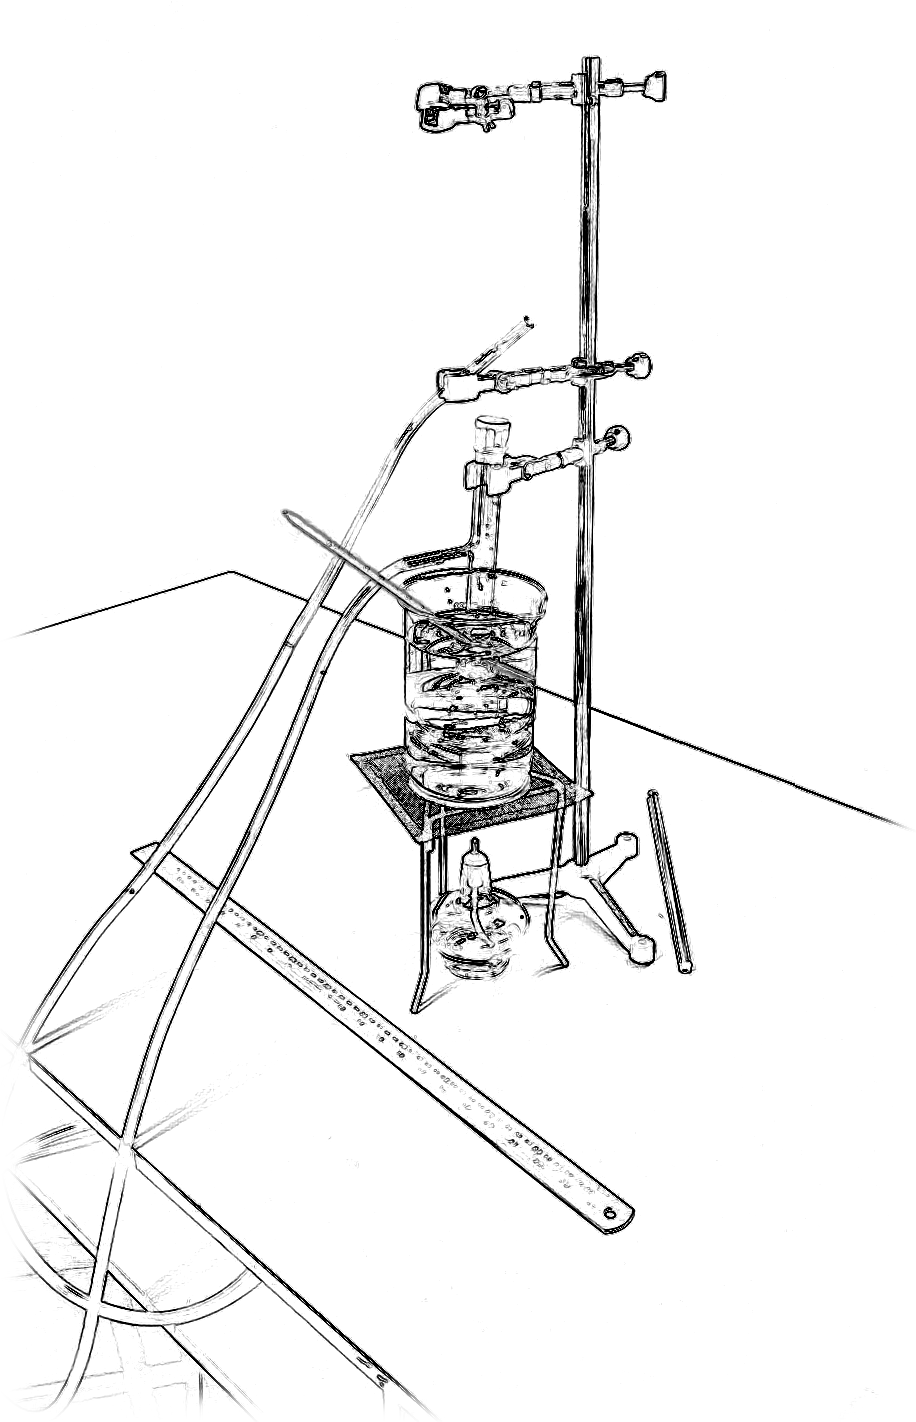
\includegraphics[width=0.7\textwidth]{Ilustrations/AparatoZeroAbs.png}
\caption{Aparato para a verificação do zero absoluto.}
\end{figure}
%%%%%%%%%%%%%%%%%%%%%%%%%%%%%%%%%%%%%%%%%%%%%%%%%%%%%%%%%%%%%%%%%%%%%%%%%%%%%%%
\section{Procedimento Experimental}
%%%%%%%%%%%%%%%%%%%%%%%%%%%%%%%%%%%%%%%%%%%%%%%%%%%%%%%%%%%%%%%%%%%%%%%%%%%%%%%

%%%%%%%%%%%%%%%%%%%%%%%%%%%%%%%%
\subsection{Montagem do aparato}
%%%%%%%%%%%%%%%%%%%%%%%%%%%%%%%%

\begin{enumerate}
\item Disponha a tela de amianto sobre o suporte e coloque o becker sobre ela;
\item Disponha o suporte vertical próximo ao becker. Afixe nele uma garra e a utilize para segurar o balão de destilação. A parte arredondada do balão deve ficar disposta dentro do becker, porém sem tocar o fundo;
\item Adicione água ao tubo de forma que ele fique sem bolhas e com água até aproximadamente \np[cm]{20} de cada extremidade;
\item Prenda o tubo ao suporte com o auxílio de garras de forma que uma das extremidades possa ser presa ao balão e que a outra fique à mesma altura que a primeira (a parte restante do tubo deve ficar abaixo da mesa, no chão);
\item Prenda uma das extremidades do tubo à saída lateral do balão de destilação;
\item Se o balão estiver com a extremidade superior aberta, feche-a com a rolha;
\item Adicione água ao becker até cobrir a parte arredondada do balão e parte do gargalo;
\end{enumerate}

%%%%%%%%%%%%%%%%%%%%%%%%%%%%%%%%%%%%%%%%%%%
\subsection{Coleta dos dados experimentais}
%%%%%%%%%%%%%%%%%%%%%%%%%%%%%%%%%%%%%%%%%%%

\begin{enumerate}
\item Verifique a pressão atmosférica $P_0$ e a anote na Tabela~\ref{Tab:Dados};
\item Verifique a temperatura da água com o termômetro e a anote na Tabela~\ref{Tab:Dados}.
\item Verifique a \emph{distância vertical}\footnote{Veja a Figura~\ref{Fig:FigEsquematicaTermGas}.} $h$ entre os topos das colunas d'água nas duas extremidades da mangueira (Veja a Figura~\ref{Fig:FigEsquematicaTermGas}) e a anote na Tabela~
\ref{Tab:Dados}.\footnote{Se a altura da coluna na extremidade do tubo ligada ao balão for maior que a da coluna na extremidade livre, o valor de $h$ deve ser marcado com um sinal negativo, pois a pressão no balão é menor que a atmosférica.}
\item Na extremidade do tubo ligada ao balão, marque com caneta a posição do topo da coluna d'água. Essa marca é importante pois ao tomarmos medidas da distância vertical $h$ precisamos garantir que o gás é mantido a volume constante.
\item Disponha a lamparina abaixo da tela de amianto e a acenda.
\item Agite a água constantemente com o bastão de vidro para que ela tenha uma temperatura homogênea; 
\item Assim que a temperatura aumentar \np[\tcdegree C]{2}, levante a extremidade livre do tubo de forma que o nível na extremidade ligada ao balão volte à posição original, marcada no passo anterior. Verifique o valor da temperatura\footnote{Meça a temperatura próximo da metade da parte arredondada do balão, visando evitar possíveis regiões de temperatura não uniforme (o ideal é apagar a lamparina e agitar a água por alguns segundos, anotando a temperatura atingida no equilíbrio térmico).} e a diferença vertical $h$ entre as colunas d'água e anote na Tabela~\ref{Tab:Dados}.
\item Aguarde até que a temperatura volte a subir \np[\tcdegree C]{2,0}, reajuste o nível da coluna d'água na extremidade do tubo ligada ao balão até que ele volte a coincidir com a marca inicial, e determine o novo valor de $h$. Anote os novos valores na Tabela~\ref{Tab:Dados}.
\item Repita o processo do item anterior de forma a obter o maior número de dados experimentais possível, ou completar a Tabela~\ref{Tab:Dados}.
\end{enumerate}

%%%%%%%%%%%%%%%%%%%%%%%%%%%%%%%%%%%%%%%%%%%%%%%%%%%%%%%%%%%%%%%%%%%%%%%%%%%%%%%
%%%%%%%%%%%%%%%%%%%%%%%%%%%%%%%%%%%%%%%%%%%%%%%%%%%%%%%%%%%%%%%%%%%%%%%%%%%%%%%
%%%%%%%%%%%%%%%%%%%%%%%%%%%%%%%%%%%%%%%%%%%%%%%%%%%%%%%%%%%%%%%%%%%%%%%%%%%%%%%
%%%%%%%%%%%%%%%%%%%%%%%%%%%%%%%%%%%%%%%%%%%%%%%%%%%%%%%%%%%%%%%%%%%%%%%%%%%%%%%
\cleardoublepage

\noindent{}{\huge\textit{Zero absoluto}}

\vspace{15mm}

\begin{fullwidth}
\noindent{}\makebox[0.6\linewidth]{Turma:\enspace\hrulefill}\makebox[0.4\textwidth]{  Data:\enspace\hrulefill}
\vspace{5mm}

\noindent{}\makebox[0.6\linewidth]{Aluno(a):\enspace\hrulefill}\makebox[0.4\textwidth]{  Matrícula:\enspace\hrulefill}

\noindent{}\makebox[0.6\linewidth]{Aluno(a):\enspace\hrulefill}\makebox[0.4\textwidth]{  Matrícula:\enspace\hrulefill}

\noindent{}\makebox[0.6\linewidth]{Aluno(a):\enspace\hrulefill}\makebox[0.4\textwidth]{  Matrícula:\enspace\hrulefill}

\noindent{}\makebox[0.6\linewidth]{Aluno(a):\enspace\hrulefill}\makebox[0.4\textwidth]{  Matrícula:\enspace\hrulefill}

\noindent{}\makebox[0.6\linewidth]{Aluno(a):\enspace\hrulefill}\makebox[0.4\textwidth]{  Matrícula:\enspace\hrulefill}
\end{fullwidth}

\vspace{5mm}

%%%%%%%%%%%%%%%%%%%%%%%%%%%%%%%%%%%%%%%%%%%%%%%%%%%%%%%%%%%%%%%%%%%%%%%%%%%%%%%
\section{Questionário}
%%%%%%%%%%%%%%%%%%%%%%%%%%%%%%%%%%%%%%%%%%%%%%%%%%%%%%%%%%%%%%%%%%%%%%%%%%%%%%%

\begin{question}[type={exam}]{1}
Apresente os resultados de maneira clara e organizada. Mostre os cálculos requisitados de maneira clara e sucinta, evidenciando o raciocínio desenvolvido.
\end{question}

\begin{question}[type={exam}]{1}
Liste os equipamentos utilizados. Para os instrumentos de medida, descreva o tipo do equipamento, sua resolução, e seu erro de escala.
\end{question}

\begin{question}[type={exam}]{1}
Preencha as tabelas com o número adequado de algarismos significativos, unidades, e erros de escala apropriados. 
\end{question}

\begin{question}[type={exam}]{1.5}
Elabore um gráfico de $P \times T$ para os dados da Tabela~\ref{Tab:Dados}.
\end{question}

\begin{question}[type={exam}]{1}
Calcule a reta que melhor representa os dados experimentais utilizando o método dos mínimos quadrados e a adicione ao gráfico.
\end{question}

\begin{question}[type={exam}]{1}
Utilizando as Equações~\ref{Eq:EqRazaoABZeroAbs1} e~\ref{Eq:EqRazaoABZeroAbs2} e os coeficientes para a regressão linear obtidos através do método de mínimos quadrados, calcule o valor de temperatura para o qual a pressão será zero. Verifique o erro percentual entre tal valor de temperatura e o valor de referência $T_0^{\textrm{ref}} = -\np[\tcdegree C]{273,15}$ através da expressão
\begin{equation}
	E_{\%} = \left|\frac{x-x_{\textrm{ref}}}{x_{\textrm{ref}}}\right| \times 100.
\end{equation}
\end{question}

\begin{question}[type={exam}]{2}
Calcule os erros associados aos coeficientes $A$ e $B$ da regressão linear e ---~a partir dos coeficientes, dos erros a eles associados, e das Equações~\ref{Eq:EqRazaoABZeroAbs1} e~\ref{Eq:EqRazaoABZeroAbs2}~---  calcule o erro associado a $T_C^0$.
\end{question}

\begin{question}[type={exam}]{1.5}
Considerando os objetivos do experimento, listados na Seção~\ref{Sec:ObjetivosZeroAbsoluto}, e os resultados obtidos nas questões anteriores, discuta quais objetivos foram atingidos com sucesso, justificando suas conclusões. Se algum objetivo não foi atingido, discuta quais são os possíveis motivos do fracasso e que providências podem ser tomadas para que eles sejam alcançados.
\end{question}

%%%%%%%%%%%%%%%%%%%%%%%%%%%%%%%%%%%%%%%%%%%%%%%%%%%%%%%%%%%%%%%%%%%%%%%%%%%%%%%
\section{Tabelas}
%%%%%%%%%%%%%%%%%%%%%%%%%%%%%%%%%%%%%%%%%%%%%%%%%%%%%%%%%%%%%%%%%%%%%%%%%%%%%%%

\begin{table*}[!htb]
\caption{Dados para a altura da coluna de água em função da temperatura.}
\label{Tab:Dados}
	\begin{center}
		\begin{tabular}{cp{45mm}p{45mm}p{45mm}c}
		\toprule
		&\multicolumn{2}{l}{\textbf{Constantes}}\\
		\cmidrule{2-3}
		& \cellcolor[gray]{0.89} $P_0$ &\cellcolor[gray]{0.92} \\
		& \cellcolor[gray]{0.95} $\rho$ & \cellcolor[gray]{0.97}\\
		\cmidrule{2-3}
		\\
		&\multicolumn{2}{l}{\textbf{Dados para a altura da coluna}} \\
		\cmidrule{2-4}
		& $T$ & $h$ & $P$ & \\
		\cmidrule{2-4}
		& \cellcolor[gray]{0.89} & \cellcolor[gray]{0.92} & \cellcolor[gray]{0.89} \\
		& \cellcolor[gray]{0.95} & \cellcolor[gray]{0.97} & \cellcolor[gray]{0.95} \\
		& \cellcolor[gray]{0.89} & \cellcolor[gray]{0.92} & \cellcolor[gray]{0.89} \\
		& \cellcolor[gray]{0.95} & \cellcolor[gray]{0.97} & \cellcolor[gray]{0.95} \\
		& \cellcolor[gray]{0.89} & \cellcolor[gray]{0.92} & \cellcolor[gray]{0.89} \\
		& \cellcolor[gray]{0.95} & \cellcolor[gray]{0.97} & \cellcolor[gray]{0.95} \\
		& \cellcolor[gray]{0.89} & \cellcolor[gray]{0.92} & \cellcolor[gray]{0.89} \\
		& \cellcolor[gray]{0.95} & \cellcolor[gray]{0.97} & \cellcolor[gray]{0.95} \\
		& \cellcolor[gray]{0.89} & \cellcolor[gray]{0.92} & \cellcolor[gray]{0.89} \\
		& \cellcolor[gray]{0.95} & \cellcolor[gray]{0.97} & \cellcolor[gray]{0.95} \\
		\cmidrule{2-4}
		\bottomrule
		\end{tabular}
	\end{center}
\end{table*}



\printbibliography
\cleardoublepage
\thispagestyle{empty}
\begin{figure*}
\centering
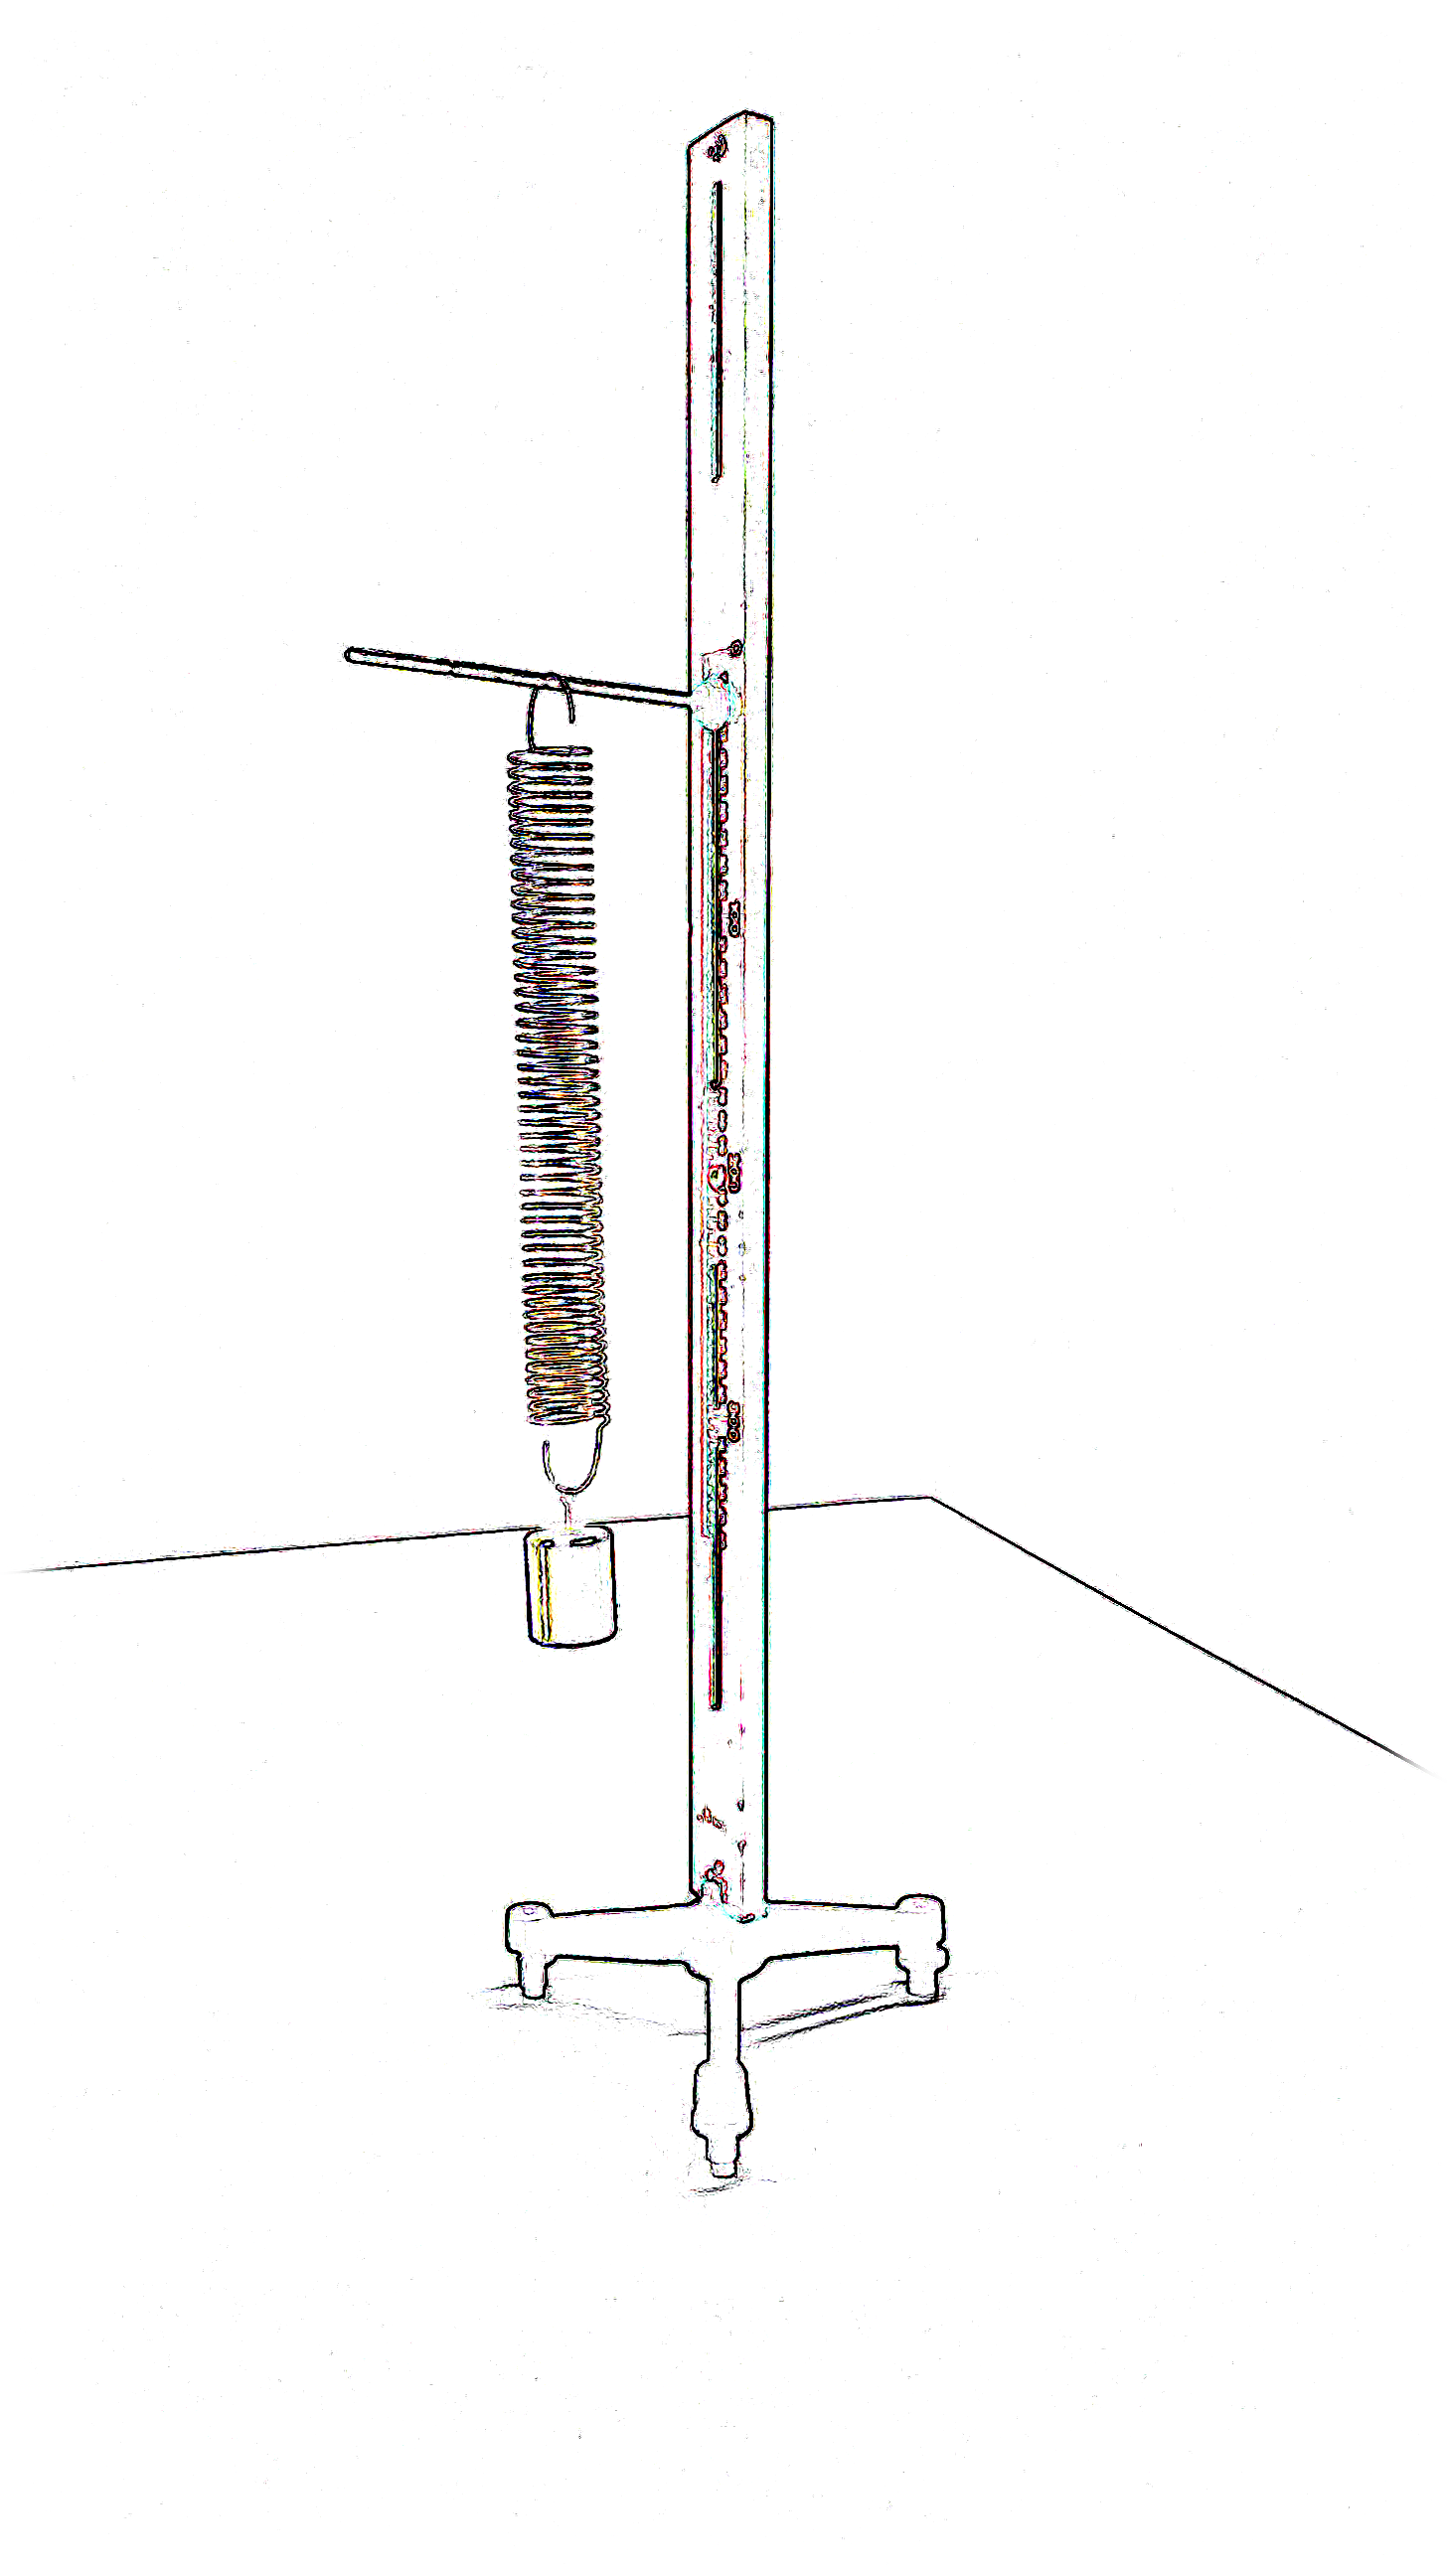
\includegraphics[width = 0.5\linewidth]{Ilustrations/Massa-Mola.png}
\end{figure*}
\vfill
\begin{fullwidth}
\begin{center}\sc
Elaborado usando \LaTeX \\
documentclass: tufte-book \\
imagens tratadas usando Gimp \\
Figuras elaboradas usando tikz
\end{center}
\end{fullwidth}
\end{document}
